% Options for packages loaded elsewhere
\PassOptionsToPackage{unicode}{hyperref}
\PassOptionsToPackage{hyphens}{url}
%
\documentclass[
  10pt,
]{book}
\usepackage{amsmath,amssymb}
\usepackage{iftex}
\ifPDFTeX
  \usepackage[T1]{fontenc}
  \usepackage[utf8]{inputenc}
  \usepackage{textcomp} % provide euro and other symbols
\else % if luatex or xetex
  \usepackage{unicode-math} % this also loads fontspec
  \defaultfontfeatures{Scale=MatchLowercase}
  \defaultfontfeatures[\rmfamily]{Ligatures=TeX,Scale=1}
\fi
\usepackage{lmodern}
\ifPDFTeX\else
  % xetex/luatex font selection
    \setmainfont[Numbers=OldStyle]{Charis SIL}
  \newfontfamily{\arabicfont}[Script=Arabic,Scale=1.0]{Vazirmatn-Light}
  \newfontfamily{\tradarab}[Script=Arabic,Scale=1.0]{Amiri}
  \newfontfamily{\tradarabsmall}[Script=Arabic,Scale=0.75]{Amiri}
\fi
% Use upquote if available, for straight quotes in verbatim environments
\IfFileExists{upquote.sty}{\usepackage{upquote}}{}
\IfFileExists{microtype.sty}{% use microtype if available
  \usepackage[]{microtype}
  \UseMicrotypeSet[protrusion]{basicmath} % disable protrusion for tt fonts
}{}
\makeatletter
\@ifundefined{KOMAClassName}{% if non-KOMA class
  \IfFileExists{parskip.sty}{%
    \usepackage{parskip}
  }{% else
    \setlength{\parindent}{0pt}
    \setlength{\parskip}{6pt plus 2pt minus 1pt}}
}{% if KOMA class
  \KOMAoptions{parskip=half}}
\makeatother
\usepackage{xcolor}
\usepackage[paperwidth=156mm,paperheight=234mm,bindingoffset=16mm,textwidth=114.8mm,textheight=170.8mm,twoside]{geometry}
\usepackage{longtable,booktabs,array}
\usepackage{calc} % for calculating minipage widths
% Correct order of tables after \paragraph or \subparagraph
\usepackage{etoolbox}
\makeatletter
\patchcmd\longtable{\par}{\if@noskipsec\mbox{}\fi\par}{}{}
\makeatother
% Allow footnotes in longtable head/foot
\IfFileExists{footnotehyper.sty}{\usepackage{footnotehyper}}{\usepackage{footnote}}
\makesavenoteenv{longtable}
\usepackage{graphicx}
\makeatletter
\def\maxwidth{\ifdim\Gin@nat@width>\linewidth\linewidth\else\Gin@nat@width\fi}
\def\maxheight{\ifdim\Gin@nat@height>\textheight\textheight\else\Gin@nat@height\fi}
\makeatother
% Scale images if necessary, so that they will not overflow the page
% margins by default, and it is still possible to overwrite the defaults
% using explicit options in \includegraphics[width, height, ...]{}
\setkeys{Gin}{width=\maxwidth,height=\maxheight,keepaspectratio}
% Set default figure placement to htbp
\makeatletter
\def\fps@figure{htbp}
\makeatother
\setlength{\emergencystretch}{3em} % prevent overfull lines
\providecommand{\tightlist}{%
  \setlength{\itemsep}{0pt}\setlength{\parskip}{0pt}}
\setcounter{secnumdepth}{5}
\ifLuaTeX
\usepackage[bidi=basic]{babel}
\else
\usepackage[bidi=default]{babel}
\fi
\babelprovide[main,import]{english}
\ifPDFTeX
\else
\babelfont{rm}[Numbers=OldStyle]{Charis SIL}
\fi
\babelprovide[import]{arabic}
% get rid of language-specific shorthands (see #6817):
\let\LanguageShortHands\languageshorthands
\def\languageshorthands#1{}
\newcommand{\gitTag}{\input|"git describe"}
\usepackage{lipsum}
\usepackage{metalogo}
\usepackage{xcolor}
\usepackage{url}
\usepackage{fancyhdr}

% To use New Computer Modern font, uncomment following two lines only
%\defaultfontfeatures{Numbers=OldStyle} % have to load this first, before loading fontsetup
%\usepackage[default]{fontsetup} % "default" option loads book weight.
%\addfontfeature{Numbers=Lowercase} % don't need this

% section style, all section headings normal size
\usepackage{sectsty}
\allsectionsfont{\normalsize}


% section style, all section headings normal size bold, except chapter headings
\usepackage[bf,tiny]{titlesec}
%\definecolor{gray75}{gray}{0.5}
%\titleformat*{\chapter}      {\normalfont\normalsize\color{gray75}}
%\titleformat*{\section}      {\normalfont\normalsize\color{gray75}}
%\titleformat*{\subsection}   {\normalfont\normalsize\color{gray75}}
%\titleformat*{\subsubsection}{\normalfont\normalsize\color{gray75}}

% Arabic font's ascenders, descenders, and diacritics increase Latex's line
% spacing irregularly for some lines more than others to result in a visually
% unappealing output.
%
% I tried setting \lineskiplimit=-\maxdimen as some had suggested this but it
% completely destroys linespacing in tables and around tikzpictures.
%
% Then I found that \smash forces a 0 depth and 0 height for it's argument. So
% the Arabic text is ignored by Latex for line spacing purposes. Call \smash on
% the Arabic text input to babel's \foreignlanguage as below.
%
% I also tried calling smash on the output of \foreignlanguage but that seemed
% to cause problems on chapter headings.
%
% However, with this solution, some itemized lists have Arabic text directly on
% top of each other and the diacritics collide. For these lists insert a
% \vphantom{\huge J} for each item to locally increase line spacing. See
% examples in script.Rmd and inna_and_its_sisters.Rmd.
%
% The other unsolved issue with the solution is that it messes up the bidi dir
% in the sidebar contents in my PDF reader
\AddBabelHook[arabic]{smash}{foreign}{\def\BabelText##1{\smash{##1}}}

% Add section symbol § to every (sub)section heading and reference
%\NewCommandCopy{\oldthesection}{\thesection}
%\renewcommand{\thesection}{\S\oldthesection}

% Fancy header

% use this command from preface
%\newcommand{\forcefancyhdr}[1]{\markboth {\textsc{\MakeLowercase{#1}}}{\textsc{\MakeLowercase{#1}}}}

\renewcommand{\chaptermark}[1]{\markboth {\textsc{\MakeLowercase{\scalebox{1}[0.81]{\thechapter}\quad #1}}}{}}
\renewcommand{\sectionmark}[1]{\markright{\textsc{\MakeLowercase{\scalebox{1}[0.81]{\S\thesection}\ }}}}

% Start fancy header style beginning here, override with thispagestyle{empty} for copyright page
\pagestyle{fancy}

\fancypagestyle{mymainstyle}{%
\fancyhf{}
%\fancyhead[LE]{\thepage\phantom{xxx}\itshape\nouppercase{Fundamentals of Standard Arabic}}
%\fancyhead[RO]{\itshape\nouppercase{\leftmark}\phantom{xxx}\thepage}
%\fancyhead[LE]{\thepage \ {\vrule height 13pt width 1pt} \itshape\nouppercase{Fundamentals of Standard Arabic}}
%\fancyhead[RO]{\itshape\nouppercase{\leftmark} \ {\vrule height 13pt width 1pt} \thepage}

%\fancyhead[LE]{\leavevmode\smash{\llap{\thepage\ \rule[-0.5em]{1pt}{1.5em}}}\phantom{x}\itshape\nouppercase{Fundamentals of Standard Arabic}}
%\fancyhead[RO]{\textsl{\nouppercase{\leftmark}}\phantom{x}\leavevmode\smash{\rlap{\rule[-0.5em]{1pt}{1.5em}\ \thepage}}}
%\fancyhead[LO]{\itshape\nouppercase{\rightmark}}
%\fancyhead[LO,RE]{\textsl{\nouppercase{https://adamiturabi.github.io/arabic-tutorial-book/}}}

% Put page numbers outside text block in top margin
%\fancyhead[LE]{\hspace*{-1cm}\thepage}
%\fancyhead[RO]{\thepage\hspace*{-1cm}}

% Put page numbers inside text block in top margin
\fancyhead[LE,RO]{\scalebox{1}[0.81]{\thepage}}

\fancyhead[CO]{\nouppercase{\rightmark}}
\fancyhead[CE]{\nouppercase{\leftmark}}
\renewcommand{\headrulewidth}{0pt}

\fancyfoot[RE, RO]{\phantom{xxx}\\\phantom{xxx}\\\phantom{xxx}\\\phantom{xxx}\\\textcolor{gray}{\tiny{Author Names, \textit{A Learner's Grammar of Classical Standard Arabic}, \texttt{\gitTag}\\\url{https://adamiturabi.github.io/arabic-tutorial-book/}}}}

}% definition of mymainstyle

% Footer for chapter start pages:
\fancypagestyle{plain}{%
\fancyhf{}
\fancyfoot[RE, RO]{\phantom{xxx}\\\phantom{xxx}\\\phantom{xxx}\\\phantom{xxx}\\\textcolor{gray}{\tiny{Author Names, \textit{A Learner's Grammar of Classical Standard Arabic}, \texttt{\gitTag}\\\url{https://adamiturabi.github.io/arabic-tutorial-book/}}}}
\fancyfoot[CO]{\scalebox{1}[0.81]{\thepage}}
}

% Blank pages (e.g., left hand pages between chapters should be completely blank. no headers even
\makeatletter
\def\cleardoublepage{\clearpage\if@twoside \ifodd\c@page\else
  \begingroup
    \mbox{}
    \vspace*{\fill}
    \begin{center}
      %This page intentionally contains only this sentence.
    \end{center}
    \vspace{\fill}
    \thispagestyle{empty}
    \newpage
    \if@twocolumn\mbox{}\newpage\fi
  \endgroup\fi\fi}
\makeatother

\usepackage[color={[gray]{0.85}}, fontsize=32pt, text={Work in progress. Not ready for study.}]{draftwatermark}

\widowpenalty10000
%\clubpenalty10000

\babelfont[arabic]{rm}
          [Language=Default]{Vazirmatn-Light}
\babelfont[arabic]{sf}
          [Language=Default]{Vazirmatn-Light}

% Customize ToC table of contents
\usepackage[titles]{tocloft}

% Reserve horizontal spacing for chapter and section numbers
\setlength{\cftchapnumwidth}{3em}
\setlength{\cftsecnumwidth}{3em}

% No dots between chapter/section name and page number
\renewcommand{\cftchapdotsep}{\cftnodots}
\renewcommand{\cftsecdotsep}{\cftnodots}

% Some horizontal space between chapter/section name and page number
\renewcommand{\cftchapleader}{\quad}
\renewcommand{\cftsecleader} {\quad}
\renewcommand{\cftchapafterpnum}{\cftparfillskip}
\renewcommand{\cftsecafterpnum}{\cftparfillskip}
% Page number aligned left instead of right
\renewcommand{\cftpnumalign}{l}

% Chapter and section name font sizes
\renewcommand\cftchapfont{\normalfont}
\renewcommand\cftsecfont{\footnotesize}

% Chapter and section page number font sizes
\renewcommand\cftchappagefont{\normalfont}
\renewcommand\cftsecpagefont{\footnotesize}

% Short/brief table of contents before detailed one
% See frontpage.tex for additional customization there
\usepackage[tight]{shorttoc}

% Change title of original ToC to contrast with shorttoc title
\addto\captionsenglish{% Replace "english" with the language you use
  \renewcommand{\contentsname}%
    {Detailed Contents}%
}
\ifLuaTeX
  \usepackage{selnolig}  % disable illegal ligatures
\fi
\usepackage{csquotes}
\usepackage{bookmark}
\IfFileExists{xurl.sty}{\usepackage{xurl}}{} % add URL line breaks if available
\urlstyle{same}
\hypersetup{
  pdfauthor={Author Names},
  pdflang={en},
  hidelinks,
  pdfcreator={LaTeX via pandoc}}

\title{A Learner's Grammar of\\
Classical Standard Arabic}
\author{Author Names}
\date{v0.1.0-879-gd5f7913}

\begin{document}
\maketitle

\thispagestyle{empty}
%% copyrightpage
\begingroup
\footnotesize
\parindent 0pt
\parskip \baselineskip
\textcopyright{} 2023 Author Names \\
All rights reserved.

    This work may not be distributed or modified, without written permission from the copyright holder.

%\begin{center}
%\begin{tabular}{ll}
\texttt{\gitTag}
%\end{tabular}
%\end{center}

This book is typeset with \XeLaTeX\ (via the R bookdown package and the pandoc document converter)
in the Charis, Vazirmatn, and Amiri typefaces.


\vfill


%%%%{\LARGE\plogo}
%\vspace*{2\baselineskip}


\endgroup
\clearpage

\newpage
% Force Latex to begin Main matter headers and pagination from the very beginning
%\mainmatter
\pagestyle{mymainstyle}
\begingroup
% For short ToC remove vertical spacing between lines for more condensed look
%\setlength{\cftparskip}{-2pt}
\setlength{\cftbeforechapskip}{-3pt}
\shorttableofcontents{Brief Contents}{0}
\endgroup


{
\setcounter{tocdepth}{1}
\tableofcontents
}
\chapter*{Preface}\label{preface}
\addcontentsline{toc}{chapter}{Preface}

\markboth {\textsc{\MakeLowercase{Preface}}}{\textsc{\MakeLowercase{Preface}}}

\begin{center}
\tradarab{
الرحيم
الرحمن
الله
بسم
}
\end{center}

The primary texts of Islām (the Qurʾān and the Ḥadīt͡h) are in Arabic. So too is much of its scholarly literature. However, there is a multitude of Muslims for whom Arabic is not a native language, yet who are familiar enough with English to study textbooks written in this language. The goal of this book is to help them learn Arabic at a beginner's level so that, together with a study of the appropriate expositional texts, they are one step closer to understanding the primary texts in their original language. We hope that this will, if Allāh wills, make them feel more connected to the primary texts and their teachings. Furthermore, they can be empowered to study the vast body of Arabic Islāmic literature.

This book is a learning grammar and not a reference grammar.
So, in the initial chapters, topics are introduced at only a basic level, without treating them exhaustively, before moving on to the next topic.
That notwithstanding, past the first few chapters, we have generally tried to group content meaningfully for convenient reference during learning.
In addition, since this is a beginner's textbook, only the more common usages are explained.

We have also aimed to make this a self-instruction textbook so that a diligent student should, if Allāh wills, be able to study it without an instructor. The target learner is someone who has not been exposed to grammatical terminology like \emph{inflection}, \emph{case}, \emph{mood}, etc. While terminology is necessary for a rigorous non-immersive learning of language, we have tried to steer away from Latin-based terms like \emph{accusative} and \emph{jussive}. Such terms, when first encountered by an uninitiated learner, may deter from proceeding further. (Learning a language can be hard enough without getting the feeling that your grammar book is accusing you of something!) So we have in some places translated the meaning of Arabic grammar terms to English. In other places, we have used established English grammar terms where the terms are basic enough. We have even, in places, invented terms where we deemed appropriate. The drawback to this non-standard approach, however, is that the student may not be able to immediately relate the terminology he has learned in this book to established terminology in other grammar textbooks. To remedy this to some extent, we provide a glossary in the appendix which maps the grammatical terminology used in this book to other, established, Latin-based and Arabic-based counterparts.

It may also be appropriate to inform the reader that we chose to present a simplified version of Arabic grammar. As such, the grammar presented here may not be entirely consistent with the comprehensive and harmonious framework developed by the Arab grammarians. We chose this approach because we felt that exposing the beginner to complex grammatical details at this stage would be more of a hindrance than a help in learning the language.

This book is a currently work in progress and is produced with the R bookdown package. The code and text for volume~1 are open-sourced and developed at
\href{https://github.com/adamiturabi/arabic-tutorial-book}{github.com/adamiturabi/arabic-tutorial-book}.
The typeset output of volume~1 is published at
\href{https://adamiturabi.github.io/arabic-tutorial-book/}{adamiturabi.github.io/arabic-tutorial-book/}.

\textsc{the authors}

\chapter*{Romanization scheme}\label{romanization-scheme}
\addcontentsline{toc}{chapter}{Romanization scheme}

\markboth {\textsc{\MakeLowercase{Romanization scheme}}}{\textsc{\MakeLowercase{Romanization scheme}}}

The following romanization scheme is used in this book for the transcription and transliteration of Arabic sounds and letters into the Latin script.

\textsc{consonants}

\begin{longtable}[]{@{}
  >{\centering\arraybackslash}p{(\columnwidth - 26\tabcolsep) * \real{0.0714}}
  >{\centering\arraybackslash}p{(\columnwidth - 26\tabcolsep) * \real{0.0714}}
  >{\centering\arraybackslash}p{(\columnwidth - 26\tabcolsep) * \real{0.0714}}
  >{\centering\arraybackslash}p{(\columnwidth - 26\tabcolsep) * \real{0.0714}}
  >{\centering\arraybackslash}p{(\columnwidth - 26\tabcolsep) * \real{0.0714}}
  >{\centering\arraybackslash}p{(\columnwidth - 26\tabcolsep) * \real{0.0714}}
  >{\centering\arraybackslash}p{(\columnwidth - 26\tabcolsep) * \real{0.0714}}
  >{\centering\arraybackslash}p{(\columnwidth - 26\tabcolsep) * \real{0.0714}}
  >{\centering\arraybackslash}p{(\columnwidth - 26\tabcolsep) * \real{0.0714}}
  >{\centering\arraybackslash}p{(\columnwidth - 26\tabcolsep) * \real{0.0714}}
  >{\centering\arraybackslash}p{(\columnwidth - 26\tabcolsep) * \real{0.0714}}
  >{\centering\arraybackslash}p{(\columnwidth - 26\tabcolsep) * \real{0.0714}}
  >{\centering\arraybackslash}p{(\columnwidth - 26\tabcolsep) * \real{0.0714}}
  >{\centering\arraybackslash}p{(\columnwidth - 26\tabcolsep) * \real{0.0714}}@{}}
\toprule\noalign{}
\endhead
\bottomrule\noalign{}
\endlastfoot
\foreignlanguage{arabic}{ص} & \foreignlanguage{arabic}{ش} & \foreignlanguage{arabic}{س} & \foreignlanguage{arabic}{ز} & \foreignlanguage{arabic}{ر} & \foreignlanguage{arabic}{ذ} & \foreignlanguage{arabic}{د} & \foreignlanguage{arabic}{خ} & \foreignlanguage{arabic}{ح} & \foreignlanguage{arabic}{ج} & \foreignlanguage{arabic}{ث} & \foreignlanguage{arabic}{ت} & \foreignlanguage{arabic}{ب} & \foreignlanguage{arabic}{ء} \\
ṣ & s͡h & s & z & r & d͡h & d & k͡h & ḥ & j & t͡h & t & b & ʾ \\
\end{longtable}

\begin{longtable}[]{@{}
  >{\centering\arraybackslash}p{(\columnwidth - 26\tabcolsep) * \real{0.0714}}
  >{\centering\arraybackslash}p{(\columnwidth - 26\tabcolsep) * \real{0.0714}}
  >{\centering\arraybackslash}p{(\columnwidth - 26\tabcolsep) * \real{0.0714}}
  >{\centering\arraybackslash}p{(\columnwidth - 26\tabcolsep) * \real{0.0714}}
  >{\centering\arraybackslash}p{(\columnwidth - 26\tabcolsep) * \real{0.0714}}
  >{\centering\arraybackslash}p{(\columnwidth - 26\tabcolsep) * \real{0.0714}}
  >{\centering\arraybackslash}p{(\columnwidth - 26\tabcolsep) * \real{0.0714}}
  >{\centering\arraybackslash}p{(\columnwidth - 26\tabcolsep) * \real{0.0714}}
  >{\centering\arraybackslash}p{(\columnwidth - 26\tabcolsep) * \real{0.0714}}
  >{\centering\arraybackslash}p{(\columnwidth - 26\tabcolsep) * \real{0.0714}}
  >{\centering\arraybackslash}p{(\columnwidth - 26\tabcolsep) * \real{0.0714}}
  >{\centering\arraybackslash}p{(\columnwidth - 26\tabcolsep) * \real{0.0714}}
  >{\centering\arraybackslash}p{(\columnwidth - 26\tabcolsep) * \real{0.0714}}
  >{\centering\arraybackslash}p{(\columnwidth - 26\tabcolsep) * \real{0.0714}}@{}}
\toprule\noalign{}
\endhead
\bottomrule\noalign{}
\endlastfoot
\foreignlanguage{arabic}{ى} & \foreignlanguage{arabic}{و} & \foreignlanguage{arabic}{ه} & \foreignlanguage{arabic}{ن} & \foreignlanguage{arabic}{م} & \foreignlanguage{arabic}{ل} & \foreignlanguage{arabic}{ک} & \foreignlanguage{arabic}{ق} & \foreignlanguage{arabic}{ف} & \foreignlanguage{arabic}{غ} & \foreignlanguage{arabic}{ع} & \foreignlanguage{arabic}{ظ} & \foreignlanguage{arabic}{ط} & \foreignlanguage{arabic}{ض} \\
y & w & h & n & m & l & k & q & f & g͡h & ɛ & ḍ͡h & ṭ & ḍ \\
\end{longtable}

\textsc{vowels}

\begin{longtable}[]{@{}
  >{\centering\arraybackslash}p{(\columnwidth - 14\tabcolsep) * \real{0.1250}}
  >{\centering\arraybackslash}p{(\columnwidth - 14\tabcolsep) * \real{0.1250}}
  >{\centering\arraybackslash}p{(\columnwidth - 14\tabcolsep) * \real{0.1250}}
  >{\centering\arraybackslash}p{(\columnwidth - 14\tabcolsep) * \real{0.1250}}
  >{\centering\arraybackslash}p{(\columnwidth - 14\tabcolsep) * \real{0.1250}}
  >{\centering\arraybackslash}p{(\columnwidth - 14\tabcolsep) * \real{0.1250}}
  >{\centering\arraybackslash}p{(\columnwidth - 14\tabcolsep) * \real{0.1250}}
  >{\centering\arraybackslash}p{(\columnwidth - 14\tabcolsep) * \real{0.1250}}@{}}
\toprule\noalign{}
\endhead
\bottomrule\noalign{}
\endlastfoot
\foreignlanguage{arabic}{◌َ} & \foreignlanguage{arabic}{◌ُ} & \foreignlanguage{arabic}{◌ِ} & \foreignlanguage{arabic}{◌َا} & \foreignlanguage{arabic}{◌ُو} & \foreignlanguage{arabic}{◌ِي} & \foreignlanguage{arabic}{◌َوْ} & \foreignlanguage{arabic}{◌َيْ} \\
a & u & i & ā & ū & ī & aw & ay \\
\end{longtable}

When transcribing example text,
the \emph{italic} Latin script is used,
no letters are capitalized,
a non-sentence-initial connecting hamzah is transliterated with a hyphen (-),
and the lām of the definite article is not transliterated for sun letters.
\foreignlanguage{arabic}{ة} is transcribed as \emph{h} at the end of an utterance, and as \emph{t} otherwise.
For example:

\foreignlanguage{arabic}{ٱِلْتَقَطَتْ أُمُّ طَلْحَةَ وَٱلْحَسَنِ وَرَقَةَ ٱلشَّجَرَةِ.}\\
\emph{ʾiltaqaṭat ʾummu ṭalḥata wa-lḥasani waraqata -s͡hs͡hajarah.}

When using Arabic words in the English text,
the regular (non-italic) Latin script is used,
words are transcribed in pausal pronunciation,
word-final \foreignlanguage{arabic}{◌ِيّ} \emph{-iyy} is transcribed as \enquote{ī},
the first letter of a proper noun is capitalized,
word-initial hamzah is not transliterated,
the definite article is always transliterated as \enquote{al-} with a hyphen following it,
as shown.
\foreignlanguage{arabic}{ة} is transcribed as \enquote{t} in the middle of an annexation, and as \enquote{h} otherwise.
Accurate romanizations are preferred unless an established and distinctly separate usage is current in English.
Examples:

\enquote{Ɛalī and Usāmah revised Sūrat al-Ɛankabūt from the Qurʾān in the mosque in the month of Rabīɛ al-T͡hānī.}

\enquote{The caliphate moved from al-Madīnah to Damascus.}

\chapter{Introduction}\label{introduction}

All praises are due to Allāh. We praise Him, seek His help, and ask for His forgiveness. We seek refuge in Allāh from the evil in our souls and from our sinful deeds. Whomever Allāh guides, no one can mislead. Whomever Allāh leads astray, no one can guide. I bear witness that there is no one worthy of worship except Allāh. I also bear witness that Muḥammad is His servant and messenger.

May the peace and blessings of Allāh be upon the Prophet Muḥammad, his family, his companions, and those who followed them with good conduct.

\section{History of Arabic}\label{history-of-arabic}

Allāh, may He be glorified and exalted, revealed the Qurʾān 1400 years ago to the Prophet Muḥammad, may Allāh grant peace and confer blessing upon him. The language of the Qurʾān is the Arabic language, as it was understood by the Arabs at that time.
The sayings and actions of the Prophet, may Allāh grant peace and confer blessing upon him, were recorded by his companions also in this Arabic language.
We will call the Arabic of this pre-Islāmic and early Islāmic era as Classical Arabic.
The Classical Arabic language consisted of multiple dialects that were spoken by the different tribes and in the different regions of the Arabian peninsula.

All languages change naturally over time. For example, English has changed to such a degree that the Old English language spoken 1400 years ago would be unintelligible to us today. So too did the Classical Arabic dialects begin to change. But as part of preserving His religion, Allāh preserved the Arabic language as well. This was by means of the efforts of scholars who recorded the Classical Arabic language of the time of the revelation.

In the process of preserving Arabic, one particular variety became standardized and gained prevalence as a literary language over the other dialects of the Arabic of the early-Islāmic period. This \emph{Standard Arabic}, in its early period after standardization, is called Classical Standard Arabic.
The pre-Islāmic and early Islāmic Arabic dialects (of which Classical Standard Arabic is but a standardized variety) are then referred to, collectively, as pre-standard Classical Arabic. Classical Standard Arabic was used as the language of religious scholarship, science, and literature in the Islāmic world. As scholars developed new branches of religious and secular sciences, new terms and meanings were added to it that are termed post-classical. A few words were also borrowed from foreign languages and Arabicized, as needed by the different scientific disciplines. (Pre-Standard Classical Arabic itself had a few Arabicized foreign borrowings from neighboring languages.) These additions were, by and large, deliberate, done by scholars who were experts in their fields and also well versed in Classical Standard Arabic, and validated by subsequent generations of scholarly discourse. Besides these needed additions, the grammar and core language remained remarkably unchanged.

While Standard Arabic was thus preserved from major change and was used for literary purposes, the language that was spoken by Arabs in their day-to-day lives continued to change over time from the pre-standard Classical Arabic dialects into the modern colloquial dialects. And so today, there exist two very distinct types of Arabic: the preserved Standard Arabic which is taught at schools and is primarily a written language, and the modern colloquial Arabic dialects which Arabs learn as their mother tongue and which are primarily only spoken and not written.

\begin{figure}
\centering
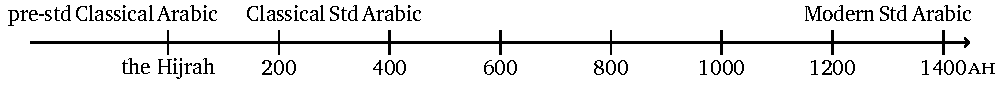
\includegraphics{A-Learners-Grammar-of-Classical-Standard-Arabic_files/figure-latex/unnamed-chunk-3-1.pdf}
\caption{\label{fig:unnamed-chunk-3}Timeline of the development of Standard Arabic.}
\end{figure}

In modern times, many new words and meanings have been added to Standard Arabic, often via translation from Western languages, to keep up with technological advancements and modern media.
This modern development of Standard Arabic is called Modern Standard Arabic.
There are also a small amount of words, meanings, and grammatical usages, which existed in Classical Arabic, but which are deemed archaic, and are therefore largely unused, in Modern Standard Arabic.

Figure~1.1 (above) depicts this historical development of Standard Arabic.

\section{\texorpdfstring{About this book }{About this book }}\label{about-this-book}

\subsection{Scope}\label{scope}

In this book, we will study Standard Arabic. We will focus on the pre-modern language. If Allāh wills, this will help you to begin to understand the language of the Qurʾān, the Ḥadīt͡h, and Islāmic literature.

If your goal is to learn Modern Standard Arabic, then this book may still be of help because the core language and the grammar are essentially the same. However, you may prefer to study from a resource that focuses on the modern language.

This book does not touch at all upon the modern colloquial dialects that are spoken in the Arab world today.

\subsection{Current status}\label{current-status}

This book is currently a work in progress, and not yet ready for study.
There is a watermark on all online published pages indicating this status.
The preface and this introduction have been written prematurely as a reference for guiding principles that we can refer to during the write process.
We publish updates online while the book is still a work in progress in the hope that it will help in correcting errors.

\subsection{Methodology}\label{methodology}

We will start, if Allāh wills, with the Arabic script and present, in each chapter, a new concept of Arabic grammar, together with examples.
We will also give vocabulary for you to memorize and have chapter exercises.

Many times we introduce a topic early on because a later topic is dependent on it.
And in order to organize content in a manageable and referrable way, we will give a full treatment of the first topic.
But in actuality, an exhaustive understanding of the first topic is not that very essential to the core understanding of grammar that a learner needs at that stage.
An example of such a topic is proper nouns which are, what we have termed, \emph{semi-flexible} (\emph{diptotes} in Western grammars), and indeed semi-flexible nouns in general.

In the chapter introductions, we will list any such topics contained in the chapter.
When encountering such topics for the first time, we recommend that you skim through them to get a basic understanding and move on to more essential concepts.
You may refer back to the topic when needed.

Some of the sentences we present, both as examples and as chapter exercises, because of their contrived nature, may seem of dubious usefulness to a learner wanting to learn practical usage.
Also, when translating examples, we usually steer toward a literal, word-for-word, translation rather than an idiomatic one.
The resulting English will then often sound awkward, and even sometimes ungrammatical.
This is to show a correspondence between the words in the Arabic sentence and the English translation.
We ask that you overlook these shortcomings.

\subsection{How to study}\label{how-to-study}

\subsubsection{Exercises}\label{exercises}

In answering the exercises, we strongly recommend that you memorize the vocabulary in full and write down the answers with pen and paper.
We strongly recommend that you
resist the tendency to
answer the exercises only orally or mentally without writing them down,
or look up the answers from the answer key before attempting to write the answer yourself,
or look up words in the vocabulary list without memorizing them,
or proceed to the next chapter before memorizing the vocabulary and going through the exercises.
You may also find yourself having to go back a few chapters every once in a while and revising the concepts therein.
This is very normal and not a cause for any concern. It may also prove beneficial to re-do the exercises of that chapter when doing so.

\subsubsection{Vocabulary}\label{vocabulary}

Know that while Arabic grammar requires effort to master to a proficient degree, the real barrier to reading and understanding Arabic texts by oneself is vocabulary.
Arabic is a very rich language and knowledge of a few thousand words is needed before the student can begin to read texts independently.
In fact, we would not be too far off to say that grammar, at this stage, is only a tool to help you make sense of the vocabulary that you are acquiring.
So, focus on acquiring vocabulary, first and foremost.
In appendix~\ref{vocabulary-and-reading}, we suggest companion reading material, dictionaries, and techniques on acquiring and retaining vocabulary.

\chapter{The Arabic script}\label{the-arabic-script}

\section{The Arabic alphabet}\label{the-arabic-alphabet}

The alphabet consists of both consonants and vowels. In the English word \enquote{banana}, \enquote{a} is a vowel, and \enquote{b} and \enquote{n} are called consonants.
The Arabic alphabet traditionally has 28 letters, shown in the table below.

\begin{longtable}[]{@{}
  >{\raggedright\arraybackslash}p{(\columnwidth - 8\tabcolsep) * \real{0.0465}}
  >{\raggedright\arraybackslash}p{(\columnwidth - 8\tabcolsep) * \real{0.0698}}
  >{\raggedright\arraybackslash}p{(\columnwidth - 8\tabcolsep) * \real{0.0698}}
  >{\raggedright\arraybackslash}p{(\columnwidth - 8\tabcolsep) * \real{0.1628}}
  >{\raggedright\arraybackslash}p{(\columnwidth - 8\tabcolsep) * \real{0.6512}}@{}}
\toprule\noalign{}
\begin{minipage}[b]{\linewidth}\raggedright
No.
\end{minipage} & \begin{minipage}[b]{\linewidth}\raggedright
Arabic letter
\end{minipage} & \begin{minipage}[b]{\linewidth}\raggedright
Tran-scrip-tion
\end{minipage} & \begin{minipage}[b]{\linewidth}\raggedright
Name
\end{minipage} & \begin{minipage}[b]{\linewidth}\raggedright
Description
\end{minipage} \\
\midrule\noalign{}
\endhead
\bottomrule\noalign{}
\endlastfoot
1 & \foreignlanguage{arabic}{ا} & \emph{ā} & \foreignlanguage{arabic}{أَلِف} alif & A vowel like in English \enquote{man}. But after these letters (\foreignlanguage{arabic}{خ،ر،ص،ض،غ،ق}) it sounds like \enquote{awe} in English \enquote{awesome}. \\
2 & \foreignlanguage{arabic}{ب} & \emph{b} & \foreignlanguage{arabic}{بَاء} bāʾ & Equivalent to English \enquote{b} in \enquote{boy}. \\
3 & \foreignlanguage{arabic}{ت} & \emph{t} & \foreignlanguage{arabic}{تَاء} tāʾ & Similar to English \enquote{t} in \enquote{tall} but softer. Touch the tongue against the back of the top front teeth instead of just the gum. \\
4 & \foreignlanguage{arabic}{ث} & \emph{t͡h} & \foreignlanguage{arabic}{ثَاء} t͡hāʾ & Similar to to English \enquote{th} in \enquote{think} but softer. Have your lips and cheek in a wide grin. Loosely bite the tip of your tongue between your front teeth and then force air out trying to hiss \enquote{ssss}. Keep your tongue touching the top and bottom teeth and the hiss should come out like a \enquote{th} sound. \\
5 & \foreignlanguage{arabic}{ج} & \emph{j} & \foreignlanguage{arabic}{جِيم} jīm & Equivalent to English \enquote{j} in \enquote{just}. \\
6 & \foreignlanguage{arabic}{ح} & \emph{ḥ} & \foreignlanguage{arabic}{حَاء} ḥāʾ & Similar to English \enquote{h} in \enquote{hat} but pronounced from the bottom of the throat. Take care there is no scraping as with \foreignlanguage{arabic}{خ}. \\
7 & \foreignlanguage{arabic}{خ} & \emph{k͡h} & \foreignlanguage{arabic}{خَاء} k͡hāʾ & Similar to \enquote{ch} in Scottish \enquote{loch}. Try saying \enquote{kh} but with a scraping sound. \\
8 & \foreignlanguage{arabic}{د} & \emph{d} & \foreignlanguage{arabic}{دَال} dāl & Similar to to English \enquote{d} in \enquote{dog} but softer. Just like with \foreignlanguage{arabic}{ت}, touch the tongue against the back of the top front teeth instead of just the gum. \\
9 & \foreignlanguage{arabic}{ذ} & \emph{d͡h} & \foreignlanguage{arabic}{ذَال} d͡hāl & Place your tongue as in \foreignlanguage{arabic}{ث} and force air out. But this time instead of trying to hiss \enquote{ssss} try to buzz \enquote{zzzz} and again keep your tongue touching the top and bottom teeth. \\
10 & \foreignlanguage{arabic}{ر} & \emph{r} & \foreignlanguage{arabic}{رَاء} rāʾ & Equivalent to English \enquote{r} in \enquote{rat}. \\
11 & \foreignlanguage{arabic}{ز} & \emph{z} & \foreignlanguage{arabic}{زَاء} zāʾ & Equivalent to English \enquote{z} in \enquote{zoo}. \\
12 & \foreignlanguage{arabic}{س} & \emph{s} & \foreignlanguage{arabic}{سِين} sīn & Equivalent to English \enquote{s} in \enquote{see}. \\
13 & \foreignlanguage{arabic}{ش} & \emph{s͡h} & \foreignlanguage{arabic}{شِين} s͡hīn & Equivalent to English \enquote{sh} in \enquote{show}. \\
14 & \foreignlanguage{arabic}{ص} & \emph{ṣ} & \foreignlanguage{arabic}{صَاد} ṣād & An emphatic \foreignlanguage{arabic}{س} that will be described later. \\
15 & \foreignlanguage{arabic}{ض} & \emph{ḍ} & \foreignlanguage{arabic}{ضَاد} ḍād & An sound unique to Arabic that will be described later. \\
16 & \foreignlanguage{arabic}{ط} & \emph{ṭ} & \foreignlanguage{arabic}{طَاء} ṭāʾ & An emphatic \foreignlanguage{arabic}{ت} that will be described later. \\
17 & \foreignlanguage{arabic}{ظ} & \emph{ḍ͡h} & \foreignlanguage{arabic}{ظَاء} ḍ͡hāʾ & An emphatic \foreignlanguage{arabic}{ذ} that will be described later. \\
18 & \foreignlanguage{arabic}{ع} & \emph{ɛ} & \foreignlanguage{arabic}{عَيْن} ɛayn & A sound like \enquote{a} from the throat. \\
19 & \foreignlanguage{arabic}{غ} & \emph{g͡h} & \foreignlanguage{arabic}{غَيْن} g͡hayn & Somewhat like a \enquote{gh} sound but much softer. Try pronouncing \foreignlanguage{arabic}{خ} but without any scraping. \\
20 & \foreignlanguage{arabic}{ف} & \emph{f} & \foreignlanguage{arabic}{فَاء} fāʾ & Equivalent to English \enquote{f} in \enquote{fox}. \\
21 & \foreignlanguage{arabic}{ق} & \emph{q} & \foreignlanguage{arabic}{قَاف} qāf & Similar to English \enquote{k} in \enquote{kite} but further back in the throat. \\
22 & \foreignlanguage{arabic}{ک} & \emph{k} & \foreignlanguage{arabic}{کَاف} kāf & Equivalent to English \enquote{k} in \enquote{kite}. \\
23 & \foreignlanguage{arabic}{ل} & \emph{l} & \foreignlanguage{arabic}{لَام} lām & Equivalent to English \enquote{l} in \enquote{light}. \\
24 & \foreignlanguage{arabic}{م} & \emph{m} & \foreignlanguage{arabic}{مِيم} mīm & Equivalent to English \enquote{m} in \enquote{man}. \\
25 & \foreignlanguage{arabic}{ن} & \emph{n} & \foreignlanguage{arabic}{نُون} nūn & Equivalent to English \enquote{n} in \enquote{nut}. \\
26 & \foreignlanguage{arabic}{ه} & \emph{h} & \foreignlanguage{arabic}{هَاء} hāʾ & Equivalent to English \enquote{h} in \enquote{hat}. Much softer than \foreignlanguage{arabic}{ح} \\
27 & \foreignlanguage{arabic}{و} & \emph{w}/\emph{ū} & \foreignlanguage{arabic}{وَاو} wāw & As a consonant it is equivalent to English \enquote{w} in \enquote{water}. It is also a vowel equivalent to English \enquote{oo} in \enquote{moon}. \\
28 & \foreignlanguage{arabic}{ي} & \emph{y}/\emph{ī} & \foreignlanguage{arabic}{يَاء} yāʾ & As a consonant it is equivalent to English \enquote{y} in \enquote{yellow}. It is also a vowel equivalent to English \enquote{ee} in \enquote{meek}. \\
\end{longtable}

Note that the letters \foreignlanguage{arabic}{و}~(wāw) and \foreignlanguage{arabic}{ي}~(yāʾ) are both vowels and consonants.
But that \foreignlanguage{arabic}{أَلِف} ({alif}) is only a vowel.
The consonant corresponding to \foreignlanguage{arabic}{أَلِف} is \foreignlanguage{arabic}{ء}~({hamzah}).
Although \foreignlanguage{arabic}{ء}~({hamzah}) ought to be considered a letter in its own right, it was originally only pronounced and not written.
So it is not traditionally considered part of the 28-letter script.

\begin{longtable}[]{@{}
  >{\raggedright\arraybackslash}p{(\columnwidth - 8\tabcolsep) * \real{0.0488}}
  >{\raggedright\arraybackslash}p{(\columnwidth - 8\tabcolsep) * \real{0.0732}}
  >{\raggedright\arraybackslash}p{(\columnwidth - 8\tabcolsep) * \real{0.0732}}
  >{\raggedright\arraybackslash}p{(\columnwidth - 8\tabcolsep) * \real{0.1220}}
  >{\raggedright\arraybackslash}p{(\columnwidth - 8\tabcolsep) * \real{0.6829}}@{}}
\toprule\noalign{}
\begin{minipage}[b]{\linewidth}\raggedright
No.
\end{minipage} & \begin{minipage}[b]{\linewidth}\raggedright
Arabic letter
\end{minipage} & \begin{minipage}[b]{\linewidth}\raggedright
Tran-scrip-tion
\end{minipage} & \begin{minipage}[b]{\linewidth}\raggedright
Name
\end{minipage} & \begin{minipage}[b]{\linewidth}\raggedright
Description
\end{minipage} \\
\midrule\noalign{}
\endhead
\bottomrule\noalign{}
\endlastfoot
-- & \foreignlanguage{arabic}{ء} & \emph{ʾ} & \foreignlanguage{arabic}{هَمْزَة} hamzah & Technically called a glottal stop, it is the sound of the breath stopping in the beginning of, and between the syllables in, the utterance \enquote{oh-oh}. \\
\end{longtable}

\subsection{Alternative order of letters}\label{alternative-order-of-letters}

The above order of the letters in alphabetical sequence is currently used today. There is an alternative order that was more used in the past (from right to left):

\foreignlanguage{arabic}{ا ب ج د ه و ز ح ط ي ک ل م ن س ع ف ص ق ر ش ت ث خ ذ ض ظ غ}

This alternative order is discussed more in appendix~\ref{abjad-order}.
(TODO: add appendix for \foreignlanguage{arabic}{أبجد} order, discuss its use in lists and numerical value.)

\subsection{Pronunciation notes}\label{pronunciation-notes}

Some of the sounds are similar to sounds in English but others are very different. Here we will attempt to describe the sounds but we recommend that you learn the correct pronunciation from an experienced Arabic or Qurʾān teacher. Online videos may also help in practicing the sounds.

\subsubsection{\texorpdfstring{\foreignlanguage{arabic}{ص} ṣād, \foreignlanguage{arabic}{ط} ṭāʾ, and \foreignlanguage{arabic}{ظ} ḍ͡hāʾ}{ص ṣād, ط ṭāʾ, and ظ ḍ͡hāʾ}}\label{ux635-sad-ux637-tae-and-ux638-pae}

The letters \foreignlanguage{arabic}{س} sīn, \foreignlanguage{arabic}{ت} tāʾ, and \foreignlanguage{arabic}{ذ} d͡hāl are pronounced with the mouth and lips in a wide grin. Now try pronouncing them, in turn, with the lips round forming a small circle. The sounds will be emphatic and will be \foreignlanguage{arabic}{ص} ṣād, \foreignlanguage{arabic}{ط} ṭāʾ, and \foreignlanguage{arabic}{ظ} ḍ͡hāʾ respectively.

\subsubsection{\texorpdfstring{\foreignlanguage{arabic}{ض} ḍād}{ض ḍād}}\label{ux636-dad}

\foreignlanguage{arabic}{ض} ḍād is thought to be unique to Arabic. There are two ways to pronounce it. The first is similar to an emphatic \foreignlanguage{arabic}{د}. The second is almost similar to \foreignlanguage{arabic}{ظ}. We reiterate that it is best to use audio training to help with pronouncing these sounds.

\section{Writing Arabic words}\label{writing-arabic-words}

\subsection{Letters in different positions}\label{letters-in-different-positions}

Arabic is written right-to-left, unlike English and most other languages which are written left-to-right. When writing, the letters in a word are generally joined to each other, except for six out of the 28 letters, which join only to the letter preceding them but not to the letter following them. These six partially-joining letters are \foreignlanguage{arabic}{ا، د، ذ، ر، ز، و}.

When joining the letters, letters are modified in order to join to the preceding and following letter. The fully-joining letters can be in four positions:

\begin{enumerate}
\def\labelenumi{\arabic{enumi}.}
\tightlist
\item
  by itself (isolated),
\item
  in the beginning of a group of joined letters,
\item
  in the middle of a group of joined letters,
\item
  in the end of a group of joined letters.
\end{enumerate}

As we just mentioned, six of the letters (\foreignlanguage{arabic}{ا، د، ذ، ر، ز، و}) don't join to the following letter. So these letters can only occur only in the end of a group of joined letters, or isolated by themselves.

In this book we will show a \enquote{Simplified Arabic} writing style where, in each of the four positions, the letter maintains its basic shape and is usually only slightly modified to join to the previous and following letter with horizontal lines.

To explain the method of modifying the letters when joining them, we will take \foreignlanguage{arabic}{ب} as an example and start with the isolated form:

Isolated form: \foreignlanguage{arabic}{ب}

To modify this into the end form, we simply join a horizontal line to the right of the letter:

End form: \foreignlanguage{arabic}{ـب}.

To get the middle form, we take the end form \foreignlanguage{arabic}{ـب} and cut off its tail which is at its left, and replace it with a horizontal line. We also move the dot slightly to get:

Middle form: \foreignlanguage{arabic}{ـبـ}

And finally, to get the beginning form, we take the middle form \foreignlanguage{arabic}{ـبـ} and remove the horizontal line at the right:

Beginning form: \foreignlanguage{arabic}{بـ}

Now most of the letters follow this common technique but a few of them are modified a little further in each form. These, more complicated, letters are \foreignlanguage{arabic}{ع، غ، ک، ه، ي} and you can study them and the rest of the letters in the table below:

\begin{longtable}[]{@{}lllll@{}}
\toprule\noalign{}
No. & Isolated & End & Middle & Beginning \\
\midrule\noalign{}
\endhead
\bottomrule\noalign{}
\endlastfoot
1 & \foreignlanguage{arabic}{ا} & \foreignlanguage{arabic}{ـا} & none & none \\
2 & \foreignlanguage{arabic}{ب} & \foreignlanguage{arabic}{ـب} & \foreignlanguage{arabic}{ـبـ} & \foreignlanguage{arabic}{بـ} \\
3 & \foreignlanguage{arabic}{ت} & \foreignlanguage{arabic}{ـت} & \foreignlanguage{arabic}{ـتـ} & \foreignlanguage{arabic}{تـ} \\
4 & \foreignlanguage{arabic}{ث} & \foreignlanguage{arabic}{ـث} & \foreignlanguage{arabic}{ـثـ} & \foreignlanguage{arabic}{ثـ} \\
5 & \foreignlanguage{arabic}{ج} & \foreignlanguage{arabic}{ـج} & \foreignlanguage{arabic}{ـجـ} & \foreignlanguage{arabic}{جـ} \\
6 & \foreignlanguage{arabic}{ح} & \foreignlanguage{arabic}{ـح} & \foreignlanguage{arabic}{ـحـ} & \foreignlanguage{arabic}{حـ} \\
7 & \foreignlanguage{arabic}{خ} & \foreignlanguage{arabic}{ـخ} & \foreignlanguage{arabic}{ـخـ} & \foreignlanguage{arabic}{خـ} \\
8 & \foreignlanguage{arabic}{د} & \foreignlanguage{arabic}{ـد} & none & none \\
9 & \foreignlanguage{arabic}{ذ} & \foreignlanguage{arabic}{ـذ} & none & none \\
10 & \foreignlanguage{arabic}{ر} & \foreignlanguage{arabic}{ـر} & none & none \\
11 & \foreignlanguage{arabic}{ز} & \foreignlanguage{arabic}{ـز} & none & none \\
12 & \foreignlanguage{arabic}{س} & \foreignlanguage{arabic}{ـس} & \foreignlanguage{arabic}{ـسـ} & \foreignlanguage{arabic}{سـ} \\
13 & \foreignlanguage{arabic}{ش} & \foreignlanguage{arabic}{ـش} & \foreignlanguage{arabic}{ـشـ} & \foreignlanguage{arabic}{شـ} \\
14 & \foreignlanguage{arabic}{ص} & \foreignlanguage{arabic}{ـص} & \foreignlanguage{arabic}{ـصـ} & \foreignlanguage{arabic}{صـ} \\
15 & \foreignlanguage{arabic}{ض} & \foreignlanguage{arabic}{ـض} & \foreignlanguage{arabic}{ـضـ} & \foreignlanguage{arabic}{ضـ} \\
16 & \foreignlanguage{arabic}{ط} & \foreignlanguage{arabic}{ـط} & \foreignlanguage{arabic}{ـطـ} & \foreignlanguage{arabic}{طـ} \\
17 & \foreignlanguage{arabic}{ظ} & \foreignlanguage{arabic}{ـظ} & \foreignlanguage{arabic}{ـظـ} & \foreignlanguage{arabic}{ظـ} \\
18 & \foreignlanguage{arabic}{ع} & \foreignlanguage{arabic}{ـع} & \foreignlanguage{arabic}{ـعـ} & \foreignlanguage{arabic}{عـ} \\
19 & \foreignlanguage{arabic}{غ} & \foreignlanguage{arabic}{ـغ} & \foreignlanguage{arabic}{ـغـ} & \foreignlanguage{arabic}{غـ} \\
20 & \foreignlanguage{arabic}{ف} & \foreignlanguage{arabic}{ـف} & \foreignlanguage{arabic}{ـفـ} & \foreignlanguage{arabic}{فـ} \\
21 & \foreignlanguage{arabic}{ق} & \foreignlanguage{arabic}{ـق} & \foreignlanguage{arabic}{ـقـ} & \foreignlanguage{arabic}{قـ} \\
22 & \foreignlanguage{arabic}{ک} & \foreignlanguage{arabic}{ـک} & \foreignlanguage{arabic}{ـکـ} & \foreignlanguage{arabic}{کـ} \\
23 & \foreignlanguage{arabic}{ل} & \foreignlanguage{arabic}{ـل} & \foreignlanguage{arabic}{ـلـ} & \foreignlanguage{arabic}{لـ} \\
24 & \foreignlanguage{arabic}{م} & \foreignlanguage{arabic}{ـم} & \foreignlanguage{arabic}{ـمـ} & \foreignlanguage{arabic}{مـ} \\
25 & \foreignlanguage{arabic}{ن} & \foreignlanguage{arabic}{ـن} & \foreignlanguage{arabic}{ـنـ} & \foreignlanguage{arabic}{نـ} \\
26 & \foreignlanguage{arabic}{ه} & \foreignlanguage{arabic}{ـه} & \foreignlanguage{arabic}{ـهـ} & \foreignlanguage{arabic}{هـ} \\
27 & \foreignlanguage{arabic}{و} & \foreignlanguage{arabic}{ـو} & none & none \\
28 & \foreignlanguage{arabic}{ي} & \foreignlanguage{arabic}{ـي} & \foreignlanguage{arabic}{ـيـ} & \foreignlanguage{arabic}{يـ} \\
\end{longtable}

You can see that each letter maintains a basic shape and is modified for each of the four positions.

\subsection{Joining the different forms to make a word}\label{joining-the-different-forms-to-make-a-word}

Notice that when we modified the isolated form to get to the beginning, middle, and end forms, we added a horizontal line to each or both sides. It is this horizontal line which joines to the horizontal line of the neighboring letter.

As an example, we would like to join the following letters (starting from the right): \foreignlanguage{arabic}{م-ع-ش-ر} into one word. The first letter is \foreignlanguage{arabic}{م} so we modify it to its beginning form \foreignlanguage{arabic}{مـ}. The next two letters are converted to their middle forms \foreignlanguage{arabic}{ـعـ، ـشـ}. And the last letter \foreignlanguage{arabic}{ر} is converted to its end form \foreignlanguage{arabic}{ـر}. Then we join the horizontal lines together and get \foreignlanguage{arabic}{مــعــشــر}. Usually, when we join letters like this we shorten the horizontal lines so you will generally see the word like this \foreignlanguage{arabic}{معشر}.

In this example, we needed the beginning, middle, and end forms of the letters. Isolated forms are used in a word when there is a partially-joining letter present that won't join to the following letter. The letter after a partially-joining letter will be in its beginning form even though it is in the middle of a word. But if it too is a partially-joining letter, or it is the last letter in the word then it will take its isolated form.

Let's take a look at some examples where a group of disjoint letters are joined to form a word:

\begin{longtable}[]{@{}ll@{}}
\toprule\noalign{}
Disjoint & Joined \\
\midrule\noalign{}
\endhead
\bottomrule\noalign{}
\endlastfoot
\foreignlanguage{arabic}{ذ-ل-ک} & \foreignlanguage{arabic}{ذلک} \\
\foreignlanguage{arabic}{ا-ح-م-د} & \foreignlanguage{arabic}{احمد} \\
\foreignlanguage{arabic}{ر-س-و-ل} & \foreignlanguage{arabic}{رسول} \\
\foreignlanguage{arabic}{و-ز-ي-ر} & \foreignlanguage{arabic}{وزير} \\
\foreignlanguage{arabic}{ر-ا-ز-ق} & \foreignlanguage{arabic}{رازق} \\
\end{longtable}

Notice that in the last example, all the letters were in the isolated form.

\subsubsection{Simplified and Traditional writing styles}\label{simplified-and-traditional-writing-styles}

We have just shown how letters join to each other with a horizontal line in the Simplified Arabic writing style. Traditional Arabic writing styles are a little more complex than Simplified Arabic: some letters join almost vertically instead of horizontally. But when you get familiar with the Simplified Arabic writing style, if Allah wills, it will not be too difficult for you to read the Traditional Arabic writing style as well.

Here are some comparisions of letters joining to each other in the Simplified Arabic and Traditional Arabic writing styles.

\begin{longtable}[]{@{}
  >{\raggedright\arraybackslash}p{(\columnwidth - 4\tabcolsep) * \real{0.3939}}
  >{\raggedright\arraybackslash}p{(\columnwidth - 4\tabcolsep) * \real{0.3030}}
  >{\raggedright\arraybackslash}p{(\columnwidth - 4\tabcolsep) * \real{0.3030}}@{}}
\toprule\noalign{}
\begin{minipage}[b]{\linewidth}\raggedright
Disjoint
\end{minipage} & \begin{minipage}[b]{\linewidth}\raggedright
Joined (simplified)
\end{minipage} & \begin{minipage}[b]{\linewidth}\raggedright
Joined (traditional)
\end{minipage} \\
\midrule\noalign{}
\endhead
\bottomrule\noalign{}
\endlastfoot
\foreignlanguage{arabic}{ت-م-ر} & \foreignlanguage{arabic}{تمر} & {\tradarab{تمر}} \\
\foreignlanguage{arabic}{ا-ل-ح-ج-ج} & \foreignlanguage{arabic}{الحجج} & {\tradarab{الحجج}} \\
\foreignlanguage{arabic}{ا-ل-م-ا-س} & \foreignlanguage{arabic}{الماس} & {\tradarab{الماس}} \\
\foreignlanguage{arabic}{ل-م-ح-ة} & \foreignlanguage{arabic}{لمحة} & {\tradarab{لمحة}} \\
\foreignlanguage{arabic}{س-ح-ر} & \foreignlanguage{arabic}{سحر} & {\tradarab{سحر}} \\
\foreignlanguage{arabic}{ب-ح-ي-ر-ة} & \foreignlanguage{arabic}{بحيرة} & {\tradarab{بحيرة}} \\
\foreignlanguage{arabic}{ف-ي} & \foreignlanguage{arabic}{في} & {\tradarab{في}} \\
\foreignlanguage{arabic}{ب-ت-ث-ب-ي-ت-ت-ي-ن} & \foreignlanguage{arabic}{بتثبيتتين} & {\tradarab{بتثبيتتين}} \\
\end{longtable}

\subsection{\texorpdfstring{\foreignlanguage{arabic}{ة} (rounded {tāʾ})}{ة (rounded tāʾ)}}\label{o-rounded-t}

\foreignlanguage{arabic}{ة} is a special letter which is merged from two letters of the alphabet. It is a \foreignlanguage{arabic}{ت} but it is written as a \foreignlanguage{arabic}{ه} with two dots above it. \foreignlanguage{arabic}{ة} is pronounced exactly as a \foreignlanguage{arabic}{ت}, except when it is at the end of a sentence in which case it is pronounced as a \foreignlanguage{arabic}{ه} as we'll explain later, if Allāh wills. \foreignlanguage{arabic}{ة} occurs only at the end of a word so it has only an end form and an isolated form (used when the letter before it is a partially-joining letter).

Examples:

\begin{itemize}
\tightlist
\item
  \foreignlanguage{arabic}{فاطمة}
\item
  \foreignlanguage{arabic}{شجرة}
\item
  \foreignlanguage{arabic}{فتاة}
\end{itemize}

\foreignlanguage{arabic}{ة} is called \emph{rounded {tāʾ}} because it appears as if have taken \foreignlanguage{arabic}{ت} and squeezed its shape until it became round.
In contrast, \foreignlanguage{arabic}{ت} is called \emph{straightened {tāʾ}} when needed to differentiate it from \foreignlanguage{arabic}{ة}.

\subsection{Writing hamzah}\label{writing-hamzah}

We have mentioned that hamzah was a later addition to the Arabic alphabet and originally it was only sounded and not written. Hamzah can be written in a number of different ways:

\begin{enumerate}
\def\labelenumi{\arabic{enumi}.}
\tightlist
\item
  \enquote{Seated} above (or below) a vowel letter: Hamzah can be written above the vowel letters thus: \foreignlanguage{arabic}{أ ؤ ئ}. When written over \foreignlanguage{arabic}{ي}, the \foreignlanguage{arabic}{ي} will not have any dots, thus: \foreignlanguage{arabic}{ئـ، ـئـ، ـئ}. It may also be written under an {alif} thus: \foreignlanguage{arabic}{إ}. Examples: \foreignlanguage{arabic}{أفعال}, \foreignlanguage{arabic}{سؤلک}, \foreignlanguage{arabic}{فئة}, \foreignlanguage{arabic}{إن}.
\item
  \enquote{Unseated} after a letter. This has two sub cases:

  \begin{enumerate}
  \def\labelenumii{\alph{enumii}.}
  \tightlist
  \item
    Standalone, after a partially-joining letter or at the end of a word. Examples: \foreignlanguage{arabic}{تساءل}, \foreignlanguage{arabic}{توءم}, \foreignlanguage{arabic}{عبء}.
  \item
    Inline, in the middle of a word after a fully-joining letter. In this case hamzah is written above the horizontal line that joins the letters. Examples: \foreignlanguage{arabic}{خطيـٔة}, \foreignlanguage{arabic}{شيـٔا}, \foreignlanguage{arabic}{بريـٔين}.
  \end{enumerate}
\end{enumerate}

In all cases it is pronounced the same. There are actually a set of fairly complicated rules that determine which of the above ways to choose when writing hamzah. We present these rules in Appendix \ref{hamzarules}. We recommend that for now, you memorize the spelling of each word that we present that contains a hamzah. When you are sufficiently advanced, and curious enough, you may refer to Appendix \ref{hamzarules} to learn the full set of rules.

\subsection{Disambiguating letters that look similar}\label{disambiguating-letters-that-look-similar}

Some letters are very similar to each other and only differ in their dots or other slight differences. You should take care to distinguish between these letters. We will describe their similarities and differences here.

The letters \foreignlanguage{arabic}{ب}, \foreignlanguage{arabic}{ت}, and \foreignlanguage{arabic}{ث} differ only in their dots and are otherwise identical in all positions. \foreignlanguage{arabic}{ن} and \foreignlanguage{arabic}{ي} are similar in initial and middle positions to \foreignlanguage{arabic}{ب}, \foreignlanguage{arabic}{ت}, and \foreignlanguage{arabic}{ث} but differ from them and from each other in isolated and final positions. Compare all five in the table below:

\begin{longtable}[]{@{}llll@{}}
\toprule\noalign{}
Isolated & End & Middle & Beginnning \\
\midrule\noalign{}
\endhead
\bottomrule\noalign{}
\endlastfoot
\foreignlanguage{arabic}{ب} & \foreignlanguage{arabic}{ـب} & \foreignlanguage{arabic}{ـبـ} & \foreignlanguage{arabic}{بـ} \\
\foreignlanguage{arabic}{ت} & \foreignlanguage{arabic}{ـت} & \foreignlanguage{arabic}{ـتـ} & \foreignlanguage{arabic}{تـ} \\
\foreignlanguage{arabic}{ث} & \foreignlanguage{arabic}{ـث} & \foreignlanguage{arabic}{ـثـ} & \foreignlanguage{arabic}{ثـ} \\
\foreignlanguage{arabic}{ن} & \foreignlanguage{arabic}{ـن} & \foreignlanguage{arabic}{ـنـ} & \foreignlanguage{arabic}{نـ} \\
\foreignlanguage{arabic}{ي} & \foreignlanguage{arabic}{ـي} & \foreignlanguage{arabic}{ـيـ} & \foreignlanguage{arabic}{يـ} \\
\end{longtable}

These groups of letters differ too, only in their dots:

\begin{itemize}
\tightlist
\item
  \foreignlanguage{arabic}{ج}, \foreignlanguage{arabic}{ح}, and \foreignlanguage{arabic}{خ}
\item
  \foreignlanguage{arabic}{د} and \foreignlanguage{arabic}{ذ}
\item
  \foreignlanguage{arabic}{ر} and \foreignlanguage{arabic}{ز}
\item
  \foreignlanguage{arabic}{س} and \foreignlanguage{arabic}{ش}
\item
  \foreignlanguage{arabic}{ص} and \foreignlanguage{arabic}{ض}
\item
  \foreignlanguage{arabic}{ط} and \foreignlanguage{arabic}{ظ}
\item
  \foreignlanguage{arabic}{ع} and \foreignlanguage{arabic}{غ}
\end{itemize}

The letters \foreignlanguage{arabic}{ف} and \foreignlanguage{arabic}{ق} are similar in the initial and middle positions except for the dots. But in the isolated and final positions, the tail of \foreignlanguage{arabic}{ق} goes lower than that of \foreignlanguage{arabic}{ف}.

\begin{longtable}[]{@{}llll@{}}
\toprule\noalign{}
Isolated & End & Middle & Beginnning \\
\midrule\noalign{}
\endhead
\bottomrule\noalign{}
\endlastfoot
\foreignlanguage{arabic}{ف} & \foreignlanguage{arabic}{ـف} & \foreignlanguage{arabic}{ـفـ} & \foreignlanguage{arabic}{فـ} \\
\foreignlanguage{arabic}{ق} & \foreignlanguage{arabic}{ـق} & \foreignlanguage{arabic}{ـقـ} & \foreignlanguage{arabic}{قـ} \\
\end{longtable}

Be careful also not to confuse \foreignlanguage{arabic}{غ} and \foreignlanguage{arabic}{ف} in their middle forms. The loop for \foreignlanguage{arabic}{ف} is round where it is triangular and flat-topped for \foreignlanguage{arabic}{غ} (as it is for \foreignlanguage{arabic}{ع}). Compare their middle forms in the table below:

\begin{longtable}[]{@{}ll@{}}
\toprule\noalign{}
Isolated & Middle \\
\midrule\noalign{}
\endhead
\bottomrule\noalign{}
\endlastfoot
\foreignlanguage{arabic}{غ} & \foreignlanguage{arabic}{ـغـ} \\
\foreignlanguage{arabic}{ف} & \foreignlanguage{arabic}{ـفـ} \\
\end{longtable}

The letters {alif} \foreignlanguage{arabic}{ا} and lām \foreignlanguage{arabic}{ل} could also be confused for each other. Their forms are shown here again for easy comparison:

\begin{longtable}[]{@{}llll@{}}
\toprule\noalign{}
Isolated & End & Middle & Beginnning \\
\midrule\noalign{}
\endhead
\bottomrule\noalign{}
\endlastfoot
\foreignlanguage{arabic}{ا} & \foreignlanguage{arabic}{ـا} & none & none \\
\foreignlanguage{arabic}{ل} & \foreignlanguage{arabic}{ـل} & \foreignlanguage{arabic}{ـلـ} & \foreignlanguage{arabic}{لـ} \\
\end{longtable}

\subsection{\texorpdfstring{Joining {alif} after lām}{Joining alif after lām}}\label{joining-a-after-lam}

When the letter {alif} follows lām we would expect them to be joined like this \foreignlanguage{arabic}{ل+ا} → \foreignlanguage{arabic}{لـا}. But actually, they are joined in a special way

\foreignlanguage{arabic}{ل+ا} → \foreignlanguage{arabic}{لا}

When the combination occurs at the end of a group of joined letters, it will appear thus:

\foreignlanguage{arabic}{ـلا}

Examples:

\begin{itemize}
\tightlist
\item
  \foreignlanguage{arabic}{ألا}
\item
  \foreignlanguage{arabic}{الإيمان}
\item
  \foreignlanguage{arabic}{الصلاة}
\end{itemize}

\section{Vowels and pronunciation marks.}\label{vowels-and-pronunciation-marks.}

\subsection{Short Vowels}\label{short-vowels}

Arabic has six vowels. There are three short vowels which don't have letters in the alphabet. Instead they are shown with pronunciation marks:

\begin{enumerate}
\def\labelenumi{\arabic{enumi}.}
\tightlist
\item
  \emph{a} as the first vowel in English \enquote{manipulate}, written with an \emph{a}-mark \foreignlanguage{arabic}{◌َ} which is a small diagonal line above the letter like \foreignlanguage{arabic}{مَـ} \emph{ma}.
\item
  \emph{i} as in English \enquote{bit}, written with an \emph{i}-mark \foreignlanguage{arabic}{◌ِ} which is a small diagonal line under the letter like \foreignlanguage{arabic}{بِـ} \emph{bi}.
\item
  \emph{u} as in English \enquote{put}, written with an \emph{u}-mark \foreignlanguage{arabic}{◌ُ} which is like a tiny \foreignlanguage{arabic}{و} wāw above the letter like \foreignlanguage{arabic}{فُـ} \emph{fu}.
\end{enumerate}

Examples of words with short vowels:

\begin{itemize}
\tightlist
\item
  \foreignlanguage{arabic}{فَتَحَ} \emph{fataḥa}
\item
  \foreignlanguage{arabic}{عَمِلَ} \emph{ɛamila}
\item
  \foreignlanguage{arabic}{قُتِلَ} \emph{qutila}
\end{itemize}

\subsection{Long Vowels}\label{long-vowels}

There are also three long vowels which are part of the alphabet:

\begin{enumerate}
\def\labelenumi{\arabic{enumi}.}
\tightlist
\item
  \emph{ā} generally written with an unmarked {alif} \foreignlanguage{arabic}{ا} and with the preceding letter having an \emph{a}-mark. Example \foreignlanguage{arabic}{مَا} \emph{mā}. This vowel is mostly pronounced like the vowel in English \enquote{man}. If however, it comes after these letters \foreignlanguage{arabic}{خ،ر،ص،ض،ط،ظ،غ،ق} it is pronounced like English \enquote{awe}.
\item
  \emph{ī} like in English \enquote{meek} written with an unmarked \foreignlanguage{arabic}{ي} yāʾ with the preceding letter having an \emph{i}-mark. Example \foreignlanguage{arabic}{فِي} \emph{fī}.
\item
  \emph{ū} like in English \enquote{moon} written with an unmarked \foreignlanguage{arabic}{و} wāw with the preceding letter having an \emph{u}-mark. Example \foreignlanguage{arabic}{ذُو} \emph{d͡hū}.
\end{enumerate}

Examples of words with long and short vowels:

\begin{itemize}
\tightlist
\item
  \foreignlanguage{arabic}{هَارُونُ} \emph{hārūnu}
\item
  \foreignlanguage{arabic}{کَذَا} \emph{kad͡hā}
\item
  \foreignlanguage{arabic}{سَرَادِيبَ} \emph{sarādība}
\end{itemize}

\subsubsection{\texorpdfstring{\emph{ā} vowel written with a small {alif}}{ā vowel written with a small alif}}\label{a-vowel-written-with-a-small-a}

Sometimes the \emph{ā} vowel is written as a small {alif} \foreignlanguage{arabic}{◌ٰ}, called a \enquote{dagger {alif}}, instead of a regular {alif} \foreignlanguage{arabic}{ا}. This is done only for a few commonly used words. Here are some examples:

\begin{itemize}
\tightlist
\item
  \foreignlanguage{arabic}{هَـٰذَا} \emph{hād͡hā}
\item
  \foreignlanguage{arabic}{ذَ~ٰلِکَ} \emph{d͡hālika}
\end{itemize}

\subsubsection{\texorpdfstring{\emph{ā} vowel written with a yāʾ}{ā vowel written with a yāʾ}}\label{a-vowel-written-with-a-ya}

In some other words, the \emph{ā} vowel is written with a yāʾ instead of an {alif} \foreignlanguage{arabic}{ا}. When this happens, we will write the yāʾ without its dots and write a dagger {alif} \foreignlanguage{arabic}{◌ٰ} above it, like this \foreignlanguage{arabic}{ىٰ}. Here are some examples:

\begin{itemize}
\tightlist
\item
  \foreignlanguage{arabic}{عَلَىٰ} \emph{ɛalā}
\item
  \foreignlanguage{arabic}{رَمَىٰ} \emph{ramā}
\end{itemize}

\subsection{Zero-vowel written with a ø-mark}\label{zero-vowel-written-with-a-0-mark}

As we have seen above if an Arabic letter has a vowel after it it will take one of the three pronunciation marks: \foreignlanguage{arabic}{◌َ}, \foreignlanguage{arabic}{◌ِ}, \foreignlanguage{arabic}{◌ُ}. If, however, there is no vowel after the letter we will put a zero-vowel ø-mark on it \foreignlanguage{arabic}{◌ْ}. This mark can generally only occur if there is a short vowel before the letter. Examples:

\begin{itemize}
\tightlist
\item
  \foreignlanguage{arabic}{کَمْ} \emph{kam}
\item
  \foreignlanguage{arabic}{مُنْذُ} \emph{mund͡hu}
\item
  \foreignlanguage{arabic}{مِنْهُمْ} \emph{minhum}
\item
  \foreignlanguage{arabic}{مِنْهَا} \emph{minhā}
\end{itemize}

\subsection{Semi-vowels}\label{semi-vowels}

Arabic has two short semi-vowels:

\begin{enumerate}
\def\labelenumi{\arabic{enumi}.}
\tightlist
\item
  \emph{aw} like in English \enquote{show}. This is written with a wāw with a ø-mark on it and a short \emph{a} vowel before it. Example \foreignlanguage{arabic}{لَوْ} \emph{law}.
\item
  \emph{ay} like in English \enquote{bait}. This is written with a yāʾ with a ø-mark on it and a short \emph{a} vowel before it. Example \foreignlanguage{arabic}{کَيْ} \emph{kay}.
  Examples with short semi-vowels:
\end{enumerate}

\begin{itemize}
\tightlist
\item
  \foreignlanguage{arabic}{وَيْحَکَ} \emph{wayḥaka}
\item
  \foreignlanguage{arabic}{غَيْرُهُ} \emph{g͡hayruhu}
\item
  \foreignlanguage{arabic}{قَوْلُهُ} \emph{qawluhu}
\end{itemize}

It also has two long semi-vowels:

\begin{enumerate}
\def\labelenumi{\arabic{enumi}.}
\tightlist
\item
  \emph{āw} like in English \enquote{cow}. This is written with a wāw with a ø-mark on it and a long \emph{ā} vowel before it. Example \foreignlanguage{arabic}{وَاوْ} \emph{wāw}.
\item
  \emph{āy} like in English \enquote{bye}. This is written with a yāʾ with a ø-mark on it and a long \emph{ā} vowel before it. Example \foreignlanguage{arabic}{شَايْ} \emph{s͡hāy}.
\end{enumerate}

These long semi-vowels are rare and may only occur at the end of a sentence.

\subsection{Doubled letters}\label{doubled-letters}

A word may contain \enquote{doubled} letters. This is when the same letter occurs, one after the other; the first letter has a ø-mark, and the second letter has a vowel. For example, in the word \foreignlanguage{arabic}{قَتْتَلَ} \emph{qattala}, the letter \foreignlanguage{arabic}{ت} is doubled. When this occurs, we actually only write the letter once and put a \enquote{doubling mark} \foreignlanguage{arabic}{◌ّ} on it, like so: \foreignlanguage{arabic}{قَتَّلَ} \emph{qattala}. When pronouncing this word, stop at and stress the doubled letter \emph{qattala} and make sure it does not sound like the undoubled letter in \foreignlanguage{arabic}{قَتَلَ} \emph{qatala}. Examples with doubled letters:

\begin{itemize}
\tightlist
\item
  \foreignlanguage{arabic}{کَبَّرَ} \emph{kabbara}
\item
  \foreignlanguage{arabic}{حَدُّهُ} \emph{ḥadduhu}
\item
  \foreignlanguage{arabic}{فَعَّالَ} \emph{faɛɛāla}
\item
  \foreignlanguage{arabic}{سِکِّينُ} \emph{sikkīnu}. Note that the \emph{i}-mark is below the doubling mark but above the letter \foreignlanguage{arabic}{ک}. This is the most common way to write this, although having the \emph{i}-mark below the letter is also sometimes done as well. (In this case, the doubling mark will still be above the letter.)
\item
  \foreignlanguage{arabic}{سَفُّودُ} \emph{saffūdu}
\item
  \foreignlanguage{arabic}{ضَالِّينَ} \emph{ḍāllīna}
\item
  \foreignlanguage{arabic}{مُزَّمِّلُ} \emph{muzzammilu}
\end{itemize}

\subsection{Nūnation}\label{nunation}

In the next chapter, we will learn, if Allāh wills, that
nouns in Arabic are sometimes pronouned with an extra {nūn} sound at their end.
This is called \emph{nūnation}.
Nūnation is indicated in writing,
not by adding a the letter \foreignlanguage{arabic}{ن}
at the end of the word,
but by writing the final vowel mark twice, thus:

\begin{enumerate}
\def\labelenumi{\arabic{enumi}.}
\tightlist
\item
  \foreignlanguage{arabic}{◌ٌ} \emph{un}, for example \foreignlanguage{arabic}{کِتَابٌ} \emph{kitābun}.
\item
  \foreignlanguage{arabic}{◌ً} \emph{an}, for example \foreignlanguage{arabic}{شَجَرَةً} \emph{s͡hajaratan}.
\item
  \foreignlanguage{arabic}{◌ٍ} \emph{in}, for example \foreignlanguage{arabic}{بَيْتٍ} \emph{baytin}.
\end{enumerate}

The nūnated \emph{a}-mark \foreignlanguage{arabic}{◌ً} has specific spelling rules: Generally,
we will generally add a silent {alif} after it, for example \foreignlanguage{arabic}{سَالِم} becomes \foreignlanguage{arabic}{سَالِمًا} \emph{sāliman}. This is done for all words except:

\begin{enumerate}
\def\labelenumi{\arabic{enumi}.}
\item
  If the word ends with a \foreignlanguage{arabic}{ة}. In this case we don't add the silent {alif}. For example, \foreignlanguage{arabic}{غَاضِبَة} becomes \foreignlanguage{arabic}{غَاضِبَةً} \emph{g͡hāḍibatan}.
\item
  If the word ends with a \emph{ā} vowel, whether written with an {alif} \foreignlanguage{arabic}{ا} or as a yāʾ with dagger {alif} \foreignlanguage{arabic}{ىٰ}. In this case, the \emph{an} mark is put on the letter before the {alif} \foreignlanguage{arabic}{ا} or yāʾ \foreignlanguage{arabic}{ىٰ} and the final vowel letter becomes silent and is not pronounced. For example, \foreignlanguage{arabic}{مُصْطَفَىٰ} becomes \foreignlanguage{arabic}{مُصْطَفًى} \emph{muṣṭafan}, \foreignlanguage{arabic}{عَصَا} becomes \foreignlanguage{arabic}{عَصًا} \emph{ɛaṣan}.
\item
  If the word ends with a hamzah. In this case, we might or might not write a silent {alif}, depending on the following rules:

  \begin{enumerate}
  \def\labelenumii{\alph{enumii}.}
  \item
    If there is an {alif} before an unseated hamzah \foreignlanguage{arabic}{اء}, then we don't add a silent {alif}. For example \foreignlanguage{arabic}{دَاء} becomes \foreignlanguage{arabic}{دَاءً} \emph{dāʾan}, not \foreignlanguage{arabic}{دَاءًا}.
  \item
    Otherwise, we add a silent {alif} after the hamzah. However, this may affect the writing of the hamzah, for example \foreignlanguage{arabic}{مُبْتَدَأ} becomes \foreignlanguage{arabic}{مُبْتَدَءًا} \emph{mubtadaʾan}. This is discussed further in appendix \ref{hamzarules}.
  \end{enumerate}
\end{enumerate}

Here are some examples of {nūn}ed words:

\begin{itemize}
\tightlist
\item
  \foreignlanguage{arabic}{سَعْدٌ} \emph{saɛdun} \vphantom{\huge J}
\item
  \foreignlanguage{arabic}{ضَرْبًا} \emph{ḍarban} \vphantom{\huge J}
\item
  \foreignlanguage{arabic}{قَاضٍ} \emph{qāḍin} \vphantom{\huge J}
\item
  \foreignlanguage{arabic}{سَعَةً} \emph{saɛatan} \vphantom{\huge J}
\item
  \foreignlanguage{arabic}{دُعَاءً} \emph{duɛāʾan} \vphantom{\huge J}
\item
  \foreignlanguage{arabic}{ٱِمْرَءًا} \emph{imraʾan} \vphantom{\huge J}
\item
  \foreignlanguage{arabic}{شَيْـًٔا} \emph{s͡hayʾan} \vphantom{\huge J}
\item
  \foreignlanguage{arabic}{سُوءًا} \emph{sūʾan} \vphantom{\huge J}
\item
  \foreignlanguage{arabic}{غَبَنٌ} \emph{g͡habanun} \vphantom{\huge J}
\end{itemize}

\section{Connecting hamzah}\label{connecting-hamzah}

Some words in arabic begin with a ø-mark. When this occurs a connecting hamzah \foreignlanguage{arabic}{ٱ} (written as a tiny \foreignlanguage{arabic}{صـ} on an {alif}) is put before it. If this word comes in the beginning of the sentence the connecting alif is pronounced as a hamzah. Otherwise this connecting hamzah is not pronounced and the word is connected to the final vowel of the previous word in pronunciation. In this tutorial we will transcribe the connecting hamzah with a hyphen \enquote{-}. Examples of connecting hamzah:

\foreignlanguage{arabic}{ٱِفْتَحِ ٱلْبَابَ}\\
\emph{ʾiftaḥi -lbāba}

\foreignlanguage{arabic}{ٱُنْظُرْ}\\
\emph{ʾunḍ͡hur}

If the previous word does not end with a vowel, then a helper vowel is added. The most common helper vowel is \foreignlanguage{arabic}{◌ِ}. Example:

\foreignlanguage{arabic}{زَيْدٌ ٱلْکَرِيمُ}\\
\emph{zayduni -lkarīmu}

When one word ends in a long vowel and the next word begins with a connecting hamzah, the long vowel becomes a short vowel in pronunciation, but in writing the long vowel's letter is retained. For example:

\foreignlanguage{arabic}{أَخَذَ مِنَّا ٱلْکِتَابَ}\\
\emph{ʾak͡had͡ha minna -lkitāba}

\foreignlanguage{arabic}{ذُو ٱلْقَرْنَيْنِ}\\
\emph{d͡hu -lqarnayni}

\foreignlanguage{arabic}{فِي ٱلْبَيْتِ}\\
\emph{fi -lbayti}

\section{Pronouncing the end of a sentence}\label{pronouncing-the-end-of-a-sentence}

When a word is at the end of a sentence and it ends with a long vowel, then the final long vowel is pronounced normally. However, when a word at the end of a sentence does not end with a long vowel, then the final letter's pronunciation mark is pronounced as a ø-mark when vocalizing the sentence. If the final letter is a \foreignlanguage{arabic}{ة} then it is pronounced as a \foreignlanguage{arabic}{ه} hāʾ with a ø-mark.

This change in pronunciation is only vocal, it does not affect how we write the pronunciation mark. Here we give some examples of words pronounced if they were at the end of a sentence:

\foreignlanguage{arabic}{فَتْحُ}\\
\emph{fat·ḥ}

\foreignlanguage{arabic}{عُقْبَةٌ}\\
\emph{ɛuqbah}

\foreignlanguage{arabic}{وَالِدَايَ}\\
\emph{wālidāy}

\foreignlanguage{arabic}{وَالِدَيَّ}\\
\emph{wālidayy}

If however, the final letter's pronunciation mark is a \emph{an} mark then it is pronounced as a long-\emph{ā} vowel. The only exception is if the final letter were \foreignlanguage{arabic}{ةً}, in which case it is then pronounced as a hāʾ with a ø-mark \foreignlanguage{arabic}{هْ}. Here are examples of words with \emph{an} marks pronounced as if they were at the end of a sentence.

\foreignlanguage{arabic}{مَفْعُولًا}\\
\emph{mafɛūlā}

\foreignlanguage{arabic}{سَاجِدًا}\\
\emph{sājidā}

\foreignlanguage{arabic}{مَرْفُوعَةً}\\
\emph{marfūɛah}

Note that the above exception is only for \foreignlanguage{arabic}{ة}. If a hamzah with an \emph{an} mark occurs at the end of a word, then it too will be pronounced as if it had a long-\emph{ā} vowel after it. Such is the case, whether or not a silent {alif} is written after the hamzah. Examples:

\begin{itemize}
\tightlist
\item
  \foreignlanguage{arabic}{مُبْتَدَءًا} is pronounced \emph{mubtadaʾā}
\item
  \foreignlanguage{arabic}{دُعَاءً} is pronounced \emph{duɛāʾā}
\end{itemize}

Similarly, if the word has a final yāʾ that represents the long-\emph{ā} vowel, and the letter before has an \emph{an} mark, it is pronounced with the long-\emph{ā} vowel at the end of the sentence. For example:

\begin{itemize}
\tightlist
\item
  \foreignlanguage{arabic}{مُصْطَفًى} is pronounced \emph{muṣṭafā}
\end{itemize}

Except in this section, we will usually transcribe Arabic into English letters without modifiying the transcription for the last word in the sentence. This is because the last vowel mark is helpful for us to learn the grammatical function of the word. But when saying the sentence out aloud you should pronounce the ending of the final word as we have just described.

For example, the sentence:\\
\foreignlanguage{arabic}{ذَهَبَ إِلَى ٱلْبَيْتِ}

will be transcribed, in the remainder of this book, as:\\
\emph{d͡hahaba ʾila -lbayti}

but should be pronounced as\\
\emph{d͡hahaba ʾila -lbayt}

\section{Qurʾānic script}\label{qureanic-script}

In printed volumes of the Qurʾān, the spelling words is a little different from non-Qurʾānic Standard Arabic. The reasons for this are beyond the scope of this book. Here we'll just give a few examples and note that these differences are typically only found in printed volumes of the Qurʾān.

\begin{longtable}[]{@{}ll@{}}
\toprule\noalign{}
Standard Arabic & Qurʾānic Arabic \\
\midrule\noalign{}
\endhead
\bottomrule\noalign{}
\endlastfoot
\foreignlanguage{arabic}{ٱلصَّلَاةَ} & \foreignlanguage{arabic}{ٱلصَّلَوٰةَ} \\
\foreignlanguage{arabic}{ٱلسَّمَاوَاتِ} & \foreignlanguage{arabic}{ٱلسَّمَـٰوَ~ٰتِ} \\
\foreignlanguage{arabic}{يَا ٱبْنَ أُمَّ} & \foreignlanguage{arabic}{يَبْنَؤُمَّ} \\
\end{longtable}

\chapter{Nouns}\label{nouns}

\section{Introduction}\label{introduction-1}

A noun is a kind of word that is the name of something or someone.

Here are some examples of common nouns in Arabic:

\begin{longtable}[]{@{}lll@{}}
\toprule\noalign{}
Arabic word & Transcription & Definition \\
\midrule\noalign{}
\endhead
\bottomrule\noalign{}
\endlastfoot
\foreignlanguage{arabic}{رَجُل} & \emph{rajul} & man \\
\foreignlanguage{arabic}{کِتَاب} & \emph{kitāb} & book \\
\foreignlanguage{arabic}{بَيْت} & \emph{bayt} & house \\
\foreignlanguage{arabic}{شَجَرَة} & \emph{s͡hajarah} & tree \\
\foreignlanguage{arabic}{صَبْر} & \emph{ṣabr} & patience \\
\foreignlanguage{arabic}{وَقْت} & \emph{waqt} & time \\
\foreignlanguage{arabic}{طَعَام} & \emph{ṭaɛām} & food \\
\foreignlanguage{arabic}{ٱِبْن} & \emph{ʾibn} & son \\
\end{longtable}

Note that the final letter in each word, above, does not have a vowel mark. This is because, the final vowel mark is actually variable, as we shall see later in this chapter.

When we discuss nouns outside of sentences we shall pronounce the \foreignlanguage{arabic}{ة} as a \emph{h}. Therefore,
\foreignlanguage{arabic}{شَجَرَة} \enquote{tree}, in isolation, is pronounced \emph{s͡hajarah}, not \emph{s͡hajarat}.

Some nouns begin with a connecting hamzah, for example: \foreignlanguage{arabic}{ٱِبْن} \emph{ʾibn} \enquote{son}. When in the beginning of a sentence, the connecting hamzah will be pronounced with an \emph{i}-mark \foreignlanguage{arabic}{◌ِ}.

\section{Definiteness}\label{definiteness}

When talking about nouns it is necessary to introduce a topic called \emph{definiteness}.

A noun is \emph{definite} when the person or thing it refers to is known. For example, if you say, \enquote{The man arrived.} then the usage of the word \enquote{the} before \enquote{man} tells us that the man is known to us. Therefore the noun \enquote{man} is definite in this sentence.

Conversely, if we had said \enquote{A man arrived.} then the use of \enquote{a} before \enquote{man} tells us that the man is unknown to us. Therefore \enquote{man} is indefinite in this sentence.

\enquote{The} is called the \emph{definite article} and \enquote{a} is called the \emph{indefinite article}.

\subsection{Definite nouns in Arabic}\label{definite-nouns-in-arabic}

The definite article in Arabic is
\foreignlanguage{arabic}{ٱَلْ} \emph{ʾal}. It corresponds to the English definite article \enquote{the}.
In order to make a noun definite, we attach
\foreignlanguage{arabic}{ٱَلْ} \emph{ʾal}
to its beginning.

For example, the definite noun \enquote{the book} in Arabic is \foreignlanguage{arabic}{ٱَلْکِتَاب} \emph{ʾalkitāb}.

\foreignlanguage{arabic}{ٱَلْ} \emph{ʾal}
begins with a connecting hamzah; the hamzah will be pronounced only in the beginning of a sentence. And when it occurs in the beginning of a sentence, the hamzah is pronounced with a \foreignlanguage{arabic}{◌َ} a-mark.

\subsubsection{Sun letters and moon letters}\label{sun-letters-and-moon-letters}

The noun \enquote{man} in Arabic is \foreignlanguage{arabic}{رَجُل} \emph{rajul}. To make this noun definite, we add \foreignlanguage{arabic}{ٱَلْ} \emph{ʾal} to the beginning of the word. But instead of becoming \foreignlanguage{arabic}{ٱَلْرَجُل} \emph{ʾalrajul} the word becomes \foreignlanguage{arabic}{ٱَلرَّجُل} \emph{ʾarrajul}. The \foreignlanguage{arabic}{ل} in \foreignlanguage{arabic}{ٱَلْ} becomes silent and the \foreignlanguage{arabic}{ر} gets doubled. This happens because the first letter \foreignlanguage{arabic}{ر} in the word \foreignlanguage{arabic}{رَجُل} \emph{rajul} is from a group of letters called \enquote{sun letters}. For all nouns beginning with sun letters, when \foreignlanguage{arabic}{ٱَلْ} \emph{ʾal} is put in the beginning, the \foreignlanguage{arabic}{ل} in \foreignlanguage{arabic}{ٱَلْ} becomes silent and the sun letter becomes doubled.

The rest of the letters in the alphabet are called \enquote{moon letters} and for words that begin with moon letters, the \foreignlanguage{arabic}{ل} in \foreignlanguage{arabic}{ٱَلْ} does not become silent and the moon letter does not become doubled. For example, \foreignlanguage{arabic}{ک} is a moon letter and we have already seen that \foreignlanguage{arabic}{کِتَاب} \emph{kitāb} \enquote{book} becomes \foreignlanguage{arabic}{ٱَلْکِتَاب} \emph{ʾalkitāb} \enquote{the book}.

The sun letters are \foreignlanguage{arabic}{ت ث د ذ ر ز س ش ص ض ط ظ ل ن}.\\
The moon letters are \foreignlanguage{arabic}{ء ب ج ح خ ع غ ف ق ک م ه و ي}.

The names \enquote{sun letters} and \enquote{moon letters} were given because of the Arabic words for \enquote{sun} and \enquote{moon} respectively. \enquote{The sun} in Arabic is \foreignlanguage{arabic}{ٱَلشَّمْس} \emph{ʾas͡hs͡hams} which begins with \foreignlanguage{arabic}{ش} which causes the \foreignlanguage{arabic}{ل} in \foreignlanguage{arabic}{ٱَلْ} to be silent. \enquote{The moon} is \foreignlanguage{arabic}{ٱَلْقَمَر} \emph{ʾalqamar} which begins with \foreignlanguage{arabic}{ق} which does not cause the \foreignlanguage{arabic}{ل} in \foreignlanguage{arabic}{ٱَلْ} to be silent. Thus \foreignlanguage{arabic}{ش} represents the sun letters and \foreignlanguage{arabic}{ق} represents the moon letters.

Here are some examples of words that begin with sun letters:

\begin{longtable}[]{@{}
  >{\raggedright\arraybackslash}p{(\columnwidth - 2\tabcolsep) * \real{0.5000}}
  >{\raggedright\arraybackslash}p{(\columnwidth - 2\tabcolsep) * \real{0.5000}}@{}}
\toprule\noalign{}
\begin{minipage}[b]{\linewidth}\raggedright
Noun
\end{minipage} & \begin{minipage}[b]{\linewidth}\raggedright
Definite noun
\end{minipage} \\
\midrule\noalign{}
\endhead
\bottomrule\noalign{}
\endlastfoot
\foreignlanguage{arabic}{رَجُل} \emph{rajul} \enquote{man} & \foreignlanguage{arabic}{ٱَلرَّجُل} \emph{ʾarrajul} \enquote{the man} \\
\foreignlanguage{arabic}{تَاجِر} \emph{tājir} \enquote{trader} & \foreignlanguage{arabic}{ٱَلتَّاجِر} \emph{ʾattājir} \enquote{the trader} \\
\foreignlanguage{arabic}{لُعْبَة} \emph{luɛbah} \enquote{toy} & \foreignlanguage{arabic}{ٱَللُّعْبَة} \emph{ʾalluɛbah} \enquote{the toy} \\
\end{longtable}

\subsubsection{\texorpdfstring{The definite article \foreignlanguage{arabic}{ٱَلْ} \emph{ʾal} with nouns with an initial connecting hamzah}{The definite article ٱَلْ ʾal with nouns with an initial connecting hamzah}}\label{the-definite-article-with-nouns-with-an-initial-connecting-hamzah}

If the definite article \foreignlanguage{arabic}{ٱَلْ} \emph{ʾal} is with prefixed to nouns that have an initial connecting hamzah, then the \foreignlanguage{arabic}{ل} shall no longer have an ø-mark \foreignlanguage{arabic}{◌ْ}. Instead it shall have an \emph{i}-mark \foreignlanguage{arabic}{◌ِ}. Example:

\foreignlanguage{arabic}{ٱَلِٱبْن}\\
\emph{ʾali-bn}\\
\enquote{the son}

\subsection{Indefinite nouns in Arabic}\label{indefinite-nouns-in-arabic}

Arabic has no indefinite article corresponding to the English indefinite article \enquote{a}. In order to make a noun indefinite in Arabic, it is simply written or pronounced without the definite article
\foreignlanguage{arabic}{ٱَلْ} \emph{ʾal}.
For example, \foreignlanguage{arabic}{کِتَاب} \emph{kitāb} \enquote{a book}.

\subsection{Differences in definiteness between Arabic and English}\label{differences-in-definiteness-between-arabic-and-english}

The articles \enquote{a} and \enquote{the} are types of words called \emph{determiners}. Besides \enquote{a} and \enquote{the}, English has other determiners like \enquote{some}, \enquote{this}, \enquote{that}, etc. that can make a noun definite or indefinite.
For example:

\enquote{This man gave that boy some food.}

In the above sentence \enquote{man} and \enquote{boy} are definite, and \enquote{food} is indefinite.

English can also have definite or indefinite nouns without determiners. The definiteness of the noun is then determined by the meaning of the sentence. Consider, for example, the sentence:

\enquote{Time is valuable.}

Here, we are not talking about some indefinite amount of time, but rather the general concept of time, which is known to us. Therefore, the noun \enquote{time} here is definite.

Consider now the sentence:

\enquote{We don't have to leave just yet; we have time.}

Here, \enquote{time} has an indefinite meaning \enquote{{[}some{]} time}.

As opposed to this complicated situation in English, Arabic uses only the definite article
\foreignlanguage{arabic}{ٱَلْ} \emph{ʾal}
to make common nouns definite.
So when translating sentences from English to Arabic, you must first determine whether the noun is definite or not in English, and then use
\foreignlanguage{arabic}{ٱَلْ} \emph{ʾal}
when the noun is definite.

Examples:

\begin{itemize}
\tightlist
\item
  \enquote{This man gave that boy some food.}

  \begin{itemize}
  \tightlist
  \item
    man: definite; Arabic: \foreignlanguage{arabic}{ٱَلرَّجُل} \emph{ʾarrujul}
  \item
    boy: definite; Arabic: \foreignlanguage{arabic}{ٱَلْغُلَام} \emph{ʾalg͡hulām}
  \item
    water: indefinite; Arabic: \foreignlanguage{arabic}{طَعَام} \emph{ṭaɛām}
  \end{itemize}
\item
  \enquote{Time is valuable.}

  \begin{itemize}
  \tightlist
  \item
    time: definite; Arabic: \foreignlanguage{arabic}{ٱَلْوَقْت} \emph{ʾalwaqt}
  \end{itemize}
\item
  \enquote{We don't have to leave just yet; we have time.}

  \begin{itemize}
  \tightlist
  \item
    time: indefinite; Arabic: \foreignlanguage{arabic}{وَقْت} \emph{waqt}
  \end{itemize}
\end{itemize}

\section{State}\label{state}

Nouns in Arabic have a property called \emph{state}.
The state of a noun is dependent on the function of the noun in a sentence.
The state of a noun is indicated by the noun's ending.
There are three states that a noun can be in.
They are:

\begin{enumerate}
\def\labelenumi{\arabic{enumi}.}
\tightlist
\item
  the \textsc{u}-state, indicated, for most nouns, by a \foreignlanguage{arabic}{◌ُ} on the final letter of the noun.
\item
  the \textsc{a}-state, indicated, for most nouns, by a \foreignlanguage{arabic}{◌َ} on the final letter of the noun.
\item
  the \textsc{i}-state, indicated, for most nouns, by a \foreignlanguage{arabic}{◌ِ} on the final letter of the noun.
\end{enumerate}

When a noun is indefinite, then, for most nouns, it is also nūnated.
Here, for example, is the noun \foreignlanguage{arabic}{کِتَاب} \emph{kitāb} \enquote{book} in its three states:

\begin{longtable}[]{@{}
  >{\raggedright\arraybackslash}p{(\columnwidth - 4\tabcolsep) * \real{0.2979}}
  >{\raggedright\arraybackslash}p{(\columnwidth - 4\tabcolsep) * \real{0.3830}}
  >{\raggedright\arraybackslash}p{(\columnwidth - 4\tabcolsep) * \real{0.3191}}@{}}
\toprule\noalign{}
\begin{minipage}[b]{\linewidth}\raggedright
State
\end{minipage} & \begin{minipage}[b]{\linewidth}\raggedright
Indefinite \enquote{a book}
\end{minipage} & \begin{minipage}[b]{\linewidth}\raggedright
Definite \enquote{the book}
\end{minipage} \\
\midrule\noalign{}
\endhead
\bottomrule\noalign{}
\endlastfoot
\textsc{u}-state & \foreignlanguage{arabic}{کِتَابٌ} \emph{kitābun} & \foreignlanguage{arabic}{ٱَلْکِتَابُ} \emph{ʾalkitābu} \\
\textsc{a}-state & \foreignlanguage{arabic}{کِتَابًا} \emph{kitāban} & \foreignlanguage{arabic}{ٱَلْکِتَابَ} \emph{ʾalkitāba} \\
\textsc{i}-state & \foreignlanguage{arabic}{کِتَابٍ} \emph{kitābin} & \foreignlanguage{arabic}{ٱَلْکِتَابِ} \emph{ʾalkitābi} \\
\end{longtable}

The \textsc{u}-state is a noun's normal state in a sentence, and there needs to be a reason to take the noun out of this state into another state.
We will begin to use state more in the next chapter if Allāh wills, where we learn how to form sentences.

\section{Grammatical gender}\label{grammatical-gender}

Some nouns designate animate beings like \enquote{man}, \enquote{woman}, \enquote{boy}, \enquote{girl}, \enquote{dog}, \enquote{cow}, etc.
Other nouns designate inanimate objects like \enquote{book}, \enquote{house}, \enquote{hand}, \enquote{tree}, \enquote{city}, \enquote{food}.

There are three grammatical genders in English:

\begin{enumerate}
\def\labelenumi{\arabic{enumi}.}
\tightlist
\item
  The masculine gender. This is used for nouns that designate male human beings and also some male animals. The pronouns used for the masculine gender are \enquote{he}, \enquote{him}, and \enquote{his}.
\item
  The feminine gender. This is used for nouns that designate female human beings, and also some female animals. The pronouns used for the feminine gender are \enquote{she} and \enquote{her}.
\item
  The neutral gender. This is used for nouns that designate inanimate objects and animals in general. The pronoun used for the neutral gender is \enquote{it}.
\end{enumerate}

In Arabic, there are only two grammatical genders: the masculine gender and the feminine gender.
All nouns in Arabic are either masculine or feminine in gender.
Nouns that designate male human beings are assigned the masculine grammatical gender. And
nouns that designate female human beings are assigned the feminine grammatical gender.
As for nouns that designate inanimate objects and animals, these, too, are assigned either a masculine or a feminine gender. For example, \foreignlanguage{arabic}{کِتَاب} \emph{kitāb} \enquote{book} in Arabic is masculine. And \foreignlanguage{arabic}{شَجَرَة} \emph{s͡hajarah} \enquote{tree} in Arabic is feminine.
We shall discuss this in more detail below.

\subsection{Nouns that designate animate beings.}\label{nouns-that-designate-animate-beings.}

In Arabic, in terms of their form, nouns that designate animate beings are in three categories:

\begin{enumerate}
\def\labelenumi{\arabic{enumi}.}
\tightlist
\item
  There are separate nouns for the male and female animate being and the nouns match to each other.
\item
  There are separate nouns for the male and female animate being but the nouns are unrelated.
\item
  The same noun is used for both sexes.
\end{enumerate}

We will discuss each of these categories below.

\subsubsection{Matching nouns for male and female animate beings}\label{matching-nouns-for-male-and-female-animate-beings}

In Arabic for some nouns that designate animate beings, the nouns for both sexes match each other. Here are some examples:

\begin{longtable}[]{@{}lll@{}}
\toprule\noalign{}
Arabic word & Gender & Definition \\
\midrule\noalign{}
\endhead
\bottomrule\noalign{}
\endlastfoot
\foreignlanguage{arabic}{ٱِبْن} \emph{ʾibn} & masc. & son \\
\foreignlanguage{arabic}{ٱِبْنَة} \emph{ʾibnah} & fem. & daughter \\
\foreignlanguage{arabic}{طِفْل} \emph{ṭifl} & masc. & child \\
\foreignlanguage{arabic}{طِفْلَة} \emph{ṭiflah} & fem. & (female) child \\
\foreignlanguage{arabic}{إِنْسَان} \emph{ʾinsān} & masc. & human being \\
\foreignlanguage{arabic}{إِنْسَانَة} \emph{ʾinsānah} & fem. & (female) human being \\
\foreignlanguage{arabic}{حُرّ} \emph{ḥurr} & masc. & free man \\
\foreignlanguage{arabic}{حُرَّة} \emph{ḥurrah} & fem. & free woman \\
\foreignlanguage{arabic}{کَلْب} \emph{kalb} & masc. & (male) dog \\
\foreignlanguage{arabic}{کَلْبَة} \emph{kalbah} & fem. & (female) dog \\
\foreignlanguage{arabic}{هِرّ} \emph{hirr} & masc. & (male) cat \\
\foreignlanguage{arabic}{هِرَّة} \emph{hirrah} & fem. & (female) cat \\
-- & -- & -- \\
\foreignlanguage{arabic}{مُعَلِّم} \emph{muɛallim} & masc. & (male) teacher \\
\foreignlanguage{arabic}{مُعَلِّمَة} \emph{muɛallimah} & fem. & (female) teacher \\
\foreignlanguage{arabic}{طَالِب} \emph{ṭālib} & masc. & (male) student \\
\foreignlanguage{arabic}{طَالِبَة} \emph{ṭālibah} & fem. & (female) student \\
\foreignlanguage{arabic}{صَاحِب} \emph{ṣāḥib} & masc. & (male) companion \\
\foreignlanguage{arabic}{صَاحِبَة} \emph{ṣāḥibah} & fem. & (female) companion \\
\foreignlanguage{arabic}{صَدِيق} \emph{ṣadīq} & masc. & (male) friend \\
\foreignlanguage{arabic}{صَدِيقَة} \emph{ṣadīqah} & fem. & (female) friend \\
\end{longtable}

In each of the words in the table above, the feminine noun is basically the same as the masculine noun but with the addition of a \foreignlanguage{arabic}{ة} at the end. For example,
\foreignlanguage{arabic}{طِفْل} \emph{ṭifl} (masc.) is a child, and its feminine is
\foreignlanguage{arabic}{طِفْلَة} \emph{ṭiflah} (fem.).

As a matter of fact, the \foreignlanguage{arabic}{ة} is called a feminine marker for singular nouns. There are a couple of other, less common, feminine markers besides \foreignlanguage{arabic}{ة} that we will learn them later, if Allāh wills.

Note that the vowel-mark before the \foreignlanguage{arabic}{ة} is always an \emph{a}-mark.

Note also that we have divided the table above into two groups. The first group contains nouns that have a primitive meaning, without a primarily adjectival or verbal quality in the meaning, for example \enquote{human} \enquote{cat}, etc.
The second group contains nouns that have an adjectival or verbal quality. For example, a \enquote{teacher} is someone who teaches. A \enquote{friend} is someone who is friendly. And so on.

This grouping will become important when, if Allāh wills, you study morphology, and the classification of nouns into primitive and derived nouns. But we can give a short preview here: Basically, for the second group (the one that has adjectival or verbal meanings), the formation of the feminine noun by adding a feminine marker (like \foreignlanguage{arabic}{ة}) to the masculine noun is normal and expected. Whereas, for the first group (the one that refers to primitive nouns without a verbal or adjectival meaning), the fact that the feminine and masuline nouns match each other and differ only by the feminine marker \foreignlanguage{arabic}{ة} is something that, although somewhat common, is more of a coincidence.

Another noteworthy point is that, for many primitive nouns (the first group), only one of the masculine/feminine pair may be used to refer to beings of either sex. What we mean by this is that, for example,
\foreignlanguage{arabic}{کَلْب} \emph{kalb}, while remaining a masculine noun, can be used to refer to both \enquote{a (male) dog} and \enquote{a (female) dog}, especially if the animal's physical gender is not particularly important to what is being said.
And \foreignlanguage{arabic}{کَلْبَة} \emph{kalbah} (fem.) \enquote{a female dog} is typically only used when it is needed to specify the gender of the animal.
Conversely, \foreignlanguage{arabic}{هِرَّة} \emph{hirrah} \enquote{a (female) cat} may be used to refer to cat of either physical gender, especially if it is not obvious whether it is a male or female cat.

This preference of the noun of one gender to refer to beings of either physical gender is arbitrary and case-by-case. For example,
\foreignlanguage{arabic}{طِفْل} \emph{ṭifl} (masc.) is commonly used to say \enquote{a child}, regardless of whether the child is a boy or a girl. But \foreignlanguage{arabic}{طِفْلَة} \emph{ṭiflah} is fairly common too specifically for \enquote{a female child}.

As another example, the word \foreignlanguage{arabic}{إِنْسَانَة} \emph{ʾinsānah} (fem.) \enquote{a female human being} is rarely used at all. Instead, the word
\foreignlanguage{arabic}{إِنْسَان} \emph{ʾinsān}, while remaining a masculine noun, is almost always used to refer to \enquote{a human being} in general, regardless of actual gender.

On the other hand,
\foreignlanguage{arabic}{ٱِبْن} \emph{ʾibn} \enquote{son} and
\foreignlanguage{arabic}{ٱِبْنَة} \emph{ʾibnah} \enquote{daughter}
are only ever used for their respective gender. So
\foreignlanguage{arabic}{ٱِبْن} \emph{ʾibn} (masc.) \enquote{a son} is never used to mean \enquote{a daughter}.
And \foreignlanguage{arabic}{ٱِبْنَة} \emph{ʾibnah} (fem.) \enquote{a daughter} is never used to mean \enquote{a son}.

There aren't very many of such nouns. And we have covered a few of the common ones above. A good dictionary will also provide guidance in this regard.

As for the second group of words (the one that has adjectival or verbal meanings), they are typically only ever used for their respective gender. So, for example,
\foreignlanguage{arabic}{مُعَلِّم} \emph{muɛallim} (masc.) is only used for \enquote{a (male) teacher}. And
\foreignlanguage{arabic}{مُعَلِّمَة} \emph{muɛallimah} (fem.) is only used for \enquote{a (female) teacher}.

\subsubsection{Unrelated nouns for male and female animate beings}\label{unrelated-nouns-for-male-and-female-animate-beings}

For other nouns that designate animate beings, the nouns for the male and female sexes are completely unrelated. Here are some examples:

\begin{longtable}[]{@{}lll@{}}
\toprule\noalign{}
Arabic word & Gender & Definition \\
\midrule\noalign{}
\endhead
\bottomrule\noalign{}
\endlastfoot
\foreignlanguage{arabic}{أَب} \emph{ʾab} & masc. & father \\
\foreignlanguage{arabic}{أُمّ} \emph{ʾumm} & fem. & mother \\
\foreignlanguage{arabic}{غُلَام} \emph{g͡hulām} & masc. & boy \\
\foreignlanguage{arabic}{جَارِيَة} \emph{jāriyah} & fem. & girl \\
\foreignlanguage{arabic}{عَبْد} \emph{ɛabd} & masc. & male slave \\
\foreignlanguage{arabic}{أَمَة} \emph{ʾamah} & fem. & female slave \\
\foreignlanguage{arabic}{أَسَد} \emph{ʾasad} & masc. & lion \\
\foreignlanguage{arabic}{لَبْوَة} \emph{labwah} & fem. & lioness \\
\foreignlanguage{arabic}{ثَوْر} \emph{t͡hawr} & masc. & bull \\
\foreignlanguage{arabic}{بَقَرَة} \emph{baqarah} & fem. & cow \\
\end{longtable}

Even in these nouns you can see that the feminine noun usually ends with a \foreignlanguage{arabic}{ة} feminine marker. There are only a few commonly used feminine nouns that don't end with a feminine marker like \foreignlanguage{arabic}{ة}. \foreignlanguage{arabic}{أُمٌّ} \emph{ʾummun} \enquote{mother} is one of these exceptions.

\subsubsection{Using the same noun for both sexes}\label{using-the-same-noun-for-both-sexes}

There are other nouns for animate beings where the same word is used for both sexes. The word itself will still be either grammatically masculine or feminine. Here are some examples:

\begin{longtable}[]{@{}lll@{}}
\toprule\noalign{}
Arabic word & Gender & Definition \\
\midrule\noalign{}
\endhead
\bottomrule\noalign{}
\endlastfoot
\foreignlanguage{arabic}{شَخْص} \emph{s͡hak͡hṣ} & masc. & person \\
\foreignlanguage{arabic}{نَفْس} \emph{nafs} & fem. & self \\
\foreignlanguage{arabic}{عَدُوّ} \emph{ɛaduww} & masc. & enemy \\
\foreignlanguage{arabic}{حَيَوَان} \emph{ḥayawān} & masc. & animal \\
\foreignlanguage{arabic}{طَائِر} \emph{ṭāʾir} & masc. & bird \\
\foreignlanguage{arabic}{قِرْد} \emph{qird} & masc. & monkey \\
\foreignlanguage{arabic}{حَمَامَة} \emph{ḥamāmah} & fem. & dove \\
\foreignlanguage{arabic}{نَمْلَة} \emph{namlah} & fem. & ant \\
\end{longtable}

So for example \foreignlanguage{arabic}{قِرْد} \emph{qirdun} \enquote{monkey} is grammatically masculine but it will be used for both a male and a female monkey.
Similarly, \foreignlanguage{arabic}{شَخْص} \emph{s͡hak͡hṣ} is a masculine noun meaning \enquote{person}. While remaining grammatically masculine, it can be used to refer to persons of male or female persons.

Note also that \foreignlanguage{arabic}{نَفْس} \emph{nafsun} \enquote{self} is a feminine noun but it does not end in a \foreignlanguage{arabic}{ة}. It is one of the small number of feminine nouns that don't have a female marker, like \foreignlanguage{arabic}{أُمٌّ} \emph{ʾummun} (fem.) \enquote{mother}.

\subsection{Nouns that designate inanimate objects}\label{nouns-that-designate-inanimate-objects}

As mentioned earlier, nouns that designate inanimate objects are assigned a fixed grammatical gender. There is usually no discernable reason why some are assigned a masculine gender while others are assigned a feminine gender.

\begin{longtable}[]{@{}lll@{}}
\toprule\noalign{}
Arabic word & Gender & Definition \\
\midrule\noalign{}
\endhead
\bottomrule\noalign{}
\endlastfoot
\foreignlanguage{arabic}{کِتَاب} \emph{kitāb} & masc. & book \\
\foreignlanguage{arabic}{بَيْت} \emph{bayt} & masc. & house \\
\foreignlanguage{arabic}{قَلَم} \emph{qalam} & masc. & pen \\
\foreignlanguage{arabic}{طَعَام} \emph{ṭaɛām} & masc. & food \\
\foreignlanguage{arabic}{مَاء} \emph{māʾ} & masc. & water \\
\foreignlanguage{arabic}{مَدْرَسَة} \emph{madrasah} & fem. & school \\
\foreignlanguage{arabic}{مَدِينَة} \emph{madīnah} & fem. & city \\
\foreignlanguage{arabic}{غُرْفَة} \emph{g͡hurfah} & fem. & room \\
\foreignlanguage{arabic}{شَجَرَة} \emph{s͡hajarah} & fem. & tree \\
\foreignlanguage{arabic}{شَمْس} \emph{s͡hams} & fem. & sun \\
\foreignlanguage{arabic}{قَمَر} \emph{qamar} & masc. & moon \\
\foreignlanguage{arabic}{عِلْم} \emph{ɛilm} & masc. & knowledge \\
\foreignlanguage{arabic}{قُوَّة} \emph{quwwah} & fem. & strength \\
\foreignlanguage{arabic}{حَيَاة} \emph{ḥayāh} & fem. & life \\
\foreignlanguage{arabic}{مَوْت} \emph{mawt} & masc. & death \\
\end{longtable}

In these nouns as well, we note that feminine nouns usually end with the feminine marker \foreignlanguage{arabic}{ة}.
But here too, we find another exception:
\foreignlanguage{arabic}{شَمْسٌ} \emph{s͡hamsun} \enquote{sun} which is feminine but does not end with a feminine marker.
These exceptions are not very many and, if Allāh wills, we will not find it hard to memorize them.

There is a sub-group of nouns that designate inanimate objects, but can also be used to refer to animate beings. Here are a couple of examples:

\begin{longtable}[]{@{}lll@{}}
\toprule\noalign{}
Arabic word & Gender & Definition \\
\midrule\noalign{}
\endhead
\bottomrule\noalign{}
\endlastfoot
\foreignlanguage{arabic}{رَهِينَة} \emph{rahīnah} & fem. & pledge \\
\foreignlanguage{arabic}{عُضْو} \emph{ɛuḍw} & masc. & member \\
\end{longtable}

\foreignlanguage{arabic}{رَهِينَة} \emph{rahīnah} is a feminine noun meaning \enquote{pledge}. For inanimate objects it refers to something that is held as a security or a collateral. With its animate meaning, it is used to refer to a human hostage.

Similarly,
\foreignlanguage{arabic}{عُضْو} \emph{ɛuḍw} is a masculine noun meaning \enquote{member}. For inanimate objects it refers to a limb which is the member of a body. With its animate meaning it refers to a person who is a member of a professional organization.

Just like we saw for the nouns in section~\ref{using-the-same-noun-for-both-sexes},
such nouns adhere to their fixed grammatical gender when used for either male or female persons.

\subsection{Nouns with mismarked gender}\label{nouns-with-mismarked-gender}

We saw that there are some nouns that are feminine, but do not end with with a feminine marker like \foreignlanguage{arabic}{ة}. These were:

\begin{itemize}
\tightlist
\item
  \foreignlanguage{arabic}{أُمّ} \emph{ʾumm} (fem.) \enquote{mother}
\item
  \foreignlanguage{arabic}{نَفْس} \emph{nafs} (fem.) \enquote{self}
\item
  \foreignlanguage{arabic}{شَمْس} \emph{s͡hams} (fem.) \enquote{sun}
\end{itemize}

There are a few more nouns that are like this. One special category among them is body parts. Many prominent body parts that come in pairs or more, are grammatically feminine, whether or not they end with a feminine marker like \foreignlanguage{arabic}{ة}. Here are some examples:

\begin{itemize}
\tightlist
\item
  \foreignlanguage{arabic}{يَد} \emph{yad} (fem.) \enquote{hand} (sometimes \enquote{an arm})
\item
  \foreignlanguage{arabic}{عَيْن} \emph{ɛayn} (fem.) \enquote{eye}
\item
  \foreignlanguage{arabic}{أُذُن} \emph{ʾud͡hun} (fem.) \enquote{ear}
\item
  \foreignlanguage{arabic}{قَدَم} \emph{qadam} (fem.) \enquote{foot}
\item
  \foreignlanguage{arabic}{رِجْل} \emph{rijl} (fem.) \enquote{leg} (sometimes \enquote{foot})
\item
  \foreignlanguage{arabic}{إِبْهَام} \emph{ʾibhām} (fem.) \enquote{thumb}
\item
  \foreignlanguage{arabic}{إِصْبَع} \emph{ʾiṣbaɛ} (fem.) \enquote{finger, toe}
\item
  \foreignlanguage{arabic}{سِنّ} \emph{sinn} (fem.) \enquote{tooth}
\item
  \foreignlanguage{arabic}{رُکْبَة} \emph{rukbah} (fem.) \enquote{knee}
\end{itemize}

There are exceptions, however. The following body parts come in pairs yet are masculine.

\begin{itemize}
\tightlist
\item
  \foreignlanguage{arabic}{مَنْخَر} \emph{mank͡har} (masc.) \enquote{nostril}
\item
  \foreignlanguage{arabic}{مِرْفَق} \emph{mirfaq} (masc.) \enquote{elbow}
\end{itemize}

There are other such exceptions as well.

Body parts that don't come in pairs are typically more regular in their gender: they are feminine if they end in a feminine marker like \foreignlanguage{arabic}{ة}, and masculine if they don't. Examples:

\begin{itemize}
\tightlist
\item
  \foreignlanguage{arabic}{رَأْس} \emph{raʾs} (masc.) \enquote{head}
\item
  \foreignlanguage{arabic}{أَنْف} \emph{ʾanf} (masc.) \enquote{nose}
\item
  \foreignlanguage{arabic}{بَطْن} \emph{baṭn} (masc.) \enquote{belly}
\item
  \foreignlanguage{arabic}{لِحْيَة} \emph{liḥyah} (fem.) \enquote{beard}
\end{itemize}

Conversely, nouns that end with a feminine marker like \foreignlanguage{arabic}{ة}, yet are masculine are very rare. Some of the more common of them are:

\begin{itemize}
\tightlist
\item
  \foreignlanguage{arabic}{خَلِيفَة} \emph{k͡halīfah} (masc.) \enquote{caliph}
\item
  \foreignlanguage{arabic}{عَلَّامَة} \emph{ɛallāmah} (masc.) \enquote{great scholar}
\item
  \foreignlanguage{arabic}{دَاعِيَة} \emph{dāɛiyah} (masc.) \enquote{great preacher}
\end{itemize}

There are also a few words which can be optionally assigned a masculine or feminine gender. Among these are:

\begin{itemize}
\tightlist
\item
  \foreignlanguage{arabic}{سُوق} \emph{sūq} (masc. or fem.) \enquote{market}
\item
  \foreignlanguage{arabic}{طَرِيق} \emph{ṭarīq} (masc. or fem.) \enquote{path}
\end{itemize}

A good dictionary should mention the gender of all these exceptional words. In addition, in appendix~\ref{unmarked-fem-nouns} as well, we have a compiled a list of feminine nouns that don't end with a feminine marker. (TODO: get from Hava: pg. xi (fem) and xii (admitting either gender).)

\section{Exercises}\label{exercises-1}

In the following English sentences, determine whether the underlined nouns will be translated with definite or indefinite nouns in Arabic.

\chapter{Subject-information sentences}\label{subject-information-sentences}

\section{Introduction}\label{introduction-2}

In this chapter we will learn about a class of sentences called \emph{subject-information sentences.}
Subject-information sentences consist of two parts:

\begin{enumerate}
\def\labelenumi{\roman{enumi}.}
\tightlist
\item
  The \emph{subject}. This is the topic of the sentence.
\item
  The \emph{information}. This gives us some information about the subject.
\end{enumerate}

\section{Forming subject-information sentences}\label{forming-subject-information-sentences}

Here is a subject-information sentence:

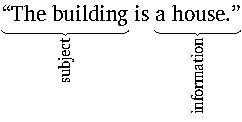
\includegraphics{A-Learners-Grammar-of-Classical-Standard-Arabic_files/figure-latex/unnamed-chunk-6-1.pdf}

The subject of the sentence is \enquote{the building}. This means that the sentence is about \enquote{the building}.

The information is \enquote{a house}. This means that the information that the sentence is giving us about the subject is that it is \enquote{a house}.

Let's try to form this sentence in Arabic.

First we assemble the individual parts:

\begin{enumerate}
\def\labelenumi{\roman{enumi}.}
\tightlist
\item
  \enquote{The building} in Arabic is \foreignlanguage{arabic}{ٱَلْبِنَاء} \emph{ʾalbināʾ} (masc.).
\item
  \enquote{A house} is \foreignlanguage{arabic}{بَيْت} \emph{bayt} (masc.).
\end{enumerate}

Next we put them both in the u-state. For subject-information sentences, both the subject and the information shall be in the u-state. Remember that the u-state is formed by putting a nūnated \emph{u}-mark \foreignlanguage{arabic}{◌ٌ} at the end of an indefinite noun, and a \emph{u}-mark \foreignlanguage{arabic}{◌ُ} at the end of a definite noun. Here are the two nouns in the u-state:

\begin{enumerate}
\def\labelenumi{\roman{enumi}.}
\tightlist
\item
  \foreignlanguage{arabic}{ٱَلْبِنَاءُ} \emph{ʾalbināʾu} (masc.) \enquote{the building} (u-state)
\item
  \foreignlanguage{arabic}{بَيْتٌ} \emph{baytun} (masc.) \enquote{a house} (u-state)
\end{enumerate}

In order to form this sentence in Arabic, we put the subject first and then the information. So we get:

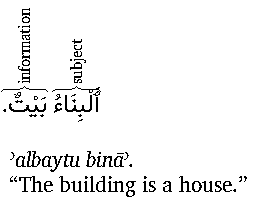
\includegraphics{A-Learners-Grammar-of-Classical-Standard-Arabic_files/figure-latex/unnamed-chunk-7-1.pdf}

But wait! Where is the Arabic word for \enquote{is}? It turns out that Arabic does not usually express any word for \enquote{is}. Instead, the meaning of this word is implied.

Also, note that the final vowel mark at the end of the sentence is written but not pronounced. So we will write
\foreignlanguage{arabic}{بَيْتٌ} but say
\emph{bayt}, not
\emph{baytun}.
This is in accordance with what we learned in section~\ref{pronouncing-the-end-of-a-sentence}.

Now let's try reversing this sentence, and try making the sentence:

\enquote{The house is a building.}

We follow the same procedure by assembling the individual parts of the sentence and putting them in the u-state:

\begin{enumerate}
\def\labelenumi{\roman{enumi}.}
\tightlist
\item
  The subject: \foreignlanguage{arabic}{ٱَلْبَيْتُ} \emph{ʾalbaytu} (masc.) \enquote{the house} (u-state)
\item
  The information: \foreignlanguage{arabic}{بِنَاءٌ} \emph{bināʾun} (masc.) \enquote{a building} (u-state)
\end{enumerate}

And then we put them together, first the subject and then the information:

\foreignlanguage{arabic}{ٱَلْبَيْتُ بِنَاءٌ.}\\
\emph{ʾalbaytu bināʾ.}\\
\enquote{The house is a building.}

and there we have our sentence.

\section{Matching the gender between the subject and the information}\label{matching-the-gender-between-the-subject-and-the-information}

In the sentences above, both the subject and the information were masculine nouns. Now let's try forming a sentence where the subject and the information have different genders. Let's try saying:

\enquote{The building is a school.}

\begin{enumerate}
\def\labelenumi{\roman{enumi}.}
\tightlist
\item
  The subject: \foreignlanguage{arabic}{ٱَلْبِنَاءُ} \emph{ʾalbināʾu} (masc.) \enquote{the building} (u-state)
\item
  The information: \foreignlanguage{arabic}{مَدْرَسَةٌ} \emph{madrasatun} (fem.) \enquote{a school} (u-state)
\end{enumerate}

In the same manner as before, we form the sentence by first writing the subject and then the information:

\foreignlanguage{arabic}{ٱَلْبِنَاءُ مَدْرَسَةٌ.}\\
\emph{ʾalbināʾu madrasah.}\\
\enquote{The building is a school.}

We can also reverse this sentence:

\foreignlanguage{arabic}{ٱَلْمَدْرَسَةُ بِنَاءٌ.}\\
\emph{ʾalmadrasatu bināʾ.}\\
\enquote{The school is a building .}

So we see that it is quite normal to have a sentence where the gender of the subject does not match the gender of the information.
This is because the words we have dealt with so far denote animate objects.
If either the subject or the information denote animate beings, then in this case the subject and the information often do match each other in gender. For example, let's try to form the sentence:

\enquote{The mother is a teacher.}

Here are the indiviual words that we will use to form the sentence:

\begin{enumerate}
\def\labelenumi{\roman{enumi}.}
\item
  The subject: \enquote{the mother}: \foreignlanguage{arabic}{ٱَلْأُمُّ} \emph{ʾalʾummu} (fem.) (u-state).
\item
  The information: \enquote{a teacher}. We have two words for \enquote{a teacher} in Arabic:

  \begin{itemize}
  \tightlist
  \item
    \foreignlanguage{arabic}{مُعَلِّم} \emph{muɛallium} (masc.) \enquote{a (male) teacher}
  \item
    \foreignlanguage{arabic}{مُعَلِّمَة} \emph{muɛallimah} (fem.) \enquote{a (female) teacher}.
  \end{itemize}

  Obviously, \foreignlanguage{arabic}{مُعَلِّمَة} \emph{muɛallimah} would apply here so we put it in the u-state: \foreignlanguage{arabic}{مُعَلِّمَةٌ} \emph{muɛallimatun}
  (u-state).
\end{enumerate}

Now we can assemble the sentence:

\foreignlanguage{arabic}{ٱَلْأُمُّ مُعَلِّمَةٌ.}\\
\emph{ʾalʾummu muɛallimah.}\\
\enquote{The mother is a teacher\textsubscript{f}.}

In the reverse sentence \enquote{The teacher is a mother.}, we again use the feminine noun
\foreignlanguage{arabic}{مُعَلِّمَة} \emph{muɛallimah} (fem.) \enquote{a (female) teacher},
which is now the subject of the sentence, to match the feminine noun in the information
\foreignlanguage{arabic}{ٱَلْأُمّ} \emph{ʾalumm} (fem.)
\enquote{a mother}. So we get:

\foreignlanguage{arabic}{ٱَلْمُعَلِّمَةُ أُمٌّ.}\\
\emph{ʾalmuɛallimatu ʾumm.}\\
\enquote{The teacher\textsubscript{f} is a mother.}

Here is another example:

\foreignlanguage{arabic}{ٱَلرَّجُلُ أَبٌ.}\\
\emph{ʾarrujulu ʾab.}\\
\enquote{The man is a father.}

Now, let's try a sentence where we are still dealing with animate beings but the nouns mismatches in grammatical gender.

\foreignlanguage{arabic}{ٱَلْأُمُّ شَخْصٌ.}\\
\emph{ʾalʾummu s͡hak͡hṣ.}\\
\enquote{The mother is a person.}

\foreignlanguage{arabic}{ٱَلشَّخْصُ مُعَلِّمَةٌ.}\\
\emph{ʾas͡hs͡hak͡hṣu muɛallimah.}\\
\enquote{The person is a (female) teacher.}

\foreignlanguage{arabic}{ٱَلْمُعَلِّمَةُ شَخْصٌ.}\\
\emph{ʾalmuɛallimatu s͡hak͡hṣ.}\\
\enquote{The (female) teacher is a person.}

In the above examples, the grammatical genders mismatch between the subject and the information. But this is because we are matching with the physical gender of the person represented by the masculine noun \foreignlanguage{arabic}{شَخْص} \emph{s͡hak͡hṣ} \enquote{a person}, not its grammatical gender.

The same effect is seen when using the word \foreignlanguage{arabic}{حَيَوان} \emph{ḥayawān} which is a masculine noun meaning \enquote{an animal}. It can be applied to both male and female animals. So we can say:

\foreignlanguage{arabic}{ٱَلْحَيَوَانُ هِرٌّ.}\\
\emph{ʾalḥayawānu hirr.}\\
\enquote{The animal is a (male) cat.}

and

\foreignlanguage{arabic}{ٱَلْحَيَوَانُ هِرَّةٌ.}\\
\emph{ʾalḥayawānu hirrah.}\\
\enquote{The animal is a (female) cat.}

\section{Detached pronouns}\label{detached-pronouns}

Pronouns, in Arabic, are special nouns that can be used in place of other nouns when it is known who is being referred to. This means that they can replace definite nouns only. Pronouns in English include words like \enquote{he}, \enquote{she}, \enquote{it}, \enquote{you}, \enquote{I}, etc.

In order to explain the usage of pronouns, we will first show a sentence with a noun subject:

\enquote{The man is a teacher.}

Now we you can replace the definite subject noun \enquote{the man} with the pronoun \enquote{he}:

\enquote{He is a teacher.}

In Arabic there are a few different kinds of pronouns. Here we will learn \emph{detached pronouns}. They are called detached pronouns because they are detached from other words. There are another set of pronouns called \emph{attached pronouns} that we will learn later, if Allāh wills.

\subsection{Participants}\label{participants}

When talking about pronouns, it is beneficial to make use of a concept of grammar called \emph{participants}.

In any kind of speech there are there can be up to three types of \emph{participants} involved. A participant may be singular, i.e.~consist of one individual, or plural, i.e., consist of more than one individual.

The three participants in speech are:

\begin{enumerate}
\def\labelenumi{\arabic{enumi}.}
\tightlist
\item
  The \emph{speaker-participant}. This is the participant who is speaking. When the speaker-participant refers to himself or herself (or themselves if plural) in English, then he/she/they use the pronouns \enquote{I}, \enquote{me}, \enquote{we}, and \enquote{us}.
\item
  The \emph{addressee-participant}. This is the participant whom the speaker-participant is directly speaking to. When the speaker-participant refers to the addressee-participant in English, he uses the \enquote{you} pronoun.
\item
  The \emph{absentee-participant}. This is the participant who is not being directly spoken to. Their only participation in the speech is that they are being referred to. When the speaker-participant refers to the absentee-participant in English, he uses the pronouns \enquote{he}, \enquote{him}, \enquote{she}, \enquote{her}, \enquote{it}, \enquote{they}, and \enquote{them}.
\end{enumerate}

In this chapter we will learn the Arabic pronouns for the singular participants.

\subsection{Detached pronouns for the singular absentee-participant}\label{detached-pronouns-for-the-singular-absentee-participant}

Here are the Arabic detached pronouns for the singular absentee-participant:

\begin{itemize}
\tightlist
\item
  singular masculine absentee-participant: \foreignlanguage{arabic}{هُوَ} \emph{huwa} \enquote{he}.
\item
  singular feminine absentee-participant: \foreignlanguage{arabic}{هِيَ} \emph{hiya} \enquote{she}.
\end{itemize}

Here are some examples of pair of sentences, each first with a noun, and then with a pronoun in place of the noun:

\begin{itemize}
\item
  \foreignlanguage{arabic}{ٱَلرَّجُلُ مُعَلِّمٌ.}\\
  \emph{ʾarrajulu muɛallim.}\\
  \enquote{The man is a teacher\textsubscript{m}.}

  \foreignlanguage{arabic}{هُوَ مُعَلِّمٌ.}\\
  \emph{huwa muɛallim.}\\
  \enquote{He is a (male) teacher\textsubscript{m}.}
\item
  \foreignlanguage{arabic}{ٱَلْجَارِيَةُ طَالِبَةٌ.}\\
  \emph{ʾaljāriyatu ṭalibah.}\\
  \enquote{The girl is a student\textsubscript{f}.}
\item
  \foreignlanguage{arabic}{هِيَ طَالِبَةٌ.}\\
  \emph{hiya ṭalibah.}\\
  \enquote{She is a student\textsubscript{f}.}
\item
  \foreignlanguage{arabic}{ٱَلْبَيْتُ بِنَاءٌ.}\\
  \emph{ʾalbaytu bināʾ.}\\
  \enquote{The house is a building.}

  \foreignlanguage{arabic}{هُوَ بِنَاءٌ.}\\
  \emph{huwa bināʾ.}\\
  \enquote{It is a building.}

  Note that Arabic uses the pronoun \foreignlanguage{arabic}{هُوَ} \emph{huwa} \enquote{he} to refer to the inanimate object \enquote{the house}. This is because, as we know, all nouns in Arabic are either masculine or feminine. In translating the sentence to English we will employ the neutral pronoun \enquote{it} to make the sentence sound natural.
\item
  \foreignlanguage{arabic}{ٱَلْبِنَاءُ مَدْرَسَةٌ.}\\
  \emph{ʾalbināʾu madrasah.}\\
  \enquote{The building is a school.}

  \foreignlanguage{arabic}{هُوَ مَدْرَسَةٌ.}
  \emph{huwa madrasah.}\\
  or\\
  \foreignlanguage{arabic}{هِيَ مَدْرَسَةٌ.}
  \emph{hiya madrasah.}\\
  \enquote{It is a school.}

  Note that either \foreignlanguage{arabic}{هُوَ} \emph{huwa} \enquote{he} or \foreignlanguage{arabic}{هِيَ} \emph{hiya} \enquote{she} can be used in the above sentence because the gender of the subject \foreignlanguage{arabic}{ٱَلْبِنَاء} \emph{ʾalbināʾ} (masc.) \enquote{the building} mismatches the gender of the information \foreignlanguage{arabic}{مَدْرَسَة} \emph{madrasah} (fem.) \enquote{a school.}.

  In such cases where the genders of the subject and the information do not match, then, generally speaking, the pronoun for either gender could be employed with the following guideline:

  Prefer to match the gender of the subject pronoun with the gender of the information, unless the noun being replaced with a pronoun is an animate being, in which case prefer to use the gender of the animate being.

  So in the above sentence we will prefer to use \foreignlanguage{arabic}{هِيَ مَدْرَسَةٌ.} \emph{hiya madrasah.} because the information \foreignlanguage{arabic}{مَدْرَسَةٌ} \emph{madrasatun} \enquote{a school} is feminine.
\item
  Here is an example with an animate being as the subject:

  \foreignlanguage{arabic}{ٱَلْجَارِيَةُ إِنْسَانٌ.}\\
  \emph{ʾaljāriyatu īnsān.}\\
  \enquote{The girl is a human.}

  \foreignlanguage{arabic}{هِيَ إِنْسَانٌ.}\\
  \emph{hiya īnsān.}\\
  \enquote{She is a human.}

  Here, if we replace the noun \foreignlanguage{arabic}{ٱَلْجَارِيَة} \emph{ʾaljāriyah} \enquote{the girl} with a pronoun, we will prefer to use \foreignlanguage{arabic}{هِيَ} \emph{hiya} \enquote{she}, because the girl is an animate being, even though the information \foreignlanguage{arabic}{إِنْسَانٌ} \emph{ʾinsānun} \enquote{a human} is masculine.
\end{itemize}

\subsection{Detached pronouns for the singular addressee-participant and speaker-participant}\label{detached-pronouns-for-the-singular-addressee-participant-and-speaker-participant}

Here are the pronouns for the singular addressee-participant and speaker-participant:

\begin{itemize}
\tightlist
\item
  singular masculine addressee-participant: \foreignlanguage{arabic}{أَنْتَ} \emph{ʾanta} \enquote{you\textsubscript{m}}.
\item
  singular feminine addressee-participant: \foreignlanguage{arabic}{أَنْتِ} \emph{ʾanti} \enquote{you\textsubscript{f}}.
\item
  singular speaker-participant: \foreignlanguage{arabic}{أَنَا} \emph{ʾana} \enquote{I}.
\end{itemize}

Note that the addressee-participant pronoun \enquote{you} has separate pronouns for the masculine and the feminine while the speaker-participant pronoun \enquote{I} has the same pronoun for both genders. Examples with these pronouns:

\begin{itemize}
\item
  \foreignlanguage{arabic}{أَنْتَ مُعَلِّمٌ.}\\
  \emph{ʾanta muɛallim.}\\
  \enquote{You\textsubscript{m} are a teacher\textsubscript{m}.}
\item
  \foreignlanguage{arabic}{أَنْتِ مُعَلِّمَةٌ.}\\
  \emph{ʾanti muɛallimah.}\\
  \enquote{You\textsubscript{f} are a teacher\textsubscript{f}.}
\item
  \foreignlanguage{arabic}{أَنَا مُعَلِّمٌ.}\\
  \emph{ʾana muɛallim.}\\
  \enquote{I am a teacher\textsubscript{m}.}
\item
  \foreignlanguage{arabic}{أَنَا مُعَلِّمَة.}\\
  \emph{ʾana muɛallimah.}\\
  \enquote{I am a teacher\textsubscript{f}.}
\end{itemize}

\subsection{Definiteness of pronouns}\label{definiteness-of-pronouns}

We stated, and saw, that pronouns can replace definite nouns. This means that pronouns themselves are definite nouns (even though they are not prefixed by \foreignlanguage{arabic}{ٱَلْ} \emph{ʾal} \enquote{the}).

This fact will be useful in later chapters, if Allāh wills.

\subsection{Rigidity of pronouns}\label{rigidity-of-pronouns}

Remember in section~\ref{flexibility-of-nouns}, we talked about the flexibility of nouns. We said that nouns whose endings change with the noun's state are called flexible nouns. Most nouns fall into this category.

Pronouns, however, are nouns whose endings don't change with their state. Therefore they fall into the category of \emph{rigid} nouns.

\section{A definite noun as the information}\label{chap-smp-sent-sec-def-info}

In all the examples so far, the information has been an indefinite noun: \enquote{a building}, \enquote{a teacher}, \enquote{a cat}, etc. It is also possible for the information to be a definite noun:

\foreignlanguage{arabic}{ٱَلرَّجُلُ ٱلْمُعَلِّمُ.}\\
\emph{ʾarrajulu -lmuɛallim.}\\
\enquote{The man is the teacher\textsubscript{m}.}

The above sentence, although correct, is ambiguous. It can also be interpreted as a noun-phrase, meaning \enquote{the teacher-man}, instead of the complete sentence \enquote{The man is the teacher\textsubscript{m}.} Therefore, in order to disambiguate and make it clear that we mean the complete sentence, a \emph{disambiguating pronoun} is usually (but not always) inserted between the subject and the information.
Disambiguating pronouns are detached pronouns that match the subject of the sentence in gender. With a disambiguating pronoun, the sentence above becomes:

\foreignlanguage{arabic}{ٱَلرَّجُلُ هُوَ ٱلْمُعَلِّمُ.}\\
\emph{ʾarrajulu huwa -lmuɛallim.}\\
\enquote{The man is the teacher\textsubscript{m}.}

The disambiguating pronoun here is \foreignlanguage{arabic}{هُوَ} \emph{huwa} and is not translated. Here are some more examples of sentences with definite informations and disambiguating pronouns.

\foreignlanguage{arabic}{ٱَلْبَيْتُ هُوَ ٱلْبِنَاءُ.}\\
\emph{ʾalbaytu -lbināʾu.}\\
\enquote{The house is the building.}

\foreignlanguage{arabic}{ٱَلْحَيَوَانُ هِيَ ٱلْهِرَّةُ.}\\
\emph{ʾalḥayawānu hiya -lhirratu.}\\
\enquote{The animal is the cat.}

\section{An indefinite noun as the subject}\label{an-indefinite-noun-as-the-subject}

In all the sentences we have seen so far, the subject has always been a definite noun. This is usually the case. A subject needs a certain amount of \emph{weight} in order to be the first word in a sentence. And being definite gives it this needed weight. That is: \enquote{the man} is grammatically \emph{heavier} than \enquote{a man}. So it is easier to start a sentence with \enquote{the man}.

So can we even have a sentence that has an indefinite subject? For example:

\begin{itemize}
\tightlist
\item
  A house is a building.
\item
  A man is the teacher.
\end{itemize}

Yes, it is possible, but sentences where the subject is an indefinite noun are not as straightforward to express in Arabic. We will explore some ways of expressing them later if Allāh wills.

\section{\texorpdfstring{\foreignlanguage{arabic}{وَ} \emph{wa-} \enquote{and}, \foreignlanguage{arabic}{فَ} \emph{fa-} \enquote{so}/\enquote{and then}, and \foreignlanguage{arabic}{أَوْ} \emph{ʾaw} \enquote{or}}{وَ wa- ``and'', فَ fa- ``so''/``and then'', and أَوْ ʾaw ``or''}}\label{ux648-wa--and-ux641-fa--soand-then-and-ux623ux648-eaw-or}

\subsection{\texorpdfstring{\foreignlanguage{arabic}{وَ} \emph{wa-} \enquote{and}}{وَ wa- ``and''}}\label{ux648-wa--and}

Arabic uses the particle \foreignlanguage{arabic}{وَ} \emph{wa} to mean \enquote{and}. Being a one-letter particle, it is joined to the word after it without any space between it and the next word.

\foreignlanguage{arabic}{وَمَدْرَسَةٌ}\\
\emph{wamadrasatun}\\
\enquote{and a school}

\foreignlanguage{arabic}{وَ} \emph{wa} meaning \enquote{and} does not change the state of the noun following it. Examples:

\foreignlanguage{arabic}{ٱَلْبِنَاءُ مَسْجِدٌ وَمَدْرَسَةٌ.}\\
\emph{ʾalbināʾu masjidun wamadrasah.}\\
\enquote{The building is a mosque and a school.}

If there are more than two words, then in English, only the final word usually has \enquote{and} and the rest are separated by commas in writing. In Arabic, however, each must have \foreignlanguage{arabic}{وَ} and commas are not typically used.

\foreignlanguage{arabic}{ٱَلْبِنَاءُ مَسْجِدٌ وَمَدْرَسَةٌ وَمَکْتَبَةٌ.}\\
\emph{ʾalbināʾu baytun wamadrasatun wamaktabah}\\
\enquote{The building is a mosque, a school, and a library.}

We can also use \foreignlanguage{arabic}{وَ} to begin and connect sentences. The following example is tehcnically two sentences, both beginning with \foreignlanguage{arabic}{وَ}:

\foreignlanguage{arabic}{وَٱلرَّجُلُ إِنْسَانٌ وَٱلْکَلْبُ حَيَوَانٌ}\\
\emph{warrujulu ʾinṣānun wa-lkalbu ḥayawānun}\\
\enquote{And the man is a human and the dog is an animal.}

Unlike as in English, this is not considered poor style. When translating such sentences to English, the first \foreignlanguage{arabic}{وَ} is often left out, thus:
\enquote{The man is a human and the dog is an animal.}

\subsection{\texorpdfstring{\foreignlanguage{arabic}{فَ} \emph{fa-} \enquote{so}/\enquote{and then}}{فَ fa- ``so''/``and then''}}\label{ux641-fa--soand-then}

The word \foreignlanguage{arabic}{فَ} \emph{fa-} \enquote{so}/\enquote{and then} is comparable to \foreignlanguage{arabic}{وَ} \emph{wa-} \enquote{and}.
\foreignlanguage{arabic}{فَ} \emph{fa-} \enquote{so}/\enquote{and then}
gives a meaning of ordering, consequence, and subsequence that is missing in \foreignlanguage{arabic}{وَ} \emph{wa-} \enquote{and}. For example,

\foreignlanguage{arabic}{ٱَلْبِنَاءُ مَسْجِدٌ فَمَدْرَسَةٌ فَمَکْتَبَةٌ.}\\
\emph{ʾalbināʾu baytun famadrasatun famaktabah}\\
\enquote{The building is a mosque, and then a school, and then a library.}

\foreignlanguage{arabic}{فَ} \emph{fa-} \enquote{so}/\enquote{and then}, too, is used to begin and connect sentences. Example,

\foreignlanguage{arabic}{فَٱلرَّجُلُ إِنْسَانٌ وَٱلْکَلْبُ حَيَوَانٌ}\\
\emph{farrujulu ʾinṣānun wa-lkalbu ḥayawānun}\\
\enquote{So the man is a human and the dog is an animal.}

\chapter{Prepositions}\label{prepositions}

\section{Introduction}\label{introduction-3}

Prepositions are words like \enquote{in}, \enquote{on}, \enquote{from}, etc. They are placed directly before a noun, for example: \enquote{in a house}. The preposition \enquote{in} is placed directly before the noun \enquote{a house}.

In Arabic prepositions, when placed before a noun, put it in the i-state. For example the preposition \foreignlanguage{arabic}{فِي} \emph{fī} means \enquote{in}. We can put it before the noun \foreignlanguage{arabic}{بَيْت} \emph{bayt} \enquote{a house}:

\foreignlanguage{arabic}{فِي بَيْتٍ}\\
\emph{fī baytin}\\
\enquote{in a house}

Note how the noun \foreignlanguage{arabic}{بَيْتٍ} \emph{baytin} \enquote{a house} is in the i-state because of the preposition \foreignlanguage{arabic}{فِي} \emph{fī} \enquote{in} before it. The i-state is indicated by the nūnated \emph{i}-mark \foreignlanguage{arabic}{◌ٍ} on the final letter of \foreignlanguage{arabic}{بَيْت}.

Arabic has two types of prepositions: \emph{true} prepositions and \emph{pseudo}-prepositions.

\section{True prepositions}\label{true-prepositions}

True prepositions are \emph{particles}. Particles are a class of words, like nouns and verbs. Particles don't have the properties of nouns. Thus, they cannot be definite or indefinite. They cannot be preceded by \foreignlanguage{arabic}{ٱَلْ} \emph{al} nor may they be nūnated. And they don't have state (u-state, a-state, i-state).

Here is a list of the more common true prepositions:

\begin{longtable}[]{@{}ll@{}}
\toprule\noalign{}
Preposition & Meaning \\
\midrule\noalign{}
\endhead
\bottomrule\noalign{}
\endlastfoot
\foreignlanguage{arabic}{بِ} \emph{bi} & with, by, next to \\
\foreignlanguage{arabic}{لِ} \emph{li} & for, to \\
\foreignlanguage{arabic}{فِي} \emph{fī} & in \\
\foreignlanguage{arabic}{عَلَىٰ} \emph{ɛalā} & on \\
\foreignlanguage{arabic}{إِلَىٰ} \emph{ʾilā} & to, toward \\
\foreignlanguage{arabic}{مِنْ} \emph{min} & from \\
\foreignlanguage{arabic}{عَنْ} \emph{ɛan} & from, about \\
\foreignlanguage{arabic}{کَ} \emph{ka} & like \\
\end{longtable}

Notes:

\begin{itemize}
\item
  Prepositions that are a single letter (like
  \foreignlanguage{arabic}{بِ} \emph{bi}, \foreignlanguage{arabic}{ل} \emph{li}, \foreignlanguage{arabic}{کَ} \emph{ka}) are joined to the following noun in writing. Example:

  \foreignlanguage{arabic}{بِقَلَمٍ}\\
  \emph{biqalamin}\\
  \enquote{with a pen}

  \foreignlanguage{arabic}{لِرَجُلٍ}\\
  \emph{lirajulin}\\
  \enquote{for a man}

  \foreignlanguage{arabic}{کَٱبْنٍ}\\
  \emph{ka-bnin}\\
  \enquote{like a son}
\item
  When a single letter preposition comes before a definite noun with \foreignlanguage{arabic}{ٱَلْ} \emph{al}, the preposition is generally joined to the \foreignlanguage{arabic}{أَلِف} in the \foreignlanguage{arabic}{ٱَلْ} \emph{al}. The \foreignlanguage{arabic}{أَلِف} is now not pronounced (because as we know it has a connecting hamzah). Example:

  \foreignlanguage{arabic}{بِٱلْقَلَمِ}\\
  \emph{bi-lqalami}\\
  \enquote{with the pen}

  If the noun begins with a connecting hamzah then the \foreignlanguage{arabic}{ل} in \foreignlanguage{arabic}{ٱَلْ} gets an \emph{i}-mark \foreignlanguage{arabic}{◌ِ} instead of its usual ø-mark \foreignlanguage{arabic}{◌ْ}. We described this in
  section~\ref{the-definite-article-with-nouns-with-an-initial-connecting-hamzah}.
  Example:

  \foreignlanguage{arabic}{کَٱلِٱبْنِ}\\
  \emph{ka-li-bni}\\
  \enquote{like the son}
\item
  The only exception is the preposition \foreignlanguage{arabic}{لِ} \emph{li}. When joined to a definite noun with \foreignlanguage{arabic}{ٱَلْ} \emph{al}, the \foreignlanguage{arabic}{أَلِف} in \foreignlanguage{arabic}{ٱَلْ} is dropped and we write the two \emph{lām}s together. Example:

  \foreignlanguage{arabic}{لِلرَّجُلِ}\\
  \emph{li-rrajuli}\\
  \enquote{for the man}

  \foreignlanguage{arabic}{لِلْجَارِيَةِ}\\
  \emph{li-ljāriyati}\\
  \enquote{for the girl}

  \foreignlanguage{arabic}{لِلِٱبْنِ}\\
  \emph{li-li-bni}\\
  \enquote{for the son}

  However, in this case, if the noun too starts with a \emph{lām}, then we drop the entire \foreignlanguage{arabic}{ٱَلْ} \emph{al} (in writing, not in meaning). This is to avoid having three \emph{lām}s joined to each other. Example:

  \foreignlanguage{arabic}{ٱَللُّعْبَةُ}\\
  \emph{ʾalluɛbatu}\\
  \enquote{the toy}

  becomes

  \foreignlanguage{arabic}{لِلُّعْبَةِ}\\
  \emph{li-lluɛbati}\\
  \enquote{for the toy}

  not

  \(\times\)~\foreignlanguage{arabic}{لِللُّعْبَةِ}

  This is also true for the phrase:

  \foreignlanguage{arabic}{لِلَّـٰهِ}\\
  \emph{lillāhi}\\
  \enquote{for Allāh}

  which is formed from \foreignlanguage{arabic}{لِ + ٱللَّـٰهِ}
\item
  The prepositions
  \foreignlanguage{arabic}{عَلَىٰ} \emph{ɛalā} \enquote{on} and
  \foreignlanguage{arabic}{إِلَىٰ} \emph{ʾilā} \enquote{to} have a long-\emph{ā} vowel at the end but it is written with a dotless yāʾ \foreignlanguage{arabic}{ىٰ} instead of an \foreignlanguage{arabic}{أَلِف}. (We have already learned that some words are written this way in section~\ref{a-vowel-written-with-a-ya}.)
\item
  Prepositions that are composed of multiple letters are not joined to the following noun. Example:

  \foreignlanguage{arabic}{إِلَىٰ مَدْرَسَةٍ}\\
  \emph{ʾilā madrasatin}\\
  \enquote{to a school}
\item
  If a preposition ends with a long vowel, then, as usual, it get shortened to a short vowel when it is followed by a word which begins with a connecting hamzah. Examples:

  \foreignlanguage{arabic}{فِي ٱلْبَيْتِ}\\
  \emph{fi -lbayti}\\
  \enquote{in the house}

  \foreignlanguage{arabic}{إِلَى ٱبْنٍ}\\
  \emph{ʾila -bnin}\\
  \enquote{to a son}
\item
  If a preposition ends with a ø-mark \foreignlanguage{arabic}{◌ْ} and it is followed by a word that begins with a connecting hamzah, then the ø-mark is changed to a short vowel according to the following rules:

  \begin{itemize}
  \item
    The ending of the preposition \foreignlanguage{arabic}{عَنْ} \emph{ɛan} gets an \emph{i}-mark and becomes \foreignlanguage{arabic}{عَنِ} \emph{ɛani}. Examples:

    \foreignlanguage{arabic}{عَنِ ٱلرَّجُلِ}\\
    \emph{ɛani -rrajuli}\\
    \enquote{from the man}

    \foreignlanguage{arabic}{عَنِ ٱبْنٍ}\\
    \emph{ɛani -bnin}\\
    \enquote{from the son}
  \item
    The ending of the preposition \foreignlanguage{arabic}{مِنْ} \emph{min} gets an \emph{a}-mark if followed by the \foreignlanguage{arabic}{ٱَلْ} \emph{al} of a definite noun. Otherwise it gets an \emph{i}-mark if followed by any other connecting hamzah. Examples:

    \foreignlanguage{arabic}{مِنَ ٱلرَّجُلِ}\\
    \emph{mina -rrajuli}\\
    \enquote{from the man}

    \foreignlanguage{arabic}{مِنِ ٱبْنٍ}\\
    \emph{mini -bnin}\\
    \enquote{from a son}
  \end{itemize}
\end{itemize}

\section{Pseudo-prepositions}\label{pseudo-prepositions}

Pseudo-prepositions are actually nouns but they are used as prepositions. The above rules of writing and pronunciation apply to them as well.

Here is a list of some common pseudo-prepositions:

\begin{longtable}[]{@{}lll@{}}
\toprule\noalign{}
Preposition & Transcription & Meaning \\
\midrule\noalign{}
\endhead
\bottomrule\noalign{}
\endlastfoot
\foreignlanguage{arabic}{عِنْدَ} & \emph{ɛinda} & at \\
\foreignlanguage{arabic}{لَدَىٰ} & \emph{ladā} & at \\
\foreignlanguage{arabic}{لَدُنْ} & \emph{ladun} & at \\
\foreignlanguage{arabic}{مَعَ} & \emph{maɛa} & together with \\
\foreignlanguage{arabic}{بَيْنَ} & \emph{bayna} & between, among \\
\end{longtable}

There are three different prepositions above that we have translated as \enquote{at}. \foreignlanguage{arabic}{لَدُنْ} is relatively rarer compared to the others. Otherwise, they are largely interchangeable but there are some differences in meaning that we will explain later, if Allāh wills.

Here are some examples using pseudo-prepositions:

\foreignlanguage{arabic}{مَعَ ٱلْغُلَامِ}\\
\emph{maɛa -lg͡hulāmi}\\
\enquote{with the boy}

\foreignlanguage{arabic}{عِنْدَ ٱلْبَيْتِ}\\
\emph{ɛinda -lbayti}\\
\enquote{at the house}

\foreignlanguage{arabic}{لَدَى ٱلْبَابِ}\\
\emph{lada -lbābi}\\
\enquote{at the door}

\foreignlanguage{arabic}{بَيْنَ ٱلنَّاسِ}\\
\emph{bayna -nnāsi}\\
\enquote{among the people}

\section{Attached pronouns}\label{attached-pronouns}

We have already learned detached pronouns \foreignlanguage{arabic}{هُوَ}, \foreignlanguage{arabic}{هِيَ}, and \foreignlanguage{arabic}{أَنَا} in section~\ref{detached-pronouns}.
Detached pronouns are the equivalent of \enquote{he}, \enquote{she}, and \enquote{I}, etc. They are used in place of nouns that are in the u-state.

Now we will learn about \emph{attached pronouns}. Attached pronouns are, more or less, the equivalent of \enquote{him}, \enquote{her}, and \enquote{me}, etc.
They are used in place of nouns that are in the a-state and the i-state. One place where attached pronouns are used is when the replace the noun directly following a preposition.

The singular attached pronouns are listed below. The detached pronouns are included as well for easy comparison.

\begin{longtable}[]{@{}
  >{\raggedright\arraybackslash}p{(\columnwidth - 4\tabcolsep) * \real{0.4118}}
  >{\raggedright\arraybackslash}p{(\columnwidth - 4\tabcolsep) * \real{0.2941}}
  >{\raggedright\arraybackslash}p{(\columnwidth - 4\tabcolsep) * \real{0.2941}}@{}}
\toprule\noalign{}
\begin{minipage}[b]{\linewidth}\raggedright
Participant
\end{minipage} & \begin{minipage}[b]{\linewidth}\raggedright
Detached pronoun
\end{minipage} & \begin{minipage}[b]{\linewidth}\raggedright
Attached pronoun
\end{minipage} \\
\midrule\noalign{}
\endhead
\bottomrule\noalign{}
\endlastfoot
Masc. absentee & \foreignlanguage{arabic}{هُوَ} \emph{huwa} \enquote{him} & \foreignlanguage{arabic}{هُ} \emph{-hu} \enquote{him} \\
Fem. absentee & \foreignlanguage{arabic}{هِيَ} \emph{hiya} \enquote{her} & \foreignlanguage{arabic}{هَا} \emph{-hā} \enquote{her} \\
Masc. addressee & \foreignlanguage{arabic}{أَنْتَ} \emph{ʾanta} \enquote{you\textsubscript{1,m}} & \foreignlanguage{arabic}{کَ} \emph{-ka} \enquote{you\textsubscript{1,m}} \\
Fem. addressee & \foreignlanguage{arabic}{أَنْتِ} \emph{ʾanti} \enquote{you\textsubscript{1,f}} & \foreignlanguage{arabic}{کِ} \emph{-ki} \enquote{you\textsubscript{1,f}} \\
Speaker & \foreignlanguage{arabic}{أَنَا} \emph{ʾana} \enquote{I} & \foreignlanguage{arabic}{ي} \enquote{me} \\
\end{longtable}

\subsection{Attached pronouns with prepositions}\label{attached-pronouns-with-prepositions}

As mentioned above, one place the attached pronouns are used are after prepositions.
Here are some notes regarding how they attach to prepositions:

\begin{enumerate}
\def\labelenumi{\arabic{enumi}.}
\item
  Generally, these pronouns attach to the last letter of the preposition before it. Examples:

  \begin{itemize}
  \tightlist
  \item
    \foreignlanguage{arabic}{مِنْکَ} \emph{minka} \enquote{from you}
  \item
    \foreignlanguage{arabic}{مَعَهُ} \emph{maɛahu} \enquote{with him}
  \item
    \foreignlanguage{arabic}{عَنْهَا} \emph{ɛanhā} \enquote{from her}
  \end{itemize}
\item
  The \foreignlanguage{arabic}{ىٰ} \emph{ā} ending of prepositions become \foreignlanguage{arabic}{◌َيْ} \emph{-ay} when attaching an attached pronoun. Examples:

  \begin{itemize}
  \tightlist
  \item
    \foreignlanguage{arabic}{إِلَيْهَا} \emph{ʾilayhā} \enquote{to her}
  \item
    \foreignlanguage{arabic}{عَلَيْکَ} \emph{ɛalayka} \enquote{on you\textsubscript{m}}
  \end{itemize}
\item
  The pronoun \foreignlanguage{arabic}{هُ} \emph{-hu} \enquote{him} becomes \foreignlanguage{arabic}{هِ} \emph{hi} when it is preceded by the vowels \foreignlanguage{arabic}{◌ِ} \emph{-i}, \foreignlanguage{arabic}{◌ِي} \emph{-ī}, or the semi-vowel \foreignlanguage{arabic}{◌َيْ} \emph{-ay}. So we get

  \begin{itemize}
  \tightlist
  \item
    \foreignlanguage{arabic}{بِهِ} \emph{bihi} \enquote{with him}
  \item
    \foreignlanguage{arabic}{فِيهِ} \emph{fīhi} \enquote{in him}
  \item
    \foreignlanguage{arabic}{إِلَيْهِ} \emph{ʾilayhi} \enquote{to him}
  \end{itemize}
\item
  The attached pronoun for the speaker deserves special attention. The pronoun itself is the letter \foreignlanguage{arabic}{ي}. But it has two variants:

  \begin{enumerate}
  \def\labelenumii{\roman{enumii}.}
  \tightlist
  \item
    \foreignlanguage{arabic}{◌ِي} \emph{-ī}
  \item
    \foreignlanguage{arabic}{◌ِيَ} \emph{-iya}
  \end{enumerate}

  Generally, both of these variants cause the final letter of the word before them, if a consonant, to have an \emph{i}-mark \foreignlanguage{arabic}{◌ِ}, regardless of the whether or not that letter originally had an \emph{i}-mark. Examples:

  \begin{itemize}
  \tightlist
  \item
    \foreignlanguage{arabic}{لِي} \emph{lī} and \foreignlanguage{arabic}{لِيَ} \emph{liya} \enquote{for me}
  \item
    \foreignlanguage{arabic}{بِي} \emph{bī} and \foreignlanguage{arabic}{بِي} \emph{biya} \enquote{with/by me}
  \item
    \foreignlanguage{arabic}{مَعِي} \emph{maɛī} and \foreignlanguage{arabic}{مَعِيَ} \emph{maɛiya} \enquote{together with me}
  \item
    \foreignlanguage{arabic}{عِنْدِي} \emph{ɛindī} and \foreignlanguage{arabic}{عِنْدِيَ} \emph{ɛindiya} \enquote{at me}
  \end{itemize}

  Between these two, variants, \foreignlanguage{arabic}{◌ِي} \emph{-ī} is more commonly used generally, except in the cases described in the next point, below:
\item
  For any word that ends with a long vowel (\emph{-ā}, \emph{-ī}, or \emph{-ū}) or a semi-vowel (\emph{-ay} or \emph{-aw}), the variant \foreignlanguage{arabic}{◌ِي} \emph{-ī} for the speaker attached pronoun is not used. Instead, only the variant \foreignlanguage{arabic}{يَ} \emph{-ya} may be used with such words.

  Prepositions that fall under this category are \foreignlanguage{arabic}{فِي} \emph{fī}, \foreignlanguage{arabic}{عَلَىٰ} \emph{ɛalā}, \foreignlanguage{arabic}{إِلَىٰ} \emph{ʾilā}, and \foreignlanguage{arabic}{لَدَىٰ} \emph{ladā}. Furthermore, the \foreignlanguage{arabic}{ىٰ} \emph{-ā} ending in these will become \foreignlanguage{arabic}{◌َيْ} \emph{ay} instead when attaching the pronoun.

  In addition, the pronoun \foreignlanguage{arabic}{يَ} \emph{-ya} will not cause the final letter of word before it to have an \emph{i}-mark because it does that only to consonants, not to vowels or semivowels.

  So we get:

  \begin{itemize}
  \tightlist
  \item
    \foreignlanguage{arabic}{يَ} + \foreignlanguage{arabic}{فِي} = \foreignlanguage{arabic}{فِيَّ} \emph{fiyya} \enquote{in me}
  \item
    \foreignlanguage{arabic}{يَ} + \foreignlanguage{arabic}{إِلَيْ} = \foreignlanguage{arabic}{إِلَيَّ} \emph{ʾilayya} \enquote{to me}
  \item
    \foreignlanguage{arabic}{يَ} + \foreignlanguage{arabic}{عَلَيْ} = \foreignlanguage{arabic}{عَلَيَّ} \emph{ɛalayya} \enquote{on me}
  \item
    \foreignlanguage{arabic}{يَ} + \foreignlanguage{arabic}{لَدَيْ} = \foreignlanguage{arabic}{لَدَيَّ} \emph{ladayya} \enquote{at me}.
  \end{itemize}
\item
  The preposition \foreignlanguage{arabic}{کَ} \emph{ka} \enquote{like} is not used with any attached pronoun. So, for example, we don't say:

  \begin{itemize}
  \tightlist
  \item
    \(\times\)~\foreignlanguage{arabic}{کَهُ} \emph{kahu} for \enquote{like him.}
  \end{itemize}

  Instead, we will learn another method to express this meaning in later chapters, if Allāh wills.
\item
  The word \enquote{between}, because of its meaning, is typically used with two or more individuals. For example, \enquote{between us}, \enquote{between you and him}, etc. In Arabic, when the pseudo-preposition \foreignlanguage{arabic}{بَيْنَ} \emph{bayna} is used with a singular attached pronoun, it is repeated. For example,

  \begin{itemize}
  \tightlist
  \item
    \foreignlanguage{arabic}{بَيْنِي وَبَيْنَکَ} \emph{baynī wabaynaka} \enquote{between me and you}
  \end{itemize}
\end{enumerate}

\section{Translating prepositions}\label{translating-prepositions}

For each preposition that we have listed above, we have also given its meaning. For example,

\begin{itemize}
\tightlist
\item
  \foreignlanguage{arabic}{فِي} \emph{fī} \enquote{in}
\item
  \foreignlanguage{arabic}{بِ} \emph{bi} \enquote{with}, \enquote{by}, \enquote{next to}
\end{itemize}

These meanings are not always fixed. And there is some degree of overlap in meanings as well. For example, in order to say \enquote{in the city} we will usually say
\foreignlanguage{arabic}{فِي ٱلْمَدِينَةِ} \emph{fi -lmadīnati} but sometimes we can also say
\foreignlanguage{arabic}{بِٱلْمَدِينَةِ} \emph{bi -lmadīnati} with the same meaning. As you keep learning, practicing, and reading Arabic, you will learn how to choose which preposition to use, if Allah wills.

Similarly, sometimes we have two or more prepositions with almost the same meaning. For example,

\begin{itemize}
\tightlist
\item
  \foreignlanguage{arabic}{مِنْ} \emph{min} \enquote{from}
\item
  \foreignlanguage{arabic}{عَنْ} \emph{ɛan} \enquote{from}, \enquote{about}
\end{itemize}

Knowing when to use one or the other will also take practice.

\section{Sentences and phrases with prepositions}\label{sentences-and-phrases-with-prepositions}

We have seen how a noun can be used after a preposition to get a prepositional phrase, for example:

\foreignlanguage{arabic}{فِي ٱلْبَيْتِ}\\
\emph{fi -lbayti}\\
\enquote{in the house}

We can put an indefinite noun in front of this structure:

\foreignlanguage{arabic}{رَجُلٌ فِي ٱلْبَيْتِ}\\
\emph{rajulun fi -lbayti}\\
\enquote{a man in the house}

This is a phrase and not a complete sentence.
Note that the preposition \foreignlanguage{arabic}{فِي} \emph{fī} \enquote{in} only puts the noun after it (\foreignlanguage{arabic}{ٱلْبَيْتِ} \emph{ʾalbayti} \enquote{the house}) in the i-state. It has no effect on the state of the noun before it (\foreignlanguage{arabic}{رَجُلٌ} \emph{rajulun} \enquote{a man}). In this case, it is in the u-state.

Instead of an indefnite noun, we can also put a definite noun in front of the prepositional phrase. Now the resulting structure can, in general, have two meanings: (i) a complete sentence, and (ii) an incomplete sentence. For example,

\foreignlanguage{arabic}{ٱَلرَّجُلُ فِي ٱلْبَيْتِ}\\
\emph{ʾarrujulu fi -lbayti}\\
(i) \enquote{The man is in the house.}\\
(ii) \enquote{The man in the house}

Usually, it will be clear from the context which of the two meanings is valid. For example, the second meaning, \enquote{The man in the house}, can be part of a complete sentence:

\foreignlanguage{arabic}{ٱَلرَّجُلُ فِي ٱلْبَيْتِ مُعَلِّمٌ.}\\
\emph{ʾarrujulu fi -lbayti muɛallim.}\\
\enquote{The man in the house is a teacher\textsubscript{m}.}

\section{Sentences with an indefinite subject}\label{sentences-with-an-indefinite-subject}

We said, in section~\ref{an-indefinite-noun-as-the-subject}, that the subject of a sentence is usually a definite noun. Now, we shall explore one way of allowing a sentence with an indefinite subject.

We have seen that if an indefinite noun is placed in front of a prepositional phrase, we get an incomplete sentence. For example,

\foreignlanguage{arabic}{رَجُلٌ فِي ٱلْبَيْتِ}\\
\emph{rajulun fi -lbayti}\\
\enquote{a man in the house}

Now we will see how to make the complete sentence (with an indefinite subject):

\enquote{A man \textbf{is} in the house.}

In order to express this sentence, we put the prepositional phrase first, and place the indefinite subject after it:

\foreignlanguage{arabic}{فِي ٱلْبَيْتِ رَجُلٌ.}\\
\emph{fi -lbayti rajul.}\\
\enquote{In the house is a man.} = \enquote{A man is in the house.}

In English, it may sometimes be more convenient to translate this type of sentence using the expression \enquote{there is}:

\enquote{There is a man in the house.}

\section{Prepositions with multiple nouns/pronouns}\label{prepositions-with-multiple-nounspronouns}

In English, we can use a preposition with multiple nouns separated by \enquote{and}, thus:

\enquote{The boy went to the school and the house.}

A similar meaning can be achieved by repeating the preposition before each noun:

\enquote{The boy went to the school and \textbf{to} the house.}

In Arabic as well, if there are multiple nouns associated with a preposition then you may choose to repeat the preposition or not. Examples:

\foreignlanguage{arabic}{إِلَى ٱلمَدْرَسَةِ وَإِلَى ٱلْبَيْتِ}\\
\emph{ʾila -lbayti walmadrasati}\\
\enquote{to the school to and the house}

\foreignlanguage{arabic}{إِلَى ٱلمَدْرَسَةِ وَٱلْبَيْتِ}\\
\emph{ʾila -lbayti walmadrasati}\\
\enquote{to the school and the house}

Note that when you don't repeat the preposition, the second noun is still in the i-state.

In English, you have a similar option when you use pronouns instead of nouns. All of the following should be acceptable:

\enquote{to the boy and me}\\
\enquote{to the boy and to me}\\
\enquote{to him and me}\\
\enquote{to him and to me}

In Arabic, however, if one or more pronouns is used then the prepositions must be repeated. Examples:

\foreignlanguage{arabic}{إِلَيَّ وَإِلَى ٱلْغُلَامِ}\\
\emph{ʾilayya waʾila -lg͡hulāmi}\\
\enquote{to me and to the boy}

\foreignlanguage{arabic}{إِلَيَّ وَإِلَيْهِ}\\
\emph{ʾilayya waʾilayhi}\\
\enquote{to me and to him}

\section{To have something}\label{to-have-something}

English uses the verb \enquote{have} or \enquote{has} to express that someone
Arabic does not have a verb for \enquote{have} or \enquote{has}. In order to express sentences like

\enquote{I have a book.}\\
\enquote{The boy has a father.}

Arabic uses prepositions like

\begin{itemize}
\tightlist
\item
  \foreignlanguage{arabic}{لِ} \emph{li} \enquote{for}
\item
  \foreignlanguage{arabic}{عِنْدَ} \emph{ɛinda} \enquote{at}
\item
  \foreignlanguage{arabic}{لَدَىٰ} \emph{ladā} \enquote{at}
\item
  \foreignlanguage{arabic}{مَعَ} \emph{maɛa} \enquote{together with}
\end{itemize}

Here are some examples:

\foreignlanguage{arabic}{لِلْغُلَامِ أَبٌ.}\\
\emph{li -lg͡hulāmi ʾab.}\\
\enquote{The boy has a father.} (literally: \enquote{For the boy is a father.})

\foreignlanguage{arabic}{عِنْدَ ٱلرَّجُلِ کِتَابٌ.}\\
\emph{ɛinda -rrajuli kitāb.}\\
\enquote{The man has a book.} (literally: \enquote{At the man is a book.})

\foreignlanguage{arabic}{مَعَ ٱلْجَارِيَةِ لُعْبَةٌ.}\\
\emph{maɛa -ljāriyati luɛbah.}\\
\enquote{The girl has a toy.} (literally: \enquote{With the girl is a toy.})

Here are some notes that can help you choose which preposition to use to express \enquote{has} or \enquote{have}:

\begin{itemize}
\item
  \foreignlanguage{arabic}{لِ} \emph{li} \enquote{for} is used to express personal relationships, like \enquote{I have a friend}, \enquote{I have a son}, etc. It is also used when you wish to imply that you own the object. For example, the sentence

  \foreignlanguage{arabic}{لِلرَّجُلِ کِتَابٌ.}\\
  \emph{li -rrajuli kitāb.}

  implies that the man owns a book. But it is possible that he has lent it to someone else so he does not actually have it on his person or at his house, etc.
\item
  \foreignlanguage{arabic}{عِنْدَ} \emph{ɛinda} \enquote{at} is used to express that the person has the object in his possession, but not necessarily that he has it with him right now. For example the sentence

  \foreignlanguage{arabic}{عِنْدَ ٱلرَّجُلِ کِتَابٌ.}\\
  \emph{ɛinda -rrajuli kitāb.}

  implies that the man has a book in his possession. But it is possible that it may not be with him right now. It may be at his house or elsewhere.
\item
  \foreignlanguage{arabic}{لَدَىٰ} \emph{ladā} \enquote{at} is used to express that the person has the object in his possession and that he has it with him right now. For example the sentence

  \foreignlanguage{arabic}{لَدَى ٱلرَّجُلِ کِتَابٌ.}\\
  \emph{lada -rrajuli kitāb.}

  implies that the man has a book in his possession and that he has it with him right now.
\item
  \foreignlanguage{arabic}{مَعَ} \emph{maɛa} \enquote{together with} is used to express that the person has the object with him right now. But it doesn't necessarily imply ownership. For example, the sentence

  \foreignlanguage{arabic}{مَعَ ٱلرَّجُلِ کِتَابٌ.}\\
  \emph{maɛa -rrajuli kitāb.}

  means that the man has a book with him right now. But it is possible that he does not own it and that someone else has lent it to him.
\end{itemize}

There is some degree of overlap in meaning and you will get a feeling of which preposition is more appropriate in which circumstance as you progress in your learning, if Allah wills. For now, if you find that the object can be used with all of these prepositions, you might go with \foreignlanguage{arabic}{عِنْدَ} \emph{ɛinda} as it is the more commonly used.

\chapter{Completed-action verbs}\label{completed-action-verbs}

\section{Introduction}\label{introduction-4}

Verbs are action words. Verbs can be either \emph{completed-action} verbs where the action of the verb has been completed, e.g., \enquote{The boy went.} or \emph{incomplete-action} verbs where the action of the verb is on-going or not yet completed, e.g., \enquote{The boy goes.} In this chapter we will study \emph{completed-action} verbs.

\section{Arabic word roots}\label{arabic-word-roots}

We take this opportunity to learn about Arabic roots.
Native Arabic words, both nouns and verbs, are generally derived from roots. Most roots are comprised of three letters. A smaller number are comprised of four or more letters.

Words are derived from their roots according to patterns. In traditional Arabic grammar studies, the root \foreignlanguage{arabic}{«فعل»} is used as a paradigm for three-letter roots to showcase word and meaning patterns.

So for example, the word \foreignlanguage{arabic}{بَيْت} \emph{bayt} \enquote{a house} is derived from the root \foreignlanguage{arabic}{«بيت»}. Using the paradigm root \foreignlanguage{arabic}{«فعل»}, we can see that the pattern of the word \foreignlanguage{arabic}{بَيْت} \emph{bayt} is \foreignlanguage{arabic}{فَعْل} \emph{faɛl}.
The \foreignlanguage{arabic}{أَمْر} \emph{ʾamr} \enquote{a matter} is derived from the root \foreignlanguage{arabic}{«ءمر»}. Its pattern is also \foreignlanguage{arabic}{فَعْل} \emph{faɛl}.

Similarly, the word \foreignlanguage{arabic}{مَکْتَب} \emph{maktab} \enquote{a library} is derived from the root \foreignlanguage{arabic}{«کتب»}. And \foreignlanguage{arabic}{مَلْعَب} \emph{malɛab} \enquote{a playground} is derived from the root \foreignlanguage{arabic}{«لعب»}. Using the paradigm root \foreignlanguage{arabic}{«فعل»}, we can see that the pattern of both these words is \foreignlanguage{arabic}{مَفْعَل} \emph{mafɛal}. Here, the letter \foreignlanguage{arabic}{م} \emph{m} is an extraneous letter added to form the words and is not part of their roots.

Not only nouns, but verbs, too, are derived from roots. All verbs are derived from their roots in a fixed set of patterns called \emph{forms} which are numbered 1 onward. For example, the completed-action form 2 verb pattern is \foreignlanguage{arabic}{فَعَّلَ} \emph{faɛɛala} and the completed-action form 3 verb pattern is \foreignlanguage{arabic}{فَاعَلَ} \emph{fāɛala}. There are approximately 9-10 forms that are in common usage. In addition, there are a few higher order forms (11 onward) that are less common. In this chapter will study the completed-action form 1 verb only.

\section{The form 1 completed-action verb}\label{the-form-1-completed-action-verb}

Here are some examples of completed-action form 1 verbs in Arabic:

\begin{longtable}[]{@{}lll@{}}
\toprule\noalign{}
Root & Completed-action form 1 verb & Meaning \\
\midrule\noalign{}
\endhead
\bottomrule\noalign{}
\endlastfoot
\foreignlanguage{arabic}{«فعل»} & \foreignlanguage{arabic}{فَعَلَ} \emph{faɛala} & \enquote{did} \\
\foreignlanguage{arabic}{«ذهب»} & \foreignlanguage{arabic}{ذَهَبَ} \emph{d͡hahaba} & \enquote{went} \\
\foreignlanguage{arabic}{«کتب»} & \foreignlanguage{arabic}{کَتَبَ} \emph{kataba} & \enquote{wrote} \\
\foreignlanguage{arabic}{«قرء»} & \foreignlanguage{arabic}{قَرَأَ} \emph{qaraʾa} & \enquote{read} \\
\foreignlanguage{arabic}{«جلس»} & \foreignlanguage{arabic}{جَلَسَ} \emph{jalasa} & \enquote{sat} \\
\foreignlanguage{arabic}{«سءل»} & \foreignlanguage{arabic}{سَأَلَ} \emph{saʾala} & \enquote{questioned} \\
\foreignlanguage{arabic}{«سکت»} & \foreignlanguage{arabic}{سَکَتَ} \emph{sakata} & \enquote{became quiet} \\
\foreignlanguage{arabic}{«جعل»} & \foreignlanguage{arabic}{جَعَلَ} \emph{jaɛala} & \enquote{made} \\
\foreignlanguage{arabic}{«علم»} & \foreignlanguage{arabic}{عَلِمَ} \emph{ɛalima} & \enquote{knew} \\
\foreignlanguage{arabic}{«عمل»} & \foreignlanguage{arabic}{عَمِلَ} \emph{ɛamila} & \enquote{worked} \\
\foreignlanguage{arabic}{«کبر»} & \foreignlanguage{arabic}{کَبُرَ} \emph{kabura} & \enquote{grew} \\
\end{longtable}

Note that \foreignlanguage{arabic}{«فعل»}, in addition to being used as a paradigm root, also has a verb in its own right: \foreignlanguage{arabic}{فَعَلَ} \emph{faɛala} \enquote{did}.

Note, also, that the completed-action form 1 verb consists only of the three letters of the root. The first and the final letter always have an \emph{a}-mark while the middle letter's vowel is variable. It may have an \emph{a}-mark, \emph{i}-mark, or an \emph{u}-mark, depending on the verb. Using the paradigm root \foreignlanguage{arabic}{«فعل»}, we can say that the form 1 verb occurs in the patterns \foreignlanguage{arabic}{فَعَلَ}, \foreignlanguage{arabic}{فَعِلَ}, and \foreignlanguage{arabic}{فَعُلَ}.

A good dictionary will tell us the middle vowel mark of a particular verb. However, as a trend, the \emph{a}-mark is the most common for the middle vowel mark, followed by the \emph{i}-mark, while the \emph{u}-mark is the least common.

Interestingly, there can exist multiple verbs from the same root, each with its own distinct meaning, that differ only in the vowel mark on the middle letter. An example of two such verbs is:

\begin{itemize}
\tightlist
\item
  \foreignlanguage{arabic}{حَسَبَ} \emph{ḥasaba} \enquote{calculated}
\item
  \foreignlanguage{arabic}{حَسِبَ} \emph{ḥasiba} \enquote{deemed}
\end{itemize}

You can see above how the verb \foreignlanguage{arabic}{کَتَبَ} \emph{kataba} \enquote{wrote} is derived from the root \foreignlanguage{arabic}{«کتب»}. We have already, by the way, learned another word derived from this root: the noun \foreignlanguage{arabic}{کِتَاب} \emph{kitāb} \enquote{a book}, which is on the pattern \foreignlanguage{arabic}{فِعَال} \emph{fiɛāl}. Note how both the verb and the noun derived from this root have a meaning that is common and has to do with writing or of something written.
In a similar manner, you will often see that words derived from the same root generally share some common meaning, although this common meaning may not always be obvious or straightforward.

\section{Verbal sentences}\label{verbal-sentences}

We have already learned of subject-information sentences. Here we will learn of a new type of sentence called a \emph{verbal sentence}. A verbal sentence is one that begins with a verb.

When a verb is in a sentence, it requires a doer. The doer is a noun which represents the person who does the action of the verb. For example, in the sentence \enquote{The boy went.}, the noun \enquote{the boy} is the doer of the verb.

\subsection{Verbs with a masculine doer noun}\label{verbs-with-a-masculine-doer-noun}

Consider the sentence:

\enquote{The boy went.}

In order to express this sentence in Arabic, we will say:

\foreignlanguage{arabic}{ذَهَبَ ٱلْغُلَامُ.}\\
\emph{d͡hahaba -lg͡hulām.}\\
\enquote{The boy went.}

\foreignlanguage{arabic}{ذَهَبَ} \emph{d͡hahaba} \enquote{went} is the verb and \foreignlanguage{arabic}{ٱلْغُلَامُ} \emph{alg͡hulāmu} \enquote{the boy} is the doer. Note how the doer is in the u-state. Also note that in English the doer comes before the verb whereas in Arabic the doer comes after the verb in sentence word order. We can state this as a rule of Arabic grammar:

\textbf{In Arabic, every verb in a sentence shall have a doer noun. The doer noun shall be in the u-state and shall come after the verb in sentence word order.}

In the above example the doer noun was definite, but a doer may be indefinite too. Example:

\foreignlanguage{arabic}{ذَهَبَ رَجُلٌ إِلَىَ ٱلسُّوقِ.}\\
\emph{d͡hahaba rajulun ʾila -ssūq.}\\
\enquote{A man went to the market.}

In the above sentence, the doer noun \foreignlanguage{arabic}{رَجُلٌ} \emph{rajulun} is indfinite.

\subsection{Verbs with a feminine doer noun}\label{verbs-with-a-feminine-doer-noun}

Now consider the sentence:

\enquote{A girl went.}

In order to express this sentence in Arabic, we will say:

\foreignlanguage{arabic}{ذَهَبَتْ جَارِيَةٌ.}\\
\emph{d͡hahabat jāriyah.}\\
\enquote{A girl went.}

Note that we have modified the verb by adding on the letter \foreignlanguage{arabic}{تْ} at the end. This \foreignlanguage{arabic}{تْ} is used when the doer is ia feminine noun. It is called the \foreignlanguage{arabic}{تْ} of femininity.

If the word following the noun begins with a connecting hamzah then we add a helper vowel to the \foreignlanguage{arabic}{تْ} and it becomes \foreignlanguage{arabic}{تِ}. Examples:

\foreignlanguage{arabic}{جَلَسَتِ ٱلْهِرَّةُ عَلَى ٱلْکُرْسِيِّ.}\\
\emph{jalasati -lhirratu ɛala -lkursiyyi.}\\
\enquote{A cat\textsubscript{f} sat on the chair.}

\foreignlanguage{arabic}{لَعِبَتِ ٱلطِّفْلَةُ فِي ٱلْبَيْتِ.}\\
\emph{laɛibati -ṭṭiflatu fi -lbayt.}\\
\enquote{The child\textsubscript{f} played in the house.}

\section{Verbs with doees}\label{verbs-with-doees}

\subsection{Direct doees}\label{direct-doees}

Consider the sentence:

\enquote{The man wrote a book.}

In this sentence, \enquote{wrote} is the verb, \enquote{the man} is the doer, and \enquote{a book} is what we shall call the \emph{doee}. In fact, it is what we shall call a \emph{direct doee} because it comes directly after the verb without an intermediate preposition. A doee is the noun to whom the action of verb is done.

In Arabic, we will express the sentence \enquote{The man wrote a book.} by saying:

\foreignlanguage{arabic}{کَتَبَ ٱلرَّجُلُ کِتَابًا.}\\
\emph{kataba -rrajulu kitābā.}\\
\enquote{The man wrote a book.}

Note how in Arabic the doee \foreignlanguage{arabic}{کِتَابًا} \emph{kitāban} \enquote{a book} is in the a-state. This is because, in Arabic, verbs shall cause a direct doee to be in the a-state. This is true whether the direct doee is definite or indefinite. Here is another example:

\foreignlanguage{arabic}{سَأَلَتِ ٱلْأُمُّ ٱلْجَارِيَةَ.}\\
\emph{saʾalati -lʾummu -ljāriyah.}\\
\enquote{The mother questioned the girl.}

Note again how \foreignlanguage{arabic}{ٱلْجَارِيَةَ} \emph{aljāriyata} \enquote{the girl} is in the a-state because it is a direct doee.

\subsection{Multiple direct doees}\label{multiple-direct-doees}

Some verbs can take more than one direct doee. In this case, all direct doees shall be in the a-state. For example,

\foreignlanguage{arabic}{جَعَلَ ٱللَّـٰهُ ٱلرَّجُلَ مُسْلِمًا.}\\
\emph{jaɛala -llāhu -rrajula muslimā.}\\
\enquote{Allāh made the man a Muslim.}

In this sentence both \foreignlanguage{arabic}{ٱلرَّجُلَ} \emph{arrajula} \enquote{the man} and \foreignlanguage{arabic}{مُسْلِمًا} \emph{musliman} \enquote{a Muslim} are direct doees of the verb \foreignlanguage{arabic}{جَعَلَ} \emph{jaɛala} and therefore both are placed in the a-state.

\subsection{Indirect doees}\label{indirect-doees}

Instead of, or in addition to, direct doees, some verbs take an \emph{indirect doee}. An indirect doee is one before which there is a preposition. For example, in English we might say:

\enquote{The man looked at the moon.}

In this sentence, \enquote{the moon} is an indirect doee because it is preceded by the preposition \enquote{at}. Similarly, in Arabic, we will say:

\foreignlanguage{arabic}{نَظَرَ ٱلرَّجُلُ إِلَى ٱلْقَمَرِ.}\\
\emph{naḍ͡hara -rrajulu ʾila -lqamar.}\\
\enquote{The man looked at the moon.}

In this sentence \foreignlanguage{arabic}{ٱَلْقَمَرِ} \emph{alqamari} \enquote{the moon} is an indirect doee of the verb \foreignlanguage{arabic}{نَظَرَ} \emph{naḍ͡hara} \enquote{looked} because it is preceded by the preposition \foreignlanguage{arabic}{إِلَىٰ} \emph{ʾilā} \enquote{to}. The preposition, as usual, causes the word after it (the indirect doee \foreignlanguage{arabic}{ٱَلْقَمَرِ} \emph{ʾalqamari}) to be in the i-state, as opposed to the a-state of the direct doee.

Note also, that the verb \enquote{looked} in English used the preposition \enquote{at} whereas the Arabic verb \foreignlanguage{arabic}{نَظَرَ} \emph{naḍ͡hara} used the preopsition \foreignlanguage{arabic}{إِلَىٰ} \emph{ʾilā} \enquote{to} for the same meaning. This is very common and you should not expect Arabic to use exact counterparts of the prepositions used in English. In fact, everytime you learn a new verb, you should also learn the prepositions that go with it.

It is also possible for the same verb to take different prepositions with possibly different meanings. So, for example, we can say:

\foreignlanguage{arabic}{نَظَرَ ٱلرَّجُلُ فِي ٱلْأَمْرِ.}\\
\emph{naḍ͡hara -rrajulu fi -lʾamri.}\\
\enquote{The man looked into the matter.}

It may also be possible for the same verb to take a direct doee. So we could also say:

\foreignlanguage{arabic}{نَظَرَ ٱلرَّجُلُ ٱلْمَکْتُوبَ فِي ٱلْکِتَابِ.}\\
\emph{naḍ͡hara -rrajulu -lmaktūba fi -lkitābi.}\\
\enquote{The man viewed what was written in the book.}

A good dictionary will tell us which prepositions are used with indirect doees with a given verb and also whether it takes a direct doee.

Some verb take a direct doee and another indirect doee, both at the same time. For example,

\foreignlanguage{arabic}{سَأَلَ ٱلْغُلَامُ ٱلْمُعَلِّمَةَ عَنْ أَمْرٍ.}\\
\emph{saʾala -lg͡hulāmu -lmuɛallimata ɛan ʾamr.}\\
\enquote{The boy asked the teacher\textsubscript{f} about a matter.}

\foreignlanguage{arabic}{ٱَلْمُعَلِّمَةَ} \emph{ʾalmuɛallimata} \enquote{the teacher\textsubscript{f}} is the direct doee, and therefore it is in the a-state.
\foreignlanguage{arabic}{أَمْرٍ} \emph{ʾamrin} \enquote{a matter} is an indirect doee, and so it is in the i-state.
The preposition \foreignlanguage{arabic}{عَنْ} \emph{ɛan} is translated, here, as \enquote{about}.

It is also possible that an English verb may take a direct doee, while the corresponding Arabic verb may only take an indirect doee. The reverse is also quite possible. For example,

\foreignlanguage{arabic}{غَفَرَ ٱللَّـٰهُ لِلْمُسْلِمِ.}\\
\emph{g͡hafara -llāhu lilmuslimi.}\\
\enquote{Allāh forgave the Muslim.}

The verb \enquote{forgave} in English takes a direct doee for the person who is forgiven. In Arabic, however, the corresponding verb \foreignlanguage{arabic}{غَفَرَ} \emph{g͡hafara} \enquote{forgave} takes the forgiven person as an indirect doee, using the preposition \foreignlanguage{arabic}{لِ} \emph{li}.

\section{Verbs with doer pronouns}\label{verbs-with-doer-pronouns}

We have learned that a pronoun is a special kind of noun that can be used to replace a definite noun. And we have already learned two category of pronouns in Arabic:

\begin{enumerate}
\def\labelenumi{\roman{enumi}.}
\tightlist
\item
  Detached pronouns, like \foreignlanguage{arabic}{هُوَ}, \foreignlanguage{arabic}{هِيَ}, etc.
\item
  Attached pronouns, like \foreignlanguage{arabic}{هُ}, \foreignlanguage{arabic}{هَا}, etc.
\end{enumerate}

Now we would like to replace the doer noun of a verb with a pronoun. For example, instead of saying:

\enquote{The man went.}

we would like to say:

\enquote{He went.}

For this we will have to learn a third category of pronoun pronouns called \emph{doer pronouns} for completed-action verbs.
Doer pronouns are of two types: visible and invisible.

Here we list the singular doer pronouns in Arabic.

\begin{longtable}[]{@{}ll@{}}
\toprule\noalign{}
Singular participant & Doer pronoun \\
\midrule\noalign{}
\endhead
\bottomrule\noalign{}
\endlastfoot
Masc. absentee (\enquote{he}) & invisible \\
Fem. absentee (\enquote{she}) & invisible \\
Masc. addressee (\enquote{you\textsubscript{1,m}}) & \foreignlanguage{arabic}{تَ} \emph{-ta} \\
Fem. addressee (\enquote{you\textsubscript{1,f}}) & \foreignlanguage{arabic}{تِ} \emph{-ti} \\
Speaker (\enquote{I}) & \foreignlanguage{arabic}{تُ} \emph{-tu} \\
\end{longtable}

We will now give an explanation of the above doer pronouns.

\subsection{\texorpdfstring{Doer pronouns for the singular absentee-participant (\enquote{he}/\enquote{she})}{Doer pronouns for the singular absentee-participant (``he''/``she'')}}\label{doer-pronouns-for-the-singular-absentee-participant-heshe}

The doer pronouns of the absentee-participant are the equivalent of \enquote{he} and \enquote{she}. For example, let's try to replace the doer-noun \enquote{the man} in the sentence: \enquote{The man went.}

\foreignlanguage{arabic}{ذَهَبَ ٱلرَّجُلُ.}\\
\emph{d͡hahaba -rrajul.}\\
\enquote{The man went.}

When we replace the doer noun \foreignlanguage{arabic}{ٱلرَّجُل} \emph{ʾarrujul} \enquote{the man} with the doer pronoun \enquote{he}, we get:

\foreignlanguage{arabic}{ذَهَبَ.}\\
\emph{d͡hahab.}\\
\enquote{{[}He{]} went.}

As you can see, all we did was omit the doer-noun \foreignlanguage{arabic}{ٱَلرَّجُل} \emph{ʾarrujul}, and we didn't add any word to replace it as the doer pronoun. This is because the doer pronoun for \enquote{he} is \emph{invisible} and automatically comes into place when we omit the doer noun.

The doer pronoun for \enquote{she} is similarly invisible.
For example, if we replace the doer noun in the sentence:

\foreignlanguage{arabic}{قَرَأَتِ ٱلْجَارِيَةُ کِتَابًا.}\\
\emph{qaraʾati -ljāriyatu kitābā.}\\
\enquote{The girl read a book.}

we get:

\foreignlanguage{arabic}{قَرَأَتْ کِتَابًا.}\\
\emph{qaraʾat kitābā.}\\
\enquote{{[}She{]} read a book.}

\subsubsection{Explanation of invisible pronouns}\label{explanation-of-invisible-pronouns}

Why do we have to go to all the trouble of saying that the doer-pronouns of the singular masculine absentee-participant \enquote{he}/\enquote{she} are invisible? Why can't we simply say that there are no doer-pronouns for the singular masculine absentee-participant?

The reason is that making the statement that these pronoun exist but are invisible is useful to us from the perspective of the grammar theory that we are building.

That is: we need to be able to state, as a rule of grammar, that every verb needs to have a doer, whether visible or not. And that doer shall come after the verb in sentence word order.

If we are able to make this a rule, then we will see, if Allāh wills, that it will help us later. For example, when we study verbs with plural doers.

\subsection{\texorpdfstring{Doer pronouns for the singular addressee (\enquote{you\textsubscript{1}}) and speaker (\enquote{I}) participants}{Doer pronouns for the singular addressee (``you1'') and speaker (``I'') participants}}\label{doer-pronouns-for-the-singular-addressee-you1-and-speaker-i-participants}

It is only the doer pronouns for the singular absentee participant that are invisible for completed-action verbs. The doer pronouns for the singular addressee and speaker participants are visible. When visible, the doer pronouns are attached to the verb.

Here we show how the visible doer pronouns are attached to the verb using the root paradigm \foreignlanguage{arabic}{«فعل»}. The middle root letter (\foreignlanguage{arabic}{ع}) has an \emph{a}-vowel \foreignlanguage{arabic}{◌َ} here but this vowel will vary for other verbs.

\begin{longtable}[]{@{}
  >{\raggedright\arraybackslash}p{(\columnwidth - 4\tabcolsep) * \real{0.5385}}
  >{\raggedright\arraybackslash}p{(\columnwidth - 4\tabcolsep) * \real{0.2308}}
  >{\raggedright\arraybackslash}p{(\columnwidth - 4\tabcolsep) * \real{0.2308}}@{}}
\toprule\noalign{}
\begin{minipage}[b]{\linewidth}\raggedright
Singular participant
\end{minipage} & \begin{minipage}[b]{\linewidth}\raggedright
Doer pronoun
\end{minipage} & \begin{minipage}[b]{\linewidth}\raggedright
Doer pronoun with verb
\end{minipage} \\
\midrule\noalign{}
\endhead
\bottomrule\noalign{}
\endlastfoot
Addressee \enquote{you\textsubscript{1,m}} & \foreignlanguage{arabic}{تَ} \emph{-ta} & \foreignlanguage{arabic}{فَعَلْتَ} \emph{faɛalta} \\
Addressee \enquote{you\textsubscript{1,f}} & \foreignlanguage{arabic}{تِ} \emph{-ti} & \foreignlanguage{arabic}{فَعَلْتِ} \emph{faɛalti} \\
Speaker \enquote{I} & \foreignlanguage{arabic}{تُ} \emph{-tu} & \foreignlanguage{arabic}{فَعَلْتُ} \emph{faɛaltu} \\
\end{longtable}

Note also how the visible singular doer pronouns modify the verb by replacing the \emph{a}-mark \foreignlanguage{arabic}{◌َ} on its final letter by a ø-mark \foreignlanguage{arabic}{◌ْ}.

Furthermore, note how the doer pronoun for the addressed person \enquote{you} is differentiated for masculine and feminine doers whereas the doer pronoun for the speaking person \enquote{I} is the same for both genders.

Here are some examples of sentences with visible doer pronouns:

\foreignlanguage{arabic}{کَتَبْتَ کِتَابًا.}\\
\emph{katabta kitābā.}\\
\enquote{You\textsubscript{m} wrote a book.}

\foreignlanguage{arabic}{ذَهَبْتُ}\\
\emph{d͡hahabt.}\\
\enquote{I went.}

The above sentence ends with the doer pronoun, so the vowel-mark on the doer pronoun is not pronounced (\emph{d͡hahabt}). So, how would be know which doer pronoun it is? That is, does the sentence say \enquote{I went.} or \enquote{You\textsubscript{m} went.} or \enquote{You\textsubscript{f}. went.}? The answer is that the sentence by itself is ambiguous and context would tell us which of the three options is intended.

Take care to note that the singular doer pronouns modify the final letter of the basic verb, whereas the \foreignlanguage{arabic}{تْ} of femininity does not. So make sure you see the difference in the following two sentences:

\foreignlanguage{arabic}{قَرَأْتِ ٱلْکِتَابَ.}\\
\emph{qaraʾti -lkitāb.}\\
\enquote{You\textsubscript{f} read the book.}

\foreignlanguage{arabic}{قَرَأَتِ ٱلْکتَابَ.}\\
\emph{qaraʾati -lkitāb.}\\
\enquote{She read the book.}

\subsection{Assimilation of the doer pronoun}\label{assimilation-of-the-doer-pronoun}

If the final letter of the root of a verb is \foreignlanguage{arabic}{ت}, then it gets assimililated with the \foreignlanguage{arabic}{ت} which is the doer pronoun and only one \foreignlanguage{arabic}{ت}, representing both, is written. Consider the verb:

\foreignlanguage{arabic}{«سکت»} \foreignlanguage{arabic}{سَکَتَ} \emph{sakata} \enquote{became quiet}

When we add a visible doer pronoun to this verb, we get:

\foreignlanguage{arabic}{سَکَتُّ}\\
\emph{sakattu}\\
\enquote{I became quiet}

\foreignlanguage{arabic}{سَکَتَّ}\\
\emph{sakatta}\\
\enquote{You\textsubscript{1,m} became quiet}

\foreignlanguage{arabic}{سَکَتِّ}\\
\emph{sakatti}\\
\enquote{You\textsubscript{1,f} became quiet}

Assimilation is treated in more detail in chapter/appendix TODO.

\section{Verbs with doee pronouns}\label{verbs-with-doee-pronouns}

Just like doer nouns may be replaced with doer pronouns, so, too, may doee nouns be replaced with \emph{doee pronouns}. Doee pronouns are also attached to the end of the verb but they don't modify the vowel on the final letter of the verb. The doee pronouns are the same attached pronouns that are also used with prepositions:

\begin{longtable}[]{@{}ll@{}}
\toprule\noalign{}
Singular participant & Doee pronoun \\
\midrule\noalign{}
\endhead
\bottomrule\noalign{}
\endlastfoot
Masc. absentee & \foreignlanguage{arabic}{هُ} \emph{-hu} \enquote{him} \\
Fem. absentee & \foreignlanguage{arabic}{هَا} \emph{-hā} \enquote{her} \\
Masc. addressee & \foreignlanguage{arabic}{کَ} \emph{-ka} \enquote{you\textsubscript{1,m}} \\
Fem. addressee & \foreignlanguage{arabic}{کِ} \emph{-ki} \enquote{you\textsubscript{1,f}} \\
Speaker & \foreignlanguage{arabic}{ي} \enquote{me} \\
\end{longtable}

Here are some notes regarding their usage:

\begin{itemize}
\item
  Doee pronouns shall always be attached to the verb. So if there is a doer noun then it shall be placed after the attached doee pronoun. For example:

  \foreignlanguage{arabic}{سَأَلَهُ ٱلْغُلَامُ.}\\
  \emph{saʾalahu -lg͡hulām.}\\
  \enquote{The boy asked him.}
\item
  If however, the doer is also a pronoun, then it shall be attached first to the verb and then the doee pronoun shall be attached to the doer pronoun. For example,

  \foreignlanguage{arabic}{سَأَلْتُکِ.}\\
  \emph{saʾaltuk.}\\
  \enquote{I asked you\textsubscript{f}.}
\item
  If the doer pronoun is invisible, then the doee pronoun shall be attached to the verb again directly with only a possible \foreignlanguage{arabic}{تْ} of femininity intervening. For example:

  \foreignlanguage{arabic}{سَأَلَهَا.}\\
  \emph{saʾalahā.}\\
  \enquote{He asked her.}

  \foreignlanguage{arabic}{سَأَلَتْکَ.}\\
  \emph{saʾalatk.}\\
  \enquote{She asked you\textsubscript{m}.}
\item
  If the doee pronoun \foreignlanguage{arabic}{هُ} \emph{-hu} \enquote{him} is preceded by the vowels \emph{i}, \emph{ī}, or \emph{ay} then it shall instead become \foreignlanguage{arabic}{هِ} \emph{hi} with no change in meaning. (We've already learned this rule.) For example,

  \foreignlanguage{arabic}{سَأَلْتِهِ.}\\
  \emph{saʾaltih}\\
  \enquote{You\textsubscript{f} asked him.}
\item
  An intervening \foreignlanguage{arabic}{ن} is always used between the verb and the speaker-participant doee pronoun variants \foreignlanguage{arabic}{◌ِي} \emph{-ī} and \foreignlanguage{arabic}{◌ِيَ} \emph{-iya}. Remember that these pronouns force any consonant before it to have a \emph{i}-mark \foreignlanguage{arabic}{◌ِ}. Therefore, the combination will be written as \foreignlanguage{arabic}{نِي} \emph{-nī} and \foreignlanguage{arabic}{نِيَ} \emph{-niya} respectively. For example:

  \foreignlanguage{arabic}{سَأَلَنِي رَجُلٌ.}\\
  \emph{saʾalanī rajul.}\\
  \enquote{A man asked me.}

  \foreignlanguage{arabic}{سَأَلَنِيَ ٱلرَّجُلُ.}\\
  \emph{saʾalaniya -rrajul.}\\
  \enquote{The man asked me.}

  If there is a visible doer pronoun, the intervening \foreignlanguage{arabic}{ن} shall come after it so that the \foreignlanguage{arabic}{ن} is always connected to the doee pronoun. For example,

  \foreignlanguage{arabic}{سَأَلْتَنِي.}\\
  \emph{saʾaltanī}\\
  \enquote{You\textsubscript{m} asked me.}

  By the way, we have already seen this intervening \foreignlanguage{arabic}{ن} before when it was used with some prepositions, e.g.~\foreignlanguage{arabic}{مِنِّي} \emph{minnī}, \foreignlanguage{arabic}{عَنِّي} \emph{ɛannī}, and \foreignlanguage{arabic}{لَدُنِّي} \emph{ladunnī}

  Even though, the variant \foreignlanguage{arabic}{◌ِي} \emph{-ī} is, in general, more commonly used, when the noun following it begins with a connecting hamzah then the variant \foreignlanguage{arabic}{◌ِيَ} \emph{-ya} is preferred. That is why we used the variant \foreignlanguage{arabic}{◌ِيَ} \emph{-ya} when it was followed by a connecting hamzah (\foreignlanguage{arabic}{سَأَلَنِيَ ٱلرَّجُلُ.}), and the variant \foreignlanguage{arabic}{◌ِي} \emph{-ī} when it was not followed by a connecting hamzah (\foreignlanguage{arabic}{سَأَلَنِي رَجُلٌ.}).

  This preference is not mandatory. So it is allowed for \foreignlanguage{arabic}{◌ِي} \emph{-ī} to be used when followed by a connecting hamzah. When this happens, the long vowel \emph{-ī} will be shortened to \emph{-i} in connecting it to the next word, although the \foreignlanguage{arabic}{◌ِي} is retained in writing. For example,

  \foreignlanguage{arabic}{سَأَلَنِي ٱلرَّجُلُ.}\\
  \emph{saʾalani -rrajul.}\\
  \enquote{The man asked me.}
\end{itemize}

\section{Multiple verbs for one doer}\label{multiple-verbs-for-one-doer}

In this section we will use the verbs:

\begin{longtable}[]{@{}lll@{}}
\toprule\noalign{}
Root & Completed-action form 1 verb & Meaning \\
\midrule\noalign{}
\endhead
\bottomrule\noalign{}
\endlastfoot
\foreignlanguage{arabic}{«دخل»} & \foreignlanguage{arabic}{دَخَلَ} \emph{dak͡hala} & \enquote{entered} \\
\foreignlanguage{arabic}{«خرج»} & \foreignlanguage{arabic}{خَرَجَ} \emph{k͡haraja} & \enquote{exited} \\
\foreignlanguage{arabic}{«ءکل»} & \foreignlanguage{arabic}{أَکَلَ} \emph{ʾakala} & \enquote{ate} \\
\foreignlanguage{arabic}{«شرب»} & \foreignlanguage{arabic}{شَرِبَ} \emph{s͡hariba} & \enquote{drank} \\
\end{longtable}

Consider, now, the sentence:

\enquote{I entered the room, ate, drank, and exited.}

The doer in this sentence is the pronoun \enquote{I}. This same doer is doing the action of multiple verbs:
\enquote{entered}, \enquote{ate}, \enquote{drank}, and \enquote{exited}.
When we try to express this sentence in Arabic we must remember that every verb shall have its own doer, and that the doer shall occur after it in sentence word order. So we will say:

\foreignlanguage{arabic}{دَخَلْتُ ٱلْغُرْفَةَ فَأَکَلْتُ فَشَرِبْتُ فَخَرَجْتُ.}\\
\emph{dak͡haltu -lg͡hurfata faʾakaltu fas͡haribtu fak͡harajt.}\\
\enquote{I entered the room and then I ate and then I drank and then I exited.}

Note also, that we need to replace the commas by connecting particles like \foreignlanguage{arabic}{وَ} \emph{wa-} \enquote{and}, or \foreignlanguage{arabic}{فَ} \emph{fa-} \enquote{so}/\enquote{and then}, etc. We chose
\foreignlanguage{arabic}{فَ} \emph{fa-} which implies consequence or subsequence between the individual events.

Let's now try this sentence with a doer noun instead of a doer pronoun:

\enquote{The girl entered the room, ate, drank, and exited.}

Here is our translation:

\foreignlanguage{arabic}{دَخَلَتِ ٱلْجَارِيَةُ ٱلْغُرْفَةَ فَأَکَلَتْ فَشَرِبَتْ فَخَرَجَتْ.}\\
\emph{dak͡halati -ljāriyatu -lg͡hurfata faʾakalat fas͡haribat fak͡harajat.}\\
\enquote{The girl entered the room and then she ate and then she drank and then she exited.}

Each verb again has its own doer, which is coming after the verb in sentence word order. The doer of the first verb \foreignlanguage{arabic}{دَخَلَ} \emph{dak͡hala} \enquote{entered} is the noun
\foreignlanguage{arabic}{ٱَلْجَارِيَةُ} \emph{ʾaljāriyatu} \enquote{the girl}.
The subsequent verbs all have doers too but they are the invisible doer pronouns for the singular feminine absentee participant. That is why we don't write them. Note also that every verb has the \foreignlanguage{arabic}{تْ} of femininity attached to it to indicate its singular feminine absentee doer.

\section{Order of words in a sentence}\label{order-of-words-in-a-sentence}

\subsection{Changing the order of words for emphasis}\label{past-verbs-order-of-words}

In Arabic, the doer always follows the verb. So the normal order of a sentence is verb-doer-doee. For example,

\foreignlanguage{arabic}{کَتَبَ ٱلرَّجُلُ کِتَابًا.}\\
\emph{kataba -rrajulu kitābā.}\\
\enquote{The man wrote a book.}

However, we will often come across sentences like:

\foreignlanguage{arabic}{ٱَلرَّجُلُ کَتَبَ کِتَابًا.}\\
\emph{ʾarrajulu kataba kitābā.}

It may appear as if \foreignlanguage{arabic}{ٱَلرَّجُلُ} \emph{arrajulu} is the doer and it is coming before the verb \foreignlanguage{arabic}{کَتَبَ} \emph{kataba}. But actually, this is not the case. As a matter of fact, this sentence is basically a subject-information sentence.

Here \foreignlanguage{arabic}{ٱَلرَّجُلُ} \emph{arrajulu} \enquote{the man} is the subject of the sentence, and \foreignlanguage{arabic}{کَتَبَ کِتَابًا} \emph{kataba kitāban} \enquote{he wrote a book}, itself a verbal sentence with an invisible doer pronoun, is the information about the subject. So the translation of the sentence is technically:

\enquote{The man, he wrote a book.}

However, this is an awkward translation so we will usually translate it as \enquote{The man wrote a book.}

The question arises: if both sentences above have the same translation, then would we say \foreignlanguage{arabic}{ٱَلرَّجُلُ کَتَبَ کِتَابًا.} \emph{ʾarrajulu kataba kitāban.} instead of the more normal \foreignlanguage{arabic}{کَتَبَ ٱلرَّجُلُ کِتَابًا.} \emph{kataba -rrajulu kitāban.}? The answer is that this change in the sentence's word order is done in order to give more emphasis to the doer, as if to say:

\enquote{\emph{The man} wrote a book.}

So in Arabic, the order of words is generally more flexible than in English and this is often used to give emphasis to certain words.

\subsection{Verbs pull definite nouns towards them}\label{verbs-pull-definite-nouns-towards-them}

When a verb has a doer noun and a doee noun, the normal order of words in a sentence is: verb, doer noun, doee noun. For example,

\foreignlanguage{arabic}{کَتَبَ ٱلرَّجُلُ ٱلْکِتَابَ.}\\
\emph{kataba -rrajulu -lkitāba.}\\
\enquote{The man wrote the book.}

There is a tendency, in Arabic, for verbs to \emph{pull} definite nouns towards them. This means that if there are any indefinite nouns, they have a tendency to get pushed father away. So, for example,
if a verb's doer is an indefinite noun and the doee is a definite noun, the doee will often (but not always) precede the doer. For example,

\foreignlanguage{arabic}{کَتَبَ ٱلْکِتَابَ رَجُلٌ.}\\
\emph{kataba -lkitāba rajul.}\\
\enquote{A man wrote the book.}

The vowel-marks at the end of the nouns, and context, will tell us which is the doer and which is the doee. In this particular example, it was optional, and not mandatory to make the definite doee precede the doer in sentence word order. So we could have also said, instead:

\foreignlanguage{arabic}{کَتَبَ رَجُلٌ ٱلْکِتَابَ.}\\
\emph{kataba rajuluni -lkitāb.}\\
\enquote{A man wrote the book.}

Now let's take a look at sentences with pronouns. Remember that pronouns are a category of nouns, and also (from section~\ref{definiteness-of-pronouns}) that they are definite nouns. In fact they are stronger in definiteness than words that are made definite using \foreignlanguage{arabic}{ٱَلْ}. This because if when we say \enquote{The man wrote the book.} instead of \enquote{A man wrote the book.}, we assume that everyone knows which man we are referring to. Now if we replace \enquote{the man} with the pronoun \enquote{he}: \enquote{He wrote the book.}, then this assumption becomes stronger. \enquote{He} is, in a sense, more definite than \enquote{the man.}.

So now, when the direct doee noun \foreignlanguage{arabic}{ٱلْکِتَابَ} \emph{ʾalkitāba} \enquote{the book} is replaced with the pronoun \enquote{it}, the doee pronoun must be attached to the verb, and then the doer noun follows the doee pronoun:

\foreignlanguage{arabic}{کَتَبَهُ ٱلرَّجُلُ.}\\
\emph{katabahu -rrajulu.}\\
\enquote{The man wrote it.}

This can be seen as a mandatory case of the verb pulling the definite noun toward it.

Now, consider a sentence with an indirect doee. Again, the normal order of words in a sentence is verb, doer noun, preposition, doee noun. For example,

\foreignlanguage{arabic}{ذَهَبَ ٱلْغُلَامُ إِلَى ٱلْمَدْرَسَةِ.}\\
\emph{d͡hahaba -lg͡hulāmu ʾila -lmadrasah.}\\
\enquote{The boy went to the school.}

Now, if we replace the indirect doee noun \foreignlanguage{arabic}{ٱلْمَدْرَسَةِ.} \emph{ʾalmadrasati} \enquote{the school} with the pronoun \enquote{it}, the indirect doee pronoun \foreignlanguage{arabic}{هَا} \emph{-hā} \enquote{it} is attached, not to the verb, but to the preposition \foreignlanguage{arabic}{إِلَىٰ} \emph{ʾilā} thus: \foreignlanguage{arabic}{إِلَيْهَا} \emph{ʾilayhā} \enquote{to it}. So it possible to preserve the original order of words in the sentence:

\foreignlanguage{arabic}{ذَهَبَ ٱلْغُلَامُ إِلَيْهَا.}\\
\emph{d͡hahaba -lg͡hulāmu ʾilayhā.}\\
\enquote{The boy went to it.}

While the above sentence is correct, it is in fact more common to place the preposition and doee pronoun \foreignlanguage{arabic}{إِلَيْهَا} \emph{ʾilayhā} \enquote{to it} right after the verb, and before the doer noun, thus:

\foreignlanguage{arabic}{ذَهَبَ إِلَيْهَا ٱلْغُلَامُ.}\\
\emph{d͡hahaba ʾilayha -lg͡hulāmu.}\\
\enquote{The boy went to it.}

This is because the pronoun \foreignlanguage{arabic}{هَا} \emph{-hā} \enquote{it} is stronger in definiteness than \foreignlanguage{arabic}{ٱلْغُلَام} \emph{ʾalg͡hulām} \enquote{the boy}. So the verb has a stronger pull towards it.

This ordering of words due to the attractive pull of the verb is largely learned by experience. The more you read Arabic, the better feel you will get for it, if Allāh wills.

\section{Negating completed-action verbs}\label{negating-completed-action-verbs}

In order to negate a completed-action verb, the particle \foreignlanguage{arabic}{مَا} \emph{mā} is placed before it. This gives the meaning of the action of the verb did not get, or has not got, done. So for example:

\foreignlanguage{arabic}{مَا ذَهَبَ ٱلرَّجُلُ.}\\
\emph{mā d͡hahaba -rrajulu.}\\
\enquote{The man did not go.} or,\\
\enquote{The man has not gone.}

\section{\texorpdfstring{The particle \foreignlanguage{arabic}{قَدْ} \emph{qad}}{The particle قَدْ qad}}\label{the-particle-ux642ux62f-qad}

The particle \foreignlanguage{arabic}{قَدْ} \emph{qad}, when placed before a completed-action verb emphasizes that the action of the verb has already or definitely occured.

\foreignlanguage{arabic}{قَدْ ذَهَبَ ٱلرَّجُلُ.}\\
\emph{qad d͡hahaba -rrajulu.}\\
\enquote{The man has already gone.} or,\\
\enquote{The man did go.}

\section{Separating doee pronouns from the verb}\label{separating-doee-pronouns-from-the-verb}

FIXME: move to imperfect verb chapter

We have mentioned that doee pronouns are attached to the verb. Sometimes there is a need to separate the doee pronoun from the verb. When separating the doee pronoun from the verb, it is instead attached to the prefix \foreignlanguage{arabic}{إِيَّا} \emph{ʾiyyā}. So then we get the following doee pronouns:

\begin{longtable}[]{@{}
  >{\raggedright\arraybackslash}p{(\columnwidth - 2\tabcolsep) * \real{0.7000}}
  >{\raggedright\arraybackslash}p{(\columnwidth - 2\tabcolsep) * \real{0.3000}}@{}}
\toprule\noalign{}
\begin{minipage}[b]{\linewidth}\raggedright
Person
\end{minipage} & \begin{minipage}[b]{\linewidth}\raggedright
Doee pronoun
\end{minipage} \\
\midrule\noalign{}
\endhead
\bottomrule\noalign{}
\endlastfoot
Absent person (masc.) \enquote{him} & \foreignlanguage{arabic}{إِيَّاهُ} \emph{ʾiyyāhu} \\
Absent person (fem.) \enquote{her} & \foreignlanguage{arabic}{إِيَّاهَا} \emph{ʾiyyāhā} \\
Addressed person (masc.) \enquote{you\textsubscript{masc.}} & \foreignlanguage{arabic}{إِيَّاکَ} \emph{ʾiyyāka} \\
Addressed person (fem.) \enquote{you\textsubscript{fem.}} & \foreignlanguage{arabic}{إِيَّاکِ} \emph{ʾiyyāki} \\
Speaking person (masc. and fem.) \enquote{me} & \foreignlanguage{arabic}{إِيَّايَ} \emph{ʾiyyāya} \\
\end{longtable}

Note that for the speaking person \enquote{me}, there is no intervening \foreignlanguage{arabic}{ن} between the prefix \foreignlanguage{arabic}{إِيَّا} \emph{ʾiyyā} and the doee pronoun. Note also that only \foreignlanguage{arabic}{يَ} \emph{-ya} is allowed to be attached to the prefix \foreignlanguage{arabic}{إِيَّا} \emph{ʾiyyā}. This is because \foreignlanguage{arabic}{◌ِي} \emph{-ī} is not permitted to be used with words that end in a long vowel (\emph{-ā}, \emph{-ī}, or \emph{-ū}) or a semi-vowel (\emph{-ay} or \emph{-aw}). And the prefix \foreignlanguage{arabic}{إِيَّا} \emph{ʾiyyā} ends with the long-vowel \emph{ā}.

But we may ask why is there a need to separate the doee pronoun from the verb? This can occur for a couple of reasons:

\begin{enumerate}
\def\labelenumi{\roman{enumi}.}
\item
  If there are multiple doee pronouns, only one of them can be attached to the verb. Example,

  \foreignlanguage{arabic}{ضَرَبَتْنِي وَإِيَّاهُ.}\\
  \emph{ḍarabatnī wa ʾiyyāhu.}\\
  \enquote{She hit me and him.}
\item
  If the doee is placed before the verb for emphasis. Example,

  \foreignlanguage{arabic}{إِيَّايَ ضَرَبَتْ.}\\
  \emph{ʾiyyāya ḍarabat.}\\
  \enquote{She hit \emph{me}.}
\end{enumerate}

\section{TODO}\label{todo}

\begin{enumerate}
\def\labelenumi{\arabic{enumi}.}
\tightlist
\item
  Multiple verb doers: Copy over from sound plurals and rework.
\item
  \foreignlanguage{arabic}{جواز تأنيث الفعل ووجوبه}
\end{enumerate}

\chapter{Adjectival nouns and descriptive noun phrases}\label{adjectival-nouns-and-descriptive-noun-phrases}

\section{Introduction}\label{introduction-5}

So far we have studied common nouns like \foreignlanguage{arabic}{رَجُل} \emph{rajul} \enquote{a man} and \foreignlanguage{arabic}{بَيْت} \emph{bayt} \enquote{a house}.

In this chapter we will study \emph{adjectival nouns}. Adjectival nouns are a class of nouns that don't denote objects. Rather they describe some quality of an object.

\section{Adjectives in English}\label{adjectives-in-english}

In English we usually use adjectives to describe nouns. For example, the word \enquote{big} is an adjective. It can be used in a couple of different ways:

\begin{enumerate}
\def\labelenumi{\arabic{enumi}.}
\item
  It can be used to describe a noun in an descriptive noun-phrase. For example:

  \enquote{a big car}
\item
  The adjective \enquote{big} can also be used as the information of a sentence, describing the subject noun. For example:

  \enquote{The car is big.}
\end{enumerate}

But the adjective \enquote{big} cannot be used by itself as a noun, for example, as the subject of a sentence. So we can't say:

\(\times\) \enquote{The big is fast.}

We would have to say something like:

\enquote{The big car is fast.}

instead.

\section{\texorpdfstring{Terminology: the \emph{describer} and the \emph{describee}}{Terminology: the describer and the describee}}\label{terminology-the-describer-and-the-describee}

We take this opportunity to introduce some grammatical terminology. The descriptive noun-phrase \enquote{a big car} consists of two parts:

\begin{enumerate}
\def\labelenumi{\roman{enumi}.}
\tightlist
\item
  The adjective \enquote{big}. It is describing the car. We will call it the \emph{describer} in the noun-phrase.
\item
  The common noun \enquote{a car}: It is being described by the describer. We will call it the \emph{describee}.
\end{enumerate}

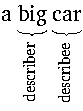
\includegraphics{A-Learners-Grammar-of-Classical-Standard-Arabic_files/figure-latex/unnamed-chunk-8-1.pdf}

We will reserve this terminology of \emph{describer} and \emph{describee} only for the noun and adjective in an descriptive noun-phrase. So we won't use this terminology for the sentence: \enquote{The car is big.}

Instead, here we will continue to use the existing terminology of \emph{subject} and \emph{information}. The definite noun \enquote{the car} is the subject of this sentence, and the adjective \enquote{big} is the information.

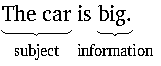
\includegraphics{A-Learners-Grammar-of-Classical-Standard-Arabic_files/figure-latex/unnamed-chunk-9-1.pdf}

\section{Adjectival nouns in English}\label{adjectival-nouns-in-english}

Consider the English word \enquote{antique}. It is what we will call a \emph{adjectival noun}.

It can be used just like an adjective to describe a noun as part of a noun-phrase. For example:

\enquote{The antique table is expensive.}

In the above sentence the adjective \enquote{antique} is a describer and is describing the noun \enquote{table}.

It can also be used as the information of a sentence, just like an adjective. For example:

\enquote{The table is antique.}

But what makes it different from an normal adjective is that it can also be used by itself as a noun. For example:

\enquote{The antique is expensive.}

Here \enquote{the antique} could refer to any entity that can be described by the quality of being old and valuable. The adjectival noun does not require any other noun in this sentence and can stand on its own as the subject of the sentence.

Adjectival nouns are rare in English. Instead, adjectives are usually used when we want to describe a noun.

\section{Adjectival nouns in Arabic and genderizability}\label{adjectival-nouns-in-arabic-and-genderizability}

Arabic does not have adjectives. It only has adjectival nouns.

The word \foreignlanguage{arabic}{صَغِير} \emph{ṣag͡hīr} is an example of an indefinite adjectival noun in Arabic. It describes the quality of being \enquote{small} or \enquote{little}. It can be used to denote any person, animal, or things that can be described as being small. Technically we could translate it as \enquote{a little one\textsubscript{m}} or \enquote{a small one\textsubscript{m}}.

Being a noun \foreignlanguage{arabic}{صَغِير} \emph{ṣag͡hīr}, like all other nouns in Arabic, will have a grammatical gender. Since it does not end with a feminine marker like \foreignlanguage{arabic}{ة}, we can state that
\foreignlanguage{arabic}{صَغِير} \emph{ṣag͡hīr} is a masculine noun.

Adjectival nouns, typically, are genderizable. This means that we can feminize
\foreignlanguage{arabic}{صَغِير} \emph{ṣag͡hīr} (masc.) to get the feminine noun.
We will feminize
\foreignlanguage{arabic}{صَغِير} \emph{ṣag͡hīr} (masc.) with the feminine marker \foreignlanguage{arabic}{ة} to get the feminine adjectival noun
\foreignlanguage{arabic}{صَغِيرَة} \emph{ṣag͡hīrah} (fem.) \enquote{a little one\textsubscript{f}}.

Generally, the dictionary will typically only supply the masculine adjectival noun.
And we are expected to know how to feminize it to get the feminine adjectival noun.

As opposed to adjectival nouns, common nouns are not genderizable. So, for example, if we know that the noun
\foreignlanguage{arabic}{غُلَام} \emph{g͡hulām} \enquote{a boy} exists, we cannot assume that we can feminize it, by using the feminine marker \foreignlanguage{arabic}{ة}, for example, getting: \(\times\) \foreignlanguage{arabic}{غُلَامَة} \emph{g͡hulāmah}. This would be a misguided attempt to obtain the meaning for \enquote{a girl} in Standard Arabic. Instead, we have to look up the Arabic word for \enquote{a girl} in the dictionary separately, and we find that it is \foreignlanguage{arabic}{جَارِيَة} \emph{jāriyah}.

Many times times, a masculine/feminine common noun pair will exist, that differ only by the feminine marker \foreignlanguage{arabic}{ة}. For example:

\begin{itemize}
\tightlist
\item
  \foreignlanguage{arabic}{ٱِبْن} \emph{ʾibn} \enquote{a son} and \foreignlanguage{arabic}{ٱِبْنَة} \emph{ʾibnah} \enquote{a daughter}.
\item
  \foreignlanguage{arabic}{مُعَلِّم} \emph{muɛallim} \enquote{a teacher\textsubscript{m}} and \foreignlanguage{arabic}{مُعَلِّمَة} \emph{muɛallimah} \enquote{a teacher\textsubscript{f}}
\end{itemize}

This does not indicate that the common noun is genderizable. Rather, when the common noun masc./fem. pair has a meaning that is derived from a verb or an adjective (like
\foreignlanguage{arabic}{مُعَلِّم}/\foreignlanguage{arabic}{مُعَلِّمَة}),
then the masculine/feminine pair are co-derived as separate non-genderizable words. We will discuss this in more detail in later chapters, if Allāh wills.

And when the common noun masc./fem. pair has a primitive (non-verbal and non-adjectival) meaning, (like
\foreignlanguage{arabic}{ٱِبْن}/\foreignlanguage{arabic}{ٱِبْنَة}),
then this is only a coincidence. We alluded to this in section~\ref{related-nouns-for-male-and-female-animate-beings}.

\subsection{Examples of Arabic adjectival nouns}\label{examples-of-arabic-adjectival-nouns}

Here are some examples of Arabic adjectival nouns that we will use in this chapter.

\begin{longtable}[]{@{}ll@{}}
\toprule\noalign{}
Arabic adjectival noun & Meaning \\
\midrule\noalign{}
\endhead
\bottomrule\noalign{}
\endlastfoot
\foreignlanguage{arabic}{کَبِير} \emph{kabīr} & a big one \\
\foreignlanguage{arabic}{صَغِير} \emph{ṣag͡hīr} & a small one \\
\foreignlanguage{arabic}{طَيِّب} \emph{ṭayyib} & a good one \\
\foreignlanguage{arabic}{قَدِيم} \emph{qadīm} & an old one \\
\foreignlanguage{arabic}{جَدِيد} \emph{jadīd} & a new one \\
\foreignlanguage{arabic}{طَوِيل} \emph{ṭawīl} & a long/tall one \\
\foreignlanguage{arabic}{وَاسِع} \emph{wāsiɛ} & a wide one \\
\foreignlanguage{arabic}{عَرَبِيّ} \emph{ɛarabiyy} & an Arab \\
\foreignlanguage{arabic}{مَشْهُور} \emph{mas͡h·hūr} & a famous one \\
\end{longtable}

\section{The describer and the describee in descriptive noun-phrases}\label{the-describer-and-the-describee-in-descriptive-noun-phrases}

Let's learn how descriptive noun-phrases are formed in Arabic.

We learned in section~\ref{terminology-the-describer-and-the-describee}
above that descriptive noun-phrases consist of a describer and a describee.

In English descriptive noun-phrases, like \enquote{the small house}, the adjective describer (\enquote{small}) comes before the describee (\enquote{house}). Also, only one definite article (\enquote{the}) is used before the entire noun-phrase.

Here is the equivalent Arabic descriptive noun-phrase:

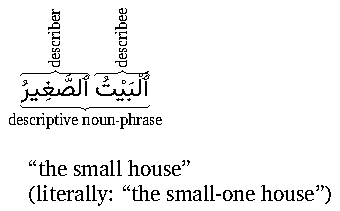
\includegraphics{A-Learners-Grammar-of-Classical-Standard-Arabic_files/figure-latex/unnamed-chunk-10-1.pdf}

Note the following:

\begin{itemize}
\tightlist
\item
  The adjectival noun describer \foreignlanguage{arabic}{ٱَلصَّغِير} \emph{ʾaṣṣag͡hīr} \enquote{the small one\textsubscript{m}} comes after the describee \foreignlanguage{arabic}{ٱَلْبَيْت} \emph{ʾalbayt} \enquote{the house}.
\item
  Both the adjectival noun describer \foreignlanguage{arabic}{ٱَلصَّغِير} \emph{ʾaṣṣag͡hīr} \enquote{the small one\textsubscript{m}} and the describee \foreignlanguage{arabic}{ٱَلْبَيْت} \emph{ʾalbayt} \enquote{the house} get the definite article \foreignlanguage{arabic}{ٱَلْ} \enquote{the}.
\item
  The adjectival noun describer \foreignlanguage{arabic}{ٱَلصَّغِير} \emph{ʾaṣṣag͡hīr} \enquote{the small one\textsubscript{m}} is genderized to match the describee \foreignlanguage{arabic}{ٱَلْبَيْت} \emph{ʾalbayt} \enquote{the house} in gender.
\item
  The adjectival noun describer \foreignlanguage{arabic}{ٱَلصَّغِير} \emph{ʾaṣṣag͡hīr} \enquote{the small one\textsubscript{m}} matches the describee \foreignlanguage{arabic}{ٱَلْبَيْت} \emph{ʾalbayt} \enquote{the house} in state. In this example, they were both in the u-state but we will see examples in the other states as well.
\item
  The word-for-word equivalence of the above descriptive noun-phrase is \enquote{the small-one house} but we will usually give the more natural translation: \enquote{the small house}
\end{itemize}

Let's try another example: let's try to translate the sentence: \enquote{The little girl took a new book from the good mother.}

Here is the sentence in Arabic:

\foreignlanguage{arabic}{أَخَذَتِ ٱلْجَارِيَةُ ٱلصَّغِيرَةُ کِتَابًا جَدِيدًا مِنْ ٱلْأُمِّ ٱلطَّيِّبَةِ.}\\
\emph{ʾak͡had͡hati -ljāriyatu -ṣṣag͡hīratu kitaban jadīdan mina -lʾummi -ṭṭayyibah.}\\
\enquote{The little girl took a new book from the good mother.}

This sentence has three descriptive noun-phrases. We will analyze each one individually:

\begin{enumerate}
\def\labelenumi{\roman{enumi}.}
\item
  \foreignlanguage{arabic}{ٱَلْجَارِيَةُ ٱلصَّغِيرَةُ}\\
  \emph{ʾaljāriyatu -ṣṣag͡hīratu}\\
  \enquote{the little girl}

  In this phrase the definite feminine noun \foreignlanguage{arabic}{ٱلْجَارِيَةُ} \emph{ʾaljāriyatu} is the doer of the verb \foreignlanguage{arabic}{أَخَذَ} \emph{ʾak͡had͡ha} \enquote{took}. Therefore it is in the u-state. It is also the describee in the descriptive noun-phrase. Its describer \foreignlanguage{arabic}{ٱَلصَّغِيرَةُ} \emph{ʾaṣṣag͡hīratu} follows the describee and is made to match the describee in state (u-state), gender (feminine), and definiteness (definite).
\item
  \foreignlanguage{arabic}{کِتَابًا جَدِيدًا}\\
  \emph{kitāban jadīdan}\\
  \enquote{a new book}

  In this phrase the indefinite masculine noun \foreignlanguage{arabic}{کِتَابًا} \emph{kitāban} is the doee of the verb \foreignlanguage{arabic}{أَخَذَ} \emph{ʾak͡had͡ha} \enquote{took}. Therefore it is in the a-state. It is also the describee in the descriptive noun-phrase. Its describer \foreignlanguage{arabic}{جَدِيدًا} \emph{jadīdan} follows the describee and is made to match the describee in state (a-state), gender (masculine), and definiteness (indefinite).
\item
  \foreignlanguage{arabic}{ٱَلْأُمِّ ٱلطَّيِّبَةِ}\\
  \emph{ʾalʾummi -ṭṭayyibati}\\
  \enquote{the good mother}

  In this phrase the definite feminine noun \foreignlanguage{arabic}{ٱلْأُمِّ} \emph{ʾalʾummi} is following the preposition \foreignlanguage{arabic}{مِنْ} \emph{min} \enquote{from}. Therefore it is in the i-state. It is also the describee in the descriptive noun-phrase. Its describer \foreignlanguage{arabic}{ٱَلطَيِّبَةِ} \emph{ʾaṭṭayyibati} follows the describee and is made to match the describee in state (i-state), gender (feminine), and definiteness (definite).

  Note carefully that the describer matches the describee in gender, not necessarily in having the same \foreignlanguage{arabic}{ة} ending. The feminine adjectival noun describer \foreignlanguage{arabic}{ٱَلطَيِّبَة} \emph{ʾaṭṭayyibah} is still formed using the feminine marker \foreignlanguage{arabic}{ة}, despite the feminine describee \foreignlanguage{arabic}{ٱَلْأُمّ} not having the \foreignlanguage{arabic}{ة} feminine marker.
\end{enumerate}

Sometimes, a common noun of one gender is used to refer to persons of either gender. For example:

\begin{itemize}
\tightlist
\item
  the noun \foreignlanguage{arabic}{شَخْص} \emph{s͡hak͡hṣ} is itself a masculine noun but it may be used to refer to both male and female persons.
\end{itemize}

If such a noun is a describee, then we will prefer to match the describer to the grammatical gender of the noun, not the physical gender of the person it is referring to. For example:

\foreignlanguage{arabic}{ٱَلْجَارِيَةُ شَخْصٌ طَيِّبٌ.}\\
\emph{ʾaljāriyatu s͡hak͡hṣun ṭayyib.}\\
\enquote{The girl is a good person.}

See how we preferred to use the masculine adjectival noun \foreignlanguage{arabic}{طَيِّب} \emph{ṭayyib} instead of using the feminine \foreignlanguage{arabic}{طَيِّبَة} \emph{ṭayyibah}.

\section{Adjectival nouns as the information of a sentence}\label{adjectival-nouns-as-the-information-of-a-sentence}

\subsection{Indefinite adjectival noun}\label{indefinite-adjectival-noun}

Let's see how to use Arabic adjectival nouns as the information of a sentence.

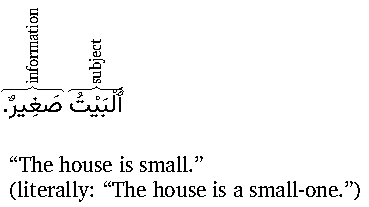
\includegraphics{A-Learners-Grammar-of-Classical-Standard-Arabic_files/figure-latex/unnamed-chunk-11-1.pdf}

In the above sentence, the indefinite adjectival noun
\foreignlanguage{arabic}{صَغِير} \emph{ṣag͡hīr} \enquote{a small one}
is used as the information of a sentence. Its indefiniteness and u-state is indicated by the nūnated \emph{u}-mark \foreignlanguage{arabic}{◌ٌ} on its end.

When an adjectival noun is the information of a sentence, then it shall be genderized to match the gender of the subject noun. The subject noun in this case (\foreignlanguage{arabic}{ٱَلْبَيْت}) is masculine. Therefore, the masculine adjectival noun (\foreignlanguage{arabic}{صَغِير}) is chosen.

Technically, the translation of this sentence is \enquote{The house is a small one.}
However, because Arabic has only adjectival nouns and not adjectives, it is how we can express the English sentence \enquote{The house is small.} Therefore we can also translate it into English as such.

Now let's try a sentence with a feminine subject:

\foreignlanguage{arabic}{ٱَلْجَارِيَةُ صَغِيرَة.}\\
\emph{ʾaljāriyatu ṣag͡hīrah}\\
\enquote{The girl is a little one\textsubscript{f}.} = \enquote{The girl is little.}

In the above example the subject (\foreignlanguage{arabic}{ٱَلْجَارِيَة} \enquote{the girl}) was feminine. Therefore, we feminized the masculine adjectival noun \foreignlanguage{arabic}{صَغِير} \emph{ṣag͡hīr} with the feminine marker \foreignlanguage{arabic}{ة} to get the feminine adjectival noun
\foreignlanguage{arabic}{صَغِيرَة} \emph{ṣag͡hīrah} \enquote{a little one\textsubscript{f}}
and used the feminine adjectival noun in the sentence.

\subsection{Definite adjectival noun}\label{definite-adjectival-noun}

Let's see if a definite adjectival noun can be used in the information. For example, we would like to say \enquote{The old tree is the big one.}

The subject of the sentence is \foreignlanguage{arabic}{ٱَلشَّجَرَةُ ٱلْقَدِيمَةُ} \emph{ʾas͡hs͡hajaratu -lqadīmuiatu} \enquote{the old tree}.
And the information is \foreignlanguage{arabic}{ٱلْکَبِيرَةُ} \emph{ʾalkabīratu} \enquote{the big one}. When we put the two together we get:

\foreignlanguage{arabic}{ٱَلشَّجَرَةُ ٱلْقَدِيمَةُ ٱلْکَبِيرَةُ}\\
\emph{ʾas͡hs͡hajaratu -lqadīmatu -lkabīratu}

The problem is that the above could also be interpreted as one phrase \enquote{the big old tree}, and not as the complete sentence \enquote{The old tree is the big one.} This is the same problem that we highlighted in section~\ref{chap-smp-sent-sec-def-info}.

The solution, too, is the same. We insert a detached pronoun, that matches the gender of the subject, between the subject and the information. So in order to get our intended meaning, we will say:

\foreignlanguage{arabic}{ٱَلشَّجَرَةُ ٱلْقَدِيمَةُ هِيَ ٱلْکَبِيرَةُ.}\\
\emph{ʾas͡hs͡hajaratu -lqadīmatu hiya -lkabīratu.}\\
\enquote{The old tree is the big one.}

\section{Adjectival nouns used without a described noun}\label{adjectival-nouns-used-without-a-described-noun}

We have mentioned that adjectival nouns are just like other nouns that we have learned so far, in that they have gender, state, and definiteness. Can we then use
an adjectival noun by itself and not when it is describing another noun?

The answer is yes, we can. So for example, you can say:

\foreignlanguage{arabic}{شَرِبَ ٱلصَّغِيرُ حَلِيبًا.}\\
\emph{s͡hariba -ṣṣag͡hīru ḥalībā.}\\
\enquote{The little one drank some milk.}

The above is a correct sentence. But, by itself, it is not very clear. What do we mean by \enquote{the little one}? Is it a little boy, or a little cat, or something else? So, context would be needed to know what exactly is being denoted by the adjectival noun when it is used by itself independently.

Here is the same sentence again, but this time with some clarifying context.

\foreignlanguage{arabic}{حَمَلَتِ ٱلْأُمُّ ٱلصَّغِيرَ. وَشَرِبَ ٱلصَّغِيرُ حَلِيبًا.}\\
\emph{ḥamalati -lʾummu -ṣṣag͡hīra. was͡hariba -ṣṣag͡hīru ḥalībā.}\\
\enquote{The mother carried the little one. And the little one drank some milk.}

So now we can tell that what is meant by \foreignlanguage{arabic}{ٱلصَّغِير} \emph{ʾaṣṣag͡hīr} \enquote{the little one} here is \enquote{the baby}.

\section{Adjectival nouns re-used as common nouns}\label{adjectival-nouns-re-used-as-common-nouns}

Sometimes, an adjectival noun, through much usage, acquires the meaning of a common noun. It then gets listed with this meaning in the dictionary. We actually just saw an example above. The adjectival noun
\foreignlanguage{arabic}{صَغِير} \emph{ṣag͡hīr} \enquote{a little one} is commonly used to mean \enquote{a baby}. Of course, context would be needed to know whether, in a particular sentence, it has its common noun meaning: \enquote{a baby}, or its general adjectival noun meaning: \enquote{a little one}.

The opposite of
\foreignlanguage{arabic}{صَغِير} \emph{ṣag͡hīr} \enquote{a little one}
is \foreignlanguage{arabic}{کَبِير} \emph{kabīr} \enquote{a big one}. It too has acquired the common noun meaning of \enquote{an elder person}. Here is an example of its usage:

\foreignlanguage{arabic}{قَدِمَ ٱلْکَبِيرُ وَوَعَظَ ٱلْغُلَامَ.}\\
\emph{qadima -lkabīru wawaɛaḍ͡ha -lg͡hulāma.}\\
\enquote{The elder arrived and admonished the boy.}

When an adjectival noun gets re-used as a common noun, it loses its genderizability.
For example, the feminine adjectival noun \foreignlanguage{arabic}{حَسَنَة} \emph{ḥasanah} (fem.) \enquote{a good one} is re-used as a common noun meaning \enquote{a good deed}. So we can use it in a sentence:

\foreignlanguage{arabic}{ٱلصِّيَامُ حَسَنَةٌ.}\\
\emph{ʾaṣṣiyāmu ḥasanah.}\\
\enquote{Fasting is a good deed.}

The subject in this sentence is the masculine noun \foreignlanguage{arabic}{ٱَلصِّيَام} \emph{ʾaṣṣiyām} \enquote{fasting}.
And the information is the feminine noun \foreignlanguage{arabic}{حَسَنَة} \emph{ḥasanah} \enquote{a good deed}.
Note that the information does not match the subject in gender. This is because it lost its genderizability since it is no longer acting as an adjectival noun \enquote{a good one\textsubscript{f}}, but rather as the common noun \enquote{a good deed}.

What if we have the sentence:

\foreignlanguage{arabic}{ٱَلصَّدَقَةُ حَسَنَةٌ.}\\
\emph{ʾaṣṣadaqatu ḥasanah.}

The feminine gender of the subject
\foreignlanguage{arabic}{ٱَلصَّدَقَة.}
\emph{ʾaṣṣadaqah} \enquote{charity} now matches the gender of the information
\foreignlanguage{arabic}{حَسَنَة} \emph{ḥasanah}.
So now, technically, the information could be the adjectival noun, meaning \enquote{a good one\textsubscript{f}}. So the sentence could mean:

\enquote{Charity is good.}

Or the information could be the common noun, meaning \enquote{a good deed}. Then the sentence would mean:

\enquote{Charity is a good deed.}

Context would be needed to tell us which meaning is intended.

\section{Common-nouns used as describers in a noun-phrase}\label{common-nouns-used-as-describers-in-a-noun-phrase}

Usually, adjectival nouns are used as the describer in an descriptive noun-phrase. However, we also often find a common noun used as a describer. For example,

\foreignlanguage{arabic}{هُوَ رَجُلٌ مُعَلِّمٌ.}\\
\emph{huwa rajulun muɛallim.}\\
\enquote{He is a teacher\textsubscript{m} man.}\\
= \enquote{He is a man who is a teacher\textsubscript{m}.}

\section{Multiple adjectival nouns describing the same noun}\label{multiple-adjectival-nouns-describing-the-same-noun}

In English we can have a noun described by multiple adjectives separated by commas and the word \enquote{and}. For example, \enquote{The building is big, tall, and wide.} In Arabic we will separate the multiple adjectival nouns with \foreignlanguage{arabic}{وَ} \emph{wa-} \enquote{and}:

\foreignlanguage{arabic}{ٱَلْبِنَاءُ کَبِيرٌ وَطَوِيلٌ وَوَاسِعٌ.}\\
\emph{ʾalbināʾu kabīrun waṭawīlun wawāsiʾun}\\
\enquote{The building is big and tall and wide.}

In an English descriptive noun-phrase, multiple describers may describe the same describee, without being separated by the word \enquote{and}. For example, \enquote{The man is a famous Arab writer.} In Arabic, we can do the same, except the describees will be in the reverse order:

\foreignlanguage{arabic}{ٱَلرَّجُلُ کَاتِبٌ عَرَبِيٌّ مَشْهُورٌ.}\\
\emph{ʾarrujulu kātibun ɛarabiyyun mas͡h·hūr.}\\
\enquote{The man is a famous Arab writer.}

\section{A prepositional phrase separating the describer from the describee}\label{a-prepositional-phrase-separating-the-describer-from-the-describee}

Consider the phrase:

\foreignlanguage{arabic}{کِتَابٌ مِنَ ٱلْمَکْتَبَةِ}\\
\emph{kitābun mina -lmaktabati}\\
\enquote{a book from the library}

If we want to add a adjectival noun as to describe \enquote{the book}, we may add it either before or after the prepositional phrase describer. Here are both examples as complete sentences:

\foreignlanguage{arabic}{قَرَأَ کِتَابًا صَغِيرًا مِنَ ٱلْمَکْتَبَةِ.}\\
\emph{qaraʾa kitāban ṣag͡hīran mina -lmaktabati.}\\
AND\\
\foreignlanguage{arabic}{قَرَأَ کِتَابًا مِنَ ٱلْمَکْتَبَةِ صَغِيرًا.}\\
\emph{qaraʾa kitāban mina -lmaktabati ṣag͡hīran.}\\
\enquote{a small book from the library}

The first option is usually chosen as a matter of preference but the second option is legitimate too.

\chapter{Semi-flexible nouns}\label{semi-flexible-nouns}

\section{Introduction}\label{introduction-6}

Nouns are of two main categories of nouns, with regard to their endings in the different noun states:

\begin{enumerate}
\def\labelenumi{\arabic{enumi}.}
\tightlist
\item
  Rigid nouns.
\item
  Flexible nouns. These are further sub-divided into:

  \begin{enumerate}
  \def\labelenumii{\roman{enumii}.}
  \tightlist
  \item
    Fully-flexible nouns.
  \item
    Semi-flexible nouns.
  \end{enumerate}
\end{enumerate}

So far we have been mostly studying fully-flexible nouns. In this chapter we will learn about semi-flexible nouns.

Here is an example of the kind of nouns we have learned so far:

\begin{longtable}[]{@{}lll@{}}
\toprule\noalign{}
State & Indefinite & Definite \\
\midrule\noalign{}
\endhead
\bottomrule\noalign{}
\endlastfoot
u-state & \foreignlanguage{arabic}{رَجُلٌ} & \foreignlanguage{arabic}{ٱَلرَّجُلُ} \\
a-state & \foreignlanguage{arabic}{رَجُلًا} & \foreignlanguage{arabic}{ٱَلرَّجُلَ} \\
i-state & \foreignlanguage{arabic}{رَجُلٍ} & \foreignlanguage{arabic}{ٱَلرَّجُلِ} \\
\end{longtable}

As you can see, the noun is nūnated when it is indefinite, and also, the vowel mark on the last letter changes for each state that the noun is in. These kinds of nouns are called \emph{fully-flexible} nouns. They are by far the most common type of noun.

There are some nouns, however, that are \emph{semi-flexible}.
Here is an example of a semi-flexible noun, \foreignlanguage{arabic}{صَحْرَاء} \emph{ṣaḥrāʾ} \enquote{a desert}:

\begin{longtable}[]{@{}lll@{}}
\toprule\noalign{}
State & Indefinite & Definite \\
\midrule\noalign{}
\endhead
\bottomrule\noalign{}
\endlastfoot
u-state & \foreignlanguage{arabic}{صَحْرَاءُ} & \foreignlanguage{arabic}{ٱَلصَّحْرَاءُ} \\
a-state & \foreignlanguage{arabic}{صَحْرَاءَ} & \foreignlanguage{arabic}{ٱَلصَّحْرَاءَ} \\
i-state & \foreignlanguage{arabic}{صَحْرَاءَ} & \foreignlanguage{arabic}{ٱَلصَّحْرَاءِ} \\
\end{longtable}

As you can see, when \foreignlanguage{arabic}{صَحْرَاء} \emph{ṣaḥrāʾ} is indefinite, it is not nūnated. Also, when it is indefinite and in the i-state, the vowel mark on its final letter is not \foreignlanguage{arabic}{◌ِ}, as you might expect but \foreignlanguage{arabic}{◌َ} . And so the noun looks identical in the a-state and i-state when it is indefinite.

When it is definite, however, it looks just like fully-flexible nouns.

So there are two differences between fully-flexible and semi-flexible nouns:

\begin{enumerate}
\def\labelenumi{\arabic{enumi}.}
\tightlist
\item
  When indefinite, a semi-flexible noun is not nūnated.
\item
  When indefinite and in the i-state, a semi-flexible noun's final letter does not have an \emph{i}-mark. Instead it shall have an \emph{a}-mark, just like when it is in the a-state.
\end{enumerate}

The other category of nouns are \emph{rigid} nouns. Rigid nouns don't change their endings due to their state. They are much fewer in number compared to flexible nouns. Pronouns are an example of rigid nouns.

\section{Feminine markers}\label{feminine-markers}

Before we discuss semi-flexible nouns in more detail, we will discuss feminine markers. We already know of one feminine marker: the \foreignlanguage{arabic}{ة}. When a singular noun ends with \foreignlanguage{arabic}{ة}, then that is an indication, with very few exceptions, that it is a feminine noun. Examples are:

\begin{longtable}[]{@{}
  >{\raggedright\arraybackslash}p{(\columnwidth - 4\tabcolsep) * \real{0.1111}}
  >{\raggedright\arraybackslash}p{(\columnwidth - 4\tabcolsep) * \real{0.4444}}
  >{\raggedright\arraybackslash}p{(\columnwidth - 4\tabcolsep) * \real{0.4444}}@{}}
\toprule\noalign{}
\begin{minipage}[b]{\linewidth}\raggedright
Root
\end{minipage} & \begin{minipage}[b]{\linewidth}\raggedright
Feminine noun
\end{minipage} & \begin{minipage}[b]{\linewidth}\raggedright
Masculine noun from same root (if any)
\end{minipage} \\
\midrule\noalign{}
\endhead
\bottomrule\noalign{}
\endlastfoot
\foreignlanguage{arabic}{«جري»} & \foreignlanguage{arabic}{جَارِيَة} \enquote{a girl\textsubscript{f}} & -- \\
\foreignlanguage{arabic}{«علم»} & \foreignlanguage{arabic}{عَالِمَة} \enquote{a scholar\textsubscript{f}} & \foreignlanguage{arabic}{عَالِم} \enquote{a scholar\textsubscript{m}} \\
\foreignlanguage{arabic}{«کلب»} & \foreignlanguage{arabic}{کَلْبَة} \enquote{a dog\textsubscript{f}} & \foreignlanguage{arabic}{کَلْب} \enquote{a dog\textsubscript{m}} \\
\foreignlanguage{arabic}{«شجر»} & \foreignlanguage{arabic}{شَجَرَة} \enquote{a tree} & -- \\
\foreignlanguage{arabic}{«صغر»} & \foreignlanguage{arabic}{صَغِيرَة} \emph{adj.} \enquote{small\textsubscript{f}} & \foreignlanguage{arabic}{صَغِير} \emph{adj.} \enquote{small\textsubscript{m}} \\
\end{longtable}

As you can see, the feminine marker \foreignlanguage{arabic}{ة} is never part of the noun's root. It is thus considered \emph{extrinsic} to the root. Also, sometimes, but not always, the feminine noun is formed by adding the feminine marker \foreignlanguage{arabic}{ة} to the end of a masculine noun.

It is also important to note that \foreignlanguage{arabic}{ة} is only a feminine marker for singular nouns. When we learn plurals, if Allāh wills, we will see that \foreignlanguage{arabic}{ة} is used frequently with masculine plurals.

Now we will learn of two more feminine markers: \foreignlanguage{arabic}{اء} and \foreignlanguage{arabic}{ىٰ}.

Here are some examples of nouns that end with these two feminine markers:

\begin{longtable}[]{@{}
  >{\raggedright\arraybackslash}p{(\columnwidth - 4\tabcolsep) * \real{0.1111}}
  >{\raggedright\arraybackslash}p{(\columnwidth - 4\tabcolsep) * \real{0.4444}}
  >{\raggedright\arraybackslash}p{(\columnwidth - 4\tabcolsep) * \real{0.4444}}@{}}
\toprule\noalign{}
\begin{minipage}[b]{\linewidth}\raggedright
Root
\end{minipage} & \begin{minipage}[b]{\linewidth}\raggedright
Feminine noun
\end{minipage} & \begin{minipage}[b]{\linewidth}\raggedright
Masculine noun (if any)
\end{minipage} \\
\midrule\noalign{}
\endhead
\bottomrule\noalign{}
\endlastfoot
\foreignlanguage{arabic}{«صحر»} & \foreignlanguage{arabic}{صَحْرَاء} \enquote{a desert} & -- \\
\foreignlanguage{arabic}{«حمر»} & \foreignlanguage{arabic}{حَمْرَاء} \emph{adj.} \enquote{red\textsubscript{f}} & \foreignlanguage{arabic}{أَحْمَر} \emph{adj.} \enquote{red\textsubscript{m}} \\
\foreignlanguage{arabic}{«ذکر»} & \foreignlanguage{arabic}{ذِکْرَىٰ} \enquote{a remembrance} & -- \\
\foreignlanguage{arabic}{«غضب»} & \foreignlanguage{arabic}{غَضْبَىٰ} \emph{adj.} \enquote{very angry\textsubscript{f}} & \foreignlanguage{arabic}{غَضْبَان} \emph{adj.} \enquote{very angry\textsubscript{m}} \\
\end{longtable}

When extrinsic to the word's root, \foreignlanguage{arabic}{اء} and \foreignlanguage{arabic}{ىٰ} are feminine markers, just like \foreignlanguage{arabic}{ة}. However, one important difference from \foreignlanguage{arabic}{ة} is that sometimes
\foreignlanguage{arabic}{اء} and \foreignlanguage{arabic}{ىٰ} may not be extrinsic to the word's root. In this case, they will not be feminine markers, and the noun will regularly be a masculine noun. Examples:

\begin{longtable}[]{@{}
  >{\raggedright\arraybackslash}p{(\columnwidth - 4\tabcolsep) * \real{0.1579}}
  >{\raggedright\arraybackslash}p{(\columnwidth - 4\tabcolsep) * \real{0.5789}}
  >{\raggedright\arraybackslash}p{(\columnwidth - 4\tabcolsep) * \real{0.2632}}@{}}
\toprule\noalign{}
\begin{minipage}[b]{\linewidth}\raggedright
Root
\end{minipage} & \begin{minipage}[b]{\linewidth}\raggedright
Noun
\end{minipage} & \begin{minipage}[b]{\linewidth}\raggedright
Pattern using paradigm \foreignlanguage{arabic}{«فعل»}
\end{minipage} \\
\midrule\noalign{}
\endhead
\bottomrule\noalign{}
\endlastfoot
\foreignlanguage{arabic}{«هدي»} & \foreignlanguage{arabic}{ٱلْهُدَىٰ} (masc.) \enquote{the guidance} & \foreignlanguage{arabic}{ٱَلْفُعَل} \\
\foreignlanguage{arabic}{«خبء»} & \foreignlanguage{arabic}{خِبَاء} (masc.) \enquote{a tent} & \foreignlanguage{arabic}{فِعَال} \\
\end{longtable}

These cases will become more clear, if Allāh wills, when we study weak roots (roots that contain a weak letter like \foreignlanguage{arabic}{ء، و، ي}).

Otherwise,
when extrinsic to the word's root, \foreignlanguage{arabic}{اء}, and \foreignlanguage{arabic}{ىٰ} are consistently feminine markers, just like \foreignlanguage{arabic}{ة}.

Also, just like \foreignlanguage{arabic}{ة}, \foreignlanguage{arabic}{اء} and \foreignlanguage{arabic}{ىٰ} are only feminine markers for singular nouns. We will see, if Allāh wills, that they are used frequently with masculine plurals.

By the way, another difference from \foreignlanguage{arabic}{ة} is that when
\foreignlanguage{arabic}{اء} and \foreignlanguage{arabic}{ىٰ} are feminine markers, and a masculine counterpart exists, then the feminine noun is not formed by simply adding the feminine marker to the end of the masculine noun. The masculine and feminine nouns are different internally as well. For example, the feminine noun
\foreignlanguage{arabic}{حَمْرَاء} \emph{adj.} \enquote{red\textsubscript{f}}
is not formed simply by adding the feminine marker \foreignlanguage{arabic}{اء} to the end of the masculine noun
\foreignlanguage{arabic}{أَحْمَر} \emph{adj.} \enquote{red\textsubscript{m}}.

We will discuss this in more detail below.

\section{Categories of semi-flexible nouns}\label{categories-of-semi-flexible-nouns}

We now return to our discussion of semi-flexible nouns. Semi-flexible nouns, in terms of their formation, fall under different categories. We will discuss them below.

When discussing semi-flexible nouns in isolation we will add the numeral~2 as a superscript to their ending, thus:
\textsuperscript{2}\foreignlanguage{arabic}{صَحْرَاء} \emph{ṣaḥrāʾ}\textsuperscript{2}. This is to indicate their semi-flexibility.

\subsection{\texorpdfstring{Nouns that end with an extrinsic \foreignlanguage{arabic}{اء}}{Nouns that end with an extrinsic اء}}\label{nouns-that-end-with-an-extrinsic-ux627ux621}

If a noun ends with an \foreignlanguage{arabic}{اء}, which is extrinsic to the word's root, then it shall be a semi-flexible noun.

We have already seen an example of such a noun above: \textsuperscript{2}\foreignlanguage{arabic}{صَحْرَاء} \emph{ṣaḥrāʾ}\textsuperscript{2} \enquote{a desert}. The root of this noun is \foreignlanguage{arabic}{«صحر»}. You can see that the ending \foreignlanguage{arabic}{اء} is not part of the root. Therefore it is a semi-flexible noun.

Furthermore, we have also learned that this \foreignlanguage{arabic}{اء}, which is extrinsic to the word's root, is a feminine marker for singular nouns, just like \foreignlanguage{arabic}{ة}, except that \foreignlanguage{arabic}{ة} does not generally make a noun semi-flexible.

Here is an example sentence with this noun:

\foreignlanguage{arabic}{ذَهَبَ ٱلرَّجُلُ إِلَىٰ صَحْرَاءَ وَاسِعَةٍ.}\\
\emph{d͡hahaba -rrajulu ʾilā ṣaḥrāʾa wāsiɛah.}\\
\enquote{The man went to a wide desert.}

Note that the vowel mark on the final letter of \foreignlanguage{arabic}{صَحْرَاءَ} \emph{ṣaḥrāʾa} is \foreignlanguage{arabic}{◌َ}, not \foreignlanguage{arabic}{◌ٍ}, even though it is indefinite and in the i-state (because it is preceded by the preposition \foreignlanguage{arabic}{إِلَىٰ} \emph{ʾilā} \enquote{to}). This is because it is a semi-flexible noun.

\textsuperscript{2}\foreignlanguage{arabic}{صَحْرَاء} \emph{ṣaḥrāʾ}\textsuperscript{2} in this sentence
is also a describee, whose describer is \foreignlanguage{arabic}{وَاسِعَةٍ} \emph{wāsiɛatin} \enquote{wide}. The final vowel mark \foreignlanguage{arabic}{◌َ} on the describee \foreignlanguage{arabic}{صَحْرَاءَ} \emph{ṣaḥrāʾa} has no effect on the final vowel mark on the describer \foreignlanguage{arabic}{وَاسِعَةٍ} \emph{wāsiɛatin} \enquote{wide}. All that matters in this regard is the state of the describee.

Note, also, that the describer \foreignlanguage{arabic}{وَاسِعَة} is feminine to match the gender of the describee
\textsuperscript{2}\foreignlanguage{arabic}{صَحْرَاء} \emph{ṣaḥrāʾ}\textsuperscript{2}.

Note, as well, that the describer \foreignlanguage{arabic}{وَاسِعَةٍ} is nūnated as it is indefinite and fully-flexible. The inability of its describee
\textsuperscript{2}\foreignlanguage{arabic}{صَحْرَاء} \emph{ṣaḥrāʾ}\textsuperscript{2}
to be nūnated (because of its semi-flexibility) does not affect the describer.

Also, beware, as we've already mentioned, that there are some words where the \foreignlanguage{arabic}{اء} ending may be part of the word's root, for example
\foreignlanguage{arabic}{خِبَاء} \emph{k͡hibāʾ} \enquote{a tent} from the root \foreignlanguage{arabic}{«خبء»} on the pattern \foreignlanguage{arabic}{خِبَاء}. Such words will be fully flexible.
Also, for the same reason, \foreignlanguage{arabic}{اء} in this word is not a feminine marker, and the word is masculine.

\subsection{\texorpdfstring{Nouns that end with an extrinsic \foreignlanguage{arabic}{ىٰ}}{Nouns that end with an extrinsic ىٰ}}\label{nouns-that-end-with-an-extrinsic-ux649}

If a noun ends with an \foreignlanguage{arabic}{ىٰ} which is extrinsic to the word's root, then it shall be a semi-flexible noun.

We've already seen an example of such a word: \textsuperscript{2}\foreignlanguage{arabic}{ذِکْرَىٰ} \emph{d͡hikrā}\textsuperscript{2} \enquote{a remembrance}. The root of this word is \foreignlanguage{arabic}{«ذکر»} and it is on the pattern \foreignlanguage{arabic}{فِعْلَىٰ}.

We've also learned that, similar to \foreignlanguage{arabic}{اء}, this \foreignlanguage{arabic}{ىٰ}, which is extrinsic to the word's root, is a feminine marker for singular nouns.

Since \textsuperscript{2}\foreignlanguage{arabic}{ذِکْرَىٰ} \emph{d͡hikrā}\textsuperscript{2} already ends with the vowel-mark \foreignlanguage{arabic}{◌ٰ}, the last letter won't have any additional vowel markers and therefore the word will appear the same in all states:

\begin{longtable}[]{@{}lll@{}}
\toprule\noalign{}
State & Indefinite & Definite \\
\midrule\noalign{}
\endhead
\bottomrule\noalign{}
\endlastfoot
u-state & \foreignlanguage{arabic}{ذِکْرَىٰ} & \foreignlanguage{arabic}{ٱَلذِّکْرَىٰ} \\
a-state & \foreignlanguage{arabic}{ذِکْرَىٰ} & \foreignlanguage{arabic}{ٱَلذِّکْرَىٰ} \\
i-state & \foreignlanguage{arabic}{ذِکْرَىٰ} & \foreignlanguage{arabic}{ٱَلذِّکْرَىٰ} \\
\end{longtable}

Therefore, the state of such nouns cannot be determined by the vowel mark on their final letter, and has to be deduced otherwise by their function in the sentence.
Nevertheless, these nouns are still included in the category of semi-flexible nouns, and not rigid nouns. This is because rigid nouns are closed set consisting only of pronouns and other similar words.

Here is an example of this word in a sentence:

\foreignlanguage{arabic}{ٱَلْکِتَابُ ذِکْرَىٰ جَمِيلةٌ.}\\
\emph{ʾalkitābu d͡hikrā jamīlah.}\\
\enquote{The book is a beautiful remembrance.}

Note, again how the describer \foreignlanguage{arabic}{جَمِيلَة} \emph{jamīlah} is feminine and in the u-state, in order to match the gender and state of the describee \textsuperscript{2}\foreignlanguage{arabic}{ذِکْرَىٰ} \emph{d͡hikrā}\textsuperscript{2}.

Beware also that, just like in the case of \foreignlanguage{arabic}{اء}, there are some words where \foreignlanguage{arabic}{ىٰ} may be part of the word's root, e.g.~\foreignlanguage{arabic}{ٱَلْهُدَىٰ} \emph{ʾalhudā} \enquote{the guidance} whose root is \foreignlanguage{arabic}{«هدي»}. Because here the \foreignlanguage{arabic}{ىٰ} in \foreignlanguage{arabic}{ٱلْهُدَىٰ} is part of the word's root, therefore it shall not be a semi-flexible noun. So, when it is indefinite, it will be nūnated: \foreignlanguage{arabic}{هُدًى} \emph{hudan} \enquote{a guidance}. Also, for the same reason, \foreignlanguage{arabic}{ىٰ} in this word is not a feminine marker, and the word is masculine.

\subsection{\texorpdfstring{Nouns on the pattern \foreignlanguage{arabic}{أَفْعَل}}{Nouns on the pattern أَفْعَل}}\label{nouns-on-the-pattern-ux623ux641ux639ux644}

If a noun is on the pattern \foreignlanguage{arabic}{أَفْعَل} \emph{ʾafɛal} then it shall be a semi-flexible noun. By the way, there is no feminine marker on such words, so they will be masculine by default.

Most colors and many physical characteristics fall into this pattern. Colors and physical characteristics are adjectival nouns. The masculine noun for such adjectival-nouns is on the pattern \foreignlanguage{arabic}{أَفْعَل} \emph{ʾafɛal}. And the feminine adjectival noun is on the pattern \foreignlanguage{arabic}{فَعْلَاء} \emph{faɛlāʾ} (which is itself a semi-flexible noun pattern because of the extrinsic \foreignlanguage{arabic}{اء} ending). Here are some examples of such adjectival nouns:

\begin{longtable}[]{@{}
  >{\raggedright\arraybackslash}p{(\columnwidth - 6\tabcolsep) * \real{0.1136}}
  >{\raggedright\arraybackslash}p{(\columnwidth - 6\tabcolsep) * \real{0.2727}}
  >{\raggedright\arraybackslash}p{(\columnwidth - 6\tabcolsep) * \real{0.3182}}
  >{\raggedright\arraybackslash}p{(\columnwidth - 6\tabcolsep) * \real{0.2955}}@{}}
\toprule\noalign{}
\begin{minipage}[b]{\linewidth}\raggedright
Root
\end{minipage} & \begin{minipage}[b]{\linewidth}\raggedright
Masc. Noun
\end{minipage} & \begin{minipage}[b]{\linewidth}\raggedright
Fem. noun
\end{minipage} & \begin{minipage}[b]{\linewidth}\raggedright
Meaning
\end{minipage} \\
\midrule\noalign{}
\endhead
\bottomrule\noalign{}
\endlastfoot
\foreignlanguage{arabic}{«حمر»} & \textsuperscript{2}\foreignlanguage{arabic}{أَحْمَر} & \textsuperscript{2}\foreignlanguage{arabic}{حَمْرَاء} & red \\
\foreignlanguage{arabic}{«سود»} & \textsuperscript{2}\foreignlanguage{arabic}{أَسْوَد} & \textsuperscript{2}\foreignlanguage{arabic}{سَوْدَاء} & black \\
\foreignlanguage{arabic}{«بيض»} & \textsuperscript{2}\foreignlanguage{arabic}{أَبْيَض} & \textsuperscript{2}\foreignlanguage{arabic}{بَيْضَاء} & white \\
\foreignlanguage{arabic}{«عرج»} & \textsuperscript{2}\foreignlanguage{arabic}{أَعْرَج} & \textsuperscript{2}\foreignlanguage{arabic}{عَرْجَاء} & lame \\
\foreignlanguage{arabic}{«حور»} & \textsuperscript{2}\foreignlanguage{arabic}{أَحْوَر} & \textsuperscript{2}\foreignlanguage{arabic}{حَوْرَاء} & beautiful eyed \\
\foreignlanguage{arabic}{«بکم»} & \textsuperscript{2}\foreignlanguage{arabic}{أَبْکَم} & \textsuperscript{2}\foreignlanguage{arabic}{بَکْمَاء} & mute \\
\end{longtable}

Example:

\foreignlanguage{arabic}{لَبِسَ ٱلرَّجُلُ قَمِيصًا أَبْيَضُ.}\\
\emph{labisa -rrajulu qamīṣan ʾabyaḍ.}\\
\enquote{The man wore a white shirt.}

\subsection{\texorpdfstring{Adjectival nouns that end with an extrinsic \foreignlanguage{arabic}{ان}}{Adjectival nouns that end with an extrinsic ان}}\label{adjectival-noun-an-diptote}

The letters \foreignlanguage{arabic}{ان} may be an extrinsic ending for nouns. This ending is not a feminine marker so the noun would typically be masculine. This ending may cause the noun to be semi-flexible.

This category is more complicated than the previous ones. The following conditions must be satisfied for a word that ends with \foreignlanguage{arabic}{ان} to be a semi-flexible noun:

\begin{enumerate}
\def\labelenumi{\arabic{enumi}.}
\tightlist
\item
  The noun must be a adjectival-noun on the pattern \foreignlanguage{arabic}{فَعْلَان}. So the common noun \foreignlanguage{arabic}{ثُعْبَان} \emph{t͡huɛbān} \enquote{a serpent} of the root \foreignlanguage{arabic}{«ثعي»} is a common noun and therefore, not a semi-flexible noun.
\item
  The \foreignlanguage{arabic}{ان} must be extrinsic to the word's root. So \foreignlanguage{arabic}{جَبَان} \emph{jabānun} \enquote{cowardly}, an adjectival noun of the root \foreignlanguage{arabic}{«جبن»}, is not a semi-flexible noun.
\item
  The feminine of the adjectival noun shall not be formed by adding \foreignlanguage{arabic}{ة} to the masculine noun. So \foreignlanguage{arabic}{نَدْمَان} \emph{nadmān} \enquote{regretful}, an adjectival-noun from the root \foreignlanguage{arabic}{«ندم»}, is not a semi-flexible noun, because its feminine is \foreignlanguage{arabic}{نَدْمَانَة} \emph{nadmānah}.
\end{enumerate}

It is rare that this last condition fails. Most adjectival nouns that end with an extrinsic \foreignlanguage{arabic}{ان} are of the pattern \foreignlanguage{arabic}{فَعْلَان} \emph{faɛlān} and their feminine is of the pattern \foreignlanguage{arabic}{فَعْلَىٰ} \emph{faɛlā} (which is itself a semi-flexible noun pattern). These adjectival-nouns typically have an emphatic meaning. The following are examples of semi-flexible adjectival-nouns that fall into this category:

\begin{longtable}[]{@{}
  >{\raggedright\arraybackslash}p{(\columnwidth - 6\tabcolsep) * \real{0.1136}}
  >{\raggedright\arraybackslash}p{(\columnwidth - 6\tabcolsep) * \real{0.2727}}
  >{\raggedright\arraybackslash}p{(\columnwidth - 6\tabcolsep) * \real{0.3182}}
  >{\raggedright\arraybackslash}p{(\columnwidth - 6\tabcolsep) * \real{0.2955}}@{}}
\toprule\noalign{}
\begin{minipage}[b]{\linewidth}\raggedright
Root
\end{minipage} & \begin{minipage}[b]{\linewidth}\raggedright
Masc. Noun
\end{minipage} & \begin{minipage}[b]{\linewidth}\raggedright
Fem. noun
\end{minipage} & \begin{minipage}[b]{\linewidth}\raggedright
Meaning
\end{minipage} \\
\midrule\noalign{}
\endhead
\bottomrule\noalign{}
\endlastfoot
\foreignlanguage{arabic}{«غضب»} & \textsuperscript{2}\foreignlanguage{arabic}{غَضْبَان} & \textsuperscript{2}\foreignlanguage{arabic}{غَضْبَىٰ} & very angry \\
\foreignlanguage{arabic}{«عطش»} & \textsuperscript{2}\foreignlanguage{arabic}{عَطْشَان} & \textsuperscript{2}\foreignlanguage{arabic}{عَطْشَىٰ} & very thirsty \\
\foreignlanguage{arabic}{«جوع»} & \textsuperscript{2}\foreignlanguage{arabic}{جَوْعَان} & \textsuperscript{2}\foreignlanguage{arabic}{جَوْعَىٰ} & very hungry \\
\end{longtable}

\subsection{\texorpdfstring{Nouns of the patterns \foreignlanguage{arabic}{فَفَافِف} and \foreignlanguage{arabic}{فَفَافِيف}}{Nouns of the patterns فَفَافِف and فَفَافِيف}}\label{fafafif-diptote}

Nouns that are of the patterns \foreignlanguage{arabic}{فَفَافِف} and \foreignlanguage{arabic}{فَفَافِيف} are also semi-flexible nouns. Here each letter \foreignlanguage{arabic}{ف} could be any letter of the alphabet.

Here are some examples of these nouns:

\begin{itemize}
\tightlist
\item
  \textsuperscript{2}\foreignlanguage{arabic}{مَسَاجِد} \emph{masājid}\textsuperscript{2} \enquote{mosques}
\item
  \textsuperscript{2}\foreignlanguage{arabic}{مَفَاتِيح} \emph{mafātīḥ}\textsuperscript{2} \enquote{keys}
\end{itemize}

These patterns are only used for plurals and we will study them in more detail in chapter~\ref{broken-plurals}
, if Allāh wills.

\chapter{Duals}\label{duals}

\section{Introduction}\label{introduction-7}

For any number greater than one, English uses the plural. For example, the plural of \enquote{house} is \enquote{houses}. So in English we will say:

\enquote{two houses}

Arabic, on the other hand, uses the plural only for nouns in number three and higher. For nouns that are two in number Arabic uses the \emph{dual}.

Since English does not have a dual, we will sometimes indicate it using the the subscript 2, thus: \enquote{houses\textsubscript{2}}, to mean \enquote{two houses}.

\section{Forming the dual}\label{forming-the-dual}

The dual is formed by appending the dual suffix \foreignlanguage{arabic}{◌َانِ} \emph{-āni} when the noun is in the u-state and \foreignlanguage{arabic}{◌َيْنِ} \emph{-ayni} when the noun is in the a-state or i-state. Definite nouns, which have \foreignlanguage{arabic}{ٱَلْ} in their beginning are dualized the same way.

For example, when we dualize \foreignlanguage{arabic}{بَيْت} \emph{bayt} \enquote{a house} in order to say \enquote{houses\textsubscript{2}}, we get:

\begin{longtable}[]{@{}
  >{\raggedright\arraybackslash}p{(\columnwidth - 4\tabcolsep) * \real{0.2381}}
  >{\raggedright\arraybackslash}p{(\columnwidth - 4\tabcolsep) * \real{0.3810}}
  >{\raggedright\arraybackslash}p{(\columnwidth - 4\tabcolsep) * \real{0.3810}}@{}}
\toprule\noalign{}
\begin{minipage}[b]{\linewidth}\raggedright
States
\end{minipage} & \begin{minipage}[b]{\linewidth}\raggedright
Indefinite
\end{minipage} & \begin{minipage}[b]{\linewidth}\raggedright
Definite
\end{minipage} \\
\midrule\noalign{}
\endhead
\bottomrule\noalign{}
\endlastfoot
u-state & \foreignlanguage{arabic}{بَيْتَانِ} \emph{baytāni} & \foreignlanguage{arabic}{ٱَلْبَيْتَانِ} \emph{ʾalbaytāni} \\
a- and i-states & \foreignlanguage{arabic}{بَيْتَيْنِ} \emph{baytayni} & \foreignlanguage{arabic}{ٱَلْبَيْتَيْنِ} \emph{ʾalbaytayni} \\
\end{longtable}

Note that indefinite duals are not nūnated. The only difference between definite and indefinite duals is the definite article \foreignlanguage{arabic}{ٱَلْ} \enquote{the}.

Here are examples of duals in sentences:

\begin{itemize}
\item
  u-state:

  \foreignlanguage{arabic}{ٱَلْکِتَابَانِ فِي ٱلْحَقِيبَةِ.}\\
  \emph{ʾalkitābāni fi -lḥaqībah.}\\
  \enquote{The books\textsubscript{2} are in the bag.}
\item
  a-state:

  \foreignlanguage{arabic}{قَرَأَ ٱلْغُلَامُ کِتَابَيْنِ.}\\
  \emph{qaraʾa -lg͡hulāmu kitābayn.}\\
  \enquote{The boy read two books.}
\item
  i-state:

  \foreignlanguage{arabic}{غَضِبَتِ ٱلْأُمُّ عَلَى ٱلْجَارِيَتَيْنِ.}\\
  \emph{g͡haḍibati -lʾummu ɛala -ljāriyatayn.}\\
  \enquote{The mother became angry at the girls\textsubscript{2}.}
  \#\#\# Nouns ending in \foreignlanguage{arabic}{ة}
\end{itemize}

If a noun ends with a \foreignlanguage{arabic}{ة}, then it is converted to a \foreignlanguage{arabic}{ت} before appending the dual suffix. For example, dualizing \foreignlanguage{arabic}{شَجَرَة} \emph{s͡hajarah} \enquote{a tree}, we get \enquote{trees\textsubscript{2}}:

\begin{longtable}[]{@{}
  >{\raggedright\arraybackslash}p{(\columnwidth - 4\tabcolsep) * \real{0.2381}}
  >{\raggedright\arraybackslash}p{(\columnwidth - 4\tabcolsep) * \real{0.3810}}
  >{\raggedright\arraybackslash}p{(\columnwidth - 4\tabcolsep) * \real{0.3810}}@{}}
\toprule\noalign{}
\begin{minipage}[b]{\linewidth}\raggedright
States
\end{minipage} & \begin{minipage}[b]{\linewidth}\raggedright
Indefinite
\end{minipage} & \begin{minipage}[b]{\linewidth}\raggedright
Definite
\end{minipage} \\
\midrule\noalign{}
\endhead
\bottomrule\noalign{}
\endlastfoot
u-state & \foreignlanguage{arabic}{شَجَرَتَانِ} \emph{s͡hajaratāni} & \foreignlanguage{arabic}{ٱَلشَّجَرَتَانِ} \emph{ʾas͡hs͡hajaratāni} \\
a- and i-states & \foreignlanguage{arabic}{شَجَرَتَيْنِ} \emph{s͡hajaratayni} & \foreignlanguage{arabic}{ٱَلشَّجَرَتَيْنِ} \emph{ʾas͡hs͡hajaratayni} \\
\end{longtable}

Example:

\foreignlanguage{arabic}{ٱَلشَّجَرَتَانِ فِي ٱلْحَدِيقَةِ.}\\
\emph{ʾas͡hs͡haratāni fi -lḥadīqah.}\\
\enquote{The trees\textsubscript{2} are in the garden.}

If a feminine noun does end with a \foreignlanguage{arabic}{ة} then it will simply be appended with \foreignlanguage{arabic}{◌َانِ} \emph{-āni} and \foreignlanguage{arabic}{◌َيْنِ} \emph{-ayni}. For example, dualizing \foreignlanguage{arabic}{أُمّ} \emph{ʾumm} \enquote{a mother} in order to get \enquote{mothers\textsubscript{2}}, we get:

\begin{itemize}
\tightlist
\item
  u-state: \foreignlanguage{arabic}{أُمَّانِ} \emph{ʾummāni}
\item
  a-state and i-state: \foreignlanguage{arabic}{أُمَّيْنِ} \emph{ʾummayni}
\end{itemize}

There are some nouns that end with an \foreignlanguage{arabic}{أَلِف} before the \foreignlanguage{arabic}{ة}, like \foreignlanguage{arabic}{فَتَاة} \emph{fatāh} \enquote{a young woman}. We will learn how to dualize these nouns later, if Allāh wills.

\subsection{\texorpdfstring{Nouns ending with \foreignlanguage{arabic}{اء}}{Nouns ending with اء}}\label{duals-of-extrinsic-alif-mamduda}

If a noun ends with the feminine marker \foreignlanguage{arabic}{اء} which is extrinsic to the word's root then the \foreignlanguage{arabic}{ء} shall be replaced with a \foreignlanguage{arabic}{و} when forming the dual.
Examples:

\begin{longtable}[]{@{}
  >{\raggedright\arraybackslash}p{(\columnwidth - 6\tabcolsep) * \real{0.1429}}
  >{\raggedright\arraybackslash}p{(\columnwidth - 6\tabcolsep) * \real{0.4286}}
  >{\raggedright\arraybackslash}p{(\columnwidth - 6\tabcolsep) * \real{0.2143}}
  >{\raggedright\arraybackslash}p{(\columnwidth - 6\tabcolsep) * \real{0.2143}}@{}}
\toprule\noalign{}
\begin{minipage}[b]{\linewidth}\raggedright
Root
\end{minipage} & \begin{minipage}[b]{\linewidth}\raggedright
Singular
\end{minipage} & \begin{minipage}[b]{\linewidth}\raggedright
Dual (u-state)
\end{minipage} & \begin{minipage}[b]{\linewidth}\raggedright
Dual (a- and i-states)
\end{minipage} \\
\midrule\noalign{}
\endhead
\bottomrule\noalign{}
\endlastfoot
\foreignlanguage{arabic}{«صحر»} & \foreignlanguage{arabic}{صَحْرَاء} \emph{ṣaḥrāʾ} \enquote{a desert} & \foreignlanguage{arabic}{صَحْرَاوَانِ} \emph{ṣaḥrāwāni} & \foreignlanguage{arabic}{صَحْرَاوَيْنِ} \emph{ṣaḥrāwayni} \\
\foreignlanguage{arabic}{«حمر»} & \foreignlanguage{arabic}{حَمْرَاء} \emph{ḥamrāʾ} \enquote{red\textsubscript{f}} & \foreignlanguage{arabic}{حَمْرَاوَانِ} \emph{ḥamrāwāni} & \foreignlanguage{arabic}{حَمْرَاوَيْنِ} \emph{ḥamrāwayni} \\
\end{longtable}

There are other words where the \foreignlanguage{arabic}{ء} in the \foreignlanguage{arabic}{اء} ending originates from the word's root.
Example:

\begin{itemize}
\tightlist
\item
  \foreignlanguage{arabic}{«خبء»} \foreignlanguage{arabic}{خِبَاء} (masc.) \enquote{a tent}, pattern: \foreignlanguage{arabic}{فِعَال}
\end{itemize}

We will learn how to form duals of these words in later chapters, if Allāh wills.

\subsection{\texorpdfstring{Nouns ending with \foreignlanguage{arabic}{ىٰ}}{Nouns ending with ىٰ}}\label{duals-of-extrinsic-alif-maqsura}

If a noun ends with \foreignlanguage{arabic}{ىٰ} which is extrinsic to the word's root then the \foreignlanguage{arabic}{ىٰ} shall be changed to a \foreignlanguage{arabic}{يَ} when adding the dual suffixes. Examples:

\begin{longtable}[]{@{}
  >{\raggedright\arraybackslash}p{(\columnwidth - 6\tabcolsep) * \real{0.1429}}
  >{\raggedright\arraybackslash}p{(\columnwidth - 6\tabcolsep) * \real{0.4286}}
  >{\raggedright\arraybackslash}p{(\columnwidth - 6\tabcolsep) * \real{0.2143}}
  >{\raggedright\arraybackslash}p{(\columnwidth - 6\tabcolsep) * \real{0.2143}}@{}}
\toprule\noalign{}
\begin{minipage}[b]{\linewidth}\raggedright
Root
\end{minipage} & \begin{minipage}[b]{\linewidth}\raggedright
Singular
\end{minipage} & \begin{minipage}[b]{\linewidth}\raggedright
Dual (u-state)
\end{minipage} & \begin{minipage}[b]{\linewidth}\raggedright
Dual (a- and i-states)
\end{minipage} \\
\midrule\noalign{}
\endhead
\bottomrule\noalign{}
\endlastfoot
\foreignlanguage{arabic}{«غضب»} & \foreignlanguage{arabic}{غَضْبَىٰ} \emph{g͡haḍbā} \enquote{very angry\textsubscript{f}} & \foreignlanguage{arabic}{غَضْبَيَانِ} \emph{g͡haḍbayāni} & \foreignlanguage{arabic}{غَضْبَيَيْنِ} \emph{g͡haḍbayayni} \\
\foreignlanguage{arabic}{«ذکر»} & \foreignlanguage{arabic}{ذِکْرَىٰ} \emph{d͡hikrā} \enquote{a remembrance} & \foreignlanguage{arabic}{ذِکْرَيَانِ} \emph{d͡hikrayāni} & \foreignlanguage{arabic}{ذِکْرَيَيْنِ} \emph{d͡hikrayayni} \\
\end{longtable}

Just like in the case of \foreignlanguage{arabic}{اء}, there are some words where \foreignlanguage{arabic}{ىٰ} is not extrinsic to the word's root.
Example:

\begin{itemize}
\tightlist
\item
  \foreignlanguage{arabic}{«هدي»} \foreignlanguage{arabic}{ٱلْهُدَىٰ} (masc.) \enquote{the guidance}, pattern: \foreignlanguage{arabic}{ٱَلْفُعَل}
\end{itemize}

We will learn how to form duals of these words in later chapters, if Allāh wills.

\section{Dual describers and describees in descriptive noun-phrases}\label{dual-describers-and-describees-in-descriptive-noun-phrases}

We learned that when an adjectival noun is a describer in an descriptive noun-phrase, then it matches the describee in definiteness, state, and gender. For example:

\foreignlanguage{arabic}{ذَهَبْتُ إِلَى ٱلْمَدِينَةِ ٱلْقَدِيمَةِ.}\\
\emph{d͡hahabtu ʾila -lmadīnati -lqadīmah.}\\
\enquote{I went to the old city.}

To this we add that the describer shall also match the describee in number. So if the describee is a dual then the adjectival-noun describer shall be dualzed to match it. Examples:

\foreignlanguage{arabic}{ٱَلْأُمَّانِ ٱلطَّيِّبَتَانِ فِي ٱلْبَيْتِ.}\\
\emph{ʾalʾummāni -ṭṭayyibatāni fi -lbayt.}\\
\enquote{The good mothers\textsubscript{2} are in the house.}

\foreignlanguage{arabic}{قَرَأَ ٱلْغُلَامُ کِتَابَيْنِ ثَقِيلَيْنِ قَدِيمَيْنِ.}\\
\emph{qaraʾa -lg͡hulāmu kitābayni t͡haqīlatayni qadīmatayn.}\\
\enquote{The boy read two old heavy books.}

\section{Duals in subject-information sentences}\label{duals-in-subject-information-sentences}

In subject-information sentences, if the subject is a dual, and the information is a adjectival noun, then the information will typically match the subject in being a dual. For example:

\foreignlanguage{arabic}{ٱَلْأُمَّانِ کَرِيمَتَانِ.}\\
\emph{ʾalʾummāni karīmatān.}\\
\enquote{The mothers\textsubscript{2} are generous.}

\foreignlanguage{arabic}{ٱَلْکِتَابَانِ ٱلْکَبِيرَانِ ثَقِيلَانِ.}\\
\emph{ʾalkitābāni -lkabīrāni t͡haqīlān.}\\
\enquote{The big books\textsubscript{2} are heavy.}

Such is usually also the case even when the information is a common noun, not an adjectival noun. For example,

\foreignlanguage{arabic}{ٱَلرَّجُلَانِ مُعَلِّمَانِ.}\\
\emph{ʾarrujulāni muɛallimān.}\\
\enquote{The men\textsubscript{2} are teachers\textsubscript{m,2}.}

Sometimes, however, the subject and information may not match in number because of the meaning of the sentence. For example,

\foreignlanguage{arabic}{ٱَلْوِسَادَتَانِ سَرِيرٌ.}\\
\emph{ʾalwisādatāni sarīr.}\\
\enquote{The two cushions are a bed.}

In the above example, the information does not match the subject in both number, and, as it happens, in gender.

\section{Detached dual pronouns}\label{detached-dual-pronouns}

We have already learned the detached pronouns that are used in place of singular nouns. They are repeated here:

\begin{longtable}[]{@{}ll@{}}
\toprule\noalign{}
Singular participant & Detached pronoun \\
\midrule\noalign{}
\endhead
\bottomrule\noalign{}
\endlastfoot
Masc. absentee & \foreignlanguage{arabic}{هُوَ} \emph{huwa} \enquote{he} \\
Fem. absentee & \foreignlanguage{arabic}{هِيَ} \emph{hiya} \enquote{she} \\
Masc. addressee & \foreignlanguage{arabic}{أَنْتَ} \emph{ʾanta} \enquote{you\textsubscript{m,1}} \\
Fem. addressee & \foreignlanguage{arabic}{أَنْتِ} \emph{ʾanti} \enquote{you\textsubscript{f,1}} \\
Speaker & \foreignlanguage{arabic}{أَنَا} \emph{ʾana} \enquote{I} \\
\end{longtable}

Now we will learn the detached pronouns for the dual participants:

\begin{longtable}[]{@{}ll@{}}
\toprule\noalign{}
Dual participant & Detached pronoun \\
\midrule\noalign{}
\endhead
\bottomrule\noalign{}
\endlastfoot
Absentee & \foreignlanguage{arabic}{هُمَا} \emph{humā} \enquote{they\textsubscript{2}} \\
Addressee & \foreignlanguage{arabic}{أَنْتُمَا} \emph{ʾantumā} \enquote{you\textsubscript{2}} \\
Speaker & -- \\
\end{longtable}

Note that the dual detached pronouns are the same for both genders.
Also, there is no detached pronoun for the dual speaker-participant. If the speaker-pariticipant consists of two individuals then we will use the plural pronoun, which we will learn in the next chapter, if Allāh wills.

Here are some examples of their use:

\foreignlanguage{arabic}{هُمَا ٱلرَّجُلَانِ.}\\
\emph{huma -rrajulān.}\\
\enquote{They\textsubscript{2} are the men\textsubscript{2}.}

\foreignlanguage{arabic}{هُمَا مُعَلِّمَتَانِ کَرِيمَتَانِ.}\\
\emph{humā muɛallimatāni karīmatāni.}\\
\enquote{They\textsubscript{2} are noble teachers\textsubscript{f}.}

\foreignlanguage{arabic}{قَالَتِ ٱلأُمُّ لِلْجَارِيَتَيْنِ أَنْتُمَا قَرِيبَتَانِ مِنِّي.}\\
\emph{qālati -lʾummu liljāriyatayni ʾantumā qarībatāni minnī.}\\
\enquote{The mother said to the girls\textsubscript{2}, \enquote*{You\textsubscript{2} are near me.}}

In the last example, the feminine adjectival-noun \foreignlanguage{arabic}{قَرِبَتَانِ} \emph{qarībatāni} is used because it is referring to the feminine noun \foreignlanguage{arabic}{ٱَلْجَارِيَتَيْنِ} \emph{ʾaljāriyatayni} \enquote{the girls\textsubscript{2}}.

\section{Attached dual pronouns}\label{attached-dual-pronouns}

We have also already learned the attached pronouns for the singular participant. They too are repeated here:

\begin{longtable}[]{@{}ll@{}}
\toprule\noalign{}
Singular participant & Attached pronoun \\
\midrule\noalign{}
\endhead
\bottomrule\noalign{}
\endlastfoot
Masc. absentee & \foreignlanguage{arabic}{هُ} \emph{-hu} \enquote{him} \\
Fem. absentee & \foreignlanguage{arabic}{هَا} \emph{-hā} \enquote{her} \\
Masc. addressee & \foreignlanguage{arabic}{کَ} \emph{-ka} \enquote{you\textsubscript{m,1}} \\
Fem. addressee & \foreignlanguage{arabic}{کِ} \emph{-ki} \enquote{you\textsubscript{f,1}} \\
Speaker & \foreignlanguage{arabic}{ي} \enquote{me} \\
\end{longtable}

Now we will learn the attached pronouns for the dual participant:

\begin{longtable}[]{@{}ll@{}}
\toprule\noalign{}
Dual participant & Attached pronoun \\
\midrule\noalign{}
\endhead
\bottomrule\noalign{}
\endlastfoot
Absentee & \foreignlanguage{arabic}{هُمَا} \emph{-humā} \enquote{them\textsubscript{2}} \\
Addressee & \foreignlanguage{arabic}{کُمَا} \emph{-kumā} \enquote{you\textsubscript{2}} \\
Speaker & -- \\
\end{longtable}

Note the following points about them:

\begin{itemize}
\item
  Like the dual detached pronouns, the dual attached pronouns are the same for both genders. Also, there is no attached pronoun for the dual speaker-participant. Again, the plural pronoun will be used in this case.
\item
  The dual absentee-participant detached and attached pronouns (\enquote{they\textsubscript{2}}/\enquote{them\textsubscript{2}}) are the same \foreignlanguage{arabic}{هُمَا} \emph{-humā}.
\item
  Just like the absentee-participant singular masculine attached pronoun \foreignlanguage{arabic}{هُ} \emph{hu} \enquote{him}, the dual absentee-participant attached pronoun \enquote{them\textsubscript{2}} \foreignlanguage{arabic}{هُمَا} \emph{-humā} becomes \foreignlanguage{arabic}{هِمَا} \emph{-himā} when preceded by the vowels \foreignlanguage{arabic}{◌ِ} \emph{-i}, \foreignlanguage{arabic}{◌ِي} \emph{-ī}, or the semi-vowel \foreignlanguage{arabic}{◌َيْ} \emph{-ay}. Examples:

  \begin{itemize}
  \tightlist
  \item
    \foreignlanguage{arabic}{بِهِمَا} \emph{bihimā} \enquote{with them\textsubscript{2}}
  \item
    \foreignlanguage{arabic}{فِيهِمَا} \emph{fīhimā} \enquote{in them\textsubscript{2}}
  \item
    \foreignlanguage{arabic}{إِلَيْهِمَا} \emph{ʾilayhimā} \enquote{to them\textsubscript{2}}
  \end{itemize}
\item
  The preposition \foreignlanguage{arabic}{لِ} \emph{li} \enquote{for} becomes \foreignlanguage{arabic}{لَ} \emph{la} when followed by the dual attached pronouns:

  \begin{itemize}
  \tightlist
  \item
    \foreignlanguage{arabic}{لَهُمَا} \emph{lahumā} \enquote{for them\textsubscript{2}}
  \item
    \foreignlanguage{arabic}{لَکُمَا} \emph{lakumā} \enquote{for you\textsubscript{2}}
  \end{itemize}
\item
  As expected, the long \emph{ā} vowel at the ends of the dual attached pronouns becomes a short \emph{a} vowel when followed by a connecting hamzah \foreignlanguage{arabic}{ٱ}. Example:

  \begin{itemize}
  \tightlist
  \item
    \foreignlanguage{arabic}{ذَهَبَ إِلَيْکُمَا ٱلرَّجُلُ.}\\
    \emph{d͡hahaba ʾilaykuma -rrajulu.}\\
    \enquote{The man went toward you\textsubscript{2}.}
  \end{itemize}
\end{itemize}

\subsection{Dual doee pronouns}\label{dual-doee-pronouns}

The dual attached pronouns that we have just learned are also used as doee pronouns.
Examples:

\foreignlanguage{arabic}{سَأَلَهُمَا ٱلرَّجُلُ.}\\
\emph{saʾalahuma -rrajulu.}\\
\enquote{The man asked them\textsubscript{2}.}

\foreignlanguage{arabic}{سَأَلْتُکُمَا.}\\
\emph{saʾaltukumā}\\
\enquote{I asked you\textsubscript{2}.}

\foreignlanguage{arabic}{سَأَلَتْکُمَا.}\\
\emph{saʾalatkumā.}\\
\enquote{She asked you\textsubscript{2}.}

\section{Verbs with dual doers}\label{verbs-with-dual-doers}

\subsection{Dual nouns for the doer}\label{dual-nouns-for-the-doer}

We learned that the completed-action verb for a masculine doer is on the pattern \foreignlanguage{arabic}{فَعَلَ}. And when the doer is feminine, the \foreignlanguage{arabic}{ت} of femininity is attached to the verb thus: \foreignlanguage{arabic}{فَعَلَتْ}. We have used these verbs with singular doer nouns. The doer noun always comes after the verb and shall be in the u-state. Examples:

\foreignlanguage{arabic}{ذَهَبَ ٱلْغُلَامُ.}\\
\emph{d͡hahaba -lg͡hulāmu.}\\
\enquote{The boy went.}

\foreignlanguage{arabic}{ذَهَبَتْ جَارِيَةٌ.}\\
\emph{d͡hahabat jāriyatun}\\
\enquote{A girl went.}

These same verbs are used when the doer noun is a dual. Examples:

\foreignlanguage{arabic}{ذَهَبَ ٱلْغُلَامَانِ.}\\
\emph{d͡hahaba -lg͡hulāmāni.}\\
\enquote{The boys\textsubscript{2} went.}

\foreignlanguage{arabic}{ذَهَبَتْ جَارِيَتَانِ.}\\
\emph{d͡hahabat jāriyatāni.}\\
\enquote{Two girls went.}

\subsection{Dual pronouns for the doer}\label{dual-pronouns-for-the-doer}

We have already learned the singular doer pronouns:

\begin{longtable}[]{@{}
  >{\raggedright\arraybackslash}p{(\columnwidth - 6\tabcolsep) * \real{0.2500}}
  >{\raggedright\arraybackslash}p{(\columnwidth - 6\tabcolsep) * \real{0.2500}}
  >{\raggedright\arraybackslash}p{(\columnwidth - 6\tabcolsep) * \real{0.2500}}
  >{\raggedright\arraybackslash}p{(\columnwidth - 6\tabcolsep) * \real{0.2500}}@{}}
\toprule\noalign{}
\begin{minipage}[b]{\linewidth}\raggedright
Singular participant
\end{minipage} & \begin{minipage}[b]{\linewidth}\raggedright
Doer pronoun
\end{minipage} & \begin{minipage}[b]{\linewidth}\raggedright
Meaning
\end{minipage} & \begin{minipage}[b]{\linewidth}\raggedright
Doer pronoun with verb
\end{minipage} \\
\midrule\noalign{}
\endhead
\bottomrule\noalign{}
\endlastfoot
Masc. absentee & invisible & \enquote{he} & \foreignlanguage{arabic}{فَعَلَ} \emph{faɛala} \\
Fem. absentee & invisible & \enquote{she} & \foreignlanguage{arabic}{فَعَلَتْ} \emph{faɛalat} \\
Masc. addressee & \foreignlanguage{arabic}{تَ} \emph{-ta} & \enquote{you\textsubscript{m,2}} & \foreignlanguage{arabic}{فَعَلْتَ} \emph{faɛalta} \\
Fem. addressee & \foreignlanguage{arabic}{تِ} \emph{-ti} & \enquote{you\textsubscript{f,2}} & \foreignlanguage{arabic}{فَعَلْتِ} \emph{faɛalti} \\
Speaker & \foreignlanguage{arabic}{تُ} \emph{-tu} & \enquote{I} & \foreignlanguage{arabic}{فَعَلْتُ} \emph{faɛaltu} \\
\end{longtable}

Now we will learn the dual doer pronouns:

\begin{longtable}[]{@{}
  >{\raggedright\arraybackslash}p{(\columnwidth - 6\tabcolsep) * \real{0.2308}}
  >{\raggedright\arraybackslash}p{(\columnwidth - 6\tabcolsep) * \real{0.2308}}
  >{\raggedright\arraybackslash}p{(\columnwidth - 6\tabcolsep) * \real{0.2308}}
  >{\raggedright\arraybackslash}p{(\columnwidth - 6\tabcolsep) * \real{0.3077}}@{}}
\toprule\noalign{}
\begin{minipage}[b]{\linewidth}\raggedright
Dual participant
\end{minipage} & \begin{minipage}[b]{\linewidth}\raggedright
Doer pronoun
\end{minipage} & \begin{minipage}[b]{\linewidth}\raggedright
Meaning
\end{minipage} & \begin{minipage}[b]{\linewidth}\raggedright
Doer pronoun with verb
\end{minipage} \\
\midrule\noalign{}
\endhead
\bottomrule\noalign{}
\endlastfoot
Absentee & \foreignlanguage{arabic}{◌َا} \emph{-ā} & \enquote{them\textsubscript{2}} & masc.: \foreignlanguage{arabic}{فَعَلَا} \emph{faɛalā}, fem: \foreignlanguage{arabic}{فَعَلَتَا} \emph{faɛalatā} \\
Addressee & \foreignlanguage{arabic}{تُمَا} \emph{-tumā} & \enquote{you\textsubscript{2}} & \foreignlanguage{arabic}{فَعَلْتُمَا} \emph{faɛaltumā} \\
Speaker & -- & \enquote{us\textsubscript{2}} & -- \\
\end{longtable}

Note the following regarding the dual doer pronouns:

The dual doer pronouns are the same for both genders.

However, when the absentee-participant doer pronoun (\foreignlanguage{arabic}{◌َا} \emph{-ā}) is used for a feminine doer, it is attached to the verb with an intervening \foreignlanguage{arabic}{ت} of femininity thus: \foreignlanguage{arabic}{فَعَلَتَا} \emph{faɛalatā} \enquote{they\textsubscript{f,2} did}
Here are some examples of the dual doer pronouns:

\foreignlanguage{arabic}{سَأَلْتُمَانَا}\\
\emph{saʾaltumānā}\\
\enquote{You\textsubscript{2} asked us}

\foreignlanguage{arabic}{سَأَلَتَاکُمَا}\\
\emph{saʾalatākumā}\\
\enquote{They\textsubscript{f,2} asked you\textsubscript{2}}

\foreignlanguage{arabic}{سَأَلَاهُمَا}\\
\emph{saʾalāhumā}\\
\enquote{They\textsubscript{m,2} asked them\textsubscript{2}}

\subsection{Sentence word order with dual doers}\label{sentence-word-order-with-dual-doers}

As we've mentioned, the doer, whether a noun or a pronoun, always comes after the verb. Here are a couple of examples of verbal sentences with dual doers:

\foreignlanguage{arabic}{ذَهَبَا إِلَىٰ بَيْتٍ.}\\
\emph{d͡hahabā ʾilā baytin.}\\
\enquote{They\textsubscript{2} went to a house.}

\foreignlanguage{arabic}{ذَهَبَ ٱلرَّجُلَانِ إِلَىٰ بَيْتٍ.}\\
\emph{d͡hahabā -rrujalāni ʾilā baytin.}\\
\enquote{The men\textsubscript{2} went to a house.}

The above verbal sentence can be rearranged to be a subject-information sentence. This gives more emphasis to the subject. In this case, the verb shall follow the subject and will need a doer pronoun after it.

\foreignlanguage{arabic}{ٱَلرَّجُلَانِ ذَهَبَا إِلَىٰ بَيْتٍ.}\\
\emph{ʾarrujalāni d͡hahabā ʾilā baytin.}\\
\enquote{The men\textsubscript{2}, they\textsubscript{2} went to a house.}\\
= \enquote{\emph{The men\textsubscript{2}} went to a house.}

If there are multiple verbs associated with the same doer in a verbal sentence, the doer noun will follow the first verb and the rest of the verbs will have doer pronouns. For example:

\foreignlanguage{arabic}{أَکَلَ ٱلرَّجُلَانِ وَشَرِبَا وَذَهَبَا.}\\
\emph{ʾakala -rrajulāni was͡haribā wad͡hahabā.}\\
\enquote{The men\textsubscript{2} ate and they\textsubscript{2} drank and they\textsubscript{2} went.}\\
= \enquote{The men\textsubscript{2} ate and drank and went.}

The above verbal sentence can be rearranged to be a subject-information sentence. In that case, all the verbs shall have doer pronouns. The sentence will have the same translation as above, except for an emphasis on the subject of the sentence.

\foreignlanguage{arabic}{ٱَلرَّجُلَانِ أَکَلَا وَشَرِبَا وَذَهَبَا.}\\
\emph{ʾarrajulāni ʾakalā was͡haribā wad͡hahabā.}\\
\enquote{The men\textsubscript{2}, they\textsubscript{2} ate and they\textsubscript{2} drank and they\textsubscript{2} went.}\\
= \enquote{\emph{The men\textsubscript{2}} ate and drank and went.}

\chapter{Sound plurals}\label{sound-plurals}

\section{Introduction}\label{introduction-8}

Arabic uses the plural for nouns in number three and higher. The formation and use of plurals in Arabic can be somewhat complicated. One of these complications is that, in using plurals, Arabic distinguishes between intelligent beings and non-intelligent beings. Intelligent beings are those living beings that are endowed with reason like humans, angels, and jinn. Non-intelligent beings include animals, inanimate objects, abstract concepts, etc.

As a further complication, there is sometimes more than one way to use plurals. In this chapter we will explain the most common usages to keep things as simple as possible.

Arabic has two categories of plurals:

\begin{enumerate}
\def\labelenumi{\arabic{enumi}.}
\item
  The \emph{sound plural:}
  English regularly forms the plural by adding the plural ending \enquote{s} to the end of a singular noun. For example:

  \begin{longtable}[]{@{}ll@{}}
  \toprule\noalign{}
  Singular & Plural \\
  \midrule\noalign{}
  \endhead
  \bottomrule\noalign{}
  \endlastfoot
  book & books \\
  house & houses \\
  boy & boys \\
  girl & girls \\
  \end{longtable}

  Arabic also forms some plurals by adding plural endings to to the singular noun. This kind of plural is call a \emph{sound} plural because the singular noun is kept more or less sound (intact) when adding the plural ending.

  Arabic has two types of sound plurals:

  \begin{enumerate}
  \def\labelenumii{\roman{enumii}.}
  \tightlist
  \item
    The \emph{ūn} sound plural.
  \item
    The \emph{āt} sound plural.
  \end{enumerate}
\end{enumerate}

We will describe each of these in this chapter.

\begin{enumerate}
\def\labelenumi{\arabic{enumi}.}
\setcounter{enumi}{1}
\tightlist
\item
  The \emph{broken plural}: When forming this plural the singular noun is not kept intact. We will learn about this plural in the next chapter, if Allāh wills.
\end{enumerate}

\section{\texorpdfstring{The \emph{ūn} sound plural}{The ūn sound plural}}\label{the-un-sound-plural}

The \emph{ūn} sound plural is formed by adding the ending \foreignlanguage{arabic}{◌ُونَ} \emph{-ūna} to the singular noun when it is in the u-state, and \foreignlanguage{arabic}{◌ِينَ} \emph{-īna} when the noun is in the a-state or i-state. For convenience, we will call it the \enquote{\emph{ūn} sound plural} instead of the \enquote{\emph{-ūna}/\emph{-īna} plural}.

Here is the \emph{ūn} sound plural of \foreignlanguage{arabic}{مُعَلِّم} \emph{muɛallim} \enquote{a teacher\textsubscript{m}}:

\begin{longtable}[]{@{}
  >{\raggedright\arraybackslash}p{(\columnwidth - 4\tabcolsep) * \real{0.2632}}
  >{\raggedright\arraybackslash}p{(\columnwidth - 4\tabcolsep) * \real{0.3684}}
  >{\raggedright\arraybackslash}p{(\columnwidth - 4\tabcolsep) * \real{0.3684}}@{}}
\toprule\noalign{}
\begin{minipage}[b]{\linewidth}\raggedright
State
\end{minipage} & \begin{minipage}[b]{\linewidth}\raggedright
Indefinite \emph{ūn} plural \enquote{teachers\textsubscript{m}}
\end{minipage} & \begin{minipage}[b]{\linewidth}\raggedright
Definite \emph{ūn} plural \enquote{the teachers\textsubscript{m}}
\end{minipage} \\
\midrule\noalign{}
\endhead
\bottomrule\noalign{}
\endlastfoot
u-state & \foreignlanguage{arabic}{مُعَلِّمُونَ} \emph{muɛallimūna} & \foreignlanguage{arabic}{ٱَلْمُعَلِّمُونَ} \emph{ʾalmuɛallimūna} \\
a- and i-states & \foreignlanguage{arabic}{مُعَلِّمِينَ} \emph{muɛallimīna} & \foreignlanguage{arabic}{ٱَلْمُعَلِّمِينَ} \emph{ʾalmuɛallimīna} \\
\end{longtable}

Note that, just like for duals, the indefinite \emph{ūn} sound plural is not nūnated. The only difference between the definite and indefinite \emph{ūn} sound plural is the definite article \foreignlanguage{arabic}{ٱَلْ} \enquote{the}.

The duals of \foreignlanguage{arabic}{مُعَلِّم} \emph{muɛallim} \enquote{a teacher\textsubscript{m}} are included here for comparison:

\begin{longtable}[]{@{}
  >{\raggedright\arraybackslash}p{(\columnwidth - 4\tabcolsep) * \real{0.2632}}
  >{\raggedright\arraybackslash}p{(\columnwidth - 4\tabcolsep) * \real{0.3684}}
  >{\raggedright\arraybackslash}p{(\columnwidth - 4\tabcolsep) * \real{0.3684}}@{}}
\toprule\noalign{}
\begin{minipage}[b]{\linewidth}\raggedright
State
\end{minipage} & \begin{minipage}[b]{\linewidth}\raggedright
Indefinite \emph{ūn} sound plural \enquote{teachers\textsubscript{m,2}}
\end{minipage} & \begin{minipage}[b]{\linewidth}\raggedright
Definite \emph{ūn} sound plural \enquote{the teachers\textsubscript{m,2}}
\end{minipage} \\
\midrule\noalign{}
\endhead
\bottomrule\noalign{}
\endlastfoot
u-state & \foreignlanguage{arabic}{مُعَلِّمَانِ} \emph{muɛallimāni} & \foreignlanguage{arabic}{ٱَلْمُعَلِّمَانِ} \emph{ʾalmuɛallimāni} \\
a- and i-states & \foreignlanguage{arabic}{مُعَلِّمَيْنِ} \emph{muɛallimayni} & \foreignlanguage{arabic}{ٱَلْمُعَلِّمَيْنِ} \emph{ʾalmuɛallimayni} \\
\end{longtable}

Here are some examples of the \emph{ūn} sound plural in sentences:

\begin{itemize}
\item
  u-state:

  \foreignlanguage{arabic}{ٱلْمُعَلِّمُونَ فِي ٱلْمَدْرَسَةِ.}\\
  \emph{ʾalmuɛallimūna fi -lmadrasah}\\
  \enquote{The teachers are in the school.}
\item
  a-state:

  \foreignlanguage{arabic}{سَأَلَ ٱلْغُلَامُ مُعَلِّمِينَ عَنْ أَمْرٍ.}\\
  \emph{saʾala -lg͡hulāmu muɛallimīna fī ʾamr.}\\
  \enquote{The boy asked some teachers about a matter.}
\item
  i-state:

  \foreignlanguage{arabic}{طَلَبَ ٱلْغُلَامُ مِنَ ٱلْمُعَلِّمِينَ عِلْمًا.}\\
  \emph{ṭalaba -lg͡hulāmu mina -lmuɛallimīna ɛilmā.}\\
  \enquote{The boy sought some knowledge from the teachers.}
\end{itemize}

\subsection{\texorpdfstring{Applicability of the \emph{ūn} sound plural}{Applicability of the ūn sound plural}}\label{applicability-of-the-un-sound-plural}

Except for very few exceptions, the \emph{ūn} sound plural is used only for male intelligent beings.

The few exceptions of common nouns that denote non-male intelligent beings, yet have an \emph{ūn} sound plural include:

\begin{itemize}
\tightlist
\item
  \foreignlanguage{arabic}{عَالَم} \emph{ɛālam} \enquote{a world} forms the \emph{ūn} plural \foreignlanguage{arabic}{عَالَمُونَ} \emph{ʾālamūna} \enquote{worlds}.
\item
  \foreignlanguage{arabic}{أَرْض} \emph{ʾarḍ} (fem.) \enquote{a land}, \enquote{an earth} forms the \emph{ūn} plural \foreignlanguage{arabic}{أَرْضُونَ} \emph{ʾarḍūna} \enquote{lands}, \enquote{earths}.
\item
  \foreignlanguage{arabic}{أَهْل} \emph{ʾahl} \enquote{a family} forms the \emph{ūn} plural \foreignlanguage{arabic}{أَهْلُونَ} \emph{ʾahlūna} \enquote{families}.
\end{itemize}

\section{\texorpdfstring{The \emph{āt} sound plural}{The āt sound plural}}\label{the-at-sound-plural}

The \emph{āt} sound plural is formed by adding the ending \foreignlanguage{arabic}{ات} \emph{āt} to the indefinite singular noun.

Here is the \emph{āt} sound plural of \foreignlanguage{arabic}{حَيَوَان} \emph{ḥayawān} \enquote{an animal}:

\begin{longtable}[]{@{}
  >{\raggedright\arraybackslash}p{(\columnwidth - 4\tabcolsep) * \real{0.2632}}
  >{\raggedright\arraybackslash}p{(\columnwidth - 4\tabcolsep) * \real{0.3684}}
  >{\raggedright\arraybackslash}p{(\columnwidth - 4\tabcolsep) * \real{0.3684}}@{}}
\toprule\noalign{}
\begin{minipage}[b]{\linewidth}\raggedright
State
\end{minipage} & \begin{minipage}[b]{\linewidth}\raggedright
Indefinite \emph{ūn} plural \enquote{animals}
\end{minipage} & \begin{minipage}[b]{\linewidth}\raggedright
Definite \emph{ūn} plural \enquote{the animals}
\end{minipage} \\
\midrule\noalign{}
\endhead
\bottomrule\noalign{}
\endlastfoot
u-state & \foreignlanguage{arabic}{حَيَوَانَاتٌ} \emph{ḥayawānātun} & \foreignlanguage{arabic}{ٱَلْحَيَوَانَاتُ} \emph{ʾalḥayawānātu} \\
a- and i-states & \foreignlanguage{arabic}{حَيَوَانَاتٍ} \emph{ḥayawānātin} & \foreignlanguage{arabic}{ٱَلْحَيَوَانَاتِ} \emph{ʾalḥayawānāti} \\
\end{longtable}

Note that:

\begin{itemize}
\tightlist
\item
  Unlike the \emph{ūn} sound plural, the \emph{āt} sound plural is nūnated when indefinite. Also, just like for singular nouns, the final vowel on the plural ending \foreignlanguage{arabic}{ات} \emph{āt} indicates the state of the plural.
\item
  The \emph{āt} sound plural does not take the \emph{a}-mark \foreignlanguage{arabic}{◌َ} and the nūnated \emph{a}-mark \foreignlanguage{arabic}{◌ً}. Instead the \emph{i}-mark \foreignlanguage{arabic}{◌ِ} and the nūnated \emph{i}-mark \foreignlanguage{arabic}{◌ٍ}-mark are used to indicate both the a-state and the i-state.
\end{itemize}

\begin{longtable}[]{@{}
  >{\raggedright\arraybackslash}p{(\columnwidth - 4\tabcolsep) * \real{0.3000}}
  >{\raggedright\arraybackslash}p{(\columnwidth - 4\tabcolsep) * \real{0.3500}}
  >{\raggedright\arraybackslash}p{(\columnwidth - 4\tabcolsep) * \real{0.3500}}@{}}
\toprule\noalign{}
\begin{minipage}[b]{\linewidth}\raggedright
State
\end{minipage} & \begin{minipage}[b]{\linewidth}\raggedright
the animal
\end{minipage} & \begin{minipage}[b]{\linewidth}\raggedright
the animals
\end{minipage} \\
\midrule\noalign{}
\endhead
\bottomrule\noalign{}
\endlastfoot
u-state & \foreignlanguage{arabic}{ٱَلْحَيَوَانُ} \emph{ʾalḥayawānu} & \foreignlanguage{arabic}{ٱَلْحَيَوَانَاتُ} \emph{ʾalḥayawānātu} \\
a-state & \foreignlanguage{arabic}{ٱَلْحَيَوَانَ} \emph{ʾalḥayawāna} & \foreignlanguage{arabic}{ٱَلْحَيَوَانَاتِ} \emph{ʾalḥayawānāti} \\
i-state & \foreignlanguage{arabic}{ٱَلْحَيَوَانِ} \emph{ʾalḥayawāni} & \foreignlanguage{arabic}{ٱَلْحَيَوَانَاتِ} \emph{ʾalḥayawānāti} \\
\end{longtable}

\subsection{\texorpdfstring{Nouns ending in \foreignlanguage{arabic}{ة}}{Nouns ending in ة}}\label{nouns-ending-in-o}

If a noun ends with a \foreignlanguage{arabic}{ة}, then it is removed before appending the \emph{āt} sound plural ending.
Here, for example, is the \emph{āt} sound plural of \foreignlanguage{arabic}{مُعَلِّمَة} \emph{muɛallimah} \enquote{a teacher\textsubscript{f}}:

\begin{longtable}[]{@{}
  >{\raggedright\arraybackslash}p{(\columnwidth - 4\tabcolsep) * \real{0.2632}}
  >{\raggedright\arraybackslash}p{(\columnwidth - 4\tabcolsep) * \real{0.3684}}
  >{\raggedright\arraybackslash}p{(\columnwidth - 4\tabcolsep) * \real{0.3684}}@{}}
\toprule\noalign{}
\begin{minipage}[b]{\linewidth}\raggedright
State
\end{minipage} & \begin{minipage}[b]{\linewidth}\raggedright
Indefinite \emph{ūn} plural \enquote{teachers\textsubscript{f}}
\end{minipage} & \begin{minipage}[b]{\linewidth}\raggedright
Definite \emph{ūn} plural \enquote{the teachers\textsubscript{f}}
\end{minipage} \\
\midrule\noalign{}
\endhead
\bottomrule\noalign{}
\endlastfoot
u-state & \foreignlanguage{arabic}{مُعَلِّمَاتٌ} \emph{muɛallimātun} & \foreignlanguage{arabic}{ٱَلْمُعَلِّمَاتُ} \emph{ʾalmuɛallimātu} \\
a- and i-states & \foreignlanguage{arabic}{مُعَلِّمَاتٍ} \emph{muɛallimātin} & \foreignlanguage{arabic}{ٱَلْمُعَلِّمَاتِ} \emph{ʾalmuɛallimāti} \\
\end{longtable}

Here are some examples of the \emph{āt} sound plural in sentences:

\begin{itemize}
\item
  u-state:

  \foreignlanguage{arabic}{فِي ٱلْمَدْرَسَةِ مُعَلِّمَاتٌ .}\\
  \emph{fi -lmadrasati muɛallimātun.}\\
  \enquote{In the school are teachers.}
\item
  a-state:

  \foreignlanguage{arabic}{نَصَرَ ٱللَّـٰهُ ٱلْمُسْلِمِينَ.}\\
  \emph{naṣara -llāhu -lmuslimīna.}\\
  ``Allāh aided the Muslims.
\item
  i-state:

  \foreignlanguage{arabic}{نَظَرَ ٱلْغُلَامُ إِلَى ٱلْحَيَوَانَاتِ.}\\
  \emph{naḍ͡hara -lg͡hulāmu ʾila -lḥayawānāti.}\\
  \enquote{The boy looked at the animals.}
\end{itemize}

There are some nouns that end with an \foreignlanguage{arabic}{أَلِف} before the \foreignlanguage{arabic}{ة}, like \foreignlanguage{arabic}{فَتَاة} \emph{fatāh} \enquote{a young woman}. We will learn how to pluralize these nouns later, if Allāh wills.

\subsection{\texorpdfstring{Nouns ending with \foreignlanguage{arabic}{اء}}{Nouns ending with اء}}\label{nouns-ending-with-ux627ux621}

Consistent with what we learned for duals in section~\ref{duals-of-extrinsic-alif-mamduda},
if a noun ends with the feminine marker \foreignlanguage{arabic}{اء} which is extrinsic to the word's root then the \foreignlanguage{arabic}{ء} shall be replaced with a \foreignlanguage{arabic}{و} when forming the \emph{āt} sound plural.
Example:

\begin{longtable}[]{@{}
  >{\raggedright\arraybackslash}p{(\columnwidth - 4\tabcolsep) * \real{0.1818}}
  >{\raggedright\arraybackslash}p{(\columnwidth - 4\tabcolsep) * \real{0.5455}}
  >{\raggedright\arraybackslash}p{(\columnwidth - 4\tabcolsep) * \real{0.2727}}@{}}
\toprule\noalign{}
\begin{minipage}[b]{\linewidth}\raggedright
Root
\end{minipage} & \begin{minipage}[b]{\linewidth}\raggedright
Singular
\end{minipage} & \begin{minipage}[b]{\linewidth}\raggedright
\emph{āt} sound plural
\end{minipage} \\
\midrule\noalign{}
\endhead
\bottomrule\noalign{}
\endlastfoot
\foreignlanguage{arabic}{«صحر»} & \textsuperscript{2}\foreignlanguage{arabic}{صَحْرَاء} \emph{ṣaḥrāʾ}\textsuperscript{2} \enquote{a desert} & \foreignlanguage{arabic}{صَحْرَاوَات} \emph{ṣaḥrāwāt} \\
\end{longtable}

\subsection{\texorpdfstring{Nouns ending with \foreignlanguage{arabic}{ىٰ}}{Nouns ending with ىٰ}}\label{nouns-ending-with-ux649}

Consistent with what we learned for duals in section~\ref{duals-of-extrinsic-alif-maqsura},
If a noun ends with \foreignlanguage{arabic}{ىٰ} which is extrinsic to the word's root then the \foreignlanguage{arabic}{ىٰ} shall be changed to a \foreignlanguage{arabic}{يَ} when when forming the \emph{āt} sound plural. Examples:

\begin{longtable}[]{@{}
  >{\raggedright\arraybackslash}p{(\columnwidth - 4\tabcolsep) * \real{0.1818}}
  >{\raggedright\arraybackslash}p{(\columnwidth - 4\tabcolsep) * \real{0.5455}}
  >{\raggedright\arraybackslash}p{(\columnwidth - 4\tabcolsep) * \real{0.2727}}@{}}
\toprule\noalign{}
\begin{minipage}[b]{\linewidth}\raggedright
Root
\end{minipage} & \begin{minipage}[b]{\linewidth}\raggedright
Singular
\end{minipage} & \begin{minipage}[b]{\linewidth}\raggedright
\emph{āt} sound plural
\end{minipage} \\
\midrule\noalign{}
\endhead
\bottomrule\noalign{}
\endlastfoot
\foreignlanguage{arabic}{«ذکر»} & \textsuperscript{2}\foreignlanguage{arabic}{ذِکْرَىٰ} \emph{d͡hikrā}\textsuperscript{2} \enquote{a remembrance} & \foreignlanguage{arabic}{ذِکْرَيَات} \emph{d͡hikrayāt} \\
\end{longtable}

\subsection{\texorpdfstring{Common nouns of the patterns \foreignlanguage{arabic}{فَعْل}/\foreignlanguage{arabic}{فَعْلَة}, \foreignlanguage{arabic}{فِعْل}/\foreignlanguage{arabic}{فِعْلَة}, and \foreignlanguage{arabic}{فُعْل}/\foreignlanguage{arabic}{فُعْلَة}}{Common nouns of the patterns فَعْل/فَعْلَة, فِعْل/فِعْلَة, and فُعْل/فُعْلَة}}\label{common-nouns-of-the-patterns-ux641ux639ux644ux641ux639ux644ux629-ux641ux639ux644ux641ux639ux644ux629-and-ux641ux639ux644ux641ux639ux644ux629}

Common nouns of the patterns \foreignlanguage{arabic}{فَعْل}/\foreignlanguage{arabic}{فَعْلَة}, \foreignlanguage{arabic}{فِعْل}/\foreignlanguage{arabic}{فِعْلَة}, and \foreignlanguage{arabic}{فُعْل}/\foreignlanguage{arabic}{فُعْلَة} are treated specially when forming their \emph{āt} sound plural.

If a common noun is of these patterns and the middle root letter is not \foreignlanguage{arabic}{و} or \foreignlanguage{arabic}{ي}, and the middle and final root letters are not the same, then the word is modified internally when forming the \emph{āt} sound plural.

There are two separate rules to consider:

\begin{enumerate}
\def\labelenumi{\arabic{enumi}.}
\item
  If a common noun is of the pattern \foreignlanguage{arabic}{فَعْل} \emph{faɛl} or \foreignlanguage{arabic}{فَعْلَة} \emph{faɛlah}, then the ø-mark on the middle letter shall be converted to an \emph{a}-mark \foreignlanguage{arabic}{◌َ} when forming the \emph{āt} sound plural. For example:

  \begin{itemize}
  \tightlist
  \item
    \foreignlanguage{arabic}{نَحْلَة} \emph{naḥlah} \enquote{a bee} becomes \foreignlanguage{arabic}{نَحَلَات} \emph{naḥalāt} \enquote{bees}, not \(\times\)~\foreignlanguage{arabic}{نَحْلَات} \emph{naḥlāt}.
  \item
    \foreignlanguage{arabic}{ضَرْبَة} \emph{ḍarbah} \enquote{a strike} becomes \foreignlanguage{arabic}{ضَرَبَات} \emph{ḍarabāt} \enquote{strikes}, not \(\times\)~\foreignlanguage{arabic}{ضَرْبَات} \emph{ḍarbāt}.
  \item
    \foreignlanguage{arabic}{صَفْحَة} \emph{ṣafḥah} \enquote{a page} becomes \foreignlanguage{arabic}{صَفَحَات} \emph{ṣafaḥāt} \enquote{pages}, not \(\times\)~\foreignlanguage{arabic}{صَفْحَات} \emph{ṣafḥāt}.
  \end{itemize}

  If the middle root letter is \foreignlanguage{arabic}{و} or \foreignlanguage{arabic}{ي}, or the middle and final root letters are the same then this modification is not done. For example,

  \begin{itemize}
  \tightlist
  \item
    \foreignlanguage{arabic}{جَوْزَة} \emph{jawzah} \enquote{a walnut} becomes \foreignlanguage{arabic}{جَوْزَات} \emph{jawzāt}.
  \item
    \foreignlanguage{arabic}{حَجَّة} \emph{ḥajjah} \enquote{a pilgrimage} becomes \foreignlanguage{arabic}{حَجَّات} \emph{ḥajjāt}.
  \end{itemize}
\item
  If a common noun is of the pattern \foreignlanguage{arabic}{فِعْل} \emph{fiɛl}, \foreignlanguage{arabic}{فِعْلَة} \emph{fiɛlah}, \foreignlanguage{arabic}{فُعْل} \emph{fuɛl}, or \foreignlanguage{arabic}{فُعْلَة} \emph{fuɛlah} then the ø-mark on the middle letter can, optionally, either:

  \begin{enumerate}
  \def\labelenumii{\roman{enumii}.}
  \tightlist
  \item
    be retained,
  \item
    be converted to an \emph{a} mark, or
  \item
    be converted to the vowel mark on the first letter.
  \end{enumerate}

  For example:

  \begin{itemize}
  \tightlist
  \item
    \foreignlanguage{arabic}{ظُلْمَة} \emph{ḍ͡hulmah} \enquote{a darkness} can become, optionally, either \foreignlanguage{arabic}{ظُلْمَات} \emph{ḍ͡hulmāt} or \foreignlanguage{arabic}{ظُلَمَات} \emph{ḍ͡hulamāt}, or \foreignlanguage{arabic}{ظُلُمَات} \emph{ḍ͡hulumāt} \enquote{darknesses}.
  \item
    \foreignlanguage{arabic}{کِسْرَة} \emph{kisrah} \enquote{a piece} can become, optionally, either \foreignlanguage{arabic}{کِسْرَات} \emph{kisrāt} or \foreignlanguage{arabic}{کِسَرَات} \emph{kisarāt}, or \foreignlanguage{arabic}{کِسِرَات} \emph{kisirāt} \enquote{pieces}.
  \end{itemize}
\end{enumerate}

Note that this rule of changing the vowel mark is only true for common nouns. Adjectival-nouns on these patterns will retain the ø-mark when forming the \emph{āt} sound plural. So \foreignlanguage{arabic}{صَعْب} \emph{ṣaɛb} and \foreignlanguage{arabic}{صَعْبَة} \emph{ṣaɛbah} \enquote{a difficult one} become only \foreignlanguage{arabic}{صَعْبَات} \emph{ṣaɛbāt}, not \(\times\)~\foreignlanguage{arabic}{صَعَبَات} \emph{ṣaɛabāt}.

\subsection{\texorpdfstring{Applicability of the \emph{āt} sound plural}{Applicability of the āt sound plural}}\label{applicability-of-the-at-sound-plural}

We had mentioned that the \emph{ūn} sound plural is used, with very few exceptions, only for male intelligent beings. Conversely, the \emph{āt} is used for both female intelligent beings, and for non-intelligent beings (both masculine and feminine) like animals, inanimate objects, and abstract concepts. Rarely, it is also used for male intelligent beings.

\section{Conditions for forming the sound plural}\label{conditions-for-forming-the-sound-plural}

Many times, a noun can form both an \emph{ūn} sound plural and an \emph{āt} sound plural.
However, there are many nouns that can form only one of the two sound plurals.
And many nouns don't form either sound plural; they only form broken plurals. (We will learn about broken plurals in the next chapter, if Allāh wills.) There are even nouns that can form both sound and broken plurals.

Here we will learn some of the conditions which a noun needs to satisfy in order for it to form the sound plurals.

\subsection{\texorpdfstring{Conditions for the \emph{ūn} sound plural}{Conditions for the ūn sound plural}}\label{conditions-for-the-un-sound-plural}

The \emph{ūn} sound plural is used, with very few exceptions, only for nouns that denote male intelligent beings. These guidelines will help you determine which nouns form the \emph{ūn} sound plural.

We will treat common nouns and adjectival nouns separately.

\subsubsection{Common nouns}\label{common-nouns}

With very few exceptions (some of which we saw in
section~\ref{applicability-of-the-un-sound-plural}),
the only common nouns that \emph{may} be allowed to form \emph{ūn} sound plurals are those that denote male intelligent beings, and whose feminine is formed by adding a \foreignlanguage{arabic}{ة} to the masculine noun. So, \foreignlanguage{arabic}{غُلَام} \emph{g͡hulām} \enquote{a boy} is disqualified from forming a \emph{ūn} sound plural because its feminine counterpart is \foreignlanguage{arabic}{جَارِيَة} \emph{jāriyah} \enquote{a girl}, not \(\times\)~\foreignlanguage{arabic}{غُلَامَة} \emph{g͡hulāmah}. In addition, a further restriction is imposed, which we will explain below:

We learned in section~\ref{related-nouns-for-male-and-female-animate-beings} that, in terms of their meaning, nouns that denote animate beings are of two kinds:

\begin{enumerate}
\def\labelenumi{\roman{enumi}.}
\item
  Nouns that have a primitive meaning. That is, their meaning is not derived from a verbal or adjectival meaning. Examples (for male intelligent beings whose feminine is formed by adding \foreignlanguage{arabic}{ة} to the masculine noun):

  \begin{longtable}[]{@{}ll@{}}
  \toprule\noalign{}
  Arabic word & Definition \\
  \midrule\noalign{}
  \endhead
  \bottomrule\noalign{}
  \endlastfoot
  \foreignlanguage{arabic}{ٱِبْن} \emph{ʾibn} & a son \\
  \foreignlanguage{arabic}{طِفْل} \emph{ṭifl} & a child \\
  \foreignlanguage{arabic}{إِنْسَان} \emph{ʾinsān} & a human being \\
  \foreignlanguage{arabic}{حُرّ} \emph{ḥurr} & a free man \\
  \end{longtable}

  Such nouns, in general, won't be expected to form \emph{ūn} sound plurals, unless the \emph{ūn} sound plural is explicitly allowed in their dictionary definition.
\item
  Nouns that have a meaning that is derived from a verbal or adjectival meaning. Examples (for male intelligent beings whose feminine is formed by adding \foreignlanguage{arabic}{ة} to the masculine noun):

  \begin{longtable}[]{@{}lll@{}}
  \toprule\noalign{}
  Word & Definition & \emph{ūn} plural \\
  \midrule\noalign{}
  \endhead
  \bottomrule\noalign{}
  \endlastfoot
  \foreignlanguage{arabic}{مُعَلِّم} & a teacher\textsubscript{m} & \foreignlanguage{arabic}{مُعَلِّمُونَ} \\
  \foreignlanguage{arabic}{مُسْلِم} & a Muslim\textsubscript{m} (one who submits) & \foreignlanguage{arabic}{مُسْلِمُونَ} \\
  \foreignlanguage{arabic}{کَافِر} & a disbeliever\textsubscript{m} & \foreignlanguage{arabic}{کَافِرُونَ} \\
  \foreignlanguage{arabic}{لَاعِب} & a player\textsubscript{m} & \foreignlanguage{arabic}{لَاعِبُونَ} \\
  \end{longtable}

  Such nouns, in general, can be expected to form \emph{ūn} sound plurals.
\end{enumerate}

The above condition, as we have explained it, is somewhat imprecise. For example, the word
\foreignlanguage{arabic}{حُرّ} \emph{ḥurr} (masc.) \enquote{a free man} seems to have a meaning that is derived from the adjective \enquote{free} and it forms its feminine by adding \foreignlanguage{arabic}{ة} to it thus:
\foreignlanguage{arabic}{حُرَّة} \emph{ḥurrah} (fem.) \enquote{a free woman}.
Yet it is considered a primitve noun, and thus does not form an \emph{ūn} sound plural.

In later chapters, once we have studied the patterns of the derived nouns, we will try to make this condition more precise, if Allāh wills.

\subsubsection{Adjectival nouns}\label{adjectival-nouns}

If an adjectival noun forms its feminine by adding the feminine marker \foreignlanguage{arabic}{ة} to the masculine noun, then we may assume that it forms the \emph{ūn} sound plural.

Most adjectival nouns satisfy this condition. For example, consider the adjectival noun:

\begin{itemize}
\tightlist
\item
  \foreignlanguage{arabic}{کَبِير} \emph{kabīr} (masc.) \enquote{a big one}
\end{itemize}

It forms its feminine by adding a \foreignlanguage{arabic}{ة} to the masculine noun, thus:

\begin{itemize}
\tightlist
\item
  \foreignlanguage{arabic}{کَبِيرَة} \emph{kabīrah} (fem.) \enquote{a big one}
\end{itemize}

The above condition is satisfied; therefore,
\foreignlanguage{arabic}{کَبِير} \emph{kabīr} (masc.) \enquote{a big one} forms the \emph{ūn} sound plural \foreignlanguage{arabic}{کَبِيرُونَ} \emph{kabīrūna} \enquote{big ones}.

By the way, it is only the masculine adjectival noun that will form the \emph{ūn} sound plural. Nouns with a \foreignlanguage{arabic}{ة} are not allowed to form the \emph{ūn} sound plural.

We have come across two patterns on adjectival nouns that don't form their feminine by adding \foreignlanguage{arabic}{ة} to masculine noun. These are:

\begin{enumerate}
\def\labelenumi{\roman{enumi}.}
\tightlist
\item
  \textsuperscript{2}\foreignlanguage{arabic}{فَعْلَان} \emph{faɛlān}\textsuperscript{2}, whose feminine is on the pattern \textsuperscript{2}\foreignlanguage{arabic}{فَعْلَىٰ} \emph{faɛlā}\textsuperscript{2}. Example: \textsuperscript{2}\foreignlanguage{arabic}{غَضْبَان} \emph{g͡haḍbān}\textsuperscript{2} (masc.) \enquote{very angry} whose feminine is \textsuperscript{2}\foreignlanguage{arabic}{غَضْبَىٰ} \emph{g͡haḍbā}\textsuperscript{2}.
\item
  \textsuperscript{2}\foreignlanguage{arabic}{أَفْعَل} \emph{ʾafɛal}\textsuperscript{2}, whose feminine is on the pattern \textsuperscript{2}\foreignlanguage{arabic}{فَعْلَاء} \emph{faɛlāʾ}\textsuperscript{2}. Example: \textsuperscript{2}\foreignlanguage{arabic}{أَحْمَر} \emph{ʾaḥmar}\textsuperscript{2} (masc.) \enquote{red}, whose feminine is \textsuperscript{2}\foreignlanguage{arabic}{حَمْرَاء} \emph{ḥamrāʾ}\textsuperscript{2}.
\end{enumerate}

Because the above two patterns don't form their feminine by adding \foreignlanguage{arabic}{ة} to the masculine noun, therefore the masculine nouns don't form the \emph{ūn} sound plural. We will see, if Allāh wills, that they form broken plurals instead.

\subsection{\texorpdfstring{Conditions for the \emph{āt} sound plural}{Conditions for the āt sound plural}}\label{conditions-for-the-at-plural}

Just like the \emph{ūn} plural, there are conditions that should be fulfilled in order for a noun to form an \emph{āt} plural.
We provide the following guidelines to help you determine if a noun can form an \emph{āt} plural.

\subsubsection{Nouns that end with a feminine marker}\label{nouns-that-end-with-a-feminine-marker}

Generally, all nouns that end with a feminine marker like
\foreignlanguage{arabic}{ة}, \foreignlanguage{arabic}{اء}, and \foreignlanguage{arabic}{ىٰ}
are able to form an \emph{āt} plural.
Examples are:

\begin{longtable}[]{@{}
  >{\raggedright\arraybackslash}p{(\columnwidth - 2\tabcolsep) * \real{0.7273}}
  >{\raggedright\arraybackslash}p{(\columnwidth - 2\tabcolsep) * \real{0.2727}}@{}}
\toprule\noalign{}
\begin{minipage}[b]{\linewidth}\raggedright
Singular
\end{minipage} & \begin{minipage}[b]{\linewidth}\raggedright
\emph{āt} sound plural
\end{minipage} \\
\midrule\noalign{}
\endhead
\bottomrule\noalign{}
\endlastfoot
\foreignlanguage{arabic}{حَسَنَة} \emph{ḥasanah} \emph{adj.} \enquote{a good one\textsubscript{f}} & \foreignlanguage{arabic}{حَسَنَات} \emph{ḥasanāt} \\
\foreignlanguage{arabic}{حَسَنَة} \emph{ḥasanah} (common noun) \enquote{a good deed} & \foreignlanguage{arabic}{حَسَنَات} \emph{ḥasanāt} \\
\foreignlanguage{arabic}{صَدِيقَة} \emph{ṣadīqah} \enquote{a friend\textsubscript{f}} & \foreignlanguage{arabic}{صَدِيقَات} \emph{ṣadīqāt} \\
\textsuperscript{2}\foreignlanguage{arabic}{صَحْرَاء} \emph{ṣaḥrāʾ}\textsuperscript{2} \enquote{a desert} & \foreignlanguage{arabic}{صَحْرَاوَات} \emph{ṣaḥrāwāt} \\
\textsuperscript{2}\foreignlanguage{arabic}{ذِکْرَىٰ} \emph{d͡hikrā}\textsuperscript{2} \enquote{a remembrance} & \foreignlanguage{arabic}{ذِکْرَيَات} \emph{d͡hikrayāt} \\
\end{longtable}

The following are exceptions to this general rule, and don't form \emph{āt} sound plurals:

\begin{itemize}
\item
  Adjectival nouns of the pattern \textsuperscript{2}\foreignlanguage{arabic}{فَعْلَاء} which is the feminine of the masculine adjectival noun pattern \textsuperscript{2}\foreignlanguage{arabic}{أَفْعَل}. For example, \foreignlanguage{arabic}{«حمر»} \foreignlanguage{arabic}{حَمْرَاء} \emph{ḥamrāʾ} \enquote{red\textsubscript{f}}.
\item
  Adjectival nouns of the pattern \textsuperscript{2}\foreignlanguage{arabic}{فَعْلَىٰ} which is the feminine of the masculine adjectival noun pattern \textsuperscript{2}\foreignlanguage{arabic}{فَعْلَان}. For example, \foreignlanguage{arabic}{«غضب»} \foreignlanguage{arabic}{غَضْبَىٰ} \emph{g͡haḍbā} \enquote{very angry\textsubscript{f}}.
\item
  The following exceptional nouns:

  \begin{itemize}
  \tightlist
  \item
    \foreignlanguage{arabic}{أُمَّة} \emph{ʾummah} \enquote{a nation}
  \item
    \foreignlanguage{arabic}{أَمَة} \emph{ʾamah} \enquote{a female slave}
  \item
    \foreignlanguage{arabic}{شَفَة} \emph{s͡hafah} \enquote{a lip}
  \end{itemize}

  There are a few more such nouns, some of which we will introduce later.
\end{itemize}

All these exceptional nouns form broken plurals instead of the \emph{āt} sound plural.

\subsubsection{Nouns that don't end with a feminine marker}\label{nouns-that-dont-end-with-a-feminine-marker}

\paragraph*{Common nouns}\label{common-nouns-1}
\addcontentsline{toc}{paragraph}{Common nouns}

Common nouns that don't end with a feminine marker will form the \emph{āt} plural only if they don't have a broken plural listed in the dictionary. Furthermore, it is preferred if the noun have five or more letters.

\begin{itemize}
\tightlist
\item
  \foreignlanguage{arabic}{حَيَوَان} \emph{ḥayawān} \enquote{an animal} forms the \emph{āt} plural \foreignlanguage{arabic}{حَيَوَانَات} \emph{ḥayawānāt} \enquote{animals}.
\item
  \foreignlanguage{arabic}{حَمَّام} \emph{ḥammām} forms the \emph{āt} plural \foreignlanguage{arabic}{حَمَّامَات} \emph{ḥammāmāt} \enquote{bathrooms}. (The doubled \foreignlanguage{arabic}{م} counts as two letters.)
\end{itemize}

\paragraph*{Masculine adjectival nouns}\label{masculine-adjectival-nouns}
\addcontentsline{toc}{paragraph}{Masculine adjectival nouns}

Masculine adjectival nouns are permitted to form an \emph{āt} sound plural, but only when they are applied to non-intelligent beings.

For example, if the masculine adjectival noun \foreignlanguage{arabic}{صَعْب} \emph{ṣaɛb} \enquote{a difficult one} is applied to \enquote{books}, which is the plural of the masculine noun \foreignlanguage{arabic}{کِتَاب} \emph{kitāb} \enquote{a book}, then the masculine adjectival noun \foreignlanguage{arabic}{صَعْب} \emph{ṣaɛb} is permitted to form the \emph{āt} plural \foreignlanguage{arabic}{صَعْبَات} \emph{ṣaɛbāt} \enquote{difficult ones}.

By the way, note that both the masculine adjectival noun \foreignlanguage{arabic}{صَعْب} \emph{ṣaɛb}, and its feminine \foreignlanguage{arabic}{صَعْبَة} \emph{ṣaɛbah} form the same \emph{āt} sound plural \foreignlanguage{arabic}{صَعْبَات} \emph{ṣaɛbāt}.

\section{Detached plural pronouns}\label{detached-plural-pronouns}

We have already learned the detached pronouns for singular and dual nouns. They are repeated here:

\begin{longtable}[]{@{}
  >{\raggedright\arraybackslash}p{(\columnwidth - 2\tabcolsep) * \real{0.6667}}
  >{\raggedright\arraybackslash}p{(\columnwidth - 2\tabcolsep) * \real{0.3333}}@{}}
\toprule\noalign{}
\begin{minipage}[b]{\linewidth}\raggedright
Participant
\end{minipage} & \begin{minipage}[b]{\linewidth}\raggedright
Detached pronoun
\end{minipage} \\
\midrule\noalign{}
\endhead
\bottomrule\noalign{}
\endlastfoot
Absentee sing. masc. & \foreignlanguage{arabic}{هُوَ} \emph{huwa} \enquote{he} \\
Absentee sing. fem. & \foreignlanguage{arabic}{هِيَ} \emph{hiya} \enquote{she} \\
Absentee dual & \foreignlanguage{arabic}{هُمَا} \emph{humā} \enquote{they\textsubscript{2}} \\
Addressee sing. masc. & \foreignlanguage{arabic}{أَنْتَ} \emph{ʾanta} \enquote{you\textsubscript{1,m}} \\
Addressee sing. fem. & \foreignlanguage{arabic}{أَنْتِ} \emph{ʾanti} \enquote{you\textsubscript{1,f}} \\
Addressee dual & \foreignlanguage{arabic}{أَنْتُمَا} \emph{ʾantumā} \enquote{you\textsubscript{2}} \\
Speaker sing. & \foreignlanguage{arabic}{أَنَا} \emph{ʾana} \enquote{I} \\
Speaker dual & -- \\
\end{longtable}

Now we will learn the detached pronouns for the plural participants:

\begin{longtable}[]{@{}ll@{}}
\toprule\noalign{}
Participant & Detached pronoun \\
\midrule\noalign{}
\endhead
\bottomrule\noalign{}
\endlastfoot
Absentee pl. masc. & \foreignlanguage{arabic}{هُمْ} \emph{hum} \enquote{they\textsubscript{3,m}} \\
Absentee pl. fem. & \foreignlanguage{arabic}{هُنَّ} \emph{hunna} \enquote{they\textsubscript{3,f}} \\
Addressee pl. masc. & \foreignlanguage{arabic}{أَنْتُمْ} \emph{ʾantum} \enquote{you\textsubscript{3,m}} \\
Addressee pl. fem. & \foreignlanguage{arabic}{أَنْتُنَّ} \emph{ʾantunna} \enquote{you\textsubscript{3,f}} \\
Speaker pl. & \foreignlanguage{arabic}{نَحْنُ} \emph{naḥnu} \enquote{we} \\
\end{longtable}

Note that the plural detached pronoun for the speaker participant
\foreignlanguage{arabic}{نَحْنُ} \emph{naḥnu} \enquote{we}
are the same for both genders.

Also, remember that there is no detached pronoun for the dual speaker-participant.
So, if the speaker-pariticipant consists of two individuals then we will use the plural pronoun.

Here are some examples of their use:

\foreignlanguage{arabic}{هُمْ مُسْلِمُونَ.}\\
\emph{hum muslimūn.}\\
\enquote{They\textsubscript{3,m} are men\textsubscript{3}.}

\foreignlanguage{arabic}{هُنَّ مُعَلِّمَاتٍ.}\\
\emph{hum muɛallimaāt.}\\
\enquote{They\textsubscript{3,f} are teachers\textsubscript{f}.}

\foreignlanguage{arabic}{أَنْتُمْ لَاعِبُونَ.}\\
\emph{ʾantum lāɛibūn.}\\
\enquote{You\textsubscript{3,m} are players\textsubscript{3,m}.}

\foreignlanguage{arabic}{أَنْتُنَّ صَدِيقَاتٍ.}\\
\emph{ʾantunna ṣadīqāt.}\\
\enquote{You\textsubscript{3,f} are friends\textsubscript{3,f}.}

\foreignlanguage{arabic}{نَحْنُ رَجُلَانِ فَقِيرَانِ.}\\
\emph{naḥnu rajulāni faqīrān.}\\
\enquote{We\textsubscript{2,m} are poor men\textsubscript{2}.} (Note the plural pronoun subject with a dual noun in the information.)

\foreignlanguage{arabic}{نَحْنُ مُسْلِمَاتٍ.}\\
\emph{naḥnu muslimāt.}\\
\enquote{We\textsubscript{3,f} are Muslims\textsubscript{3,f}.}

\section{Attached plural pronouns}\label{attached-plural-pronouns}

We have also already learned the attached pronouns for the singular and dual participants. They too are repeated here:

\begin{longtable}[]{@{}ll@{}}
\toprule\noalign{}
Participant & Attached pronoun \\
\midrule\noalign{}
\endhead
\bottomrule\noalign{}
\endlastfoot
Absentee sing. masc. & \foreignlanguage{arabic}{هُ} \emph{-hu} \enquote{him} \\
Absentee sing. fem. & \foreignlanguage{arabic}{هَا} \emph{-hā} \enquote{her} \\
Absentee dual & \foreignlanguage{arabic}{هُمَا} \emph{-humā} \enquote{them\textsubscript{2}} \\
Addressee sing. masc. & \foreignlanguage{arabic}{کَ} \emph{-ka} \enquote{you\textsubscript{m,1}} \\
Addressee sing. fem. & \foreignlanguage{arabic}{کِ} \emph{-ki} \enquote{you\textsubscript{f,1}} \\
Addressee dual & \foreignlanguage{arabic}{کُمَا} \emph{-kumā} \enquote{you\textsubscript{2}} \\
Speaker sing. & \foreignlanguage{arabic}{ي} \enquote{me} \\
Speaker dual & -- \\
\end{longtable}

Now we will learn the attached pronouns for the plural participant:

\begin{longtable}[]{@{}ll@{}}
\toprule\noalign{}
Participant & Attached pronoun \\
\midrule\noalign{}
\endhead
\bottomrule\noalign{}
\endlastfoot
Absentee pl. masc. & \foreignlanguage{arabic}{هُمْ} \emph{-hum} ``them\textsubscript{3,m} \\
Absentee pl. fem. & \foreignlanguage{arabic}{هُنَّ} \emph{-hunna} ``them\textsubscript{3,f} \\
Addressee pl. masc. & \foreignlanguage{arabic}{کُمْ} \emph{-kum} \enquote{you\textsubscript{3,m}} \\
Addressee pl. fem. & \foreignlanguage{arabic}{کُنَّ} \emph{-kunna} \enquote{you\textsubscript{3,f}} \\
Speaker pl & \foreignlanguage{arabic}{نَا} \emph{-nā} \enquote{us} \\
\end{longtable}

Note the following points about them:

\begin{itemize}
\tightlist
\item
  The plural absentee-participant detached and attached pronouns (\enquote{they\textsubscript{3,m}}/\enquote{them\textsubscript{3,m}}) are the same:

  \begin{itemize}
  \tightlist
  \item
    masculine: \foreignlanguage{arabic}{هُمْ} \emph{-hum}.
  \item
    feminine: \foreignlanguage{arabic}{هُنَّ} \emph{-hunna}.
  \end{itemize}
\item
  Just like \foreignlanguage{arabic}{هُ} \emph{hu} \enquote{him} and \foreignlanguage{arabic}{هُمَا} \emph{-humā} \enquote{them\textsubscript{2}}, the plural absentee-participant attached pronouns
  \foreignlanguage{arabic}{هُمْ} \emph{-hum} \enquote{them\textsubscript{3,m}} and
  \foreignlanguage{arabic}{هُنَّ} \emph{-hunna} \enquote{them\textsubscript{3,f}}
  become \foreignlanguage{arabic}{هِمَا} \emph{-himā} and \foreignlanguage{arabic}{هِنَّ} \emph{-hinna} respectively, when preceded by the vowels \foreignlanguage{arabic}{◌ِ} \emph{-i}, \foreignlanguage{arabic}{◌ِي} \emph{-ī}, or the semi-vowel \foreignlanguage{arabic}{◌َيْ} \emph{-ay}. Examples:

  \begin{itemize}
  \tightlist
  \item
    \foreignlanguage{arabic}{بِهِمْ} \emph{bihimā} \enquote{with them\textsubscript{3,m}}
  \item
    \foreignlanguage{arabic}{فِيهِنَّ} \emph{fīhinna} \enquote{in them\textsubscript{3,f}}
  \item
    \foreignlanguage{arabic}{إِلَيْهِمْ} \emph{ʾilayhim} \enquote{to them\textsubscript{3,m}}
  \end{itemize}
\item
  The final ø-mark on the \foreignlanguage{arabic}{مْ} in the masculine plural pronouns (\foreignlanguage{arabic}{هُمْ} \emph{hum}, \foreignlanguage{arabic}{أَنْتُمْ} \emph{ʾantum}, and \foreignlanguage{arabic}{کُمْ} \emph{-kum}) becomes a \emph{u}-mark (\foreignlanguage{arabic}{هُمُ} \emph{humu}, \foreignlanguage{arabic}{أَنْتُمُ} \emph{ʾantumu}, and\foreignlanguage{arabic}{کُمُ} \emph{-kumu} respectively) when followed by a connecting hamzah. Examples:

  \begin{itemize}
  \tightlist
  \item
    \foreignlanguage{arabic}{هُمُ ٱلْمُعَلِّمُونَ.}\\
    \emph{humu -lmuɛallimūn.}\\
    \enquote{They\textsubscript{pl.~masc.} are the (male) teachers.}
  \item
    \foreignlanguage{arabic}{ذَهَبَ إِلَيْکُمُ ٱلرَّجُلُ.}\\
    \emph{d͡hahaba ʾilaykumu -rrajul.}\\
    \enquote{The man went to you\textsubscript{3,m}.}
  \item
    \foreignlanguage{arabic}{أَنْتُمُ ٱلْمُسْلِمُونَ.}\\
    \emph{ʾantumu -lmuslimūn.}
    \enquote{You\textsubscript{3,m} are the Muslims\textsubscript{3,m}.}
  \end{itemize}
\item
  When the speaker plural attached pronoun \foreignlanguage{arabic}{نَا} is attached to a word that ends with a \foreignlanguage{arabic}{نْ} with a ø-mark, there is only one \foreignlanguage{arabic}{ن} written and it is doubled with a doubling mark \foreignlanguage{arabic}{◌ّ} on it. So we get:

  \begin{itemize}
  \tightlist
  \item
    \foreignlanguage{arabic}{نَا} + \foreignlanguage{arabic}{مِنْ} = \foreignlanguage{arabic}{مِنَّا} \emph{minnā}
  \item
    \foreignlanguage{arabic}{نَا} + \foreignlanguage{arabic}{عَنْ} = \foreignlanguage{arabic}{عَنَّا} \emph{ɛannā}
  \item
    \foreignlanguage{arabic}{نَا} + \foreignlanguage{arabic}{لَدُنْ} = \foreignlanguage{arabic}{لَدُنَّا} \emph{ladunnā}
  \end{itemize}
\item
  The preposition \foreignlanguage{arabic}{لِ} \emph{li} \enquote{for} becomes \foreignlanguage{arabic}{لَ} \emph{la} when followed by the plural attached pronouns:

  \begin{itemize}
  \tightlist
  \item
    \foreignlanguage{arabic}{لَهُمْ} \emph{lahum} \enquote{for them\textsubscript{3,m}}
  \item
    \foreignlanguage{arabic}{لَهُنَّ} \emph{lahunna} \enquote{for them\textsubscript{3,f}}
  \item
    \foreignlanguage{arabic}{لَکُمْ} \emph{lakum} \enquote{for you\textsubscript{3,m}}
  \item
    \foreignlanguage{arabic}{لَکُنَّ} \emph{lakunna} \enquote{for you\textsubscript{3,f}}
  \item
    \foreignlanguage{arabic}{لَنَا} \emph{lanā} \enquote{for us}
  \end{itemize}
\end{itemize}

\subsection{Plural doee pronouns}\label{plural-doee-pronouns}

The plural attached pronouns that we have just learned are also used as doee pronouns.
Examples:

\foreignlanguage{arabic}{سَأَلَهُمُ ٱلرَّجُلُ.}\\
\emph{saʾalahumu -rrajul.}\\
\enquote{The man asked them\textsubscript{3,m}.}

\foreignlanguage{arabic}{سَأَلْتُکُمْ.}\\
\emph{saʾaltukum}\\
\enquote{I asked you\textsubscript{3,m}.}

\foreignlanguage{arabic}{سَأَلَتْکُنَّ.}\\
\emph{saʾalatkunn.}\\
\enquote{She asked you\textsubscript{3,f}.}

\foreignlanguage{arabic}{سَأَلَانَا.}\\
\emph{saʾalānā.}\\
\enquote{They\textsubscript{2,m} asked us.}

\foreignlanguage{arabic}{سَأَلَتَاهُ.}\\
\emph{saʾalatāh.}\\
\enquote{They\textsubscript{3,m} asked him.}

\section{Verbs with plural doers}\label{verbs-with-plural-doers}

\subsection{Plural nouns for the doer}\label{plural-nouns-for-the-doer}

We learned that the completed-action verb for a masculine doer is on the pattern \foreignlanguage{arabic}{فَعَلَ}. And when the doer is feminine, the \foreignlanguage{arabic}{ت} of femininity is attached to the verb thus: \foreignlanguage{arabic}{فَعَلَتْ}. We have used these verbs with singular and dual doer nouns. The doer noun always comes after the verb and shall be in the u-state. Examples:

\foreignlanguage{arabic}{ذَهَبَ ٱلْغُلَامُ.}\\
\emph{d͡hahaba -lg͡hulāmu.}\\
\enquote{The boy went.}

\foreignlanguage{arabic}{ذَهَبَتْ جَارِيَةٌ.}\\
\emph{d͡hahabat jāriyatun}\\
\enquote{A girl went.}

\foreignlanguage{arabic}{ذَهَبَ ٱلْغُلَامَانِ.}\\
\emph{d͡hahaba -lg͡hulāmāni.}\\
\enquote{The boys\textsubscript{2} went.}

\foreignlanguage{arabic}{ذَهَبَتْ جَارِيَتَانِ.}\\
\emph{d͡hahabat jāriyatāni.}\\
\enquote{Two girls went.}

These same verbs are used when the doer noun is a plural. Examples:

\foreignlanguage{arabic}{ذَهَبَ ٱلْمُعَلِّمُونَ.}\\
\emph{d͡hahaba -lmuɛallimūn.}\\
\enquote{The teacherm\textsubscript{3,m} went.}

\foreignlanguage{arabic}{ذَهَبَتْ مُعَلِّمَاتٌ.}\\
\emph{d͡hahabat muɛallimāt.}\\
\enquote{Teachers\textsubscript{3,f} went.}

\subsection{Plural pronouns for the doer}\label{plural-pronouns-for-the-doer}

We have already learned the singular and dual doer pronouns. They are repeated here:

\begin{longtable}[]{@{}
  >{\raggedright\arraybackslash}p{(\columnwidth - 6\tabcolsep) * \real{0.2500}}
  >{\raggedright\arraybackslash}p{(\columnwidth - 6\tabcolsep) * \real{0.2500}}
  >{\raggedright\arraybackslash}p{(\columnwidth - 6\tabcolsep) * \real{0.2500}}
  >{\raggedright\arraybackslash}p{(\columnwidth - 6\tabcolsep) * \real{0.2500}}@{}}
\toprule\noalign{}
\begin{minipage}[b]{\linewidth}\raggedright
Participant
\end{minipage} & \begin{minipage}[b]{\linewidth}\raggedright
Doer pronoun
\end{minipage} & \begin{minipage}[b]{\linewidth}\raggedright
Meaning
\end{minipage} & \begin{minipage}[b]{\linewidth}\raggedright
Doer pronoun with verb
\end{minipage} \\
\midrule\noalign{}
\endhead
\bottomrule\noalign{}
\endlastfoot
Absentee sing. masc. & invisible & \enquote{he} & \foreignlanguage{arabic}{فَعَلَ} \emph{faɛala} \\
Absentee sing. fem. & invisible & \enquote{she} & \foreignlanguage{arabic}{فَعَلَتْ} \emph{faɛalat} \\
Absentee dual & \foreignlanguage{arabic}{◌َا} \emph{-ā} & \enquote{them\textsubscript{2}} & masc.: \foreignlanguage{arabic}{فَعَلَا} \emph{faɛalā}, fem: \foreignlanguage{arabic}{فَعَلَتَا} \emph{faɛalatā} \\
Addressee sing. masc. & \foreignlanguage{arabic}{تَ} \emph{-ta} & \enquote{you\textsubscript{m,2}} & \foreignlanguage{arabic}{فَعَلْتَ} \emph{faɛalta} \\
Addressee sing. fem. & \foreignlanguage{arabic}{تِ} \emph{-ti} & \enquote{you\textsubscript{f,2}} & \foreignlanguage{arabic}{فَعَلْتِ} \emph{faɛalti} \\
Addressee dual & \foreignlanguage{arabic}{تُمَا} \emph{-tumā} & \enquote{you\textsubscript{2}} & \foreignlanguage{arabic}{فَعَلْتُمَا} \emph{faɛaltumā} \\
Speaker sing. & \foreignlanguage{arabic}{تُ} \emph{-tu} & \enquote{I} & \foreignlanguage{arabic}{فَعَلْتُ} \emph{faɛaltu} \\
Speaker dual & -- & \enquote{us\textsubscript{2}} & -- \\
\end{longtable}

Now we will learn the plural doer pronouns:

\begin{longtable}[]{@{}
  >{\raggedright\arraybackslash}p{(\columnwidth - 6\tabcolsep) * \real{0.2308}}
  >{\raggedright\arraybackslash}p{(\columnwidth - 6\tabcolsep) * \real{0.2308}}
  >{\raggedright\arraybackslash}p{(\columnwidth - 6\tabcolsep) * \real{0.2308}}
  >{\raggedright\arraybackslash}p{(\columnwidth - 6\tabcolsep) * \real{0.3077}}@{}}
\toprule\noalign{}
\begin{minipage}[b]{\linewidth}\raggedright
plural participant
\end{minipage} & \begin{minipage}[b]{\linewidth}\raggedright
Doer pronoun
\end{minipage} & \begin{minipage}[b]{\linewidth}\raggedright
Meaning
\end{minipage} & \begin{minipage}[b]{\linewidth}\raggedright
Doer pronoun with verb
\end{minipage} \\
\midrule\noalign{}
\endhead
\bottomrule\noalign{}
\endlastfoot
Absentee pl. masc. & \foreignlanguage{arabic}{و} & \enquote{they\textsubscript{3,m}} & \foreignlanguage{arabic}{فَعَلُوا} \emph{faɛalū} \\
Absentee pl. fem. & \foreignlanguage{arabic}{نَ} \emph{-na} & \enquote{they\textsubscript{3,f}} & \foreignlanguage{arabic}{فَعَلْنَ} \emph{faɛalna} \\
Addressee pl. masc. & \foreignlanguage{arabic}{تُمْ} \emph{-tum} & \enquote{you\textsubscript{m,3}} & \foreignlanguage{arabic}{فَعَلْتُمْ} \emph{faɛaltum} \\
Addressee pl. fem. & \foreignlanguage{arabic}{تُنَّ} \emph{-tunna} & \enquote{you\textsubscript{f,3}} & \foreignlanguage{arabic}{فَعَلْتُنَّ} \emph{faɛaltunna} \\
Speaker pl. & \foreignlanguage{arabic}{نَا} \emph{-nā} & \enquote{we} & \foreignlanguage{arabic}{فَعَلْنَا} \emph{faɛalnā} \\
\end{longtable}

Note the following regarding the plural doer pronouns:

\begin{itemize}
\item
  The \foreignlanguage{arabic}{تْ} of femininity does not attach to the absentee plural feminine doer pronoun \foreignlanguage{arabic}{نَ} \emph{-na} \enquote{they\textsubscript{3,f}} \foreignlanguage{arabic}{فَعَلْنَ}. Example:

  \begin{itemize}
  \tightlist
  \item
    \foreignlanguage{arabic}{ذَهَبْنَ} \emph{d͡hahabna} \enquote{they\textsubscript{3,f} went}
  \end{itemize}

  This is different from the behavior of the absentee dual doer pronoun \foreignlanguage{arabic}{◌َا} \emph{-ā} \enquote{them\textsubscript{2,f}} which, for a feminine doer, does attach to the \foreignlanguage{arabic}{تْ} of femininity. Example:

  \begin{itemize}
  \tightlist
  \item
    \foreignlanguage{arabic}{ذَهَبَتَا} \emph{d͡hahabatā} \enquote{they\textsubscript{2,f} went}
  \end{itemize}
\item
  The final ø-mark on the \foreignlanguage{arabic}{مْ} in the masculine plural doer pronoun \foreignlanguage{arabic}{تُمْ} \emph{-tum} becomes a \emph{u}-mark \foreignlanguage{arabic}{تُمُ} \emph{-tumu} when followed by a connecting hamzah. Examples:

  \begin{itemize}
  \tightlist
  \item
    \foreignlanguage{arabic}{أَکَلْتُمْ خُبْزًا.}\\
    \emph{ʾakaltum k͡hubzā.}\\
    \enquote{You\textsubscript{3,m} ate some bread.}
  \item
    \foreignlanguage{arabic}{أَکَلْتُمُ ٱلْخُبْزَ.}\\
    \emph{ʾakaltumu -lk͡hubz.}\\
    \enquote{You\textsubscript{3,m} ate the bread.}
  \end{itemize}
\item
  The absentee plural masculine verb doer pronoun \enquote{they\textsubscript{3,m}} \foreignlanguage{arabic}{و} \emph{ū} is written with a silent \foreignlanguage{arabic}{أَلِف} after it which is written only and not pronounced. This \foreignlanguage{arabic}{أَلِف} is dropped when a doee pronoun is attached. For example:

  \begin{itemize}
  \tightlist
  \item
    \foreignlanguage{arabic}{ضَرَبُوا ٱلرَّجُلَ.}\\
    \emph{ḍarabu -rrajul.}\\
    ``They\textsubscript{3,m} hit the man.
  \item
    \foreignlanguage{arabic}{ضَرَبُوهُ.}\\
    \emph{ḍarabūh.}\\
    \enquote{They\textsubscript{3,m} hit him.}
  \end{itemize}
\item
  The plural masculine verb doer pronoun for the addressed person \enquote{you\textsubscript{3,m}} \foreignlanguage{arabic}{تُمْ} \emph{-tum} becomes \foreignlanguage{arabic}{تُمُو} \emph{tumū} when a doee pronoun is attached. For example:

  \begin{itemize}
  \tightlist
  \item
    \foreignlanguage{arabic}{ضَرَبْتُمُ ٱلرَّجُلَ.}\\
    \emph{ḍarabtumu -rrajul.}\\
    \enquote{You\textsubscript{3,m} hit the man.}
  \item
    \foreignlanguage{arabic}{ضَرَبْتُمُوهُ.}\\
    \emph{ḍarabtumūh.}\\
    \enquote{You\textsubscript{pl.~masc.} hit him.}
  \end{itemize}
\item
  The plural speaking participant doer pronoun \foreignlanguage{arabic}{نَا} \emph{-nā} is the same as the plural speaking participant attached pronoun \foreignlanguage{arabic}{نَا} \emph{-nā}. But you can tell them apart because the doer pronoun, when attached to the verb, causes the final letter of the verb to have a ø-mark. Consider the following two sentences:

  \foreignlanguage{arabic}{سَأَلْنَا.}\\
  \emph{saʾalnā.}\\
  \enquote{We asked.}

  \foreignlanguage{arabic}{سَأَلَنَا.}\\
  \emph{saʾalanā.}\\
  \enquote{He asked us.}
\end{itemize}

\subsection{Sentence word order with plural doers}\label{sentence-word-order-with-plural-doers}

As we've mentioned, the doer, whether a noun or a pronoun, always comes after the verb. Here are a couple of examples of verbal sentences with plural doers:

\foreignlanguage{arabic}{ذَهَبَ ٱلْمُعَلِّمُونَ إِلَىٰ مَدْرَسَةٍ.}\\
\emph{d͡hahaba -lmuɛallimūna ʾilā madrasah.}\\
\enquote{The teachers\textsubscript{3,m} went to a school.}

\foreignlanguage{arabic}{ذَهَبُوا إِلَىٰ مَدْرَسَةٍ.}\\
\emph{d͡hahabā ʾilā madrasah.}\\
\enquote{They\textsubscript{3,m} went to a school.}

\foreignlanguage{arabic}{لَعِبَتِ ٱلصَّدِيقَاتُ فِي ٱلْبَيْتِ.}\\
\emph{laɛibati -ṣṣadīqātu fi -lbayt.}\\
\enquote{The friends\textsubscript{3,f} played in the house.}

\foreignlanguage{arabic}{لَعِبْنَ فِي ٱلْبَيْتِ.}\\
\emph{laɛibna fi -lbayt.}\\
\enquote{They\textsubscript{3,f} played in the house.}

The above verbal sentences with plural doers can be rearranged to be a subject-information sentences. This gives more emphasis to the subject. In this case, the verb shall follow the subject and will need a doer pronoun after it.

\foreignlanguage{arabic}{ٱَلْمُعَلِّمُونَ ذَهَبُوا إِلَىٰ مَدْرَسَةٍ.}\\
\emph{ʾalmuɛallimūna d͡hahabū ʾilā madrasah.}\\
\enquote{The teachers\textsubscript{3,m}, they\textsubscript{3,m} went to a school.}
= \enquote{\emph{The teachers\textsubscript{3,m}} went to a school.}

\foreignlanguage{arabic}{ٱلصَّدِيقَاتُ لَعِبْنَ فِي ٱلْبَيْتِ.}\\
\emph{ʾaṣṣadīqātu laɛibna fi -lbayt.}\\
\enquote{The friends\textsubscript{3,f}, they\textsubscript{3,f} played in the house.}
= \enquote{\emph{The friends\textsubscript{3,f}} played in the house.}

If there are multiple verbs associated with the same doer in a verbal sentence, the doer noun will follow the first verb and the rest of the verbs will have doer pronouns. For example:

\foreignlanguage{arabic}{أَکَلَ ٱللَّاعِبُونَ وَشَرِبُوا وَذَهَبُوا.}\\
\emph{ʾakala -llāɛibūna was͡haribū wad͡hahabū.}\\
\enquote{The players\textsubscript{3,m} ate and they\textsubscript{3,m} drank and they\textsubscript{3,m} went.}\\
= \enquote{The players\textsubscript{3,m} ate and drank and went.}

The above verbal sentence can be rearranged to be a subject-information sentence. In that case, all the verbs shall have doer pronouns. The sentence will have the same translation as above, except for an emphasis on the subject of the sentence.

\foreignlanguage{arabic}{ٱَللَّاعِبُونَ أَکَلُوا وَشَرِبُوا وَذَهَبُوا.}\\
\emph{ʾallāɛibūna ʾakalū was͡haribū wad͡hahabū.}\\
\enquote{The players\textsubscript{3,m}, they\textsubscript{3,m} ate and they\textsubscript{3,m} drank and they\textsubscript{3,m} went.}\\
= \enquote{\emph{The players\textsubscript{3,m}} ate and drank and went.}

Similarly,

\foreignlanguage{arabic}{أَکَلَتِ ٱللَّاعِبَاتُ وَشَرِبْنَ وَذَهَبْنَ.}\\
\emph{ʾakalati -llāɛibātu was͡haribna wad͡hahabn.}\\
\enquote{The players\textsubscript{3,f} ate and they\textsubscript{3,f} drank and they\textsubscript{3,f} went.}

and

\foreignlanguage{arabic}{ٱَللَّاعِبَاتُ أَکَلْنَ وَشَرِبْنَ وَذَهَبْنَ.}\\
\emph{ʾallāɛibātu ʾakalna was͡haribna wad͡hahabn.}\\
\enquote{The players\textsubscript{3,f}, they\textsubscript{3,f} ate and they\textsubscript{3,f} drank and they\textsubscript{3,f} went.}\\
= \enquote{\emph{The players\textsubscript{3,f}} ate and drank and went.}

\subsection{Verbs with multiple doers mentioned individually}\label{verbs-with-multiple-doers-mentioned-individually}

If there are multiple doers of a verb, and each is mentioned individually, then there is often more than one way to handle them. Here we will give the more common usage.

If the verb is followed by multiple doers, only the first is the true doer with respect to modifying the verb according to its gender and number. Examples:

\foreignlanguage{arabic}{ذَهَبَتِ ٱلْأُمُّ وَٱلْغُلَامُ.}\\
\emph{d͡hahabati -lʾummu wa-lg͡hulāmu.}\\
\enquote{The mother and the boy went.}

\foreignlanguage{arabic}{ذَهَبَ ٱلْغُلَامُ وَٱلْأُمُّ .}\\
\emph{d͡hahaba -lg͡hulāmu wa -lʾummu.}\\
\enquote{The boy and the mother went.}

If the doers consist of different persons (speaking person, addressed person, and absent person), then they are placed in order of strength: The speaking person is stronger than the addressed person, who is stronger than the absent person. The verb doer pronoun of the first (true) doer is then used. Example:

\foreignlanguage{arabic}{ذَهَبْتُ أَنَا وَأَنْتَ وَهُوَ.}\\
\emph{d͡hahabtu ʾana waʾanta wahuwa.}\\
\enquote{I, you, and he went.}

Note how the speaking person detached pronoun \foreignlanguage{arabic}{أَنَا} \emph{ʾana} is used in addition to the doer pronoun \foreignlanguage{arabic}{تُ} \emph{-tu} in order to add \foreignlanguage{arabic}{وَ} \emph{wa} \enquote{and} to it.

If the sentence is a subject information sentence, and the verb is in the information, then the doer pronoun corresponding to the number of the subject is used. Examples:

\foreignlanguage{arabic}{أنْتَ وَهُوَ ذَهَبْتُمَا.}\\
\emph{ʾanta wahuwa d͡hahabtumā.}\\
\enquote{You\textsubscript{1,m} and he, you\textsubscript{2} went.}

\foreignlanguage{arabic}{أَنَا وَمُحَمَّدٌ ذَهَبْنَا.}\\
\emph{ʾana wamuḥammadun d͡hahabnā.}\\
\enquote{I and Muḥammad, we went.}

\foreignlanguage{arabic}{ٱلْأُمُّ وَٱلْجَارِيَةُ ذَهَبَتَا.}\\
\emph{ʾalʾummu wa-ljāriyatu d͡hahabatā.}\\
\enquote{The mother and the girl went.}

\foreignlanguage{arabic}{ٱلْأُمُّ وَٱلْجَارِيَتَانِ ذَهَبْنَ.}\\
\emph{ʾalʾummu wa-ljāriyatāni d͡hahabna.}\\
\enquote{The mother and the two girls, they\textsubscript{3,f} went.}

If the doers consist of both male and female persons, then the verb will have the masculine doer prenoun corresponding to the number of the doers. Example:

\foreignlanguage{arabic}{ٱلْأُمُّ وَٱلْجَارِيَةُ وَٱلْغُلَامُ ذَهَبُوا.}\\
\emph{ʾalʾummu wa-ljāriyatu wa-lg͡hulāmu d͡hahabū.}\\
\enquote{The mother, the girl, and the boy, they\textsubscript{3,m} went.}

\chapter{Broken plurals}\label{broken-plurals}

\section{Introduction}\label{introduction-9}

In the previous chapter we introduced sound plurals, which are formed by appending suffixes to the singular noun. The singular noun in these plurals remains, more or less, intact when forming these plurals. The sound plurals correspond to English regular plurals which are formed by appending \enquote{s} to the singular noun. However, English has some plurals that are not formed by adding the plural ending \enquote{s}. Here are some examples,

\begin{longtable}[]{@{}ll@{}}
\toprule\noalign{}
Singular & Plural \\
\midrule\noalign{}
\endhead
\bottomrule\noalign{}
\endlastfoot
man & men \\
woman & women \\
child & children \\
mouse & mice \\
\end{longtable}

In these plurals, the singular noun is altered to form the plural.

Arabic also forms such plurals. They are called \emph{broken} plurals because the singular noun is not kept intact but its structure is, in most cases, altered, or \enquote{broken-up} when forming the plural.

While English only forms such plurals for a handful of nouns, Arabic forms broken plurals for many nouns.

\section{Review of word patterns and semi-flexible nouns}\label{review-of-word-patterns-and-semi-flexible-nouns}

Before we begin our discussion about broken plurals, we will do a quick review of word patterns and semi-flexible nouns. This will, if Allāh wills, facilitate the explanation of broken plurals.

Most words in Arabic are formed from three letter roots. We use the paradigm root \foreignlanguage{arabic}{«فعل»} to show word patterns. For example, the noun \foreignlanguage{arabic}{رَجُل} \emph{rajul} \enquote{a man} is formed from the root \foreignlanguage{arabic}{«رجل»} on the pattern \foreignlanguage{arabic}{فَعُل} \emph{faɛul}.

Most nouns in Arabic are \emph{fully-flexible}. This means that, when indefinite, they are nūnated and the indefinite i-state is shown by a nūnated \emph{i}-mark \foreignlanguage{arabic}{◌ٍ} at the end of the noun. For example, \foreignlanguage{arabic}{رَجُل} \emph{rajul} \enquote{a man} and \foreignlanguage{arabic}{بَيْت} \emph{bayt} \enquote{a house} are fully-flexible nouns. So, you can see, below, that they are nūnated, and the indefinite i-state is indicated by a nūnated \emph{i}-mark \foreignlanguage{arabic}{◌ٍ}:

\foreignlanguage{arabic}{ذَهَبَ رَجُلٌ إِلَىٰ بَيْتٍ.}\\
\emph{d͡hahaba rajulun ʾilā bayt.}\\
\enquote{A man went to a house.}

Some nouns are \emph{semi-flexible}. This means that they are not nūnated, and also, the indefinite i-state is indicated by an \emph{a} mark \foreignlanguage{arabic}{◌َ}. Examples of such nouns are:

\begin{itemize}
\tightlist
\item
  \textsuperscript{2}\foreignlanguage{arabic}{غَضْبَىٰ} \emph{g͡haḍbā}\textsuperscript{2} \emph{adj.} (fem.) \enquote{a very angry one\textsubscript{f}} from the root \foreignlanguage{arabic}{«غضب»}
\item
  \textsuperscript{2}\foreignlanguage{arabic}{صَحْرَاء} \emph{ṣaḥrāʾ}\textsuperscript{2} (fem.) \enquote{a desert\textsubscript{f}} from the root \foreignlanguage{arabic}{«صحر»}
\end{itemize}

\foreignlanguage{arabic}{ذَهَبَتْ جَارِيَةٌ غَضْبَىٰ إِلَىٰ صَحْرَاءَ.}\\
\emph{d͡hahabat jāriyatun g͡haḍbā ʾilā ṣaḥrāʾ.}\\
\enquote{A very angry girl went to a desert.}

When definite, semi-flexible nouns are identical to fully-flexible nouns:

\foreignlanguage{arabic}{ذَهَبَتِ ٱلْجَارِيَةُ ٱلْغَضْبَىٰ إِلَى ٱلصَّحْرَاءِ.}\\
\emph{d͡hahabati -ljāriyatu -lg͡haḍbā ʾila -ṣṣaḥrāʾ.}\\
\enquote{The very angry girl went to the desert.}

All nouns that have the endings \foreignlanguage{arabic}{اء} and \foreignlanguage{arabic}{ىٰ}, that are extrinsic to the word's root, are semi-flexible.
\foreignlanguage{arabic}{اء} and \foreignlanguage{arabic}{ىٰ} are also feminine markers for singular nouns, just like \foreignlanguage{arabic}{ة}. (Except that \foreignlanguage{arabic}{ة} does not, in general, make a noun semi-flexible.)

It is important to note that \foreignlanguage{arabic}{ة}, \foreignlanguage{arabic}{اء}, and \foreignlanguage{arabic}{ىٰ} are only feminine markers for singular nouns. We will see that they are also endings for broken plural nouns and, in that case, they are not feminine markers. However,
\foreignlanguage{arabic}{اء} and \foreignlanguage{arabic}{ىٰ}, when endings for broken plural nouns, will make the broken plural nouns semi-flexible, just as they do for singular nouns.

Nouns that are of the patterns \foreignlanguage{arabic}{فَفَافِف} and \foreignlanguage{arabic}{فَفَافِيف} are also semi-flexible nouns. Here each letter \foreignlanguage{arabic}{ف} could be any letter of the alphabet.
These are patterns for broken plurals, as we will see very soon.
We had mentioned this in section~\ref{fafafif-diptote}.

This concludes our short review of word patterns and semi-flexible nouns. We will use these concepts in our discussion of broken plurals.

\section{Patterns of the broken plural}\label{patterns-of-the-broken-plural}

Broken plurals occur in specific patterns, which we will show using the paradigm \foreignlanguage{arabic}{«فعل»} for three-letter roots. Ararbic also has (comparatively fewer) four-letter roots and we will show patterns for broken plurals of four-letter roots using the paradigm root \foreignlanguage{arabic}{فعلل}. We will also use the letter \foreignlanguage{arabic}{ف}, when needed, to indicate any letter of the alphabet.

We now give all but the rarest broken plural patterns below. The singular and plural and given together separated by a colon character \enquote{:}, the singular on the right, and its plural on the left.

\begin{enumerate}
\def\labelenumi{\arabic{enumi}.}
\item
  \textbf{\foreignlanguage{arabic}{فُعَل} \emph{fuɛal}}. Examples:

  \begin{longtable}[]{@{}rlrl@{}}
  \toprule\noalign{}
  \endhead
  \bottomrule\noalign{}
  \endlastfoot
  \foreignlanguage{arabic}{صُورَة: صُوَر} & a picture & \foreignlanguage{arabic}{دَوْلَة: دُوَل} & a dynasty/state \\
  \foreignlanguage{arabic}{أُمَّة: أُمَم} & a nation & \foreignlanguage{arabic}{رُکْبَة: رُکَب} & a knee \\
  \end{longtable}
\item
  \textbf{\foreignlanguage{arabic}{فُعْل} \emph{fuɛl}}. Examples:

  \begin{longtable}[]{@{}
    >{\raggedleft\arraybackslash}p{(\columnwidth - 6\tabcolsep) * \real{0.3333}}
    >{\raggedright\arraybackslash}p{(\columnwidth - 6\tabcolsep) * \real{0.1667}}
    >{\raggedleft\arraybackslash}p{(\columnwidth - 6\tabcolsep) * \real{0.3333}}
    >{\raggedright\arraybackslash}p{(\columnwidth - 6\tabcolsep) * \real{0.1667}}@{}}
  \toprule\noalign{}
  \endhead
  \bottomrule\noalign{}
  \endlastfoot
  \foreignlanguage{arabic}{أَحْمَر\textsuperscript{2}، حَمْرَاء\textsuperscript{2}: حُمْر} & red & \foreignlanguage{arabic}{أَعْمَىٰ\textsuperscript{2}، عَمْيَاء\textsuperscript{2}: عُمْي} & blind \\
  \foreignlanguage{arabic}{أَحْوَر\textsuperscript{2}، حَوْرَاء\textsuperscript{2}: حُور} & a beautiful eyed one & \foreignlanguage{arabic}{أَصَمّ\textsuperscript{2}، صَمّاء\textsuperscript{2}: صُمّ} & deaf \\
  \foreignlanguage{arabic}{أَسْوَد\textsuperscript{2}، سَوْدَاء\textsuperscript{2}: سُود} & black & \foreignlanguage{arabic}{أَبْکَم\textsuperscript{2}، بَکْمَاء\textsuperscript{2}: بُکْم} & mute \\
  \foreignlanguage{arabic}{أَبْيَض\textsuperscript{2}، بَيْضَاء\textsuperscript{2}: بِيض} & white & \foreignlanguage{arabic}{نَاقَة: نُوق} & a camel\textsubscript{f} \\
  \end{longtable}
\item
  \textbf{\foreignlanguage{arabic}{فُعُل} \emph{fuɛul}}. Examples:

  \begin{longtable}[]{@{}rlrl@{}}
  \toprule\noalign{}
  \endhead
  \bottomrule\noalign{}
  \endlastfoot
  \foreignlanguage{arabic}{کِتَاب: کُتُب} & a book & \foreignlanguage{arabic}{رَسُول: رُسُل} & a messenger \\
  \foreignlanguage{arabic}{جِدَار: جُدُر} & a wall & \foreignlanguage{arabic}{سَفِينَة: سُفُن} & a ship \\
  \end{longtable}
\item
  \textbf{\foreignlanguage{arabic}{فِعَل} \emph{fiɛal}}. Examples:

  \begin{longtable}[]{@{}rlrl@{}}
  \toprule\noalign{}
  \endhead
  \bottomrule\noalign{}
  \endlastfoot
  \foreignlanguage{arabic}{قِطْعَة: قِطَع} & a piece & \foreignlanguage{arabic}{سِيرَة: سِيَر} & a course of life \\
  \foreignlanguage{arabic}{هِرَّة: هِرَر} & a cat\textsubscript{f} & & \\
  \end{longtable}
\item
  \textbf{\foreignlanguage{arabic}{فِعَال} \emph{fiɛāl}}. Examples:

  \begin{longtable}[]{@{}
    >{\raggedleft\arraybackslash}p{(\columnwidth - 6\tabcolsep) * \real{0.2222}}
    >{\raggedright\arraybackslash}p{(\columnwidth - 6\tabcolsep) * \real{0.2222}}
    >{\raggedleft\arraybackslash}p{(\columnwidth - 6\tabcolsep) * \real{0.2222}}
    >{\raggedright\arraybackslash}p{(\columnwidth - 6\tabcolsep) * \real{0.3333}}@{}}
  \toprule\noalign{}
  \endhead
  \bottomrule\noalign{}
  \endlastfoot
  \foreignlanguage{arabic}{رَجُل: رِجَال} & a man & \foreignlanguage{arabic}{حَسَن: حِسَان} & \emph{adj.} a good one\textsubscript{m} \\
  \foreignlanguage{arabic}{ٱِمْرَأَة: نِسَاء} & a woman & \foreignlanguage{arabic}{حَسَنَة: حِسَان} & \emph{adj.} a good one\textsubscript{f} \\
  \foreignlanguage{arabic}{أُنْثَىٰ\textsuperscript{2}: إِنَاث} & a female & \foreignlanguage{arabic}{صَعْب: صِعَاب} & \emph{adj.} a difficult one\textsubscript{m} \\
  \foreignlanguage{arabic}{عَبْد: عِبَاد} & a slave\textsubscript{m} & \foreignlanguage{arabic}{صَعْبَة: صِعَاب} & \emph{adj.} a difficult one\textsubscript{f} \\
  \foreignlanguage{arabic}{أَمَة: إِمَاء} & a slave\textsubscript{f} & \foreignlanguage{arabic}{صَغِير: صِغَار} & \emph{adj.} a small one\textsubscript{m} \\
  \foreignlanguage{arabic}{جَبَل: جِبَال} & a mountain & \foreignlanguage{arabic}{صَغِيرَة: صِغَار} & \emph{adj.} a small one\textsubscript{f} \\
  \foreignlanguage{arabic}{ثَوب: ثِيَاب} & a garment & \foreignlanguage{arabic}{کَبِير: کِبَار} & \emph{adj.} a big one\textsubscript{m} \\
  \foreignlanguage{arabic}{رِيح: رِيَاح} & a wind & \foreignlanguage{arabic}{کَبِيرَة: کِبَار} & \emph{adj.} a big one\textsubscript{f} \\
  \foreignlanguage{arabic}{مَرَّة: مِرَار} & an occasion & \foreignlanguage{arabic}{ضَعِيف: ضِعَاف} & \emph{adj.} a weak one\textsubscript{m} \\
  \foreignlanguage{arabic}{بَحْر: بِحَار} & a sea & \foreignlanguage{arabic}{ضَعِيفَة: ضِعَاف} & \emph{adj.} a weak one\textsubscript{f} \\
  \foreignlanguage{arabic}{عَمُود: عِمَاد} & a pillar & \foreignlanguage{arabic}{کِرَام: کَرِيم} & \emph{adj.} a generous one\textsubscript{m} \\
  \foreignlanguage{arabic}{رَوْضَة: رِيَاض} & a garden & \foreignlanguage{arabic}{غَضْبَان\textsuperscript{2}: غِضَاب} & \emph{adj.} a very angry\textsubscript{m} \\
  \foreignlanguage{arabic}{رُمْح: رِمَاح} & a spear & \foreignlanguage{arabic}{غَضْبَىٰ\textsuperscript{2}: غِضَاب} & \emph{adj.} a very angry\textsubscript{f} \\
  \end{longtable}
\item
  \textbf{\foreignlanguage{arabic}{فُعُول} \emph{fuɛūl}}. Examples:

  \begin{longtable}[]{@{}
    >{\raggedleft\arraybackslash}p{(\columnwidth - 6\tabcolsep) * \real{0.2500}}
    >{\raggedright\arraybackslash}p{(\columnwidth - 6\tabcolsep) * \real{0.2500}}
    >{\raggedleft\arraybackslash}p{(\columnwidth - 6\tabcolsep) * \real{0.2500}}
    >{\raggedright\arraybackslash}p{(\columnwidth - 6\tabcolsep) * \real{0.2500}}@{}}
  \toprule\noalign{}
  \endhead
  \bottomrule\noalign{}
  \endlastfoot
  \foreignlanguage{arabic}{أَمْر: أُمُور} & a matter & \foreignlanguage{arabic}{جَيْش: جُيُوش} & an army \\
  \foreignlanguage{arabic}{بَيْت: بُيُوت} & a house & \foreignlanguage{arabic}{قَلْب: قُلُوب} & a heart \\
  \foreignlanguage{arabic}{حَقّ: حُقُوق} & a truth, a right & \foreignlanguage{arabic}{رَأْس: رُؤُوس} & a head \\
  \foreignlanguage{arabic}{مَلِک: مُلُوک} & a king & \foreignlanguage{arabic}{شَهْر: شُهُور} & a month \\
  \foreignlanguage{arabic}{سَيْف: سُيُوف} & a sword & \foreignlanguage{arabic}{نَفْس: نُفُوس} & a self \\
  \foreignlanguage{arabic}{شَيْخ: شُيُوخ} & an old man & \foreignlanguage{arabic}{عَيْن: عُيُون} & a (water) spring \\
  \foreignlanguage{arabic}{شَاهِد: شُهُود} & a witness & & \\
  \end{longtable}
\item
  \textbf{\foreignlanguage{arabic}{فُعَّل} \emph{fuɛɛal}}. Examples:

  \begin{longtable}[]{@{}rlrl@{}}
  \toprule\noalign{}
  \endhead
  \bottomrule\noalign{}
  \endlastfoot
  \foreignlanguage{arabic}{رَاکِع: رُکَّع} & one who bowes\textsubscript{m} & \foreignlanguage{arabic}{غَائِب: غُيَّب} & absent \\
  \foreignlanguage{arabic}{راکعَة: رُکَّع} & one who bowes\textsubscript{f} & & \\
  \end{longtable}
\item
  \textbf{\foreignlanguage{arabic}{فُعَّال} \emph{fuɛɛāl}}. Examples:

  \begin{longtable}[]{@{}
    >{\raggedleft\arraybackslash}p{(\columnwidth - 6\tabcolsep) * \real{0.2500}}
    >{\raggedright\arraybackslash}p{(\columnwidth - 6\tabcolsep) * \real{0.2500}}
    >{\raggedleft\arraybackslash}p{(\columnwidth - 6\tabcolsep) * \real{0.2500}}
    >{\raggedright\arraybackslash}p{(\columnwidth - 6\tabcolsep) * \real{0.2500}}@{}}
  \toprule\noalign{}
  \endhead
  \bottomrule\noalign{}
  \endlastfoot
  \foreignlanguage{arabic}{قَارِئ: قُرَّاء} & a reader\textsubscript{m} & \foreignlanguage{arabic}{کَافِر: کُفَّار} & a disbeliever\textsubscript{m} \\
  \foreignlanguage{arabic}{تَاجِر: تُجَّار} & a trader\textsubscript{m} & \foreignlanguage{arabic}{جَاهِل: جُهَّال} & an ignorant one\textsubscript{m} \\
  \foreignlanguage{arabic}{عَامِل: عُمَّال} & a worker\textsubscript{m} & & \\
  \end{longtable}
\item
  \textbf{\foreignlanguage{arabic}{فَعَلَة} \emph{faɛalah}}. Examples:

  \begin{longtable}[]{@{}
    >{\raggedleft\arraybackslash}p{(\columnwidth - 6\tabcolsep) * \real{0.2500}}
    >{\raggedright\arraybackslash}p{(\columnwidth - 6\tabcolsep) * \real{0.2500}}
    >{\raggedleft\arraybackslash}p{(\columnwidth - 6\tabcolsep) * \real{0.2500}}
    >{\raggedright\arraybackslash}p{(\columnwidth - 6\tabcolsep) * \real{0.2500}}@{}}
  \toprule\noalign{}
  \endhead
  \bottomrule\noalign{}
  \endlastfoot
  \foreignlanguage{arabic}{سَاحِر: سَحَرَة} & a magician\textsubscript{m} & \foreignlanguage{arabic}{قَاتِل: قَتَلَة} & a killer\textsubscript{m} \\
  \foreignlanguage{arabic}{عَامِل: عَمَلَة} & a labourer\textsubscript{m} & \foreignlanguage{arabic}{سَيِّد: سَادَة} & a chief\textsubscript{m} \\
  \end{longtable}
\item
  \textbf{\foreignlanguage{arabic}{فُعَلَة} \emph{fuɛalah}}. Examples:

  \begin{longtable}[]{@{}
    >{\raggedleft\arraybackslash}p{(\columnwidth - 6\tabcolsep) * \real{0.2500}}
    >{\raggedright\arraybackslash}p{(\columnwidth - 6\tabcolsep) * \real{0.2500}}
    >{\raggedleft\arraybackslash}p{(\columnwidth - 6\tabcolsep) * \real{0.2500}}
    >{\raggedright\arraybackslash}p{(\columnwidth - 6\tabcolsep) * \real{0.2500}}@{}}
  \toprule\noalign{}
  \endhead
  \bottomrule\noalign{}
  \endlastfoot
  \foreignlanguage{arabic}{قَاضٍ: قُضَاة} & a judge\textsubscript{m} & \foreignlanguage{arabic}{رَاوٍ: رُوَاة} & a narrator\textsubscript{m} \\
  \end{longtable}
\item
  \textbf{\foreignlanguage{arabic}{فِعَلَة} \emph{fiɛalah}}. Examples:

  \begin{longtable}[]{@{}rlrl@{}}
  \toprule\noalign{}
  \endhead
  \bottomrule\noalign{}
  \endlastfoot
  \foreignlanguage{arabic}{دُبّ: دِبَبَة} & a bear & \foreignlanguage{arabic}{قِرْد: قِرَدَة} & a monkey \\
  \foreignlanguage{arabic}{هِرّ: هِرَرَة} & a cat\textsubscript{m} & & \\
  \end{longtable}
\item
  \textbf{\foreignlanguage{arabic}{فِعْلَة} \emph{fiɛlah}}. Examples:

  \begin{longtable}[]{@{}
    >{\raggedleft\arraybackslash}p{(\columnwidth - 6\tabcolsep) * \real{0.2500}}
    >{\raggedright\arraybackslash}p{(\columnwidth - 6\tabcolsep) * \real{0.2500}}
    >{\raggedleft\arraybackslash}p{(\columnwidth - 6\tabcolsep) * \real{0.2500}}
    >{\raggedright\arraybackslash}p{(\columnwidth - 6\tabcolsep) * \real{0.2500}}@{}}
  \toprule\noalign{}
  \endhead
  \bottomrule\noalign{}
  \endlastfoot
  \foreignlanguage{arabic}{أَخ: إِخْوَة} & a brother & \foreignlanguage{arabic}{فَتًى: فِتْيَة} & a young man \\
  \end{longtable}
\item
  \textbf{\foreignlanguage{arabic}{أَفْعُل} \emph{ʾafɛul}}. Examples:

  \begin{longtable}[]{@{}rlrl@{}}
  \toprule\noalign{}
  \endhead
  \bottomrule\noalign{}
  \endlastfoot
  \foreignlanguage{arabic}{رِجْل: أَرْجُل} & a leg & \foreignlanguage{arabic}{شَهْر: أَشْهُر} & a month \\
  \foreignlanguage{arabic}{نَفْس: أَنْفُس} & a self & \foreignlanguage{arabic}{عَيْن: أَعْيُن} & an eye \\
  \end{longtable}
\item
  \textbf{\foreignlanguage{arabic}{أَفْعَال} \emph{ʾafɛāl}}. Examples:

  \begin{longtable}[]{@{}
    >{\raggedleft\arraybackslash}p{(\columnwidth - 6\tabcolsep) * \real{0.2500}}
    >{\raggedright\arraybackslash}p{(\columnwidth - 6\tabcolsep) * \real{0.2500}}
    >{\raggedleft\arraybackslash}p{(\columnwidth - 6\tabcolsep) * \real{0.2500}}
    >{\raggedright\arraybackslash}p{(\columnwidth - 6\tabcolsep) * \real{0.2500}}@{}}
  \toprule\noalign{}
  \endhead
  \bottomrule\noalign{}
  \endlastfoot
  \foreignlanguage{arabic}{بَاب: أَبْوَاب} & a door & \foreignlanguage{arabic}{مَيِّت: أَمْوَات} & dead \\
  \foreignlanguage{arabic}{قَلَم: أَقْلَام} & a pen & \textsuperscript{2}\foreignlanguage{arabic}{شَيْء: أَشْيَاء} & a thing \\
  \foreignlanguage{arabic}{قَدَم: أَقْدَام} & a foot & \foreignlanguage{arabic}{ٱِسْم: أَسْمَاء} & a name \\
  \foreignlanguage{arabic}{صَاحِب: أَصْحَاب} & a companion\textsubscript{m} & \foreignlanguage{arabic}{يَوْم: أَيَّام} & a day \\
  \foreignlanguage{arabic}{شَرِيف: أَشْرَاف} & a noble one\textsubscript{m} & \foreignlanguage{arabic}{عَدُوّ: أَعْدَاء} & an enemy \\
  \foreignlanguage{arabic}{طِفْل: أَطْفَال} & a child & \foreignlanguage{arabic}{عَيْن: أَعْيَان} & an eminent person \\
  \foreignlanguage{arabic}{بِئْر: آبَار} & a (water) well & & \\
  \end{longtable}
\item
  \textbf{\foreignlanguage{arabic}{أَفْعِلَة} \emph{ʾafɛilah}}. Examples:

  \begin{longtable}[]{@{}rlrl@{}}
  \toprule\noalign{}
  \endhead
  \bottomrule\noalign{}
  \endlastfoot
  \foreignlanguage{arabic}{لِسَان: أَلْسِنَة} & a tongue & \foreignlanguage{arabic}{طَعَام: أَطْعِمَة} & a food \\
  \foreignlanguage{arabic}{إِمَام: أَئِمَّة} & a leader\textsubscript{m} & \foreignlanguage{arabic}{إِلَـٰه: آلِهَة} & a god \\
  \end{longtable}
\item
  \textbf{\textsuperscript{2}\foreignlanguage{arabic}{فَوَاعِل} \emph{fawāɛil}\textsuperscript{2}}. (Semi-flexible because of \textsuperscript{2}\foreignlanguage{arabic}{فَفَافِف} pattern.) Examples:

  \begin{longtable}[]{@{}
    >{\raggedleft\arraybackslash}p{(\columnwidth - 6\tabcolsep) * \real{0.2500}}
    >{\raggedright\arraybackslash}p{(\columnwidth - 6\tabcolsep) * \real{0.2500}}
    >{\raggedleft\arraybackslash}p{(\columnwidth - 6\tabcolsep) * \real{0.2500}}
    >{\raggedright\arraybackslash}p{(\columnwidth - 6\tabcolsep) * \real{0.2500}}@{}}
  \toprule\noalign{}
  \endhead
  \bottomrule\noalign{}
  \endlastfoot
  \textsuperscript{2}\foreignlanguage{arabic}{صَاحِبَة: صَوَاحِب} & a companion\textsubscript{f} & \textsuperscript{2}\foreignlanguage{arabic}{عَامِل: عَوَامِل} & a factor \\
  \textsuperscript{2}\foreignlanguage{arabic}{جَارِيَة: جَوَارٍ} & a girl & \textsuperscript{2}\foreignlanguage{arabic}{شَاهِد: شَوَاهِد} & a corroborating evidence \\
  \textsuperscript{2}\foreignlanguage{arabic}{أَمْر: أَوَامِر} & a command & \textsuperscript{2}\foreignlanguage{arabic}{خَاتَم: خَوَاتِم} & a ring (jewelry) \\
  \textsuperscript{2}\foreignlanguage{arabic}{نَادِرَة: نَوَادِر} & a joke, a witticism & \textsuperscript{2}\foreignlanguage{arabic}{فَارِس: فَوَارِس} & a horseman \\
  \end{longtable}
\item
  \textbf{\textsuperscript{2}\foreignlanguage{arabic}{فَعَائِل} \emph{faɛāʾil}\textsuperscript{2}}. (Semi-flexible because of \textsuperscript{2}\foreignlanguage{arabic}{فَفَافِف} pattern.) Examples:

  \begin{longtable}[]{@{}
    >{\raggedleft\arraybackslash}p{(\columnwidth - 6\tabcolsep) * \real{0.2500}}
    >{\raggedright\arraybackslash}p{(\columnwidth - 6\tabcolsep) * \real{0.2500}}
    >{\raggedleft\arraybackslash}p{(\columnwidth - 6\tabcolsep) * \real{0.2500}}
    >{\raggedright\arraybackslash}p{(\columnwidth - 6\tabcolsep) * \real{0.2500}}@{}}
  \toprule\noalign{}
  \endhead
  \bottomrule\noalign{}
  \endlastfoot
  \textsuperscript{2}\foreignlanguage{arabic}{حُرَة: حَرَائِر} & a free woman & \textsuperscript{2}\foreignlanguage{arabic}{جَزِيرَة: جَزَائِر} & an island \\
  \textsuperscript{2}\foreignlanguage{arabic}{ضَرّة: ضَرَائِر} & a co-wife & \textsuperscript{2}\foreignlanguage{arabic}{رِسَالَة: رَسَائل} & a message \\
  \textsuperscript{2}\foreignlanguage{arabic}{حَدِيقَة: حَدَائِق} & a garden & \textsuperscript{2}\foreignlanguage{arabic}{حَاجَة: حَوَائِج} & a need \\
  \textsuperscript{2}\foreignlanguage{arabic}{حَقِيبَة: حَقَائِب} & a bag & \textsuperscript{2}\foreignlanguage{arabic}{دَلِيل: دَلَائِل} & an evidence \\
  \textsuperscript{2}\foreignlanguage{arabic}{کَبِيرَة: کَبَائِر} & a major sin & \textsuperscript{2}\foreignlanguage{arabic}{خَلِيفَة: خَلَائِف} & a successor \\
  \textsuperscript{2}\foreignlanguage{arabic}{کَرِيمَة: کَرَائِم} & a generous one\textsubscript{f} & & \\
  \end{longtable}
\item
  \textbf{\foreignlanguage{arabic}{فِعْلَان} \emph{fiɛlān}}. Examples:

  \begin{longtable}[]{@{}rlrl@{}}
  \toprule\noalign{}
  \endhead
  \bottomrule\noalign{}
  \endlastfoot
  \foreignlanguage{arabic}{غُلَام: غِلْمَان} & a boy & \foreignlanguage{arabic}{ثَوْر: ثِيرَان} & a bull \\
  \foreignlanguage{arabic}{جَار: جِيرَان} & a neighbor & \foreignlanguage{arabic}{غُرَاب: غِرْبَان} & a crow \\
  \foreignlanguage{arabic}{أَخ: إِخْوَان} & a brother & \foreignlanguage{arabic}{فَأْر: فِئْرَان} & a mouse \\
  \end{longtable}
\item
  \textbf{\foreignlanguage{arabic}{فُعْلَان} \emph{fuɛlān}}. Examples:

  \begin{longtable}[]{@{}
    >{\raggedleft\arraybackslash}p{(\columnwidth - 6\tabcolsep) * \real{0.2500}}
    >{\raggedright\arraybackslash}p{(\columnwidth - 6\tabcolsep) * \real{0.2500}}
    >{\raggedleft\arraybackslash}p{(\columnwidth - 6\tabcolsep) * \real{0.2500}}
    >{\raggedright\arraybackslash}p{(\columnwidth - 6\tabcolsep) * \real{0.2500}}@{}}
  \toprule\noalign{}
  \endhead
  \bottomrule\noalign{}
  \endlastfoot
  \foreignlanguage{arabic}{بَلَد: بُلْدَان} & a country & \foreignlanguage{arabic}{شُجَاع: شُجْعَان} & a brave one \\
  \foreignlanguage{arabic}{جِدَار: جُدْرَان} & a wall & \foreignlanguage{arabic}{شَابّ: شُبَّان} & a young man \\
  \end{longtable}
\item
  \textbf{\textsuperscript{2}\foreignlanguage{arabic}{فُعَلَاء} \emph{fuɛalāʾ}\textsuperscript{2}}. Examples:

  \begin{longtable}[]{@{}
    >{\raggedleft\arraybackslash}p{(\columnwidth - 6\tabcolsep) * \real{0.2500}}
    >{\raggedright\arraybackslash}p{(\columnwidth - 6\tabcolsep) * \real{0.2500}}
    >{\raggedleft\arraybackslash}p{(\columnwidth - 6\tabcolsep) * \real{0.2500}}
    >{\raggedright\arraybackslash}p{(\columnwidth - 6\tabcolsep) * \real{0.2500}}@{}}
  \toprule\noalign{}
  \endhead
  \bottomrule\noalign{}
  \endlastfoot
  \textsuperscript{2}\foreignlanguage{arabic}{أَمِير: أُمَرَاء} & a commander\textsubscript{m} & \textsuperscript{2}\foreignlanguage{arabic}{خَلِيفَة: خُلَفَاء} & a caliph \\
  \textsuperscript{2}\foreignlanguage{arabic}{فَقِير: فُقَرَاء} & a poor one\textsubscript{m} & \textsuperscript{2}\foreignlanguage{arabic}{عَالِم: عُلَمَاء} & a scholar\textsubscript{m} \\
  \textsuperscript{2}\foreignlanguage{arabic}{بَخِيل: بُخَلَاء} & a miser\textsubscript{m} & \textsuperscript{2}\foreignlanguage{arabic}{شَاعِر: شُعَرَاء} & a poet\textsubscript{m} \\
  \textsuperscript{2}\foreignlanguage{arabic}{ضَعِيف: ضُعَفَاء} & a weak one\textsubscript{m} & & \\
  \end{longtable}
\item
  \textbf{\textsuperscript{2}\foreignlanguage{arabic}{أَفْعِلَاء} \emph{ʾafɛilāʾ}\textsuperscript{2}}. Examples:

  \begin{longtable}[]{@{}
    >{\raggedleft\arraybackslash}p{(\columnwidth - 6\tabcolsep) * \real{0.2500}}
    >{\raggedright\arraybackslash}p{(\columnwidth - 6\tabcolsep) * \real{0.2500}}
    >{\raggedleft\arraybackslash}p{(\columnwidth - 6\tabcolsep) * \real{0.2500}}
    >{\raggedright\arraybackslash}p{(\columnwidth - 6\tabcolsep) * \real{0.2500}}@{}}
  \toprule\noalign{}
  \endhead
  \bottomrule\noalign{}
  \endlastfoot
  \textsuperscript{2}\foreignlanguage{arabic}{نَبِيّ: أَنْبِيَاء} & a prophet\textsubscript{m} & \textsuperscript{2}\foreignlanguage{arabic}{شَدِيد: أَشِدَّاء} & a forceful one\textsubscript{m} \\
  \textsuperscript{2}\foreignlanguage{arabic}{صَدِيق: أَصْدِقَاء} & a friend\textsubscript{m} & \textsuperscript{2}\foreignlanguage{arabic}{قَوِيّ: أَقْوِيَاء} & a strong one\textsubscript{m} \\
  \textsuperscript{2}\foreignlanguage{arabic}{غَنِيّ: أُغْنِيَاء} & a rich one\textsubscript{m} & \textsuperscript{2}\foreignlanguage{arabic}{شَقِيّ: أَشْقِيَاء} & a wretched one\textsubscript{m} \\
  \end{longtable}
\item
  \textbf{\textsuperscript{2}\foreignlanguage{arabic}{فَعْلَىٰ} \emph{faɛlā}\textsuperscript{2}}. Examples:

  \begin{longtable}[]{@{}
    >{\raggedleft\arraybackslash}p{(\columnwidth - 6\tabcolsep) * \real{0.2500}}
    >{\raggedright\arraybackslash}p{(\columnwidth - 6\tabcolsep) * \real{0.2500}}
    >{\raggedleft\arraybackslash}p{(\columnwidth - 6\tabcolsep) * \real{0.2500}}
    >{\raggedright\arraybackslash}p{(\columnwidth - 6\tabcolsep) * \real{0.2500}}@{}}
  \toprule\noalign{}
  \endhead
  \bottomrule\noalign{}
  \endlastfoot
  \textsuperscript{2}\foreignlanguage{arabic}{مَرِيض: مَرْضَىٰ} & a sick one\textsubscript{m} & \textsuperscript{2}\foreignlanguage{arabic}{جَرِيح: جَرْحَىٰ} & a wounded person \\
  \textsuperscript{2}\foreignlanguage{arabic}{أَسِير: أَسْرَىٰ} & a captive & & \\
  \end{longtable}
\item
  \textbf{\textsuperscript{2}\foreignlanguage{arabic}{فَعَالِي} \emph{faɛālī}\textsuperscript{2}}. (Semi-flexible because of \textsuperscript{2}\foreignlanguage{arabic}{فَفَافِف} pattern.) Examples:

  \begin{longtable}[]{@{}
    >{\raggedleft\arraybackslash}p{(\columnwidth - 6\tabcolsep) * \real{0.2500}}
    >{\raggedright\arraybackslash}p{(\columnwidth - 6\tabcolsep) * \real{0.2500}}
    >{\raggedleft\arraybackslash}p{(\columnwidth - 6\tabcolsep) * \real{0.2500}}
    >{\raggedright\arraybackslash}p{(\columnwidth - 6\tabcolsep) * \real{0.2500}}@{}}
  \toprule\noalign{}
  \endhead
  \bottomrule\noalign{}
  \endlastfoot
  \textsuperscript{2}\foreignlanguage{arabic}{لَيْلَة: لَيَالٍ} & a night & \textsuperscript{2}\foreignlanguage{arabic}{أَرْض: أَرَاضٍ} & a land, an earth \\
  \textsuperscript{2}\foreignlanguage{arabic}{أَهْل: أَهَالٍ} & a family & & \\
  \end{longtable}
\item
  \textbf{\textsuperscript{2}\foreignlanguage{arabic}{فَعَالَىٰ} \emph{faɛālā}\textsuperscript{2}}. Examples:

  \begin{longtable}[]{@{}
    >{\raggedleft\arraybackslash}p{(\columnwidth - 6\tabcolsep) * \real{0.2500}}
    >{\raggedright\arraybackslash}p{(\columnwidth - 6\tabcolsep) * \real{0.2500}}
    >{\raggedleft\arraybackslash}p{(\columnwidth - 6\tabcolsep) * \real{0.2500}}
    >{\raggedright\arraybackslash}p{(\columnwidth - 6\tabcolsep) * \real{0.2500}}@{}}
  \toprule\noalign{}
  \endhead
  \bottomrule\noalign{}
  \endlastfoot
  \foreignlanguage{arabic}{صَحْرَاء\textsuperscript{2}: صَحَارَىٰ\textsuperscript{2}} & a desert & \foreignlanguage{arabic}{فَتْوَىٰ\textsuperscript{2}: فَتَاوَىٰ\textsuperscript{2}} & a formal legal opinion \\
  \textsuperscript{2}\foreignlanguage{arabic}{يَتِيم: يَتَامَىٰ} & an orphan & \textsuperscript{2}\foreignlanguage{arabic}{هَدِيَّة: هَدَايَا} & a gift \\
  \end{longtable}
\item
  \textbf{\foreignlanguage{arabic}{فَعِيل} \emph{faɛīl}} (rare). Examples:

  \begin{longtable}[]{@{}rlrl@{}}
  \toprule\noalign{}
  \endhead
  \bottomrule\noalign{}
  \endlastfoot
  \foreignlanguage{arabic}{عَبْد: عَبِيد} & a slave\textsubscript{m} & \foreignlanguage{arabic}{حِمَار: حَمِير} & a donkey\textsubscript{m} \\
  \end{longtable}
\item
  \textbf{\foreignlanguage{arabic}{فُعُولَة} \emph{fuɛūlah}} (rare). Examples:

  \begin{longtable}[]{@{}rlrl@{}}
  \toprule\noalign{}
  \endhead
  \bottomrule\noalign{}
  \endlastfoot
  \foreignlanguage{arabic}{بَعْل: بُعُولَة} & a husband & & \\
  \end{longtable}
\item
  \textbf{\foreignlanguage{arabic}{فِعَالَة} \emph{fiɛālah}} (rare). Examples:

  \begin{longtable}[]{@{}rlrl@{}}
  \toprule\noalign{}
  \endhead
  \bottomrule\noalign{}
  \endlastfoot
  \foreignlanguage{arabic}{حَجَر: حِجَارَة} & a stone & & \\
  \end{longtable}
\item
  \textbf{\foreignlanguage{arabic}{فَعَل} \emph{faɛal}} (rare). Examples:

  \begin{longtable}[]{@{}rlrl@{}}
  \toprule\noalign{}
  \endhead
  \bottomrule\noalign{}
  \endlastfoot
  \foreignlanguage{arabic}{حَلْقَة: حَلَق} & a circular ring & & \\
  \end{longtable}
\item
  \textbf{\foreignlanguage{arabic}{فَعْل} \emph{faɛl}} (very rare). Examples:

  \begin{longtable}[]{@{}rlrl@{}}
  \toprule\noalign{}
  \endhead
  \bottomrule\noalign{}
  \endlastfoot
  \foreignlanguage{arabic}{صَاحِب: صَحْب} & a companion & & \\
  \end{longtable}
\item
  \textbf{\textsuperscript{2}\foreignlanguage{arabic}{فَفَافِف} \emph{fafāfif}\textsuperscript{2}}. Includes the sub-patterns:

  \begin{itemize}
  \tightlist
  \item
    \textbf{\textsuperscript{2}\foreignlanguage{arabic}{فَعَالِل} \emph{faɛālil}\textsuperscript{2}}
  \item
    \textbf{\textsuperscript{2}\foreignlanguage{arabic}{أَفَاعِل} \emph{ʾafāɛil}\textsuperscript{2}}
  \item
    \textbf{\textsuperscript{2}\foreignlanguage{arabic}{تَفَاعِل} \emph{tafāɛil}\textsuperscript{2}}
  \item
    \textbf{\textsuperscript{2}\foreignlanguage{arabic}{مَفَاعِل} \emph{mafāɛil}\textsuperscript{2}}
  \end{itemize}

  Examples:

  \begin{longtable}[]{@{}
    >{\raggedleft\arraybackslash}p{(\columnwidth - 6\tabcolsep) * \real{0.2500}}
    >{\raggedright\arraybackslash}p{(\columnwidth - 6\tabcolsep) * \real{0.2500}}
    >{\raggedleft\arraybackslash}p{(\columnwidth - 6\tabcolsep) * \real{0.2500}}
    >{\raggedright\arraybackslash}p{(\columnwidth - 6\tabcolsep) * \real{0.2500}}@{}}
  \toprule\noalign{}
  \endhead
  \bottomrule\noalign{}
  \endlastfoot
  \textsuperscript{2}\foreignlanguage{arabic}{ثَعْلَب: ثَعَالِب} & a fox & \textsuperscript{2}\foreignlanguage{arabic}{تَجْرِبَة: تَجَارِب} & an experience \\
  \textsuperscript{2}\foreignlanguage{arabic}{عَنْکَبُوت: عَنَاکِب} & a spider & \textsuperscript{2}\foreignlanguage{arabic}{مَسْجِد: مَسَاجِد} & a mosque \\
  \textsuperscript{2}\foreignlanguage{arabic}{دِرْهَم: دَرَاهِم} & a dirham & \textsuperscript{2}\foreignlanguage{arabic}{مَعَانٍ: مَعْنًى} & a meaning \\
  \textsuperscript{2}\foreignlanguage{arabic}{جَوْهَر: جَوَاهِر} & a gem & \textsuperscript{2}\foreignlanguage{arabic}{مَحَالّ: مَحَلَّة} & a locality \\
  \textsuperscript{2}\foreignlanguage{arabic}{إِصْبَع: أَصَابِع} & a finger & \textsuperscript{2}\foreignlanguage{arabic}{مَعِيشَة: مَعَاىِش} & a means of subsistence \\
  \textsuperscript{2}\foreignlanguage{arabic}{أَنْمُلَة: أَنَامِل} & a finger tip & & \\
  \end{longtable}
\item
  \textbf{\textsuperscript{2}\foreignlanguage{arabic}{فَفَافِيف} \emph{fafāfīf}\textsuperscript{2}}. Includes the sub-patterns:

  \begin{itemize}
  \tightlist
  \item
    \textbf{\textsuperscript{2}\foreignlanguage{arabic}{فَعَالِيل} \emph{faɛālīl}\textsuperscript{2}}
  \item
    \textbf{\textsuperscript{2}\foreignlanguage{arabic}{أَفَاعِيل} \emph{ʾafāɛīl}\textsuperscript{2}}
  \item
    \textbf{\textsuperscript{2}\foreignlanguage{arabic}{تَفَاعِيل} \emph{tafāɛīl}\textsuperscript{2}}
  \item
    \textbf{\textsuperscript{2}\foreignlanguage{arabic}{مَفَاعِيل} \emph{mafāɛīl}\textsuperscript{2}}
  \item
    \textbf{\textsuperscript{2}\foreignlanguage{arabic}{يَفَاعِيل} \emph{yafāɛīl}\textsuperscript{2}}
  \item
    \textbf{\textsuperscript{2}\foreignlanguage{arabic}{فَوَاعِيل} \emph{fawāɛīl}\textsuperscript{2}}
  \end{itemize}

  Examples:

  \begin{longtable}[]{@{}
    >{\raggedleft\arraybackslash}p{(\columnwidth - 6\tabcolsep) * \real{0.2500}}
    >{\raggedright\arraybackslash}p{(\columnwidth - 6\tabcolsep) * \real{0.2500}}
    >{\raggedleft\arraybackslash}p{(\columnwidth - 6\tabcolsep) * \real{0.2500}}
    >{\raggedright\arraybackslash}p{(\columnwidth - 6\tabcolsep) * \real{0.2500}}@{}}
  \toprule\noalign{}
  \endhead
  \bottomrule\noalign{}
  \endlastfoot
  \textsuperscript{2}\foreignlanguage{arabic}{سُلْطَان: سَلَاطِين} & a sultan & \textsuperscript{2}\foreignlanguage{arabic}{إِعْصَار: أَعَاصِير} & a whirlwind \\
  \textsuperscript{2}\foreignlanguage{arabic}{شَيْطَان: شَيَاطِين} & a devil & \textsuperscript{2}\foreignlanguage{arabic}{تَأْرِيخ: تَوَارِيخ} & a history \\
  \textsuperscript{2}\foreignlanguage{arabic}{سِکِّين: سَکَاکِين} & a knife & \textsuperscript{2}\foreignlanguage{arabic}{تَصْوِير: تَصَاوِير} & a picture \\
  \textsuperscript{2}\foreignlanguage{arabic}{دِينَار: دَنَانِير} & a dīnār & \textsuperscript{2}\foreignlanguage{arabic}{مِفْتَاح: مَفَاتِيح} & a key \\
  \textsuperscript{2}\foreignlanguage{arabic}{مِسْکِين: مَسَاکِين} & a needy person & \textsuperscript{2}\foreignlanguage{arabic}{مَلْعُون: مَلَاعِين} & an accursed one\textsubscript{m} \\
  \textsuperscript{2}\foreignlanguage{arabic}{کُرْسِيّ: کَرَاسِيّ} & a chair & \textsuperscript{2}\foreignlanguage{arabic}{يُنْبُوع: يَنَابِيع} & a (water) spring \\
  \textsuperscript{2}\foreignlanguage{arabic}{أُمْنِيَّة: أَمَانِيّ} & a wish & \textsuperscript{2}\foreignlanguage{arabic}{جَامُوس: جَوَامِيس} & a buffalo \\
  \end{longtable}
\item
  \textbf{\foreignlanguage{arabic}{فَعَالِلَة} \emph{faɛālilah}}. Examples:

  \begin{longtable}[]{@{}
    >{\raggedleft\arraybackslash}p{(\columnwidth - 6\tabcolsep) * \real{0.2500}}
    >{\raggedright\arraybackslash}p{(\columnwidth - 6\tabcolsep) * \real{0.2500}}
    >{\raggedleft\arraybackslash}p{(\columnwidth - 6\tabcolsep) * \real{0.2500}}
    >{\raggedright\arraybackslash}p{(\columnwidth - 6\tabcolsep) * \real{0.2500}}@{}}
  \toprule\noalign{}
  \endhead
  \bottomrule\noalign{}
  \endlastfoot
  \foreignlanguage{arabic}{أُسْتَاذ: أَسَاتِذَة} & a professor & \foreignlanguage{arabic}{مَلَک: مَلَائِکَة} & an angel \\
  \foreignlanguage{arabic}{فَيْلَسُوف: فَلَاسِفَة} & a philosopher & \foreignlanguage{arabic}{جَبَّار: جَبَابِرَة} & a tyrant \\
  \end{longtable}
\end{enumerate}

Note the following from the above broken plural patterns and examples:

\begin{itemize}
\item
  Both common nouns and adjectival nouns form broken plurals.
\item
  There are comparatively fewer broken plurals for female intelligent beings than for male intelligent beings. We will expand on this in a subsequent section.
\item
  Some patterns of the broken plural are also patterns singular nouns. For example, the pattern \foreignlanguage{arabic}{فِعَال} \emph{fiɛāl} has both singular nouns, like \foreignlanguage{arabic}{کِتَاب} \emph{kitāb} \enquote{a book} and broken plurals, like \foreignlanguage{arabic}{رِجَال} \emph{rijāl} \enquote{men}
\item
  The broken plural patterns \foreignlanguage{arabic}{فِعْلَان} \emph{fiɛlān} and \foreignlanguage{arabic}{فُعْلَان} \emph{fuɛlān} are fully-flexible nouns. Although they end with the \foreignlanguage{arabic}{ان} ending which is extrinsic to the root, they are not semi-flexible nouns. Only singular adjectival nouns that end with an extrinsic \foreignlanguage{arabic}{ان} on the pattern \foreignlanguage{arabic}{فَعْلَان}, and that also fulfil the other conitions listed in section~\ref{adjectival-noun-an-diptote}, are semi-flexible.
\item
  There is often a correlation between the pattern of a singular noun and the pattern of its plural.

  Sometimes this correlation is very strong:

  \begin{itemize}
  \item
    All singular nouns of the patterns \textsuperscript{2}\foreignlanguage{arabic}{أَفْل} \emph{ʾafɛal}\textsuperscript{2} and \textsuperscript{2}\foreignlanguage{arabic}{فَعْلَاء} \emph{faɛlāʾ} that denote colors and physical characteristics, have broken plurals on the pattern \foreignlanguage{arabic}{فُعْل} \emph{fuɛl}. Example:

    \begin{longtable}[]{@{}ll@{}}
    \toprule\noalign{}
    Singular & Plural \\
    \midrule\noalign{}
    \endhead
    \bottomrule\noalign{}
    \endlastfoot
    \foreignlanguage{arabic}{أَحْمَر\textsuperscript{2}، حَمْرَاء\textsuperscript{2}} \enquote{red} & \foreignlanguage{arabic}{حُمْر} \\
    \foreignlanguage{arabic}{أَبْکَم\textsuperscript{2}، بَکْمَاء\textsuperscript{2}} \enquote{mute} & \foreignlanguage{arabic}{بُکْم} \\
    \end{longtable}
  \item
    Singular nouns that have four or more consonant letters (excluding \foreignlanguage{arabic}{ة}) regularly form their broken plurals on the patterns \textsuperscript{2}\foreignlanguage{arabic}{فَفَافِف} and \textsuperscript{2}\foreignlanguage{arabic}{فَفَافِيف}. The pattern \textsuperscript{2}\foreignlanguage{arabic}{فَفَافِيف} is used when there is an intermendiate long vowel between the consonants. Examples:

    \begin{longtable}[]{@{}ll@{}}
    \toprule\noalign{}
    Singular & Plural \\
    \midrule\noalign{}
    \endhead
    \bottomrule\noalign{}
    \endlastfoot
    \foreignlanguage{arabic}{إِصْبَع} \enquote{a finger} & \textsuperscript{2}\foreignlanguage{arabic}{أَصَابِع} \\
    \foreignlanguage{arabic}{مِفْتَاح} \enquote{a key} & \textsuperscript{2}\foreignlanguage{arabic}{مَفَاتِيح} \\
    \end{longtable}
  \item
    Singular nouns of the patterns \foreignlanguage{arabic}{فِعْلَة} \emph{fiɛlah} and \foreignlanguage{arabic}{فُعْلَة} \emph{fuɛlah} regularly form their broken plurals on the pattern \foreignlanguage{arabic}{فِعَل} \emph{fiɛal} and \foreignlanguage{arabic}{فُعَل} \emph{fuɛal} respectively. Examples:

    \begin{longtable}[]{@{}ll@{}}
    \toprule\noalign{}
    Singular & Plural \\
    \midrule\noalign{}
    \endhead
    \bottomrule\noalign{}
    \endlastfoot
    \foreignlanguage{arabic}{قِطْعَة} \enquote{a piece} & \foreignlanguage{arabic}{قِطَع} \\
    \foreignlanguage{arabic}{رُکْبَة} \enquote{a knee} & \foreignlanguage{arabic}{رُکَب} \\
    \end{longtable}
  \end{itemize}

  Other times, this correlation is more like a tendency:

  \begin{itemize}
  \item
    Singular nouns on the pattern \foreignlanguage{arabic}{فَعِيلَة} \emph{faɛīlah} tend to form broken plurals on the pattern \textsuperscript{2}\foreignlanguage{arabic}{فَعَائِل} \emph{faɛāʾil}\textsuperscript{2}. Examples:

    \begin{longtable}[]{@{}ll@{}}
    \toprule\noalign{}
    Singular & Plural \\
    \midrule\noalign{}
    \endhead
    \bottomrule\noalign{}
    \endlastfoot
    \foreignlanguage{arabic}{حَدِيقَة} \enquote{a garden} & \textsuperscript{2}\foreignlanguage{arabic}{حَدَائِق} \\
    \foreignlanguage{arabic}{حَقِيبَة} \enquote{a bag} & \textsuperscript{2}\foreignlanguage{arabic}{حَقَائِب} \\
    \end{longtable}
  \item
    Singular nouns on the pattern \foreignlanguage{arabic}{فَاعِل} \emph{fāɛil}, that denote male intelligent beings, tend to form broken plurals on the pattern \foreignlanguage{arabic}{فُعَّل} \emph{fuɛɛal}, \foreignlanguage{arabic}{فُعَّال} \emph{fuɛɛāl}, and \foreignlanguage{arabic}{فَعَلَة} \emph{faɛalah}. Examples:

    \begin{longtable}[]{@{}ll@{}}
    \toprule\noalign{}
    Singular & Plural \\
    \midrule\noalign{}
    \endhead
    \bottomrule\noalign{}
    \endlastfoot
    \foreignlanguage{arabic}{غَائِب} \enquote{absent} & \foreignlanguage{arabic}{غُيَّب} \\
    \foreignlanguage{arabic}{قَارِئ} \enquote{a reader\textsubscript{m}} & \foreignlanguage{arabic}{قُرَّاء} \\
    \foreignlanguage{arabic}{قَاتِل} \enquote{a killer\textsubscript{m}} & \foreignlanguage{arabic}{قَتَلَة} \\
    \end{longtable}
  \item
    Singular nouns on the pattern \foreignlanguage{arabic}{فَاعِل} \emph{fāɛil} and \foreignlanguage{arabic}{فَاعِلَة} \emph{fāɛilah}, that don't denote male intelligent beings, tend to form broken plurals on the pattern \foreignlanguage{arabic}{فَوَاعِل} \emph{fawāɛil}. Examples:

    \begin{longtable}[]{@{}ll@{}}
    \toprule\noalign{}
    Singular & Plural \\
    \midrule\noalign{}
    \endhead
    \bottomrule\noalign{}
    \endlastfoot
    \foreignlanguage{arabic}{صَاحِبَة} \enquote{a companion\textsubscript{f}} & \textsuperscript{2}\foreignlanguage{arabic}{صَوَاحِب} \\
    \foreignlanguage{arabic}{عَامِل} \enquote{a factor} & \textsuperscript{2}\foreignlanguage{arabic}{عَوَامِل} \\
    \end{longtable}

    \foreignlanguage{arabic}{فَارِس} \emph{fāris} \enquote{a horseman} with the plural \textsuperscript{2}\foreignlanguage{arabic}{فَوَارِس} is one of a number of exceptions.
  \end{itemize}
\item
  Some words have roots that have the same letter repeated in the root. These are called \emph{doubled} roots.

  \begin{itemize}
  \item
    For example:

    \begin{longtable}[]{@{}lll@{}}
    \toprule\noalign{}
    Root & Word & Pattern \\
    \midrule\noalign{}
    \endhead
    \bottomrule\noalign{}
    \endlastfoot
    \foreignlanguage{arabic}{«دبّ»} & \foreignlanguage{arabic}{دُبّ} \enquote{a bear} & \foreignlanguage{arabic}{فُعْل} \\
    \foreignlanguage{arabic}{«حلّ»} & \foreignlanguage{arabic}{مَحَلَّة} \enquote{a locality} & \foreignlanguage{arabic}{مَفْعَلَة} \\
    \foreignlanguage{arabic}{«أمّ»} & \foreignlanguage{arabic}{إِمَام} \enquote{a leader} & \foreignlanguage{arabic}{فِعَال} \\
    \foreignlanguage{arabic}{«حقّ»} & \foreignlanguage{arabic}{حَقّ} \enquote{a truth, a right} & \foreignlanguage{arabic}{فَعْل} \\
    \foreignlanguage{arabic}{«هرّ»} & \foreignlanguage{arabic}{هِرّ} \enquote{a cat\textsubscript{m}} & \foreignlanguage{arabic}{فِعْل} \\
    \end{longtable}
  \end{itemize}

  We will discuss doubled roots in detail in chapter~\ref{doubled-roots}. For now we will mention the following:

  \begin{itemize}
  \item
    The repeated letter in the word root may get doubled or separated in the word's pattern. Frequently, the repeated letter may be doubled in the singular, and separated in the plural. Examples:

    \begin{longtable}[]{@{}ll@{}}
    \toprule\noalign{}
    Singular & Plural \\
    \midrule\noalign{}
    \endhead
    \bottomrule\noalign{}
    \endlastfoot
    \foreignlanguage{arabic}{حَقّ} \enquote{a truth, a right} & \foreignlanguage{arabic}{حُقُوق} \\
    \foreignlanguage{arabic}{دُبّ} \enquote{a bear} & \foreignlanguage{arabic}{دِبَبَة} \\
    \foreignlanguage{arabic}{هِرّ} \enquote{a cat\textsubscript{m}} & \foreignlanguage{arabic}{هِرَرَة} \\
    \end{longtable}

    The reverse also occurs, where the repeated letter may be separated in the singular, and doubled in the plural. Examples:

    \begin{longtable}[]{@{}ll@{}}
    \toprule\noalign{}
    Singular & Plural \\
    \midrule\noalign{}
    \endhead
    \bottomrule\noalign{}
    \endlastfoot
    \foreignlanguage{arabic}{إِمَام} \enquote{a leader\textsubscript{m}} & \foreignlanguage{arabic}{أَئِمَّة} \\
    \end{longtable}
  \item
    The doubled letter may modify the basic word pattern somewhat. For example:

    \begin{longtable}[]{@{}
      >{\raggedright\arraybackslash}p{(\columnwidth - 6\tabcolsep) * \real{0.1818}}
      >{\raggedright\arraybackslash}p{(\columnwidth - 6\tabcolsep) * \real{0.2727}}
      >{\raggedright\arraybackslash}p{(\columnwidth - 6\tabcolsep) * \real{0.2727}}
      >{\raggedright\arraybackslash}p{(\columnwidth - 6\tabcolsep) * \real{0.2727}}@{}}
    \toprule\noalign{}
    \begin{minipage}[b]{\linewidth}\raggedright
    Root
    \end{minipage} & \begin{minipage}[b]{\linewidth}\raggedright
    Word pattern
    \end{minipage} & \begin{minipage}[b]{\linewidth}\raggedright
    Expected word
    \end{minipage} & \begin{minipage}[b]{\linewidth}\raggedright
    Actual word
    \end{minipage} \\
    \midrule\noalign{}
    \endhead
    \bottomrule\noalign{}
    \endlastfoot
    \foreignlanguage{arabic}{«شدّ»} & \textsuperscript{2}\foreignlanguage{arabic}{أَفْعِلَاء} & \(\times\)~\textsuperscript{2}\foreignlanguage{arabic}{أَشْدِدَاء} & \textsuperscript{2}\foreignlanguage{arabic}{أَشِدَّاء} \\
    \foreignlanguage{arabic}{«حلّ»} & \textsuperscript{2}\foreignlanguage{arabic}{مَفَاعِل} & \(\times\)~\textsuperscript{2}\foreignlanguage{arabic}{مَحَالِل} & \textsuperscript{2}\foreignlanguage{arabic}{مَحَالّ} \\
    \foreignlanguage{arabic}{«صمّ»} & \textsuperscript{2}\foreignlanguage{arabic}{أَفْعَل} & \(\times\)~\textsuperscript{2}\foreignlanguage{arabic}{أَصْمَم} & \textsuperscript{2}\foreignlanguage{arabic}{أَصَمّ} \\
    \end{longtable}
  \end{itemize}
\item
  We have previously learned that the endings \foreignlanguage{arabic}{ة}, \foreignlanguage{arabic}{اء}, and \foreignlanguage{arabic}{ىٰ} that are extrinsic to the word's root are feminine markers for singular nouns. These extrinsic endings also occur for broken plurals but there, they are \emph{not} feminine markers.

  In fact, in a sort of role reversal, the endings \foreignlanguage{arabic}{ة} in a broken plural tends to indicate that the singular is a masculine noun. And the \foreignlanguage{arabic}{اء} ending is only for broken plurals of male intelligent beings. Examples:

  \begin{longtable}[]{@{}ll@{}}
  \toprule\noalign{}
  Singular & Plural \\
  \midrule\noalign{}
  \endhead
  \bottomrule\noalign{}
  \endlastfoot
  \foreignlanguage{arabic}{لِسَان} \enquote{a tongue} & \foreignlanguage{arabic}{أَلْسِنَة} \\
  \foreignlanguage{arabic}{هِرّ} \enquote{a cat\textsubscript{m}} & \foreignlanguage{arabic}{هِرَرَة} \\
  \foreignlanguage{arabic}{أَمِير} \enquote{a commander\textsubscript{m}} & \foreignlanguage{arabic}{أُمَرَاء} \\
  \foreignlanguage{arabic}{صَدِيق} \enquote{a friend\textsubscript{m}} & \foreignlanguage{arabic}{أَصْدِقَاء} \\
  \end{longtable}
\item
  There often exist multiple broken plurals for the same singular noun. Many times, in fact, a singular noun may have a sound plural in addition to one or more broken plurals. Examples:

  \begin{longtable}[]{@{}lr@{}}
  \toprule\noalign{}
  Singular & Plural \\
  \midrule\noalign{}
  \endhead
  \bottomrule\noalign{}
  \endlastfoot
  \foreignlanguage{arabic}{شَهْر} & \foreignlanguage{arabic}{أَشْهُر، شُهُور} \\
  \foreignlanguage{arabic}{عَيْن} & \foreignlanguage{arabic}{أَعْيُن، عُيُون، أَعْيَان} \\
  \foreignlanguage{arabic}{عَامِل} & \foreignlanguage{arabic}{عَامِلُونَ، عَوَامِل\textsuperscript{2}، عَمَلَة، عُمَّال} \\
  \end{longtable}

  We will discuss how to manage these multiple plurals in a subsequent section.
\item
  Occasionally, multiple singular nouns will share the same broken plural. Examples:

  \begin{longtable}[]{@{}lr@{}}
  \toprule\noalign{}
  Singular & Plural \\
  \midrule\noalign{}
  \endhead
  \bottomrule\noalign{}
  \endlastfoot
  \foreignlanguage{arabic}{مَکْتَب} \enquote{an office} & \textsuperscript{2}\foreignlanguage{arabic}{مَکَاتِب} \\
  \foreignlanguage{arabic}{مَکْتَبَة} \enquote{a library} & \textsuperscript{2}\foreignlanguage{arabic}{مَکَاتِب} \\
  \end{longtable}

  Context will then tell us which of two meanings is intended.
\item
  The letters \foreignlanguage{arabic}{ء}, \foreignlanguage{arabic}{ا}, \foreignlanguage{arabic}{و}, and \foreignlanguage{arabic}{ي} are considered \emph{weak} letters. Words that one or more these weak letters in their roots are called \emph{defective} words. We will discuss defective words more completely in later chapters, if Allāh wills. For now, we will note the following:

  \begin{itemize}
  \item
    Weak letters often get interchanged with one another when going from a singular to a plural. Examples:

    \begin{longtable}[]{@{}lll@{}}
    \toprule\noalign{}
    Root & Singular & Plural \\
    \midrule\noalign{}
    \endhead
    \bottomrule\noalign{}
    \endlastfoot
    \foreignlanguage{arabic}{«أرخ»} & \foreignlanguage{arabic}{تَأْرِيخ} & \textsuperscript{2}\foreignlanguage{arabic}{تَوَارِيخ} \\
    \foreignlanguage{arabic}{«نوق»} & \foreignlanguage{arabic}{نَاقَة} & \foreignlanguage{arabic}{نُوق} \\
    \foreignlanguage{arabic}{«ثور»} & \foreignlanguage{arabic}{ثَوْر} & \foreignlanguage{arabic}{ثِيرَان} \\
    \end{longtable}
  \item
    Weak letters can affect surrounding vowels. For example:

    \begin{longtable}[]{@{}llll@{}}
    \toprule\noalign{}
    Root & Word pattern & Expected word & Actual word \\
    \midrule\noalign{}
    \endhead
    \bottomrule\noalign{}
    \endlastfoot
    \foreignlanguage{arabic}{«بيض»} & \foreignlanguage{arabic}{فُعْل} & \(\times\)~\foreignlanguage{arabic}{بُيْض} & \foreignlanguage{arabic}{بِيض} \\
    \end{longtable}
  \item
    The weak letter \foreignlanguage{arabic}{ي}, when followed by the \foreignlanguage{arabic}{ىٰ} ending, usually modifies (in writing) it to an \emph{ِʾalif} instead. The pronunciation is the same. For example:

    \begin{longtable}[]{@{}
      >{\raggedright\arraybackslash}p{(\columnwidth - 6\tabcolsep) * \real{0.1818}}
      >{\raggedright\arraybackslash}p{(\columnwidth - 6\tabcolsep) * \real{0.2727}}
      >{\raggedright\arraybackslash}p{(\columnwidth - 6\tabcolsep) * \real{0.2727}}
      >{\raggedright\arraybackslash}p{(\columnwidth - 6\tabcolsep) * \real{0.2727}}@{}}
    \toprule\noalign{}
    \begin{minipage}[b]{\linewidth}\raggedright
    Root
    \end{minipage} & \begin{minipage}[b]{\linewidth}\raggedright
    Word pattern
    \end{minipage} & \begin{minipage}[b]{\linewidth}\raggedright
    Expected word
    \end{minipage} & \begin{minipage}[b]{\linewidth}\raggedright
    Actual word
    \end{minipage} \\
    \midrule\noalign{}
    \endhead
    \bottomrule\noalign{}
    \endlastfoot
    \foreignlanguage{arabic}{«هدي»} & \textsuperscript{2}\foreignlanguage{arabic}{فَعَالَىٰ} & \(\times\)~\textsuperscript{2}\foreignlanguage{arabic}{هَدَايَىٰ} & \textsuperscript{2}\foreignlanguage{arabic}{هَدَايَا} \\
    \end{longtable}
  \item
    A \foreignlanguage{arabic}{ي} at the end of a word, in some states, gets omitted and replaced by a nūnated \emph{i}-mark \foreignlanguage{arabic}{◌ٍ} on the preceding letter. This happens even when the \foreignlanguage{arabic}{ي} is extrinsic to the root, and even if the word is semi-flexible (and thus would not normally be nūnated). Examples:

    \begin{longtable}[]{@{}
      >{\raggedright\arraybackslash}p{(\columnwidth - 6\tabcolsep) * \real{0.1818}}
      >{\raggedright\arraybackslash}p{(\columnwidth - 6\tabcolsep) * \real{0.2727}}
      >{\raggedright\arraybackslash}p{(\columnwidth - 6\tabcolsep) * \real{0.2727}}
      >{\raggedright\arraybackslash}p{(\columnwidth - 6\tabcolsep) * \real{0.2727}}@{}}
    \toprule\noalign{}
    \begin{minipage}[b]{\linewidth}\raggedright
    Root
    \end{minipage} & \begin{minipage}[b]{\linewidth}\raggedright
    Word pattern
    \end{minipage} & \begin{minipage}[b]{\linewidth}\raggedright
    Expected word
    \end{minipage} & \begin{minipage}[b]{\linewidth}\raggedright
    Actual word
    \end{minipage} \\
    \midrule\noalign{}
    \endhead
    \bottomrule\noalign{}
    \endlastfoot
    \foreignlanguage{arabic}{«قضي»} & \foreignlanguage{arabic}{فَاعِل} & \(\times\)~\foreignlanguage{arabic}{قَاضِي} & \foreignlanguage{arabic}{قَاضٍ} \\
    \foreignlanguage{arabic}{«جري»} & \textsuperscript{2}\foreignlanguage{arabic}{فَوَاعِل} & \(\times\)~\textsuperscript{2}\foreignlanguage{arabic}{جَوَارِي} & \textsuperscript{2}\foreignlanguage{arabic}{جَوَارٍ} \\
    \foreignlanguage{arabic}{«ليل»} & \textsuperscript{2}\foreignlanguage{arabic}{فَعَالِي} & \(\times\)~\textsuperscript{2}\foreignlanguage{arabic}{لَيَالِي} & \textsuperscript{2}\foreignlanguage{arabic}{لَيَالٍ} \\
    \end{longtable}
  \item
    Weak letters can also get omitted in the singular and resurface in the plural. Examples:

    \begin{longtable}[]{@{}lll@{}}
    \toprule\noalign{}
    Root & Singular & Plural \\
    \midrule\noalign{}
    \endhead
    \bottomrule\noalign{}
    \endlastfoot
    \foreignlanguage{arabic}{«أخو»} & \foreignlanguage{arabic}{أَخ} & \foreignlanguage{arabic}{إِخْوَان، إِخْوَة} \\
    \foreignlanguage{arabic}{«أمو»} & \foreignlanguage{arabic}{أَمَة} & \foreignlanguage{arabic}{إِمَاء} \\
    \end{longtable}
  \end{itemize}
\item
  If there are more than four consonant letters in a word, then only four of them are selected to form the broken plural. For example:

  \begin{longtable}[]{@{}lr@{}}
  \toprule\noalign{}
  Singular & Plural \\
  \midrule\noalign{}
  \endhead
  \bottomrule\noalign{}
  \endlastfoot
  \foreignlanguage{arabic}{عَنْکَبُوت} \enquote{a spider} & \textsuperscript{2}\foreignlanguage{arabic}{عَنَاکِب} \\
  \end{longtable}
\item
  Some words have individual irrgularities as well and we will discuss them below:

  \begin{itemize}
  \item
    The word \foreignlanguage{arabic}{ٱِمْرَأَة} and its plural \foreignlanguage{arabic}{نِسَاء} are both irregular and we will discuss them separately in chapter~\ref{irregular-nouns}.
  \item
    The broken plural \textsuperscript{2}\foreignlanguage{arabic}{أَشْيَاء} \emph{ʾas͡hyāʾ} (of the singular noun \foreignlanguage{arabic}{شَيْء} \emph{s͡hayʾ} \enquote{a thing}) is irregular in that it is semi-flexible. Otherwise its pattern \foreignlanguage{arabic}{أَفْعَال} \emph{ʾafɛāl} is regularly fully-flexible.
  \item
    The broken plural of the singular noun \foreignlanguage{arabic}{مَلَک} \emph{malak} \enquote{an angel} is \foreignlanguage{arabic}{مَلَائِکَة} \emph{malāʾikah}. It is on the pattern \foreignlanguage{arabic}{فَعَالِلَة} \emph{faɛālilah}. But it is unusual in that the plural has an extra letter \foreignlanguage{arabic}{ء} that is missing in the singular. This is because the singular has a lesser-used variant: \foreignlanguage{arabic}{مَلْأَک} \emph{malʾak} that is used to form the plural.
  \item
    The broken plural of the singular noun \foreignlanguage{arabic}{دِينَار} \enquote{a dīnār} is \textsuperscript{2}\foreignlanguage{arabic}{دَنَانِير}. It is on the pattern \textsuperscript{2}\foreignlanguage{arabic}{فَعَالِيل}. It is irregular in that there are two \foreignlanguage{arabic}{ن}'s in the plural whereas the singular only has one.
  \item
    The root of \foreignlanguage{arabic}{بِئْر} \emph{biʾr} \enquote{a (water) well} is \foreignlanguage{arabic}{«بأر»}. The pattern of its broken plural is \foreignlanguage{arabic}{أَفْعَال}. Based on its root letters, its plural on this pattern ought regularly to have been \foreignlanguage{arabic}{أَبْآر} \emph{ʾabʾār}. And this plural exists but is not very commonly used. Instead, in forming the plural, the root letters \foreignlanguage{arabic}{ب} and \foreignlanguage{arabic}{أ} get swapped irregularly, and the more commonly used plural is actually \foreignlanguage{arabic}{آبَار} \emph{'ʾābār}.
  \end{itemize}

  There are other words as well with similar irregularities.
\end{itemize}

\section{Co-existence of multiple broken plurals}\label{co-existence-of-multiple-broken-plurals}

We noted that there are often multiple broken plurals for the same singular noun. Many singular nouns even have a sound plural in addition to one or more broken plurals. Here are some examples.

\begin{longtable}[]{@{}
  >{\raggedright\arraybackslash}p{(\columnwidth - 4\tabcolsep) * \real{0.3333}}
  >{\raggedright\arraybackslash}p{(\columnwidth - 4\tabcolsep) * \real{0.3333}}
  >{\raggedleft\arraybackslash}p{(\columnwidth - 4\tabcolsep) * \real{0.3333}}@{}}
\toprule\noalign{}
\begin{minipage}[b]{\linewidth}\raggedright
Singular
\end{minipage} & \begin{minipage}[b]{\linewidth}\raggedright
Meanings
\end{minipage} & \begin{minipage}[b]{\linewidth}\raggedleft
Plural
\end{minipage} \\
\midrule\noalign{}
\endhead
\bottomrule\noalign{}
\endlastfoot
\foreignlanguage{arabic}{جِدَار} & a wall & \foreignlanguage{arabic}{جُدُر، جُدْرَان} \\
\foreignlanguage{arabic}{شَهْر} & a month & \foreignlanguage{arabic}{أَشْهُر، شُهُور} \\
\foreignlanguage{arabic}{ضَعِيف} & a weak one\textsubscript{m} & \textsuperscript{2}\foreignlanguage{arabic}{ضِعَاف، ضُعَفَاء} \\
\foreignlanguage{arabic}{أَمْر} & a matter; a command & \textsuperscript{2}\foreignlanguage{arabic}{أُمُور، أَوَامِر} \\
\foreignlanguage{arabic}{عَيْن} & an eye; a (water) spring; an eminent person & \foreignlanguage{arabic}{أَعْيُن، عُيُون، أَعْيَان} \\
\foreignlanguage{arabic}{عَامِل} & a worker; a labourer; a factor & \foreignlanguage{arabic}{عَامِلُونَ، عَوَامِل\textsuperscript{2}، عَمَلَة، عُمَّال} \\
\end{longtable}

We will deal with the co-existence of sound and broken plurals in the next section. In this section, we will explain the existence of multiple broken plurals, and when one of them is preferred or required to be used over the other. Basically, there could be a few things going on:

\begin{enumerate}
\def\labelenumi{\arabic{enumi}.}
\item
  Sometimes it is more or less optional which of the multiple broken plurals to use. For example, the singular noun \foreignlanguage{arabic}{جِدَار} has two broken plurals:
  \foreignlanguage{arabic}{جُدُر، جُدْرَان}
  Either could be used, more or less, interchangeably.
\item
  Sometimes, the usage of one of the plurals may be restricted. For example, \foreignlanguage{arabic}{ضِعَاف} and \foreignlanguage{arabic}{ضُعَفَاء} are both broken plurals of the masculine adjectival noun \foreignlanguage{arabic}{ضَعِيف} \enquote{a weak one\textsubscript{m}}. For male intelligent beings, like \enquote{weak men}, either of the two plurals could be used. But remember that broken plurals that end with an extrinsic \foreignlanguage{arabic}{اء} ending may only be used for male intelligent beings. So the plural \foreignlanguage{arabic}{ضُعَفَاء} may only be used for male intelligent beings like \enquote{men} or \enquote{boys}, and not for masculine nouns that denote non-intelligent beings like \enquote{lions} or \enquote{pens}, etc.

  Interestingly, \foreignlanguage{arabic}{ضِعَاف} is also shared as the broken plural for the feminine adjectival noun \foreignlanguage{arabic}{ضَعِيفَة} \enquote{a weak one\textsubscript{f}}. So it can be used for plurals of feminine nouns, both for female intelligent beings like \enquote{women} and \enquote{girls}, and for feminie nouns that denote non-intelligent beings like \enquote{trees}.
\item
  Other times, the singular has multiple distinct meanings, and each of these distinct meanings is associated with its own broken plural(s). Here are some examples:

  \begin{itemize}
  \item
    The word \foreignlanguage{arabic}{أَمْر} \emph{ʾamr} has two distinct meanings, each with it's own plural:

    \begin{enumerate}
    \def\labelenumii{\roman{enumii}.}
    \tightlist
    \item
      \enquote{a matter}. This has the broken plural \foreignlanguage{arabic}{أُمُور} \emph{ʾumūr}.
    \item
      \enquote{a command}. This has the broken plural \textsuperscript{2}\foreignlanguage{arabic}{أَوَامِر} \emph{ʾawāmir}\textsuperscript{2}.
    \end{enumerate}
  \item
    The word \foreignlanguage{arabic}{عَيْن} \emph{ʾayn} has multiple distinct meanings. There are three main meanings, and they share the broken plural with each other in the following way:

    \begin{enumerate}
    \def\labelenumii{\roman{enumii}.}
    \tightlist
    \item
      \enquote{an eye}. This meaning primarily uses the plural \foreignlanguage{arabic}{أَعْيُن} \emph{ʾaɛyun} but it may also use the plural \foreignlanguage{arabic}{عُيُون} \emph{ɛuyūn}, and rarely also the plural \foreignlanguage{arabic}{أَعْيَان} \emph{ʾaɛyān}.
    \item
      \enquote{a (water) spring}. This meaning primarily uses the plural \foreignlanguage{arabic}{عُيُون} \emph{ɛuyūn} but it may also use the plural \foreignlanguage{arabic}{أَعْيُن} \emph{ʾaɛyun}, and rarely also the plural \foreignlanguage{arabic}{أَعْيَان} \emph{ʾaɛyān}.
    \item
      \enquote{an eminent person}. This meaning only uses the plural \foreignlanguage{arabic}{أَعْيَان} \emph{ʾaɛyān}.
    \end{enumerate}
  \item
    The word \foreignlanguage{arabic}{عَامِل} \emph{ɛāmil} has the following meanings and plurals:

    \begin{enumerate}
    \def\labelenumii{\roman{enumii}.}
    \tightlist
    \item
      \enquote{a worker\textsubscript{m}}. Generally, this has the plural \foreignlanguage{arabic}{عُمَّال} \emph{ɛummāl}.
    \item
      \enquote{a labourer\textsubscript{m}}. This uses the plural \foreignlanguage{arabic}{عَمَلَة} \emph{ɛamalah}.
    \item
      \enquote{a factor}. This uses the plural \textsuperscript{2}\foreignlanguage{arabic}{عَوَامِل} \emph{ɛawāmil}\textsuperscript{2}.
    \end{enumerate}
  \end{itemize}
\item
  Arabic has what are known as \emph{plurals of fewness}. These are specific patterns that may (sometimes, but not always) be used when the persons or things denoted by the plural are only a few (ten or less) and not many. These patterns are:

  \begin{enumerate}
  \def\labelenumii{\roman{enumii}.}
  \tightlist
  \item
    \foreignlanguage{arabic}{فِعْلَة} \emph{fiɛlah}
  \item
    \foreignlanguage{arabic}{أَفْعُل} \emph{ʾafɛul}
  \item
    \foreignlanguage{arabic}{أَفْعَال} \emph{ʾafɛāl}
  \item
    \foreignlanguage{arabic}{أَفْعِلَة} \emph{ʾafɛilah}
  \end{enumerate}

  For example:

  \begin{enumerate}
  \def\labelenumii{\roman{enumii}.}
  \tightlist
  \item
    \foreignlanguage{arabic}{شَهْر} \emph{s͡hahr} \enquote{a month}, plurals: \foreignlanguage{arabic}{أَشْهُر، شُهُور}. The plural \foreignlanguage{arabic}{أَشْهُر} could be used when the number of months are only a few (ten or less), and the plural \foreignlanguage{arabic}{شُهُور} could be used when the number of months are large.
  \item
    The plurals \foreignlanguage{arabic}{أَعْيُن} and \foreignlanguage{arabic}{عُيُون} of the word \foreignlanguage{arabic}{عَيْن} could also possibly be used similarly in this manner for both meanings: \enquote{an eye} and \enquote{a (water) spring}. (But not for the meaning \enquote{an eminent person} which only uses the plural \foreignlanguage{arabic}{أَعْيَان}).
  \end{enumerate}

  Of course, this distinction only applies when the singular noun has additional plurals, not just one from the above four patterns. If a noun has only one of the about four plural patterns then it may be used indiscriminately and will not indicate any limitation in number.
\end{enumerate}

\section{Co-existence of sound and broken plurals}\label{co-existence-of-sound-and-broken-plurals}

Some nouns have both sound and broken plurals for more or less the same meaning. Here are some examples:

\begin{longtable}[]{@{}llll@{}}
\toprule\noalign{}
Singular & Meaning & Sound plural & Broken plural \\
\midrule\noalign{}
\endhead
\bottomrule\noalign{}
\endlastfoot
\foreignlanguage{arabic}{قَاتِل} & a killer & \foreignlanguage{arabic}{قَاتِلُونَ} & \foreignlanguage{arabic}{قَتَلَة} \\
\foreignlanguage{arabic}{کَافِر} & a disbeliever & \foreignlanguage{arabic}{کَافِرُونَ} & \foreignlanguage{arabic}{کُفَّار} \\
\foreignlanguage{arabic}{کَبِير} & a big one\textsubscript{m} & \foreignlanguage{arabic}{کَبِيرُونَ} & \foreignlanguage{arabic}{کِبَار} \\
\foreignlanguage{arabic}{کَبِيرَة} & a big one\textsubscript{f} & \foreignlanguage{arabic}{کَبِيرَات} & \foreignlanguage{arabic}{کِبَار} \\
\foreignlanguage{arabic}{صَغِير} & a small one\textsubscript{m} & \foreignlanguage{arabic}{صَغِيرُونَ} & \foreignlanguage{arabic}{صِغَار} \\
\foreignlanguage{arabic}{صَغِيرَة} & a small one\textsubscript{f} & \foreignlanguage{arabic}{صَغِيرَات} & \foreignlanguage{arabic}{صِغَار} \\
\foreignlanguage{arabic}{رَاکِع} & one who bows\textsubscript{m} & \foreignlanguage{arabic}{رَاکِعُونَ} & \foreignlanguage{arabic}{رُکَّع} \\
\foreignlanguage{arabic}{رَاکِعَة} & one who bows\textsubscript{f} & \foreignlanguage{arabic}{رَاکِعَات} & \foreignlanguage{arabic}{رُکَّع} \\
\foreignlanguage{arabic}{صَاحِبَة} & a companion\textsubscript{f} & \foreignlanguage{arabic}{صَاحِبَات} & \textsuperscript{2}\foreignlanguage{arabic}{صَوَاحِب} \\
\foreignlanguage{arabic}{جَارِيَة} & a girl & \foreignlanguage{arabic}{جَارِيَات} & \textsuperscript{2}\foreignlanguage{arabic}{جَوَارٍ} \\
\foreignlanguage{arabic}{حَدِيقَة} & a garden & \foreignlanguage{arabic}{جَدِيقَات} & \textsuperscript{2}\foreignlanguage{arabic}{حَدَائِق} \\
\end{longtable}

We will treat the \emph{ūn} and \emph{āt} sound plurals separately.

\subsection{\texorpdfstring{\emph{ūn} plurals and broken plurals}{ūn plurals and broken plurals}}\label{un-plurals-and-broken-plurals}

Remember from chapter~\ref{sound-plurals} that \emph{ūn} plurals are, with very few exceptions, only used for male intelligent beings.

If a singular noun has both an \emph{ūn} sound plural and one or more broken plurals, then the use of the broken plural is generally preferred. The sound plural is then, generally, reserved for certain verbal usages. (We will study these in later chapters, if Allāh wills.)

So, for example, \foreignlanguage{arabic}{قَتَلَة} is preferred over \foreignlanguage{arabic}{قَاتِلُونَ} generally for the meaning: \enquote{killers}.

\subsection{\texorpdfstring{\emph{āt} plurals and broken plurals}{āt plurals and broken plurals}}\label{at-plurals-and-broken-plurals}

\emph{āt} plurals are used for both female intelligent beings and non-intelligent beings. We will discuss each of these separately.

\subsubsection{Female intelligent beings}\label{female-intelligent-beings}

Remember from section~\ref{conditions-for-the-at-plural} that, generally, all nouns that end with feminine markers
(\foreignlanguage{arabic}{ة}, \foreignlanguage{arabic}{اء}, and \foreignlanguage{arabic}{ىٰ})
can form the \emph{āt} sound plural.

There are some nouns that are excepted from this statement. These nouns only have broken plurals and don't form sound plurals. For female intelligent beings, these nouns are:

\begin{itemize}
\item
  Adjectival nouns of the pattern \textsuperscript{2}\foreignlanguage{arabic}{فَعْلَاء} which is the feminine of the masculine adjectival noun pattern \textsuperscript{2}\foreignlanguage{arabic}{أَفْعَل}. For example, \foreignlanguage{arabic}{«حور»} \foreignlanguage{arabic}{حَوْرَاء} \emph{ḥawrāʾ} \enquote{a beautiful eyed one\textsubscript{f}} uses the broken plural \foreignlanguage{arabic}{حُور} \emph{ḥūr}
\item
  Adjectival nouns of the pattern \textsuperscript{2}\foreignlanguage{arabic}{فَعْلَىٰ} which is the feminine of the masculine adjectival noun pattern \textsuperscript{2}\foreignlanguage{arabic}{فَعْلَان}. For example, \foreignlanguage{arabic}{«غضب»} \foreignlanguage{arabic}{غَضْبَىٰ} \emph{g͡haḍbā} \enquote{very angry\textsubscript{f}} uses the broken plural \foreignlanguage{arabic}{غِضَاب} \emph{g͡hiḍāb}.
\item
  The following exceptional nouns:

  \begin{itemize}
  \tightlist
  \item
    \foreignlanguage{arabic}{ٱِمْرَأَة} \enquote{a woman}, broken plural: \foreignlanguage{arabic}{نِسَاء}
  \item
    \foreignlanguage{arabic}{أَمَة} \enquote{a slave\textsubscript{f}}, broken plural: \foreignlanguage{arabic}{إِمَاء}
  \end{itemize}
\end{itemize}

In the case of these nouns we have no choice but to use the broken plural.

For other nouns that denote female intelligent beings, the use of the \emph{āt} sound plural is preferred over any broken plurals that the noun may have.

So, for example,
the use of the \emph{āt} sound plural
\foreignlanguage{arabic}{صَغِيرَات}
is preferred over the broken plural
\foreignlanguage{arabic}{صِغَار}
for the adjectival noun
\foreignlanguage{arabic}{صَغِيرَة}
\enquote{a small one\textsubscript{f}}

The following are excepted from this general statement:

\begin{itemize}
\item
  \foreignlanguage{arabic}{أُنْثَىٰ} \enquote{a female}, plural: \foreignlanguage{arabic}{إِنَاث}. The \emph{āt} sound plural is almost unused for this word.
\item
  Broken plurals of the patterns:

  \begin{itemize}
  \tightlist
  \item
    \textsuperscript{2}\foreignlanguage{arabic}{فَوَاعِل} \emph{fawāɛil}\textsuperscript{2}
  \item
    \textsuperscript{2}\foreignlanguage{arabic}{فَعَائِل} \emph{faɛāʾil}\textsuperscript{2}
  \end{itemize}

  These broken plural patterns are, in fact, predominantly used for female intelligent beings and non-intelligent beings, and only rarely for male intelligent beings. So the broken plural \textsuperscript{2}\foreignlanguage{arabic}{جَوَارٍ} \enquote{girls} may be used freely as the plural of \foreignlanguage{arabic}{جَارِيَة} \enquote{a girl} and is not preferred over by \foreignlanguage{arabic}{جَارِيَات}. Similarly, \textsuperscript{2}\foreignlanguage{arabic}{صَوَاحِب} may freely be used as the plural of \foreignlanguage{arabic}{صَاحِبَة}.

  Only a few nouns denoting male intelligent beings have broken plurals on these patterns, like:

  \begin{itemize}
  \tightlist
  \item
    \foreignlanguage{arabic}{فَارِس} \enquote{a horseman}, plural: \textsuperscript{2}\foreignlanguage{arabic}{فَوَارِس}
  \item
    \foreignlanguage{arabic}{خَلِيفَة} \enquote{a successor}, plural: \textsuperscript{2}\foreignlanguage{arabic}{خَلَائِف}
  \end{itemize}
\end{itemize}

In conclusion, with the general preference of using the \emph{āt} sound plural over the broken plural for female intelligent beings, you will find that \foreignlanguage{arabic}{نِسَاء} \emph{nisāʾ} \enquote{women} is the only widely found broken plural for female intelligent beings in normal usage.

\subsubsection{Non-intelligent beings}\label{non-intelligent-beings}

For non-intelligent beings, the broken plural is preferred for use over \emph{āt} sound plurals.

So, for example, \textsuperscript{2}\foreignlanguage{arabic}{حَدَائِق} \emph{ḥadāʾiq}\textsuperscript{2} is preferred over \foreignlanguage{arabic}{حَدِيقَات} \emph{ḥadīqāt} as the plural of \foreignlanguage{arabic}{حَدِيقَة}, though both are correct.

\section{Usage of plurals of intelligent beings}\label{usage-of-plurals-of-intelligent-beings}

We will now discuss how plurals are used in Arabic. Using plurals is more complicated than using duals.

In order to explain their usage systematically, we will treat plurals of intelligent beings separately from the plurals of non-intelligent beings.

The usage of plurals of intelligent beings is more straightforward and in line with what we have studied for duals. We will discuss descriptive noun-phrases, subject-information sentences, and verbal sentences.

\subsection{Plurals in descriptive noun-phrases}\label{plurals-in-descriptive-noun-phrases}

Consistent with what we have learned so far, when the describee in a noun-phrase is plural, then the describer comes after it, and matches it in state, definiteness, gender, and number.

Either or both of the describer and the describee may be sound plurals or broken plurals.

Here are some examples:

\foreignlanguage{arabic}{لَعِبَ ٱلطِّفْلُ ٱلصَّغِيرُ مَعَ ٱلْغِلْمَانِ ٱلْکِبَارِ.}\\
\emph{laɛiba -ṭṭiflu -ṣṣag͡hīru maɛa -lg͡hilmāni -lkibār.}\\
\enquote{The small child played with the big boys.}

\foreignlanguage{arabic}{أَخَذَ ٱلتِّلْمِيذُ ٱلْعِلْمَ عَنِ ٱلْمُعَلِّمِينَ ٱلْکِرَامِ.}\\
\emph{ʾak͡had͡ha -ttilmīd͡hu -lɛilma ɛani -lmuɛallimīna -lkirām.}\\
\enquote{The pupil took knowledge from the noble teachers.}

\foreignlanguage{arabic}{لِلْجَارِيَةِ صَوَاحِبُ طَيِّبَاتٌ.}\\
\emph{liljāriyati ṣawāhibu ṭayyibāt.}\\
\enquote{The girl has good companions\textsubscript{f}.}

\foreignlanguage{arabic}{فِي ٱلسُّوقِ تُجَّارٌ صَادِقُونَ.}\\
\emph{fi -ssūqi tujjārun ṣadiqūn.}\\
\enquote{In the market are honest traders.}

\foreignlanguage{arabic}{خَدَمَ ٱلرَّجُلُ ٱلصَّالِحُ ٱلْغَنِيُّ ٱلْفُقَرَاءَ ٱلضِّعَافَ مِنَ ٱلْيَتَامَىٰ ٱلصِّغَارِ.}\\
\emph{k͡hadama -rrajulu -ṣṣāliḥu -lg͡haniyyu -lfuqarāʾa -ḍḍiɛāfa mina -lyatāmā -ṣṣig͡hār.}\\
\enquote{The rich righteous man served the weak poor ones from the little orphans.}

\subsection{Plurals in subject-information sentences}\label{plurals-in-subject-information-sentences}

If the subject of a sentence is a plural denoting intelligent beings then the information typically matches it in being a plural. This is especially the case if the information is an adjectival noun. For example:

\foreignlanguage{arabic}{ٱلْغِلْمَانُ أَطْفَالٌ طَيِّبُونَ.}\\
\emph{ʾalg͡hilmānu ʾaṭfālun ṭayyibūn.}\\
\enquote{The boys are good children.}

\foreignlanguage{arabic}{ٱَلرِّجَالُ أَغْنِيَاءُ.}\\
\emph{ʾarrijālu ʾag͡hniyāʾ.}\\
\enquote{The men are rich.}

\foreignlanguage{arabic}{ٱَلْمُعَلِّمَاتُ عَالِمَاتٌ.}\\
\emph{ʾalmuɛallimātu ɛālimāt,}\\
\enquote{The teachers\textsubscript{f} are scholars\textsubscript{f}.}

Sometimes the information may not match the subject in plurality because of the meaning of the sentence. For example:

\foreignlanguage{arabic}{ٱَلْمُسْلِمُونَ أَمَّةٌ.}\\
\emph{ʾalmuslimūna ʾummah.}\\
\enquote{The Muslims are a nation.}

\foreignlanguage{arabic}{ٱَلْجِيرَانُ ٱلطَّيِّبُونَ نِعْمَةٌ مِنَ ٱللَّـٰهِ.}\\
\emph{ʾaljīrānu -ṭṭayyibūna niɛmatun mina -llāh.}\\
\enquote{Good neighbors are a blessing from Allah.}

With regards to detached pronouns, the same detached pronouns are used with detached plurals that we learned for in section~\ref{detached-plural-pronouns} for sound plurals. Examples:

\foreignlanguage{arabic}{أَنْتُنَّ نِسَاءٌ کَرِيمَاتٌ.}\\
\emph{ʾantunna nisāʾun karīmāt.}\\
\enquote{You\textsubscript{3,f} are generous women.}

\foreignlanguage{arabic}{أَنْتُمْ شُبَّانٌ شُجْعَانٌ.}\\
\emph{ʾantum s͡hubbānun s͡hujɛānun}\\
\enquote{You\textsubscript{m,3} are courageous young men.}

\foreignlanguage{arabic}{ٱَلشَّيَاطِينُ هُمُ ٱلْمَلَاعِنُ.}\\
\emph{ʾas͡hs͡hayāṭīnu humu -lmalāɛīn.}\\
\enquote{The devils are the accursed ones.}

\foreignlanguage{arabic}{هُنَّ نِسَاءٌ غَنِيَّاتٌ.}\\
\emph{hunna nisāʾun g͡haniyyāt.}\\
\enquote{They\textsubscript{3,f} are rich women.}

\foreignlanguage{arabic}{نَحْنُ غِلْمَانٌ أَصْدِقَاءُ.}\\
\emph{naḥnu g͡hilmānun ʾaṣdiqāʾ.}\\
\enquote{We are boys who are friends.}

\subsection{Plurals with verbs}\label{plurals-with-verbs}

We have already studied verbs with sound plurals in section~\ref{verbs-with-plural-doers}. The same discussion applies to broken plurals as well. The doer and doee pronouns are the same. Here are a couple of examples:

\foreignlanguage{arabic}{قَرَأَتِ ٱلنِّسَاءُ وَکَتَبْنَ.}\\
\emph{qaraʾati -nnisāʾu wakatabn.}\\
\enquote{The women read and wrote.}

\foreignlanguage{arabic}{ٱَلْغِلْمَانُ لَعِبُوا بِکُرَةٍ حَمْرَاءَ.}\\
\emph{ʾalg͡hilmānu laɛibū bikuratin ḥamrāʾ.}\\
\enquote{The boys, they played with a red ball.}

\foreignlanguage{arabic}{طَبَخَتِ ٱلنِّسَاءُ طَعَامًا لِلرِّجَال فَأَکَلُوهُ وَشَکَرُوهُنَّ.}\\
\emph{ṭabak͡hati -nnisāʾu ṭaɛāman lirrijāli faʾakalūhu was͡hakarūhunn.}\\
``The women prepared some food for the men, so they\textsubscript{3,m} ate it and they\textsubscript{3,m} thanked them\textsubscript{3,f}.

\foreignlanguage{arabic}{ظَلَمَ ٱلْجَبَابِرَةُ ٱلْمَسَاکِينَ وَقَتَلُوهُمْ.}\\
\emph{ḍ͡halama -ljabābiratu -lmasākīna waqatalūhum.}\\
\enquote{The tyrants wronged the needy ones\textsubscript{3,m} and killed them\textsubscript{3,m}.}

\section{Usage of plurals of non-intelligent beings}\label{usage-of-plurals-of-non-intelligent-beings}

We now turn our attention to plurals of non-intelligent beings. They treatment of plurals of non-intelligent beings is very different from everything we have learned so far. Regardless of the grammatical or physical gender of the singular noun, plurals of non-intelligent beings are treated, for the purposes of matching adjectival nouns and pronouns, as:

\begin{enumerate}
\def\labelenumi{\roman{enumi}.}
\tightlist
\item
  grammatically feminine singular
\item
  grammatically feminine plural
\end{enumerate}

It is optional which of the above two treatments one uses. However, the former option (feminine singular) is more common and is generally preferred.

For the second option (feminine plural), in addition to the sound feminine plural of adjectival nouns, broken plurals are allowed to be used as well, as long as their meaning allows them to be used for non-intelligent beings.

So, for example, the noun \foreignlanguage{arabic}{بَيت} \emph{bayt} denotes the inanimate object \enquote{a house}. It's plural is \foreignlanguage{arabic}{بُيُوت}. This plural is treated as either feminine singular or feminine plural. This is despite the fact that the singular noun \foreignlanguage{arabic}{بَيْت} \emph{bayt} \enquote{a house} is grammatically masculine. See how the \foreignlanguage{arabic}{بُيُوت} \emph{buyūt} is used in the examples below:

\foreignlanguage{arabic}{ٱَلْبُيُوتُ کَبِيرَةٌ.}\\
\foreignlanguage{arabic}{ٱَلْبُيُوتُ کَبِيرَاتٌ.}\\
\foreignlanguage{arabic}{ٱَلْبُيُوتُ کِبَارٌ.}\\
\enquote{The houses are big.}

\foreignlanguage{arabic}{سَکَنُوا فِي بُيُوتٍ صَغِيرَةٍ.}\\
\foreignlanguage{arabic}{سَکَنُوا فِي بُيُوتٍ صَغِيرَاتٍ.}\\
\foreignlanguage{arabic}{سَکَنُوا فِي بُيُوتٍ صِغَارٍ.}\\
\enquote{They\textsubscript{3,m} lived in ssmall houses.}

\foreignlanguage{arabic}{سَقَطَتِ ٱلْبُيُوتُ.}\\
\enquote{The houses fell.}

\foreignlanguage{arabic}{ٱَلْبُيُوتُ سَقَطَتْ.}\\
\foreignlanguage{arabic}{ٱَلْبُيُوتُ سَقَطْنَ.}\\
\enquote{The houses, they fell.}

\foreignlanguage{arabic}{هِيَ بُيُوتٌ لِلْفُقَرَاءِ.}\\
\foreignlanguage{arabic}{هُنَّ بُيُوتٌ لِلْفُقَرَاءِ.}\\
\enquote{They are houses for the poor.}

Plurals of inanimate objects and animals (both male and female) are treated the same way. It doesn't matter what the grammatical or physical gender of the singular is or whether it has a sound or broken plural. Examples:

\foreignlanguage{arabic}{هِيَ ثِيرَانٌ وَحْشَةٌ.}\\
\foreignlanguage{arabic}{هِيَ ثِيرَانٌ وُحُوشٌ.}\\
\foreignlanguage{arabic}{هُنَّ ثِيرَانٌ وَحْشَاتٌ.}\\
\enquote{They are wild bulls.}

\foreignlanguage{arabic}{ٱَلْهِرَرَةُ شَرِبَتِ ٱلْحَلِيبَ.}\\
\foreignlanguage{arabic}{ٱَلْهِرَرَةُ شَرِبْنَ ٱلْحَلِيبَ.}\\
\enquote{The cats\textsubscript{m}, they drank the milk.}

\foreignlanguage{arabic}{ٱَلْهِرَرُ شَرِبَتِ ٱلْحَلِيبَ.}\\
\foreignlanguage{arabic}{ٱَلْهِرَرُ شَرِبْنَ ٱلْحَلِيبَ.}\\
\enquote{The cats\textsubscript{f}, they drank the milk.}

\foreignlanguage{arabic}{ٱَلسُّفُنُ طَوِيلَة.}\\
\foreignlanguage{arabic}{ٱَلسُّفُنُ طِوَالٌ.}\\
\foreignlanguage{arabic}{ٱَلسُّفُنُ طَوِيلَاتٌ.}\\
\enquote{The ships are tall.}

\foreignlanguage{arabic}{فِي ٱلصُّنْدُوقُ أَشْيَاءُ عَجِيبَةٌ.}\\
\foreignlanguage{arabic}{فِي ٱلصُّنْدُوقُ أَشْيَاءُ عَجِيبَاتٌ.}\\
\enquote{In the box are wonderful things.}\\
(Note how \textsuperscript{2}\foreignlanguage{arabic}{أَشْيَاء} is indefinite but is not nūnated. This is because it is irregularly semi-flexible.)

By the way, this rule only applies to adjectival nouns in the describee or the information. A common noun in the describer or information will continue match the describee or subject in gender and number.

For example, if you say:

\foreignlanguage{arabic}{ٱَلْأَفْعَالُ ٱلصَّالِحَةُ هِيَ ٱلْحَسَنَةُ.}\\
\enquote{The righteous acts are the good ones.}

then \foreignlanguage{arabic}{حَسَنَة} may only be the feminine adjectival noun \enquote{a good one}.

If instead you want to use \foreignlanguage{arabic}{حَسَنَة} with its common noun meaning of \enquote{a good deed}, then you have the use the plural:

\foreignlanguage{arabic}{ٱَلْأَفْعَالُ ٱلصَّالِحَةُ هِيَ ٱلْحَسَنَاتُ.}\\
\enquote{The acts are the good deeds.}

The plural \foreignlanguage{arabic}{هِي} may continue to be used instead of \foreignlanguage{arabic}{هُنَّ}, although the latter is also valid:

\foreignlanguage{arabic}{ٱَلْأَفْعَالُ ٱلصَّالِحَةُ هُنَّ ٱلْحَسَنَاتُ.}\\
\enquote{The acts are the good deeds.}

Similarly, if an adjectival noun connoting a non-intelligent being is used not as a describer or an information in a sentence, then it should be pluralized to indicate plurality.

\foreignlanguage{arabic}{ٱَلْحَيَوَانَاتُ صَغِيرَةٌ وَکَبِيرَةٌ. ٱَلْکَبِيرَاتُ وَحْشَةٌ.}\\
\enquote{The animals are big and small. The big ones are wild.}

In the second sentence above, we could not have said (for the same meaning):

\(\times\)~\foreignlanguage{arabic}{ٱَلْحَيَوَانَاتُ صَغِيرَةٌ وَکَبِيرَةٌ. \textbf{ٱَلْكَبِيرَةُ} وَحْشَةٌ.}

It is important to note that treating non-intelligent beings as grammatically feminine is only for the plural. Singular and dual nouns for non-intelligent beings are treated according to the gender of singular noun, as we have learned in previous chapters. So, for example,

\foreignlanguage{arabic}{ٱَلْبَيْتُ کَبِيرٌ.}\\
\enquote{The house is big.}\\
not\\
\(\times\)~\foreignlanguage{arabic}{ٱَلْبَيْتُ کَبِيرَة.}

\foreignlanguage{arabic}{أَکَلَ ٱلْأَسَدَانِ ٱلظَّبْيَ.}\\
\enquote{The lions\textsubscript{2} ate the gazelle.}\\
not\\
\(\times\)~\foreignlanguage{arabic}{أَکَلَتِ ٱلْأَسَدَانِ ٱلظَّبْيَ.}

\subsection{Preferring the feminine plural instead of the feminine singular}\label{preferring-the-feminine-plural-instead-of-the-feminine-singular}

In most cases we will prefer to use the feminine singular over the feminine plural for plurals of non-intelligent beings. So,

\foreignlanguage{arabic}{ٱلْأُسُودُ أَکَلَتِ ٱلظَّبْيَ.}\\
\enquote{The lions, they ate the gazelle.}

is generally preferred over

\foreignlanguage{arabic}{ٱلْأُسُودُ أَکَلْنَ ٱلظَّبْيَ.}\\
\enquote{The lions, they ate the gazelle.}

However, there may be a couple of reasons to prefer the feminine plural instead of the feminine singular. We will explain them below.

\subsubsection{Using the feminine plural to indicate fewness}\label{using-the-feminine-plural-to-indicate-fewness}

In some circumstances
the feminine plural may be used to indicate fewness
whereas
the feminine singular will be used to indicate a multitude.

So if we say,

\foreignlanguage{arabic}{ٱلْأُسُودُ أَکَلْنَ ٱلظَّبْيَ.}\\
\enquote{The lions, they ate the gazelle.}

then this would indicate that there were only a few lions (say ten or less).

And if, instead, we said:

\foreignlanguage{arabic}{ٱلْأُسُودُ أَکَلَتِ ٱلظَّبْيَ.}\\
\enquote{The lions, they ate the gazelle.}

then this would indicate that there were many lions.

This may seem counter-intuitive at first but you may understand it this way:

If there are many lions then we treat them as \emph{one} group.

And if there are only a few lions, then we treat them \emph{one-by-one}.

\subsubsection{Using the feminine plural to avoid confusion}\label{using-the-feminine-plural-to-avoid-confusion}

Sometimes, if the plural noun is not immediately mentioned, then using the feminine singular may be misinterpreted to only mean one instead of the plural. For example, consider the following example:

\foreignlanguage{arabic}{شَرِبَتِ ٱلْهِرَرُ ٱلْحَلِيبَ وَمَا شَرِبَتْهُ هِرَّةٌ.}\\
\enquote{The cats\textsubscript{f} drank the milk and one cat\textsubscript{f} didn't drink it.}

If we want to follow this sentence with another sentence: \enquote{Then they went.}, if we use the feminine singular:

\foreignlanguage{arabic}{ثُمَّ ذَهَبَتْ.}

then this might be misinterpreted to mean that only one cat (the one that didn't drink the milk) went.

So we might prefer to say, instead:

\foreignlanguage{arabic}{ثُمَّ ذَهَبْنَ.}

\chapter{Annexation}\label{annexation}

\section{Introduction}\label{introduction-10}

Consider the following expression:

\enquote{the boy's book}

This expression establishes a relation of \emph{belonging} between the two nouns: (i)~\enquote{the boy}, and (ii)~\enquote{the book}. It says that the book \emph{belongs} to the boy.

Arabic expresses this meaning using a construction called \emph{annexation}. In this chapter we will learn about this construction.

\section{Forming the annexation}\label{forming-the-annexation}

The word \enquote{annexation} means the addition of a new \emph{annexed} item to an existing \emph{base} item. We use the term \emph{annexation} in Arabic grammar when an \emph{annexe} noun is annexed to a \emph{base} noun by being placed right before it. Here is an example of an annexation:

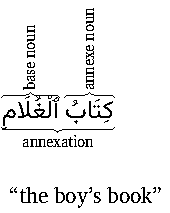
\includegraphics{A-Learners-Grammar-of-Classical-Standard-Arabic_files/figure-latex/unnamed-chunk-12-1.pdf}

The annexation construction consists of two nouns:

\begin{enumerate}
\def\labelenumi{\arabic{enumi}.}
\tightlist
\item
  The \emph{annexe} noun: This is the first noun in the annexation.
\item
  The \emph{base} noun: This is the second noun in the annexation.
\end{enumerate}

The annexe noun \foreignlanguage{arabic}{کِتَاب} is annexed to, and belongs to, the base noun \foreignlanguage{arabic}{ٱَلْغُلَام}.
You can use the alphabetical order (A,~B) to help you remember that the \textbf{a}nnexe noun comes before the \textbf{b}ase noun.

\section{State of the annexe and base nouns}\label{state-of-the-annexe-and-base-nouns}

The base noun in an annexation is always in the i-state. The annexe noun may be in any state, depending on its function in the sentence. For example,

\foreignlanguage{arabic}{کِتَابُ ٱلْغُلَامِ ثَقِيلٌ.}\\
\enquote{The boy's book is heavy.}\\
(The annexe noun is in the u-state.)

\foreignlanguage{arabic}{أَخَذَتِ ٱلْجَارِيَةُ کِتَابَ ٱلْغُلَامِ.}\\
\enquote{The girl took the boy's book.}\\
(The annexe noun is in the a-state.)

\foreignlanguage{arabic}{کَتَبَ ٱلْمُعَلِّمُ فِي کِتَابِ ٱلْغُلَامِ.}\\
\enquote{The teacher\textsubscript{m} wrote in the boy's book.}\\
(The annexe noun is in the i-state.)

\section{Definiteness of the annexation}\label{definiteness-of-the-annexation}

Consider again the annexation expression we have been using so far:

\foreignlanguage{arabic}{کِتَابُ ٱلْغُلَامِ}\\
\enquote{the boy's book}

The base noun \foreignlanguage{arabic}{ٱَلْغُلَام} is definite because it is prefixed by \foreignlanguage{arabic}{ٱَلْ} \enquote{the}.
Therefore we have translated it as \enquote{the boy}.
The annexe noun \foreignlanguage{arabic}{کِتَاب} is not made definite by \foreignlanguage{arabic}{ٱَلْ}.
Nor is it made indefinite by nūnation.
Rather, its definiteness is determined by the base noun.
Because the base noun \foreignlanguage{arabic}{ٱَلْغُلَام} is definite, therefore the annexe noun \foreignlanguage{arabic}{کِتَاب} is also definite.
The entire annexation is definite.

Consider now the case when the base noun is indefinite.

\foreignlanguage{arabic}{کِتَابُ غُلَامٍ}\\
\enquote{a boy's book}

In the above example, the base noun \foreignlanguage{arabic}{غُلَامٍ} is indefinite because it is nūnated and because it does not prefixed by \foreignlanguage{arabic}{ٱَلْ}. Therefore we have translated it as \enquote{a boy}.
The annexe noun \foreignlanguage{arabic}{کِتَاب} is neither nūnated, nor does it have \foreignlanguage{arabic}{ٱَلْ}.
Its definiteness is, again, determined by the base noun.
Because the base noun \foreignlanguage{arabic}{غُلَامٍ} is indefinite, therefore the annexe noun \foreignlanguage{arabic}{کِتَاب} is also indefinite.
The entire annexation is indefinite.

We will see soon, if Allāh wills, why the definiteness of the annexe noun is important.

Here are some examples of definite and indefinite annexations.

\foreignlanguage{arabic}{لَبِسَ ٱلطِّفْلُ قَمِيصَ رَجُلٍ.}\\
\enquote{The child wore \emph{a} man's shirt.}

\foreignlanguage{arabic}{أَخَذَ أَمِيرُ ٱلْجَيْشِ رَايَةَ ٱلْمَلِکِ وَرَفَعَهَا.}\\
\enquote{\emph{The} army's commander took \emph{the} king's flag and raised it.}

\foreignlanguage{arabic}{جَلَسَ ٱلرَّجُلُ فِي ظِلِّ شَجَرَةٍ.}\\
\enquote{The man sat in \emph{a} tree's shade.}

\subsection{\texorpdfstring{Translating the annexation using \enquote{of}}{Translating the annexation using ``of''}}\label{translating-the-annexation-using-of}

So far we have been using the English \enquote{'s} to translate the Arabic annexation. Examples:

\foreignlanguage{arabic}{بَيْتُ رَجُلٍ}\\
\enquote{a man's house}

\foreignlanguage{arabic}{بَيْتُ ٱلرَّجُلِ}\\
\enquote{the man's house}

Instead of using \enquote{'s} we may use \enquote{of} as well. For example:

\foreignlanguage{arabic}{بَيْتُ رَجُلٍ}\\
\enquote{a/the house of a man}

\foreignlanguage{arabic}{بَيْتُ ٱلرَّجُلِ}\\
\enquote{a/the house of the man}

Note that the annexe noun \enquote{house} may be prefixed with either \enquote{a} or \enquote{the}. This will depend on what is more natural in English. Often time both will fit. Here are some examples:

\foreignlanguage{arabic}{لَبِسَ ٱلطِّفْلُ قَمِيصَ رَجُلٍ.}\\
\enquote{The child wore a/the shirt of a man.}

\foreignlanguage{arabic}{أَخَذَ أَمِيرُ ٱلْجَيْشِ رَايَةَ ٱلْمَلِکِ وَرَفَعَهَا.}\\
\enquote{\emph{The} commander of the army took \emph{the} flag of the king and raised it.}

\foreignlanguage{arabic}{جَلَسَ ٱلرَّجُلُ فِي ظِلِّ شَجَرَةٍ.}\\
\enquote{The man sat in \emph{the} shade of a tree.}

\foreignlanguage{arabic}{فَتَحَ ٱلِّصُّ شُبَّاکَ ٱلْبَيْتِ وَدَخَلَ ٱلْبَيْتَ.}\\
\enquote{The thief opened \emph{a/the} window of the house and entered the house.}

It is important to understand that translating the annexe noun into English with \enquote{a} or \enquote{the} is purely for the reason of obtaining a natural translation. This does not affect whether or not the annexe noun is grammatically considered definite in Arabic.

As we mentioned earlier, the definiteness of the annexe noun in Arabic depends only on the definiteness of the base noun.
If the base noun is definite then the annexe noun shall be considered definite as well.
And if the base noun is indefinite then the annexe noun shall be considered indefinite as well.

The need to maintain this distinction will become apparent in the next section.

If the base noun is definite, and it is desired to make the annexe noun grammatically indefinite, then it is necassary to break the annexation, and use a prepositional phrase instead, usually with the preposition \foreignlanguage{arabic}{لِ}, which, here, will mean \enquote{of}. Example:

\foreignlanguage{arabic}{ذَهَبَ ٱلْغُلَامُ إِلَىٰ بَيْتٍ لِلرَّجُلِ.}\\
\enquote{The boy went to a house of the man.}

\foreignlanguage{arabic}{فَتَحَ ٱلِّصُّ شُبَّاکًّا مِنَ ٱلْبَيْتِ وَدَخَلَ ٱلْبَيْتَ.}\\
\enquote{The thief opened a window of the house and entered the house.}

\section{\texorpdfstring{Broken plurals and \emph{āt} sound plurals in annexations}{Broken plurals and āt sound plurals in annexations}}\label{broken-plurals-and-at-sound-plurals-in-annexations}

There is no special rules for broken plurals and \emph{āt} sound plurals in annexations. They behave just like singular nouns. Remember only that \emph{āt} plurals end with \emph{◌ٍ} and \foreignlanguage{arabic}{◌ِ} in the a-state. Here are some examples:

\foreignlanguage{arabic}{حَيَوَانَاتُ ٱلْغَابَةِ وَحْشَةٌ.}\\
\enquote{The animals of the forest are wild.}

\foreignlanguage{arabic}{قَرَأَتْ طَالِبَاتُ ٱلْمَدْرَسَةِ صَفَحَاتِ ٱلْکُتُبِ}\\
\enquote{The school's students\textsubscript{f} read the pages of the books.}

\foreignlanguage{arabic}{فِي ٱلْخِزَانَةِ أَقْلَامُ مُعَلِّمَاتٍ.}\\
``In the cupboard are teachers'\textsubscript{f} pens.

Contrary to broken plurals and \emph{āt} plurals, duals and \emph{ūn} sound plurals behave differently in annexations. We will deal with them in section~\ref{duals-and-sound-un-plurals-in-annexations}

\section{Describers in an annexation}\label{describers-in-an-annexation}

\subsection{Describing the base noun}\label{describing-the-base-noun}

Consider the following expression:

\foreignlanguage{arabic}{کِتَابُ ٱلْجَارِيَةِ}\\
\enquote{the girl's book}

Now say that we want to form an descriptive noun-phrase \enquote{the small girl's book}.
Basically, we want to describe the base noun \foreignlanguage{arabic}{ٱَلْجَارِيَة} \enquote{the girl} with the adjectival noun \foreignlanguage{arabic}{صَغِير} \enquote{a small one}.
Here is how we will express this in Arabic:

\foreignlanguage{arabic}{کِتَابُ ٱلْجَارِيَةِ ٱلصَّغِيرَةِ}\\
\enquote{the small girl's book}

In the manner we are already familiar with, we place the describer \foreignlanguage{arabic}{صَغِير} \enquote{a small one} after the describee
\foreignlanguage{arabic}{ٱَلْجَارِيَة} \enquote{the girl}
and match the describer with the describee in definiteness, state, gender and number (singular, dual, or plural).

Similarly, if we had an indefinite annexation, we would get:

\foreignlanguage{arabic}{کِتَابُ جَارِيَةٍِ صَغِيرَةٍ}\\
\enquote{a small girl's book}

Here are some more examples:

\foreignlanguage{arabic}{لَعِبَتِ ٱلْجَارِيَةُ فِي حَدِيقَةِ ٱلْبَيْتِ ٱلْکَبِيرِ.}\\
\enquote{The girl played in the garden of the big house.}

\foreignlanguage{arabic}{قَرَأَ ٱلْغُلَامُ سُورَةَ ٱلْقُرْآنِ ٱلْکَرِيمِ.}\\
\enquote{The boy read the sūrah of the Noble Qurʾān.}

\foreignlanguage{arabic}{جَلَسَ ٱلرَّجُلُ فِي ظِلِّ شَجَرَةٍ عَرِيضَةٍ وَسِيعَةٍ.}\\
\enquote{The man sat in the shade of a wide broad tree.}

\subsection{Describing the annexe noun}\label{describing-the-annexe-noun}

Consider, again, the same annexation:

\foreignlanguage{arabic}{کِتَابُ ٱلْجَارِيَةِ}\\
\enquote{the girl's book}

Say, now, that we want to describe the annexe noun \foreignlanguage{arabic}{کِتَاب} \enquote{book} with the adjectival noun \foreignlanguage{arabic}{صَغِير} \enquote{a small one}. Normally, nothing can come between the annexe noun and the base noun in an annexation. So, the describer needs to be placed, again, after the base noun.
However, this time it will match the annexe noun, not the base noun, in state, definiteness, gender, and number. So we get:

\foreignlanguage{arabic}{کِتَابُ ٱلْجَارِيَةِ ٱلصَّغِيرُ}\\
\enquote{the girl's small book}

Note how the describer
\foreignlanguage{arabic}{ٱَلصَّغِيرُ} matches the annexe noun \foreignlanguage{arabic}{کِتَابُ} in state and gender.
Note also how the describer is definite with an \foreignlanguage{arabic}{ٱَلْ}. This is because it is matching the annexe noun \foreignlanguage{arabic}{کِتَابُ} in definiteness.
The annexe noun \foreignlanguage{arabic}{کِتَاب} is definite, not with \foreignlanguage{arabic}{ٱَلْ}, but rather because of the definite base noun \foreignlanguage{arabic}{ٱَلْجَارِيَةِ} \enquote{the girl}.
We've already learned this rule in
section~\ref{definiteness-of-the-annexation}
above.

Similarly, if we describe the annexe noun \foreignlanguage{arabic}{کِتَاب} in an indefinite annexation, we get:

\foreignlanguage{arabic}{کِتَابُ جَارِيَةٍ صَغِيرٌ}\\
\enquote{a girl's small book}

This time
the describer
\foreignlanguage{arabic}{صَغِيرٌ}
is indefinite with a nūnated \emph{u}-mark \foreignlanguage{arabic}{◌ٌ}.
This is because
the annexe noun \foreignlanguage{arabic}{کِتَابُ} is indefinite. It is indefinite because base noun \foreignlanguage{arabic}{جَارِيَةٍ} \enquote{a girl} is indefinite.

Now, you might be foreseeing a problem. What if the annexe noun and the base noun have the same gender, and the annexe too is in the i-state? For example, in the sentence:

\foreignlanguage{arabic}{ذَهَبَ ٱلْغُلَامُ إِلَىٰ بَيْتِ ٱلرَّجُلِ ٱلْکَبِيرِ.}\\
\enquote{The boy went to the big/old man's house.}\\
or\\
\enquote{The boy went to the man's big house.}

How do we know whether the describer \foreignlanguage{arabic}{کَبِير} is meant to describe the annexe noun \foreignlanguage{arabic}{بَيْتِ} or the base noun \foreignlanguage{arabic}{ٱَلرَّجُل}?
The annexe noun \foreignlanguage{arabic}{بَيْتِ} and the base noun \foreignlanguage{arabic}{ٱَلرَّجُل} are both masculine, singular, definite, and in the i-state.

The answer is that in such cases, context will have to be clear to tell us which of the two meanings is intended.
If the context makes it clear then there is no harm in using such a sentence for either of the two meanings.

Also, sometimes, the meaning of the describer is such that it will likely apply to only one of the two nouns. For example,

\foreignlanguage{arabic}{ذَهَبَ ٱلْغُلَامُ إِلَىٰ بَيْتِ ٱلرَّجُلِ ٱلْکَرِيمِ.}\\
\enquote{The boy went to a noble/generous man's house.}

In the sentence above the describer \foreignlanguage{arabic}{کَرِيم} \enquote{noble/generous} is likely to apply to a man, and not to a house.

If, however, the context is not clear, and the meaning of the describer can apply to both the annexe noun and the base noun, then the describer is likely to apply to the base noun and not to the annexe noun. So then, this interpretation is more likely:

\foreignlanguage{arabic}{ذَهَبَ ٱلْغُلَامُ إِلَىٰ بَيْتِ ٱلرَّجُلِ ٱلْکَبِيرِ.}\\
\enquote{The boy went to the big/old man's house.}

In order to apply a describer to the annexe noun in such a case, it is better to break the annexation and form a prepositional phrase instead, usually with the preposition \foreignlanguage{arabic}{لِ}, which, here, will mean \enquote{of}. Example:

\foreignlanguage{arabic}{ذَهَبَ ٱلْغُلَامُ إِلَىٰ ٱلْبَيْتِ ٱلْکَبِيرِ لِلرَّجُلِ .}\\
\enquote{The boy went to the big house of the man.}

Here are some more examples:

\foreignlanguage{arabic}{لَعِبَتِ ٱلْجَارِيَةُ بِکُرَةِ ٱلْغُلَامِ ٱلْحَمرَاءِ.}\\
\enquote{The girl played with the boy's red ball.}\\
(Note that \foreignlanguage{arabic}{حَمْرَاء} feminine to match \foreignlanguage{arabic}{کُرَة}.)

\foreignlanguage{arabic}{سَقَطَتْ وَرَقَةُ ٱلشَّجَرَةِ ٱلْخَضْرَاءُ عَلَىٰ مَاءِ ٱلنَّعْرِ ٱلْعَرِيضِ.}\\
\enquote{The green leaf of the tree fell on the water of the broad river.}\\
(Note that \foreignlanguage{arabic}{خَضْرَاء} is in the u-state to match \foreignlanguage{arabic}{وَرَقَة})

\foreignlanguage{arabic}{حَمَلَ ٱلْغُلَامُ حَقِيبَةَ ٱلْمَدْرَسَةِ ٱلثَّقِيلَةَ.}\\
\enquote{The boy carried the heavy school-bag.}\\
(literally: the heavy bag of the school).

\foreignlanguage{arabic}{کَتَبَ ٱلرَّجُلُ عَلَىٰ صَفْحَةِ کِتَابٍ بَيْضَاءَ.}\\
\enquote{The man wrote on the white page of a book.}\\
(Note that \foreignlanguage{arabic}{بَيْضَاءَ} is feminine to match \foreignlanguage{arabic}{صَفْحَة}. However, also note that it has an a-mark \foreignlanguage{arabic}{◌َ} in the i-state because it is semi-flexible.)

\section{Semi-flexible nouns in an annexation}\label{semi-flexible-nouns-in-an-annexation}

Remember that semi-flexible nouns are not nūnated and that when indefinite, their i-state is indicated by an \emph{a}-mark \foreignlanguage{arabic}{◌َ}.
But when definite with \foreignlanguage{arabic}{ٱَلْ} then they behave just like fully-flexible nouns.
Example of the semi-flexible noun
\textsuperscript{2}\foreignlanguage{arabic}{صَحْرَاء} \enquote{a desert}:

\begin{longtable}[]{@{}lll@{}}
\toprule\noalign{}
State & Indefinite & Definite \\
\midrule\noalign{}
\endhead
\bottomrule\noalign{}
\endlastfoot
u-state & \foreignlanguage{arabic}{صَحْرَاءُ} & \foreignlanguage{arabic}{ٱَلصَّحْرَاءُ} \\
a-state & \foreignlanguage{arabic}{صَحْرَاءَ} & \foreignlanguage{arabic}{ٱَلصَّحْرَاءَ} \\
i-state & \foreignlanguage{arabic}{صَحْرَاءَ} & \foreignlanguage{arabic}{ٱَلصَّحْرَاءِ} \\
\end{longtable}

We will now see how semi-flexible nouns behave in an annexation.

\subsection{A semi-flexible noun as the base noun}\label{a-semi-flexible-noun-as-the-base-noun}

Here are examples of the semi-flexible noun \textsuperscript{2}\foreignlanguage{arabic}{صَحْرَاء} \enquote{a desert} as the base noun in an annexation:

\foreignlanguage{arabic}{ٱَلْقَرْيَةُ فِي وَسَطِ ٱلصَّحْرَاءِ.}\\
\enquote{The village is in the middle of the desert.}

\foreignlanguage{arabic}{شَرِبَ ٱلْأَعْرَابِيُّ مَاءً مِنْ بِئْرِ صَحْرَاءَ.}\\
\enquote{The bedouin drank some water from a desert's well.}

As you can see, when
\textsuperscript{2}\foreignlanguage{arabic}{صَحْرَاء}
is definite, then its i-state is indicate by an \emph{i}-mark \foreignlanguage{arabic}{◌ِ}, just like fully-flexible nouns.
However, when it is indefinite, then
its i-state is indicate by an \emph{a}-mark \foreignlanguage{arabic}{◌َ}.

This is consistent with the general behavior of semi-flexible nouns that we are familiar with.

\subsection{A semi-flexible noun as the annexe noun}\label{a-semi-flexible-noun-as-the-annexe-noun}

Contrary from expected behavior, a semi-flexible annexe noun, even when indefinite, takes an \emph{i}-mark~\foreignlanguage{arabic}{◌ِ} in the i-state instead of an \emph{a}-mark~\foreignlanguage{arabic}{◌َ}. Example,

\foreignlanguage{arabic}{قَدِمَ ٱلْأَعْرَابِيُّ مِنْ صَحْرَاءِ أَرْضٍ بَعِيدَةٍ.}\\
\enquote{The bedouin came from the desert of a far land.}

In the above example,
\textsuperscript{2}\foreignlanguage{arabic}{صَحْرَاء} \enquote{a desert} is indefinite because it is the annexe noun to an indefinite base noun \foreignlanguage{arabic}{أَرْض} \enquote{a land}.
It is in the i-state because it is preceded by the preposition \foreignlanguage{arabic}{مِنْ} \enquote{from}.
Nevertheless, it takes an \emph{i}-mark \foreignlanguage{arabic}{مِنْ صَحْرَاءِ أَرْضٍ}, not an \emph{a}-mark, which would be incorrect: \(\times\)~\foreignlanguage{arabic}{مِنْ صَحْرَاءَ أَرْضٍ}.

\section{Annexations with more than two nouns}\label{annexations-with-more-than-two-nouns}

So far we have seen annexations with two nouns. Annexations may be arbitrarily long. Here is an example of a noun-chain with more than two nouns:

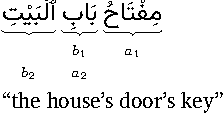
\includegraphics{A-Learners-Grammar-of-Classical-Standard-Arabic_files/figure-latex/unnamed-chunk-13-1.pdf}

The above annexation consists of three nouns. It may be divided into two sub-annexations:

\begin{enumerate}
\def\labelenumi{\roman{enumi}.}
\tightlist
\item
  \foreignlanguage{arabic}{مِفْتَاحُ بَابِ} \enquote{door's key}. Its annexe noun \(a_1\)~is \foreignlanguage{arabic}{مِفْتَاح} and its base noun~\(b_1\) is \foreignlanguage{arabic}{بَابِ}.
\item
  \foreignlanguage{arabic}{بَابِ ٱلْبَيْتِ} \enquote{the house's door}. Its annexe noun \(a_2\)~is \foreignlanguage{arabic}{بَابِ} and its base noun~\(b_2\) is \foreignlanguage{arabic}{ٱلْبَيْتِ}.
\end{enumerate}

The noun \foreignlanguage{arabic}{بَاب} \enquote{door} is common to both sub-annexations. It is the base noun of the first sub-annexation
\foreignlanguage{arabic}{مِفْتَاحُ بَابِ} \enquote{door's key}.
At the same time, it is also the annexe noun of the second sub-annexation
\foreignlanguage{arabic}{بَابِ ٱلْبَيْتِ} \enquote{the house's door}.

Only the final base noun may have \foreignlanguage{arabic}{ٱَلْ} or be nūnated. If the final base noun has \foreignlanguage{arabic}{ٱَلْ} (as above) then all the nouns in the annexation are definite.

And if the final base noun is indefinite, as in the example below, then all the nouns in the annexation are indefinite.

\foreignlanguage{arabic}{مِفْتَاحُ بَابِ بَيْتٍ}\\
\enquote{a house's door's key}

All the nouns except the first annexe noun must be in the i-state. Consistent with
section~\ref{a-semi-flexible-noun-as-the-annexe-noun}
if a semi-flexible noun is any of the annexe nouns and is in the i-state, then its i-state is indicated by an \emph{a}-mark \foreignlanguage{arabic}{◌َ}. Example:

\foreignlanguage{arabic}{مِنْ بِئْرِ صَحْرَاءِ أَرْضٍ}\\
\enquote{from the well of the desert of a land}

\section{Pronouns as base nouns}\label{pronouns-as-base-nouns}

Consider the expression:

\enquote{his book}

This expression is very similar to the annexation:

\foreignlanguage{arabic}{کِتَابُ ٱلْغُلَامِ}\\
\enquote{the boy's book}

The difference is that we would like to replace the base noun \foreignlanguage{arabic}{ٱَلْغُلَام} \enquote{the boy} with the pronoun \enquote{his}. For this we use the attached pronoun \foreignlanguage{arabic}{هُ}. When we place this pronoun as the base noun, we get:

\foreignlanguage{arabic}{کِتَابُهُ}\\
\enquote{his book}

This annexation follows the same rules as the other annexations we have been studying so far:

\begin{itemize}
\tightlist
\item
  The annexe noun may be in any state, depending on its function in the sentence.
\item
  The base noun is in the i-state. But because the base noun is a pronoun, and pronouns are rigid nouns (see section~\ref{rigidity-of-pronouns} that don't change their ending based on their state, therefore it's i-state will not be apparent.
\end{itemize}

Here are some examples of this annexation used in sentences:

\foreignlanguage{arabic}{کِتَابُهُ ثَقِيلٌ.}\\
\enquote{His book is heavy}

\foreignlanguage{arabic}{قَرَأَ ٱلرَّجُلُ کِتَابَهُ.}\\
\enquote{The man read his book.}

\foreignlanguage{arabic}{کَتَبَ ٱلْمُعَلِّمُ فِي کِتَابهِ.}\\
\enquote{The teacher\textsubscript{m} wrote in his book.}

If the annexe noun ends with \foreignlanguage{arabic}{ة} then it is converted to a \foreignlanguage{arabic}{ت} when annexing it to an attached pronoun. For example:

\foreignlanguage{arabic}{ذَهَبُوا إِلَىٰ مَدْرَسَتِهِمْ.}\\
\enquote{They went to their school.}

Here are some more examples of annexing to the different attached pronouns:

\foreignlanguage{arabic}{دَخَلْتَ بَيْتَکَ.}\\
\enquote{You\textsubscript{1,m} entered your\textsubscript{1,m} house.}

\foreignlanguage{arabic}{أَکَلَتَا طَعَامَهُمَا.}\\
\enquote{They\textsubscript{2,f} ate their\textsubscript{2} food.}

\foreignlanguage{arabic}{قَدِمْتُ إِلَىٰ مَدِينَتِکُمْ}\\
\enquote{I have arrived to your\textsubscript{3,m} city.}

\foreignlanguage{arabic}{هُوَ إِمَامُ مَسْجِدِنَا.}\\
\enquote{He is the ʾImām of our mosque.}

If the annexe noun is semi-flexible then it gets a \foreignlanguage{arabic}{◌ِ} in the i-state, as we've already learned. Example with the semi-flexible broken plural \textsuperscript{2}\foreignlanguage{arabic}{حَدَائِق} \enquote{gardens}.

\foreignlanguage{arabic}{لَعِبْنَ فِي حَدَائِقِهِنَّ.}\\
\enquote{They\textsubscript{3,f} played in their\textsubscript{3,f} gardens.}

If an annexe noun ends with \foreignlanguage{arabic}{ىٰ} then it gets converted to an \foreignlanguage{arabic}{أَلِف} when annexing it to an attached pronoun. Example with \textsuperscript{2}\foreignlanguage{arabic}{فَتَاوَىٰ} \enquote{legal opinions}:

\foreignlanguage{arabic}{کَتَبَ تَلَامِذَةُ ٱلشَّيْخِ فَتَاوَاهُ فِي کُتُبِهِمْ.}\\
\enquote{The pupils of the religious scholar wrote down his legal opinions in their books.}

For the singular speaker-participant there are two variants for the attached pronoun:

\begin{enumerate}
\def\labelenumi{\roman{enumi}.}
\tightlist
\item
  \foreignlanguage{arabic}{ي} \emph{-ī}
\item
  \foreignlanguage{arabic}{يَ} \emph{-ya}
\end{enumerate}

The first (\foreignlanguage{arabic}{ي} \emph{-ī}) is more commonly used. Example:

\foreignlanguage{arabic}{قَرَأْتُ کِتَابِي}\\
\enquote{I read my book.}

\foreignlanguage{arabic}{أَقْلَامِي قَصِيرَة.}\\
\enquote{My pens are short.}

If, however, the annexe noun ends in a long vowel or a semi-vowel then
(\foreignlanguage{arabic}{ي} \emph{-ī}) is disallowed and only
(\foreignlanguage{arabic}{يَ} \emph{-ya}) shall be used.
Example with the semi-flexible broken plural \textsuperscript{2}\foreignlanguage{arabic}{هَدَايَا} \enquote{gifts}:

\foreignlanguage{arabic}{أَعْجَبَتْهُمْ هَدَايَايَ.}\\
\enquote{My gifts pleased them.}

\subsection{Describers with annexations to pronouns}\label{describers-with-annexations-to-pronouns}

Consider the annexation:

\foreignlanguage{arabic}{کِتَابُهُ}\\
\enquote{his book}

The annexe noun is \foreignlanguage{arabic}{کِتَاب} and the base noun is the pronoun \foreignlanguage{arabic}{ه}.
We would like add a describer to this expression.
Remember from section~\ref{definiteness-of-pronouns} that pronouns are definite nouns. That makes the annexe noun \foreignlanguage{arabic}{کِتَاب} also definite.
Therefore, any describer for this annexation will need to be definite too.

Here is a new rule: Pronouns may not be describees. That is: they are not allowed to have describers.
Even in English you may say:

\enquote{The good boy went.}

but you can't say:

\(\times\)~\enquote{The good \emph{he} went.}

So, any describers for the annexation must necessarily only describe the annexe noun, not the base pronoun. Example:

\foreignlanguage{arabic}{کِتَابُهُ الأَحْمَرُ}\\
\enquote{his red book}

Here are some more examples:

\foreignlanguage{arabic}{کَتَبْتُ بِقَلَمِيَ ٱلْأَسْوَدِ}\\
\enquote{I wrote with my black pen.}

\foreignlanguage{arabic}{حَمَلَ غِلْمَانُ ٱلْقَرْيَةِ حَقَائبَهُمُ ٱلثَّقِيلَة إِلَىٰ مَدْرَسَتِهِمُ ٱلْبَعِيدَةِ.}\\
\enquote{The village boys carried their heavy bags to their distant school.}\\
(literally: the village's boys.)

\section{\texorpdfstring{Duals and \emph{ūn} sound plurals in annexations}{Duals and ūn sound plurals in annexations}}\label{duals-and-sound-un-plurals-in-annexations}

We have already dealt with broken plurals and \emph{āt} sound plurals in annexations in
section~\ref{broken-plurals-and-at-sound-plurals-in-annexations}.

In this section we will deal with
duals and \emph{ūn} sound plurals in annexations.

\subsection{\texorpdfstring{Duals and \emph{ūn} sound plurals as base nouns}{Duals and ūn sound plurals as base nouns}}\label{duals-and-un-sound-plurals-as-base-nouns}

As base noun, duals and \emph{ūn} sound plurals behave no differently than other nouns. Being base nouns they will be in the i-state and this shall be indicated by:

\begin{enumerate}
\def\labelenumi{\roman{enumi}.}
\tightlist
\item
  \foreignlanguage{arabic}{◌َيْنِ} \emph{-ayni} for duals
\item
  \foreignlanguage{arabic}{◌ِينَ} \emph{-īna} for \emph{ūn} sound plurals
\end{enumerate}

Here are some examples:

\foreignlanguage{arabic}{لَجِئَ ٱلْمَظْلُومُنَ ٱلضُّعَفَاءُ فِي بِلَادِ ٱلْمُسْلِمِينَ ٱلْآمِنَةِ.}\\
\enquote{The weak wronged ones took refuge in the secure lands of the Muslims.}

\foreignlanguage{arabic}{أُخُتُ ٱلْغُلَامَيْنِ ٱلطَّوِيلَيْنِ صَغِيرَةِ.}\\
\enquote{The tall boys'\textsubscript{2} sister is little.}

\foreignlanguage{arabic}{هِيَ طَالِبَةُ مُعَلِّمَتَيْنِ کَرِيمَتَيْنِ.}\\
\enquote{She is the student\textsubscript{f} of noble teachers\textsubscript{2,f}.}

\subsection{\texorpdfstring{Duals and \emph{ūn} sound plurals as annexe nouns}{Duals and ūn sound plurals as annexe nouns}}\label{duals-and-un-sound-plurals-as-annexe-nouns}

When duals and \emph{ūn} sound plurals are annexe nouns, then their final \foreignlanguage{arabic}{ن} is treated as a sort of nūnation and is, therefore, deleted before annexing them to a base noun. For example:

\foreignlanguage{arabic}{بَيْتَا ٱلرَّجُلِ}\\
\enquote{the man's houses\textsubscript{2}}\\
not\\
\(\times\)~\foreignlanguage{arabic}{بَيْتَانِ ٱلرَّجُلِ}

Note, also, that because the base noun \foreignlanguage{arabic}{ٱَلرَّجُلِ} begins with a connecting hamzah \foreignlanguage{arabic}{ٱ}, therefore the long vowel \emph{ā} at the end of \foreignlanguage{arabic}{بَيْتَا} is pronounced as a short vowel \emph{a}, thus:

\emph{bayta -rrajuli}\\
not\\
\(\times\)~\emph{baytā -rrajuli}

If the dual annexe noun were in the i-state then the final \foreignlanguage{arabic}{ي} gets an \emph{i}-mark \emph{◌ِ} if there is following connecting hamzah. Example:

\foreignlanguage{arabic}{قَرَأْتُ کِتَابَيِ ٱلرَّجُلِ.}\\
\emph{qaraʾtu kitābayi -rrajul}\\
\enquote{I read the man's books\textsubscript{2}.}

Here are some more examples including \emph{ūn} sound plurals:

\foreignlanguage{arabic}{مُعَلِّمُو ٱلْغُلَامِ کِرَامٌ.}\\
\emph{muɛallimu -lg͡hulāmi kirām.}\\
\enquote{The boy's teachers\textsubscript{3} are noble.}\\
(Note that there is no silent \foreignlanguage{arabic}{أَلِف} after \foreignlanguage{arabic}{مُعَلِّمُو} as there is after a verb with a plural absentee-participant doer pronoun, e.g.~\foreignlanguage{arabic}{لَعِبُوا} \enquote{they\textsubscript{3,m} played})

\foreignlanguage{arabic}{لَعِبَ ٱبْنَا ٱلرَّجُلِ مَعَ لَاعِبِي مَدِينَتِهِمْ.}\\
\emph{laɛiba -bna -rrajuli maɛa lāɛibī madīnatihim.}\\
\enquote{The man's sons\textsubscript{2} played with the players of their city.}

\subsubsection{\texorpdfstring{Annexing duals and \emph{ūn} sound plurals to pronouns}{Annexing duals and ūn sound plurals to pronouns}}\label{annexing-duals-and-un-sound-plurals-to-pronouns}

Duals and \emph{ūn} sound plurals can be annexed to attached pronouns, and in this case too, they will lose their final \foreignlanguage{arabic}{ن}. Examples:

\foreignlanguage{arabic}{مُعَلِّمُونَا طَيِّبُونَ.}\\
\enquote{Our teachers\textsubscript{3,m} are good.}

\foreignlanguage{arabic}{لَعِبَتِ ٱلْجَارِيَةُ مَعَ صَدِيقَتَيْهَا}\\
\enquote{The girl played with her friends\textsubscript{2,f}.}

\foreignlanguage{arabic}{بَيْتَايَ کَبِيرَانِ.}\\
\enquote{My houses\textsubscript{2} are big.}\\
(Note that only the \foreignlanguage{arabic}{يَ} variant is allowed to be used because of \foreignlanguage{arabic}{بَيْتَا} ending with a long vowel.)

\foreignlanguage{arabic}{قَرَأْتُ کِتَابَيَّ}\\
(Note how \foreignlanguage{arabic}{کِتَابَيْ + يَ} becomes \foreignlanguage{arabic}{کِتَابَيَّ}.)

There are also two special cases in this category and we will examine them below:

\paragraph*{\texorpdfstring{Annexing an \emph{ūn} sound plural to the singular speaker participant pronoun}{Annexing an ūn sound plural to the singular speaker participant pronoun}}\label{annexing-an-un-sound-plural-to-the-singular-speaker-participant-pronoun}
\addcontentsline{toc}{paragraph}{Annexing an \emph{ūn} sound plural to the singular speaker participant pronoun}

When an \emph{ūn} sound plural is annexed to the singular speaker participant pronoun, then again, only the \foreignlanguage{arabic}{يَ} variant can be used. However, in addition, the expression will appear the same regardless of the state of the annexe noun. So for all states (u-state, a-state, and i-state), we will get:

\foreignlanguage{arabic}{مُعَلِّمِيَّ}

We don't say \(\times\)~\foreignlanguage{arabic}{مُعَلِّمُويَ} for the u-state. Examples:

\foreignlanguage{arabic}{مُعَلِّمِيَّ کِرَامٌ.}\\
\enquote{My teachers\textsubscript{3,m} are noble.}\\
(u-state)

\foreignlanguage{arabic}{سَأَلْتُ مُعَلِّمِيَّ}\\
\enquote{I asked my teachers\textsubscript{3,m}.}\\
(a-state)

\foreignlanguage{arabic}{أَخَذْتُ کِتَابًا مِنْ مُعَلِّمِيَّ}\\
\enquote{I took a book from my teachers\textsubscript{3,m}.}\\
(i-state)

\paragraph*{Annexing an dual noun to a dual pronoun}\label{annexing-an-dual-noun-to-a-dual-pronoun}
\addcontentsline{toc}{paragraph}{Annexing an dual noun to a dual pronoun}

When a dual noun is to be annexed to a dual pronoun, then the dual annexe noun is often converted to a plural. For example, instead of saying

\foreignlanguage{arabic}{نَظَرْتُ إِلَىٰ رَأْسَيْهِمَا}
\enquote{I looked at their\textsubscript{2} heads\textsubscript{2}.}

it is in fact, more common, to say

\foreignlanguage{arabic}{نَظَرْتُ إِلَىٰ رُؤُوسِهِمَا}
\enquote{I looked at their\textsubscript{2} heads\textsubscript{3}.}

Although the former is also correct. This is because the annexation of a dual to a dual is considered burdensome upon the tongue to utter, and so the plural is prefered.

\section{\texorpdfstring{Annexations with \enquote{and}}{Annexations with ``and''}}\label{annexations-with-and}

\subsection{Multiple annexe nouns and one base noun}\label{multiple-annexe-nouns-and-one-base-noun}

In English we can have an expression like \enquote{the pen and the book of the boy} = \enquote{the boy's pen and book}. In this sentence there are two annexe nouns and one base noun.

In order to express this in Arabic, we will say:

\foreignlanguage{arabic}{قَلَمُ ٱلْغُلَامِ وَکِتَابُهُ}\\
\emph{qalamu -lg͡hulāmi wa kitābuhu}\\
\enquote{the boy's pen and his book} = \enquote{the boy's pen and book}

Note that the annexation is not broken by the insertion of \foreignlanguage{arabic}{وَ} \emph{wa} \enquote{and}. Rather a second annexation is used and the two are separated by \foreignlanguage{arabic}{وَ} \emph{wa} \enquote{and}. This is the preferred way of expressing such expressions.

There is another, less preferred way of expressing this. And this is by breaking the first annexation and inserting \foreignlanguage{arabic}{وَ} \emph{wa} \enquote{and}:

\foreignlanguage{arabic}{قَلَمُ وَکِتَابُ ٱلْغُلَامِ}\\
\emph{qalamu wa kitābu -lg͡hulāmi}\\
\enquote{the boy's pen and book}

This second method is not considered as eloquent. Some even consider it incorrect. So we advise you to use the first method whenever possible.

\subsubsection{With pronouns}\label{with-pronouns}

If the base noun in the first annexation is replaced with a pronoun then only the first method is allowed. For example,

\foreignlanguage{arabic}{قَلَمُهُ وَکِتَابُهُ}\\
\emph{qalamuhu wakitābuhu}\\
\enquote{his pen and his book}

\subsection{One annexe noun and multiple base nouns}\label{one-annexe-noun-and-multiple-base-nouns}

We can also have expressions like \enquote{the house of the boy and the girl}. In this sentence there is one annexe noun and two base nouns.

To express this in Arabic we will say:

\foreignlanguage{arabic}{بَيْتُ ٱلْغُلَامِ وَٱلْجَارِيَةِ}\\
\emph{baytu -lg͡hulāmi wa-ljāriyati}\\
\enquote{the house of the boy and the girl}

Note that both
\foreignlanguage{arabic}{ٱلْغُلَامِ} \emph{ʾalg͡hulāmi} and \foreignlanguage{arabic}{ٱَلْجَارِيَةِ} \emph{ʾaljāriyati} are in the i-state because they are both base nouns in the annexation.

\subsubsection{With pronouns}\label{with-pronouns-1}

If one or both of the base nouns in the annexation is replaced with a pronoun then the first noun must be repeated. For example,

\foreignlanguage{arabic}{بَيْتُ ٱلْغُلَامِ وَبَيْتُهَا}\\
\enquote{the boy's house and her house}

\foreignlanguage{arabic}{بَيْتُهُ وَبَيْتُهَا}\\
\emph{baytuhu wabaytuhā}\\
\enquote{his house and her house}

\section{Usage of the annexation}\label{usage-of-the-annexation}

\subsection{Primarily belonging}\label{primarily-belonging}

\subsection{\texorpdfstring{\foreignlanguage{arabic}{نحو، مثل، شبه}}{نحو، مثل، شبه}}\label{ux646ux62dux648-ux645ux62bux644-ux634ux628ux647}

Don't become definite when annexed to pronoun

\subsection{\texorpdfstring{\foreignlanguage{arabic}{نفس} \enquote{self}}{نفس ``self''}}\label{ux646ux641ux633-self}

\foreignlanguage{arabic}{ضَرَبا أنفسهما}

\foreignlanguage{arabic}{قالت لِي نَفسي}

\subsection{annexation of material}\label{annexation-of-material}

\foreignlanguage{arabic}{خاتمُ ذَهَبٍ}

\foreignlanguage{arabic}{خاتمٌ ذَهَبٌ}

\foreignlanguage{arabic}{خاتمٌ مِن ذَهَبٍ}

\subsection{\texorpdfstring{\foreignlanguage{arabic}{مَدينَةُ دَمشق}}{مَدينَةُ دَمشق}}\label{ux645ux62fux64aux646ux629-ux62fux645ux634ux642}

\subsection{\texorpdfstring{\foreignlanguage{arabic}{مجرد ترفيه}}{مجرد ترفيه}}\label{ux645ux62cux631ux62f-ux62aux631ux641ux64aux647}

\chapter{Irregular nouns}\label{irregular-nouns}

\section{Introduction}\label{introduction-11}

There are some nouns in Arabic which are \emph{irregular} and behave a little differently than other \emph{regular} nouns. In this chapter we will study these irregular nouns.

\section{The five nouns}\label{the-five-nouns}

There are five nouns in Arabic which are irregular in the same basic way. Collectively, they are called \enquote{the five nouns}.
They behave a little differently from regular nouns in how they display their state.

\subsection{\texorpdfstring{\foreignlanguage{arabic}{أَبٌ} \emph{ʾab}, \foreignlanguage{arabic}{أَخٌ} \emph{ʾak͡h}, and \foreignlanguage{arabic}{حَمٌ} \emph{ḥam}}{أَبٌ ʾab, أَخٌ ʾak͡h, and حَمٌ ḥam}}\label{ux623ux628-eab-ux623ux62e-eax-and-ux62dux645-ham}

The first three nouns that we will talk about are:

\begin{enumerate}
\def\labelenumi{\roman{enumi}.}
\tightlist
\item
  \foreignlanguage{arabic}{أَب} \emph{ʾab} \enquote{a father} (root: \foreignlanguage{arabic}{«أبو»})
\item
  \foreignlanguage{arabic}{أَخ} \emph{ʾak͡h} \enquote{a brother} (root: \foreignlanguage{arabic}{«أخو»})
\item
  \foreignlanguage{arabic}{حَم} \emph{ḥam} \enquote{a father-in-law} (root: \foreignlanguage{arabic}{«حمو»})
\end{enumerate}

The final root letter of all three of these nouns is \foreignlanguage{arabic}{و}. However, irregularly, it is omitted in most formations of the word. It does resurface in some cases as we will describe below.

Without the final root letter \foreignlanguage{arabic}{و}, these nouns display their state like regular nouns. Here are some examples:

\foreignlanguage{arabic}{لِلْجَارِيَةِ أَبٌ کَبِيرٌ وَأَخٌ صَغِيرٌ.}\\
\emph{liljāriyati ʾabun kabīrun waʾak͡hun ṣag͡hīr}\\
\enquote{The girl has an old father and a young brother.}

\foreignlanguage{arabic}{ضَرَبَ ٱلْغُلَامُ أَخًا لَهُ.}\\
\emph{ḍaraba -lg͡hulāmu ʾak͡han lahu.}\\
\enquote{The boy beat a brother of his.}

\foreignlanguage{arabic}{ٱَلْحَمُ وَٱلْأَبُ فِي بَيْتِ ٱلْأَخِ.}\\
\emph{ʾalḥamu walʾabu fī bayti -lʾak͡h.}\\
\enquote{The father-in-law and the father are in the brother's house.}

Where the nouns behave irregularly is when they are an annexe noun in an annexation. Then instead of displaying their state with \foreignlanguage{arabic}{◌ُ}, \foreignlanguage{arabic}{◌َ}, and \foreignlanguage{arabic}{◌ِ}, they display their state using the long vowels \foreignlanguage{arabic}{و} \emph{ū}, \foreignlanguage{arabic}{ا} \emph{ā}, and \foreignlanguage{arabic}{ي} \emph{ī} instead. Here are some examples:

\foreignlanguage{arabic}{هُوَ أَخُو ٱلْجَارِيَةِ.}\\
\emph{huwa ʾak͡hu -ljāriyah}\\
\enquote{He is the girl's brother.}

\foreignlanguage{arabic}{سَأَلْتُ أَبَا صَدِيقِي عَنْ أَمْرٍ.}\\
\emph{saʾaltu ʾabā ṣadīqī ɛan ʾamr.}\\
\enquote{I asked my friend's father about a matter.}

\foreignlanguage{arabic}{ذَهَبْتُ إِلَىٰ بَيْتِ حَمِي ٱلرَّجُلِ.}\\
\emph{d͡hahabtu ʾilā bayti ḥami -rrajul.}\\
\enquote{I went to the man's father-in-law's house.}

When these nouns are annexed to attached pronouns, then in most cases they will behave as above. So, for example,

\foreignlanguage{arabic}{أَبُوهُ}\\
\emph{ʾabūhu}\\
\enquote{his father} (u-state).

\foreignlanguage{arabic}{أَخَانَا}\\
\emph{ʾak͡hānā}\\
\enquote{our brother} (a-state).

However, if the attached pronoun is \foreignlanguage{arabic}{ي} (for the singular speaker participant), then in that case, the attached pronoun \foreignlanguage{arabic}{ي} attaches to the annexe noun directly, without any intervening long vowel:

\foreignlanguage{arabic}{أَخِي}\\
\emph{ʾak͡hī}\\
\enquote{my brother} (u-state, a-state, and i-state).

\foreignlanguage{arabic}{أَبِي}\\
\emph{ʾabī}\\
\enquote{my father} (u-state, a-state, and i-state).

\foreignlanguage{arabic}{حَمِي}\\
\emph{ḥamī}\\
\enquote{my father-in-law} (u-state, a-state, and i-state).

Here are some more examples in sentences:

\foreignlanguage{arabic}{أَخُوهُ طَوِيلٌ وَأَخُوهَا قَصِيرٌ وَأَخِي کَبِيرٌ.}\\
\emph{ʾak͡hūhu ṭawīlun waʾak͡hūhā qaṣīrun waʾak͡hī kabīr.}\\
\enquote{His brother is tall and her brother is short and my brother is big.}

\foreignlanguage{arabic}{سَأَلَ أَخَاهُمْ وَأَخَانَا.}\\
\emph{saʾaltu ʾak͡hāhum waʾak͡hānā.}\\
\enquote{I asked their\textsubscript{m,3+} brother and our brother.}

\foreignlanguage{arabic}{شَکَرَ أَخِي أَبِي.}\\
\emph{s͡hakara ʾak͡hī ʾabī.}\\
\enquote{My brother thanked my father.}

\foreignlanguage{arabic}{ذَهَبْتُ إِلَىٰ بَيْتِ أَخِيهِنَّ.}\\
\emph{d͡hahabtu ʾilā bayti ʾak͡hīhinn.}\\
\enquote{I went to their\textsubscript{f,3+} brother's house.}

The above irregular behavior of these three nouns is only when they are annexe nouns. When they happen to be base nouns in annexations, then they again they behave like regular nouns and their state is displayed by the short vowel marks \foreignlanguage{arabic}{◌ُ}, \foreignlanguage{arabic}{◌َ}, and \foreignlanguage{arabic}{◌ِ}, when definite, and by nūnation
\foreignlanguage{arabic}{◌ٌ},
\foreignlanguage{arabic}{◌ً}, and
\foreignlanguage{arabic}{◌ٍ}, when indefinite.
. Examples:

\foreignlanguage{arabic}{بَيْتُ ٱلْأَخِ کَبِيرٌ.}\\
\emph{baytu -lʾak͡hi kabīr.}\\
\enquote{The brother's house is big.}

\foreignlanguage{arabic}{ذَهَبْتُ إِلَىٰ بَيْتِ أَخٍ.}\\
\emph{d͡hahabtu ʾilā bayti ʾak͡h.}\\
\enquote{I went to a brother's house.}

When these nouns form their duals and plurals, then the final root letter \foreignlanguage{arabic}{و} is resurfaces.
In forming the broken plural, the final root letter \foreignlanguage{arabic}{و}, being a weak letter, sometimes converts to a \foreignlanguage{arabic}{ء}.
The following table shows their duals and plurals.

\begin{longtable}[]{@{}
  >{\raggedright\arraybackslash}p{(\columnwidth - 6\tabcolsep) * \real{0.1538}}
  >{\raggedright\arraybackslash}p{(\columnwidth - 6\tabcolsep) * \real{0.2308}}
  >{\raggedright\arraybackslash}p{(\columnwidth - 6\tabcolsep) * \real{0.3077}}
  >{\raggedright\arraybackslash}p{(\columnwidth - 6\tabcolsep) * \real{0.3077}}@{}}
\toprule\noalign{}
\begin{minipage}[b]{\linewidth}\raggedright
Word
\end{minipage} & \begin{minipage}[b]{\linewidth}\raggedright
Dual (u-state)
\end{minipage} & \begin{minipage}[b]{\linewidth}\raggedright
Dual (a-state and i-state)
\end{minipage} & \begin{minipage}[b]{\linewidth}\raggedright
Plural
\end{minipage} \\
\midrule\noalign{}
\endhead
\bottomrule\noalign{}
\endlastfoot
\foreignlanguage{arabic}{أَب} \emph{ʾab} & \foreignlanguage{arabic}{أَبَوَانِ} \emph{ʾabawāni} & \foreignlanguage{arabic}{أَبَوَيْنِ} \emph{ʾabawayni} & \foreignlanguage{arabic}{آبَاء} \emph{ʾābāʾ} \\
\foreignlanguage{arabic}{أَخ} \emph{ʾak͡h} & \foreignlanguage{arabic}{أَخَوَانِ} \emph{ʾak͡hawāni} & \foreignlanguage{arabic}{أَخَوَيْنِ} \emph{ʾak͡hawayni} & \foreignlanguage{arabic}{إِخْوَة} \emph{ʾik͡hwah}, \foreignlanguage{arabic}{إِخْوَان} \emph{ʾik͡hwān} \\
\foreignlanguage{arabic}{حَم} \emph{ḥam} & \foreignlanguage{arabic}{حَمَوَانِ} \emph{ḥamawāni} & \foreignlanguage{arabic}{حَمَوَيْنِ} \emph{ḥamawayni} & \foreignlanguage{arabic}{أَحْمَاء} \emph{ʾaḥmāʾ} \\
\end{longtable}

One special note regarding the dual \foreignlanguage{arabic}{أَبَوَانِ}/\foreignlanguage{arabic}{أَبَوَيْنِ}: in addition to meaning \enquote{two fathers}, they can also mean \enquote{both parents}, i.e., \enquote{a father and a mother}. Here are examples of these words in sentences:

\foreignlanguage{arabic}{ذَهَبَ ٱلْأَخَوَانِ إِلَى ٱلْمَسْجِدِ.}\\
\emph{d͡hahaba -lʾak͡hawāni fi -lmasjidi.}\\
\enquote{The brothers\textsubscript{2} went to the mosque.}

\foreignlanguage{arabic}{سَأَلْتُ أَخَوَيَّ عَنْ أَمْرٍ}\\
\emph{saʾaltu ʾak͡hawayya ɛan ʾamrin.}\\
\enquote{I asked my brothers\textsubscript{2} about a matter.}

\foreignlanguage{arabic}{شَکَرْتُ لِأَبَوَيْهِ}\\
\emph{s͡hakartu liʾabawayhi.}\\
\enquote{I thanked his parents.}

\subsection{\texorpdfstring{\foreignlanguage{arabic}{ذُو} \emph{d͡hū} and \foreignlanguage{arabic}{ذَات} \emph{d͡hāt}}{ذُو d͡hū and ذَات d͡hāt}}\label{zu}

The fourth irregular noun from \enquote{the five nouns} is the masculine noun \foreignlanguage{arabic}{ذُو} \emph{d͡hū} and its feminine counterpart \foreignlanguage{arabic}{ذَات} and \emph{d͡hāt}. The words \foreignlanguage{arabic}{ذُو} \emph{d͡hū} and \foreignlanguage{arabic}{ذَات} \emph{d͡hāt} mean \enquote{owner of} or \enquote{possessor of}.

So, for example, \foreignlanguage{arabic}{ذُو ٱلْمَالِ} \emph{d͡hu -lmāli} means \enquote{possessor\textsubscript{m} of wealth} or \enquote{wealthy person\textsubscript{m}}. The singular, dual, and plural of \foreignlanguage{arabic}{ذُو} \emph{d͡hū} in all three states is shown in the table below:

\begin{longtable}[]{@{}
  >{\raggedright\arraybackslash}p{(\columnwidth - 6\tabcolsep) * \real{0.2000}}
  >{\raggedright\arraybackslash}p{(\columnwidth - 6\tabcolsep) * \real{0.2667}}
  >{\raggedright\arraybackslash}p{(\columnwidth - 6\tabcolsep) * \real{0.2667}}
  >{\raggedright\arraybackslash}p{(\columnwidth - 6\tabcolsep) * \real{0.2667}}@{}}
\toprule\noalign{}
\begin{minipage}[b]{\linewidth}\raggedright
State
\end{minipage} & \begin{minipage}[b]{\linewidth}\raggedright
Singular
\end{minipage} & \begin{minipage}[b]{\linewidth}\raggedright
Dual
\end{minipage} & \begin{minipage}[b]{\linewidth}\raggedright
Plural
\end{minipage} \\
\midrule\noalign{}
\endhead
\bottomrule\noalign{}
\endlastfoot
u-state & \foreignlanguage{arabic}{ذُو} \emph{d͡hū} & \foreignlanguage{arabic}{ذَوَا} \emph{d͡hawā} & \foreignlanguage{arabic}{ذَوُو} \emph{d͡hawū} \\
a-state & \foreignlanguage{arabic}{ذَا} \emph{d͡hā} & \foreignlanguage{arabic}{ذَوَيْ} \emph{d͡haway} & \foreignlanguage{arabic}{ذَوِي} \emph{d͡hawī} \\
i-state & \foreignlanguage{arabic}{ذِي} \emph{d͡hī} & same as a-state & same as a-state \\
\end{longtable}

The noun \foreignlanguage{arabic}{ذُو} \emph{d͡hū} and its duals and plurals are only ever used as annexe nouns in annexations. Furthermore, they may not be annexed to pronouns. Here are some examples:

\foreignlanguage{arabic}{ٱَلرَّجُلُ ذُو ٱلْمَالِ.}\\
\emph{ʾarrujulu d͡hu -lmāl.}\\
\enquote{The man is the possessor of wealth.} = \enquote{This man is wealthy.}

The word \foreignlanguage{arabic}{ذَات} is the feminine of \foreignlanguage{arabic}{ذُو}. When used as an annexe noun, its states, duals, and plurals are as in the table below:

\begin{longtable}[]{@{}
  >{\raggedright\arraybackslash}p{(\columnwidth - 6\tabcolsep) * \real{0.2000}}
  >{\raggedright\arraybackslash}p{(\columnwidth - 6\tabcolsep) * \real{0.2667}}
  >{\raggedright\arraybackslash}p{(\columnwidth - 6\tabcolsep) * \real{0.2667}}
  >{\raggedright\arraybackslash}p{(\columnwidth - 6\tabcolsep) * \real{0.2667}}@{}}
\toprule\noalign{}
\begin{minipage}[b]{\linewidth}\raggedright
State
\end{minipage} & \begin{minipage}[b]{\linewidth}\raggedright
Singular
\end{minipage} & \begin{minipage}[b]{\linewidth}\raggedright
Dual
\end{minipage} & \begin{minipage}[b]{\linewidth}\raggedright
Plural
\end{minipage} \\
\midrule\noalign{}
\endhead
\bottomrule\noalign{}
\endlastfoot
u-state & \foreignlanguage{arabic}{ذَاتُ} \emph{d͡hātu} & \foreignlanguage{arabic}{ذَوَاتَا} \emph{d͡hawātā} & \foreignlanguage{arabic}{ذَوَاتُ} \emph{d͡hawātu} \\
a-state & \foreignlanguage{arabic}{ذَاتَ} \emph{d͡hāta} & \foreignlanguage{arabic}{ذَوَاتَيْ} \emph{d͡hawātay} & \foreignlanguage{arabic}{ذَوَاتِ} \emph{d͡hawāti} \\
i-state & \foreignlanguage{arabic}{ذَاتِ} \emph{d͡hāti} & same as a-state & same as a-state \\
\end{longtable}

Examples:

\foreignlanguage{arabic}{هَـٰذِهِ ٱلشَّجَرَةُ ذَاتُ ثَمَرٍ کَثِيرٍ.}\\
\emph{hād͡hihi -s͡hs͡hajaratu d͡hātu t͡hamarin kat͡hīrin.}\\
\enquote{This tree is the possessor of much fruit.} = \enquote{This tree is very fruitful.}

As opposed to \foreignlanguage{arabic}{ذُو} which is only an annexe noun, \foreignlanguage{arabic}{ذَات} may be used a noun in its own right. In this case it means \enquote{personality} or \enquote{essence}. This usage is often found in theological or philosophical works. And, as such, unlike \foreignlanguage{arabic}{ذُو} which can't be annexed to attached pronouns, \foreignlanguage{arabic}{ذَات} can be annexed to attached pronouns. Examples:

\subsection{\texorpdfstring{\foreignlanguage{arabic}{فَم} \emph{fam}}{فَم fam}}\label{ux641ux645-fam}

The fifth of \enquote{the five nouns} is \foreignlanguage{arabic}{فَم} \emph{fam} \enquote{a mouth}. It is the most irregular of \enquote{the five nouns}.

In some ways, the word \foreignlanguage{arabic}{فَم} \emph{fam} is regular. It is only irregular when it is a singular annexe noun. Let's first see its regular bahavior.

\foreignlanguage{arabic}{عَلَى ٱلْوَجْهِ فَمٌ وَفِي ٱلْفَمِ لِسَانٌ.}\\
\emph{ɛala -lwajhi famun wafi -lfami lisān}\\
\enquote{On the face is a mouth, and in the mounth is a tongue.}

It is a base noun in an annexation regularly:

\foreignlanguage{arabic}{نَطَقَ لِسَانُ ٱلْفَمِ.}\\
\emph{naṭaqa lisānu -lfam.}\\
\enquote{The mouth's tongue articulated {[}speech{]}.}

It forms duals regularly, which are used in annexations regularly

\foreignlanguage{arabic}{فَمَا ٱلنَّهْرَيْنِ کَبِيرَانِ.}\\
\emph{fama -nnahrayni kabīrāni.}\\
\enquote{The mouths\textsubscript{2} of the rivers\textsubscript{2} are big.}

Let's now see its irregular behavior.

When \foreignlanguage{arabic}{فَم} is a singular annexe noun, then it is usual for it to follow the example of the rest of the five nouns.

Here is how it will appear as a singular annexe noun in the three states:

\begin{longtable}[]{@{}
  >{\raggedright\arraybackslash}p{(\columnwidth - 4\tabcolsep) * \real{0.3333}}
  >{\raggedright\arraybackslash}p{(\columnwidth - 4\tabcolsep) * \real{0.3333}}
  >{\raggedright\arraybackslash}p{(\columnwidth - 4\tabcolsep) * \real{0.3333}}@{}}
\toprule\noalign{}
\begin{minipage}[b]{\linewidth}\raggedright
u-state
\end{minipage} & \begin{minipage}[b]{\linewidth}\raggedright
a-state
\end{minipage} & \begin{minipage}[b]{\linewidth}\raggedright
i-state
\end{minipage} \\
\midrule\noalign{}
\endhead
\bottomrule\noalign{}
\endlastfoot
\foreignlanguage{arabic}{فُو} \emph{fū} & \foreignlanguage{arabic}{فَا} \emph{fā} & \foreignlanguage{arabic}{فِي} \emph{fī} \\
\end{longtable}

Examples of usage:

\foreignlanguage{arabic}{فُو ٱلنَّهْرِ کَبِيرٌ.}\\
\emph{fu -nnahri kabīr.}\\
\enquote{The mouth of the river is big.}

\foreignlanguage{arabic}{فُوهَا جَمِيلٌ.}\\
\emph{fūhā jamīl.}\\
\enquote{Her mouth is beautiful.}

\foreignlanguage{arabic}{فَتَحَ فَاهُ.}\\
\emph{fataḥa fāh.}\\
\enquote{He opened his mouth.}

\foreignlanguage{arabic}{جَعَلَتِ ٱلْأُمُّ لُقْمَةَ طَعَامٍ فِي فِي ٱبْنَتِهَا.}\\
\emph{jaɛalati -lʾummu luqmata ṭaɛāmin fī fi -bnatihā.}\\
\enquote{The mother put a morsel of food in her daughter's mouth.}

When the attached pronoun for the speaking person \foreignlanguage{arabic}{ي} is attached to \foreignlanguage{arabic}{فُو} \emph{fū}, \foreignlanguage{arabic}{فَا} \emph{fā}, or \foreignlanguage{arabic}{فِي} \emph{fī} the combination is always \foreignlanguage{arabic}{فِيَّ} \emph{fiyya} in all three states. Examples:

\foreignlanguage{arabic}{فِيَّ مَفْتُوحٌ.}\\
\emph{fiyya maftūh.}\\
\enquote{My mouth is open.}

\foreignlanguage{arabic}{فَتَحْتُ فِيَّ.}\\
\emph{fataḥtu fiyy.}\\
\enquote{I opened my mouth.}

\foreignlanguage{arabic}{أَکَلْتُ بِفِيَّ.}\\
\emph{ʾakaltu bifiyy.}\\
\enquote{I ate with my mouth.}

In addition to the above irregular behavior, it is permissible, but less common, to treat \foreignlanguage{arabic}{فَم} regularly as an annexe noun in an annexation. So it is permissible to also say:

\foreignlanguage{arabic}{فَمُ ٱلنَّهْرِ کَبِيرٌ.}\\
\emph{famu -nnahri kabīr.}\\
\enquote{The river's mouth is big.}

\foreignlanguage{arabic}{فَمِي مَفْتُوحٌ.}\\
\emph{famī maftūhun.}\\
\enquote{My mouth is open.}

\foreignlanguage{arabic}{فَمُهَا جَمِيلٌ.}\\
\emph{famuhā jamīlun.}\\
\enquote{Her mouth is beautiful.}

\foreignlanguage{arabic}{فَتَحَ فَمَهُ.}\\
\emph{fataḥa famahu.}\\
\enquote{He opened his mouth.}

\foreignlanguage{arabic}{جَعَلَتِ ٱلْأُمُّ لُقْمَةَ طَعَامٍ فِي فَمِ ٱبْنَتِهَا.}\\
\emph{jaɛalati -lʾummu luqmata ṭaɛāmin fī fami -bnatihā.}\\
\enquote{The mother put a morsel of food in her daughter's mouth.}

The other irregularity of \foreignlanguage{arabic}{فَم} \emph{fam} \enquote{a mouth} is that its broken plural is
\foreignlanguage{arabic}{أَفْواه} \emph{ʾafwāh}.

Note that the letter \foreignlanguage{arabic}{م} has not been used to form the broken plural, and instead a \foreignlanguage{arabic}{و}, and a \foreignlanguage{arabic}{ه} are used to form it.

\section{Other irregular nouns}\label{other-irregular-nouns}

There are more nouns that have irregularity in their own ways. We will discuss them below.

\subsection{\texorpdfstring{\foreignlanguage{arabic}{أُولُو} \emph{ʾulū} and \foreignlanguage{arabic}{أُولَات} \emph{ʾulāt}}{أُولُو ʾulū and أُولَات ʾulāt}}\label{ux623ux648ux644ux648-eulu-and-ux623ux648ux644ux627ux62a-eulat}

\foreignlanguage{arabic}{أُولُو} \emph{ʾulū}
(first syllable has a short vowel with a silent \foreignlanguage{arabic}{و})
means \enquote{people\textsubscript{m} of}. It is only used as a masculine plural annexe noun, similar in meaning to
\foreignlanguage{arabic}{ذَوُو} \emph{d͡hawū} which we discussed in section~\ref{zu} above.
There is no singular or dual of this noun.

Here is its form in the different states:

\begin{longtable}[]{@{}ll@{}}
\toprule\noalign{}
u-state & a-and i-state \\
\midrule\noalign{}
\endhead
\bottomrule\noalign{}
\endlastfoot
\foreignlanguage{arabic}{أُولُو} \emph{ʾulū} & \foreignlanguage{arabic}{أُولِي} \emph{ʾulī} \\
\end{longtable}

Example:

\foreignlanguage{arabic}{لِأُولِي ٱلْأَرْحَامِ حُقُوقٌ.}\\
\emph{liʾuli -lʾarḥāmi ḥuqūq.}\\
\enquote{The people of the wombs (i.e.~blood relatives) have rights.}

The feminine counterpart of
\foreignlanguage{arabic}{أُولُو} \emph{ʾulū}
is
\foreignlanguage{arabic}{أُولَات} \emph{ʾulāt} \enquote{women of}.
The first syllable again has a short vowel with a silent \foreignlanguage{arabic}{و}.

\begin{longtable}[]{@{}ll@{}}
\toprule\noalign{}
u-state & a-and i-state \\
\midrule\noalign{}
\endhead
\bottomrule\noalign{}
\endlastfoot
\foreignlanguage{arabic}{أُولَاتُ} \emph{ʾulātu} & \foreignlanguage{arabic}{أُولَاتِ} \emph{ʾulāti} \\
\end{longtable}

\foreignlanguage{arabic}{لِأُولَاتِ ٱلْحَمْلِ حُقُوقٌ عَلَىٰ بُعُولَتِهِنَّ.}\\
\emph{liʾulāti -lḥamli ḥuqūq ɛalā buɛūlatihinn.}\\
\enquote{The women of pregnancy (i.e.~pregnant women) have rights upon their husbands.}

\subsection{\texorpdfstring{\foreignlanguage{arabic}{أُمّ} \emph{ʾumm}}{أُمّ ʾumm}}\label{ux623ux645-eumm}

The noun
\foreignlanguage{arabic}{أُمّ} \emph{ʾumm} \enquote{a mother}
forms two \emph{āt} sound plural variants:

\begin{enumerate}
\def\labelenumi{\roman{enumi}.}
\tightlist
\item
  \foreignlanguage{arabic}{أُمَّهَات} \emph{ʾummahāt}
\item
  \foreignlanguage{arabic}{أُمَّات} \emph{ʾummāt}
\end{enumerate}

The first variant
\foreignlanguage{arabic}{أُمَّهَات} \emph{ʾummahāt}
is more commonly used.
Example:

\foreignlanguage{arabic}{أُمَّاهَاتُ ٱلْغِلْمَانِ طَيِّبَاتٌ.}\\
\emph{ʾummahātu -lg͡hilmāni ṭayyibāt.}\\
\enquote{The boys' mothers are good.}

\subsection{\texorpdfstring{\foreignlanguage{arabic}{سَنَة} \emph{sanah}}{سَنَة sanah}}\label{ux633ux646ux629-sanah}

The noun
\foreignlanguage{arabic}{سَنَة} \emph{sanah} \enquote{a year}
forms both an \emph{āt} sound plural
and an \emph{ūn} sound plural.
(Remember from
section~\ref{applicability-of-the-un-sound-plural}
that a few nouns that don't denote male intelligent beings have \emph{ūn} sound plurals.)

In both plurals, the singular noun is modified irregularly.

\begin{longtable}[]{@{}
  >{\raggedright\arraybackslash}p{(\columnwidth - 6\tabcolsep) * \real{0.2000}}
  >{\raggedright\arraybackslash}p{(\columnwidth - 6\tabcolsep) * \real{0.2667}}
  >{\raggedright\arraybackslash}p{(\columnwidth - 6\tabcolsep) * \real{0.2667}}
  >{\raggedright\arraybackslash}p{(\columnwidth - 6\tabcolsep) * \real{0.2667}}@{}}
\toprule\noalign{}
\begin{minipage}[b]{\linewidth}\raggedright
Singular
\end{minipage} & \begin{minipage}[b]{\linewidth}\raggedright
\emph{āt} sound plural
\end{minipage} & \begin{minipage}[b]{\linewidth}\raggedright
\emph{ūn} sound plural (u-state)
\end{minipage} & \begin{minipage}[b]{\linewidth}\raggedright
\emph{ūn} sound plural (a- and i-states)
\end{minipage} \\
\midrule\noalign{}
\endhead
\bottomrule\noalign{}
\endlastfoot
\foreignlanguage{arabic}{سَنَة} \emph{sanah} & \foreignlanguage{arabic}{سَنَوَات} \emph{sanawāt} & \foreignlanguage{arabic}{سِنُونَ} \emph{sinūna} & \foreignlanguage{arabic}{سِنِينَ} \emph{sinīna} \\
\end{longtable}

Either of the two plurals may be used interchangeably.
Here are some examples:

\subsection{\texorpdfstring{\foreignlanguage{arabic}{مَاء} \emph{māʾ}}{مَاء māʾ}}\label{ux645ux627ux621-mae}

\foreignlanguage{arabic}{مَاء} \emph{māʾ} \enquote{a water} forms its broken plural irregularly: \foreignlanguage{arabic}{مِيَاه} \emph{miyāh} \enquote{waters}.

\subsection{\texorpdfstring{\foreignlanguage{arabic}{شَفَة} \emph{s͡hafah}}{شَفَة s͡hafah}}\label{ux634ux641ux629-cafah}

\foreignlanguage{arabic}{شَفَة} \emph{s͡hafah} \enquote{a lip}
forms its broken plural irregularly: \foreignlanguage{arabic}{شِفَاه} \emph{s͡hifāh} \enquote{lips}.

Also, despite ending in the feminine marker \foreignlanguage{arabic}{ة}, it does not form an \emph{āt} sound plural.

\subsection{\texorpdfstring{\foreignlanguage{arabic}{ٱِبْن} \emph{ʾibn}, \foreignlanguage{arabic}{ٱِبْنَة} \emph{ʾibnah}, and \foreignlanguage{arabic}{بِنْت} \emph{bint}}{ٱِبْن ʾibn, ٱِبْنَة ʾibnah, and بِنْت bint}}\label{ux671ux628ux646-eibn-ux671ux628ux646ux629-eibnah-and-ux628ux646ux62a-bint}

The noun
\foreignlanguage{arabic}{ٱِبْن} \emph{ʾibn} \enquote{a son} is from the root \foreignlanguage{arabic}{«بنو»}.
It has two feminine counterparts:

\begin{enumerate}
\def\labelenumi{\roman{enumi}.}
\tightlist
\item
  \foreignlanguage{arabic}{ٱِبْنَة} \emph{ʾibnah}
\item
  \foreignlanguage{arabic}{بِنْت} \emph{bint}
\end{enumerate}

which mean \enquote{a daughter}.

\foreignlanguage{arabic}{ٱِبْن} \emph{ʾibn} \enquote{a son}
forms both a broken plural
and an \emph{ūn} sound plural.

Its broken plural is \foreignlanguage{arabic}{أَبْنَاء} \emph{ʾabnāʾ} \enquote{sons}.

In forming the
\emph{ūn} sound plural,
the singular noun is modified irregularly:

\begin{longtable}[]{@{}
  >{\raggedright\arraybackslash}p{(\columnwidth - 4\tabcolsep) * \real{0.2727}}
  >{\raggedright\arraybackslash}p{(\columnwidth - 4\tabcolsep) * \real{0.3636}}
  >{\raggedright\arraybackslash}p{(\columnwidth - 4\tabcolsep) * \real{0.3636}}@{}}
\toprule\noalign{}
\begin{minipage}[b]{\linewidth}\raggedright
Singular
\end{minipage} & \begin{minipage}[b]{\linewidth}\raggedright
\emph{ūn} sound plural (u-state)
\end{minipage} & \begin{minipage}[b]{\linewidth}\raggedright
\emph{ūn} sound plural (a- and i-states)
\end{minipage} \\
\midrule\noalign{}
\endhead
\bottomrule\noalign{}
\endlastfoot
\foreignlanguage{arabic}{ٱِبْن} \emph{ʾibn} & \foreignlanguage{arabic}{بَنُونَ} \emph{banūna} & \foreignlanguage{arabic}{بَنِينَ} \emph{banīna} \\
\end{longtable}

The feminine
\foreignlanguage{arabic}{ٱِبْنَة}
and
\foreignlanguage{arabic}{بِنْت}
\enquote{a daughter}
form the irregular \emph{āt} sound plural
\emph{بَنَات} \emph{banāt} \enquote{daughters}.
Note that
\foreignlanguage{arabic}{بَنَات} \emph{banāt}
is not a broken plural from the root \foreignlanguage{arabic}{«بنت»}. Therefore, it obeys the rules of \emph{āt} sound plurals and does not end with \foreignlanguage{arabic}{◌َ} or \foreignlanguage{arabic}{◌ً} in the a-state.

Here are some examples using these nouns:

\subsection{\texorpdfstring{\foreignlanguage{arabic}{نَاس} \emph{nās}, and \foreignlanguage{arabic}{أُنَاس} \emph{ʾunās}}{نَاس nās, and أُنَاس ʾunās}}\label{ux646ux627ux633-nas-and-ux623ux646ux627ux633-eunas}

\foreignlanguage{arabic}{نَاس} \emph{nās}
and
\foreignlanguage{arabic}{أُنَاس} \emph{ʾunās}
are from the root \foreignlanguage{arabic}{«أنس»}.
They both mean \enquote{a people}.

When indefinite, only
\foreignlanguage{arabic}{أُنَاس} \emph{ʾunās}
tends to be used, and
\foreignlanguage{arabic}{نَاس} \emph{nās}
tends to be unused.

When definite, only
\foreignlanguage{arabic}{ٱَلنَّاس} \emph{ʾannās}
tends to be used, and
\foreignlanguage{arabic}{ٱَلْأُنَاس} \emph{ʾalʾunās}
is unused.

Here are some examples using these nouns:

\subsection{\texorpdfstring{The nouns \foreignlanguage{arabic}{ٱِمْرَأ} and \foreignlanguage{arabic}{ٱِمْرَأَة}}{The nouns ٱِمْرَأ and ٱِمْرَأَة}}\label{the-nouns-ux671ux645ux631ux623-and-ux671ux645ux631ux623ux629}

The nouns
\foreignlanguage{arabic}{ٱِمْرَأ} \emph{ʾimraʾ} (masc.) \enquote{a man, a person} and
\foreignlanguage{arabic}{ٱِمْرَأَة} \emph{ʾimraʾah} (fem.) \enquote{a woman}
are quite irregular.

Firstly,
\foreignlanguage{arabic}{ٱِمْرَأَة} \emph{ʾimraʾah} \enquote{a woman}
is, from the perspective, of its meaning, the feminine counterpart of
\foreignlanguage{arabic}{رَجُل} \emph{rajul} \enquote{a man (male human being)}.

\foreignlanguage{arabic}{ٱِمْرَأ} \emph{ʾimraʾ}, on the other hand, only means \enquote{a man} in a general sense. For example, in the sentence \enquote{A man is only as good as his word.} It can also be translated as \enquote{a person}.

Secondly,
\foreignlanguage{arabic}{ٱِمْرَأ} \emph{ʾimraʾ} \enquote{a man, a person} has no plural.
\foreignlanguage{arabic}{نَاس}/\foreignlanguage{arabic}{أُنَاس} \enquote{a people} and \foreignlanguage{arabic}{قَوْم} \enquote{a population} may be used when a plural is required.

\foreignlanguage{arabic}{ٱِمْرَأَة} \emph{ʾimraʾah} \enquote{a woman} irregularly forms the broken plurals
\foreignlanguage{arabic}{نِسَاء} \emph{nisāʾ} and \foreignlanguage{arabic}{نِسْوَة} \emph{niswah} \enquote{women}. The former
(\foreignlanguage{arabic}{نِسَاء} \emph{nisāʾ}) is more commonly used.

Like \foreignlanguage{arabic}{شَفَة} \emph{s͡hafah}
it also, despite ending in the feminine marker \foreignlanguage{arabic}{ة}, does not form an \emph{āt} sound plural.

Thirdly, both nouns are very irregular in how they become definite nouns with \foreignlanguage{arabic}{ٱَلْ}.
When \foreignlanguage{arabic}{ٱَلْ} is prefixed to these nouns to make them definite, they lose the initial connecting hamzah and change their internal vowels. This table shows what we mean:

\begin{longtable}[]{@{}
  >{\raggedright\arraybackslash}p{(\columnwidth - 4\tabcolsep) * \real{0.1944}}
  >{\raggedright\arraybackslash}p{(\columnwidth - 4\tabcolsep) * \real{0.4028}}
  >{\raggedright\arraybackslash}p{(\columnwidth - 4\tabcolsep) * \real{0.4028}}@{}}
\toprule\noalign{}
\begin{minipage}[b]{\linewidth}\raggedright
State
\end{minipage} & \begin{minipage}[b]{\linewidth}\raggedright
Definite of \foreignlanguage{arabic}{ٱِمْرَأ}
\end{minipage} & \begin{minipage}[b]{\linewidth}\raggedright
Definite of \foreignlanguage{arabic}{ٱِمْرَأَة}
\end{minipage} \\
\midrule\noalign{}
\endhead
\bottomrule\noalign{}
\endlastfoot
u-state & \foreignlanguage{arabic}{ٱَلْمَرْءُ} \emph{ʾalmarʾu} & \foreignlanguage{arabic}{ٱَلْمَرْأَةُ} \emph{ʾalmarʾatu} \\
a-state & \foreignlanguage{arabic}{ٱَلْمَرْءَ} \emph{ʾalmarʾa} & \foreignlanguage{arabic}{ٱَلْمَرْأَةَ} \emph{ʾalmarʾata} \\
i-state & \foreignlanguage{arabic}{ٱَلْمَرْءِ} \emph{ʾalmarʾi} & \foreignlanguage{arabic}{ٱَلْمَرْأَةِ} \emph{ʾalmarʾati} \\
\end{longtable}

The masculine noun
\foreignlanguage{arabic}{ٱِمْرَأ} \emph{ʾimraʾ}
has an additional irregularity.
When it is indefinite, it irregularly displays its state, not only on its final letter \foreignlanguage{arabic}{ء}, but also on the letter before it \foreignlanguage{arabic}{ر}.

It is also permissible for it to behave regularly by displaying its state on its final letter only, but this is not as commonly used.

This table shows what we mean:

\begin{longtable}[]{@{}
  >{\raggedright\arraybackslash}p{(\columnwidth - 4\tabcolsep) * \real{0.2979}}
  >{\raggedright\arraybackslash}p{(\columnwidth - 4\tabcolsep) * \real{0.3830}}
  >{\raggedright\arraybackslash}p{(\columnwidth - 4\tabcolsep) * \real{0.3191}}@{}}
\toprule\noalign{}
\begin{minipage}[b]{\linewidth}\raggedright
State
\end{minipage} & \begin{minipage}[b]{\linewidth}\raggedright
Regular indefinite (less common)
\end{minipage} & \begin{minipage}[b]{\linewidth}\raggedright
Irregular indefinite (more common)
\end{minipage} \\
\midrule\noalign{}
\endhead
\bottomrule\noalign{}
\endlastfoot
u-state & \foreignlanguage{arabic}{ٱِمْرَأٌ} \emph{ʾimraʾun} & \foreignlanguage{arabic}{ٱِمْرُؤٌ} \emph{ʾimruʾun} \\
a-state & \foreignlanguage{arabic}{ٱِمْرَءًا} \emph{ʾimraʾan} & \foreignlanguage{arabic}{ٱِمْرَءًا} \emph{ʾimraʾan} \\
i-state & \foreignlanguage{arabic}{ٱِمْرَأٍ} \emph{ʾimraʾin} & \foreignlanguage{arabic}{ٱِمْرِئٍ} \emph{ʾimriʾin} \\
\end{longtable}

Here are some examples of these nouns:

\chapter{Proper nouns}\label{proper-nouns}

\section{Introduction}\label{introduction-12}

Proper nouns are also known as names. Here are some examples of Arabic names:

\begin{longtable}[]{@{}
  >{\raggedleft\arraybackslash}p{(\columnwidth - 6\tabcolsep) * \real{0.2143}}
  >{\raggedright\arraybackslash}p{(\columnwidth - 6\tabcolsep) * \real{0.2857}}
  >{\raggedleft\arraybackslash}p{(\columnwidth - 6\tabcolsep) * \real{0.2143}}
  >{\raggedright\arraybackslash}p{(\columnwidth - 6\tabcolsep) * \real{0.2857}}@{}}
\toprule\noalign{}
\begin{minipage}[b]{\linewidth}\raggedleft
Men's
\end{minipage} & \begin{minipage}[b]{\linewidth}\raggedright
names
\end{minipage} & \begin{minipage}[b]{\linewidth}\raggedleft
Women's
\end{minipage} & \begin{minipage}[b]{\linewidth}\raggedright
names
\end{minipage} \\
\midrule\noalign{}
\endhead
\bottomrule\noalign{}
\endlastfoot
\foreignlanguage{arabic}{مُحَمَّد} & Muḥammad & \textsuperscript{2}\foreignlanguage{arabic}{عَائِشَة} & Ɛāʾis͡hah \\
\foreignlanguage{arabic}{سَعِيد} & Saɛīd & \textsuperscript{2}\foreignlanguage{arabic}{فَاطِمَة} & Faṭimah \\
\foreignlanguage{arabic}{ٱَلْحَسَن} & al-Ḥasan & \textsuperscript{2}\foreignlanguage{arabic}{حَفْصَة} & Ḥafṣah \\
\foreignlanguage{arabic}{ٱَلنُّعْمَان} & al-Nuɛmān & \textsuperscript{2}\foreignlanguage{arabic}{سُمَيَّة} & Sumayyah \\
\textsuperscript{2}\foreignlanguage{arabic}{طَلْحَة} & Ṭalḥah & \textsuperscript{2}\foreignlanguage{arabic}{جَمِيلَة} & Jamīlah \\
\textsuperscript{2}\foreignlanguage{arabic}{أُسَامَة} & Usāmah & \textsuperscript{2}\foreignlanguage{arabic}{زَيْنَب} & Zaynab \\
\textsuperscript{2}\foreignlanguage{arabic}{عُثْمَان} & Ɛut͡hmān & \textsuperscript{2}\foreignlanguage{arabic}{مَرْيَم} & Maryam \\
\textsuperscript{2}\foreignlanguage{arabic}{عُمَر} & Ɛumar & \textsuperscript{2}\foreignlanguage{arabic}{سُعَاد} & Suɛād \\
\textsuperscript{2}\foreignlanguage{arabic}{إِبْرَاهِيم} & Ibrāhīm & \textsuperscript{2}\foreignlanguage{arabic}{أَسْمَاء} & Asmāʾ \\
\foreignlanguage{arabic}{عَبْد ٱللَّـٰه} & Ɛabd Allāh & \textsuperscript{2}\foreignlanguage{arabic}{لَيْلَىٰ} & Laylā \\
\foreignlanguage{arabic}{أَبُو بَکْر} & Abū Bakr & \textsuperscript{2}\foreignlanguage{arabic}{أُمّ حَبِيبَة} & Umm Ḥabībah \\
\end{longtable}

\begin{longtable}[]{@{}
  >{\raggedleft\arraybackslash}p{(\columnwidth - 6\tabcolsep) * \real{0.1818}}
  >{\raggedright\arraybackslash}p{(\columnwidth - 6\tabcolsep) * \real{0.2727}}
  >{\raggedleft\arraybackslash}p{(\columnwidth - 6\tabcolsep) * \real{0.1818}}
  >{\raggedright\arraybackslash}p{(\columnwidth - 6\tabcolsep) * \real{0.3636}}@{}}
\toprule\noalign{}
\begin{minipage}[b]{\linewidth}\raggedleft
Place
\end{minipage} & \begin{minipage}[b]{\linewidth}\raggedright
names
\end{minipage} & \begin{minipage}[b]{\linewidth}\raggedleft
Misc.
\end{minipage} & \begin{minipage}[b]{\linewidth}\raggedright
names
\end{minipage} \\
\midrule\noalign{}
\endhead
\bottomrule\noalign{}
\endlastfoot
\textsuperscript{2}\foreignlanguage{arabic}{مَکَّة} & Makkah & \textsuperscript{2}\foreignlanguage{arabic}{رَمَضَان} & Ramadān (a month) \\
\textsuperscript{2}\foreignlanguage{arabic}{دِمَشْق} & Damascus & \foreignlanguage{arabic}{أُحُد} & Uḥud (a mountain) \\
\textsuperscript{2}\foreignlanguage{arabic}{مِصْر} & Egypt & \foreignlanguage{arabic}{ٱَلنِّيل} & the Nile (a river) \\
\foreignlanguage{arabic}{ٱَلْقَاهِرَة} & Cairo & \foreignlanguage{arabic}{ٱَلْفَاتِحَة} & the Fātiḥah (a sūrah) \\
\foreignlanguage{arabic}{ٱَلْهِنْد} & India & \foreignlanguage{arabic}{ٱَلْجُمُعَة} & Friday \\
\end{longtable}

Note the following points from the list abobe:

\begin{itemize}
\tightlist
\item
  Although some names begin with \foreignlanguage{arabic}{ٱَلْ}, most don't.
\item
  Many names are semi-flexible (indicated by \textsuperscript{2}\foreignlanguage{arabic}{◌}).
\item
  Some names consist of more than a single word, like \foreignlanguage{arabic}{عَبْد ٱللَّـٰه} Ɛabd Allāh
\end{itemize}

We will explain these and more details regarding proper nouns in this chapter.

\section{Definiteness of proper nouns}\label{definiteness-of-proper-nouns}

Proper nouns differ from common nouns and adjectival nouns in a couple of important ways:

\begin{itemize}
\tightlist
\item
  All proper nouns, even if they don't begin with \foreignlanguage{arabic}{ٱَلْ}, are definite.
\item
  A proper noun which does not begin with \foreignlanguage{arabic}{ٱَلْ}, and which is fully-flexible, shall be nūnated, despite being definite.
\end{itemize}

The above points are exemplified in the following sentence:

\foreignlanguage{arabic}{ذَهَبْتُ إِلَىٰ بَيْتِ مُحَمَّدٍ ٱلْکَرِيمِ وَزَيْنَبَ ٱلطَّيِّبَةِ.}\\
\emph{d͡hahabtu ʾilā bayti muḥammadini -lkarīmi wazaynaba -ṭṭayyibah.}\\
\enquote{I went to the house of the noble Muḥammad and the good Zaynab.}

Note the above from the above example:

\begin{itemize}
\tightlist
\item
  \foreignlanguage{arabic}{مُحَمَّدٍ} is fully-flexible so it has a nūnated \emph{i}-mark \foreignlanguage{arabic}{◌ٍ} in the i-state.
\item
  \foreignlanguage{arabic}{زَيْنَبَ} is semi-flexible so it is not nūnated, and instead has an \emph{a}-mark \foreignlanguage{arabic}{◌َ} in the i-state.
\item
  The proper nouns \foreignlanguage{arabic}{مُحَمَّد} and \foreignlanguage{arabic}{زَيْنَب} are describees in descriptive noun phrases.
\item
  Their describers (\foreignlanguage{arabic}{ٱلْکَرِيمِ} and \foreignlanguage{arabic}{ٱلطَّيِّبَةِ.}, respectively) have \foreignlanguage{arabic}{ٱَلْ} to match the definiteness of the definite proper noun describees. Furthermore, they both end with \foreignlanguage{arabic}{◌ِ} because they match the i-state of their describees.
\end{itemize}

\section{Meanings of names}\label{meanings-of-names}

Many names are re-used from common nouns and adjectival nouns with positive meanings. Examples:

\begin{itemize}
\tightlist
\item
  \foreignlanguage{arabic}{مُحَمَّد} Muḥammad \enquote{a highly praised one\textsubscript{m}}
\item
  \foreignlanguage{arabic}{سَعِيد} Saɛīd \enquote{a happy (fortunate) one\textsubscript{m}}
\item
  \foreignlanguage{arabic}{ٱَلْحَسَن} al-Ḥasan \enquote{the good one\textsubscript{m}}
\item
  \foreignlanguage{arabic}{طَلْحَة} Ṭalḥah \enquote{an acacia (tree)}
\item
  \foreignlanguage{arabic}{جَمِيلَة} Jamīlah \enquote{a beautiful one\textsubscript{f}}
\end{itemize}

It is possible for these names to sometimes (technically) cause a sentence to have an ambiguous meaning. For example,

\foreignlanguage{arabic}{جَلَسَ ٱلْحَسَنُ مَعَ سَعِيدٍ.}\\
\emph{jalsa -lhasanu maɛa saɛīd}\\
\enquote{al-Ḥasan sat with Saɛīd.}\\
or\\
\enquote{The good one\textsubscript{m} sat with a happy (fortunate) one\textsubscript{m}.}

Context would tell us whether the proper noun or the common/adjectival noun meaning is intended.

Note however the following sentence:

\foreignlanguage{arabic}{ذَهَبَتْ جَمِيلَةُ إِلَىٰ ٱلْبَيْتِ.}\\
\emph{d͡hahabat jamīlatu ʾila -lbayt.}

This sentence can only be understood to use \foreignlanguage{arabic}{جَمِيلَة} with its proper noun meaning:

\enquote{Jamīlah went to the house.}

This is because \foreignlanguage{arabic}{جَمِيلَة} is semi-flexible as a proper noun and fully-flexible as an adjectival/common noun. If \foreignlanguage{arabic}{جَمِيلَة} were intended to be used with its adjectival/common noun meaning then it would have a nūnated \emph{u}-mark \foreignlanguage{arabic}{◌ٌ} and the sentence would be:

\foreignlanguage{arabic}{ذَهَبَتْ جَمِيلَةٌ إِلَىٰ ٱلْبَيْتِ.}\\
\emph{d͡hahabat jamīlatun ʾila -lbayt.}\\
\enquote{A beautiful one\textsubscript{f} went to the house.}

We will learn why \foreignlanguage{arabic}{جَمِيلَة} is semi-flexible as a proper noun in section~\ref{proper-nouns-ending-with-looped-ta} below.

\section{Flexibility of proper nouns}\label{flexibility-of-proper-nouns}

In this section we will discuss the flexibility of proper nouns.
For now, we will deal only with proper nouns that do not begin with \foreignlanguage{arabic}{ٱَلْ}.
In terms of their flexibility, proper nouns consist of two types:

\begin{enumerate}
\def\labelenumi{\roman{enumi}.}
\tightlist
\item
  Fully-flexible proper nouns.
\item
  Semi-flexible proper nouns.
\end{enumerate}

We will treat each of them below.

\subsection{Fully-flexible proper nouns}\label{fully-flexible-proper-nouns}

For names that don't begin with \foreignlanguage{arabic}{ٱَلْ}, the default assumption is that they are fully-flexible, unless they fall into one of the categories of semi-flexible nouns (which we will study soon).

Examples of fully-flexible names are:

\begin{longtable}[]{@{}
  >{\raggedleft\arraybackslash}p{(\columnwidth - 6\tabcolsep) * \real{0.2143}}
  >{\raggedright\arraybackslash}p{(\columnwidth - 6\tabcolsep) * \real{0.2857}}
  >{\raggedleft\arraybackslash}p{(\columnwidth - 6\tabcolsep) * \real{0.2143}}
  >{\raggedright\arraybackslash}p{(\columnwidth - 6\tabcolsep) * \real{0.2857}}@{}}
\toprule\noalign{}
\endhead
\bottomrule\noalign{}
\endlastfoot
\foreignlanguage{arabic}{مُحَمَّد} & Muḥammad & \foreignlanguage{arabic}{مُعَاذ} & Muɛād͡h \\
\foreignlanguage{arabic}{نُوح} & Nūh & \foreignlanguage{arabic}{سَعْد} & Saɛd \\
\foreignlanguage{arabic}{شُعَيْب} & S͡huɛayb & \foreignlanguage{arabic}{عَمَّار} & Ɛammār \\
\foreignlanguage{arabic}{عَلِيّ} & Ɛalī & \foreignlanguage{arabic}{حَسَّان} & Ḥassān \\
\foreignlanguage{arabic}{زَيْد} & Zayd & \foreignlanguage{arabic}{سَعِيد} & Saɛīd \\
\foreignlanguage{arabic}{أَنَس} & Anas & \foreignlanguage{arabic}{أُحُد} & Uḥud (a mountain) \\
\end{longtable}

These are all masculine names.

Examples of sentences with fully-flexible proper nouns:

\foreignlanguage{arabic}{زَيْدٌ غُلَامٌ طَيِّبٌّ.}\\
\emph{zaydun g͡hulāmun ṭayyib}\\
\enquote{Zayd is a good boy.}

\foreignlanguage{arabic}{شَکَرَ أَنَسٌ عَلِيًّا.}\\
\emph{s͡hakara ʾanasun ɛaliyyā.}\\
\enquote{Anas thanked Ɛalī.}

\foreignlanguage{arabic}{لَبِسَ سَعِيدٌ قَمِيصَ نُوحٍ ٱلأَخْضَرَ.}\\
\emph{labisa saɛīdun qamīṣa nūḥini -lʾak͡hḍar.}\\
\enquote{Saɛīd wore Nūḥ's green shirt.}

\subsection{Semi-flexible proper nouns}\label{semi-flexible-proper-nouns}

The rules for the semi-flexibility of proper nouns are a little different from the rules for the semi-flexibility of common nouns and adjectival nouns that we learned in chapter~\ref{semi-flexible-nouns}.
Proper nouns shall be semi-flexible if they fall under one of the categories below. Note that the categories are not mutually exclusive. That is: some semi-flexible proper nouns will fall into more than one category.

\subsubsection{\texorpdfstring{Names ending with \foreignlanguage{arabic}{ة}}{Names ending with ة}}\label{names-ending-with-ux629}

All names ending with \foreignlanguage{arabic}{ة} shall be semi-flexible. This rule is specific to proper nouns. We have already seen that common nouns and adjectival nouns that end ith \foreignlanguage{arabic}{ة} are fully-flexible.

Most such proper nouns are feminine names. Examples:

\begin{longtable}[]{@{}
  >{\raggedleft\arraybackslash}p{(\columnwidth - 6\tabcolsep) * \real{0.2143}}
  >{\raggedright\arraybackslash}p{(\columnwidth - 6\tabcolsep) * \real{0.2857}}
  >{\raggedleft\arraybackslash}p{(\columnwidth - 6\tabcolsep) * \real{0.2143}}
  >{\raggedright\arraybackslash}p{(\columnwidth - 6\tabcolsep) * \real{0.2857}}@{}}
\toprule\noalign{}
\endhead
\bottomrule\noalign{}
\endlastfoot
\textsuperscript{2}\foreignlanguage{arabic}{خَدِيجَة} & K͡hadījah & \textsuperscript{2}\foreignlanguage{arabic}{مَيْمُونَة} & Maymūnah \\
\textsuperscript{2}\foreignlanguage{arabic}{فَاطِمَة} & Faṭimah & \textsuperscript{2}\foreignlanguage{arabic}{صَفِيَّة} & Ṣafiyyah \\
\textsuperscript{2}\foreignlanguage{arabic}{عَائِشَة} & Ɛāʾis͡hah & \textsuperscript{2}\foreignlanguage{arabic}{خَوْلَة} & K͡hawlah \\
\textsuperscript{2}\foreignlanguage{arabic}{سُمَيَّة} & Sumayyah & \textsuperscript{2}\foreignlanguage{arabic}{جَمِيلَة} & Jamīlah \\
\textsuperscript{2}\foreignlanguage{arabic}{حَفْصَة} & Ḥafṣah & \textsuperscript{2}\foreignlanguage{arabic}{آسِيَة} & Āsiyah \\
\end{longtable}

However, some masculine names may end with \foreignlanguage{arabic}{ة} too:

\begin{longtable}[]{@{}
  >{\raggedleft\arraybackslash}p{(\columnwidth - 6\tabcolsep) * \real{0.2143}}
  >{\raggedright\arraybackslash}p{(\columnwidth - 6\tabcolsep) * \real{0.2857}}
  >{\raggedleft\arraybackslash}p{(\columnwidth - 6\tabcolsep) * \real{0.2143}}
  >{\raggedright\arraybackslash}p{(\columnwidth - 6\tabcolsep) * \real{0.2857}}@{}}
\toprule\noalign{}
\endhead
\bottomrule\noalign{}
\endlastfoot
\textsuperscript{2}\foreignlanguage{arabic}{حَمْزَة} & Ḥamzah & \textsuperscript{2}\foreignlanguage{arabic}{مُعَاوِيَة} & Muɛāwiyah \\
\textsuperscript{2}\foreignlanguage{arabic}{أُسَامَة} & Usāmah & \textsuperscript{2}\foreignlanguage{arabic}{عِکْرِمَة} & Ɛikrimah \\
\textsuperscript{2}\foreignlanguage{arabic}{طَلْحَة} & Ṭalḥah & \textsuperscript{2}\foreignlanguage{arabic}{عُبَادَة} & Ɛubādah \\
\end{longtable}

Example:

\foreignlanguage{arabic}{طَلْحَةُ ٱلْطَّوِيلُ بَعْلُ جَمِيلَةَ ٱلْکَرِيمَةِ.}\\
\enquote{The tall Ṭalḥah is the husband of the generous Jamīlah.}

\subsubsection{\texorpdfstring{Names ending with an extrinsic \foreignlanguage{arabic}{اء} or \foreignlanguage{arabic}{ىٰ}}{Names ending with an extrinsic اء or ىٰ}}\label{names-ending-with-an-extrinsic-ux627ux621-or-ux649}

Similar to common nouns and adjectival nouns, all names ending with an extrinsic \foreignlanguage{arabic}{اء} or \foreignlanguage{arabic}{ىٰ} shall be semi-flexible. These are usually feminine names. Examples:

\begin{longtable}[]{@{}
  >{\raggedleft\arraybackslash}p{(\columnwidth - 6\tabcolsep) * \real{0.2143}}
  >{\raggedright\arraybackslash}p{(\columnwidth - 6\tabcolsep) * \real{0.2857}}
  >{\raggedleft\arraybackslash}p{(\columnwidth - 6\tabcolsep) * \real{0.2143}}
  >{\raggedright\arraybackslash}p{(\columnwidth - 6\tabcolsep) * \real{0.2857}}@{}}
\toprule\noalign{}
\endhead
\bottomrule\noalign{}
\endlastfoot
\textsuperscript{2}\foreignlanguage{arabic}{أَسْمَاء} & Asmāʾ & \textsuperscript{2}\foreignlanguage{arabic}{لَيْلَىٰ} & Laylā \\
\textsuperscript{2}\foreignlanguage{arabic}{دَرْدَاء} & Dardāʾ & \textsuperscript{2}\foreignlanguage{arabic}{سَلْمَىٰ} & Salmā \\
\end{longtable}

Examples in sentences:

\foreignlanguage{arabic}{ذَهَبَتْ سَلْمَىٰ إِلَىٰ بَيْتِ أَسْمَاءَ.}\\
\enquote{Salmā went tp Asmāʾ's house.}

Sentence word order is usually pretty flexible. For stylistic reasons, it is permissible for a doee to precede the doer.
For example,

\foreignlanguage{arabic}{سَأَلَتْ دَرْدَاءَ أَسْمَاءُ.}\\
\enquote{Asmāʾ asked Dardāʾ}

But because words that end with \foreignlanguage{arabic}{ىٰ} never display any state, then for these words the sentence word order becomes more rigid. So the following sentence:

\foreignlanguage{arabic}{سَأَلَتْ لَيْلَىٰ سَلْمَىٰ.}\\
would usually only mean
\enquote{Laylā asked Salmā.}

\subsubsection{\texorpdfstring{Names ending with an extrinsic \foreignlanguage{arabic}{ان}}{Names ending with an extrinsic ان}}\label{names-ending-with-an-extrinsic-ux627ux646}

All names ending with an extrinsic \foreignlanguage{arabic}{ان} will be semi-flexible.

This is somewhat different from the rule we learnt for common noun and adjectival nouns in section~\ref{adjectival-noun-an-diptote}. There only adjectival nouns of the pattern \foreignlanguage{arabic}{فَعْلَان} and whose feminine was not formed by adding \foreignlanguage{arabic}{ة} to it were considered semi-flexible nouns.

Examples:

\begin{longtable}[]{@{}
  >{\raggedleft\arraybackslash}p{(\columnwidth - 6\tabcolsep) * \real{0.2143}}
  >{\raggedright\arraybackslash}p{(\columnwidth - 6\tabcolsep) * \real{0.2857}}
  >{\raggedleft\arraybackslash}p{(\columnwidth - 6\tabcolsep) * \real{0.2143}}
  >{\raggedright\arraybackslash}p{(\columnwidth - 6\tabcolsep) * \real{0.2857}}@{}}
\toprule\noalign{}
\endhead
\bottomrule\noalign{}
\endlastfoot
\textsuperscript{2}\foreignlanguage{arabic}{عُثْمَان} & Ɛut͡hmān & \textsuperscript{2}\foreignlanguage{arabic}{رَمَضَان} & Ramaḍān \\
\textsuperscript{2}\foreignlanguage{arabic}{سُفْيَان} & Sufyān & \textsuperscript{2}\foreignlanguage{arabic}{شَعْبَان} & S͡haɛbān \\
\end{longtable}

Example:

\foreignlanguage{arabic}{جَلَس عُثْمَانُ مَعَ سُفْيَانَ فِي رَمَضَانَ.}\\
\enquote{Ɛut͡hmān sat with Sufyān in Ramaḍān.}

\subsubsection{\texorpdfstring{Names on the pattern \foreignlanguage{arabic}{أَفْعَل}}{Names on the pattern أَفْعَل}}\label{names-on-the-pattern-ux623ux641ux639ux644}

All names on the pattern \foreignlanguage{arabic}{أَفْعَل} shall be semi-flexible. Examples:

\begin{longtable}[]{@{}
  >{\raggedleft\arraybackslash}p{(\columnwidth - 6\tabcolsep) * \real{0.2143}}
  >{\raggedright\arraybackslash}p{(\columnwidth - 6\tabcolsep) * \real{0.2857}}
  >{\raggedleft\arraybackslash}p{(\columnwidth - 6\tabcolsep) * \real{0.2143}}
  >{\raggedright\arraybackslash}p{(\columnwidth - 6\tabcolsep) * \real{0.2857}}@{}}
\toprule\noalign{}
\endhead
\bottomrule\noalign{}
\endlastfoot
\textsuperscript{2}\foreignlanguage{arabic}{أَحْمَد} & Aḥmad & \textsuperscript{2}\foreignlanguage{arabic}{أَسْعَد} & Asɛad \\
\end{longtable}

\subsubsection{\texorpdfstring{Names of the pattern \foreignlanguage{arabic}{فُعَل}}{Names of the pattern فُعَل}}\label{names-of-the-pattern-ux641ux639ux644}

Names of the pattern \foreignlanguage{arabic}{فُعَل} shall be semi-flexible. Examples:

\begin{longtable}[]{@{}
  >{\raggedleft\arraybackslash}p{(\columnwidth - 6\tabcolsep) * \real{0.2143}}
  >{\raggedright\arraybackslash}p{(\columnwidth - 6\tabcolsep) * \real{0.2857}}
  >{\raggedleft\arraybackslash}p{(\columnwidth - 6\tabcolsep) * \real{0.2143}}
  >{\raggedright\arraybackslash}p{(\columnwidth - 6\tabcolsep) * \real{0.2857}}@{}}
\toprule\noalign{}
\endhead
\bottomrule\noalign{}
\endlastfoot
\textsuperscript{2}\foreignlanguage{arabic}{عُمَر} & Ɛumar & \textsuperscript{2}\foreignlanguage{arabic}{مُضَر} & Muḍar \\
\end{longtable}

Interestingly, the fully-flexible name Ɛamr is written with a silent \foreignlanguage{arabic}{و} at its end: \foreignlanguage{arabic}{عَمْرو} when in the u- and i-states in order to distinguish it from the more common name Ɛumar. Otherwise, both names would appear identical when written without vowel marks, thus: \foreignlanguage{arabic}{عمر}.

\begin{longtable}[]{@{}
  >{\raggedright\arraybackslash}p{(\columnwidth - 6\tabcolsep) * \real{0.1818}}
  >{\raggedright\arraybackslash}p{(\columnwidth - 6\tabcolsep) * \real{0.2727}}
  >{\raggedright\arraybackslash}p{(\columnwidth - 6\tabcolsep) * \real{0.2727}}
  >{\raggedright\arraybackslash}p{(\columnwidth - 6\tabcolsep) * \real{0.2727}}@{}}
\toprule\noalign{}
\begin{minipage}[b]{\linewidth}\raggedright
Name
\end{minipage} & \begin{minipage}[b]{\linewidth}\raggedright
u-state
\end{minipage} & \begin{minipage}[b]{\linewidth}\raggedright
a-state
\end{minipage} & \begin{minipage}[b]{\linewidth}\raggedright
i-state
\end{minipage} \\
\midrule\noalign{}
\endhead
\bottomrule\noalign{}
\endlastfoot
Ɛamr & \foreignlanguage{arabic}{عَمْرٌو} \emph{ɛamrun} & \foreignlanguage{arabic}{عَمْرًا} \emph{ɛamran} & \foreignlanguage{arabic}{عَمْرٍو} \emph{ɛamrin} \\
Ɛumar & \foreignlanguage{arabic}{عُمَرُ} \emph{ɛumaru} & \foreignlanguage{arabic}{عُمَرَ} \emph{ɛumara} & \foreignlanguage{arabic}{عُمَرَ} \emph{ɛumara} \\
\end{longtable}

\subsubsection{Names that are originally verbs}\label{names-that-are-originally-verbs}

Names that are originally verbs are semi-flexible. Examples:

\begin{itemize}
\tightlist
\item
  \textsuperscript{2}\foreignlanguage{arabic}{يَزِيد} Yazīd \enquote{He increases}
\item
  \textsuperscript{2}\foreignlanguage{arabic}{يَعِيش} Yaɛīs͡h \enquote{He lives}
\end{itemize}

Their origin as verbs will be apparent when we study incomplete-action verbs.

\subsubsection{Names of foreign origin}\label{names-of-foreign-origin}

Names of foreign origin are generally semi-flexible. These include the names of angels, many of the previous prophets and messengers, and other persons. Examples:

\begin{longtable}[]{@{}
  >{\raggedleft\arraybackslash}p{(\columnwidth - 6\tabcolsep) * \real{0.2143}}
  >{\raggedright\arraybackslash}p{(\columnwidth - 6\tabcolsep) * \real{0.2857}}
  >{\raggedleft\arraybackslash}p{(\columnwidth - 6\tabcolsep) * \real{0.2143}}
  >{\raggedright\arraybackslash}p{(\columnwidth - 6\tabcolsep) * \real{0.2857}}@{}}
\toprule\noalign{}
\endhead
\bottomrule\noalign{}
\endlastfoot
\textsuperscript{2}\foreignlanguage{arabic}{جِبْرِيل} & Jibrīl & \textsuperscript{2}\foreignlanguage{arabic}{زَکَرِيَّا} & Zakariyyā \\
\textsuperscript{2}\foreignlanguage{arabic}{إِبْرَاهِيم} & Ibrāhīm & \textsuperscript{2}\foreignlanguage{arabic}{يَحْيَىٰ} & Yaḥyā \\
\textsuperscript{2}\foreignlanguage{arabic}{إِسْمَاعِيل} & Ismāɛīl & \textsuperscript{2}\foreignlanguage{arabic}{هَاجَر} & Hājar \\
\textsuperscript{2}\foreignlanguage{arabic}{إِسْحَاق} & Is·ḥāq & \textsuperscript{2}\foreignlanguage{arabic}{مَرْيَم} & Maryam \\
\textsuperscript{2}\foreignlanguage{arabic}{يَعْقُوب} & Yaɛqūb & \textsuperscript{2}\foreignlanguage{arabic}{يَأْجُوج} & Yaʾjūj \\
\textsuperscript{2}\foreignlanguage{arabic}{يُوسُف} & Yūsuf & \textsuperscript{2}\foreignlanguage{arabic}{مَأْجُوج} & Maʾjūj \\
\textsuperscript{2}\foreignlanguage{arabic}{يُونُس} & Yūnus & \textsuperscript{2}\foreignlanguage{arabic}{إِبْلِيس} & Iblīs \\
\textsuperscript{2}\foreignlanguage{arabic}{إِدْرِيس} & Idrīs & \textsuperscript{2}\foreignlanguage{arabic}{فِرْعَون} & Pharoah \\
\textsuperscript{2}\foreignlanguage{arabic}{أَيُّوب} & Ayyūb & \textsuperscript{2}\foreignlanguage{arabic}{هِرْقَل} & Heraclius \\
\textsuperscript{2}\foreignlanguage{arabic}{مُوسَىٰ} & Mūsā & \textsuperscript{2}\foreignlanguage{arabic}{کِسْرَىٰ} & Chosroes \\
\textsuperscript{2}\foreignlanguage{arabic}{عِيسَىٰ} & Ɛīsā & \textsuperscript{2}\foreignlanguage{arabic}{قَيْصَر} & Caesar \\
\end{longtable}

Note that
\textsuperscript{2}\foreignlanguage{arabic}{فِرْعَون} \enquote{Pharoah}
as \textsuperscript{2}\foreignlanguage{arabic}{قَيْصَر} \enquote{Caesar},
despite being titles,
are treated as proper names.

The only exception to this rule is a masculine name of foreign origin that comprises of only three letters, and whose middle letter has an ø-mark. Such a name will be fully-flexible. Example:

\begin{itemize}
\tightlist
\item
  \foreignlanguage{arabic}{نُوح} Nūḥ
\end{itemize}

\subsubsection{Feminine names}\label{feminine-names}

All feminine names, regardless of their origin, or their ending, shall be semi-flexible. We have already given examples of semi-flexible feminine names that end with \foreignlanguage{arabic}{ة}, \foreignlanguage{arabic}{اء}, and \foreignlanguage{arabic}{ىٰ}, so we will provide other examples here:

\begin{longtable}[]{@{}
  >{\raggedleft\arraybackslash}p{(\columnwidth - 6\tabcolsep) * \real{0.2143}}
  >{\raggedright\arraybackslash}p{(\columnwidth - 6\tabcolsep) * \real{0.2857}}
  >{\raggedleft\arraybackslash}p{(\columnwidth - 6\tabcolsep) * \real{0.2143}}
  >{\raggedright\arraybackslash}p{(\columnwidth - 6\tabcolsep) * \real{0.2857}}@{}}
\toprule\noalign{}
\endhead
\bottomrule\noalign{}
\endlastfoot
\textsuperscript{2}\foreignlanguage{arabic}{زَيْنَب} & Zaynab & \textsuperscript{2}\foreignlanguage{arabic}{مَرْيَم} & Maryam \\
\textsuperscript{2}\foreignlanguage{arabic}{سُعَاد} & Suɛād & \textsuperscript{2}\foreignlanguage{arabic}{هَاجَر} & Hājar \\
\end{longtable}

The only exception to this rule is a feminine name of native Arabic origin, that comprises of only three letters, and whose middle letter has an ø-mark. Such a name is permitted to be optionally fully-flexible or semi-flexible. Examples:

\begin{itemize}
\tightlist
\item
  \foreignlanguage{arabic}{هِنْد} Hind
\item
  \foreignlanguage{arabic}{دَعْد} Daɛd
\end{itemize}

Example of usage:

\foreignlanguage{arabic}{ذَهَبَتْ هِنْدٌ إِلَىٰ بَيْتِ دَعْدٍ.}\\
or\\
\foreignlanguage{arabic}{ذَهَبَتْ هِنْدُ إِلَىٰ بَيْتِ دَعْدَ.}\\
``Hind went to Daɛd's house.

\section{\texorpdfstring{The name \foreignlanguage{arabic}{فُلَان}}{The name فُلَان}}\label{the-name-ux641ux644ux627ux646}

The fully-flexible name \foreignlanguage{arabic}{فُلَان} is used as a place-holder name in casual conversations. It may be translated into English as \enquote{so-and-so}. For example,

\foreignlanguage{arabic}{ظَلَمَ ٱلرَّجُلُ فُلَانًا وَغَدَرَ بِفُلَانٍ.}
\enquote{The man wronged so-and-so and he acted treacherously with so-and-so.}

For females, the name \textsuperscript{2}\foreignlanguage{arabic}{فُلَانَة} is used.

\foreignlanguage{arabic}{صَدَقَتْ فُلَانَةُ.}\\
\enquote{So-and-so\textsubscript{f} told the truth.}

\section{The Replacement}\label{the-replacement}

Before we proceed with our discussion on proper nouns, we will take a short digression to discuss a grammatical concept called the \emph{replacement}. We will only give a short preview here and will treat it fully in chapter~\ref{the-replacement-chapter}.

A \emph{replacement} is a word that follows another word, the \emph{replacee}, and replaces it from the perspective of the grammar of the sentence. The replacement is put in the same state as the replacee.
Here is an example of a sentence with a replacement and a replacee:

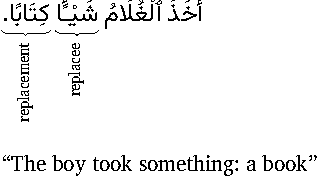
\includegraphics{A-Learners-Grammar-of-Classical-Standard-Arabic_files/figure-latex/unnamed-chunk-14-1.pdf}

In the above sentence, the word \foreignlanguage{arabic}{کِتَابًا} \enquote{a book} is the replacement of
\foreignlanguage{arabic}{شَيْـًٔا} \enquote{something}. Therefore, it is put in the same a-state.

The replacement is frequently used with proper nouns. For example,

\foreignlanguage{arabic}{ذَهَبَ ٱلْغُلَامُ إِلَىٰ بَيْتِ عَمِّهِ عَلِيٍّ.}\\
\enquote{The boy went to his uncle Ɛalī's house.}

In this sentence, the name \foreignlanguage{arabic}{عَلِيّ} Ɛalī is the replacement of the replacee \foreignlanguage{arabic}{عَمّ} \enquote{uncle}. Note, again, that the replacement comes after the replacee and matches it in state. However, the replacement does not need to come directly after the replacee. We can see that there is the pronoun \foreignlanguage{arabic}{ه} \enquote{his} between them.

Here is another example:

\foreignlanguage{arabic}{سَأَلَ ٱلطَّالِبُ مُعَاذٌ ٱلْمُعَلِّمَ سَعْدًا.}\\
\enquote{The student Muɛād͡h asked the teacher Saɛd.}

\section{Annexed names}\label{annexed-names}

So far we have only dealt with proper nouns that are single words. There are some proper nouns that may be formed from two words that are in an annexation. These belong to different categories:

\subsection{\texorpdfstring{\enquote{Slave of} names}{``Slave of'' names}}\label{slave-of-names}

Some names are formed by annexing the noun \foreignlanguage{arabic}{عَبْد} \emph{ɛabd} \enquote{a slave} to one of the names of Allāh. The most common of these names are:

\begin{itemize}
\tightlist
\item
  \foreignlanguage{arabic}{عَبْد ٱللَّـٰه} Ɛabd Allāh \enquote{the Slave of Allāh}
\item
  \foreignlanguage{arabic}{عَبْد ٱلرَّحْمَـٰن} Ɛabd al-Raḥmān \enquote{the Slave of the Most Merciful}
\end{itemize}

As usual, the base noun shall always be in the i-state. And the state of the annexe noun \foreignlanguage{arabic}{عَبْد} is variable, depending on it's function in the sentence. Example:

\foreignlanguage{arabic}{عَبْدُ ٱللَّـٰهِ هُوَ أَخُو عَبْدِ ٱلرَّحْمَـٰنِ.}
\enquote{Ɛabd Allāh is the brother of Ɛabd al-Raḥmān.}

\subsection{\texorpdfstring{\enquote{Parent of} names}{``Parent of'' names}}\label{parent-of-names}

It is common to call a man, not by his own given name, but rather by calling him the father of one of his children, usually his first born son. For example, if a man named \foreignlanguage{arabic}{أَحْمَد} \enquote{Aḥmad} had a son named \foreignlanguage{arabic}{زَيْد} \enquote{Zayd}, he may be called \foreignlanguage{arabic}{أَبُو زَيْد} Abū Zayd \enquote{Zayd's father}. Example of usage in a sentence:

\foreignlanguage{arabic}{ذَهَبْتُ إِلَىٰ بَيْتِ أَبِي زَيْدٍ.}\\
\enquote{I went to Abū Zayd's house.}\\
(Note how \foreignlanguage{arabic}{زَيْدٍ} has a nūnated \emph{i}-mark \foreignlanguage{arabic}{◌ٍ} in the i-state because it is fully-flexible.)

While using the name of first-born son is more common, a daughter's name could be used as well. Example,

\foreignlanguage{arabic}{سَأَلْتُ أَبَا رُقَيَّةَ سُؤالًا.}\\
\enquote{I asked Abū Ruqayyah a question.}\\
(Note how \foreignlanguage{arabic}{رُقَيَّةَ} has an \emph{a}-mark \foreignlanguage{arabic}{◌َ} in the i-state because it is semi-flexible.)

Women, too, are similarly called as the mother of one of their children. For example,
the wife of the Prophet
(may Allāh grant peace and confer blessing upon him)
\textsuperscript{2}\foreignlanguage{arabic}{أُمّ حَبِيبَة} Umm Ḥabībah
was called thus because she had a daughter named
\textsuperscript{2}\foreignlanguage{arabic}{حَبِيبَة}
from a previous marriage.

By the way, a person need not literally be a father or a mother to be called in such a way. These names may be applied as nicknames.

For example, the Companion of the Prophet
(may Allāh grant peace and confer blessing upon him)
was called
\textsuperscript{2}\foreignlanguage{arabic}{أَبُو هُرَيرَة}
Abū Hurayrah
because it is reported that he used to have a pet kitten (\foreignlanguage{arabic}{هُرَيْرَة}). Here is an example of this name in a sentence.

\foreignlanguage{arabic}{أَبُو هُرَيْرَةَ صَحَابِيٌّ جَلِيلٌ.}\\
\enquote{Abū Hurayrah is a great Companion.}\\
(Note how \foreignlanguage{arabic}{هُرَيْرَةَ} is now considered a semi-flexible proper noun even though it may originally have been derived from the common noun \enquote{a kitten}.)

Similarly, the Companion \foreignlanguage{arabic}{أَبُو بَکْرٍ} Abū Bakr is not known to have a son named \foreignlanguage{arabic}{بَکْر}.

It is often the case that a \enquote{parent of} name overtakes the actual given name of person in popularity, and becomes the person's name for all intents and purposes. Such is indeed the case for the Companions
\foreignlanguage{arabic}{أَبُو بَکْرٍ} Abū Bakr
and
\textsuperscript{2}\foreignlanguage{arabic}{أَبُو هُرَيرَة}
Abū Hurayrah.

\subsection{\texorpdfstring{\enquote{Son of} names}{``Son of'' names}}\label{son-of-names}

In a manner similar to \enquote{parent of} names, a person may be referred to as the son of his parent. For example, the Companion \textsuperscript{2}\foreignlanguage{arabic}{عُمَر} Ɛumar had a son named
\foreignlanguage{arabic}{عَبْد ٱللَّـٰه} Ɛabd Allāh. He is commonly known as \textsuperscript{2}\foreignlanguage{arabic}{ٱِبْن عُمَر} Ibn Ɛumar \enquote{Ɛumar's son}.

Attributing a son to his father is most common. But attributing him to a mother or other ancestor is also possible.

Examples:

\begin{itemize}
\tightlist
\item
  the Companion \foreignlanguage{arabic}{عَمَّار} was affectionately called \textsuperscript{2}\foreignlanguage{arabic}{ٱِبْن سُمَيَّة} Ibn Sumayyah \enquote{Sumayyah's son} by the Prophet
  (may Allāh grant peace and confer blessing upon him). His mother Sumayyah was an early martyr in Islām.
\item
  the famous scholar \foreignlanguage{arabic}{ٱِبْن کَثِير} Ibn Kat͡hīr is referred to by his grandfather's name \foreignlanguage{arabic}{کَثِير} Kat͡hīr.
\item
  a human being is called \textsuperscript{2}\foreignlanguage{arabic}{ٱِبْن آدَم} based on his being a descendent of the first man, the Prophet Adam.
\end{itemize}

\subsubsection{Full names}\label{full-names}

The full name of a person is formed by putting his given name first, and then his \enquote{son of} name after it as a replacement. Here is an example of a full name:

\foreignlanguage{arabic}{زَيْدُ بْنُ عَلِيٍّ}\\
Zayd the son of Ɛalī

Note some peculiarities of the full name:

\begin{itemize}
\tightlist
\item
  The name \foreignlanguage{arabic}{زَيْد} \enquote{Zayd} has lost its nūnation.
\item
  The word \foreignlanguage{arabic}{بْن} \enquote{son} is not written with its initial connecting hamzah \foreignlanguage{arabic}{ٱ}.
\end{itemize}

These peculiarities are only when forming a full name in this manner. Consider for example the following sentence:

\foreignlanguage{arabic}{زَيْدٌ ٱبْنُ عَلِيٍّ.}\\
\enquote{Zayd is the son of Ɛalī.}

In the above example, the name \foreignlanguage{arabic}{زَيْدٌ} is nūnated and \foreignlanguage{arabic}{ٱبْن} is written with its connecting hamzah \foreignlanguage{arabic}{ٱ}. Therefore this is not an expression of the full name in a replacee-replacement format. Rather, \foreignlanguage{arabic}{ٱبْنُ أَحْمَدَ} here is the information of the sentence.

For women, the word \foreignlanguage{arabic}{بِنْت} is used instead of \foreignlanguage{arabic}{بْن}.

Example:

\foreignlanguage{arabic}{قَرَأَتِ ٱلْمُعَلِّمَةُ کِتَابَ ٱلطَّالِبَةِ زَيْنَبَ بِنْتِ أَحْمَدَ.}\\
\enquote{The teacher read the book of the student Zaynab the daughter of Aḥmad.}

The names of multiple forefathers may be strung together in this way separated by \foreignlanguage{arabic}{بْن}. For example:

\foreignlanguage{arabic}{ٱِسْمُ نَبِيِّنَا مُحَمَّدُ بْنُ عَبْدِ ٱللَّـٰهِ بْنِ عَبْدِ ٱلْمُطَّلِبِ.}\\
\enquote{Our prophet's name is Muḥammad the son of Ɛabd Allāh the son of Ɛabd al-Muṭṭalib.}\\
(Note that the second \foreignlanguage{arabic}{بْنِ} is in the i-state to match the state of the annexe noun \foreignlanguage{arabic}{عَبْدِ} in \foreignlanguage{arabic}{عَبْدِ ٱللّـٰه}.)

We will deal with complete full names in section~\ref{complete-full-names} below.

\subsection{Other annexed names}\label{other-annexed-names}

Other words besides
\foreignlanguage{arabic}{عَبْد},
\foreignlanguage{arabic}{أَب},
\foreignlanguage{arabic}{أُمّ},
and
\foreignlanguage{arabic}{ٱِبْن}
may be used in annexed names too. Here are some examples:

\begin{itemize}
\item
  \foreignlanguage{arabic}{ذُو ٱلْقَرْنَينِ} D͡hu l-Qarnayn \enquote{He of the two horns}
\item
  \foreignlanguage{arabic}{مَدِينَة ٱلنَّبِي} \emph{madinatu -nnabiyyi} \enquote{The City of the Prophet}, frequently reduced to simply \foreignlanguage{arabic}{ٱَلْمَدِينَة} \enquote{al-Madīnah}.

  Context is used to infer whether by \foreignlanguage{arabic}{ٱَلْمَدِينَة} is meant \enquote{al-Madīnah} or \enquote{the city}.
\item
  \foreignlanguage{arabic}{ٱمْرُؤُ ٱلْقَيْس} Imruʾ al-Qays \enquote{The man of al-Qays}, a pre-Islāmic poet.
\end{itemize}

\section{\texorpdfstring{Names beginning with \foreignlanguage{arabic}{ٱَلْ}}{Names beginning with ٱَلْ}}\label{names-beginning-with-ux671ux644}

Most names do not begin with \foreignlanguage{arabic}{ٱَلْ}. Some, however, do begin with \foreignlanguage{arabic}{ٱَلْ}. Examples:

\begin{longtable}[]{@{}
  >{\raggedleft\arraybackslash}p{(\columnwidth - 6\tabcolsep) * \real{0.2143}}
  >{\raggedright\arraybackslash}p{(\columnwidth - 6\tabcolsep) * \real{0.2857}}
  >{\raggedleft\arraybackslash}p{(\columnwidth - 6\tabcolsep) * \real{0.2143}}
  >{\raggedright\arraybackslash}p{(\columnwidth - 6\tabcolsep) * \real{0.2857}}@{}}
\toprule\noalign{}
\endhead
\bottomrule\noalign{}
\endlastfoot
\foreignlanguage{arabic}{ٱَلْحَسَن} & al-Ḥasan & \foreignlanguage{arabic}{ٱَلزُّبَيْر} & al-Zubayr \\
\foreignlanguage{arabic}{ٱَلْحُسَيْن} & al-Ḥusayn & \foreignlanguage{arabic}{ٱَلنُّعْمَان} & al-Nuɛmān \\
\foreignlanguage{arabic}{ٱَلْعَبَّاس} & al-Ɛabbās & \foreignlanguage{arabic}{ٱَلْحَارِث} & al-Ḥārit͡h \\
\end{longtable}

If a proper noun begins with \foreignlanguage{arabic}{ٱَلْ} then the question of its flexibility is mostly irrelevant.
This is because noun beginning with with \foreignlanguage{arabic}{ٱَلْ} display their state fully, regardless of whether or not they are semi-flexible without the \foreignlanguage{arabic}{ٱَلْ}. Examples:

\foreignlanguage{arabic}{ٱَلْحَسَنُ حَفِيدُ رَسُولِ ٱللَّـٰهِ صلى اللّه عليه وسلم.}\\
\enquote{al-Ḥasan is the grandson of the messenger of Allāh (may Allāh grant peace and confer blessing upon him).}\\
(u-state displayed with \foreignlanguage{arabic}{◌ُ}.)

\foreignlanguage{arabic}{سَأَلَ ٱلرَّجُلُ ٱلنُّعْمَانَ عَنْ أَمْرٍ.}\\
\enquote{The man asked al-Nuɛmān about a matter.}\\
(a-state displayed with \foreignlanguage{arabic}{◌َ}.)

\foreignlanguage{arabic}{ذَهَبْتُ إِلَى بَيْتِ ٱلنُّعْمَانِ.}\\
\enquote{I went to al-Nuɛmān's house.}\\
(i-state displayed with \foreignlanguage{arabic}{◌ِ}.)

Names that begin with \foreignlanguage{arabic}{ٱَلْ} can sometimes lose their initial \foreignlanguage{arabic}{ٱَلْ}. Sometimes, this is systematic, as we will lear in section~\ref{calling-names-with-al}.
Other times, it's hard to tell why.

Conversely, names that don't begin with \foreignlanguage{arabic}{ٱَلْ} can sometimes gain it.

Examples:

\begin{itemize}
\item
  The name of the daughter of the Companion \foreignlanguage{arabic}{أَبُو ٱلدَّرْدَاء} Abu l-Dardāʾ is actually \textsuperscript{2}\foreignlanguage{arabic}{دَرْدَاء} Dardāʾ, not \foreignlanguage{arabic}{ٱَلدَّرْدَاء}.
\item
  The son of the uncle of the Prophet
  (may Allāh grant peace and confer blessing upon him)
  \foreignlanguage{arabic}{ٱَلْعَبَّاس} al-Ɛabbās
  is called
  \foreignlanguage{arabic}{ٱِبْن عَبَّاس} Ibn ɛabbās, not \foreignlanguage{arabic}{ٱِبْن ٱلْعَبَّاس}.
\end{itemize}

However, the son of
\foreignlanguage{arabic}{ٱَلْزُّبَيْر} al-Zubayr\textbar{}
is called
\foreignlanguage{arabic}{ٱِبْن ٱلْزُّبَيْر} Ibn al-Zubayr with the \foreignlanguage{arabic}{ٱَلْ}.

\section{Place names}\label{place-names}

Place names are generally feminine. Because of their feminine gender, those not beginning with \foreignlanguage{arabic}{ٱَلْ} will be semi-flexible according to section~\ref{feminine-names} above.

Examples of place names are:

\begin{longtable}[]{@{}
  >{\raggedleft\arraybackslash}p{(\columnwidth - 6\tabcolsep) * \real{0.2143}}
  >{\raggedright\arraybackslash}p{(\columnwidth - 6\tabcolsep) * \real{0.2857}}
  >{\raggedleft\arraybackslash}p{(\columnwidth - 6\tabcolsep) * \real{0.2143}}
  >{\raggedright\arraybackslash}p{(\columnwidth - 6\tabcolsep) * \real{0.2857}}@{}}
\toprule\noalign{}
\endhead
\bottomrule\noalign{}
\endlastfoot
\textsuperscript{2}\foreignlanguage{arabic}{مَکَّة} & Makkah & \foreignlanguage{arabic}{ٱَلْمَدِينَة} & al-Madīnah \\
\textsuperscript{2}\foreignlanguage{arabic}{دِمَشْق} & Damascus & \foreignlanguage{arabic}{ٱَلْقَاهِرَة} & Cairo \\
\textsuperscript{2}\foreignlanguage{arabic}{بَغْدَاد} & Bag͡hdād & \foreignlanguage{arabic}{ٱَلْهِنْد} & India \\
\textsuperscript{2}\foreignlanguage{arabic}{مِصْر} & Egypt & \foreignlanguage{arabic}{ٱَلصِّين} & China \\
\textsuperscript{2}\foreignlanguage{arabic}{فَارِس} & Persia & \foreignlanguage{arabic}{ٱَلرُّوم} & Rome \\
\textsuperscript{2}\foreignlanguage{arabic}{تَبُوک} & Tabūk & \foreignlanguage{arabic}{ٱَلْبَصْرَة} & Baṣrah \\
\end{longtable}

Example of use:

\foreignlanguage{arabic}{ذَهَبَ ٱلرَّجُلُ إِلَىٰ مَکَّةَ ٱلْمُکَرَّمَةِ وَٱلْمَدِينَةِ ٱلْمُنَوَّرَةِ.}\\
\enquote{The man went to the ennobled Makkah and the illuminated al-Madīnah.}

While most place names are feminine, a few are masculine. Among these are:

\begin{longtable}[]{@{}rlrl@{}}
\toprule\noalign{}
\endhead
\bottomrule\noalign{}
\endlastfoot
\foreignlanguage{arabic}{ٱَلْيَمَن} & Yemen & \foreignlanguage{arabic}{ٱَلشَّام} & the Levant \\
\foreignlanguage{arabic}{ٱَلْعِرَاق} & Iraq & & \\
\end{longtable}

\section{Names of tribes}\label{names-of-tribes}

Here are examples of names of tribes:

\begin{longtable}[]{@{}
  >{\raggedleft\arraybackslash}p{(\columnwidth - 6\tabcolsep) * \real{0.2143}}
  >{\raggedright\arraybackslash}p{(\columnwidth - 6\tabcolsep) * \real{0.2857}}
  >{\raggedleft\arraybackslash}p{(\columnwidth - 6\tabcolsep) * \real{0.2143}}
  >{\raggedright\arraybackslash}p{(\columnwidth - 6\tabcolsep) * \real{0.2857}}@{}}
\toprule\noalign{}
\endhead
\bottomrule\noalign{}
\endlastfoot
\foreignlanguage{arabic}{قُرَيش} & Qurays͡h & \foreignlanguage{arabic}{ٱَلْأَوْس} & al-Aws \\
\foreignlanguage{arabic}{بَنُو تَمِيم} & Banū Tamīm & \foreignlanguage{arabic}{ٱَلْخَزْرَج} & al-K͡hazraj \\
\textsuperscript{2}\foreignlanguage{arabic}{هَوَازِن} & Hawāzin & \textsuperscript{2}\foreignlanguage{arabic}{بَنُو إِسْرَائِيل} & Banū Isrāʾīl \\
\end{longtable}

Tribes are usually called by the name of their progenitor. For example, \textsuperscript{2}\foreignlanguage{arabic}{إِسْرَائِيل} Isrāʾīl is a name of the Prophet \textsuperscript{2}\foreignlanguage{arabic}{يَعْقُوب} Yaɛqūb.
The \emph{ūn} sound plural \foreignlanguage{arabic}{بَنُونَ} \enquote{sons/children} is annexed to the name
\textsuperscript{2}\foreignlanguage{arabic}{إِسْرَائِيل} Isrāʾīl
to get the name of the tribe
\textsuperscript{2}\foreignlanguage{arabic}{بَنُو إِسْرَائِيل} Banū Isrāʾīl \enquote{the children of Isrāʾīl}. In the a- and i-states, this becomes
\textsuperscript{2}\foreignlanguage{arabic}{بَنِي إِسْرَائِيل} Banī Isrāʾīl.

Not all tribe names have \foreignlanguage{arabic}{بَنُونَ} \enquote{sons} annexed to them, but many do. And often it is optional to keep or drop the annexed \foreignlanguage{arabic}{بَنُونَ}. Examples:

\begin{itemize}
\tightlist
\item
  \foreignlanguage{arabic}{قُرَيْش} Qurays͡h usually does not have \foreignlanguage{arabic}{بَنُونَ} annexed to it.
\item
  \foreignlanguage{arabic}{بَنُو تَمِيم} Banū Tamīm may optionally drop the annexed \foreignlanguage{arabic}{بَنُونَ} and be called simply \foreignlanguage{arabic}{تَمِيم} Tamīm.
\end{itemize}

\subsection{Flexibility of tribe names}\label{flexibility-of-tribe-names}

The flexibility of tribe names depends on the name. Here are some examples:

\begin{itemize}
\item
  \textsuperscript{2}\foreignlanguage{arabic}{إِسْرَائِيل} Isrāʾīl is a name of foreign origin and is therefore semi-flexible. Example:

  \foreignlanguage{arabic}{بَعَثَ ٱللَّـٰهُ مُوسَىٰ إِلَىٰ بَنِي إِسْرَائِيلَ.}\\
  \enquote{Allāh sent Mūsā to the children of Isrāʾīl.}
\item
  \foreignlanguage{arabic}{قُرَيْش} Qurays͡h and \foreignlanguage{arabic}{تَمِيم} Tamīm are native Arabic masculine names and are therefore fully-flexible. Example:

  \foreignlanguage{arabic}{قُرَيشٌ وَبَنُو تَمِيمٍ قَبِيلَتَانِ.}\\
  \enquote{Qurays͡h and Banū Tamīm are tribes\textsubscript{2}.}
\item
  \textsuperscript{2}\foreignlanguage{arabic}{هَوَازِن} Hawāzin is on the semi-flexible noun pattern \textsuperscript{2}\foreignlanguage{arabic}{فَفَافِف} and is therefore semi-flexible.
\end{itemize}

\subsection{Gender of tribe names}\label{gender-of-tribe-names}

Tribe names are unusual in that they are treated as both singular feminine and plural masculine.
If the tribe name is the doer of a verb then it is usually treated as singular feminine.
Otherwise, for example, if it comes before the verb, then the plural masculine pronouns are used for it.

Example:

\foreignlanguage{arabic}{سَکَنَتْ قُرَيْشٌ مَکَّةَ وَعَبَدُوا ٱلْأَصْنَامَ.}\\
\enquote{Qurays͡h dwelled in Makkah and they worshipped idols.}

\section{Titles}\label{titles}

Titles are common nouns that denote a rank or position of a person. Titles in English include: Doctor, Mister, and King. For example:

\begin{itemize}
\tightlist
\item
  King David
\item
  Mr.~Smith
\item
  Dr.~Adams
\end{itemize}

Here are some examples of titles in Arabic:

\begin{longtable}[]{@{}rlrl@{}}
\toprule\noalign{}
\endhead
\bottomrule\noalign{}
\endlastfoot
\foreignlanguage{arabic}{ٱَلنَّبِيّ} & Prophet & \foreignlanguage{arabic}{ٱَلْإِمَام} & Imām \\
\foreignlanguage{arabic}{ٱَلْمَلِک} & King & \foreignlanguage{arabic}{ٱَلشَّيْخ} & S͡hayk͡h \\
\foreignlanguage{arabic}{ٱَلْأَمِير} & Commander & \foreignlanguage{arabic}{ٱَلْحَافِظ} & Ḥāfiḍ͡h \\
\foreignlanguage{arabic}{ٱَلْقَاضِي} & Judge & \foreignlanguage{arabic}{ٱَلْأُسْتَاذ} & Professor \\
\end{longtable}

Some Arabic titles are left untranslated in English like

\begin{itemize}
\tightlist
\item
  \foreignlanguage{arabic}{ٱَلْإِمَام} Imām (a leader)
\item
  \foreignlanguage{arabic}{ٱَلشَّيْخ} S͡hayk͡h (a venerable man)
\item
  \foreignlanguage{arabic}{ٱَلْحَافِظ} Ḥāfiḍ͡h (one who has memorized, and preserved religious texts)
\end{itemize}

\subsection{Titles as replacees}\label{titles-as-replacees}

Titles are usually placed in front a proper noun and made definite with \foreignlanguage{arabic}{ٱَلْ} to match the proper noun. For example,

\foreignlanguage{arabic}{سَأَلَ رَجُلٌ ٱلْإِمَامَ مَالِکًا عَنْ أَمْرٍ.}\\
\enquote{A man asked Imām Mālik about a matter.}

In the above sentence, the title \foreignlanguage{arabic}{ٱَلْإِمَامَ} Imām is a replacee and the name \foreignlanguage{arabic}{مَالِکًا} Mālik is the replacement.

Some titles are formed from annexations. Examples:

\begin{longtable}[]{@{}
  >{\raggedleft\arraybackslash}p{(\columnwidth - 6\tabcolsep) * \real{0.2143}}
  >{\raggedright\arraybackslash}p{(\columnwidth - 6\tabcolsep) * \real{0.2857}}
  >{\raggedleft\arraybackslash}p{(\columnwidth - 6\tabcolsep) * \real{0.2143}}
  >{\raggedright\arraybackslash}p{(\columnwidth - 6\tabcolsep) * \real{0.2857}}@{}}
\toprule\noalign{}
\endhead
\bottomrule\noalign{}
\endlastfoot
\foreignlanguage{arabic}{خَلِيفَةُ رَسُولِ ٱللَّـٰهِ} & the Successor of the Messenger of Allāh & \foreignlanguage{arabic}{سَيْفُ ٱللَّـٰهِ} & the Sword of Allāh \\
\foreignlanguage{arabic}{أَمِيرُ ٱلْمُؤْمِنِينَ} & the Commander of the Believers & \foreignlanguage{arabic}{عِمَادُ ٱلدِّينِ} & the Pillar of the Faith \\
\foreignlanguage{arabic}{أُمُّ ٱلْمُؤْمِنِينَ} & the Mother of the Believers & \foreignlanguage{arabic}{صَلَاحُ ٱلدِّينِ} & the Righteousness of the Faith \\
\end{longtable}

Example:

\foreignlanguage{arabic}{أُمُّ ٱلْمُؤْمِنِينَ عَائِشَةُ هِيَ ٱِبْنَةُ خَلِيفَةِ رَسُولِ ٱللَّـٰهِ أَبِي بَکْرٍ.}\\
\enquote{The Mother of the Believers Ɛāʾis͡hah is the daughter of the Successor of the Messenger of Allāh Abū Bakr.}

\subsection{Titles in annexations}\label{titles-in-annexations}

Some prominent inanimate objects, like mountains, rivers, and cities, may have titles. For example:

\begin{itemize}
\tightlist
\item
  Mount Everest
\item
  the river Nile
\item
  the city of Damascus
\end{itemize}

In Arabic, the titles for these objects usually don't occur as replacees as they do for persons. Rather, the title is annexed to the proper noun in an annexation. Examples:

\begin{longtable}[]{@{}
  >{\raggedleft\arraybackslash}p{(\columnwidth - 6\tabcolsep) * \real{0.2143}}
  >{\raggedright\arraybackslash}p{(\columnwidth - 6\tabcolsep) * \real{0.2857}}
  >{\raggedleft\arraybackslash}p{(\columnwidth - 6\tabcolsep) * \real{0.2143}}
  >{\raggedright\arraybackslash}p{(\columnwidth - 6\tabcolsep) * \real{0.2857}}@{}}
\toprule\noalign{}
\endhead
\bottomrule\noalign{}
\endlastfoot
\foreignlanguage{arabic}{جَبَلُ أُحُدٍ} & Mount Uḥud & \foreignlanguage{arabic}{مَدِينَةُ دِمَشْقَ} & the city of Damascus \\
\foreignlanguage{arabic}{نَهْرُ ٱلنِّيلِ} & the river Nile & \foreignlanguage{arabic}{شَهْرُ رَمَضَانَ} & the month of Ramaḍān \\
\foreignlanguage{arabic}{يَوْمُ ٱلْجُمُعَةِ} & the day of Friday & \foreignlanguage{arabic}{سُورَةُ ٱلْفَاتِحَةِ} & the Sūrah of al-Fātiḥah \\
\end{longtable}

Example:

\foreignlanguage{arabic}{قَرَأَتِ ٱلْجَارِيَةُ سُورَةَ ٱلْفَاتِحَةِ فِي شَهْرِ رَمَضَانَ.}\\
\enquote{The girl read the Sūrah of al-Fātiḥah in the month of Ramaḍān.}

\section{Nicknames}\label{nicknames}

Nicknames are often given to people. They are usually descriptive of some physical quality or character trait of the person. For example, the Companion Abū Bakr was given the nickname \foreignlanguage{arabic}{ٱلصِّدِّيق} \enquote{the steadfast affirmer of the truth}.

Nicknames usually come after a person's name as a replacement.

\foreignlanguage{arabic}{أَبُو بَکَرٍ ٱلصِّدِّيقُ هُوَ خَلِيفَةُ رَسُولِ ٱللَّـٰهِ.}\\
\enquote{Abū Bakr the steadfast affirmer of the truth is the successor of the messenger of Allāh.}

\foreignlanguage{arabic}{قَرَأَ سُلَيْمَانُ ٱلأَعْمَشُ ٱلْقُرْآنَ.}\\
\enquote{Sulaymān the weak-sighted read the Qurʾān.}

\section{The affiliate adjectival noun}\label{the-affiliate-adjectival-noun}

The affiliate adjectival noun is a kind of adjectival noun that indicates an affiliation.

Here are some examples of affiliate adjectival nouns:

\begin{longtable}[]{@{}
  >{\raggedleft\arraybackslash}p{(\columnwidth - 6\tabcolsep) * \real{0.2143}}
  >{\raggedright\arraybackslash}p{(\columnwidth - 6\tabcolsep) * \real{0.2857}}
  >{\raggedleft\arraybackslash}p{(\columnwidth - 6\tabcolsep) * \real{0.2143}}
  >{\raggedright\arraybackslash}p{(\columnwidth - 6\tabcolsep) * \real{0.2857}}@{}}
\toprule\noalign{}
\endhead
\bottomrule\noalign{}
\endlastfoot
\foreignlanguage{arabic}{عِرَاقِيّ} & an Iraqi & \foreignlanguage{arabic}{قُرَشِيّ} & a Qurays͡hite \\
\foreignlanguage{arabic}{مَکِّي} & a Makkan & \foreignlanguage{arabic}{تَمِيمِيّ} & a Tamīmian \\
\foreignlanguage{arabic}{دِمَشْقِيّ} & a Damascan & \foreignlanguage{arabic}{إِسْرَائِيلِيّ} & an Isrāʾīlite \\
\foreignlanguage{arabic}{شَافِعِيّ} & a S͡hāfiɛite & \foreignlanguage{arabic}{حَنَفِيّ} & a Ḥanafī \\
\foreignlanguage{arabic}{مَالِکِيّ} & a Mālikī & \foreignlanguage{arabic}{حَنْبَلِيّ} & a Ḥanbalī \\
\end{longtable}

Note the following about affiliate adjectival nouns:

\begin{itemize}
\tightlist
\item
  Generally, the ending \foreignlanguage{arabic}{◌ِيّ} \emph{-iyy} is suffixed to a noun to create an affiliate adjectival noun.
\item
  The \foreignlanguage{arabic}{ة} ending is removed before adding the \foreignlanguage{arabic}{◌ِيّ} \emph{-iyy} suffix.
\item
  Sometimes there are other internal changes to the word before this suffix is added. For example,

  \begin{itemize}
  \tightlist
  \item
    \foreignlanguage{arabic}{قُرَيْش} becomes \foreignlanguage{arabic}{قُرَشِيّ}
  \end{itemize}
\item
  The affiliate adjectival noun may be formed from any of the names of a person. (Usually, one of the more distinctive names is chosen.) For example:

  \begin{itemize}
  \tightlist
  \item
    A follower of the school of thought of \foreignlanguage{arabic}{ٱَلْإِمَام أَبُو حَنِيفَة} Imām Abū Ḥanīfah is called \foreignlanguage{arabic}{حَنَفِيّ} \enquote{a Ḥanafī}.
  \item
    A follower of the school of thought of \foreignlanguage{arabic}{ٱَلْإِمَام أَحْمَد بْن حَنْبَل} Imām Aḥmad ibn Ḥanbal is called \foreignlanguage{arabic}{حَنْبَلِيّ} \enquote{a Ḥanbalī}.
  \end{itemize}
\end{itemize}

We will treat adjectival nouns more fully in chapter~\ref{the-affiliate-adjective-chapter}.

Afflilate adjectival nouns frequently occur with proper nouns. They come after the proper noun as a replacement, and are made definite by \foreignlanguage{arabic}{ٱَلْ} to match the proper noun in definiteness. Examples:

\foreignlanguage{arabic}{ٱِبْن کَثِيرٍ ٱلدِّمَشْقِيُّ مُفَسِّرٌ وَمُؤَرِّخٌ.}\\
\enquote{Ibn Kat͡hīr the Damascan is an exegete and a historian.}

\section{Complete full names}\label{complete-full-names}

We have already studied how a basic full name is formed in section~\ref{full-names}. Here, we will expand on that topic.

The complete full name of a person is formed by placing some or all of his different names in a particular order. Each name in the order is a replacement of one of the names before it. Generally, the order is:

\begin{enumerate}
\def\labelenumi{\roman{enumi}.}
\tightlist
\item
  Titles
\item
  \enquote{Father of} name
\item
  Given name
\item
  \enquote{Son of} names
\item
  Affiliate names
\end{enumerate}

The nickname's position is variable.

Here are some examples of full names in varying degrees of completeness:

\foreignlanguage{arabic}{عَائِشَةُ هِيَ ٱبْنَةُ خَلِيفَةِ رَسُولِ ٱللَّـٰهِ أَبِي بَکْرٍ ٱلصِّدِّيقِ.}\\
\enquote{Ɛāʾis͡hah is the daughter of the Successor of the Messenger of Allāh, Abū Bakr, the steadfast affirmer of the truth.}

\foreignlanguage{arabic}{قَتَلَ أَبُو لُؤْلُؤَةَ ٱلْمَجُوسِيُّ أَمِيرَ ٱلْمُؤْمِنِينَ أَبَا حَفْصٍ عُمَرَ بْنَ ٱلْخَطَّابِ.}\\
\enquote{Abū Luʾluʾah, the Magian killed the Commander of the Believers, Abū Ḥafṣ, Ɛumar the son of al-K͡haṭṭāb.}

\foreignlanguage{arabic}{ٱلْحَافِظُ ٱلْمُؤَرِّخُ ٱلْمُفَسِّرُ عِمَادُ ٱلدِّينِ أَبُو ٱلْفِدَاءِ إِسْمَاعِيلُ بْنُ عُمَرَ بْنِ کَثِيرٍ ٱلْقُرَشِيُّ ٱلدِّمَشْقِيُّ ٱلشَّافِعِيُّ}\\
\enquote{The Ḥāfiḍ͡h, the historian, the exegete, the Pillar of the Faith, the father of al-Fidāʾ, Ismāʾīl the son of Ɛumar the son of Kat͡hīr, the Qurays͡hite, the Damascan, the S͡hāfiɛite}\\
(Note how the second \foreignlanguage{arabic}{بْنِ} is in the i-state because it is a replacement of \foreignlanguage{arabic}{عُمَرَ} which is in the i-state because it is a base noun of the first \foreignlanguage{arabic}{بْنُ}.)

\chapter{Calling out}\label{calling-out}

\section{Introduction}\label{introduction-13}

When calling out to someone in Arabic, the particle \foreignlanguage{arabic}{يَا} \emph{yā} is usually prefixed to the person's name. For example,

\foreignlanguage{arabic}{ٱَلسَّلَامُ عَلَيْکُمْ يَا زَيْنَبُ.}\\
\emph{ʾassalāmu ɛalaykum yā zaynabu.}\\
\enquote{Peace be upon you, O Zaynab.}

There are different rules regarding the state markings of the noun following \foreignlanguage{arabic}{يَا} \emph{yā} and we will describe them in the following sections.

\section{Calling out to specific persons}\label{calling-out-to-specific-persons}

\subsection{Using single word personal names}\label{using-single-word-personal-names}

When a specific person is called out to, and the name used to call him consists of a single word, then that word shall be in the u-state. The sentence above is an example of this rule where the name \foreignlanguage{arabic}{زَينَبُ} \emph{zaynabu} \enquote{Zaynab} is in the u-state.

If the word would be nūnated, then the nūnation is dropped. So, for example, the name \foreignlanguage{arabic}{زَيْدٌ} \emph{zaydun} \enquote{Zayd} usually is nūnated. But when used for being called out to, the nūnation is dropped and it becomes:

\foreignlanguage{arabic}{ٱَلسَّلَامُ عَلَيْکُمْ يَا زَيْدُ.}\\
\emph{ʾassalāmu ɛalaykum yā zaydu.}\\
\enquote{Peace be upon you, O Zayd.}

\subsection{Using single word indefinite common nouns}\label{using-single-word-indefinite-common-nouns}

The examples above show the person being called out to using a personal name. Instead of a personal name, a common noun can also be used with the same rule. Examples:

\foreignlanguage{arabic}{ٱَلسَّلَامُ عَلَيْکُمْ يَا غُلَامُ.}\\
\emph{ʾassalāmu ɛalaykum yā g͡hulāmu.}\\
\enquote{Peace be upon you, O you boy.}

\foreignlanguage{arabic}{ٱَلسَّلَامُ عَلَيْکُمْ يَا جَارِيَةُ.}\\
\emph{ʾassalāmu ɛalaykum yā jāriyatu.}\\
\enquote{Peace be upon you, O you girl.}

In English, we have shown that a specific person is being called using the word \enquote{you}, e.g., \enquote{O you boy}. Duals and plurals are also allowed, again with the same rule:

\foreignlanguage{arabic}{يَا رِجَالُ، قَدْ حَدَثَ أَمْرٌ.}\\
\emph{yā rijālu qad ḥadat͡ha ʾamrun.}\\
\enquote{O you men, a matter has occurred.}

Note how the word \foreignlanguage{arabic}{رِجَالُ} \emph{rijālu} \enquote{men} is not nūnated because the word is used to call out to the specific persons.

Similarly,

\foreignlanguage{arabic}{يَا لَاعِبَانِ بَدَأْتُمَا ٱللَّعِبَ وَمَا فَعَلْتُمَا ٱلْعَمَلَ.}\\
\emph{yā lāɛibāni badaʾtuma -llaɛiba wamā faɛaltuma -lɛamal.}\\
\enquote{O you players\textsubscript{2}, you have started playing and you have not done the work.}

\subsection{Using single word definite common nouns}\label{using-single-word-definite-common-nouns}

When using a common noun to call out to a person, especially if the common noun is a title, it is often desired to make the common noun definite with \foreignlanguage{arabic}{ٱَلْ}. In this case, the particle \foreignlanguage{arabic}{يَا} \emph{yā} is modified to \foreignlanguage{arabic}{أَيُّهَا} \emph{ʾayyuhā}, or sometimes \foreignlanguage{arabic}{يَا أَيُّهَا} \emph{yā ʾayyuhā}. Examples:

\foreignlanguage{arabic}{يَا أَيُّهَا ٱلْأُسْتَاذُ، قَدْ فَعَلْتُ ٱلْوَاجِبَ.}\\
\emph{yā ʾayyuha -lʾustād͡hu, qad faɛaltu -lwājiba}\\
\enquote{O you the Professor, I have done the obligatory {[}work{]}.}

\foreignlanguage{arabic}{أَنَا سَقِيمٌ أَيُّهَا ٱلطَّبِيبُ.}\\
\emph{ʾana saqīmun, ʾayyuha -ṭṭabību.}\\
\enquote{I am ill, O you the Doctor.}

If the person being called out to is feminine, then \foreignlanguage{arabic}{أَيُّهَا} \emph{ʾayyuhā} is modified to \foreignlanguage{arabic}{أَيَّتُهَا} \emph{ʾayyatuhā}. For example:

\foreignlanguage{arabic}{أَيَّتُهَا ٱلْمُعَلِّمَةُ، هَـٰذَا کِتَابِي.}\\
\emph{ʾayyatuha -lmuɛallimatu, hād͡hā kitābi.}\\
\enquote{O you the teacher\textsubscript{f}, this is my book.}

\subsection{Using multiple words}\label{using-multiple-words}

The above discussion pertains to calling out to the addressed person with a single word. Often times a person's name may consist of multiple words. For example:

\begin{itemize}
\item
  \foreignlanguage{arabic}{عَبْدُ ٱللَّـٰهِ}\\
  \emph{ɛabdu -llāhi}\\
  \enquote{Ɛabd Allāh}
\item
  \foreignlanguage{arabic}{أَبُو بَکْرٍ}\\
  \emph{ʾabū bakrin}\\
  \enquote{Abū Bakr}
\item
  \foreignlanguage{arabic}{صَلَاحُ ٱلدِّينِ}\\
  \emph{ṣalāḥu -ddīni}\\
  \enquote{Salāḥ ad-Dīn}
\end{itemize}

In this case, then instead of the u-state, the word is put into the a-state. Furthermore, the nūnation, if any, is preserved. Examples:

\foreignlanguage{arabic}{مَا عَرَفْتُ ذَ ٰلِکَ ٱلرَّجُلَ، يَا عَبْدَ ٱللَّـٰهِ.}\\
\emph{mā ɛaraftu d͡hālika -rrajula, yā ɛabda -llāhi.}\\
\enquote{I have not recognized that man, O Ɛabd Allāh.}

\foreignlanguage{arabic}{يَا أَبَا بَکْرٍ، أَنْتَ رَجُلٌ کَرِيمٌ.}\\
\emph{yā ʾabā bakrin, ʾanta rajulun karīmun}\\
\enquote{O Abū Bakr, You are a noble man.}

\foreignlanguage{arabic}{يَا صَلَاحَ ٱلدِّينِ، صَبَرْتَ فَنَصَرَکَ ٱللَّـٰهُ.}\\
\emph{yā ṣalāḥa -ddīni, ṣabarta fanaṣaraka -llāhu.}\\
\enquote{O Salāḥ ad-Dīn, you were patient so Allāh gave you victory.}

If, instead of a personal name, a noun phrase consisting of multiple words is used to call out to a person, then in this case as well, the first noun shall be in the a-state. Examples:

\foreignlanguage{arabic}{يَا أَمِيرَ ٱلْمُؤمِنِينَ، قَدْ حَضَرَ ٱلْقَوْمُ.}\\
\emph{yā ʾamīra -lmuʾminīna, qad ḥaḍara -lqawmu.}\\
\enquote{O Commander of the Believers, the people are present.}

\foreignlanguage{arabic}{يَا ٱبْنَ أَخِي، قَدْ سَقَطَ قَلَمُکَ عَلَى ٱلْأَرْضِ.}\\
\emph{ya -bna ʾak͡hī, qad saqaṭa qalamuka.}\\
\enquote{O my nephew, your pen has fallen on the ground.}

\foreignlanguage{arabic}{يَا تَلَامِيذَ ٱلْمَدْرَسَةِ، ٱلْعِلْمُ أَمَانَةٌ.}\\
\emph{yā talāmīd͡ha -lmadrasati, -lɛilmu ʾamānatun.}\\
\enquote{O pupils of the school, knowledge is a trust.}

When multiple words are used to call out to a person, the second word in the noun-chain may be a pronoun. Here too, the first noun shall be in the a-state. Examples:

\foreignlanguage{arabic}{يَا أَبانا}\\
\emph{yā ʾabānā}\\
\enquote{O our father}

\section{Calling out to unspecified persons}\label{calling-out-to-unspecified-persons}

All the discussion so far has pertained to calling out to specific persons. So for example, when you say,

\foreignlanguage{arabic}{يَا مُسْلِمُ، نَصْرُ ٱللَّـٰهِ قَرِيبٌ.}\\
\emph{yā muslimu, naṣru -llāhi qarībun.}\\
\enquote{O you Muslim, the victory of Allāh is near.}

then you are addressing a specific Muslim, who is perhaps in front of you.

If an unspecified person or persons are being called out, then the word used to call out is put into the a-state. Furthermore, the nūnation, if any, is preserved. So if you want to address any unspecific Muslim, you will say:

\foreignlanguage{arabic}{يَا مُسْلِمًا، نَصْرُ ٱللَّـٰهِ قَرِيبٌ.}\\
\emph{yā musliman, naṣru -llāhi qarībun.}\\
\enquote{O {[}any{]} Muslim, the victory of Allāh is near.}

If multiple words are used, whether or not the person called out to is specific or unspecified, then too the first noun is put in the a-state.

\foreignlanguage{arabic}{يَا لَاعِبِي لُعَبٍ، ٱلْوَقْتُ ثَمِينٌ.}\\
\emph{yā lāɛibī luɛabini, -lwaqtu t͡hamīnun.}\\
\enquote{O {[}any{]} players of games, time is precious.}

\section{\texorpdfstring{Omitting \foreignlanguage{arabic}{يَا} \emph{yā}}{Omitting يَا yā}}\label{omitting-ux64aux627-ya}

When calling out to someone, it is permissible to omit the \foreignlanguage{arabic}{يَا} \emph{yā}, especially when the person being called is very near. So, instead of saying,

\foreignlanguage{arabic}{يَا زَيْدُ، سُؤالُکَ جَيِّدٌ.}\\
\emph{yā zaydu, suʾāluka jayyidun.}\\
\enquote{O Zayd, your question is excellent.}

it is permissible to say:

\foreignlanguage{arabic}{زَيْدُ، سُؤالُکَ جَيِّدٌ.}\\
\emph{zaydu, suʾāluka jayyidun.}\\
\enquote{Zayd, your question is excellent.}

Note that even when \foreignlanguage{arabic}{يَا} \emph{yā} is ommitted the name \foreignlanguage{arabic}{زَيْدُ} \emph{zaydu} \enquote{Zayd} is in the u-state without any nūnation.

This usage is especially common when supplicating to Allāh with the word \foreignlanguage{arabic}{رَبٌّ} \emph{rabbun} \enquote{lord}, to emphasize the closeness of Allāh to the supplicator. For example,

\foreignlanguage{arabic}{رَبَّنا لَکَ ٱلْحَمْدُ.}\\
\emph{rabbanā laka -lḥamdu.}\\
\enquote{Our Lord, for you is {[}all{]} praise.}

\section{\texorpdfstring{Shortening the attached pronoun \foreignlanguage{arabic}{ي} \emph{ī} \enquote{my}}{Shortening the attached pronoun ي ī ``my''}}\label{shortening-the-attached-pronoun-ux64a-i-my}

When calling someone with the pronoun \enquote{my}, for example \enquote{O my people}, it is common to shorten the attached pronoun \foreignlanguage{arabic}{ي} \emph{ī} \enquote{my} to an \emph{i}-mark \foreignlanguage{arabic}{◌ِ}. So while the following is permissible,

\foreignlanguage{arabic}{يَا قَوْمِي}\\
\emph{yā qawmī}\\
\enquote{O my people}

it is more common to say:

\foreignlanguage{arabic}{يَا قَوْمِ}\\
\emph{yā qawmi}\\
\enquote{O my people}

This usage is especially common when supplicating to Allāh with the phrase \foreignlanguage{arabic}{رَبِّ} \emph{rabbi} \enquote{my Lord}.

\section{Calling out to Allāh by name}\label{calling-out-to-allah-by-name}

When calling out to Allāh by name, it is permissible to prefix the name Allāh with \foreignlanguage{arabic}{يَا}. So we can say:

\foreignlanguage{arabic}{يَا أَللَّـٰهُ}\\
\emph{yā ʾallāhu}\\
\enquote{O Allāh}

Note that the word \foreignlanguage{arabic}{أَللَّـٰهُ} \emph{ʾallāhu} now has a regular hamzah \foreignlanguage{arabic}{أ} instead of a connecting hamzah \foreignlanguage{arabic}{ٱ}.

However, instead of saying \foreignlanguage{arabic}{يَا أَللَّـٰهُ} \emph{yā ʾallāhu} for \enquote{O Allāh}, it is in fact more common to use a special word:

\foreignlanguage{arabic}{ٱَللَّـٰهُمَّ}\\
\emph{ʾallāhumma}\\
\enquote{O Allāh}

Examples:

\foreignlanguage{arabic}{ٱَللَّـٰهُمَّ أَنْتَ ٱلسَّلَامُ وَمِنْکَ ٱلسَّلَامُ.}\\
\emph{ʾallāhumma ʾanta -ssalāmu waminka -ssalāmu.}\\
\enquote{O Allāh, You are Peace and from You is peace.}

\foreignlanguage{arabic}{ٱَللَّـٰهُمَّ أَنْتَ ٱلصَّاحِبُ فِي ٱلسَّفَرِ.}\\
\emph{ʾallāhumma ʾanta -ṣṣāḥibu fi -ssafari.}\\
\enquote{O Allāh, You are the companion in the journey.}

\chapter{Pointing nouns}\label{pointing-nouns}

\section{Introduction}\label{introduction-14}

Consider the following expression:

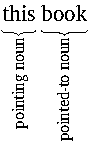
\includegraphics{A-Learners-Grammar-of-Classical-Standard-Arabic_files/figure-latex/unnamed-chunk-15-1.pdf}

The word \enquote{this} is what we will call a \emph{pointing noun}. We call it this because we can imagine standing next to a book and pointing to it and saying \enquote{this book}.

The word \enquote{book} here is similarly called the \emph{pointed-to} noun. It refers to the object being pointed to.

\section{The pointing nouns in Arabic}\label{the-pointing-nouns-in-arabic}

There are two types of pointing nouns:

\begin{enumerate}
\def\labelenumi{\roman{enumi}.}
\tightlist
\item
  Near pointing nouns: \enquote{this-one} (singular) and \enquote{these-ones} (dual and plural).
\item
  Far pointing nouns: \enquote{that-one} (singular) and \enquote{those-ones} (dual and plural).
\end{enumerate}

The following are the pointing nouns in Arabic:

\begin{longtable}[]{@{}
  >{\raggedright\arraybackslash}p{(\columnwidth - 10\tabcolsep) * \real{0.2174}}
  >{\raggedright\arraybackslash}p{(\columnwidth - 10\tabcolsep) * \real{0.0870}}
  >{\raggedleft\arraybackslash}p{(\columnwidth - 10\tabcolsep) * \real{0.1304}}
  >{\raggedright\arraybackslash}p{(\columnwidth - 10\tabcolsep) * \real{0.2174}}
  >{\raggedleft\arraybackslash}p{(\columnwidth - 10\tabcolsep) * \real{0.1304}}
  >{\raggedright\arraybackslash}p{(\columnwidth - 10\tabcolsep) * \real{0.2174}}@{}}
\toprule\noalign{}
\begin{minipage}[b]{\linewidth}\raggedright
Participant
\end{minipage} & \begin{minipage}[b]{\linewidth}\raggedright
State
\end{minipage} & \begin{minipage}[b]{\linewidth}\raggedleft
Near pointing noun
\end{minipage} & \begin{minipage}[b]{\linewidth}\raggedright
\end{minipage} & \begin{minipage}[b]{\linewidth}\raggedleft
Far pointing noun
\end{minipage} & \begin{minipage}[b]{\linewidth}\raggedright
\end{minipage} \\
\midrule\noalign{}
\endhead
\bottomrule\noalign{}
\endlastfoot
sing. masc. & all & \foreignlanguage{arabic}{هَـٰذَا} & this one\textsubscript{m} & \foreignlanguage{arabic}{ذَ~ٰلِکَ} & that one\textsubscript{m} \\
sing. fem. & all & \foreignlanguage{arabic}{هَـٰذِهِ} & this one\textsubscript{f} & \foreignlanguage{arabic}{تِلْکَ} & that one\textsubscript{f} \\
dual masc. & u & \foreignlanguage{arabic}{هَـٰذَانِ} & these ones\textsubscript{2,m} & \foreignlanguage{arabic}{ذَ~ٰنِکَ} & those ones\textsubscript{2,m} \\
dual masc. & a,i & \foreignlanguage{arabic}{هَـٰذَيْنِ} & these ones\textsubscript{2,m} & \foreignlanguage{arabic}{ذَيْنِکَ} & those ones\textsubscript{2,m} \\
dual fem. & u & \foreignlanguage{arabic}{هَاتَانِ} & these ones\textsubscript{2,f} & \foreignlanguage{arabic}{تَانِکَ} & those ones\textsubscript{2,f} \\
dual fem. & a,i & \foreignlanguage{arabic}{هَاتَيْنِ} & these ones\textsubscript{2,f} & \foreignlanguage{arabic}{تَيْنِکَ} & those ones\textsubscript{2,f} \\
plural & all & \foreignlanguage{arabic}{هَـٰؤُلَاءِ} & these ones\textsubscript{3} & \foreignlanguage{arabic}{أُولَـٰئِکَ} & those ones\textsubscript{3} \\
\end{longtable}

Note the following:

\begin{itemize}
\item
  Many of the pointing nouns contain small \foreignlanguage{arabic}{أَلِف} \foreignlanguage{arabic}{◌ٰ}. For most of them, this is how they must be written. It would be incorrect to write \foreignlanguage{arabic}{هَـٰذَا} \emph{hād͡hā} as \foreignlanguage{arabic}{هَاذَا}.
\item
  All the near pointing nouns begin with a \foreignlanguage{arabic}{ه}. And all the far pointing nouns end with \foreignlanguage{arabic}{ک}.
\item
  The \foreignlanguage{arabic}{و} in \foreignlanguage{arabic}{أُولَـٰئِکَ} \emph{ʾulāʾika} is silent and not pronounced. That is, the first syllable has a short vowel \emph{u}, not the long vowel \emph{ū}.
\item
  Most of the pointing nouns are rigid nouns. That is: their endings are not modified for their state.

  The dual pointing nouns, however, are flexible nouns, for example: \foreignlanguage{arabic}{هَـٰذَانِ} (u-state) / \foreignlanguage{arabic}{هَـٰذَيْنِ} \emph{hād͡hayni} (a- and i-states).
\item
  The pointing nouns for the plural are the same for both masculine and feminine genders.
\end{itemize}

\section{Definiteness of pointing nouns}\label{definiteness-of-pointing-nouns}

The pointing nouns share some similarities with pronouns \foreignlanguage{arabic}{هُوَ}, \foreignlanguage{arabic}{هِيَ}, etc. Just like pronouns, pointing nouns, too, are definite nouns even though they don't have \foreignlanguage{arabic}{ٱَلْ}.

Remember, however, from section~\ref{describers-with-annexations-to-pronouns}, that pronouns may not be describees.
Pointing nouns are different from pronouns in this regard. It is allowed to describe a pointing noun with a describer in a noun phrase.

Both these facts will prove useful in the next section.

\section{Pointing noun for plurals of non-intelligent beings}\label{pointing-noun-for-plurals-of-non-intelligent-beings}

Consistent with how we have been dealing with the so far,
, we can choose between the following pointing nouns for
the plurals of non-intelligent beings:

\begin{longtable}[]{@{}
  >{\raggedright\arraybackslash}p{(\columnwidth - 10\tabcolsep) * \real{0.2174}}
  >{\raggedright\arraybackslash}p{(\columnwidth - 10\tabcolsep) * \real{0.0870}}
  >{\raggedleft\arraybackslash}p{(\columnwidth - 10\tabcolsep) * \real{0.1304}}
  >{\raggedright\arraybackslash}p{(\columnwidth - 10\tabcolsep) * \real{0.2174}}
  >{\raggedleft\arraybackslash}p{(\columnwidth - 10\tabcolsep) * \real{0.1304}}
  >{\raggedright\arraybackslash}p{(\columnwidth - 10\tabcolsep) * \real{0.2174}}@{}}
\toprule\noalign{}
\begin{minipage}[b]{\linewidth}\raggedright
\end{minipage} & \begin{minipage}[b]{\linewidth}\raggedright
Near pointing noun
\end{minipage} & \begin{minipage}[b]{\linewidth}\raggedleft
Far pointing noun
\end{minipage} & \begin{minipage}[b]{\linewidth}\raggedright
\end{minipage} & \begin{minipage}[b]{\linewidth}\raggedleft
\end{minipage} & \begin{minipage}[b]{\linewidth}\raggedright
\end{minipage} \\
\midrule\noalign{}
\endhead
\bottomrule\noalign{}
\endlastfoot
sing. fem. & all & \foreignlanguage{arabic}{هَـٰذِهِ} & this one\textsubscript{f} & \foreignlanguage{arabic}{تِلْکَ} & that one\textsubscript{f} \\
plural & all & \foreignlanguage{arabic}{هَـٰؤُلَاءِ} & these ones\textsubscript{3} & \foreignlanguage{arabic}{أُولَـٰئِکَ} & those ones\textsubscript{3} \\
\end{longtable}

The singular feminine pointing noun is usually preferred, unless the plural plural pointing noun is needed to indicate that there is more than one.
We will be giving examples throughout this chapter.

\section{The pointing noun phrase}\label{the-pointing-noun-phrase}

Remember from chapter~\ref{adjectival-nouns-and-descriptive-noun-phrases} that a descriptive noun-phrase consists of a describer and a describee. The describer follows the describer and matches it in definiteness, state, gender, and number.

Here is an example of a descriptive noun-phrase in a sentence.

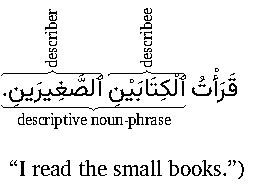
\includegraphics{A-Learners-Grammar-of-Classical-Standard-Arabic_files/figure-latex/unnamed-chunk-16-1.pdf}

We will now see how this same descriptive noun-phrase can be used with pointing nouns.

\subsection{Pointing to a single noun}\label{pointing-to-a-single-noun}

We will first deal with nouns that are single words, like \foreignlanguage{arabic}{ٱَلْکِتَابَيْنِ} above.
In section~\ref{pointing-to-an-annexation}
below, we will deal with nouns that are part of an annexation, like \foreignlanguage{arabic}{کِتَابَيِ ٱلرَّجُلِ}.

\subsubsection{\texorpdfstring{The pointed-to noun is definite with \foreignlanguage{arabic}{ٱَلْ}}{The pointed-to noun is definite with ٱَلْ}}\label{phrase-single-pointed-to-noun-with-al}

Just like an adjectival noun, a pointing noun can be a describer in a noun-phrase. But remember from
section~\ref{definiteness-of-pointing-nouns}
above that pointing nouns are definite.
So, if a pointing noun is a describer in a noun-phrase, the describee has to be definite too.
Example:

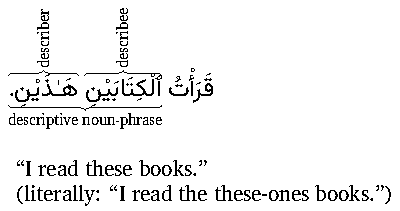
\includegraphics{A-Learners-Grammar-of-Classical-Standard-Arabic_files/figure-latex/unnamed-chunk-17-1.pdf}

In the above example, the pointed-to noun \foreignlanguage{arabic}{ٱَلْکِتَابَيْنِ} is the describee in a descriptive noun-phrase. It is definite, in the a-state, masculine, and dual.

The pointing noun \foreignlanguage{arabic}{هَـٰذَيْنِ} is its describer. It follows the describee and matches it being dual, in the a-state, masculine, and dual.

As a special case, when the pointed-to noun has \foreignlanguage{arabic}{ٱَلْ} (as in this case: \foreignlanguage{arabic}{ٱَلْکِتَابَيْنِ}), then the order of the pointing noun and the pointed to noun is permitted to be reversed.

The pointing noun is then a replacee (see section~\ref{the-replacement}), and the pointed-to noun is its replacement.

Example:

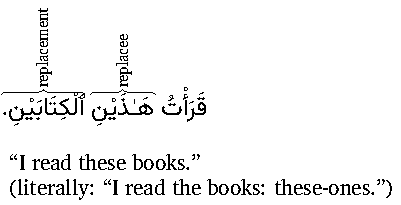
\includegraphics{A-Learners-Grammar-of-Classical-Standard-Arabic_files/figure-latex/unnamed-chunk-18-1.pdf}

In the above example, the
pointing noun \foreignlanguage{arabic}{هَـٰذَيْنِ}
is a replacee. It is definite, in the a-state, masculine, and dual.

The
pointed-to noun \foreignlanguage{arabic}{ٱَلْکِتَابَيْنِ}
is its replacement. It follows the replacee and matches it being dual, in the a-state, masculine, and dual.

As a matter of fact, even though both orders are permitted, this reverse order of placing the pointing noun first and following it with the pointed-to noun is more common.

Here are some more examples of pointing noun phrases when the pointed-to noun is definite with \foreignlanguage{arabic}{ٱَلْ}:

\foreignlanguage{arabic}{هَـٰذَا ٱَلرَّجُلُ ٱلْکَرِيمُ إِمَامٌ.}\\
\foreignlanguage{arabic}{ٱَلرَّجُلُ ٱلْکَرِيمُ هَـٰذَا إِمَامٌ.}\\
\enquote{This noble man is an imām.}

\subsubsection{The pointed-to noun is a proper noun}\label{the-pointed-to-noun-is-a-proper-noun}

Remember that proper noun are definite nouns, even though they usually don't begin with \foreignlanguage{arabic}{ٱَلْ}. For example:

\begin{longtable}[]{@{}rlrl@{}}
\toprule\noalign{}
\endhead
\bottomrule\noalign{}
\endlastfoot
\foreignlanguage{arabic}{زَيْد} & Zayd & \foreignlanguage{arabic}{ٱَلْحَارِث} & al-Ḥārit͡h \\
\textsuperscript{2}\foreignlanguage{arabic}{زَيْنَب} & Zaynab & \foreignlanguage{arabic}{قُرَيْش} & Qurays͡h \\
\end{longtable}

Such names may also be part of a pointing noun phrase.
If they don't begin with \foreignlanguage{arabic}{ٱَلْ} then only the {[}pointed-to noun first, then pointing noun{]} order is permitted.
Example:

\foreignlanguage{arabic}{زَيْدٌ هَـٰذَا أَخُو زَيْنَبَ تِلْکَ.}\\
\enquote{This Zayd is that Zaynab's brother.}

\foreignlanguage{arabic}{قُرَيْشٌ هَـٰؤُلَاءِ سَکَنُوا بِمَکَّةَ.}\\
\enquote{These Qurays͡h dwelled in Makkah.}

If the name begins with \foreignlanguage{arabic}{ٱَلْ} then both orders are permitted.

\foreignlanguage{arabic}{هَـٰذَا ٱلْحَارِث}\\
\foreignlanguage{arabic}{ٱلْحَارِث هَـٰذَا}\\
\enquote{this al-Ḥārit͡h}

\subsection{Pointing to an annexation}\label{pointing-to-an-annexation}

Consider the following expression:

\enquote{the man's book}

We can apply the pointing noun \enquote{this} to either \enquote{the book} or to \enquote{the man} in a pointing noun phrase. So we have two options:

\begin{enumerate}
\def\labelenumi{\roman{enumi}.}
\tightlist
\item
  \enquote{the book of this man}
\item
  \enquote{this book of the man}
\end{enumerate}

Similarly, consider the following expression:

\enquote{Zayd's book}

We can, again, apply the pointing noun \enquote{this} to either \enquote{the book} or to \enquote{Zayd}:

\begin{enumerate}
\def\labelenumi{\roman{enumi}.}
\tightlist
\item
  \enquote{the book of this Zayd}
\item
  \enquote{this book of Zayd}
\end{enumerate}

In this section we will learn how to construct these pointing noun phrases in Arabic.
Arabic uses annexations to express the above meanings. So we will discuss annexations like:

\foreignlanguage{arabic}{کِتَابُ ٱلرَّجُلِ}\\
\enquote{the book of the man}

and

\foreignlanguage{arabic}{کِتَابُ زَيْدٍ}\\
\enquote{the book of Zayd}

Note that both the above annexations are definite because their base nouns are definite.

Indefinite annexations like
\foreignlanguage{arabic}{کِتَاب رَجُلٍ} \enquote{a man's book}
cannot be used in pointing noun phrases.

\subsubsection{\texorpdfstring{The definite base noun begins with \foreignlanguage{arabic}{ٱَلْ}}{The definite base noun begins with ٱَلْ}}\label{the-definite-base-noun-begins-with-ux671ux644}

We will first consider annexations where the definite base noun begins with \foreignlanguage{arabic}{ٱَلْ}, like:

\foreignlanguage{arabic}{کِتَابُ ٱلرَّجُلِ}\\
\enquote{the book of the man}

\paragraph{Pointing to the base noun}\label{pointing-to-the-base-noun}

We would like to express the phrase:

\enquote{the book of this man}

In order to point to the base noun \foreignlanguage{arabic}{ٱَلرَّجُل} \enquote{the man} with the pointing noun \foreignlanguage{arabic}{هَـٰذَا} \enquote{this-one\textsubscript{m}}, we can put the pointing noun either before or after the base noun, thus:

\foreignlanguage{arabic}{کِتَابُ هَـٰذَا ٱلرَّجُلِ}\\
\foreignlanguage{arabic}{کِتَابُ ٱلرَّجُلِ هَـٰذَا}\\
\enquote{the book of this man}

Both these pointing noun phrases give the same meaning: \enquote{the book of this man}.
However, the first phrase
\foreignlanguage{arabic}{کِتَابُ هَـٰذَا ٱلرَّجُلِ}
is preferred, consistent with what we learned in
section~\ref{phrase-single-pointed-to-noun-with-al}, above.

The second phrase
\foreignlanguage{arabic}{کِتَابُ ٱلرَّجُلِ هَـٰذَا},
although correct, would only rarely be used with this meaning.
(In fact, it has another meaning: \enquote{this book of the man} which we will learn in
section~\ref{pointing-to-the-annexe-noun}, below.)

Here is how these phrases could be used in complete sentences:

\foreignlanguage{arabic}{کِتَابُ هَـٰذَا ٱلرَّجُلِ جَدِيدٌ.}\\
\foreignlanguage{arabic}{کِتَابُ ٱلرَّجُلِ هَـٰذَا جَدِيدٌ.}\\
\enquote{The book of this man is new.}

Before we give more examples, let's analyze these phrases in detail.

Consider the first pointing noun phrase:

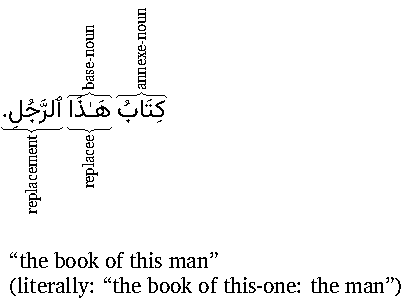
\includegraphics{A-Learners-Grammar-of-Classical-Standard-Arabic_files/figure-latex/unnamed-chunk-19-1.pdf}

As you can see the pointing noun
\foreignlanguage{arabic}{هَـٰذَا} has taken the place of
\foreignlanguage{arabic}{ٱَلرَّجُل} as the base noun in the annexation.
In addition to being the base noun,
\foreignlanguage{arabic}{هَـٰذَا} is also a replacee, whose replacement is
\foreignlanguage{arabic}{ٱَلرَّجُل}.
The literal, word-for-word, translation of this phrase is:

\enquote{the book of this-one: the man}

The more natural translation is:

\enquote{the book of this man}

Consider, now, the second pointing noun phrase:

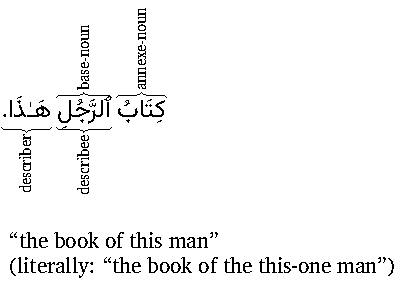
\includegraphics{A-Learners-Grammar-of-Classical-Standard-Arabic_files/figure-latex/unnamed-chunk-20-1.pdf}

\foreignlanguage{arabic}{ٱَلرَّجُل}, here, keeps its place as the base noun in the annexation.
In addition to being the base noun,
\foreignlanguage{arabic}{ٱَلرَّجُل}
is also a describee, whose describer is the pointing noun
\foreignlanguage{arabic}{هَـٰذَا}.
The literal, word-for-word, translation of this phrase is:

\enquote{the book of the this-one man}

The more natural translation is:

\enquote{the book of this man}

\paragraph{Pointing to the annexe noun}\label{pointing-to-the-annexe-noun}

Consider, again, the annexation:

\foreignlanguage{arabic}{کِتَابُ ٱلرَّجُلِ}\\
\enquote{the book of the man}

We have already discussed how to point to the base noun
\foreignlanguage{arabic}{ٱَلرَّجُل}
in a pointing noun phrase.
Now, we would like to point to the annexe noun
\foreignlanguage{arabic}{کِتَاب}
in a pointing noun phrase.

In other words, we would like to express the meaning:

\enquote{this book of the man}

The way to express this in Arabic is

\foreignlanguage{arabic}{کِتَابُ ٱلرَّجُلِ هَـٰذَا}\\
\enquote{this book of the man}

But wait! Didn't we see in section~\ref{pointing-to-the-base-noun} above that this expression has the meaning
\enquote{the book of this man}?

It turns out that this expression supports both meanings.

But it will generally only be used for the meaning: \enquote{this book of the man}

In order to express
\enquote{the book of this man}
we will typically use the expression \foreignlanguage{arabic}{کِتَابُ هَـٰذَا ٱلرَّجُلِ}.

Let's analyze the expression
\foreignlanguage{arabic}{کِتَابُ ٱلرَّجُلِ هَـٰذَا}
\enquote{this book of the man}
in detail:

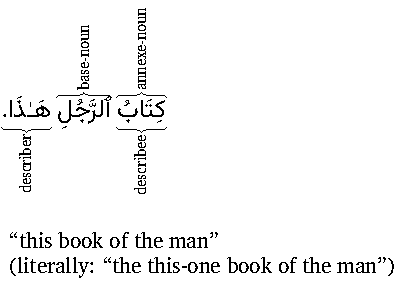
\includegraphics{A-Learners-Grammar-of-Classical-Standard-Arabic_files/figure-latex/unnamed-chunk-21-1.pdf}

\foreignlanguage{arabic}{کِتَاب}, here, is both and annexe noun and a describee.
Its describer is the pointing noun
\foreignlanguage{arabic}{هَـٰذَا}.
The literal, word-for-word, translation of this phrase is:

\enquote{the this-one book of the man}

The more natural translation is:

\enquote{this book of the man}

Here is this pointing noun phrase in a complete sentence:

\foreignlanguage{arabic}{کِتَابُ ٱلرَّجُلِ هَـٰذَا أَخْضَر.}\\
\enquote{This book of the man is green.}

\subparagraph*{Ambiguity of this phrase}\label{ambiguity-of-this-phrase}
\addcontentsline{toc}{subparagraph}{Ambiguity of this phrase}

A quick note about the ambiguity of this expression:

\foreignlanguage{arabic}{کِتَابُ ٱلرَّجُلِ هَـٰذَا}\\
\enquote{this book of the man} (usual)\\
\enquote{the book of this man} (rare)

The ambiguity of whether the pointing noun \foreignlanguage{arabic}{هَـٰذَا} points to the annexe noun
\foreignlanguage{arabic}{کِتَابُ}
or the base noun
\foreignlanguage{arabic}{ٱلرَّجُلِ}
only exists because the annexe noun and the base noun match each other in gender and number: singular masculine.
If the annexe noun and the base noun were different in gender and number, then there would be no ambiguity. Examples:

\foreignlanguage{arabic}{کِتَابَا ٱلرَّجُلِ هَـٰذَانِ}\\
\enquote{these books\textsubscript{2} of the man}

\foreignlanguage{arabic}{کِتَابُ ٱلرَّجُلَيْنِ هَـٰذَا}\\
\enquote{this book of the men\textsubscript{2}}

\foreignlanguage{arabic}{کِتَابُ ٱلْمَرْأَةِ هَـٰذَا}\\
\enquote{this book of the woman}

\foreignlanguage{arabic}{کِتَابُ ٱلْمَرْأَةِ هَـٰذِهِ}\\
\enquote{the book of this woman}

Here are some more examples of pointing to annexe nouns:

\paragraph{\texorpdfstring{The base noun is a proper noun beginning with \foreignlanguage{arabic}{ٱَلْ}}{The base noun is a proper noun beginning with ٱَلْ}}\label{the-base-noun-is-a-proper-noun-beginning-with-ux671ux644}

Consider the annexation:

\foreignlanguage{arabic}{کِتَابُ ٱلزُّبَيْرِ}\\
\enquote{the book of al-Zubayr}

We can apply the preceding discussion of pointing to the annexe noun and base noun to this annexation as well. So we get:

\foreignlanguage{arabic}{کِتَابُ هَـٰذَا ٱلزُّبَيْرِ}\\
\enquote{the book of this al-Zubayr}

\foreignlanguage{arabic}{کِتَابُ ٱلزُّبَيْرِ هَـٰذَا}\\
\enquote{this book of al-Zubayr} (usual)\\
\enquote{the book of this al-Zubayr} (rare)

\subsubsection{\texorpdfstring{The definite base noun does not begin with \foreignlanguage{arabic}{ٱَلْ}}{The definite base noun does not begin with ٱَلْ}}\label{the-definite-base-noun-does-not-begin-with-ux671ux644}

Consider, now, that the base noun is definite but does not begin with \foreignlanguage{arabic}{ٱَلْ}. There are two such types of nouns that we will discuss:

\begin{enumerate}
\def\labelenumi{\roman{enumi}.}
\tightlist
\item
  Proper nouns not beginning with \foreignlanguage{arabic}{ٱَلْ}
\item
  Pronouns
\end{enumerate}

\paragraph{\texorpdfstring{The base noun is a proper noun not beginning with \foreignlanguage{arabic}{ٱَلْ}}{The base noun is a proper noun not beginning with ٱَلْ}}\label{the-base-noun-is-a-proper-noun-not-beginning-with-ux671ux644}

We will first deal with proper nouns that don't begin with \foreignlanguage{arabic}{ٱَلْ}.
Consider the annexation:

\foreignlanguage{arabic}{کِتَابُ زَيْدٍ}\\
\enquote{the book of Zayd}

Because the base noun \foreignlanguage{arabic}{زَيْد} does not begin with \foreignlanguage{arabic}{ٱَلْ}, any pointing nouns can come only after the entire annexation, thus:

\foreignlanguage{arabic}{کِتَابُ زَيْدٍ هَـٰذَا}

In theory, this supports two meanings:

\begin{enumerate}
\def\labelenumi{\roman{enumi}.}
\tightlist
\item
  \enquote{this book of Zayd}
\item
  \enquote{the book of this Zayd}
\end{enumerate}

In practice, however, the first meaning
(\enquote{this book of Zayd})
is much more likely.
Pointing to a proper noun in a pointing noun phrase
(\enquote{the book of this Zayd})
is uncommon, generally.

\paragraph{The base noun is a pronoun}\label{the-base-noun-is-a-pronoun}

We have learned, in
section~\ref{definiteness-of-pronouns},
that pronouns are always definite, despite not beginning with \foreignlanguage{arabic}{ٱَلْ}.

We have also learned, in
section~\ref{pronouns-as-base-nouns},
that a pronoun may be a base noun in an annexation.
Example:

\foreignlanguage{arabic}{کِتَابُهُ}\\
\enquote{his book}

Neither the annexe noun \foreignlanguage{arabic}{کِتَاب}, nor the attached pronoun \foreignlanguage{arabic}{هُ} begin with \foreignlanguage{arabic}{ٱَلْ}.
So if we want to add the pointing noun \foreignlanguage{arabic}{هَـٰذَا} to this annexation to form a pointing noun phrase,
then we have to place it at the end, after the annexation, thus:

\foreignlanguage{arabic}{کِتَابُهُ هَـٰذَا}

The pointing noun \foreignlanguage{arabic}{هَـٰذَا}, here, is a describee. But what is its describer?

We have also learned, in
section~\ref{describers-with-annexations-to-pronouns}
that pronouns may not be describees in a descriptive noun phrase.

So, we are left with only one option: the annexe noun \foreignlanguage{arabic}{کِتَاب} is the desceibee. And the meaning of the phrase is:

\foreignlanguage{arabic}{کِتَابُهُ هَـٰذَا}\\
\enquote{this book of his}

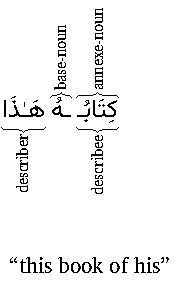
\includegraphics{A-Learners-Grammar-of-Classical-Standard-Arabic_files/figure-latex/unnamed-chunk-22-1.pdf}

Here are some more examples:

\section{Pointing nouns as subjects}\label{pointing-nouns-as-subjects}

Besides their use in pointing noun phrases, pointing nouns are very often used as the subject of a sentence. For example:

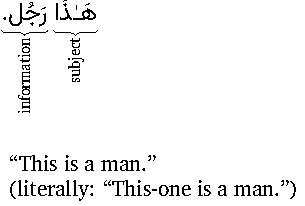
\includegraphics{A-Learners-Grammar-of-Classical-Standard-Arabic_files/figure-latex/unnamed-chunk-23-1.pdf}

The pointing noun is (usually) made to match the information in number and gender. Examples:

\foreignlanguage{arabic}{هَاتَانِ جَارِيَتَانِ.}\\
\enquote{These are girls\textsubscript{2}.}

\foreignlanguage{arabic}{أُولَـٰئِکَ مُعَلِّمُونَ.}\\
\enquote{Those are teachers.}

\foreignlanguage{arabic}{هَـٰؤُلَاءِ أَقْلَامٌ.}\\
\enquote{These are pens.}

\foreignlanguage{arabic}{تِلْکَ بُيُوتٌ.}\\
\enquote{Those are houses.}

\foreignlanguage{arabic}{هَـٰذَانِ صَغِيرَانِ.}\\
\enquote{These are small ones\textsubscript{2}.}

The information may be a single word (as above) or more complex (as below):

\foreignlanguage{arabic}{ذَ~ٰلِکَ أَمِيرُ ٱلْمُؤِْمِنِينَ.}\\
\enquote{That is the commander of the believers.}

\foreignlanguage{arabic}{أُولَـٰئِکَ أَکَلْنَ ٱلطَّعَامَ..}\\
\enquote{Those-ones ate\textsubscript{3,f} the food.}

\foreignlanguage{arabic}{هَـٰذَا ثَوْبُ رَجُلٍ.}\\
\enquote{This is a man's garment.}

\foreignlanguage{arabic}{هَـٰذِهِ کُتُبُهُ.}\\
\enquote{These are his books.}

\foreignlanguage{arabic}{هَـٰذَانِ بَيْتَانِ کَبِيرَانِ..}\\
\enquote{These are big houses\textsubscript{2}.}

If the information is a noun that begins with \foreignlanguage{arabic}{ٱَلْ} then it may be placed after the pointing noun subject in the same manner:

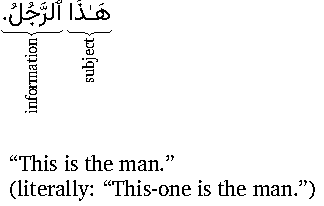
\includegraphics{A-Learners-Grammar-of-Classical-Standard-Arabic_files/figure-latex/unnamed-chunk-24-1.pdf}

While the this is permitted and correct, it may be sometimes confused with for the pointing noun phrase \enquote{this man}. So, in the same way that we learned in
section~\ref{chap-smp-sent-sec-def-info},
we insert a detached pronoun between the subject and the information, thus:

\foreignlanguage{arabic}{هَـٰذَا هُوَ ٱلرَّجُلُ.}\\
\enquote{This is the man.}

Here are some more examples:

\foreignlanguage{arabic}{هَاتَانِ هُمَا ٱلْجَارِيَتَانِ.}\\
\enquote{These are the girls\textsubscript{2}.}

\foreignlanguage{arabic}{أُولَـٰئِکَ هُمُ ٱلْمُعَلِّمُونَ.}\\
\enquote{Those are the teachers.}

\foreignlanguage{arabic}{هَـٰؤُلَاءِ هُنَّ ٱلْأَقْلَامٌ.}\\
\enquote{These are the pens.}

\foreignlanguage{arabic}{تِلْکَ هِيَ ٱلْبُيُوتٌ.}\\
\enquote{Those are the houses.}

\foreignlanguage{arabic}{هَـٰذَانِ هُمَ ٱلصَّغِيرَانِ.}\\
\enquote{These are the small ones\textsubscript{2}.}

\subsection{Mismatched pointing noun subject}\label{mismatched-pointing-noun-subject}

When the pointing noun is a subject we usually match its number and gender with the number and gender of the information, as we have been doing so far. However, when the pointing noun subject refers to a noun in a previous sentence, then we may prefer to match to the previous noun than to the the following information. Example:

\foreignlanguage{arabic}{بَلَغَنَا خَبَرُ ٱلْمَطَرِ عَلَى ٱلْجَبَالِ. ذَ~ٰلِکَ بُشْرَىٰ لِلزُّرَّاعِ.}\\
\enquote{The news of the rain on the mountains has reached us. That is a good tiding for the sowers.}

Note that the second sentence's subject and information mismatch:

\foreignlanguage{arabic}{ذَ~ٰلِکَ بُشْرَىٰ}\\
\enquote{That is a good tiding.}

The information
\foreignlanguage{arabic}{بُشٌرَىٰ} \enquote{a good tiding} is a feminine noun but the subject
\foreignlanguage{arabic}{ذَ~ٰلِکَ} is masculine.
This is because
\foreignlanguage{arabic}{ذَ~ٰلِکَ}
is actually referring to \foreignlanguage{arabic}{خَبَر} in the previous sentence which is a masculine noun.

\section{Pointing nouns as other parts of speech}\label{pointing-nouns-as-other-parts-of-speech}

Besides their use in pointing noun phrases and as subjects, pointing nouns may be used as other parts of speech as well, typically where one would expect pronouns. Here are some examples:

\foreignlanguage{arabic}{أَخَذْتُ ٱلْکِتَابَيْنِ مِنَ ٱلْمَکْتَبَةِ. قَرَأْتُ هَـٰذا وَمَا قَرَأْتُ ذَ~ٰلِکَ.}\\
\enquote{I took the books\textsubscript{2} from the library. I read this one and I didn't read that one.}

\foreignlanguage{arabic}{شَغَلَنِي ٱلْعَمَلُ ٱلصَّعْبُ وَمَا فَرَغْتُ مِنْ ذَ~ٰلِکَ.}\\
\enquote{The difficult work occupied me and I did not get done with that.}

\chapter{u-state incomplete-action verbs}\label{u-state-incomplete-action-verbs}

\section{Introduction}\label{introduction-15}

We had mentioned that there are approximately 10 commonly used verb forms. And we have already studied the completed-action verb for form 1. In this chapter we will study incomplete-action form 1 verbs. Incomplete-action verbs are used when the action of a verb is on-going at present or will occur in the future.

\section{Pattern for form 1}\label{pattern-for-form-1}

Using the root paradigm \foreignlanguage{arabic}{«فعل»}, we have already seen that completed-action verbs for form 1 occur in the patterns \foreignlanguage{arabic}{فَعَلَ} \emph{faɛala}, \foreignlanguage{arabic}{فَعِلَ} \emph{faɛila}, and \foreignlanguage{arabic}{فَعُلَ} \emph{faɛula}. The patterns for form 1 incomplete-action verbs are \foreignlanguage{arabic}{يَفْعَلُ} \emph{yafɛalu}, \foreignlanguage{arabic}{يَفْعِلُ} \emph{yafɛilu}, and \foreignlanguage{arabic}{يَفْعُلُ} \emph{yafɛulu}.

Note that the incomplete-action verb forms add an extraneous \foreignlanguage{arabic}{يَـ} \emph{ya-} to the beginning of the verb. This extra letter can change, as we will see soon, to the letters \foreignlanguage{arabic}{تَـ} \emph{ta-}, \foreignlanguage{arabic}{نَـ} \emph{na}, or \foreignlanguage{arabic}{أَ} \emph{ʾa-} depending on the doer.

\section{Vowel-mark on the middle root letter}\label{vowel-mark-on-the-middle-root-letter}

We have seen that vowel on the middle root letter in a completed-action verb can vary depending on the verb. So we can have,

\begin{itemize}
\tightlist
\item
  \foreignlanguage{arabic}{کَتَبَ} \emph{kataba} \enquote{he wrote}
\item
  \foreignlanguage{arabic}{عَمِلَ} \emph{ɛamila} \enquote{he worked}
\item
  \foreignlanguage{arabic}{کَبُرَ} \emph{kabura} \enquote{he became big}
\end{itemize}

Similarly, the vowel on the middle letter in an incomplete-action verb can also vary depending on the verb. Generally, this will need to be looked up in a dictionary and memorized. But there are the following rules which limit the variation:

\begin{enumerate}
\def\labelenumi{\arabic{enumi}.}
\item
  If the completed-action verb has an \emph{a}-mark on the middle letter, the incomplete-action verb's middle letter can have either an \emph{a}-mark, \emph{i}-mark, or an \emph{u}-mark, depending on the verb. For example,

  \begin{itemize}
  \tightlist
  \item
    \foreignlanguage{arabic}{کَتَبَ يَکْتُبُ} \emph{kataba yaktubu} \enquote{he wrote, he writes}
  \item
    \foreignlanguage{arabic}{ذَهَبَ يَذْهَبُ} \emph{d͡hahaba yad͡h·habu} \enquote{he went, he goes}
  \item
    \foreignlanguage{arabic}{کَشَفَ يَکْشِفُ} \emph{kas͡hafa yaks͡hifu} \enquote{he uncovered, he uncovers}
  \end{itemize}
\item
  If the completed-action verb has an \emph{i}-mark on the middle letter, the incomplete-action verb's middle letter will usually have an \emph{a}-mark. Rarely, for a few verbs, it may be an \emph{i}-mark instead. For example,

  \begin{itemize}
  \tightlist
  \item
    \foreignlanguage{arabic}{عَمِلَ يَعْمَلُ} \emph{ɛamila yaɛmalu} \enquote{he worked, he works}
  \item
    \foreignlanguage{arabic}{حَسِبَ يَحْسِبُ} \emph{ḥasiba yaḥsibu} \enquote{he deemed, he deems}
  \end{itemize}
\item
  If the completed-action verb has an \emph{u}-mark on the middle letter, the incomplete-action verb's middle letter shall have a \emph{u}-mark. For example,

  \begin{itemize}
  \tightlist
  \item
    \foreignlanguage{arabic}{کَبُرَ يَکْبُرُ} \emph{kabura yakburu} \enquote{he grew big, he grows big}
  \end{itemize}
\end{enumerate}

It is possible for some incomplete-action verbs to have more than option for the vowel mark on the middle letter. Both variants give the same meaning for the verb. For example, the completed-action verb \foreignlanguage{arabic}{حَسِبَ} \emph{ḥasiba} \enquote{he deemed} has as its incomplete-verb both \foreignlanguage{arabic}{يَحْسِبُ} \emph{yaḥsibu} and \foreignlanguage{arabic}{يَحْسَبُ} \emph{yaḥsabu}.

\section{Verb state}\label{verb-state}

As you know, nouns in Arabic have a state that is determined by the function of the noun in the sentence. For example, consider the following sentence:

\foreignlanguage{arabic}{سَأَلَ ٱلْغُلَامُ ٱلرَّجُلَ عَنْ شَيْءٍ.}\\
\emph{saʾala -lg͡hulāmu -rrajula ʾan s͡hayʾin.}\\
\enquote{The boy asked the man about something.}

In the above sentence, \foreignlanguage{arabic}{ٱَلْغُلَامُ} \emph{ʾalg͡hulāmu} is the doer of the verb so it is in the u-state and this is indicated by the \emph{u}-mark on its final letter.
\foreignlanguage{arabic}{ٱَلرَّجُلَ} \emph{ʾarrujala} is the direct doee of the verb so it is in the a-state and this is indicated by the \emph{a}-mark on its final letter.
\foreignlanguage{arabic}{شَيْءٍ} \emph{s͡hayʾin} is directly preceded by a preposition so it is in the i-state and this is indicated by the nūnated \emph{i}-mark \foreignlanguage{arabic}{◌ٍ} on its final letter.
The ending of the completed-action verb \foreignlanguage{arabic}{سَأَلَ} is not determined based on the function of the verb in the sentence, and therefore, it does not have any state. (Its ending can change depending on whether a pronoun is attached to it but this is not related to the function of the verb in the sentence and does not represent any state.)

As opposed to completed-action verbs, which don't have any state, incomplete-action verbs do have a state which is determinined by the function of the verb in a sentence. Similar to nouns, the state of an incomplete-action verb is indicated by the vowel mark or suffix at the end of the verb.

Incomplete action verbs have three states, just like nouns. These states are called:

\begin{enumerate}
\def\labelenumi{\roman{enumi}.}
\tightlist
\item
  The u-state
\item
  The a-state
\item
  The ø-state
\end{enumerate}

Two of the states have their names in common with nouns: the u-state and the a-state. The the ø-state (null-state) is named differently.

The \emph{u}-mark on the final letter of \foreignlanguage{arabic}{يَفُعَلُ} \emph{yafɛalu} indicates that it is in the u-state. We will study only the u-state of incomplete-action verbs in this chapter. And we will study the a-state and ø-state in later chapters if Allāh wills.

\section{With doer nouns}\label{with-doer-nouns}

As with completed-action verbs, doer nouns are placed after the verb in sentence word order. However, the gender of the doer noun affects the beginning of the incomplete-action verb. If the doer noun is masculine, then the incomplete-action verb shall begin with used is \foreignlanguage{arabic}{يَـ} \emph{ya-}. And if the doer noun is feminine, then the incomplete-action verb shall begin with \foreignlanguage{arabic}{تَـ} \emph{ta-}. Examples:

\foreignlanguage{arabic}{يَکْتُبُ ٱلْغُلَامُ فِي کِتابِهِ.}\\
\emph{yaktubu -lg͡hulāmu fī kitābihi}\\
\enquote{The boy writes in his book.}

\foreignlanguage{arabic}{يَعْمَلُ ٱلرَّجُلَانِ فِي ٱلْمَدِينَةِ.}\\
\emph{yaɛmalu -rrajulāni fi -lmadīnati.}\\
\enquote{The men\textsubscript{dual.} work in the city.}

\foreignlanguage{arabic}{يَکْتُبُ ٱلْجَارِيَةُ فِي کِتابِهَا.}\\
\emph{yaktubu -ljāriyatu fī kitābihā.}\\
\enquote{The girl writes in her book.}

\foreignlanguage{arabic}{تَعْمَلُ ٱلنِّسَاءُ فِي بُيُوتِهِنَّ.}\\
\emph{taɛmalu -nnisāʾu fī buyūtihinna.}\\
\enquote{The women work in their houses.}

\section{With doee nouns and pronouns}\label{with-doee-nouns-and-pronouns}

Doee nouns and pronouns with incomplete-action verbs work exactly as with completed-action verbs.

\foreignlanguage{arabic}{يَسْأَلُ ٱلْغُلَامُ ٱلرَّجُلَ سُؤَالًا.}\\
\emph{yasʾalu -lg͡hulāmu -rrajula suʾālan.}\\
\enquote{The boy asks the man a question.}

\foreignlanguage{arabic}{يَسْأَلُهَا ٱلْغُلَامُ سُؤَالًا.}\\
\emph{yasʾaluha -lg͡hulāmu suʾālan.}\\
\enquote{The boy asks her a question.}

\section{With doer pronouns}\label{with-doer-pronouns}

When we studied completed-action verbs, we saw that doer pronouns are either visible or invisible. Visible doer pronouns are added to the end of the verb, modifying the end of the verb in the process.

The doer pronouns for incomplete-action verbs are different from the doer pronouns for completed-action verbs.
Incomplete-action verbs' doer pronouns are also added to the end of the verb, but in addition to modifying the end of the verb, they modify the beginning of the verb as well. Futhermore, additional letters may be added after the doer pronoun to indicate the state of the verb.

We'll show what all this means in the table below of verbs with doer pronouns. Completed-action verbs are included as well so that you can contrast them with their incomplete-action counterparts.

\begin{longtable}[]{@{}
  >{\raggedright\arraybackslash}p{(\columnwidth - 8\tabcolsep) * \real{0.2000}}
  >{\raggedright\arraybackslash}p{(\columnwidth - 8\tabcolsep) * \real{0.1500}}
  >{\raggedright\arraybackslash}p{(\columnwidth - 8\tabcolsep) * \real{0.2500}}
  >{\raggedright\arraybackslash}p{(\columnwidth - 8\tabcolsep) * \real{0.1500}}
  >{\raggedright\arraybackslash}p{(\columnwidth - 8\tabcolsep) * \real{0.2500}}@{}}
\toprule\noalign{}
\begin{minipage}[b]{\linewidth}\raggedright
Person
\end{minipage} & \begin{minipage}[b]{\linewidth}\raggedright
Completed-action doer pronoun
\end{minipage} & \begin{minipage}[b]{\linewidth}\raggedright
Completed-action verb with doer pronoun
\end{minipage} & \begin{minipage}[b]{\linewidth}\raggedright
Incomplete-action verb doer pronoun
\end{minipage} & \begin{minipage}[b]{\linewidth}\raggedright
Incomplete-action verb with doer pronoun in the u-state
\end{minipage} \\
\midrule\noalign{}
\endhead
\bottomrule\noalign{}
\endlastfoot
he & \emph{invisible} & \foreignlanguage{arabic}{فَعَلَ} \emph{faɛala} & \emph{invisible} & \foreignlanguage{arabic}{يَفْعَلُ} \emph{yafɛalu} \\
she & \emph{invisible} & \foreignlanguage{arabic}{فَعَلَتْ} \emph{faɛalat} & \emph{invisible} & \foreignlanguage{arabic}{تَفْعَلُ} \emph{tafɛalu} \\
you\textsubscript{1,m} & \foreignlanguage{arabic}{تَ} \emph{-ta} & \foreignlanguage{arabic}{فَعَلْتَ} \emph{faɛalta} & \emph{invisible} & \foreignlanguage{arabic}{تَفْعَلُ} \emph{tafɛalu} \\
you\textsubscript{1,f} & \foreignlanguage{arabic}{تِ} \emph{-ti} & \foreignlanguage{arabic}{فَعَلْتِ} \emph{faɛalti} & \foreignlanguage{arabic}{ي} \emph{-ī} & \foreignlanguage{arabic}{تَفْعَلِينَ} \emph{tafɛalīna} \\
I & \foreignlanguage{arabic}{تُ} \emph{tu} & \foreignlanguage{arabic}{فَعَلْتُ} \emph{faɛaltu} & \emph{invisible} & \foreignlanguage{arabic}{أَفْعَلُ} \emph{ʾafɛalu} \\
they\textsubscript{2,m} & \foreignlanguage{arabic}{ا} \emph{-ā} & \foreignlanguage{arabic}{فَعَلَا} \emph{faɛalā} & \foreignlanguage{arabic}{ا} \emph{-ā} & \foreignlanguage{arabic}{يَفْعَلَانِ} \emph{yafɛalāni} \\
they\textsubscript{2,f} & \foreignlanguage{arabic}{ا} \emph{-ā} & \foreignlanguage{arabic}{فَعَلَتَا} \emph{faɛalatā} & \foreignlanguage{arabic}{ا} \emph{-ā} & \foreignlanguage{arabic}{تَفْعَلَانِ} \emph{tafɛalāni} \\
you\textsubscript{2} & \foreignlanguage{arabic}{تُمَا} \emph{-tumā} & \foreignlanguage{arabic}{فَعَلْتُمَا} \emph{faɛaltumā} & \foreignlanguage{arabic}{ا} \emph{-ā} & \foreignlanguage{arabic}{تَفْعَلَانِ} \emph{tafɛalāni} \\
they\textsubscript{3+,m} & \foreignlanguage{arabic}{و} \emph{-ū} & \foreignlanguage{arabic}{فَعَلُوا} \emph{faɛalū} & \foreignlanguage{arabic}{و} \emph{-ū} & \foreignlanguage{arabic}{يَفْعَلُونَ} \emph{yafɛalūna} \\
they\textsubscript{3+,f} & \foreignlanguage{arabic}{نَ} \emph{-na} & \foreignlanguage{arabic}{فَعَلْنَ} \emph{faɛalna} & \foreignlanguage{arabic}{نَ} \emph{-na} & \foreignlanguage{arabic}{يَفْعَلْنَ} \emph{yafɛalna} \\
you\textsubscript{3+,m} & \foreignlanguage{arabic}{تُمْ} \emph{-tumā} & \foreignlanguage{arabic}{فَعَلْتُمْ} \emph{faɛaltum} & \foreignlanguage{arabic}{و} \emph{-ū} & \foreignlanguage{arabic}{تَفْعَلُونَ} \emph{tafɛalūna} \\
you\textsubscript{3+,f} & \foreignlanguage{arabic}{تُنَّ} \emph{-tunna} & \foreignlanguage{arabic}{فَعَلْتُنَّ} \emph{faɛaltunna} & \foreignlanguage{arabic}{نَ} \emph{na} & \foreignlanguage{arabic}{تَفْعَلْنَ} \emph{tafɛalna} \\
we & \foreignlanguage{arabic}{نَا} \emph{nā} & \foreignlanguage{arabic}{فَعَلْنَا} \emph{faɛalnā} & \emph{invisible} & \foreignlanguage{arabic}{نَفْعَلُ} \emph{nafɛalu} \\
\end{longtable}

Note the following:

\begin{itemize}
\tightlist
\item
  The verb \foreignlanguage{arabic}{تَفْعَلُ} is used both for \enquote{she} and \enquote{you\textsubscript{2m}} doers. Only context will be able to help us differentiate between the two.
\item
  In incomplete action verbs which have invisible doer pronouns, the u-state of the verb is indicated by the \emph{u}-mark \foreignlanguage{arabic}{◌ُ} on the final letter of the verb.
\item
  For incomplete-action verbs that have \foreignlanguage{arabic}{ا}, \foreignlanguage{arabic}{و}, or \foreignlanguage{arabic}{ي} as the doer pronoun, the u-state is indicated by an extraneous \foreignlanguage{arabic}{ن} added to the end of the verb.
\item
  And for the remaining incomplete action verbs whose doer pronoun is \foreignlanguage{arabic}{نَ}, there is no indication of the state of the verb.
\end{itemize}

Here are some examples of the usage of the doer pronouns:

Remember that in Arabic, each verb must have it's own doer, so when there are multiple verbs associated with the same doer, the first verb can be used with the doer noun and the rest with doer pronouns. This is the same behavior as with completed-action verbs. For example:

\foreignlanguage{arabic}{يَجْلِسُ ٱلرِّجَالُ وَيَأْکُلُونَ وَيَشْرَبُونَ.}\\
\emph{yajlisu -rrijālu wa yaʾkulūna wa yas͡hrabūna.}\\
\enquote{The men sit and (they) eat and (they) drink.}

\section{Future}\label{future}

The incomplete-action verb is used to express both the present (habitual and progressive) and future tenses. Sometimes all meanings are meant in the same expression. And if only one of the meanings is intended, context can be sufficient to determine which is intended. So, for example,

\foreignlanguage{arabic}{يَذْهَبُ ٱلرَّجُلُ}\\
\emph{yad͡h·habu -rrajulu.}

can mean, either one, or even all, of:

\enquote{The man goes.} or\\
\enquote{The man is going.} or\\
\enquote{The man will go.}

Arabic does provide a mechanism for specifying that the use of an incomplete-action verb is solely to intend a future action. This is by means of the particles \foreignlanguage{arabic}{سَـ} \emph{sa-} and \foreignlanguage{arabic}{سَوْفَ} \emph{sawfa} that can be placed before the verb. They provide a meaning of \enquote{will} or \enquote{will soon}. \foreignlanguage{arabic}{سَـ} \emph{sa-}, being a single letter particle, is attached to the verb.

For example,

\foreignlanguage{arabic}{سَيَذْهَبُ ٱلرَّجُلُ}\\
\emph{sayad͡h·habu -rrajulu.}\\
and\\
\foreignlanguage{arabic}{سَوْفَ يَذْهَبُ ٱلرَّجُلُ}\\
\emph{sawfa yad͡h·habu -rrajulu.}\\
\enquote{The man will go.} or\\
\enquote{Soon the man will go.}

The difference in usage of \foreignlanguage{arabic}{سَـ} \emph{sa-} and \foreignlanguage{arabic}{سَوْفَ} \emph{sawfa} can be thought of as one of emphasis. \foreignlanguage{arabic}{سَوْفَ} \emph{sawfa} is more emphatic than \foreignlanguage{arabic}{سَـ} \emph{sa-}. This emphasis can translate to more definiteness in the action or even that the action is farther in the future.

\section{Negation}\label{negation}

\subsection{\texorpdfstring{Negation using \foreignlanguage{arabic}{مَا} \emph{mā}}{Negation using مَا mā}}\label{negation-using-ux645ux627-ma}

As with completed-action verbs, incomplete-action verbs too can be negated by placing the particle \foreignlanguage{arabic}{مَا} before them. This negates the meaning of the verb usually for the present tense. For example,

\foreignlanguage{arabic}{مَا يَذْهَبُ ٱلرَّجُلُ}\\
\emph{mā yad͡h·habu -rrajulu.}\\
\enquote{The man does not go.} or,\\
\enquote{The man is not going.}

\subsection{\texorpdfstring{Negation using \foreignlanguage{arabic}{لَا} \emph{lā}}{Negation using لَا lā}}\label{u-state-verb-negation-la}

In addition to \foreignlanguage{arabic}{مَا} \emph{mā}, incomplete-action verbs can be negated using \foreignlanguage{arabic}{لَا} \emph{lā} in the same manner. In addition to negating the meaning of the verb for the present tense, it can also negate the meaning for the future tense.

\foreignlanguage{arabic}{لَا يَذْهَبُ ٱلرَّجُلُ}\\
\emph{lā yad͡h·habu -rrajulu.}\\
\enquote{The man does not go.} or,\\
\enquote{The man is not going.} or,\\
\enquote{The man will not go.}

The particles \foreignlanguage{arabic}{سَـ} \emph{sa-} and \foreignlanguage{arabic}{سَوْفَ} \emph{sawfa} may not be combined with \foreignlanguage{arabic}{مَا} \emph{mā} and \foreignlanguage{arabic}{لَا} \emph{lā} when negating verbs.

\section{\texorpdfstring{With \foreignlanguage{arabic}{قَدْ}}{With قَدْ}}\label{with-ux642ux62f}

TODO

When negating a resembling verb preceded by
\foreignlanguage{arabic}{قَدْ}
there is some question about whether \foreignlanguage{arabic}{قَدْ} is retained or dropped,
but the stronger opinion seems to be that it may be kept, as proven by the following verse of poetry:

\foreignlanguage{arabic}{وَقَدْ لَا تَعْدَمُ الْحَسْنَاءُ ذَامًا}\\
\enquote{And {[}it{]} may be {[}that{]} the beautiful female does not lack a defect.}\\
(\foreignlanguage{arabic}{ذَام} means \enquote{defect}.)

\chapter{The verbal-noun of doing}\label{the-verbal-noun-of-doing}

\section{Introduction}\label{introduction-16}

Every verb has a set of \emph{verbal-nouns} derived from it that, despite being nouns, have a verbal meaning to them. One of these verbal-nouns is the \enquote{doing} verbal-noun, that we shall study in this chapter.

Consider the following form~1 verb:

\begin{longtable}[]{@{}
  >{\raggedright\arraybackslash}p{(\columnwidth - 6\tabcolsep) * \real{0.1579}}
  >{\raggedright\arraybackslash}p{(\columnwidth - 6\tabcolsep) * \real{0.2632}}
  >{\raggedright\arraybackslash}p{(\columnwidth - 6\tabcolsep) * \real{0.3158}}
  >{\raggedright\arraybackslash}p{(\columnwidth - 6\tabcolsep) * \real{0.2632}}@{}}
\toprule\noalign{}
\begin{minipage}[b]{\linewidth}\raggedright
Root
\end{minipage} & \begin{minipage}[b]{\linewidth}\raggedright
Completed-action verb
\end{minipage} & \begin{minipage}[b]{\linewidth}\raggedright
Incomplete-action verb (u-state)
\end{minipage} & \begin{minipage}[b]{\linewidth}\raggedright
Doing verbal-noun
\end{minipage} \\
\midrule\noalign{}
\endhead
\bottomrule\noalign{}
\endlastfoot
\foreignlanguage{arabic}{«ذهب»} & \foreignlanguage{arabic}{ذَهَبَ} \enquote{he went} & \foreignlanguage{arabic}{يَذْهَبُ} \enquote{he goes} & \foreignlanguage{arabic}{ذَهَاب} \enquote{going} \\
\end{longtable}

The doing verbal-noun associated with this verb is \foreignlanguage{arabic}{ذَهَاب} \emph{d͡hahāb}. It denotes \enquote{the action of going}, or simply \enquote{going}. In this section we shall learn how this and other verbal-nouns are used.

Before we proceed, we present a new method to present a verb and its meaning in this book.
We will often give a new verb in the format:

\foreignlanguage{arabic}{ذَهَبَ يَذْهَبُ ذَهَابًا} \enquote{to go}

The completed-action verb for the singular masculine absentee participant \enquote{he}, the corresponding incomplete-action verb, and their doing verbal-noun are given together, in sequence. The doing verbal-noun is given in the a-state, because of a usage that we shall learn in a later chapter, if Allāh wills. This is how verb definitions are traditionally found in Arabic dictionaries. And the English meaning is given using the dictionary definition, in this case, the phrase: \enquote{to go}.

\section{Patterns of the doing verbal-noun for form~1 verbs}\label{patterns-of-the-doing-verbal-noun-for-form-1-verbs}

The patterns of the doing verbal-noun for form~1 verbs are very variable. It is best to learn the doing verbal-noun when you learn a new verb. Having said that, there are some general trends which may be useful to keep in mind:

\begin{enumerate}
\def\labelenumi{\arabic{enumi}.}
\tightlist
\item
  If the verb takes a direct doee, then the completed-action verb must necessarily be of the pattern \foreignlanguage{arabic}{فَعَلَ} \emph{faɛala} or \foreignlanguage{arabic}{فَعِلَ} \emph{faɛila} (because completed-action verbs of the pattern \foreignlanguage{arabic}{فَعُلَ} \emph{faɛula} never take a direct doee). In this case:

  \begin{enumerate}
  \def\labelenumii{\alph{enumii}.}
  \tightlist
  \item
    The doing verbal-noun for many verbs, in general, tends to be \foreignlanguage{arabic}{فَعْل} \emph{faɛl}. Examples:

    \begin{itemize}
    \tightlist
    \item
      \foreignlanguage{arabic}{فَتَحَ يَفْتَحُ فَتْحًا} \enquote{to open (\foreignlanguage{arabic}{هـ} s.th.)}
    \item
      \foreignlanguage{arabic}{أَخَذَ يَأْخُذُ أَخْذًا} \enquote{to take (\foreignlanguage{arabic}{هـ} s.th.)}
    \item
      \foreignlanguage{arabic}{حَمِدَ يَحْمَدُ حَمْدًا} \enquote{to praise (\foreignlanguage{arabic}{ه} s.o.)}
    \end{itemize}
  \end{enumerate}
\item
  If the verb does not take a direct doee, then:

  \begin{enumerate}
  \def\labelenumii{\alph{enumii}.}
  \tightlist
  \item
    If the completed-action verb is of the pattern \foreignlanguage{arabic}{فَعِلَ} \emph{faɛila}, then:

    \begin{enumerate}
    \def\labelenumiii{\roman{enumiii}.}
    \tightlist
    \item
      If the meaning of the verb does not fall under the cases ii., iii., and iv. (below), then the doing verbal-noun tends to be, in general, of the pattern \foreignlanguage{arabic}{فَعَل} \emph{faɛal}. Examples:

      \begin{itemize}
      \tightlist
      \item
        \foreignlanguage{arabic}{تَعِبَ يَتْعَبُ تَعَبًا} \enquote{to become tired}
      \item
        \foreignlanguage{arabic}{جَزِعَ يَجْزَعُ جَزَعًا} \enquote{to be impatient}
      \item
        \foreignlanguage{arabic}{أَسِفَ يَأْسَفُ أَسَفًا} \enquote{to be sorrowful}
      \end{itemize}
    \item
      If, instead, the meaning of the verb denotes being a color, then the doing verbal-noun is usually of the pattern \foreignlanguage{arabic}{فُعْلَة} \emph{fuɛlah}. Examples:

      \begin{itemize}
      \tightlist
      \item
        \foreignlanguage{arabic}{خَضِرَ يَخْضَرُ خُضْرَةً} \enquote{to be green}
      \item
        \foreignlanguage{arabic}{سَمِرَ يَسْمَرُ سُمْرَةً} \enquote{to be brown}
      \end{itemize}
    \item
      If, instead, the meaning of the verb denotes some work or effort, then the doing verbal-noun tends to be of the pattern \foreignlanguage{arabic}{فُعُول} \emph{fuɛūl}. Example:

      \begin{itemize}
      \tightlist
      \item
        \foreignlanguage{arabic}{قَدِمَ يَقْدَمُ قُدُومًا} \enquote{to arrive}
      \end{itemize}
    \item
      If, instead, the meaning of the verb denotes some static quality, then the doing verbal-noun tends to be of the pattern \foreignlanguage{arabic}{فُعُولَة} \emph{fuɛūlah}. Example:

      \begin{itemize}
      \tightlist
      \item
        \foreignlanguage{arabic}{يَبِسَ يَيْبَسُ يُبُوسَة} \enquote{to be dry}
      \end{itemize}
    \end{enumerate}
  \item
    If the completed-action verb is of the pattern \foreignlanguage{arabic}{فَعَلَ} \emph{faɛala}, then:

    \begin{enumerate}
    \def\labelenumiii{\roman{enumiii}.}
    \tightlist
    \item
      If the meaning of the verb does not fall under the cases ii., iii., and iv. (below), then the doing verbal-noun tends to be, in general, of the pattern \foreignlanguage{arabic}{فُعُول} \emph{fuɛūl}. Examples:

      \begin{itemize}
      \tightlist
      \item
        \foreignlanguage{arabic}{قَعَدَ يَقْعُدُ قُعُودًا} \enquote{to sit, stay back}
      \item
        \foreignlanguage{arabic}{سَجَدَ يَسْجُدُ سُجُودًا} \enquote{to prostrate down}
      \item
        \foreignlanguage{arabic}{خَضَعَ يَخْضَعُ خُضُوعًا} \enquote{to be humble}
      \end{itemize}
    \item
      If, instead, the meaning of the verb denotes an ailment, then the doing verbal-noun is usually of the pattern \foreignlanguage{arabic}{فُعَال} \emph{fuɛāl}. Examples:

      \begin{itemize}
      \tightlist
      \item
        \foreignlanguage{arabic}{سَعَلَ يَسْعُلُ سُعَالً} \enquote{to cough}
      \end{itemize}
    \item
      If, instead, the meaning of the verb denotes travelling, then the doing verbal-noun is usually of the pattern \foreignlanguage{arabic}{فَعِيل} \emph{faɛīl}. Examples:

      \begin{itemize}
      \tightlist
      \item
        \foreignlanguage{arabic}{رَحَلَ يَرْحَلُ رَحِيلًا} \enquote{to depart}
      \end{itemize}
    \item
      If, instead, the meaning of the verb denotes a sound, then the doing verbal-noun is usually of the pattern \foreignlanguage{arabic}{فَعِيل} \emph{faɛīl} or \foreignlanguage{arabic}{فُعَال} \emph{fuɛāl}, or both. Examples:

      \begin{itemize}
      \tightlist
      \item
        \foreignlanguage{arabic}{صَرَخَ يَصْرُخُ صَرِيخًا وَصُرَاخًا} \enquote{to scream}
      \end{itemize}
    \end{enumerate}
  \end{enumerate}
\item
  If the verb denotes a craft or a profession or a rank, then the doing verbal-noun is often of the pattern \foreignlanguage{arabic}{فِعَالَة} \emph{fiɛālah}. Examples:

  \begin{itemize}
  \tightlist
  \item
    \foreignlanguage{arabic}{تَجَرَ يَتْجُرُ تِجَارَةً} \enquote{to trade}
  \item
    \foreignlanguage{arabic}{أَمِرَ يَأْمَرُ إِمَارَةً} \enquote{to be a commander}
  \end{itemize}
\item
  If the completed-action verb is of the pattern \foreignlanguage{arabic}{فَعُلَ} \emph{faɛula}, then the doing verbal noun tends to be of the pattern \foreignlanguage{arabic}{فُعُولَة} \emph{fuɛūlah} or \foreignlanguage{arabic}{فَعَالَة} \emph{faɛālah}. Examples:

  \begin{itemize}
  \tightlist
  \item
    \foreignlanguage{arabic}{صَعُبَ يَصْعُبُ صُعُوبَةً} \enquote{to be difficult}
  \item
    \foreignlanguage{arabic}{شَجُعَ يَشْجُعُ شَجَاعَةً} \enquote{to be brave}
  \end{itemize}
\end{enumerate}

As mentioned earlier, these are only general trends and there are many verbs that have doing verbal-nouns which don't fall under the above rules.

\section{Usage of the doing verbal-noun}\label{usage-of-the-doing-verbal-noun}

\subsection{State and definiteness}\label{state-and-definiteness}

The doing verbal noun has properties of a noun, like state and definiteness. But it gives the meaning of a verb. For example, consider the verb \foreignlanguage{arabic}{أَکَلَ يَأْکُلُ أَکْلًا} \enquote{to eat}. We can use its doing verbal noun in a sentence like this:

\foreignlanguage{arabic}{فَرَغَ زَيْدٌ مِنَ ٱلْأَکْلِ.}\\
\emph{farag͡ha zaydun mina -lʾakli.}\\
\enquote{Zayd got done with eating.}

Note how the doing verbal noun \foreignlanguage{arabic}{ٱلْأَکْلِ} \emph{ʾalʾakli} gives the meaning of the action of the verb \enquote{eating}. But since it is a noun, it obeys the rules for nouns, like being in the i-state when preceded by the preposition \foreignlanguage{arabic}{مِنْ} \emph{min}.

Another point worth noting is that we have made it definite by saying \foreignlanguage{arabic}{ٱَلْأَکْلِ} \emph{ʾalʾakli} instead of saying \foreignlanguage{arabic}{أَکْلٍ} \emph{ʾaklin} for the meaning of \enquote{eating}. This is because, as we explained in section
\ref{usage-of-definite-and-indefinite-nouns},
the definite noun is usually used in Arabic to give a general meaning, where in English we would not use \enquote{the}. This may be a good time to re-read that section.

Having said that, the indefnite doing verbal-noun may be used too, and this will give the meaning of \enquote{a certain}, or \enquote{a specific}. For example, with the verb \foreignlanguage{arabic}{عَمِلَ يَعْمَلُ عَمَلًا} \enquote{to work}, we can say:

\foreignlanguage{arabic}{فَرَغَ مِنْ عَمَلٍ صَعْبٍ.}\\
\emph{farag͡ha min ɛamalin ṣaɛbin.}\\
\enquote{He got done with a {[}certain{]} difficult work.}

\subsection{With a doer}\label{with-a-doer}

A doer may be used with the doing verbal-noun to show who is doing the action. In this case, the doing verbal-noun and the doer are usually placed in an annexation. The doing verbal-noun shall be the annexe noun and the doer shall be in the i-state as the base noun in the annexation. For example, consider the verb \foreignlanguage{arabic}{قَرَأَ يَقْرَأُ قِرَاءَةً} \enquote{to read}. We can say:

\foreignlanguage{arabic}{سَمِعْتُ قِرَاءَةَ زَيْدٍ.}\\
\emph{samiɛtu qirāʾata zaydin.}\\
\enquote{I heard Zayd's reading.}

The doer may similarly be a pronoun, in which case, as usual, attached pronouns are used. So we can say:

\foreignlanguage{arabic}{سَمِعْتُ قِرَاءَتَهُ.}\\
\emph{samiɛtu qirāʾatahu.}\\
\enquote{I heard his reading.}

\subsection{With an indirect doee}\label{with-an-indirect-doee}

If a verb uses a particular preposition with indirect doees, and the doing verbal-noun of that verb is to be used with an indirect doee, then that same preposition is used with the doing verbal-noun.

For example the verb \foreignlanguage{arabic}{ذَهَبَ يَذْهَبُ ذَهَابًا} \enquote{to go} is used with the preposition \foreignlanguage{arabic}{إِلَىٰ} \emph{ʾilā} \enquote{to} with an indirect doee to give the place to which the doer is going. This same preposition is then used with the doing verbal noun, thus:

\foreignlanguage{arabic}{تَعِبْتُ مِنَ ٱلذَّهَابِ إِلَىٰ ٱلْمَدِينَةِ ٱلْبَعِيدَةِ.}\\
\emph{taɛibtu mina -d͡hd͡hahābi ʾila -lmadīnati -lbaɛīdati.}\\
\enquote{I became tired from going to the far city.}

If a doer is used along with the indirect doee, then the doer shall be placed in a noun chain with the doer verbal-noun, as explained in the previous section. For example,

\foreignlanguage{arabic}{حَزِنْتُ مِنْ ذَهَابِ زَيْدٌ إِلَىٰ مَدِينَةٍ بَعِيدَةٍ.}\\
\emph{ḥazintu min d͡hahābi zaydin ʾilā madīnatin baɛīdatin.}\\
\enquote{I became sad from Zayd's going to a far city.}

\subsection{With a direct doee}\label{with-a-direct-doee}

If a verb takes a direct doee, and we wish to use the direct doee with the verb's doing verbal noun, then we may deal with it in one of three ways:

\subsubsection{The direct doee in the i-state in an annexation with the doing verbal noun}\label{the-direct-doee-in-the-i-state-in-an-annexation-with-the-doing-verbal-noun}

In the first method, the direct doee is in the i-state as the base noun in an annexation with the doing verbal-noun. This method is used when the doer of the verbal noun is not mentioned with the doing verbal-noun, or when there is no other phrase between the doing verbal-noun and the direct doee. For example,

\foreignlanguage{arabic}{فَرَغَ زَيْدٌ مِنْ قِرَاءَةِ ٱلْکِتَابِ.}\\
\emph{farag͡ha zaydun min qirāʾati -lkitābi.}\\
\enquote{Zayd got done with reading the book.}

In this sentence, \foreignlanguage{arabic}{ٱَلْکِتَابِ} \emph{ʾalkitābi} \enquote{the book} is the direct doee of the doing verbal-noun \foreignlanguage{arabic}{قِرَاءَةِ} \emph{qirāʾati} \enquote{reading}. The doer \foreignlanguage{arabic}{زَيْدٌ} \emph{zayd} \enquote{Zayd} is only mentioned in the beginning of the sentence but not again with the doing verbal-noun. Therefore, the direct doee \foreignlanguage{arabic}{ٱَلْکِتَابِ} \emph{ʾalkitābi} \enquote{the book} is allowed to be put in an annexation with the doing verbal noun thus: \foreignlanguage{arabic}{قِرَاءَةِ ٱلْکِتَابِ} \emph{qirāʾati -lkitābi} \enquote{reading the book}.

Instead of a noun, the direct doee may be a pronoun instead. For example,

\foreignlanguage{arabic}{قَرَأ زَيْدٌ ٱلْکِتَابَ فَفَرَغَ مِنْ قِرَاءَتِهِ.}\\
\emph{qaraʾa zayduni -lkitāba fafarag͡ha min qirāʾatihi}\\
\enquote{Zayd read the book, and then he got done with reading it.}

Remember from the previous section, that a doer is handled in the same way with a doing verbal-noun by placing it in an annexation with the doing verbal-noun. So how do we know whether the base noun in an annexation with a doing verbal-noun is a doer or a doee? Well, for many verbs the meaning of the verbal-noun and the noun is sufficient. For example, in the phrase \foreignlanguage{arabic}{قِرَاءَةِ ٱلْکِتَابِ} \emph{qirāʾati -lkitābi} \enquote{reading the book}, the meaning of \enquote{reading} makes it clear that \foreignlanguage{arabic}{ٱَلْکِتَابِ} \emph{ʾalkitābi} can only be a doee, because a book can't be the one doing the reading.

But there are some verbs, however, where the meaning of the verbal-noun itself is not sufficient to tell us whether the noun following it in an annexation is a doer or a doee. Consider the verb
\foreignlanguage{arabic}{ضَرَبَ يَضْرِبُ ضَرْبًا} \enquote{to beat (\foreignlanguage{arabic}{ه} s.o.)}. If we form an annexation using its doing verbal-noun, thus: \foreignlanguage{arabic}{ضَرْبُ زَيْدٍ} \emph{ḍarbu zaydin}, we cannot know whether Zayd is the doer (the one doing the beating), or the doee (the one getting beaten). In this case, we will need more context to help us determine whether Zayd is the doer or the doee. Here are a few sentences that may help illustrate this point:

\foreignlanguage{arabic}{ضَرَبَ زَيْدٌ عَمْرًا. سَمِعَ ٱلْأَبُ \textbf{ضَرْبَ زَيْدٍ} فَغَضِبَ عَلَيْهِ. فَنَدِمَ زَيْدٌ مِنْ \textbf{ضَرْبِ عَمْرٍو}.}\\
\emph{ḍaraba zaydun ɛamran. samiɛa -lʾabu ḍarba zaydin fag͡haḍiba ɛalayhi. fa nadima zaydun min ḍarbi ɛamrin.}\\
\enquote{Zayd beat Ɛamr. The father heard Zayd's beating so he became angry with him. So, Zayd became remorseful of beating Ɛamr.}

We can see that the meaning of the sentences help us determine that in the phrase
\foreignlanguage{arabic}{ضَرْبَ زَيْدٍ}
\emph{ḍarba zaydin}, Zayd is the doer, and in
\foreignlanguage{arabic}{ضَرْبِ عَمْرٍو}
\emph{ḍarbi ɛamrin}, Ɛamr is the doee.

\subsubsection{The direct doee in a-state following the doing verbal-noun}\label{the-direct-doee-in-a-state-following-the-doing-verbal-noun}

The second way to deal with a direct doee and a doing-verbal noun is to put it in the a-state after the doing verbal-noun. This is usually done when the doer is mentioned with the doing verbal-noun in an annexation with it. The direct doee is then placed after the doer in the a-state. For example, we can re-word the previous example:

\foreignlanguage{arabic}{ضَرَبَ زَيْدٌ عَمْرًا. سَمِعَ ٱلْأَبُ \textbf{ضَرْبَ زَيْدٍ عَمْرًا} فَغَضِبَ عَلَيْهِ. فَنَدِمَ زَيْدٌ مِنْ \textbf{ضَرْبِهِ عَمْرًا}.}\\
\emph{ḍaraba zaydun ɛamran. samiɛa -lʾabu ḍarba zaydin ɛamran fag͡haḍiba ɛalayhi. fa nadima zaydun min ḍarbihi ɛamran.}\\
\enquote{Zayd beat Ɛamr. The father heard Zayd's beating Ɛamr so he became angry with him. So, Zayd became remorseful of his beating Ɛamr.}

Notice that in \foreignlanguage{arabic}{ضَرْبِهِ عَمْرًا} \emph{ḍarbihi ɛamran} \enquote{his beating Ɛamr}, the doer is a pronoun instead of a noun. This is permissible, and is in line with other usages we have learned so far.

The doee noun in the a-state, too, may be replaced with a pronoun, but just like when the attached doee pronoun is separated from its verb it has to instead be attached to the prefix \foreignlanguage{arabic}{إِيَّا} \emph{ʾiyyā}, here too this prefix is used. For example,

\foreignlanguage{arabic}{أَلِمَ عَمْرٌو مِنْ ضَرْبِ زَيْدٍ إِيَّاهُ.}\\
\emph{ʾalima ɛamrun min ḍarbi zaydin ʾiyyāhu.}\\
\enquote{Ɛamr was in pain from Zayd's beating him.}

This usage of putting the direct doee in the a-state after the doing verbal noun is not only done when the doer is mentioned with the doing verbal-noun. But it is also done when the direct doee is separated from the doing verbal-noun by some other words, like a prepositional phrase. For example,

\foreignlanguage{arabic}{فَرَغْتُ مِنَ ٱلْقِرَاءَةِ فِي ٱلْمَکْتَبَةِ کِتَابًا.}\\
\emph{farag͡htu mina -lqirāʾati fi -lmaktabati kitāban.}\\
\enquote{I got done with reading, in the library, a book.}

The prepositional phrase \foreignlanguage{arabic}{فِي ٱلْمَکْتَبَةِ} \emph{fi -lmaktabati} in the above example is placed between the doing verbal-noun and the doee for effect. It could, of course, also have been placed after the doee, in a more normal fashion. In this case, it would be preferred for the doing verbal-noun and the doee to be placed in an annexation, in the manner we have already learned.

\foreignlanguage{arabic}{فَرَغْتُ مِنْ قِرَاءَةِ کِتَابٍ فِي ٱلْمَکْتَبَةِ .}\\
\emph{farag͡htu min qirāʾati kitābin fi -lmaktabati.}\\
\enquote{I got done with reading a book in the library.}

\subsubsection{\texorpdfstring{The direct doee in i-state preceded by the preposition \foreignlanguage{arabic}{لِ} \emph{li}}{The direct doee in i-state preceded by the preposition لِ li}}\label{the-direct-doee-in-i-state-preceded-by-the-preposition-ux644-li}

The third way to deal with a direct doee and a doing-verbal noun is to put it in the i-state preceded by the preposition \foreignlanguage{arabic}{لِ} \emph{li}. This is usually done in one of the following scenarios:

\begin{enumerate}
\def\labelenumi{\arabic{enumi}.}
\item
  When the doing verbal-noun is indefinite and immediately precedes the direct doee. Example:

  \foreignlanguage{arabic}{فَرَغْتُ مِنْ قِرَاءَةٍ لِلْکُتُبِ.}\\
  \emph{farag͡htu min qirāʾatin lilkutubi.}\\
  \enquote{I got done with a reading of the books.}

  This sentence can be used to indicate one particular instance of reading the books. As opposed to saying \foreignlanguage{arabic}{قِرَاءَةِ ٱلْکُتُبِ} \emph{qirāʾati -lkutubi} which would indicate that the reading was general or complete.
\item
  When the doer comes between the doing verbal-noun and the doee. Example,

  \foreignlanguage{arabic}{أَلِمَ عَمْرٌو مِنْ ضَرْبِ زَيْدٍ لَهُ.}\\
  \emph{ʾalima ɛamrun min ḍarbi zaydin lahu.}\\
  \enquote{Ɛamr was in pain from Zayd's beating him.}

  This is as an optional alternative to putting the doee in the a-state, in the manner we have already learned in the previous section:

  \foreignlanguage{arabic}{أَلِمَ عَمْرٌو مِنْ ضَرْبِ زَيْدٍ إِيَّاهُ.}\\
  \emph{ʾalima ɛamrun min ḍarbi zaydin ʾiyyāhu.}\\
  \enquote{Ɛamr was in pain from Zayd's beating him.}
\end{enumerate}

\section{Multiple doing verbal-nouns for the same verb}\label{multiple-doing-verbal-nouns-for-the-same-verb}

It is possible, and fairly common, for verbs to have more than one doing verbal-noun. Usually, each of the doing verbal-nouns has its own meaning, distinct from each other.

For example, the verb \foreignlanguage{arabic}{حَمَلَ يَحْمِلُ حَمْلًا} means \enquote{to carry (\foreignlanguage{arabic}{هـ} s.th.)} Here is an example of its doing verbal noun in a sentence:

\foreignlanguage{arabic}{تَعِبَ زَيْدٌ مِنْ حَمْلِهِ لِلْکُتُبِ ٱلثَّقِيلَةِ.}\\
\emph{taɛiba zaydun min ḥamlihi lilkutubi -t͡ht͡haqīlati.}\\
\enquote{Zayd became tired from his carrying the heavy books.}

There exists another meaning for this verb with its own doing verbal-noun: \foreignlanguage{arabic}{حَمَلَ يَحْمِلُ حَمْلَةً} which means \enquote{to launch an attack (\foreignlanguage{arabic}{عَلَىٰ} on s.o.)} Here is an example of its doing verbal noun in a sentence:

\foreignlanguage{arabic}{دَهِشَ ٱلْقَوْمُ مِنْ حَمْلَةِ ٱلْعَدُوِّ عَلَيْهِمْ.}\\
\emph{dahis͡ha -lqawmu min ḥamlati -lɛaduwwi ɛalayhim.}\\
\enquote{The people were astonished at the attack launched by the enemy on them.}

Sometimes the meaning between the multiple doing verbal-nouns is only slight. Consider, for example, the verb \foreignlanguage{arabic}{جَهِلَ يَجْهَلُ} \enquote{to not know, or to be ignorant (\foreignlanguage{arabic}{هـ} of s.th.)}

It has two doing verbal-nouns: \foreignlanguage{arabic}{جَهْلٌ} \emph{jahl} and \foreignlanguage{arabic}{جَهَالَة} \emph{jahālah} which have meanings that are close to each other.

\foreignlanguage{arabic}{جَهْلٌ} \emph{jahl} is the more simple doing verbal-noun used for not knowing something. For example,

\foreignlanguage{arabic}{مَا فَعَلَ زَيْدٌ ٱلْوَاجِبَ لِجَهْلِهِ إِيَّاهُ.}\\
\emph{mā faɛala zayduni -lwājiba lijahlihi ʾiyyāhu.}\\
\enquote{Zayd did not do the obligatory {[}work{]} because of his not knowing it.}

\foreignlanguage{arabic}{جَهَالَة} \emph{jahālah} has the more abstract meaning of \enquote{ignorance}. For example,

\foreignlanguage{arabic}{نَفَرَ ٱلْمُسْلِمُ مِنْ جَهَالَةِ ٱلْمُشْرِکِينَ.}\\
\emph{nafara -lmuslimu min jahālati -lmus͡hrikīna.}\\
\enquote{The Muslim was repulsed by the ignorance of the pagans.}

As a general rule of thumb, the fewer letters in a doing verbal-noun, the simpler its meaning. And doing verbal-nouns of the pattern \foreignlanguage{arabic}{فَعَالَة} \emph{faɛālah} tend to have an abstract meaning.

\section{Doing verbal-nouns re-used as common nouns}\label{doing-verbal-nouns-re-used-as-common-nouns}

There are many doing verbal-nouns, that in addition to their verbal meaning, are also re-used as common nouns. Their common noun meaning is typically associated, in some manner, with their verbal meaning.

For example, the verb \foreignlanguage{arabic}{سَأَلَ يَسْأَلُ سُؤَالًا} means \enquote{to question or ask (\foreignlanguage{arabic}{ه عن} s.o. about s.th.)}. The doing verbal-noun \foreignlanguage{arabic}{سُؤَالٌ} \emph{suʾālun} can be used with its verbal meaning: \enquote{questioning}. For example,

\foreignlanguage{arabic}{سَئِمَ ٱلْأَبُ مِنْ کَثْرَةِ سُؤَالِ ٱبْنِهِ إِيَّاهُ.}\\
\emph{saʾima -lʾabu min kat͡hrati suʾāli -bnihi ʾiyyāhu.}\\
\enquote{The father became weary from the excessiveness of his son's questioning him.}

\foreignlanguage{arabic}{سُؤَالٌ} \emph{suʾālun}, in addition to being a doing verbal-noun \enquote{questioning} is re-used as a common noun with the meaning \enquote{a question} and the broken plural \foreignlanguage{arabic}{أَسْئِلَة} \emph{ʾasʾilah} \enquote{questions}. So, for example, we can say:

\foreignlanguage{arabic}{کَتَبَ ٱلْأُسْتَاذُ سُؤَالًا عَلَى ٱلسَّبُّورَةِ.}\\
\emph{kataba -lʾustād͡hu suʾālan ɛala -ssabbūrati.}\\
\enquote{The professor wrote a question on the board.}

\section{Common nouns re-used as doing verbal-nouns}\label{common-nouns-re-used-as-doing-verbal-nouns}

Just as some doing verbal-nouns are re-used as common nouns, there are some common nouns that may be re-used as doing verbal-nouns. For example, the verb \foreignlanguage{arabic}{فَعَلَ يَفْعَلُ} \enquote{to do (\foreignlanguage{arabic}{هـ} an action)} has the doing verbal-noun \foreignlanguage{arabic}{فَعْلٌ} \emph{faɛlun}.

There is an associated common noun from this root: \foreignlanguage{arabic}{فِعْلٌ} \emph{fiɛlun} \enquote{an act}. This common noun is frequently used in place of the doing verbal-noun \foreignlanguage{arabic}{فَعْلٌ} \emph{faɛlun}. For example:

\foreignlanguage{arabic}{طَلَبَ ٱلْأُسْتَاذُ مِنَ ٱلتَّلَامِيذِ فِعْلَ ٱلْوَاجِبِ.}\\
\emph{ṭalaba -lʾustād͡hu mina -ttalāmīd͡ha fiɛla -lwājibi.}\\
\enquote{The professor wanted from his students the doing of the obligatory {[}work{]}.}

\section{TODO}\label{todo-1}

Add multiple doees with masdar

\chapter{a-state incomplete-action verbs}\label{a-state-incomplete-action-verbs}

\section{Introduction}\label{introduction-17}

In
chapter~\ref{u-state-incomplete-action-verbs}
we mentioned that incomplete action verbs have three states (like nouns).
These states are called:

\begin{enumerate}
\def\labelenumi{\roman{enumi}.}
\tightlist
\item
  The u-state
\item
  The a-state
\item
  The ø-state
\end{enumerate}

We introduced the u-state incomplete-action verb in
chapter~\ref{u-state-incomplete-action-verbs}.
In this chapter we will study the
a-state
incomplete-action verb.

The u-state incomplete-action verb makes a plain statement.
The a-state incomplete-action verb implies a wish or purpose.
The a-state incomplete-action verb is used after the following articles:

\begin{itemize}
\tightlist
\item
  \foreignlanguage{arabic}{أَنْ} \emph{ʾan}
\item
  \foreignlanguage{arabic}{لَنْ} \emph{lan}
\item
  \foreignlanguage{arabic}{لِ} \emph{li}
\item
  \foreignlanguage{arabic}{کَيْ} \emph{kay}
\item
  \foreignlanguage{arabic}{حَتَّىٰ} \emph{ḥattā}
\item
  \foreignlanguage{arabic}{إِذَنْ} \emph{ʾid͡han}
\end{itemize}

We will go over these cases in this chapter.

\section{Forming the a-state incomplete-action verb}\label{forming-the-a-state-incomplete-action-verb}

Here is the u-state incomplete action verb for the singular masculine absentee participant doer \enquote{he}:

\foreignlanguage{arabic}{يَفْعَلُ}\\
\emph{yafɛalu}\\
\enquote{he does}

Note that, because it is in the u-state, the its final letter ends with a \emph{u}-mark \foreignlanguage{arabic}{◌ُ}.
In order to form the
a-state
incomplete-action verb,
we change the \emph{u}-mark into a
a-mark \foreignlanguage{arabic}{◌َ}, thus:

\foreignlanguage{arabic}{يَفْعَلَ}\\
\emph{yafɛala}

This is done for all participants whose doer pronoun is invisible and u-state verb ends with a \emph{u}-mark \foreignlanguage{arabic}{◌ُ}.

For participants whose doer pronoun is followed by an extra \foreignlanguage{arabic}{ن} in the u-state verb, this final \foreignlanguage{arabic}{ن} is dropped in order to form the
a-state
incomplete-action verb.
So, for example, the u-state
incomplete-action verb:

\foreignlanguage{arabic}{يَفْعَلَانِ}\\
\emph{yafɛalāni}\\
\enquote{they\textsubscript{2,m} do}

becomes, for the
a-state:

\foreignlanguage{arabic}{يَفْعَلَا}\\
\emph{yafɛalā}

Here is the complete table of the
a-state
incomplete-action verb
for all doer participants.

\begin{longtable}[]{@{}
  >{\raggedright\arraybackslash}p{(\columnwidth - 6\tabcolsep) * \real{0.2667}}
  >{\raggedright\arraybackslash}p{(\columnwidth - 6\tabcolsep) * \real{0.2000}}
  >{\raggedright\arraybackslash}p{(\columnwidth - 6\tabcolsep) * \real{0.2667}}
  >{\raggedright\arraybackslash}p{(\columnwidth - 6\tabcolsep) * \real{0.2667}}@{}}
\toprule\noalign{}
\begin{minipage}[b]{\linewidth}\raggedright
Participant
\end{minipage} & \begin{minipage}[b]{\linewidth}\raggedright
Incomplete-action verb doer pronoun
\end{minipage} & \begin{minipage}[b]{\linewidth}\raggedright
u-state incomplete-action verb
\end{minipage} & \begin{minipage}[b]{\linewidth}\raggedright
a-state incomplete-action verb
\end{minipage} \\
\midrule\noalign{}
\endhead
\bottomrule\noalign{}
\endlastfoot
he & \emph{invisible} & \foreignlanguage{arabic}{يَفْعَلُ} & \foreignlanguage{arabic}{يَفْعَلَ} \\
she & \emph{invisible} & \foreignlanguage{arabic}{تَفْعَلُ} & \foreignlanguage{arabic}{تَفْعَلَ} \\
you\textsubscript{1m} & \emph{invisible} & \foreignlanguage{arabic}{تَفْعَلُ} & \foreignlanguage{arabic}{تَفْعَلَ} \\
you\textsubscript{1f} & \foreignlanguage{arabic}{ي} & \foreignlanguage{arabic}{تَفْعَلِينَ} & \foreignlanguage{arabic}{تَفْعَلِي} \\
I & \emph{invisible} & \foreignlanguage{arabic}{أَفْعَلُ} & \foreignlanguage{arabic}{أَفْعَلَ} \\
they\textsubscript{2m} & \foreignlanguage{arabic}{ا} & \foreignlanguage{arabic}{يَفْعَلَانِ} & \foreignlanguage{arabic}{يَفْعَلَا} \\
they\textsubscript{2f} & \foreignlanguage{arabic}{ا} & \foreignlanguage{arabic}{تَفْعَلَانِ} & \foreignlanguage{arabic}{تَفْعَلَا} \\
you\textsubscript{2} & \foreignlanguage{arabic}{ا} & \foreignlanguage{arabic}{تَفْعَلَانِ} & \foreignlanguage{arabic}{تَفْعَلَا} \\
they\textsubscript{3m} & \foreignlanguage{arabic}{و} & \foreignlanguage{arabic}{يَفْعَلُونَ} & \foreignlanguage{arabic}{يَفْعَلُوا} \\
they\textsubscript{3f} & \foreignlanguage{arabic}{نَ} & \foreignlanguage{arabic}{يَفْعَلْنَ} & \foreignlanguage{arabic}{يَفْعَلْنَ} (same) \\
you\textsubscript{3m} & \foreignlanguage{arabic}{و} & \foreignlanguage{arabic}{تَفْعَلُونَ} & \foreignlanguage{arabic}{تَفْعَلُوا} \\
you\textsubscript{3f} & \foreignlanguage{arabic}{نَ} & \foreignlanguage{arabic}{تَفْعَلْنَ} & \foreignlanguage{arabic}{تَفْعَلْنَ} (same) \\
we & \emph{invisible} & \foreignlanguage{arabic}{نَفْعَلُ} & \foreignlanguage{arabic}{نَفْعَلَ} \\
\end{longtable}

Take note the following:

\begin{itemize}
\tightlist
\item
  The u-state and a-state verbs are the same for the feminine plural absentee and addressee participants:

  \begin{itemize}
  \tightlist
  \item
    \foreignlanguage{arabic}{يَفْعَلْنَ} (they\textsubscript{3f})
  \item
    \foreignlanguage{arabic}{تَفْعَلْنَ} (you\textsubscript{3f})
  \end{itemize}
\item
  The a-state verbs for the masculine plural absentee and addressee participants have a final silent \foreignlanguage{arabic}{أَلِف}:

  \begin{itemize}
  \tightlist
  \item
    \foreignlanguage{arabic}{يَفْعَلُوا} (they\textsubscript{3m})
  \item
    \foreignlanguage{arabic}{تَفْعَلُوا} (you\textsubscript{3m})
  \end{itemize}
\end{itemize}

\section{\texorpdfstring{After \foreignlanguage{arabic}{أَنْ} \emph{ʾan}}{After أَنْ ʾan}}\label{after-ux623ux646-ean}

\foreignlanguage{arabic}{أَنْ} \emph{ʾan} \enquote{that} is the main article which causes the following
incomplete-action verb to be in the a-state.
The other articles that we listed in the introduction are all either derived from
\foreignlanguage{arabic}{أَنْ}
or include its meaning implicitly without expressing it.

\subsection{\texorpdfstring{Basic usage of \foreignlanguage{arabic}{أَنْ} \emph{ʾan} with the a-state incomplete-action verb}{Basic usage of أَنْ ʾan with the a-state incomplete-action verb}}\label{basic-usage-of-ux623ux646-ean-with-the-a-state-incomplete-action-verb}

\foreignlanguage{arabic}{أَنْ} often follows verbs that have a meaning of wishing or hoping. For example,

\foreignlanguage{arabic}{أَمَلَ ٱلطَّالِبُ أَنْ يَنْجَحَ.}\\
\emph{ʾamala -ṭṭālibu ʾan yanjaḥ.}\\
\enquote{The student hoped that he succeed.}

\foreignlanguage{arabic}{لَا} can be used to negate the following a-state incomplete-action verb.
\foreignlanguage{arabic}{لَا} combines with \foreignlanguage{arabic}{أَنْ} and assimilates with it to form \foreignlanguage{arabic}{أَلَّا} \emph{ʾallā} \enquote{that not}.
For example,

\foreignlanguage{arabic}{أَمَرَ ٱلْأَبُ ٱلِٱبْنَ أَلَّا يَکْسَلَ.}\\
\emph{ʾamara -lʾabu li-bna ʾallā yaksal.}\\
\enquote{The father ordered the son that he not be lazy.}

Other than this \foreignlanguage{arabic}{لَا},
\foreignlanguage{arabic}{أَنْ} must directly precede the following a-state incomplete-action verb and must not be separated from it.

\subsection{\texorpdfstring{Grammatical equivalence of \foreignlanguage{arabic}{أَنْ} clause with a doing verbal noun}{Grammatical equivalence of أَنْ clause with a doing verbal noun}}\label{grammatical-equivalence-of-ux623ux646-clause-with-a-doing-verbal-noun}

In grammatical theory,
\foreignlanguage{arabic}{أَنْ}
and the following verb form a clause that is equivalent in meaning to the doing verbal-noun of the verb. So in the example,
\foreignlanguage{arabic}{أَمَلَ ٱلطَّالِبُ أَنْ يَنْجَحَ.}, the
\foreignlanguage{arabic}{أَنْ} clause
(\foreignlanguage{arabic}{أَنْ يَنْجَحَ})
is equivalent to the doing verbal noun \foreignlanguage{arabic}{ٱلنَّجَاح}.
So the sentence is grammatically equivalent to

\foreignlanguage{arabic}{أَمَلَ ٱلطَّالِبُ ٱلنَّجَاحَ.}\\
\emph{ʾamala -ṭṭālibu -nnajāḥ.}\\
\enquote{The student hoped {[}for{]} success.}

This grammatical equivalence of the
\foreignlanguage{arabic}{أَنْ} clause
with a noun aloows the
\foreignlanguage{arabic}{أَنْ} clause to take the place of a noun in various positions in a sentence.
So, in the above example, the
\foreignlanguage{arabic}{أَنْ} clause
is in place of the direct doee of the verb \foreignlanguage{arabic}{أَمَلَ}:

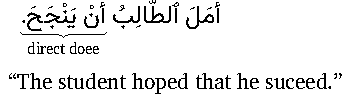
\includegraphics{A-Learners-Grammar-of-Classical-Standard-Arabic_files/figure-latex/unnamed-chunk-25-1.pdf}

We show other examples below where the
\foreignlanguage{arabic}{أَنْ} clause
occurs in place of other noun positions.

As the subject:

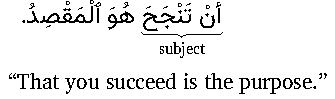
\includegraphics{A-Learners-Grammar-of-Classical-Standard-Arabic_files/figure-latex/unnamed-chunk-26-1.pdf}

As the information:

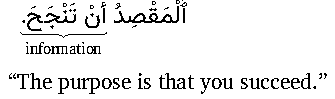
\includegraphics{A-Learners-Grammar-of-Classical-Standard-Arabic_files/figure-latex/unnamed-chunk-27-1.pdf}

As a doer noun:

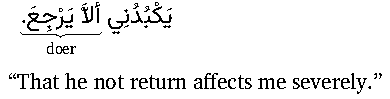
\includegraphics{A-Learners-Grammar-of-Classical-Standard-Arabic_files/figure-latex/unnamed-chunk-28-1.pdf}

In the i-state as the base noun in an annexation:

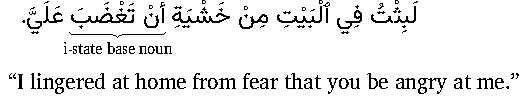
\includegraphics{A-Learners-Grammar-of-Classical-Standard-Arabic_files/figure-latex/unnamed-chunk-29-1.pdf}

In the i-state after a preposition:

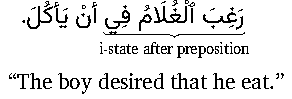
\includegraphics{A-Learners-Grammar-of-Classical-Standard-Arabic_files/figure-latex/unnamed-chunk-30-1.pdf}

\subsection{\texorpdfstring{Option to drop the preposition before \foreignlanguage{arabic}{أَنْ}}{Option to drop the preposition before أَنْ}}\label{option-to-drop-the-preposition-before-ux623ux646}

In the above example the verb \foreignlanguage{arabic}{رَغِبَ يَرْغَبُ} takes an indirect doee after the preposition \foreignlanguage{arabic}{فِي}.
In such cases, where the
\foreignlanguage{arabic}{أَنْ} clause
occurs after a preposition, it is common to drop the preposition as long as there is not resulting confusion in meaning.
So, we can also say (without the preposition \foreignlanguage{arabic}{فِي}) for the same meaning:

\foreignlanguage{arabic}{رَغِبَ ٱلْغُلَامُ آَنْ يَأْکُلَ.}\\
\enquote{The boy desired that he eat.}

\subsection{\texorpdfstring{Uncommon usages of \foreignlanguage{arabic}{أَنْ}}{Uncommon usages of أَنْ}}\label{uncommon-usages-of-ux623ux646}

Ocassionally, \foreignlanguage{arabic}{أَنْ} is used with the meaning \enquote{lest}. For example:

\foreignlanguage{arabic}{قَتَلْتُ ٱلثُّعْبَانَ أَنْ يَقْتُلَنِي.}\\
\enquote{I killed the serpent lest it kill me.}

\foreignlanguage{arabic}{أَنْ} may also occur before a completed-action verb. Example:

\foreignlanguage{arabic}{بَلَغَنِي أَنْ رَجَعْتَ.}\\
\enquote{That you have returned has reached me.}

\subsection{\texorpdfstring{Other types of \foreignlanguage{arabic}{أَنْ}}{Other types of أَنْ}}\label{other-types-of-ux623ux646}

There are other types of \foreignlanguage{arabic}{أَنْ} in the Arabic language. They all have the basic meaning \enquote{that}. But they are used in different grammatical ways.

The \foreignlanguage{arabic}{أَنْ} we have learned here is called the \emph{verbal noun \foreignlanguage{arabic}{أَنْ}} because of the equivalence of its clause with a doing verbal noun.

There is also another type of \foreignlanguage{arabic}{أَنْ} called the \emph{lightened \foreignlanguage{arabic}{أَنْ}} that we will learn in section~\ref{lightened-an}.

There is also the \emph{explanatory \foreignlanguage{arabic}{أَنْ}} and the \emph{extra \foreignlanguage{arabic}{أَنْ}} that we will cover in chapter~\ref{types-of-an}.

\section{\texorpdfstring{After \foreignlanguage{arabic}{لِ} \emph{li}}{After لِ li}}\label{after-ux644-li}

\subsection{\texorpdfstring{The \foreignlanguage{arabic}{لِ} of purpose}{The لِ of purpose}}\label{the-ux644-of-purpose}

The article \foreignlanguage{arabic}{أَنْ} may be attached to the preposition \foreignlanguage{arabic}{لِ} \emph{li} thus: \foreignlanguage{arabic}{لِأَنْ} \emph{liʾan} to give the purpose of the following verb. This \foreignlanguage{arabic}{لِ} may be translated as \enquote{so that}. For example:

\foreignlanguage{arabic}{أَکَلَ لِأَنْ يَشْبَعَ.}\\
\enquote{He ate so that he be sated.}

When \foreignlanguage{arabic}{لِ} is thus used, \foreignlanguage{arabic}{أَنْ} is optionally allowed to be dropped while its meaning is retained.
\foreignlanguage{arabic}{لِ} is then attached to the verb.
So we can say, for the same meaning:

\foreignlanguage{arabic}{أَکَلَ لِيَشْبَعَ.}\\
\enquote{He ate so that he be sated.}

But when using \foreignlanguage{arabic}{لَا} to negate the verb, then \foreignlanguage{arabic}{أَنْ} must be expressed, and the combination of \foreignlanguage{arabic}{لِ}, \foreignlanguage{arabic}{أَنْ}, and \foreignlanguage{arabic}{لَا} is written as \foreignlanguage{arabic}{لِئَلَّا} \emph{liʾallā}. For example,

\foreignlanguage{arabic}{شَرِبَ ٱلْمَاءَ لِئَلَّا يَعْطَشَ.}\\
\enquote{He drank the water so that he not be thirsty.}

By the way, the grammatical equivalence of \foreignlanguage{arabic}{أَنْ} and a following a-state incomplete-action verb with a verbal noun of doing applies also to when \foreignlanguage{arabic}{لِ} is used before (either an expressed or an implied) \foreignlanguage{arabic}{أَنْ}. So, for example, if we have a sentence:

\foreignlanguage{arabic}{قَرَأَ ٱلْکِتَابَ لِيَعْلَمَ مَفْهُومَهُ.} or\\
\foreignlanguage{arabic}{قَرَأَ ٱلْکِتَابَ لِأَنْ يَعْلَمَ مَفْهُومَهُ.}\\
\enquote{He read the book so that he know its meaning.}

Then, grammatically, \foreignlanguage{arabic}{أَنْ} and what follows it may be expressed with the verbal noun of doing \foreignlanguage{arabic}{عِلْم} thus:

\foreignlanguage{arabic}{قَرَأَ ٱلْکِتَابَ لِعِلْمِ مَفْهُومِهِ.}\\
\enquote{He read the book for the knowledge of its meaning.}

\subsection{\texorpdfstring{The \foreignlanguage{arabic}{لِ} of denial}{The لِ of denial}}\label{the-ux644-of-denial}

There is a specific \foreignlanguage{arabic}{لِ}, called the \foreignlanguage{arabic}{لِ} of denial, which is used with a-state incomplete-action verbs and the verb \foreignlanguage{arabic}{کَانَ} that we will discuss in section (TODO in \foreignlanguage{arabic}{کَانَ} chapter).

\section{\texorpdfstring{After \foreignlanguage{arabic}{کَيْ} \emph{kay}}{After کَيْ kay}}\label{after-ux643ux64a-kay}

\foreignlanguage{arabic}{کَيْ} \emph{kay}
is a preposition similar to \foreignlanguage{arabic}{لِ} in meaning. It may be translated as \enquote{in order that}, or also as \enquote{so that}.
It is also used before the a-state incomplete-action verb.
The difference from \foreignlanguage{arabic}{لِ} is that, when \foreignlanguage{arabic}{لِ} is used with the a-state incomplete-action verb, expressing or dropping the \foreignlanguage{arabic}{أَنْ} was optional.
But with \foreignlanguage{arabic}{کَيْ}, dropping the \foreignlanguage{arabic}{أَنْ} is mandatory, while its meaning is retained. For example:

\foreignlanguage{arabic}{أَکَلَ کَيْ يَشْبَعَ.}\\
\enquote{He ate in order that he be sated.}

\foreignlanguage{arabic}{لَا} is used, as usual, to negate the verb and is attached to \foreignlanguage{arabic}{کَيْ} thus: \foreignlanguage{arabic}{کَيْلَا} \emph{kaylā}. Example:

\foreignlanguage{arabic}{شَرِبَ ٱلْمَاءَ کَيْلَا يَعْطَشَ.}\\
\enquote{He drank the water in order that he not be thirsty.}

The preposition \foreignlanguage{arabic}{لِ} may be combined with \foreignlanguage{arabic}{کَيْ} thus: \foreignlanguage{arabic}{لِکَيْ} \emph{likay}, for more or less the same meaning. For example:

\foreignlanguage{arabic}{أَکَلَ لِکَيْ يَشْبَعَ.}\\
\enquote{He ate in order that he be sated.}

With \foreignlanguage{arabic}{لَا} the whole combination is written as \foreignlanguage{arabic}{لِکَيْلَا} \emph{likaylā}. \foreignlanguage{arabic}{أَنْ} must again be not be expressed.

Example:

\foreignlanguage{arabic}{شَرِبَ ٱلْمَاءَ لِکَيْلَا يَعْطَشَ.}\\
\enquote{He drank the water in order that he not be thirsty.}

By the way,
\foreignlanguage{arabic}{کَيْ} and a following a-state incomplete-action verb are not \emph{directly} replaced by
a verbal noun of doing.
So, for example, if we have a sentence:

\foreignlanguage{arabic}{قَرَأَ ٱلْکِتَابَ کَيْ يَعْلَمَ مَفْهُومَهُ.}\\
\enquote{He read the book in order that he know its meaning.}

Then \foreignlanguage{arabic}{لِ} is to be used in place of \foreignlanguage{arabic}{کَيْ} if we wish to replace it and what follows with the verbal noun of doing \foreignlanguage{arabic}{عِلْم} thus:

\foreignlanguage{arabic}{قَرَأَ ٱلْکِتَابَ لِعِلْمِ مَفْهُومِهِ.}\\
\enquote{He read the book for the knowledge of its meaning.}

\section{\texorpdfstring{After \foreignlanguage{arabic}{حَتَّىٰ} \emph{ḥattā}}{After حَتَّىٰ ḥattā}}\label{after-ux62dux62aux649-hatta}

\foreignlanguage{arabic}{حَتَّىٰ} \emph{ḥattā}
is a particle that can be used in multiple ways.
Its basic meaning is \enquote{until} or \enquote{to the point of} or \enquote{even} where it indicates an extreme limit.

Before we discuss its use with a verb following it, we will take a short digression to discuss its use with a following noun.

\subsection{\texorpdfstring{\foreignlanguage{arabic}{حَتَّىٰ} \emph{ḥattā} with a following noun}{حَتَّىٰ ḥattā with a following noun}}\label{ux62dux62aux649-hatta-with-a-following-noun}

Consider the following sentence:

\foreignlanguage{arabic}{أَکَلْتُ ٱلسَّمَکَةَ حَتَّىٰ رَأْسِهَا.}\\
\enquote{I ate the fish until its head.}

\foreignlanguage{arabic}{حَتَّىٰ} \enquote{until},
here, is used as a preposition.
Therefore,
\foreignlanguage{arabic}{رَأْس}
is in the i-state, as the noun following a preposition.
The meaning of the sentence is that the fish was eaten all the way to its head.
(Whether the head itself was eaten or not is ambiguous. The sentence itself admits both meanings.)

Consider now a variant of this sentence:

\foreignlanguage{arabic}{أَکَلْتُ ٱلسَّمَکَةَ حَتَّىٰ رَأْسَهَا.}\\
\enquote{I ate the fish, even its head.}

\foreignlanguage{arabic}{رَأْس},
here, is in the a-state because it is a direct doee of the verb \foreignlanguage{arabic}{أَکَلَ} \enquote{ate}.
The particle
\foreignlanguage{arabic}{حَتَّىٰ} \enquote{even},
here, is only a connector between the direct doees in much the same way as \foreignlanguage{arabic}{وَ} \enquote{and}.
(\foreignlanguage{arabic}{أَکَلْتُ ٱلسَّمَکَةَ وَرَأْسَهَا.}
\enquote{I ate the fish and its head.})

Consider now yet another variant of this sentence:

\foreignlanguage{arabic}{أَکَلْتُ ٱلسَّمَکَةَ. حَتَّىٰ رَأْسُهَا {[}أَکَلْتُهَا{]}.}\\
\enquote{I ate the fish. Even its head {[}I ate{]}.}

Now
\foreignlanguage{arabic}{رَأْس}
is in the u-state because it is actually the subject of a new sentence, whose information is (an either expressed or implied) \foreignlanguage{arabic}{أَکَلْتُهَا} \enquote{I ate it}.
\foreignlanguage{arabic}{حَتَّىٰ},
here, serves as an introductory particle to the second subject and does not affect the state of the following noun.

\subsection{\texorpdfstring{\foreignlanguage{arabic}{حَتَّىٰ} \emph{ḥattā} with a following verb}{حَتَّىٰ ḥattā with a following verb}}\label{ux62dux62aux649-hatta-with-a-following-verb}

Just as
\foreignlanguage{arabic}{حَتَّىٰ}
is used for different purposes with a following noun,
so too is it used with different purposes with a verb following it.

\subsubsection{\texorpdfstring{\foreignlanguage{arabic}{حَتَّىٰ} with a following a-state incomplete-action verb}{حَتَّىٰ with a following a-state incomplete-action verb}}\label{ux62dux62aux649-with-a-following-a-state-incomplete-action-verb}

When
\foreignlanguage{arabic}{حَتَّىٰ}
is used with an expectation or purpose of a future action of the verb following it, then
the verb following it is an a-state incomplete-action verb.
This is done in the following two scenarios:

\begin{enumerate}
\def\labelenumi{\arabic{enumi}.}
\item
  When \foreignlanguage{arabic}{حَتَّىٰ} is used to indicate an extreme point at which the action of the following verb would occur, or is meant to occur. Here,
  \foreignlanguage{arabic}{حَتَّىٰ}
  may be translated as \enquote{to the point of} and the verb following it is translated using \enquote{-ing}.
  For example,

  \foreignlanguage{arabic}{قَرَأْتُ ٱلْقُرْآنَ حَتَّىٰ أَخْتِمَهُ.}\\
  \enquote{I read the Qurʾān to the point of finishing it.}

  \foreignlanguage{arabic}{يَغْضَبُ حَتَّىٰ يَهْرَبُوا مِنْهُ.}\\
  \enquote{He becomes angry to the point of their fleeing from him.}

  \foreignlanguage{arabic}{غَضِبَ حَتَّىٰ لَا يَمْلِکَ نَفْسَهُ.}\\
  \enquote{He became angry to the point of not controlling himself.}

  It is noteworthy that the use of \foreignlanguage{arabic}{حَتَّىٰ}, here, implies only that the following action is meant to occur, or is at the point of being expected to occur. It doesn't actually state that the action will actually occur, for something may prevent it from occurring in reality.

  Note, also, that \foreignlanguage{arabic}{لَا} is not attached to \foreignlanguage{arabic}{حَتَّىٰ} in \foreignlanguage{arabic}{حَتَّىٰ لَا}.

  Also, similar to the case of \foreignlanguage{arabic}{کَيْ}, there is an assumed (but mandatorily unexpressed) \foreignlanguage{arabic}{أَنْ} which is the real cause of the following incomplete-action verb being in the a-state.
  In fact,
  \foreignlanguage{arabic}{حَتَّىٰ},
  here, can be considered synonymous to \foreignlanguage{arabic}{إِلَىٰ أَنْ} \enquote{to {[}the point{]} that}. So the above examples can be considered similar in meaning to:

  \foreignlanguage{arabic}{قَرَأْتُ ٱلْقُرْآنَ إِلَىٰ أَنْ أَخْتِمَهُ.}

  \foreignlanguage{arabic}{يَغْضَبُ إِلَىٰ أَنْ يَهْرَبُوا مِنْهُ.}

  \foreignlanguage{arabic}{غَضِبَ إِلَىٰ أَلَّا يَمْلِکَ نَفْسَهُ.}
\item
  When \foreignlanguage{arabic}{حَتَّىٰ} is used with the meaning \enquote{to such a purpose that}. This is a similar meaning to \foreignlanguage{arabic}{کَيْ} \enquote{in order that}.
  For example,

  \foreignlanguage{arabic}{أَذْهَبُ إِلَيْهِ حَتَّىٰ يَأْمُرَنِي بِشَيْءٍ.}\\
  \enquote{I go to him to such a purpose that he order me {[}to do{]} something.}

  \foreignlanguage{arabic}{وَعَظَ ٱلْأَبُ ٱبْنَهُ حَتَّىٰ يَصْلُحَ.}\\
  \enquote{The father admonished his son to such a purpose that he be righteous.}

  Again, there is an assumed (but mandatorily unexpressed) \foreignlanguage{arabic}{أَنْ} which is the real cause of the following incomplete-action verb being in the a-state.
\end{enumerate}

Sometimes, the sentence itself may admit both of the above meanings. For example:

\foreignlanguage{arabic}{يَأْکُلُ حَتَّىٰ يَشْبَعَ.}\\
\enquote{He eats to the point of being full.}\\
and/or\\
\enquote{He eats to the purpose that he be full.}

Context would be needed to determine which meaning or whether both meanings are intended.

\subsubsection{\texorpdfstring{\foreignlanguage{arabic}{حَتَّىٰ} with no effect on the following verb}{حَتَّىٰ with no effect on the following verb}}\label{ux62dux62aux649-with-no-effect-on-the-following-verb}

If
\foreignlanguage{arabic}{حَتَّىٰ}
is not used with any expectation or purpose of a future action of the verb following it, then it has no effect on this verb.
(It goes without saying that an implicit \foreignlanguage{arabic}{أَنْ} is not assumed with \foreignlanguage{arabic}{حَتَّىٰ} in this case.)

The verb following
\foreignlanguage{arabic}{حَتَّىٰ}
in this case
may even be a completed-action verb. For example:

\foreignlanguage{arabic}{أَکَلْتُ ٱلطَّعَامَ حَتَّىٰ شَبِعْتُ.}\\
\enquote{I ate the food until I became full.}

When used with a following incomplete-action verb, the verb is put in the u-state and the meaning is that the action of the verb \emph{before}
\foreignlanguage{arabic}{حَتَّىٰ}
was done to such an extent that it caused
the action of the verb \emph{following}
\foreignlanguage{arabic}{حَتَّىٰ}
to definitely occur.
The action before
\foreignlanguage{arabic}{حَتَّىٰ}
must necessarily be a past action, and the action following
\foreignlanguage{arabic}{حَتَّىٰ}
must necessarily be a present (not a future) action.
For example,

\foreignlanguage{arabic}{أَکَلْتُ ٱلطَّعَامَ حَتَّىٰ أَشْبَعُ.}\\
\enquote{I ate the food to such an extent that I am (being) full.}

\foreignlanguage{arabic}{غَضِبَ حَتَّىٰ يَهْرَبُونَ مِنْهُ.}\\
\enquote{He became so angry that they are fleeing from him.}

\foreignlanguage{arabic}{غَضِبَ حَتَّىٰ لَا يَمْلِکُ نَفْسَهُ.}\\
\enquote{He became so angry that he is not controlling himself.}

Compare these examples with the corresponding ones in the previous sub-section that have an a-state incomplete action verb.

\section{\texorpdfstring{After \foreignlanguage{arabic}{لَنْ} \emph{lan}}{After لَنْ lan}}\label{after-ux644ux646-lan}

\foreignlanguage{arabic}{لَا} and \foreignlanguage{arabic}{أَنْ} are combined to form \foreignlanguage{arabic}{لَنْ} \emph{lan} with the meaning \enquote{shall not}. \foreignlanguage{arabic}{لَنْ} is used with the a-state incomplete-action verb to emphatically negate the future.

\foreignlanguage{arabic}{لَنْ تَذْهَبَ.}\\
\enquote{You\textsubscript{1m} shall not go.}

\section{\texorpdfstring{After \foreignlanguage{arabic}{إِذَنْ} \emph{ʾid͡han}}{After إِذَنْ ʾid͡han}}\label{after-ux625ux630ux646-eipan}

TODO

\section{\texorpdfstring{After \foreignlanguage{arabic}{وَ}, \foreignlanguage{arabic}{فَ}, \foreignlanguage{arabic}{أَوْ}, and \foreignlanguage{arabic}{ثُمَّ}}{After وَ, فَ, أَوْ, and ثُمَّ}}\label{after-ux648-ux641-ux623ux648-and-ux62bux645}

\subsection{As connectors}\label{as-connectors}

If the connectors
\foreignlanguage{arabic}{وَ}, \foreignlanguage{arabic}{فَ}, \foreignlanguage{arabic}{أَوْ}, and \foreignlanguage{arabic}{ثُمَّ}
occur after an a-state incomplete-action verb, then
a second a-state incomplete-action verb
(that doesn't have its own \foreignlanguage{arabic}{أَنْ}, etc.)
may be either in the a-state or the u-state.
For example,

\foreignlanguage{arabic}{أَرْغَبُ أَنْ أَحْضُرَ ٱلْمَجْلِسَ وَأَسْمَعَ.} (\foreignlanguage{arabic}{أَسْمَعَ} in a-state)\\
\enquote{I desire that I attend the session and {[}that{]} I listen.}

or

\foreignlanguage{arabic}{أَرْغَبُ أَنْ أَحْضُرَ ٱلْمَجْلِسَ وَأَسْمَعُ.} (\foreignlanguage{arabic}{أَسْمَعَ} in u-state)\\
\enquote{I desire that I attend the session and I will listen.}

\subsection{With special meanings}\label{with-special-meanings}

\foreignlanguage{arabic}{وَ}, \foreignlanguage{arabic}{فَ}, \foreignlanguage{arabic}{أَوْ}, and \foreignlanguage{arabic}{ثُمَّ} also cause the following incomplete-action verb to be in the a-state in their own right, not simply as connectors. This is discussed in more detail in chapter TODO.

\chapter{ø-state incomplete-action verbs}\label{state-incomplete-action-verbs}

\section{Introduction}\label{introduction-18}

In
chapter~\ref{u-state-incomplete-action-verbs}
we mentioned that incomplete action verbs have three states (like nouns).
These states are called:

\begin{enumerate}
\def\labelenumi{\roman{enumi}.}
\tightlist
\item
  The u-state
\item
  The a-state
\item
  The ø-state
\end{enumerate}

We have already studied the u-state of incomplete-action verbs in
chapter~\ref{u-state-incomplete-action-verbs}.
And we will defer the study of
a-state of incomplete-action verbs to
chapter~\ref{a-state-incomplete-action-verbs}.
In this chapter we will study the
ø-state
incomplete-action verb.

We will also study the \emph{verb of command} which is very similar to the
ø-state
incomplete-action verb.

\section{Forming the ø-state incomplete-action verb}\label{forming-the-0-state-incomplete-action-verb}

Here is the u-state incomplete action verb for the singular masculine absentee participant doer \enquote{he}:

\foreignlanguage{arabic}{يَفْعَلُ}\\
\emph{yafɛalu}\\
\enquote{he does}

Note that, because it is in the u-state, the its final letter ends with a \emph{u}-mark \foreignlanguage{arabic}{◌ُ}.
In order to form the
ø-state
incomplete-action verb,
we change the \emph{u}-mark into a
ø-mark \foreignlanguage{arabic}{◌ْ}, thus:

\foreignlanguage{arabic}{يَفْعَلْ}\\
\emph{yafɛal}

This is done for all participants whose doer pronoun is invisible and u-state verb ends with a \emph{u}-mark \foreignlanguage{arabic}{◌ُ}.

For participants whose doer pronoun is followed by an extra \foreignlanguage{arabic}{ن} in the u-state verb, this final \foreignlanguage{arabic}{ن} is dropped in order to form the
ø-state
incomplete-action verb.
So, for example, the u-state
incomplete-action verb:

\foreignlanguage{arabic}{يَفْعَلَانِ}\\
\emph{yafɛalāni}\\
\enquote{they\textsubscript{2,m} do}

becomes, for the
ø-state:

\foreignlanguage{arabic}{يَفْعَلَا}\\
\emph{yafɛalā}

Here is the complete table of the
ø-state
incomplete-action verb
for all doer participants.

\begin{longtable}[]{@{}
  >{\raggedright\arraybackslash}p{(\columnwidth - 6\tabcolsep) * \real{0.2667}}
  >{\raggedright\arraybackslash}p{(\columnwidth - 6\tabcolsep) * \real{0.2000}}
  >{\raggedright\arraybackslash}p{(\columnwidth - 6\tabcolsep) * \real{0.2667}}
  >{\raggedright\arraybackslash}p{(\columnwidth - 6\tabcolsep) * \real{0.2667}}@{}}
\toprule\noalign{}
\begin{minipage}[b]{\linewidth}\raggedright
Participant
\end{minipage} & \begin{minipage}[b]{\linewidth}\raggedright
Incomplete-action verb doer pronoun
\end{minipage} & \begin{minipage}[b]{\linewidth}\raggedright
u-state incomplete-action verb
\end{minipage} & \begin{minipage}[b]{\linewidth}\raggedright
ø-state incomplete-action verb
\end{minipage} \\
\midrule\noalign{}
\endhead
\bottomrule\noalign{}
\endlastfoot
he & \emph{invisible} & \foreignlanguage{arabic}{يَفْعَلُ} & \foreignlanguage{arabic}{يَفْعَلْ} \\
she & \emph{invisible} & \foreignlanguage{arabic}{تَفْعَلُ} & \foreignlanguage{arabic}{تَفْعَلْ} \\
you\textsubscript{1,m} & \emph{invisible} & \foreignlanguage{arabic}{تَفْعَلُ} & \foreignlanguage{arabic}{تَفْعَلْ} \\
you\textsubscript{1,f} & \foreignlanguage{arabic}{ي} & \foreignlanguage{arabic}{تَفْعَلِينَ} & \foreignlanguage{arabic}{تَفْعَلِي} \\
I & \emph{invisible} & \foreignlanguage{arabic}{أَفْعَلُ} & \foreignlanguage{arabic}{أَفْعَلْ} \\
they\textsubscript{2,m} & \foreignlanguage{arabic}{ا} & \foreignlanguage{arabic}{يَفْعَلَانِ} & \foreignlanguage{arabic}{يَفْعَلَا} \\
they\textsubscript{2,f} & \foreignlanguage{arabic}{ا} & \foreignlanguage{arabic}{تَفْعَلَانِ} & \foreignlanguage{arabic}{تَفْعَلَا} \\
you\textsubscript{2} & \foreignlanguage{arabic}{ا} & \foreignlanguage{arabic}{تَفْعَلَانِ} & \foreignlanguage{arabic}{تَفْعَلَا} \\
they\textsubscript{3+,m} & \foreignlanguage{arabic}{و} & \foreignlanguage{arabic}{يَفْعَلُونَ} & \foreignlanguage{arabic}{يَفْعَلُوا} \\
they\textsubscript{3+,f} & \foreignlanguage{arabic}{نَ} & \foreignlanguage{arabic}{يَفْعَلْنَ} & \foreignlanguage{arabic}{يَفْعَلْنَ} (same) \\
you\textsubscript{3+,m} & \foreignlanguage{arabic}{و} & \foreignlanguage{arabic}{تَفْعَلُونَ} & \foreignlanguage{arabic}{تَفْعَلُوا} \\
you\textsubscript{3+,f} & \foreignlanguage{arabic}{نَ} & \foreignlanguage{arabic}{تَفْعَلْنَ} & \foreignlanguage{arabic}{تَفْعَلْنَ} (same) \\
we & \emph{invisible} & \foreignlanguage{arabic}{نَفْعَلُ} & \foreignlanguage{arabic}{نَفْعَلْ} \\
\end{longtable}

Take note the following:

\begin{itemize}
\tightlist
\item
  The u-state and ø-state verbs are the same for the feminine plural absentee and addressee participants:

  \begin{itemize}
  \tightlist
  \item
    \foreignlanguage{arabic}{يَفْعَلْنَ} (they\textsubscript{3+,f})
  \item
    \foreignlanguage{arabic}{تَفْعَلْنَ} (you\textsubscript{3+,f})
  \end{itemize}
\item
  The u-state and ø-state verbs for the masculine plural absentee and addressee participants have a final silent \foreignlanguage{arabic}{أَلِف}:

  \begin{itemize}
  \tightlist
  \item
    \foreignlanguage{arabic}{يَفْعَلُوا} (they\textsubscript{3+,m})
  \item
    \foreignlanguage{arabic}{تَفْعَلُوا} (you\textsubscript{3+,m})
  \end{itemize}
\item
  When the
  ø-state
  incomplete-action verb
  ends with a
  ø-mark \foreignlanguage{arabic}{◌ْ}, and the next word begins with a connecting hamzah \foreignlanguage{arabic}{ٱ} then the
  ø-mark \foreignlanguage{arabic}{◌ْ} is converted to an \emph{i} mark \foreignlanguage{arabic}{◌ِ}. For example:

  \begin{itemize}
  \tightlist
  \item
    \foreignlanguage{arabic}{يَفْعَلْ + ٱلرَّجُلُ = يَفْعَلِ ٱلرَّجُلُ}
  \end{itemize}
\end{itemize}

\section{\texorpdfstring{With \foreignlanguage{arabic}{لِ} for indirect commands}{With لِ for indirect commands}}\label{indirect-commands}

The particle \foreignlanguage{arabic}{لِ} when connected to the front of a
incomplete-action verb
causes it to be in the
ø-state
and gives it the meaning of an indirect command. In English this can be translated using \enquote{should} or \enquote{let}:

\foreignlanguage{arabic}{لِيَذْهَبِ ٱَلرَّجُلُ}\\
\enquote{The man should go!}\\
or\\
\enquote{Let the man go!}\\
(\enquote{Let} is being used here as a command for the man, not for the addressee of this speech.)

\foreignlanguage{arabic}{لِنَذْهَبْ!}\\
\enquote{Let's go!}

The indirect command is only rarely used for the addressee participant. Instead, the verb of command is used which we will study in section~\ref{verb-of-command} later in this chapter.

The particles \foreignlanguage{arabic}{فَ} \enquote{so} and \foreignlanguage{arabic}{وَ} \enquote{and} are frequently used before this \foreignlanguage{arabic}{لِ}.
The \foreignlanguage{arabic}{لِ} then loses its \emph{i}-mark and gets a
ø-mark. Examples:

\foreignlanguage{arabic}{فَلْنَأْکُلْ طَعَامَنَا وَلْنَشْرَبْ شَرَابَنَا.}\\
\enquote{So let us eat our food and drink our drink!}

\foreignlanguage{arabic}{لِتَجْلِسُوا عَلَى ٱلْأَرْضِ.}\\
\enquote{You should sit on the ground!}

\section{\texorpdfstring{With \foreignlanguage{arabic}{لَا} for prohibitions}{With لَا for prohibitions}}\label{la-of-prohibition}

The word \foreignlanguage{arabic}{لَا} when in front of a
ø-state
incomplete-action verb
gives the meaning of a prohibition.
In English this can be translated using \enquote{Don't}.

For example,

\foreignlanguage{arabic}{لَا تَکْتُبُوا}\\
\enquote{Don't write\textsubscript{3,m}!}

\foreignlanguage{arabic}{يَا زَيْدُ، لَا تَدْخُلِ ٱلْبَيْتَ!}\\
\enquote{Don't\textsubscript{1,m} enter the house!}

The particles \foreignlanguage{arabic}{فَ} \enquote{so} and \foreignlanguage{arabic}{وَ} \enquote{and} may be used before this \foreignlanguage{arabic}{لَا}.
Example:

\foreignlanguage{arabic}{فَلَا تَأْکُلْ وَلَا تَشْرَبْ!}\\
\enquote{So don't eat\textsubscript{1,m} and don't drink\textsubscript{1,m}!}

Such prohibitions are generally for the addressee participant.
However, rarely, they may be issued for the absentee participant as well. Example:

\foreignlanguage{arabic}{لَايَمْنَعْ زَيْدًا ٱلدُّخُولَ.}\\
\enquote{Let him not prevent Zayd from entering!}

By the way, \foreignlanguage{arabic}{لَا} does not force a verb to be in the u-state
ø-state. We have already seen in
section~\ref{u-state-verb-negation-la}
that \foreignlanguage{arabic}{لَا} can be used to negate a u-state incomplete-action verb for the present and future tense.
Example:

\foreignlanguage{arabic}{لَا يَذْهَبُ ٱلرَّجُلُ}\\
\emph{lā yad͡h·habu -rrajulu.}\\
\enquote{The man does not go.} or,\\
\enquote{The man is not going.} or,\\
\enquote{The man will not go.}

\section{\texorpdfstring{With \foreignlanguage{arabic}{لَمْ} for \enquote{did not}}{With لَمْ for ``did not''}}\label{with-ux644ux645-for-did-not}

The particle \foreignlanguage{arabic}{لَمْ} when in front of an
incomplete-action verb
causes it to be in the
ø-state
and gives it the meaning of
negating the past tense
In English this can be translated using \enquote{did not}.
For example,

\foreignlanguage{arabic}{لَمْ يَذْهَبِ ٱلرَّجُلُ.}\\
\enquote{The man did not go.}

We have already learned in
section~\ref{negating-completed-action-verbs} that the completed-action verb is negated using the particle \foreignlanguage{arabic}{مَا}. For example:

\foreignlanguage{arabic}{مَا ذَهَبَ ٱلرَّجُلُ.}\\
\emph{mā d͡hahaba -rrajulu.}\\
\enquote{The man did not go.}\\
or,\\
\enquote{The man has not gone.}

Both \foreignlanguage{arabic}{لَمْ} and \foreignlanguage{arabic}{مَا} are used commonly to negate the past tense.
\foreignlanguage{arabic}{مَا} has a more emphatic meaning than \foreignlanguage{arabic}{لَمْ}.

Here are some more examples:

\section{\texorpdfstring{With \foreignlanguage{arabic}{لَمَّا} for \enquote{did not yet}}{With لَمَّا for ``did not yet''}}\label{with-ux644ux645ux627-for-did-not-yet}

The word \foreignlanguage{arabic}{لَمَّا} when in front of a
ø-state
incomplete-action verb
gives the meaning \enquote{did not yet}.
For example,

\foreignlanguage{arabic}{لَمَّا يَذْهَبْ زَيْدٌ.}\\
\enquote{Zayd did not go yet.}

\section{Other uses of the ø-state incomplete-action verb}\label{other-uses-of-the-0-state-incomplete-action-verb}

The ø-state incomplete-action verb is also used for \emph{consequential actions} and in \emph{conditional statements}. We will deal with these in
chapters~\ref{the-consequential-action}
and~\ref{conditional-statements}
respectively

\section{The verb of command}\label{verb-of-command}

In order to give a direct command to an addressee, Arabic uses the verb of command. The verb of command is very similar to the
ø-state
incomplete-action verb.
The verb of command is only available for the addressee participant.

\subsection{Forming the verb of command}\label{forming-the-verb-of-command}

Here is the verb of command for the addressee participants:

\begin{longtable}[]{@{}ll@{}}
\toprule\noalign{}
Participant & Verb of command \\
\midrule\noalign{}
\endhead
\bottomrule\noalign{}
\endlastfoot
you\textsubscript{1,m} & \foreignlanguage{arabic}{ٱفْعَلْ} \\
you\textsubscript{1,f} & \foreignlanguage{arabic}{ٱفْعَلِي} \\
you\textsubscript{2} & \foreignlanguage{arabic}{ٱفْعَلَا} \\
you\textsubscript{3+,m} & \foreignlanguage{arabic}{ٱفْعَلُوا} \\
you\textsubscript{3+,f} & \foreignlanguage{arabic}{ٱفْعَلْنَ} \\
\end{longtable}

In order to form the verb of command, we remove the initial \foreignlanguage{arabic}{ت} from the addressee particpant verb. The verb then begins with an ø-mark so we place a connecting hamzah in front of it.

When the verb of command occurs in the beginning of a sentence, then the vowel mark for the connecting hamzah is selected according to the following criteria:

\begin{enumerate}
\def\labelenumi{\roman{enumi}.}
\item
  When the middle root letter of the verb of command has an \emph{u}-mark~\foreignlanguage{arabic}{◌ُ}, then the connecting hamzah gets an \emph{u}-mark~too. Examples:

  \begin{longtable}[]{@{}ll@{}}
  \toprule\noalign{}
  Verb & Verb of command for \enquote{he} \\
  \midrule\noalign{}
  \endhead
  \bottomrule\noalign{}
  \endlastfoot
  \foreignlanguage{arabic}{نَظَرَ يَنْظُرُ نَظَرًا} & \foreignlanguage{arabic}{ٱُنْظُرْ} \enquote{Look!} \\
  \foreignlanguage{arabic}{قَتَلَ يَقْتُلُ قَتْلًا} & \foreignlanguage{arabic}{ٱُقْتُلْ} \enquote{Kill!} \\
  \foreignlanguage{arabic}{مَکَثَ يَمْکُثُ مُکُوثًا} & \foreignlanguage{arabic}{ٱُمْکُثْ} \enquote{Stay!} \\
  \end{longtable}
\item
  Otherwise, when the middle root letter of the verb of command has an \emph{a}-mark~\foreignlanguage{arabic}{◌َ} or an \emph{i}-mark~\foreignlanguage{arabic}{◌ِ}, then the connecting hamzah gets an \emph{i}-mark~\foreignlanguage{arabic}{◌ِ}. Examples:

  \begin{longtable}[]{@{}ll@{}}
  \toprule\noalign{}
  Verb & Verb of command for \enquote{he} \\
  \midrule\noalign{}
  \endhead
  \bottomrule\noalign{}
  \endlastfoot
  \foreignlanguage{arabic}{عَمِلَ يَعْمَلُ عَمَلًا} & \foreignlanguage{arabic}{ٱِعْمَلْ} \enquote{Work!} \\
  \foreignlanguage{arabic}{ذَهَبَ يَذْهَبُ ذَهَابًا} & \foreignlanguage{arabic}{ٱِذْهَبْ} \enquote{Go!} \\
  \foreignlanguage{arabic}{جَلَسَ يَجْلِسُ جُلُوسًا} & \foreignlanguage{arabic}{ٱِجْلِسْ} \enquote{Sit!} \\
  \end{longtable}
\end{enumerate}

Here are some examples of using the verb of command:

The verb of command is not used to issue negative commands, like \enquote{Don't go!}.
Instead, the
ø-state verb is used with \foreignlanguage{arabic}{لَا}
as described in
section~\ref{la-of-prohibition}
above.

\foreignlanguage{arabic}{لَا تَذْهَبْ}\\
\enquote{Don't go!}

\subsection{The verb of command for roots begin with hamzah}\label{the-verb-of-command-for-roots-begin-with-hamzah}

Appendix~\ref{hamzarules} details the rules for speeling words that contain hamzah generally.
In addition to those rules, the verb of command for roots that begin with hamzah warrant additional discussion.

Consider the following form~1 verbs and their verbs of command
for the singular masculine addressee doer \enquote{he}:

\begin{longtable}[]{@{}
  >{\raggedright\arraybackslash}p{(\columnwidth - 4\tabcolsep) * \real{0.1818}}
  >{\raggedright\arraybackslash}p{(\columnwidth - 4\tabcolsep) * \real{0.4545}}
  >{\raggedright\arraybackslash}p{(\columnwidth - 4\tabcolsep) * \real{0.3636}}@{}}
\toprule\noalign{}
\begin{minipage}[b]{\linewidth}\raggedright
Root
\end{minipage} & \begin{minipage}[b]{\linewidth}\raggedright
Verb
\end{minipage} & \begin{minipage}[b]{\linewidth}\raggedright
Verb of command
\end{minipage} \\
\midrule\noalign{}
\endhead
\bottomrule\noalign{}
\endlastfoot
\foreignlanguage{arabic}{«أمل»} & \foreignlanguage{arabic}{أَمَلَ يَأْمُلُ أَمَلًا} \enquote{to hope} & \foreignlanguage{arabic}{ٱؤْمُلْ} \\
\foreignlanguage{arabic}{«أذن»} & \foreignlanguage{arabic}{أَذِنَ يَأذَنُ أَذَنًا} \enquote{to permit} & \foreignlanguage{arabic}{ٱئْذَنْ} \\
\end{longtable}

Here are examples of these verbs of commands in the middle of a sentence:

\foreignlanguage{arabic}{يَا أُمِّي ٱئْذَنِي لِي ٱللَّعِبَ!}\\
\emph{yā ʾummi -ʾd͡hanī li -llaɛib!}\\
\enquote{O my mother, permit me to play!}

\foreignlanguage{arabic}{يَا زَيْدُ ٱؤْمُلِ ٱلْخَيْرَ!}\\
\emph{yā zaydu -ʾmuli -lk͡hayr!}\\
\enquote{O Zayd, hope for good!}

When these verbs of command occur in the beginning of the sentence, then there would be two hamzahs occuring next to each other which is not permitted. So the second hamzah is pronounced as a long vowel, though it may still be written as a hamzah. Examples:

\foreignlanguage{arabic}{ٱُؤمُلِ ٱلْخَيْرَ يَا زَيْدُ!}\\
\emph{ʾūmul}\\
not\\
\(\times\)~\emph{ʾuʾmul}

\foreignlanguage{arabic}{ٱِئذَنِي لِي ٱللَّعِبَ يَا أُمِّي!}\\
\emph{ʾīd͡hanī}\\
not\\
\(\times\)~\emph{ʾiʾd͡hanī}

As a further complication, when the verb of command is preceded by
\foreignlanguage{arabic}{وَ} \enquote{and}
or
\foreignlanguage{arabic}{فَ} \enquote{so}
then the connecting \emph{hamza} is not written
and the hamzah of the first root letter is written seated on an \foreignlanguage{arabic}{أَلِف}.
Examples:

\foreignlanguage{arabic}{وَأْمُلْ}\\
\emph{waʾmul}\\
\enquote{And hope!}

\foreignlanguage{arabic}{فَأْذَنْ}\\
\emph{faʾd͡han}\\
\enquote{So permit!}

\subsection{Irregular verbs of command}\label{irregular-verbs-of-command}

In addition to the rules states above there are four verbs of command (all containing hamzah) that are irregular. We will discuss them below:

\subsubsection{\texorpdfstring{The verbs \foreignlanguage{arabic}{أَکَلَ}~, \foreignlanguage{arabic}{أَخَذَ}~, and \foreignlanguage{arabic}{أَمَرَ}}{The verbs أَکَلَ~, أَخَذَ~, and أَمَرَ}}\label{the-verbs-ux623ux643ux644-ux623ux62eux630-and-ux623ux645ux631}

The verbs of command for the following three verbs are irregular:

\begin{longtable}[]{@{}lll@{}}
\toprule\noalign{}
Root & Verb & Verb of command \\
\midrule\noalign{}
\endhead
\bottomrule\noalign{}
\endlastfoot
\foreignlanguage{arabic}{«أکل»} & \foreignlanguage{arabic}{أَکَلَ يَأْکُلُ أَکْلًا} \enquote{to eat} & \foreignlanguage{arabic}{کُلْ} \\
\foreignlanguage{arabic}{«أخذ»} & \foreignlanguage{arabic}{أَخَذَ يَأْخُذُ أَخْذًا} \enquote{to take} & \foreignlanguage{arabic}{خُذْ} \\
\foreignlanguage{arabic}{«أمر»} & \foreignlanguage{arabic}{أَمَرَ يَأْمُرُ أَمْرًا} \enquote{to order} & \foreignlanguage{arabic}{مُرْ} \\
\end{longtable}

As you can see, the initial hamzah has been completely deleted for the verbs of command.
However, of these verbs, the verb of command for
\foreignlanguage{arabic}{أَمَرَ يَأْمُرُ أَمْرًا}
is permitted to retain its initial hamzah when preceded by
\foreignlanguage{arabic}{وَ} \enquote{and}
or
\foreignlanguage{arabic}{فَ} \enquote{so}. Then, it becomes

\foreignlanguage{arabic}{وَأْمُرْ} \emph{waʾmur}\\
and\\
\foreignlanguage{arabic}{فَأْمُرْ} \emph{faʾmur}

This retaining of the initial hamzah is not done for the other two verbs.

Here are some examples of these verbs of command:

\subsubsection{\texorpdfstring{The verb \foreignlanguage{arabic}{سَأَلَ}}{The verb سَأَلَ}}\label{the-verb-ux633ux623ux644}

The verb \foreignlanguage{arabic}{سَأَلَ يَسْأَلُ سُؤَالًا} \enquote{to question} forms its verb of command both regularly, and irregularly:

\begin{enumerate}
\def\labelenumi{\roman{enumi}.}
\tightlist
\item
  Regular: \foreignlanguage{arabic}{ٱسْأَلْ} \emph{ʾisʾal}
\item
  Irregular: \foreignlanguage{arabic}{سَلْ} \emph{sal}
\end{enumerate}

If the verb of command is preceded by
\foreignlanguage{arabic}{وَ} \enquote{and}
or
\foreignlanguage{arabic}{فَ} \enquote{so}, then the regular verb of command
\foreignlanguage{arabic}{ٱسْأَلْ} \emph{ʾisʾal} is often preferred.

Otherwise, the irregular verb of command
\foreignlanguage{arabic}{سَلْ} \emph{sal} is often preferred.

Examples of usage:

\chapter{The unknown-doer verb}\label{the-unknown-doer-verb}

\section{Introduction}\label{introduction-19}

Consider the sentence:

\foreignlanguage{arabic}{شَرِبَ زَيْدٌ ٱلْمَاءَ.}\\
\emph{s͡hariba zayduni -lmāʾ.}\\
\enquote{Zayd drank the water.}

In this sentence, \foreignlanguage{arabic}{زَيْدٌ} \enquote{Zayd} is the doer of the verb \foreignlanguage{arabic}{شَرِبَ} \enquote{drank}.
This construction of the verb, which we have been using so far, is called the \emph{known-doer verb} construction,
because the doer of the verb, in this case \enquote{Zayd} is known.
Now consider the following sentence:

\foreignlanguage{arabic}{شُرِبَ ٱلْمَاءُ.}\\
\emph{s͡huriba -lmāʾ.}\\
\enquote{The water was drunk.}

In this sentence, the doer of the verb, i.e.~the person who is doing the action of the verb \enquote{to drink}, is not mentioned.
From the sentence itself it is unknown who the doer is.
This construction of the verb is called the \emph{unknown-doer verb} construction.

\section{Forming the unknown-doer verb}\label{forming-the-unknown-doer-verb}

So far we have been studing form~1 verbs, which use only the three root letters.
As we know, the vowel on the middle root letter is variable for known-doer verbs, for example:

\begin{itemize}
\tightlist
\item
  \foreignlanguage{arabic}{شَرِبَ يَشْرَبُ} \enquote{to drink}.
\item
  \foreignlanguage{arabic}{فَتَحَ يَفْتَحُ} \enquote{to open}
\item
  \foreignlanguage{arabic}{کَبُرَ يَکْبُرُ} \enquote{to become big}
\item
  etc.
\end{itemize}

The pattern of unknown-doer verb for form 1 verbs is always:

\foreignlanguage{arabic}{فُعِلَ يُفْعَلُ}\\
\emph{fuɛila yufɛalu}

This is regardless of the vowel on the middle root letter in the known-doer verb.
If there is more than one verb from the same root, with different middle root letter vowels for the known-doer verb, then they will share the same unknown-doer verb. For example, the known-doer verbs: \foreignlanguage{arabic}{حَسَبَ يَحْسُبُ} \enquote{to reckon} and \foreignlanguage{arabic}{حَسِبَ يَحْسِبُ} \enquote{to deem} share the same unknown-doer verb: \foreignlanguage{arabic}{حُسِبَ يُحْسَبُ}.

The same doer pronouns are used for the unknown-doer verb as for the known-doer verb.
And the incomplete-action unknown-doer verb has the same three states as the incomplete-action known-doer verb.
For example:

\begin{itemize}
\tightlist
\item
  \foreignlanguage{arabic}{فُعِلُوا} \emph{fuɛilū} \enquote{they\textsubscript{3m}} (completed-action)
\item
  \foreignlanguage{arabic}{تُفْعَلَانِ} \emph{tufɛalāni} \enquote{you\textsubscript{2}} or \enquote{they\textsubscript{2f}} (u-state incomplete-action)
\item
  \foreignlanguage{arabic}{أُفْعَلَ} \emph{ʾufɛala} \enquote{I} (a-state incomplete-action)
\item
  etc.
\end{itemize}

The complete table showing the doer pronouns is given in appendix~\ref{verb-tables}.

\section{The deputy doer}\label{the-deputy-doer}

Consider again this sentence with an unknown-doer verb construction:

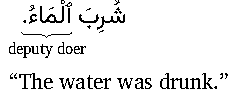
\includegraphics{A-Learners-Grammar-of-Classical-Standard-Arabic_files/figure-latex/unnamed-chunk-31-1.pdf}

Note that the noun \foreignlanguage{arabic}{ٱَلْمَاءُ} \emph{ʾalmāʾu} \enquote{the water} is in the u-state. This is because, in the absence of the doer, the direct-doee of the known-doer verb (\foreignlanguage{arabic}{ٱَلْمَاءَ}) is deputized to take doer's place in the u-state. It is then known as the \emph{deputy doer}.

The doer pronouns for the unknown-doer verb shall therefore match the gender and number of the deputy doer. Here are some examples:

\foreignlanguage{arabic}{شُکِرَتِ ٱلأُمَّهَاتُ وَمُدِحْنَ.}\\
\emph{s͡hukirati -lʾummahātu wamudiḥn.}\\
\enquote{The mothers were thanked and praised.}

\foreignlanguage{arabic}{أَنْتُمَا تُغْبَنَانِ وَتُخْدَعَانِ.}\\
\emph{ʾantumā tug͡hbanāni watuk͡hdaɛān.}\\
\enquote{You\textsubscript{2} are being cheated and deceived.}

\foreignlanguage{arabic}{مَا قُطِعَتِ ٱلشَّجَرَةُ.}\\
\emph{mā quṭiɛati -s͡hs͡hajarah.}\\
\enquote{The tree was not cut.}

\subsection{The deputy doer for multiple direct doees}\label{the-deputy-doer-for-multiple-direct-doees}

Some verbs, in the known-doer construction, take multiple doees. These verbs can be classified into two classes:

\begin{enumerate}
\def\labelenumi{\alph{enumi}.}
\item
  Verbs that cause the first direct doee to be affected by, or asked for, the second direct doee. Examples:

  \foreignlanguage{arabic}{مَلَأَ ٱلْغُلَامُ ٱلدَّلْوَ مَاءً.}\\
  \enquote{The boy filled the bucket (with) water.}

  \foreignlanguage{arabic}{مَنَعَ ٱلْمَرَضُ ٱلرَّجُلَ ٱلْعَمَلَ.}\\
  \enquote{Sickness prevented the man (from) work.}

  \foreignlanguage{arabic}{سَأَلَ ٱلْفَقِيرُ ٱلْغَنِيَّ دِرْهَمًا.}\\
  \enquote{The poor {[}man{]} asked the rich {[}man{]} (for) a dirham.}
\item
  Verbs that siginify an action of the heart or of intention, like thinking, deeming, making, etc. Examples:

  \foreignlanguage{arabic}{حَسِبْتُ زَيْدًا صَدِيقًا.}\\
  \enquote{I deemed Zayd {[}to be{]} a friend}

  \foreignlanguage{arabic}{وَجَدَتِ ٱلطَّالِبَةُ ٱلْأُسْتَاذَةَ حَلِيمَةً.}\\
  \enquote{The student\textsubscript{f} found the professor\textsubscript{f} {[}to be{]} forbearing.}

  \foreignlanguage{arabic}{جَعَلَ ٱللَّـٰهُ ٱلْمَاءَ بَرَکَةً.}\\
  \enquote{Allāh has made the water a blessing.}
\end{enumerate}

When such verbs are converted to the unknown-doer verb construction, then one, and only one, direct doee shall be chosen to be the deputy doer. It is generally preferred to make the first direct doee the deputy-doer, and leave the second direct doee, as is, in the a-state.
Here are the same sentences in the unknown-doer construction:

\foreignlanguage{arabic}{مُلِئَتِ ٱلدَّلْوُ مَاءً.} (\foreignlanguage{arabic}{دَلْو} \enquote{bucket} is feminine.)\\
\enquote{The bucket was filled (with) water.}

\foreignlanguage{arabic}{مُنِعَ ٱلرَّجُلُ ٱلْعَمَلَ.}\\
\enquote{The man was prevented (from) work.}

\foreignlanguage{arabic}{سُئِلَ ٱلْغَنِيُّ دِرْهَمًا.}\\
\enquote{The rich {[}man{]} was asked for a dirham.}

\foreignlanguage{arabic}{حُسِبَ زَيْدٌ صَدِيقًا.}\\
\enquote{Zayd was deemed {[}to be{]} a friend}

\foreignlanguage{arabic}{وُجِدَتِ ٱلْأُسْتَاذَةُ حَلِيمَةً.}\\
\enquote{The professor\textsubscript{f} was found {[}to be{]} forbearing.}

\foreignlanguage{arabic}{جُعِلَ ٱلْمَاءُ بَرَکَةً.}\\
\enquote{Water has been made a blessing.}

\section{Impersonal use}\label{impersonal-use}

When verbs are used without a direct doee, then their unknown-doer construction gives in an impersonal meaning. There are a few such usages that we will explain in the following subsections.

\subsection{With prepositional phrases}\label{with-prepositional-phrases}

Some verbs take no direct doees, but are used with prepositional phrases. For example,

\foreignlanguage{arabic}{جَلَسَ ٱلنَّاسُ عَلَى ٱلْأَرْضِ.}\\
\enquote{The people sat upon the ground.}

Other verbs, which can take a direct doee, may be used without one, and again with a prepositional phrase instead. For example:

\foreignlanguage{arabic}{کَتَبَ ٱلْکَاتِبُ بِٱلْقَلَمِ.}\\
\enquote{The scribe wrote with the pen.}

When such sentences are converted to the unknown-doer verb construction then the prepositional phrase may be taken as the deputy doer.
However, the preposition causes the noun following it to remain in the i-state. So the deputy doer is not indicated by an apparent \emph{u}-mark (or by the other indicators of the u-state).
The verb then appears to be in the singular masculine, with its deputy doer following it.
For example:

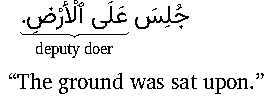
\includegraphics{A-Learners-Grammar-of-Classical-Standard-Arabic_files/figure-latex/unnamed-chunk-32-1.pdf}

\foreignlanguage{arabic}{کُتِبَ بِٱلْقَلَمِ.}\\
\enquote{The pen was written with.}

\subsection{With adverbs of time or place}\label{with-adverbs-of-time-or-place}

Other verbs don't take a direct doee but may be used with an adverb of time or place in the a-state.
(We will study adverbs of time and place in chapter~\ref{adverbs-of-time-and-place}, if Allāh wills.)
Here is an example:

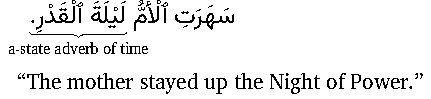
\includegraphics{A-Learners-Grammar-of-Classical-Standard-Arabic_files/figure-latex/unnamed-chunk-33-1.pdf}

When this sentence is converted to an unknown-doer construction then the adverb of time or place can be taken as the deputy doer in the u-state:

\foreignlanguage{arabic}{سُهِرَتْ لَيلَةُ ٱلْقَدْرِ.}\\
\enquote{The Night of Power was stayed up {[}in{]}.}

Note the u-state of \foreignlanguage{arabic}{لَيْلَةُ} \emph{laylatu} as the deputy doer.

\subsection{With the verbal noun of doing}\label{with-the-verbal-noun-of-doing}

The verbal noun of doing, because it is the action being done may be considered a kind of direct doee.
(We will study the use of the verbal noun of doing as a doee in chapter~\ref{absolute-doee}, if Allāh wills.)
For example:

\foreignlanguage{arabic}{فَهِمَ ٱلشَّيْخُ فَهْمًا عَمِيقًا.}\\
\enquote{The old man understood, a deep understanding.}

When such sentences are converted to the unknown-doer verb construction, then the verbal noun of doing may be taken as the deputy doer in the u-state.

\foreignlanguage{arabic}{فُهِمَ فَهْمٌ عَمِيقٌ.}\\
\enquote{A deep understanding was understood.}

\subsection{Requirement of specialization}\label{requirement-of-specialization}

When a prepositional phrase, or an adverb of time or place, or a verbal noun of doing is to be used as a deputy doer in an unknown-doer verb construction, then it is required that they be specialized in meaning, and not used in a general sense. So for example, if we have the sentence:

\foreignlanguage{arabic}{سَهَرَتِ ٱلْأُمُّ لَيلَةً.}\\
\enquote{The mother stayed up a night.}

then because of the non-specialized meaning of \foreignlanguage{arabic}{لَيْلَةً}, such a sentence is typically not suitable for being converted to a unknown-doer verb construction.

\subsection{Choosing the deputy doer}\label{choosing-the-deputy-doer}

If a sentence is to be converted to an unknown-doer verb construction and it has more than one of the following:

\begin{itemize}
\tightlist
\item
  a direct doee
\item
  a specialized prepositional phrase
\item
  a specialized adverb of time or place
\item
  a specialized verbal noun of doing
\end{itemize}

Then only one shall be chosen as the deputy doer. If a direct doee exists, then it is typically chosen. If a direct doee does not exist, then the one desired to be emphasized may be chosen as the deputy doer. For example:

\foreignlanguage{arabic}{سُهِرَ فِي ٱلْمَسْجِدِ لَيلَةَ ٱلْقَدْرِ.}\\
\enquote{The mosque was stayed up in {[}on{]} the Night of Power.}

In the above sentence the prepositional phrase \foreignlanguage{arabic}{فِي ٱلْمَسْجِدِ} was chosen as the deputy doer, and the adverb of time \foreignlanguage{arabic}{لَيْلَةَ} remains, as is, in the a-state.

\section{States of the incomplete-action unknown-doer verb}\label{states-of-the-incomplete-action-unknown-doer-verb}

The
incomplete-action verb unknown-doer verb
has three states, just like the
incomplete-action verb known-doer verb:
The u-state, the a-state, and the ø-state.
The three states are used in the same circumstances, and with the same rules that we have already learned.

So the u-state verb is used for making plain statements:

\foreignlanguage{arabic}{تُذْکَرُ قِصَّةُ ٱلْمَلِکِ فِي کُتُبِ ٱلتَّأْرِيخِ.}\\
\enquote{The story of the king is mentioned in the books of history.}

\foreignlanguage{arabic}{لَا تُرْفَعُ ٱلْأَصْوَاتُ فِي ٱلْمَکْتَبَةِ.}\\
\enquote{Voices are not raised in the library.}

The a-state verb is used for expressing wish or purpose:

\foreignlanguage{arabic}{يَأْمُلُ ٱلْمُسْلِمُونَ أَنْ يُغْفَرُ لَهُمْ.}\\
\enquote{The Muslims hope that they be forgiven.}\\
(Note that \foreignlanguage{arabic}{يُغْفَرَ} has a singular masculine deputy doer because there is no direct doee.)

\foreignlanguage{arabic}{لَنْ تُسْمَعَا.}\\
\enquote{You\textsubscript{2} shall not be heard.}

\foreignlanguage{arabic}{دُفِعَ ٱلْبَابُ حَتَّىٰ يُفْتَحَ.}\\
\enquote{The door was pushed for the result that it open.}

Similarly, the ø-state verb is used in the following cases:

\begin{itemize}
\item
  With \foreignlanguage{arabic}{لَمْ} \enquote{was not}:

  \foreignlanguage{arabic}{لَمْ يُؤْذَنْ لِي أَنْ أَدْخُلَ.}\\
  \enquote{It was not permitted for me that I enter.}
\item
  With \foreignlanguage{arabic}{لَمَّا} \enquote{not yet}

  \foreignlanguage{arabic}{لَمَّا يُکْتَبْ کِتَابٌ فِي هَـٰذَا ٱلْمَوْضُوعِ.}\\
  \enquote{A book has not yet been written in this subject.}
\item
  With \foreignlanguage{arabic}{لِ} for indirect commands:

  \foreignlanguage{arabic}{لِيُسْمَعْ صَوْتُهُ!}\\
  \enquote{Let his voice be heard!}

  There is no verb of command for unknown-doer verbs. So while indirect commands are typically not used for the addressee participant for known-doer verbs (see section~\ref{indirect-commands}), they are the only way to issue commands for the addressee participant in the unknown-doer verb construction:

  \foreignlanguage{arabic}{لِتُنْصَرُوا!}\\
  \enquote{Let you\textsubscript{3m} be aided!}
\end{itemize}

\section{Usage of the unknown-doer verb}\label{usage-of-the-unknown-doer-verb}

There are cases where it is permissible to
use of the unknown-doer verb construction,
and cases where it is \emph{not} permissible to
use of the unknown-doer verb construction. We will explain them below:

\subsection{Permissible use of the unknown-doer verb}\label{permissible-use-of-the-unknown-doer-verb}

There can be a number of reasons why a speaker is forced to, or chooses to, use the unknown-doer verb construction. Among these reasons are:

\begin{enumerate}
\def\labelenumi{\alph{enumi}.}
\item
  When the doer is actually unknown to the speaker. This is the classic use-case, as indicated by the name \emph{unknown-doer verb}. (But, as we shall see below, it is not the only use case.) So, if we say:

  \foreignlanguage{arabic}{کُسِرَتِ ٱلزُّجَاجَةُ.}\\
  \enquote{The glass was broken.}

  then, it may be that we don't know who broke the glass, and that is why we are expressing it in the unknown-doer verb construction.
\item
  When the doer is known to the speaker, but he does not wish to make him known to others. So the same sentence above \foreignlanguage{arabic}{کُسِرَتِ ٱلزُّجَاجَةُ.} could be used when the speaker knows that it was actually \foreignlanguage{arabic}{زَيْد} \enquote{Zayd}, for example, who broke the glass, but the speaker does not wish that others find out that it was Zayd. This itself could be for any reason, for example: the speaker fears Zayd, for fears for Zayd, etc.
\item
  When the speaker wishes to draw attention to the act itself rather than the doer of the act. So we might say:

  \foreignlanguage{arabic}{مُنِعْنَا ٱلدُّخُولَ.}\\
  \enquote{We have been prevented from entering.}

  when we wish to focus on the act of our having been prevented, rather than who prevented us.
\item
  For stylistic reasons, when it is obvious and known who the doer is. For example:

  \foreignlanguage{arabic}{خُلِقَ ٱلْإِنْسَانُ مِنْ ْعَجَلٍ}\\
  \enquote{Man was created of haste {[}i.e., impatience{]}.} (Qurʾān 21:37. Trans. Saheeh International)

  In the above ʾāyah it is known and obvious that Allāh created man.
\item
  In order to glorify the doer. So we might the unknown-doer verb construction to say:

  \foreignlanguage{arabic}{خُلِقَ ٱلْخِنْزِيرُ.}\\
  \enquote{The pig was created.}

  This could be to distance Allāh from being mentioned next to the name of a particularly dirty animal.
\item
  When the doer is not mentioned due to contempt for him. For example:

  \foreignlanguage{arabic}{قُتِلَ أَمِيرُ ٱلْمُؤْمِنِينَ عُمَرُ.}\\
  \enquote{The Commander of the believers, Ɛumar, was killed.}

  In this sentence we chose not to name the killer due to contempt for him.
\end{enumerate}

These reasons are not mutually exclusive, and sometimes the unknown-doer verb construction is used for a combination of them.

\subsection{Impermissible use of the unknown-doer verb}\label{impermissible-use-of-the-unknown-doer-verb}

The unknown-doer verb may not be used when the doer is mentioned with the verb. This is different from English which can use the word \enquote{by} to indicate the doer in a passive voice construction, as in: \enquote{The book was written by Zayd.}. Such a sentence, in Arabic can only be expressed with the known-doer verb construction:

\foreignlanguage{arabic}{کَتَبَ زَيْدٌ ٱلْکِتَابَ.}\\
\emph{kataba zayduni -lkitāb.}\\
\enquote{Zayd wrote the book.}

It may seem like this rule is broken in sentences like:

\foreignlanguage{arabic}{قُتِلَ بِٱلسَّيْفِ.}\\
\emph{qutila bi-ssayf.}\\
\enquote{He was killed by the sword.}

But such is not the case. The known-doer verb constuction would be something like:

\foreignlanguage{arabic}{قَتَلَهُ فُلَانٌ بِٱلسَّيْفِ.}\\
\emph{qatalahu fulānun bi-ssayf.}\\
\enquote{So-and-so killed him with the sword.}

As you can see, \foreignlanguage{arabic}{فُلَان} \enquote{so-and-so} is actually the doer, and \foreignlanguage{arabic}{ٱلسَّيْف} \enquote{the sword} is merely a prepositional phrase indicating the instrument used in the act.

\chapter{The verbal-nouns of the doer and the doee}\label{the-verbal-nouns-of-the-doer-and-the-doee}

FIXME:

\begin{itemize}
\tightlist
\item
  move to later chapter, after \foreignlanguage{arabic}{استفهام} because \foreignlanguage{arabic}{شروط إعمال اسم الفاعل} relies on it.
\item
  add \foreignlanguage{arabic}{الصفة المشبهبة} \emph{verb-like descriptive noun} and its \foreignlanguage{arabic}{عمل}
\item
  add difference in \foreignlanguage{arabic}{إعمال اسم الفاعل} when it has \foreignlanguage{arabic}{ال} and when without.
\item
  add \foreignlanguage{arabic}{اسم المفعول} acting as verb with \foreignlanguage{arabic}{نائب الفاعل}
\end{itemize}

See
+ Wright vol.~ii. p.~65+, and p.~195.
+ \foreignlanguage{arabic}{النحو الوافي} vol 3, p.~246+
+ Howell vol.~4, p 1606+

\section{Introduction}\label{introduction-20}

In the previous chapter we studied the verbal-noun of doing. In this chapter we shall study two more kinds of verbal-nouns. These are the doer verbal-noun and the doee-verbal noun. These, too, are nouns that can give the meaning of the verb they are derived from. In places, they may even replace the verb, thereby adding some nuances in meaning.

The doer verbal-noun gives the meaning of the doer, that is the person doing the action of the verb. For example, for the verb \foreignlanguage{arabic}{قَرَأَ يَقْرَأُ قِرَاءَةً} \enquote{to read}, the doer verbal-noun is \foreignlanguage{arabic}{قَارِئ} \emph{qāriʾ} \enquote{a reader}.

\section{Pattern of the doer verbal-noun}\label{pattern-of-the-doer-verbal-noun}

We saw in the previous chapter that the pattern for the doing verbal-noun for form~1 verbs was very variable. In contrast, the pattern for the doer verbal-noun for form~1 verbs is fixed. It is always on the pasttern \foreignlanguage{arabic}{فَاعِل} \emph{fāɛil}. Also, the doer verbal-noun is modified for gender and number. Its forms its feminine by appending \foreignlanguage{arabic}{ة} thus: \foreignlanguage{arabic}{فَاعِلَة}. It takes sound plurals: the \emph{-ūn} for the masculine, and the \emph{-āt} plural for the feminine. In many case, it may also have broken plurals. Here is a table showing these modifications for the u-state. You should be able to extend them for the a-state and i-state.

\begin{longtable}[]{@{}
  >{\raggedright\arraybackslash}p{(\columnwidth - 4\tabcolsep) * \real{0.3333}}
  >{\raggedright\arraybackslash}p{(\columnwidth - 4\tabcolsep) * \real{0.3333}}
  >{\raggedright\arraybackslash}p{(\columnwidth - 4\tabcolsep) * \real{0.3333}}@{}}
\toprule\noalign{}
\begin{minipage}[b]{\linewidth}\raggedright
Number
\end{minipage} & \begin{minipage}[b]{\linewidth}\raggedright
Masculine
\end{minipage} & \begin{minipage}[b]{\linewidth}\raggedright
Feminine
\end{minipage} \\
\midrule\noalign{}
\endhead
\bottomrule\noalign{}
\endlastfoot
singular & \foreignlanguage{arabic}{فَاعِلٌ} \emph{fāɛilun} & \foreignlanguage{arabic}{فَاعِلَةٌ} \emph{fāɛilatun} \\
dual & \foreignlanguage{arabic}{فَاعِلَانِ} \emph{fāɛilāni} & \foreignlanguage{arabic}{فَاعِلَتَانِ} \emph{fāɛilatāni} \\
plural & \foreignlanguage{arabic}{فَاعِلُونَ} \emph{fāɛilūna} & \foreignlanguage{arabic}{فَاعِلَاتٌ} \emph{fāɛilātun} \\
\end{longtable}

\section{The doer verbal-noun as a noun}\label{the-doer-verbal-noun-as-a-noun}

Like the doing verbal-noun, the doer verbal noun occupies a place that is between a noun and a verb. The basic, most essential, meaning of the doer verbal noun is that of a noun which denotes the doer of the verb.

So, for example, consider the verb \foreignlanguage{arabic}{سَأَلَ يَسْأَلُ سُؤَالًا} \enquote{to question}. Its doer verbal-noun is \foreignlanguage{arabic}{سَائِل}. Since it refers to the doer of this verb, we can translate it as \enquote{a questioner\textsubscript{m.}}.

By itself, the word \foreignlanguage{arabic}{سَائِل} \enquote{a questioner} just denotes a noun. It does not indicate when the doer does the action of the verb: has the questioner already asked the question, is he asking it at present, or will he ask it in the future? So, for example, we can say:

\foreignlanguage{arabic}{سَيَقْدَمُ سَائِلٌ وَسَيَسْأَلُ سُؤَالًا.}\\
\emph{sayaqdamu sāʾilun wasayaqdamu suʾālan.}\\
\enquote{A questioner\textsubscript{m.} will arrive and he will ask a question.}

In the above sentence, the doer verbal-noun is being described as performing the action of the verb in the future.

Here is another example:

\foreignlanguage{arabic}{سَأَلَتِ ٱلْفَقِيهَ سَائِلَةٌ عَنْ أَمْرٍ.}\\
\emph{saʾalati -lfaqīha sāʾilatun ɛan ʾamrin.}\\
\enquote{A questioner\textsubscript{f.} asked the jurist about a matter.}

In the above sentence, the doer verbal-noun is being described as having performed the action of the verb in the past.

Doer verbal-nouns of form~1 verbs, when used with this nounal meaning, often have broken plurals, in addition to their sound plurals. Generally, either could be used in most cases, but the usage of the broken plurals is preferred.

For example, consider the verb \foreignlanguage{arabic}{قَتَلَ يَقْتُلُ قَتْلًا} \enquote{to kill (\foreignlanguage{arabic}{ه} s.o.)}. Its doer verbal-noun is \foreignlanguage{arabic}{قَاتِل} \enquote{a killer\textsubscript{m.}}. Its sound plural is \foreignlanguage{arabic}{قَاتِلُونَ} \emph{qātilūna} and its broken plurals are \foreignlanguage{arabic}{قُتَّال} \emph{quttāl} and \foreignlanguage{arabic}{قَتَلَة} \emph{qatalah}. Any of these could be used but the broken plural is often preferred.

\foreignlanguage{arabic}{هَرَبَ قَتَلَةُ ٱلرَّجُلِ إِلَىٰ مَخْبَئِهِمْ.}\\
\emph{haraba qatalatu -rrajuli ʾilā mak͡hbaʾihim.}\\
\enquote{The killers of the man fled to their hideout.}

\section{The doer verbal-noun as a verb}\label{the-doer-verbal-noun-as-a-verb}

We have learned that the essential meaning of the doer verbal-noun is the doer of the action of the verb from which it is derived. In addition to this essential meaning, the doer verbal-noun can also be used in place of the verb from which it is derived. This is only done when the verb to be replaced is the incomplete-action verb. The doer verbal-noun does not replace the completed-action verb. We will now explain this usage.

\subsection{Usage of the doer verbal-noun as a present tense verb}\label{usage-of-the-doer-verbal-noun-as-a-present-tense-verb}

Consider the following sentence:

\foreignlanguage{arabic}{يَذْهَبُ زَيْدٌ إِلَى ٱلْمَدْرَسَةِ.}\\
\emph{yad͡h·habu zaydun ʾila -lmadrasati.}\\
\enquote{Zayd goes to school.}

The above sentence does not explicitly specify whether Zayd is actually going to school at present, or that he goes to school habitually and not necessarily right now.

If we wish to indicate that Zayd is actually going to school at present we can replace the incomplete-action verb with the indefinite doer verbal-noun. So we get:

\foreignlanguage{arabic}{زَيْدٌ ذَاهِبٌ إِلَى ٱلْمَدْرَسَةِ.}\\
\emph{yad͡h·habu zaydun ʾila -lmadrasati.}\\
\enquote{Zayd is going to school.}

Note that the same preposition \foreignlanguage{arabic}{إِلَىٰ} \emph{ʾilā} \enquote{to} is used with the doer verbal-noun as is used with the verb.
Also note that this is now a subject-information sentence instead of a verbal sentence. \foreignlanguage{arabic}{زَيْدٌ} \emph{zaydun} \enquote{Zayd} is the subject, and \foreignlanguage{arabic}{ذَاهِبٌ} \emph{d͡hāhibun} is part of the information.

This usage of the doer verbal-noun to indicate that the action of the verb is ocurring at present is mostly done for what we call \emph{verbs of posture} and \emph{verbs of motion}.

Verbs of posture denote a static position or activity of the doer's body and include verbs like sitting, standing, lying down, sleeping, etc.

Verbs of motion denote a moving action of the doer's body and include verbs like
going, coming, running, etc.

So, if, for example, we say,

\foreignlanguage{arabic}{زَيْنَبُ جَالِسَةٌ عَلَى هَـٰذَا ٱلْکُرْسِيِّ.}\\
\emph{zaynabu jālisatun ɛala hād͡ha -lkursiyyi.}\\
\enquote{Zaynab is sitting on this chair.}

this indicates that Zaynab is sitting on this chair at present. And if we say,

\foreignlanguage{arabic}{تَجْلِسُ زَيْنَبُ عَلَى هَـٰذَا ٱلْکُرْسِيِّ.}\\
\emph{tajlisu zaynabu ɛala hād͡ha -lkursiyyi.}\\
\enquote{Zaynab sits on this chair.}

this indicates that Zaynab usually sits on this chair.

If this usage of the doer verbal-noun to indicate a present action is mostly only for verbs of posture and motion, how then do we indicate this distinction for other verbs? We have answered this in section {[}TODO: add section to incomplete-action verb{]} where we said that in order to give the meaning that the action of the verb is happening right now, a verbal sentence can be converted to a subject-information sentence.

\subsection{Usage of the doer verbal-noun as a future tense verb}\label{doer-verbal-noun-for-intended-future-action}

The doer verbal-noun may be used in place of the verb it is derived from to indicate an intent on the part of the doer, or to indicate that the action will occur in the future.

This usage of the doer verbal-noun is not just for verbs of posture and motion like the present tense usage. Rather, it is for all verbs in general.

And since intention is something that is mostly expressed by the speaker for himself, rather than for someone else, we will often find this usage with the subject \foreignlanguage{arabic}{أَنَا} \emph{ʾana} \enquote{I}.

\subsubsection{With an indirect doee}\label{with-an-indirect-doee-1}

Here is an example of the usage of the doer verbal-noun as a future tense verb with an indirect doee:

\foreignlanguage{arabic}{أَنَا ذَاهِبٌ إِلَىٰ بَيْتِ صَدِيقِي فِي ٱلصَّبَاحِ.}\\
\emph{ʾana d͡hāhibun ʾilā bayti ṣadīqī fi -ṣṣabāḥi.}\\
\enquote{I'm going to go to my friend's house in the morning.}

In the above sentence it is possible for the phrase
\foreignlanguage{arabic}{فِي ٱلصَّبَاحِ}
\emph{fi -ṣṣabāḥi}
\enquote{in the morning}
to be ommitted for the same meaning. In that case, surrounding context could tell us that the person is intending to go in the future, and is not actually in the process of going there at present.

Here is another example (by a female speaker):

\foreignlanguage{arabic}{عِنْدِي کُرَةٌ فِي ٱلْبَيْتِ فَأَنَا رَاجِعَةٌ إِلَى ٱلْبَيْتِ وَلَاعِبَةٌ بِهَا.}\\
\emph{ɛindī kuratun fi -lbayti faʾana rājiɛatun ʾila -lbayti walāɛibatun bihā.}\\
\enquote{I have a ball at home, so I'm going to go home and play with it.}

\subsubsection{\texorpdfstring{Difference with the particles \foreignlanguage{arabic}{سَـ} \emph{sa-} and \foreignlanguage{arabic}{سَوْفَ} \emph{sawfa}}{Difference with the particles سَـ sa- and سَوْفَ sawfa}}\label{difference-with-the-particles-ux633ux640-sa--and-ux633ux648ux641-sawfa}

We have already learned a method to express a future action using the particles \foreignlanguage{arabic}{سَـ} \emph{sa-} and \foreignlanguage{arabic}{سَوْفَ} \emph{sawfa} with the incomplete-action verb. So we could also have said:

\foreignlanguage{arabic}{سَأَذْهَبُ إِلَىٰ بَيْتِ صَدِيقِي.}\\
\emph{saʾad͡h·habu ʾilā bayti ṣadīqī.}\\
\enquote{I will to go to my friend's house.}

The difference between using the particles \foreignlanguage{arabic}{سَـ} \emph{sa-} and \foreignlanguage{arabic}{سَوْفَ} \emph{sawfa} and using the doer verbal-noun is that using the doer verbal-noun signifies more emphasis, or, as a possible consequence of the emphasis, that the action is more imminent. That is:

\foreignlanguage{arabic}{أَنَا ذَاهِبٌ \ldots{}}\\
\emph{ʾana d͡hāhibun \ldots{}}\\
\enquote{I will {[}definitely{]} go \ldots{}}\\
or\\
\enquote{I'm going to go \ldots{}}

\foreignlanguage{arabic}{سَأَذْهَبُ \ldots{}}\\
\emph{saʾad͡h·habu \ldots{}}\\
\enquote{{[}Soon{]} I will go \ldots{}}

\subsubsection{With a direct doee}\label{with-a-direct-doee-1}

If a verb takes a direct doee, and we wish to use the direct doee with the verb's doer verbal-noun when the doer verbal-noun is acting as a verb, then we may deal with it in one of three ways:

\begin{enumerate}
\def\labelenumi{\arabic{enumi}.}
\item
  The direct doee in a-state following the doer verbal-noun

  The most basic method of dealing with a direct doee of a doer verbal noun is by placing it in the a-state right after the doer verbal-noun. Here is an example,

  \foreignlanguage{arabic}{قَدْ دَخَلَ ٱلْمَدِينَةَ رَجُلٌ شَرِيرٌ. هُوَ \textbf{قَاتِلٌ سُكَّانَهَا}.}\\
  \emph{qad dak͡hala -lmadīnata rajulun s͡harīrun. hua qātilun sukkānahā.}\\
  \enquote{An evil man has entered the city. He is going to kill its residents.}
\item
  The direct doee in i-state annexed to the doer verbal-noun

  The combination of the doer verbal-noun and following direct doee in the a-state is often replaced with an annexation of the doer verbal-noun to the i-state direct doee. So, for example, instead of the above example, we can say:

  \foreignlanguage{arabic}{قَدْ دَخَلَ ٱلْمَدِينَةَ رَجُلٌ شَرِيرٌ. هُوَ \textbf{قَاتِلُ سُكَّانِهَا}.}\\
  \emph{qad dak͡hala -lmadīnata rajulun s͡harīrun. hua qātilu sukkānihā.}\\
  \enquote{An evil man has entered the city. He is going to kill its residents.}

  Note that \foreignlanguage{arabic}{قَاتِلُ سُکَّانِهَا} \emph{qātilu sukkānihā.} can also support the non-verbal meaning of the doer verbal-noun: \enquote{killer of its residents}, i.e., he has already killed its residents in the past. So, when an annexation is used with a doer verbal-noun, we will often need surrounding context to tell us whether the verbal (incomplete-action) meaning is intended, or the noun meaning.

  This usage of annexing the doer verbal-noun to the i-state direct doee instead of employing the more basic usage of the doer verbal-noun and a following a-state direct doee is optional, but fairly common. In fact, when the doer-verbal noun is indefinite and nūnated, and the direct doee begins with \foreignlanguage{arabic}{ٱَلْ} \emph{ʾal}, then the annexation usage becomes predominant over the basic a-state usage. So we will be more likely to see:

  \foreignlanguage{arabic}{أَنَا فَاعِلُهُ.}\\
  \emph{ʾana fāɛiluhu.}

  instead of:

  \foreignlanguage{arabic}{أَنَا فَاعِلٌ إِيَّاهُ.}\\
  \emph{ʾana fāɛilun ʾiyyāhu.}

  for the meaning: \enquote{I will do it.} Note again, that the latter sentence could also support the nounal meaning of the doer-verbal noun: \enquote{I am its doer.}, i.e., \enquote{the one who did it.}

  Similarly, it will be more common to find:

  \foreignlanguage{arabic}{هُوَ قَاتِلُ ٱلنَّاسِ.}\\
  \emph{huwa qātilu -nnāsi.}

  instead of:

  \foreignlanguage{arabic}{هُوَ قَاتِلٌ ٱلنَّاسَ.}\\
  \emph{huwa qātiluni -nnāsa.}

  for the meaning: \enquote{He is going to kill the people.} Note, once again, that the former sentence also supports the meaning: \enquote{He is the people's killer.}, i.e., \enquote{the one who killed them}, and that context would be needed to tell us which of the two meanings is intended.

  The annexation of a doer verbal-noun to its direct doee in the i-state is not the kind of \enquote{proper} annexation that we have learned so far. In fact, it is called an \emph{improper annexation} and we shall study it in more detail in chapter \hyperref[todo]{TODO}, if Allāh wills.
\item
  Quite similar to what we learned in section~@ref(the-direct-doee-in-i-state-preceded-by-the-preposition-\%D9\%84-li) for doing verbal-nouns, the direct doee can follow the doer verbal-noun in the i-state preceded by the preposition \foreignlanguage{arabic}{لِ} \emph{li}.

  This is often optional, as an alternative to the above two methods. For example,

  \foreignlanguage{arabic}{هُوَ قَاتِلٌ لَهُمْ.}\\
  \emph{huwa qātilun lahum.}\\
  \enquote{He will kill them.}

  Using \foreignlanguage{arabic}{لِ} \emph{li} in this manner is also a technique to move the direct doee before the doer verbal-noun for effect, if desired. For example,

  \foreignlanguage{arabic}{هُوَ لَهُمْ قَاتِلٌ.}\\
  \emph{huwa lahum qātilun.}\\
  \enquote{He will kill them.}
\end{enumerate}

\subsection{The definite doer verbal-noun as a verb}\label{the-definite-doer-verbal-noun-as-a-verb}

So far we have seen only an indefinite doer verbal-noun being used with the meaning of an incomplete-action verb. However, the definite doer verbal-noun, too, can give this meaning. The meaning is often in the present tense. Here are some examples:

With an indirect doee:

\foreignlanguage{arabic}{قَدِمَ زَيْدٌ ٱلذَّاهِبُ إِلَى ٱلْجَامِعَةِ.}\\
\emph{qadima zayduni -d͡hd͡hāhibu ʾila -ljāmiɛati.}\\
\enquote{Zayd, the one who goes to the university, has arrived.}

With a direct doee in the a-state:

\foreignlanguage{arabic}{هَرَبْتُ مِنَ ٱلْأَسَدِ ٱلْآکِلُ ٱلْإِنْسَانَ.}\\
\emph{harabtu mina -lʾasadi -lʾākilu -lʾinsāna.}\\
\enquote{I fled from the lion, the one that eats man.}

With a direct doee in the i-state preceded by the preposition \foreignlanguage{arabic}{لِ} \emph{li}:

\foreignlanguage{arabic}{سَيَنْجَحُ ٱلطَّالِبُ ٱلتَّارِکُ لِلَّهْوِ.}\\
\emph{sayanjaḥu -ṭṭālibu -ttāriku lillahwi.}\\
\enquote{The student, the one who leaves idle amusement, will succeed.}

\subsection{Plurals of the doer verbal-noun when used as a verb}\label{plurals-of-the-doer-verbal-noun-when-used-as-a-verb}

We mentioned in section~\ref{the-doer-verbal-noun-as-a-noun} that doer-verbal nouns when used with their nounal meaning often have broken plurals along with their sound plural.
We gave the example of the doer verbal-noun
\foreignlanguage{arabic}{قَاتِل} \emph{qātil} \enquote{a killer\textsubscript{m.}} with the sound plural is \foreignlanguage{arabic}{قَاتِلُونَ} \emph{qātilūna} and the broken plurals \foreignlanguage{arabic}{قُتَّال} \emph{quttāl} and \foreignlanguage{arabic}{قَتَلَة} \emph{qatalah}.

When the doer verbal-noun is used as a verb, only the sound plural is permitted to be used, and the broken plurals, if any are not used. So we can only say:

\foreignlanguage{arabic}{هُمْ قَاتِلُونَ ٱلنَّاسَ.}\\
\emph{hum qātilūna -nnāsa.}\\
and\\
\foreignlanguage{arabic}{هُمْ قَاتِلُو ٱلنَّاسِ.}\\
\emph{hum qātilu -nnāsi.}\\
for\\
\enquote{They will kill the people.}\\
not, for example\\
\(\times\)~\foreignlanguage{arabic}{هُمْ قُتَّالٌ ٱلنَّاسَ.}

(In the second sentence, the \foreignlanguage{arabic}{ن} of \foreignlanguage{arabic}{قَاتِلُونَ} is ommitted because it is an annexe noun).

\section{The doee verbal-noun}\label{the-doee-verbal-noun}

The doee verbal-noun for form~1 verbs is on the pattern \foreignlanguage{arabic}{مَفْعُول} \emph{mafɛūl}. It carries the meaning of the person or thing to whom the action of the verb has been done. For example, the doee verbal-noun for the verb
\foreignlanguage{arabic}{قَتَلَ يَقْتُلُ قَتْلًا} \enquote{to kill (\foreignlanguage{arabic}{ه} s.o.)}
is \foreignlanguage{arabic}{مَقْتُول} \emph{maqtūl} and means \enquote{a killed person}.

\subsection{The plural of the doee verbal noun}\label{the-plural-of-the-doee-verbal-noun}

The doee verbal-noun almost always takes the sound plurals \emph{-ūn} for masculine intelligent beings, and \emph{-āt} otherwise. Therefore the plural of the doee verbal-noun
\foreignlanguage{arabic}{مَقْتُول} \emph{maqtūl} \enquote{a killed person\textsubscript{m.}} is \foreignlanguage{arabic}{مَقْتُولُونَ} \emph{maqtūlūna} \enquote{killed persons\textsubscript{m.}}.
and the plural of the doee verbal-noun
\foreignlanguage{arabic}{مَقْتُولَة} \emph{maqtūlah} \enquote{a killed person\textsubscript{f.}} is \foreignlanguage{arabic}{مَقْتُولَات} \emph{maqtūlāt} \enquote{killed persons\textsubscript{f.}}.

There are a only a few doee verbal-nouns that, as an exception, have broken plurals. The broken plural for these exceptions is than always on the pattern \textsuperscript{2}\foreignlanguage{arabic}{مَفَاعِيل} \emph{mafāɛīl}\textsuperscript{2}. For example, the doee verbal-noun for the verb
\foreignlanguage{arabic}{لَعَنَ يَلْعَنُ لَعْنًا} \enquote{to curse (\foreignlanguage{arabic}{ه} s.o.)} is \foreignlanguage{arabic}{مَلْعُون} \emph{malɛūn} \enquote{accursed} and its plural is \textsuperscript{2}\foreignlanguage{arabic}{مَلَاعِين} \emph{malāɛīn}\textsuperscript{2}.

\subsection{Usage of the doee verbal-noun}\label{usage-of-the-doee-verbal-noun}

Much of what has been said regarding the doer verbal-noun applies to the doee verbal-noun as well: The doee verbal-noun may be used with a verbal meaning for the incomplete-action verb only. So if we say:

\foreignlanguage{arabic}{هُوَ مَقْتُولٌ.}\\
\emph{huwa maqtūl}

with a verbal meaning, then it means \enquote{He will be killed.} And if we say it using its nounal meaning, then it means \enquote{He is the person killed.}

Unlike the doer verbal-noun which can take doees, since the doee verbal-noun is itself the doee, there is no question of it taking other doees. So this does simplify matters.

\subsection{The doee verbal-nouns of indirect doee verbs}\label{the-doee-verbal-nouns-of-indirect-doee-verbs}

Consider the verb
\foreignlanguage{arabic}{سَأَلَ يَسْأَلُ سُؤَالًا} \enquote{to question (\foreignlanguage{arabic}{ه عن} s.o. about s.th.)}.

Here it is used in a sentence:

\foreignlanguage{arabic}{سَأَلَ زَيْدٌ زَيْنَبَ عَنْ حَادِثَةٍ.}\\
\emph{saʾala zaydun zaynaba ɛan ḥādit͡hah.}\\
\enquote{Zayd questioned Zaynab about an accident.}

In this sentence, \foreignlanguage{arabic}{زَيْدٌ} \emph{zaydun} \enquote{Zayd} is the doer. The corresponding doer verbal-noun that refers to him is \foreignlanguage{arabic}{سَائِل} \emph{sāʾil} \enquote{a questioner\textsubscript{m.}}.
Next, \foreignlanguage{arabic}{زَيْنَبَ} \emph{zaynaba} \enquote{Zaynab} is the direct doee. The corresponding doee verbal-noun that refers to her is \foreignlanguage{arabic}{مَسْؤُولَة} \emph{masʾūlah} \enquote{a questioned person\textsubscript{f.}}.
But how, now, do we refer to the indirect doee: \foreignlanguage{arabic}{حَادِثَةٍ} \emph{ḥadit͡hatin} \enquote{an accident}? The answer is that the doee verbal-noun referring to this indirect doee is \foreignlanguage{arabic}{مَسْؤُول عَنْهَا} \emph{masʾūl ɛanhā} \enquote{a thing\textsubscript{f.} questioned about}.

Let's analyze this term \foreignlanguage{arabic}{مَسْؤُول عَنْهَا} \emph{masʾūl ɛanhā} \enquote{a thing questioned about} carefully. The first word is \foreignlanguage{arabic}{مَسْؤُول} \emph{masʾūl} which shall always be singular masculine, regardless of the gender and number of the indirect doee. The second word is \foreignlanguage{arabic}{عَنْهَا} \emph{ɛanhā} \enquote{about it}. Here \foreignlanguage{arabic}{عَنْ} \emph{ɛan} is the same preposition that has been used with the verb. And \foreignlanguage{arabic}{هَا} \emph{hā} is the pronoun that refers to the indirect doee \foreignlanguage{arabic}{حَادِثَةٍ} \emph{ḥadit͡hatin} \enquote{an accident}. If the number or gender of the indirect doee were to change then this would be reflected in this pronoun.

So, for example, if we say,

\foreignlanguage{arabic}{نَظَرَ زَيْدٌ إِلَى ٱلرِّجَالِ.}\\
\emph{naḍ͡hara zaydun ʾila -rrijāli.}\\
\enquote{Zayd looked at the men.}

then, the doee verbal-noun that refers to \foreignlanguage{arabic}{ٱلرِّجَالِ} \emph{ʾarrijāli} \enquote{the men} is \foreignlanguage{arabic}{مَنْظُور إِلَيْهِمْ} \emph{manḍ͡hūr ʾilayhim} \enquote{persons\textsubscript{m.} looked at}.

If doee verbal-nouns of indirect doees are used in sentences then it is the first word (in this case \foreignlanguage{arabic}{مَنْظُور} \emph{manḍ͡hūrun}) that changes for definiteness and state (but not for gender or number, as already discussed). Here are some examples:

From the verb \foreignlanguage{arabic}{لَعِبَ يَلْعَبُ لَعِبًا} \enquote{to play (\foreignlanguage{arabic}{هـ} s.th.)}:

\foreignlanguage{arabic}{هَـٰذِهِ ٱلْکُرىٰ هِيَ ٱلْمَلْعُوبُ بِهَا.}\\
\emph{hād͡hi -lkurā hiya -lmalɛūbu bihā.}\\
\enquote{These balls are the ones played with.}

From the verb \foreignlanguage{arabic}{أَمَرَ يَأْمُرُ أَمْرًا} \enquote{to order (\foreignlanguage{arabic}{ه} s.o. \foreignlanguage{arabic}{ب} to do s.th.)}:

\foreignlanguage{arabic}{فَعَلَ ٱلْغُلَامُ ٱلْمأمُورَ بِهِنَّ.}\\
\emph{faɛala -lg͡hulāmu -lmaʾmūra bihinna.}\\
\enquote{The boy did the {[}things{]} ordered to do.}

(Remember that the feminine plural pronouns may be used to refer to plural non-intelligent beings, regardless of their grammatical gender, in order to indicate plurality.)

Having said all this, in practice, you may find that indirect doees are sometimes treated as direct doees when forming their doee verbal-noun. This is especially common when forming plurals for terms that are very common. So instead of referring to \enquote{{[}things{]} ordered to do} in the above example as
\foreignlanguage{arabic}{ٱَلْمأمُورَ بِهِنَّ}
\emph{ʾalmaʾmūra bihinna}, you may find the word \foreignlanguage{arabic}{ٱَلْمَأْمُورَاتِ} \emph{ʾalmaʾmūrāti} used instead.

TODO: The doee verbal noun for indirect doees may have some ambiguity with the doee verbal for direct doees. \foreignlanguage{arabic}{مسؤول عنه} can also be \enquote{the person who is asked about it} where the pronoun has been substituted for a noun, for example \foreignlanguage{arabic}{مسؤول عن الأمر} . In this case it is the word \foreignlanguage{arabic}{مسؤول} which will be feminized and pluralized. \foreignlanguage{arabic}{المسؤولون عنه} \enquote{the persons asked about it.}

For that matter \foreignlanguage{arabic}{ساءل عنه} is also valid as \enquote{the questioner about it}.

\section{Doer and doee verbal-nouns re-used as adjectival-nouns}\label{doer-and-doee-verbal-nouns-re-used-as-adjectival-nouns}

Doer and doee verbal-nouns are often re-used as adjectival-nouns with meanings that are directly formed from their doer and doee meaning respectively. Here are some examples:

\begin{longtable}[]{@{}
  >{\raggedright\arraybackslash}p{(\columnwidth - 4\tabcolsep) * \real{0.5833}}
  >{\raggedright\arraybackslash}p{(\columnwidth - 4\tabcolsep) * \real{0.1667}}
  >{\raggedright\arraybackslash}p{(\columnwidth - 4\tabcolsep) * \real{0.2500}}@{}}
\toprule\noalign{}
\begin{minipage}[b]{\linewidth}\raggedright
Verb
\end{minipage} & \begin{minipage}[b]{\linewidth}\raggedright
Doer/doee verbal-noun
\end{minipage} & \begin{minipage}[b]{\linewidth}\raggedright
Adjectival-noun meaning
\end{minipage} \\
\midrule\noalign{}
\endhead
\bottomrule\noalign{}
\endlastfoot
\foreignlanguage{arabic}{نَعُمَ يَنْعُمَ نُعُومَةً} \enquote{to be soft} & \foreignlanguage{arabic}{نَاعِم} & \enquote{soft} \\
\foreignlanguage{arabic}{يَبِسَ يَيْبَسُ يُبُوسَةً} \enquote{to be dried up} & \foreignlanguage{arabic}{يَابِس} & \enquote{dried up} \\
\foreignlanguage{arabic}{حَضَرَ يَحْضُرُ حُضُورًا} \enquote{to be present} & \foreignlanguage{arabic}{حَاضِر} & \enquote{present (attending)} \\
\foreignlanguage{arabic}{جَمَعَ يَجْمَعُ جَمْعًا} \enquote{to gather (\foreignlanguage{arabic}{هـ} s.th.)} & \foreignlanguage{arabic}{جَامِع} & \enquote{comprehensive} \\
\foreignlanguage{arabic}{لَمَعَ يَلْمَعُ لَمْعًا وَلَمَعَانًا} \enquote{to be shiny} & \foreignlanguage{arabic}{لَامِع} & \enquote{shiny} \\
\foreignlanguage{arabic}{فَتَحَ يَفْتَحُ فَتْحًا} \enquote{to open (\foreignlanguage{arabic}{هـ} s.th.)} & \foreignlanguage{arabic}{مَفْتُوح} & \enquote{open} \\
\foreignlanguage{arabic}{شَهَرَ يَشْهَرُ شَهْرًا} \enquote{to make famous (\foreignlanguage{arabic}{ه، هـ} s.o., s.th.)} & \foreignlanguage{arabic}{مَشْهُور} & \enquote{famous} \\
\end{longtable}

\subsection{Genderizability of doer and doee verbal-nouns when re-used as adjectival-nouns}\label{genderizability-of-doer-and-doee-verbal-nouns-when-re-used-as-adjectival-nouns}

When a doer or doee verbal-noun is re-used as an adjectival-noun, then it generally retains its genderizability. For example,

\foreignlanguage{arabic}{بَابٌ مَفَتُوحٌ}\\
\emph{bābun maftūḥun}\\
\enquote{an open door}

and

\foreignlanguage{arabic}{نَافِذَةٌ مَفَتُوحَةٌ}\\
\emph{nāfid͡hatun maftūḥatun}\\
\enquote{an open window}

If, however, the adjectival-noun is only applicable to females, then, only a female adjectival-noun is formed but, peculiarly, without the feminine marker \foreignlanguage{arabic}{ة}. The most common example is from the verb:
\foreignlanguage{arabic}{حَمَلَ يَحْمِلٌ حَمْلًا} \enquote{to carry (\foreignlanguage{arabic}{هـ} s.th.)}. The doer verbal-noun is \foreignlanguage{arabic}{حَامِل} \emph{ḥāmil} \enquote{a carrier}. The adjectival-noun formed from the doer verbal-noun is \enquote{pregnant}, but because it is only applicable to females, it does not get the feminine marker \foreignlanguage{arabic}{ة}. For example,

\foreignlanguage{arabic}{ٱَلْمَرْأَةُ حَامِلٌ.}\\
\emph{ʾalmarʾatu ḥāmil.}\\
\enquote{The woman is pregnant.}

This does not affect the doer verbal-noun when it is not used with this adjectival-noun meaning. For example,

\foreignlanguage{arabic}{ٱَلْمَرْأَةُ حَامِلَةُ ٱلْمَاءِ.}\\
\emph{ʾalmarʾatu ḥāmilatu -lmāʾ.}\\
\enquote{The woman will carry the water.}\\
or\\
\enquote{The woman is the water-carrier.}

\subsection{Corresponding with English adjectives}\label{corresponding-with-english-adjectives}

Sometimes both the doer verbal-noun and the doee verbal-noun are used in Arabic with distinct meanings where we would use the same word in English. For example, the verb
\foreignlanguage{arabic}{عَقَلَ يَعْقِلُ عَقْلًا} \emph{ɛaqala yaɛqilu ɛaqlan} means \enquote{to make sense (\foreignlanguage{arabic}{هـ} of s.th.)}.
Its doer verbal-noun \foreignlanguage{arabic}{عَاقِل} \emph{ɛāqil} means \enquote{one who makes sense (of something)} and may be re-used as an adjectival noun meaning \enquote{sensible} when it refers to a person who makes sense of something. For example,

\foreignlanguage{arabic}{زَيْدٌ غُلَامٌ عَاقِلٌ.}\\
\emph{zaydun g͡hulāmun ɛāqil.}\\
\enquote{Zayd is a sensible boy.}

Its doee verbal-noun \foreignlanguage{arabic}{مَعْقُول} \emph{maɛqūl} means \enquote{something which makes sense} and may be re-used as an adjectival noun meaning \enquote{sensible} when it refers to a something which makes sense. For example,

\foreignlanguage{arabic}{هَـٰذَا مَنْهَجٌ مَعْقُولٌ.}\\
\emph{hād͡hā manhajun maɛqūl.}\\
\enquote{This is a sensible approach.}

\section{Doer and doee verbal-nouns re-used as common nouns}\label{doer-and-doee-verbal-nouns-re-used-as-common-nouns}

The doer verbal-noun is often re-used as a common noun with a meaning that is either directly, or indirectly related to the meaning of the verb. For example, the doer verbal-noun of the verb \foreignlanguage{arabic}{سَأَلَ يَسْأَلُ سُؤَالًا} \emph{saʾala yasʾalu suʾālan} is \foreignlanguage{arabic}{سَائِل} \enquote{a questioner} with the sound plural \foreignlanguage{arabic}{سَائِلُونَ} \emph{sāʾilūna} and the broken plurals \foreignlanguage{arabic}{سُؤَّال} \emph{suʾʾāl} and \foreignlanguage{arabic}{سَأَلَة} \emph{saʾalah}.

The word \foreignlanguage{arabic}{سَائِل} \emph{sāʾil} \enquote{a questioner} is re-used with the meaning \enquote{a beggar}. The association in meaning is that a beggar continually asks people for money.

The re-use of a doer verbal-noun or doee verbal-noun as a common noun does not prevent it from being used with its doer/doee or verbal meaning any more.
\foreignlanguage{arabic}{سَائِل} \emph{sāʾil} may be used to mean both \enquote{a questioner} and \enquote{a beggar}, and context will help us determine which of the meanings is intended.

When a doer verbal-noun is re-used as a common noun then only the broken plural, if it exists, may be used. The sound plural is only permitted to be used if no broken plurals exist. Here are some more examples of doer verbal-nouns re-used as common nouns:

\begin{longtable}[]{@{}
  >{\raggedright\arraybackslash}p{(\columnwidth - 6\tabcolsep) * \real{0.5000}}
  >{\raggedright\arraybackslash}p{(\columnwidth - 6\tabcolsep) * \real{0.1429}}
  >{\raggedright\arraybackslash}p{(\columnwidth - 6\tabcolsep) * \real{0.1429}}
  >{\raggedright\arraybackslash}p{(\columnwidth - 6\tabcolsep) * \real{0.2143}}@{}}
\toprule\noalign{}
\begin{minipage}[b]{\linewidth}\raggedright
Verb
\end{minipage} & \begin{minipage}[b]{\linewidth}\raggedright
Doer/doee verbal-noun
\end{minipage} & \begin{minipage}[b]{\linewidth}\raggedright
Plural
\end{minipage} & \begin{minipage}[b]{\linewidth}\raggedright
Common noun meaning
\end{minipage} \\
\midrule\noalign{}
\endhead
\bottomrule\noalign{}
\endlastfoot
\foreignlanguage{arabic}{عَلِمَ يَعْلَمُ عِلْمًا} \enquote{to know (\foreignlanguage{arabic}{هـ} s.th.)} & \foreignlanguage{arabic}{عَالِم} & \textsuperscript{2}\foreignlanguage{arabic}{عُلَمَاء} & \enquote{a scholar} \\
\foreignlanguage{arabic}{طَلَبَ يَطْلُبُ طَلَبًا} \enquote{to seek (\foreignlanguage{arabic}{هـ} s.th.)} & \foreignlanguage{arabic}{طَالِب} & \foreignlanguage{arabic}{طُلَّاب، طَلَبَة} & \enquote{a student} \\
\foreignlanguage{arabic}{لَعِبَ يَلْعَبُ لَعِبًا} \enquote{to play (\foreignlanguage{arabic}{هـ} s.th.)} & \foreignlanguage{arabic}{لَاعِب} & \foreignlanguage{arabic}{لَاعِبُونَ} & \enquote{a player} \\
\foreignlanguage{arabic}{جَمَعَ يَجْمَعُ جَمْعًا} \enquote{to gather (\foreignlanguage{arabic}{هـ} s.th.)} & \foreignlanguage{arabic}{جَامِعَة} & \foreignlanguage{arabic}{جَامِعَات} & \enquote{a university} \\
\foreignlanguage{arabic}{جَمَعَ يَجْمَعُ جَمْعًا} \enquote{to gather (\foreignlanguage{arabic}{هـ} s.th.)} & \foreignlanguage{arabic}{جَامِع} & \textsuperscript{2}\foreignlanguage{arabic}{جَوَامِع} & \enquote{a mosque (in which the Friday prayers are performed)} \\
\foreignlanguage{arabic}{حَدَثَ يَحْدُثُ حُدُوثًا} \enquote{to happen} & \foreignlanguage{arabic}{حَادِثَةٌ} & \textsuperscript{2}\foreignlanguage{arabic}{حَوَادِث} & \enquote{an accident} \\
\foreignlanguage{arabic}{شَرِبَ يَشْرَبُ شُرْبًا} \enquote{to drink (\foreignlanguage{arabic}{هـ} s.th.)} & \foreignlanguage{arabic}{شَارِب} & \textsuperscript{2}\foreignlanguage{arabic}{شَوَارِب} & \enquote{a moustache} \\
\foreignlanguage{arabic}{سَحَلَ يَسْحَلُ سَحْلًا} \enquote{to abrade (\foreignlanguage{arabic}{هـ} s.th.)} & \foreignlanguage{arabic}{سَاحِلٌ} & \textsuperscript{2}\foreignlanguage{arabic}{سَوَاحِل} & \enquote{a seashore} \\
\foreignlanguage{arabic}{ضَمِنَ يَضْمَنُ ضَمَانًا} \enquote{to guarantee (\foreignlanguage{arabic}{هـ} s.th.)} & \foreignlanguage{arabic}{مَضْمُوxk} & \textsuperscript{2}\foreignlanguage{arabic}{مَضَامِين} & \enquote{a content (of a letter, etc.)} \\
\foreignlanguage{arabic}{دَخَلَ يَدْخُلُ دُخُولًا} \enquote{to enter} & \foreignlanguage{arabic}{دَاخِل} & none & \enquote{inside} \\
\foreignlanguage{arabic}{خَرَجَ يَخْرُجُ خُرُوجًا} \enquote{to exit} & \foreignlanguage{arabic}{خَارِج} & none & \enquote{outside} \\
\end{longtable}

The last two \foreignlanguage{arabic}{دَاخِلٌ} \enquote{inside} and \foreignlanguage{arabic}{خَارِجٌ} \enquote{outside} are notable. Here, for example, is how they can be used:

\foreignlanguage{arabic}{غَسَلَ ٱلْکُوبَ مِنْ دَاخِلٍ.}\\
\emph{g͡hasala -lkūba min dāk͡hilin.}\\
\enquote{He washed the tumbler from inside.}

\subsection{Genderizability of doer and doee verbal-nouns when re-used as common nouns}\label{genderizability-of-doer-and-doee-verbal-nouns-when-re-used-as-common-nouns}

When a doer or doee verbal-noun is re-used as a common noun, then it loses its genderizability. For example, if we wish to say \enquote{The building is a university.} we will say:

\foreignlanguage{arabic}{ٱَلْبِنَاءُ جَامِعَةٌ.}\\
\emph{ʾalbināʾu jāmiɛah.}\\
\enquote{The building is a university.}

We cannot masculinize \foreignlanguage{arabic}{جَامِعَة} \emph{jāmiɛah} \enquote{a university} to \foreignlanguage{arabic}{جَامِع} \emph{jāmiɛ} in order to make it match the gender of \foreignlanguage{arabic}{بِنَاء} \emph{bināʾ} (masc.) \enquote{a building}. Were we to do so, then
\foreignlanguage{arabic}{جَامِع} \emph{jāmiɛ} would get interpreted with either:

\begin{enumerate}
\def\labelenumi{\arabic{enumi}.}
\item
  Its doer verbal-noun meaning \enquote{a gatherer}:

  \enquote{The building is a gatherer.}

  which doesn't make sense as a sentence.
\item
  Or, with the common noun meaning of \foreignlanguage{arabic}{جَامِع} \emph{jāmiɛ}, if one happens to exist. There is such a meaning in this case: \enquote{a mosque (in which the Friday prayers are performed)}. So then we would get:

  \foreignlanguage{arabic}{ٱَلْبِنَاءُ جَامِعٌ.}\\
  \emph{ʾalbināʾu jāmiɛun.}\\
  \enquote{The building is a mosque (in which the Friday prayers are performed).}
\item
  Or, with the adjectival noun meaning of \foreignlanguage{arabic}{جَامِع} \emph{jāmiɛ}, if one happens to exist. There is such a meaning in this case: \enquote{comprehensive}. So then we would get:

  \foreignlanguage{arabic}{ٱَلْبِنَاءُ جَامِعٌ.}\\
  \emph{ʾalbināʾu jāmiɛun.}\\
  \enquote{The building is comprehensive.}
\end{enumerate}

None of these give the original meaning we intended: \enquote{The building is a university.} So, in summary,
once a doer or doee verbal-noun is re-used as a common noun, it loses its genderizability.

Having said this, when a doer verbal-noun is re-used as a common noun that applies to humans, both the masculine and feminine common-noun typically exist together. So for example,

\foreignlanguage{arabic}{عَالِم} \emph{ɛālim} is re-used as the common-noun for \enquote{a (male) scholar} with the plural \textsuperscript{2}\foreignlanguage{arabic}{عُلَمَاء} \emph{ɛulamāʾ}.
And\\
\foreignlanguage{arabic}{عَالِمَة} \emph{ɛālimah} is re-used as the common-noun for \enquote{a (female) scholar} with the plural \foreignlanguage{arabic}{عَالِمَات} \emph{ɛālimāt}.

In such cases, i.e., when applicable to humans, the dictionary will generally only list, and supply the definition for the masculine common-noun. The reader is expected to know that its feminine exists and how to form it.

There are exceptions, however. The verb \foreignlanguage{arabic}{جَرَىٰ يَجْرِي جَرْيًا} \emph{jarā yajrī jaryan} \enquote{to run} is formed from the root \foreignlanguage{arabic}{«جري»}. This is a weak root because of the letter \foreignlanguage{arabic}{ي} in it, and we will study it in more detail later in chapter~\ref{roots-with-weak-final-letter}. In any case, its feminine doer verbal-noun is \foreignlanguage{arabic}{جَارِيَة} \emph{jāriyah} and is re-used for the common noun meaning \enquote{a girl}. The masculine doer verbal noun is not re-used as a common noun for the meaning \enquote{a boy}.

\chapter{The connected noun}\label{the-connected-noun}

\section{Introduction}\label{introduction-21}

Consider the sentence:

\foreignlanguage{arabic}{رَأَيْتُ ٱلرَّجُلَ.}\\
\enquote{I saw the man.}

If the listener (or reader) can identify
the individual referred to by the noun \enquote{the man}
(maybe from a pre-existing mutual understanding with the speaker),
then there is no problem with this sentence.
But often, further clarification is needed for the listener to correctly identify the individual to whom the speaker is referring.
This further clarification can be provided in a number of ways.

One way is to use an adjectival noun to describe the noun. For example:

\foreignlanguage{arabic}{رَأَيْتُ ٱلرَّجُلَ ٱلطَّوِيلَ.}\\
\enquote{I saw the \emph{tall} man.}

Another way is to use a pointing noun, thus:

\foreignlanguage{arabic}{رَأَيْتُ ذَ~ٰلِکَ ٱلرَّجُلَ.}\\
\enquote{I saw \emph{that} man.}

But sometimes, a whole sentence is needed to provide the needed identification.
In this case, Arabic uses what is called a \emph{connected noun} and a \emph{connector}.
This example should help you understand what we mean:

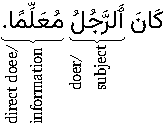
\includegraphics{A-Learners-Grammar-of-Classical-Standard-Arabic_files/figure-latex/unnamed-chunk-34-1.pdf}

In the above sentence, the connected noun is \foreignlanguage{arabic}{ٱَلَّذِي} \emph{ʾallad͡hī}.
It is applied to singular masculine nouns, like \foreignlanguage{arabic}{ٱلرَّجُل}.
By itself it may be translated as \enquote{the one\textsubscript{1m} that/which/who/whom}.
It is called a connected noun because it must be directly followed by a qualifying sentence that connects to it.

The qualifying sentence is called the connector and it contains the necessary information for the listener to correctly identify the individual intended by the speaker.''
The connector in the above example is the sentence \foreignlanguage{arabic}{لَقِيتُهُ بِٱلْأَمْسِ} \enquote{I met him yesterday.}

Note by the way, that we did not translate the pronoun \enquote{him} in our original translation (above).
This is because it would sound unnatural in English to say: \enquote{I saw the {[}specific{]} man (whom) I met \emph{him} yesterday.}
But this pronoun is an essential part of the Arabic connector and is called the \emph{link-back pronoun}.
We will deal with it in section~\ref{link-back-pronoun} later in this chapter.

There are two types of connected nouns:

\begin{enumerate}
\def\labelenumi{\arabic{enumi}.}
\tightlist
\item
  The specific connected nouns
\item
  The general connected nouns
\end{enumerate}

We will study both these types separately within this chapter.

\section{The specific connected nouns}\label{the-specific-connected-nouns}

The specific connected nouns have a significance which is restricted to a specific individual or category of individuals,
and its connector should contain sufficient information to identify that specific individual.

The specific connected nouns is a group of nouns where each noun is applied to a gender and number of individuals. They are:

\begin{longtable}[]{@{}
  >{\raggedright\arraybackslash}p{(\columnwidth - 2\tabcolsep) * \real{0.1500}}
  >{\raggedright\arraybackslash}p{(\columnwidth - 2\tabcolsep) * \real{0.8500}}@{}}
\toprule\noalign{}
\begin{minipage}[b]{\linewidth}\raggedright
Connected noun
\end{minipage} & \begin{minipage}[b]{\linewidth}\raggedright
Description
\end{minipage} \\
\midrule\noalign{}
\endhead
\bottomrule\noalign{}
\endlastfoot
\foreignlanguage{arabic}{ٱَلَّذِي} \emph{ʾallad͡hī} & Singular masculine. For both intelligent and non-intelligent beings. Rigid. Only one \foreignlanguage{arabic}{ل} in its spelling. \\
\foreignlanguage{arabic}{ٱَلَّتِي} \emph{ʾallatī} & Singular feminine. For both intelligent and non-intelligent beings. Also used for plural non-intelligent beings of both genders. Rigid. Only one \foreignlanguage{arabic}{ل} in its spelling. \\
\foreignlanguage{arabic}{ٱَللَّذَانِ} \emph{ʾallad͡hānī} & Dual masculine. For both intelligent and non-intelligent beings. Flexible: \foreignlanguage{arabic}{ٱَللَّذَيْنِ} \emph{ʾallad͡hayni} in the a- and i-states. Two \foreignlanguage{arabic}{ل}'s in its spelling. \\
\foreignlanguage{arabic}{ٱَللَّتَانِ} \emph{ʾallatānī} & Dual feminine. For both intelligent and non-intelligent beings. Flexible: \foreignlanguage{arabic}{ٱَللَّتَيْنِ} \emph{ʾallatayni} in the a- and i-states. Two \foreignlanguage{arabic}{ل}'s in its spelling. \\
\foreignlanguage{arabic}{ٱَلَّذِينَ} \emph{ʾallad͡hīna} & Plural masculine. For both intelligent beings. Rigid. Only one \foreignlanguage{arabic}{ل} in its spelling. \\
\foreignlanguage{arabic}{ٱَللَّاتِي} \emph{ʾallātī} & For plural feminine intelligent beings. Also used for non-intelligent beings of both genders but \foreignlanguage{arabic}{ٱَلَّتِي} is more common there. Rigid. Two \foreignlanguage{arabic}{ل}'s in its spelling. Has the following variants: \foreignlanguage{arabic}{ٱَللَّاتِ} \emph{ʾallāti}, \foreignlanguage{arabic}{ٱَللَّائِي} \emph{ʾallāʾī}, \foreignlanguage{arabic}{ٱَللَّوَاتِي} \emph{ʾallawātī} \\
\end{longtable}

\subsection{Grammatical position of the specific connected noun}\label{grammatical-position-of-the-specific-connected-noun}

Consider again the same example:

\foreignlanguage{arabic}{رَأَيْتُ ٱلرَّجُلَ ٱلَّذِي لَقِيتُهُ بِٱلْأَمْسِ.}\\
\enquote{I saw the {[}specific{]} man whom I met yesterday.}

In this example, the connected noun
\foreignlanguage{arabic}{ٱَلَّذِي} \emph{ʾallad͡hī}
is a describer (in the a-state) to the described noun
\foreignlanguage{arabic}{ٱلرَّجُلَ}.
Because
\foreignlanguage{arabic}{ٱَلَّذِي}
is a rigid noun, it will appear the same in all states without any change to its ending.

As a describer, the connected noun may also come as the last in a series of describers, and can also be combined with a pointing noun.
For example:

\foreignlanguage{arabic}{رَأَيْتُ ذَ~ٰلِکَ ٱلرَّجُلَ ٱلطَّوِيلَ ٱلَّذِي لَقِيتُهُ بِٱلْأَمْسِ.}\\
\enquote{I saw that {[}specific{]} tall man whom I met yesterday.}

But connected nouns need not only occur as describers.
They may occur in various grammatical positions.
Here are some examples:

As a subject:

\foreignlanguage{arabic}{وَالَّذِينَ يَکْنِزُونَ ٱلذَّهَبَ وَٱلْفِضَّةَ وَلَا يُنْفِقُونَهَا فِي سَبِيلِ ٱللَّـٰهِ فَبَشِّرْهُمْ بِعَذَابٍ أَلِيمٍ}\\
\enquote{And those who hoard gold and silver and spend it not in the way of Allāh - give them tidings of a painful punishment.}\\
9:34

As an information:

\foreignlanguage{arabic}{خِيَارُ أَئِمَّتِکُمُ الَّذِينَ تُحِبُّونَهُمْ وَيُحِبُّونَکُمْ}\\
\enquote{The best of your rulers are the ones whom you love and who love you}
{[}Ṣaḥīḥ Muslim:1855{]}

\foreignlanguage{arabic}{هُنَّ اللَّوَاتِي عَلَى الْمِنْبَرِ}\\
\enquote{They are the ones which (are) on the pulpit.}\\
{[}Sunan al-Dārimī:36{]}

As a doer:

\foreignlanguage{arabic}{قَدْ بَلَغَنَا ٱلَّذِي قُلْتُمُوهُ.}\\
\enquote{The {[}specific{]} one (thing) that you said has reached us.}

As a doee:

\foreignlanguage{arabic}{رَبَّنَا أَرِنَا ٱللَّذَيْنِ أَضَلَّانَا مِنَ ٱلْجِنِّ وَٱلْإِنْسِ}\\
\enquote{Our Lord, show us those who misled us of the jinn and men}\\
41:29

Following a preposition:

\foreignlanguage{arabic}{أَوْ کَٱلَّذِي مَرَّ عَلَىٰ قَرْيَةٍ}\\
\enquote{Or {[}consider such an example{]} as the one who passed by a township}\\
2:259

As a base noun in an annexation:

\foreignlanguage{arabic}{قَدْ سَمِعَ ٱللَّـٰهُ قَوْلَ ٱلَّتِي تُجَادِلُکَ فِي زَوْجِهَا}\\
\enquote{Certainly has Allāh heard the speech of the one who argues {[}i.e., pleads{]} with you, {[}O Muḥammad{]}}\\
58:1

\section{The connector and the link-back pronoun}\label{link-back-pronoun}

The connector is (typically) a sentence that directly follows the connected noun.
As we mentioned in the introduction,
the connector provides clarifying information for the listener (or reader) to identify the individual referred to by the connected noun.

In the connector is a pronoun that refers back to the connected noun.
This pronoun is called the \emph{link-back pronoun}.
and it is an essential (though not always apparent) part of the connector.

Let us identify some of the link-back pronouns in the examples we have given.

\foreignlanguage{arabic}{وَالَّذِينَ يَکْنِزُونَ ٱلذَّهَبَ وَٱلْفِضَّةَ}\\
\enquote{And those who hoard gold and silver}\\
Link-back pronoun: the plural masculine doer pronoun \foreignlanguage{arabic}{و} in \foreignlanguage{arabic}{يَکْنِزُونَ}

\foreignlanguage{arabic}{خِيَارُ أَئِمَّتِکُمُ الَّذِينَ تُحِبُّونَهُمْ}\\
\enquote{The best of your rulers are the ones whom you love and who love you}\\
Link-back pronoun: the plural masculine doee attached pronoun \foreignlanguage{arabic}{هُمْ} in \foreignlanguage{arabic}{تُحِبُّونَهُمْ}

\foreignlanguage{arabic}{قَدْ بَلَغَنَا ٱلَّذِي قُلْتُمُوهُ.}\\
\enquote{The {[}specific{]} one (thing) that you said has reached us.}\\
Link-back pronoun: the singular masculine doee attached pronoun \foreignlanguage{arabic}{هُ} in \foreignlanguage{arabic}{قُلْتُمُوهُ}

\foreignlanguage{arabic}{رَبَّنَا أَرِنَا ٱللَّذَيْنِ أَضَلَّانَا مِنَ ٱلْجِنِّ وَٱلْإِنْسِ}\\
\enquote{Our Lord, show us those who misled us of the jinn and men}\\
Link-back pronoun: the dual masculine doer pronoun \foreignlanguage{arabic}{ا} in \foreignlanguage{arabic}{أَضَلَّانَا}

\foreignlanguage{arabic}{أَوْ کَٱلَّذِي مَرَّ عَلَىٰ قَرْيَةٍ}\\
\enquote{Or {[}consider such an example{]} as the one who passed by a township}\\
Link-back pronoun: the implied singular masculine doer pronoun \enquote{he} in \foreignlanguage{arabic}{مَرَّ}

\foreignlanguage{arabic}{قَدْ سَمِعَ ٱللَّـٰهُ قَوْلَ ٱلَّتِي تُجَادِلُکَ فِي زَوْجِهَا}\\
\enquote{Certainly has Allāh heard the speech of the one who argues {[}i.e., pleads{]} with you, {[}O Muḥammad{]}}\\
Link-back pronoun: the implied singular feminine doer pronoun \enquote{she} in \foreignlanguage{arabic}{تُجَادِلُکَ}

\subsection{Matching the link-back pronoun with the connected noun}\label{matching-the-link-back-pronoun-with-the-connected-noun}

The link-back pronoun generally matches the connected noun in gender and number.
For example, in the sentence
\foreignlanguage{arabic}{وَالَّذِينَ يَکْنِزُونَ ٱلذَّهَبَ وَٱلْفِضَّةَ}
\enquote{And those who hoard gold and silver}\\
the plural masculine link-back pronoun \foreignlanguage{arabic}{و} in \foreignlanguage{arabic}{يَکْنِزُونَ}
matches the plural masculine connected noun \foreignlanguage{arabic}{ٱلَّذِينَ}.

However, there is an exception to this rule.
And that is when the connected noun refers to the speaker or the addressed person, like
\foreignlanguage{arabic}{أَنَا ٱلَّذِي}, or \foreignlanguage{arabic}{أَنْتُمُ ٱلَّذِينَ}, etc.
In these cases, the link-back pronoun may optionally:

\begin{enumerate}
\def\labelenumi{\roman{enumi}.}
\tightlist
\item
  either match the pronoun for the speaker or addressed person (as the case may be),
\item
  or match the connected noun and thus be a pronoun for absent person.
\end{enumerate}

The former is generally more common but both options are permissible.
For example:

\foreignlanguage{arabic}{أَنَا ٱلَّذِي حَضَرْتُ.}\\
Link-back pronoun: the singular masculine doer pronoun for the speaker \foreignlanguage{arabic}{تُ} in \foreignlanguage{arabic}{حَضَرْتُ}\\
or\\
\foreignlanguage{arabic}{أَنَا ٱلَّذِي حَضَرَ.}\\
Link-back pronoun: the implied singular masculine doer pronoun for the absent person \enquote{he} in \foreignlanguage{arabic}{حَضَرَ}\\
\enquote{I am the one (who) was present.}

Here are some examples from Classical Arabic:

\foreignlanguage{arabic}{أَنَا ٱلَّذِي سَمَّتْنِ أُمِّي حَيْدَرَهْ}\\
\enquote{I am the one whom my mother named Ḥaydarah}\\
(The link-back pronoun is the speaker person's doee pronoun in \foreignlanguage{arabic}{سَمَّتْنِ}, which is an abbreviation of \foreignlanguage{arabic}{سَمَّتْنِي} \enquote{she named me}.)

\foreignlanguage{arabic}{فَقَالَ مُوسَى يَا آدَمُ أَنْتَ الَّذِي خَلَقَکَ اللَّهُ بِيَدِهِ}\\
\enquote{Mūsā said: O Ādam, you are the one whom Allāh created with His Hand}\\
tirmidhi:2134\\
(The link-back pronoun is the addressed person's doee pronoun \foreignlanguage{arabic}{کَ} in \foreignlanguage{arabic}{خَلَقَکَ}.)

There is one circumstance where matching the link-back pronoun to the (absent person) connected-noun is mandated.
And that is when the connected noun is the called-out person using the particle \foreignlanguage{arabic}{أَيُّهَا} or \foreignlanguage{arabic}{أَيَّتُهَا}.
For example,

\foreignlanguage{arabic}{يَاأَيُّهَا ٱلَّذِينَ آمَنُوا}\\
\enquote{O you who have believed}\\
not\\
\(\times\) \foreignlanguage{arabic}{يَاأَيُّهَا ٱلَّذِينَ آمَنْتُمْ}

Similarly,

\foreignlanguage{arabic}{يَاأَيُّهَا الَّذِي نُزِّلَ عَلَيْهِ الذِّکْرُ}\\
\enquote{O you upon whom the message has been sent down}\\
15:6

\subsection{Omitting the link-back pronoun}\label{omitting-the-link-back-pronoun}

The link-back pronoun is frequently omitted, and its meaning is then implicit, in some cases:

\begin{enumerate}
\def\labelenumi{(\alph{enumi})}
\item
  When the linker pronoun is a detached pronoun which is the u-state subject of a subject-information sentence, whose information is:

  \begin{enumerate}
  \def\labelenumii{(\roman{enumii})}
  \item
    A prepositional phrase. For example:

    \foreignlanguage{arabic}{نَامَ ٱلَّذِي فِي ٱلْغُرْفَةِ.}\\
    \enquote{The one who (is) in the room has slept.}

    The connector is the incomplete sentence \foreignlanguage{arabic}{فِي ٱلْغُرْفَةِ} \enquote{(is) in the room}.
    With the link-back pronoun restored, the sentence is

    \foreignlanguage{arabic}{نَامَ ٱلَّذِي هُوَ فِي ٱلْغُرْفَةِ.}
  \item
    An adverbial phrase. For example:

    \foreignlanguage{arabic}{تَکَلَّمَ ٱلَّذِي عِنْدَکَ.}\\
    \enquote{The one who (is) with you spoke.}

    (Remember that \foreignlanguage{arabic}{عِنْدَ} is technically a noun used adverbially, not a preposition.)
    The connector is the incomplete sentence \foreignlanguage{arabic}{عِنْدَکَ} \enquote{(is) with you}.
    With the link-back pronoun restored, the sentence is

    \foreignlanguage{arabic}{تَکَلَّمَ ٱلَّذِي هُوَ عِنْدَکَ.}
  \end{enumerate}

  In such cases, the incomplete sentence connector implcitly includes the meaning of a verb which is usually the verb \enquote{being}, like \enquote{is}, \enquote{are}, \enquote{am}, etc.
\item
  When the link-back pronoun is an attached pronoun for the direct doee. For example:

  \foreignlanguage{arabic}{قَدْ بَلَغَنَا ٱلَّذِي قُلْتُمْ.}\\
  \enquote{The one (thing) that you said has reached us.}

  With the link-back pronoun restored, the sentence is

  \foreignlanguage{arabic}{قَدْ بَلَغَنَا ٱلَّذِي قُلْتُمُوهُ.}
\item
  \begin{enumerate}
  \def\labelenumii{(\roman{enumii})}
  \item
    When the link-back pronoun is the base noun in an annexation whose annex noun is a verbal noun of the doer or the doee implying a present or future meaning. For example:

    \foreignlanguage{arabic}{أَخَافُ مِنْهُ ٱلظُّلْمَ ٱلَّذِي هُوَ فَاعِلٌ.}\\
    \enquote{I fear from him the wrong that he will do.}

    With the link-back pronoun restored, the sentence is\\
    \foreignlanguage{arabic}{أَخَافُ مِنْهُ ٱلظُّلْمَ ٱلَّذِي هُوَ فَاعِلُهُ.}
  \item
    When the link-back pronoun is attached to a preposition or adverb, and the same preposition or adverb has already been used (with the same meaning) with the connecting noun or its described noun. The preposition/adverb is omitted along with its attached pronoun. For example:

    \foreignlanguage{arabic}{سِرْتُ فِي ٱلْحَدِيقَةِ ٱلَّتِي سِرْتَ.}\\
    \enquote{I walked in the (same) garden {[}in{]} which you walked.}

    With the link-back pronoun restored, the sentence is\\
    \foreignlanguage{arabic}{سِرْتُ فِي ٱلْحَدِيقَةِ ٱلَّتِي سِرْتَ فِيهَا.}

    \foreignlanguage{arabic}{مَرَرْتُ بِٱلَّذِي مَرَّ سُلَيْمَانُ.}\\
    \enquote{I passed by the (same) one that Sulaymān did.}

    With the link-back pronoun restored, the sentence is\\
    \foreignlanguage{arabic}{مَرَرْتُ بِٱلَّذِي مَرَّ بِهِ سُلَيْمَانُ.}
  \end{enumerate}
\end{enumerate}

\subsection{Separating the connector from the connected noun}\label{separating-the-connector-from-the-connected-noun}

Generally, the connector directly follows the connected noun, as in all the examples we have given so far.
However, the connector may be separated from the connected noun by one of the following:

\begin{enumerate}
\def\labelenumi{\roman{enumi}.}
\item
  An oath. For example:

  \foreignlanguage{arabic}{جَاءَ ٱلَّذِي وَٱللَّـٰه قَهَرَ ٱلْأَعْدَاءَ.}\\
  \enquote{The one who - by Allāh - overpowered the enemies has come.}
\item
  A sentence calling out to someone. For example,

  \foreignlanguage{arabic}{أَنْتَ ٱلَّذِي يَا زَيْدُ فَتَحْتَ ٱلْبَابَ.}\\
  \enquote{You are the one - O Zayd - who opened the door.}
\item
  A parenthetical clause, which is a sentence within the main sentence that adds information to it, but which can be omitted without affecting the completeness of the main sentence. For example:

  \foreignlanguage{arabic}{قَدِمَ ٱلَّذِي أَطَالَ ٱللَّـٰهُ عُمْرَهُ أَحْسَنَ إِلَيَّ.}\\
  \enquote{The one who - may Allah lengthen his age - was good to me has arrived.}

  \foreignlanguage{arabic}{قَدِمَ ٱلَّذِي وَهُوَ مُبْتَسِمٌ أَحْسَنَ إِلَيَّ.}\\
  \enquote{The one who - and he is smiling - was good to me has arrived.}
\end{enumerate}

\section{The general connected nouns}\label{the-general-connected-nouns}

The general connected nouns are unrestricted in significance, and may be applied to any individual who fits the criteria given in the connector.
The two main general connected nouns are:

\begin{enumerate}
\def\labelenumi{\arabic{enumi}.}
\tightlist
\item
  \foreignlanguage{arabic}{مَنْ} \emph{man}. Typically used for intelligent beings and translated as \enquote{who}.
\item
  \foreignlanguage{arabic}{مَا} \emph{mā}. Typically used for non-intelligent beings and translated as \enquote{what}.
\end{enumerate}

There are also some other rarely or dialectally used general connected nouns. These are \foreignlanguage{arabic}{أَيّ} \emph{ʾayy}, \foreignlanguage{arabic}{ذُو} \emph{d͡hū}, and \foreignlanguage{arabic}{ذَا} \emph{d͡hā}. We will not be going over these.

Unlike the specific connected nouns (\foreignlanguage{arabic}{ٱَلَّذِي}, etc.),
the general connected nouns do not vary for number and gender.

For example:

\foreignlanguage{arabic}{أُحِبُّّ مَنْ يَعْدِلُ}\\
\enquote{I love {[}him{]} who is just.}

\foreignlanguage{arabic}{أُحِبُّّ مَنْ يَعْدِلُونَ}\\
\enquote{I love {[}them{]} who are just.}

\foreignlanguage{arabic}{ٱِصْنَعْ مَا بَدَا لَکَ.}\\
\enquote{Do what seems (good) to you.}

\foreignlanguage{arabic}{مَرَرْتُ بِمَا يُعْجِبُکَ.}\\
\enquote{I passed by what will please you.}

\subsection{\texorpdfstring{\foreignlanguage{arabic}{مَنْ} and \foreignlanguage{arabic}{مَا} after prepositions}{مَنْ and مَا after prepositions}}\label{ux645ux646-and-ux645ux627-after-prepositions}

When \foreignlanguage{arabic}{مَنْ} and \foreignlanguage{arabic}{مَا} are directly preceded by the prepositions \foreignlanguage{arabic}{مِنْ} and \foreignlanguage{arabic}{عَنْ}, these prepositions lose their \foreignlanguage{arabic}{ن} and are joined to the following noun with the noun's \foreignlanguage{arabic}{م} doubled.
For example:
\foreignlanguage{arabic}{مَمَّنْ} \emph{mimman},
\foreignlanguage{arabic}{مَمَّا} \emph{mimmā},
\foreignlanguage{arabic}{عَمَّنْ} \emph{ɛamman},
\foreignlanguage{arabic}{عَمَّا} \emph{ɛammā}.

The preposition \foreignlanguage{arabic}{فِي} is also often (though not always) optionally attached to these connected nouns, thus: \foreignlanguage{arabic}{فِيمَنْ} \emph{fīman}, \foreignlanguage{arabic}{فِيمَا} \emph{fīmā}.

The remaining prepositions follow the normal rules: \foreignlanguage{arabic}{عَلَى مَا}, \foreignlanguage{arabic}{کَمَنْ}, etc.
But we will see, if Allāh wills, in chapter~\ref{questions}, that \foreignlanguage{arabic}{مَا} and \foreignlanguage{arabic}{مَنْ} are also used as question nouns, in which case the rules of joining prepositions to them will differ.

\subsection{The link-back pronoun for the general connected nouns}\label{the-link-back-pronoun-for-the-general-connected-nouns}

The general connected nouns
\foreignlanguage{arabic}{مَنْ}
and
\foreignlanguage{arabic}{مَا}
are themselves singular masculine in number and gender.
However, they can be used to signify persons or things of any number and gender.

Their link-back pronouns can then, optionally:

\begin{enumerate}
\def\labelenumi{\roman{enumi}.}
\item
  Either match the gender and number of the persons or things meant by the connected noun. For example:

  \foreignlanguage{arabic}{وَمِنْهُمْ مَنْ يَسْتَمِعُونَ إِلَيْکَ}\\
  \enquote{And among them are those who listen to you}\\
  10:42

  \foreignlanguage{arabic}{قَدْ خَابَتْ مَنْ فَعَلَتْ ذَلِکَ مِنْهُنَّ وَخَسِرَتْ}\\
  \enquote{She has thwarted herself, whoever did that from them\textsubscript{3f}, and lost.}\\
  {[}Jāmiɛ al-Tirmid͡hī:3318{]}

  Note also how, in this example how, in addition to the feminine link-back doer pronouns in \foreignlanguage{arabic}{فَعَلَتْ} and \foreignlanguage{arabic}{خَسِرَتْ},
  the feminine gender of the person signified by \foreignlanguage{arabic}{مَنْ} has also caused the \foreignlanguage{arabic}{تْ} of femininity to be added to the verb \foreignlanguage{arabic}{خَابَ} (of which \foreignlanguage{arabic}{مَنْ} is the doer noun).

  \foreignlanguage{arabic}{جَمَعْتُ مِنَ ٱلْوَرَقِ مَا سَقَطْنَ.}
  \enquote{I gathered what fell from the leaves.}

  \foreignlanguage{arabic}{صَلِّ مِنَ ٱلرَّکَعَاتِ مَا يَتَيَسَّرْنَ.}\\
  or\\
  \foreignlanguage{arabic}{صَلِّ مِنَ ٱلرَّکَعَاتِ مَا تَتَيَسَّرُ.}\\
  \enquote{Pray from the units (of prayer) what is easy.}
\item
  Or be singular masculine to match the connected noun itself. This is generally more common for \foreignlanguage{arabic}{مَا}. For example:

  \foreignlanguage{arabic}{وَمِنْهُم مَّن يُؤْمِنُ بِهِۦ وَمِنْهُم مَّن لَّا يُؤْمِنُ بِهِۦ ۚ}\\
  \enquote{And of them are those who believe in it, and of them are those who do not believe in it.}\\
  10:40

  \foreignlanguage{arabic}{جَمَعْتُ مِنَ ٱلْوَرَقِ مَا سَقَطَ.}
  \enquote{I gathered what fell from the leaves.}

  \foreignlanguage{arabic}{صَلِّ مِنَ ٱلرَّکَعَاتِ مَا يَتَيَسَّرُ.}\\
  \enquote{Pray from the units (of prayer) what is easy.}

  \foreignlanguage{arabic}{لَمْ أَجِدْ مَا أَعْتَذِرُ بِهِ}\\
  \enquote{I did not find what I (could) make an excuse for with}.
\end{enumerate}

Both options can be utilized together as well. For example:

\foreignlanguage{arabic}{بَلَىٰ مَنْ أَسْلَمَ وَجْهَهُۥ لِلَّهِ وَهُوَ مُحْسِنٌۭ فَلَهُۥٓ أَجْرُهُۥ عِندَ رَبِّهِۦ وَلَا خَوْفٌ عَلَيْهِمْ وَلَا هُمْ يَحْزَنُونَ}\\
\enquote{Yes, {[}on the contrary{]}, whoever submits his face {[}i.e., self{]} in Islām to Allāh while being a doer of good will have his reward with his Lord. And no fear will there be concerning them, nor will they grieve.}\\
2:112

\foreignlanguage{arabic}{فَمَن تَبِعَ هُدَايَ فَلَا خَوْفٌ عَلَيْهِمْ وَلَا هُمْ يَحْزَنُونَ}\\
\enquote{whoever follows My guidance - there will be no fear concerning them, nor will they grieve.}\\
2:38

\subsubsection{Omitting the link-back pronoun}\label{omitting-the-link-back-pronoun-1}

The same guidelines for omitting the link-back pronouns, which we learned for the specific connected nouns, apply also to the general connected nouns.
For example:

\foreignlanguage{arabic}{وَلَهُ مَن فِي السَّمَاوَاتِ وَالْأَرْضِ}\\
\enquote{To Him belongs whoever is in the heavens and the earth.}\\
21:19\\
(for \foreignlanguage{arabic}{مَنْ هُوَ فِي ٱلسَّمَوَاتِ وَٱلْأَرْضِ})

\foreignlanguage{arabic}{هَـٰذَا مَا کَنَزْتُمْ لِأَنْفُسِکُمْ}\\
\enquote{This is what you hoarded for yourselves}\\
9:35\\
(for \foreignlanguage{arabic}{مَا کَنَزْتُمُوهُ})

\foreignlanguage{arabic}{فَٱقْضِ مَا أَنتَ قَاضٍ}\\
\enquote{So decree whatever you are to decree.}\\
20:72\\
(for \foreignlanguage{arabic}{مَا أَنْتَ قَاضِيهِ})

\foreignlanguage{arabic}{أَنَا عِنْدَ مَنْ أَنْتَ.}\\
\enquote{I am at his {[}house{]} at whose you (are).}\\
(for \foreignlanguage{arabic}{مَنْ أَنْتَ عِنْدَهُ})

\subsection{\texorpdfstring{Applicability of \foreignlanguage{arabic}{مَا} and \foreignlanguage{arabic}{مَنْ} to intelligent and non-intelligent beings}{Applicability of مَا and مَنْ to intelligent and non-intelligent beings}}\label{applicability-of-ux645ux627-and-ux645ux646-to-intelligent-and-non-intelligent-beings}

As we mentioned earlier, \foreignlanguage{arabic}{مَنْ} is typically used to refer to intelligent beings.
And \foreignlanguage{arabic}{مَا} is typically used to refer to non-intelligent beings.
However, there are some circumstances in which these roles can differ.

\foreignlanguage{arabic}{مَنْ}
may be used for non-intelligent beings when a non-intelligent being is compared with an intelligent being.
For example,

\foreignlanguage{arabic}{وَاللَّهُ خَلَقَ کُلَّ دَابَّةٍ مِّن مَّاءٍ ۖ}\\
\foreignlanguage{arabic}{فَمِنْهُم مَّن يَمْشِي عَلَىٰ بَطْنِهِ}\\
\foreignlanguage{arabic}{وَمِنْهُم مَّن يَمْشِي عَلَىٰ رِجْلَيْنِ}\\
\foreignlanguage{arabic}{وَمِنْهُم مَّن يَمْشِي عَلَىٰ أَرْبَعٍ ۚ}\\
\enquote{Allāh has created every {[}living{]} creature from water. And of them are those that move on their bellies, and of them are those that walk on two legs, and of them are those that walk on four.}

\foreignlanguage{arabic}{مَنْ}
may also be used for non-intelligent beings when
attributes usually applicable to intelligent beings are applied to a non-intelligent being.
For example:

\foreignlanguage{arabic}{أَسِرْبَ الْقَطَا، هَلْ مَنْ يُعِيرُ جَنَاحَه * لَعَلِّي إِلَىٰ مَنْ قَدْ هَوِيتُ أَطِيرُ}\\
O flock of birds, is there who will lend his wing\\
that perhaps I may fly to whom I love\\
\foreignlanguage{arabic}{أَ}: \enquote{O},
\foreignlanguage{arabic}{سِرْب}: \enquote{flock},
\foreignlanguage{arabic}{قَطَا}: a species of bird,
\foreignlanguage{arabic}{هَلْ}: \enquote{is there?},
\foreignlanguage{arabic}{يُعِيرُ}: \enquote{lend},
\foreignlanguage{arabic}{جَنَاح}: \enquote{wing},
\foreignlanguage{arabic}{لَعَلِّي}: \enquote{Perhaps I},
\foreignlanguage{arabic}{هَوِيتُ}: \enquote{I love},
\foreignlanguage{arabic}{أَطِيرُ}: \enquote{I fly}.

\foreignlanguage{arabic}{مَنْ}
may also be used for non-intelligent beings when
there is a mixed group including both intelligent and non-intelligent beings,
and the intelligent beings are given preference.
For example:

\foreignlanguage{arabic}{وَلِلَّهِ يَسْجُدُ مَن فِى ٱلسَّمَـٰوَٰتِ وَٱلْأَرْضِ}\\
\enquote{And to Allāh prostrates whoever is within the heavens and the earth}\\
13:15

Similarly, \foreignlanguage{arabic}{مَا} may, in some circumstances, be used for intelligent beings.
This may be when
there is a mixed group including both intelligent and non-intelligent beings,
and the non-intelligent beings are given preference because of their larger number.
For example:

\foreignlanguage{arabic}{يُسَبِّحُ لِلَّهِ مَا فِي السَّمَاوَاتِ وَمَا فِي الْأَرْضِ}\\
\enquote{Whatever is in the heavens and whatever is on the earth is exalting Allāh}\\
62:1

\foreignlanguage{arabic}{مَا} may also be used for intelligent beings when
the person being referred to is vague to the speaker.
For example:

\foreignlanguage{arabic}{رَبِّ إِنِّي نَذَرْتُ لَکَ مَا فِي بَطْنِي مُحَرَّرًا}\\
\enquote{My Lord, indeed I have pledged to You what is in my womb, consecrated {[}for Your service{]}}\\
3:35

\foreignlanguage{arabic}{مَا} may also be used for intelligent beings when
the characteristics of an intelligent being are highlighted when referring to them. For example:

\foreignlanguage{arabic}{فَانکِحُوا مَا طَابَ لَکُم مِّنَ النِّسَاءِ}\\
\enquote{then marry those that please you of {[}other{]} women}\\
4:3

\subsection{Grammatical position of the general connected nouns}\label{grammatical-position-of-the-general-connected-nouns}

The general connected noun may occur in various grammatical positions.
Here are some examples:

As a subject:

\foreignlanguage{arabic}{ما عِنْدَکُمْ يَنْفَدُ}\\
\enquote{Whatever you have will end}\\
16:96

As an information:

\foreignlanguage{arabic}{مَالُکَ مَا قَدَّمْتَ، وَمَالُ وَارِثِکَ مَا أَخَّرْتَ}\\
\enquote{Your wealth is what you have sent forward, and the wealth of your inheritors is what you have left behind.}\\
adab:153

As a doer:

\foreignlanguage{arabic}{فَعَلَهُ مَنْ هُوَ خَيْرٌ مِنِّي}\\
\enquote{it was done by one who was better than I}\\
bukhari:668

As a doee:

\foreignlanguage{arabic}{اعْمَلُوا مَا شِئْتُمْ}\\
\enquote{Do whatever you will}\\
41:40

Following a preposition:

\foreignlanguage{arabic}{وَأَغْنِنِي بِفَضْلِکَ عَمَّنْ سِوَاکَ}\\
\enquote{and make me independent from (all) who are besides You}\\
tirmidhi:3563

As a base noun in an annexation:

\foreignlanguage{arabic}{هُمْ شَرُّ مَنْ خَلَقَ ٱللَّـٰهُ.}\\
\enquote{They are the most evil of whom Allah has created.}

\foreignlanguage{arabic}{مَا تَرَىٰ رَأْيَ مَا نَرَىٰ.}\\
\enquote{You do not think what we think.}\\
(literally: \enquote{You do not opine the opinion of what we opine.})

\foreignlanguage{arabic}{أَمْرَ مَا تَحْذَرُ}\\
\enquote{the matter of which you are wary}

Unlike the specific connected nouns
(\foreignlanguage{arabic}{ٱَلَّذِي}, etc),
the general connected nouns do not occur as describers.

So while we can say:

\foreignlanguage{arabic}{مَرَرْتُ بِٱلرَّجُلِ ٱلَّذِي أَحْسَنَ إِلَيّ.}\\
\enquote{I passed by the man who was good to me.}

we cannot say:

\(\times\) \foreignlanguage{arabic}{مَرَرْتُ بِٱلرَّجُلِ مَنْ أَحْسَنَ إِلَيّ.}

We will have to say instead:

\foreignlanguage{arabic}{مَرَرْتُ بِمَنْ أَحْسَنَ إِلَيّ.}

\subsection{\texorpdfstring{Use with the preposition \foreignlanguage{arabic}{مِنْ}}{Use with the preposition مِنْ}}\label{use-with-the-preposition-ux645ux646}

The preposition \foreignlanguage{arabic}{مِنْ} is frequently used with the general connected nouns to restrict the applicability of the connected noun to a group or type.
For example:

\foreignlanguage{arabic}{سَأُعْطِيهِ مَا عِنْدِي مِنْ خُبْزٍ.}\\
\enquote{I will give him what I have of bread.}

\foreignlanguage{arabic}{مَنْ دَخَلَ ٱلشَّأْمَ مِنَ ٱلْعَرَبِ}\\
\enquote{Those Arabs who entered Syria}\\
(literally: \enquote{Who entered Syria from the Arabs})

\foreignlanguage{arabic}{فَانکِحُوا مَا طَابَ لَکُم مِّنَ النِّسَاءِ}\\
\enquote{then marry those that please you of {[}other{]} women}\\
4:3

\subsection{Use with a repeated word to express vagueness or uncertainty}\label{use-with-a-repeated-word-to-express-vagueness-or-uncertainty}

The general connected nouns
\foreignlanguage{arabic}{مَنْ} and \foreignlanguage{arabic}{مَا}
are used with a word that is repeated to express a vague or uncertain quantity or quality.
For example:

\foreignlanguage{arabic}{هُمْ مَا هُمْ}\\
\enquote{They are what they are.}

\foreignlanguage{arabic}{نَزَلَ مَنْ نَزَلَ مِنْهُمْ}\\
\enquote{Some of them came down.}\\
(literally: Came down who came down from them.'')

\foreignlanguage{arabic}{جَمَعْتُ مَا جَمَعْتُ}\\
\enquote{I gathered what I gathered.}

\section{Omitting the connected noun and/or the connector}\label{omitting-the-connected-noun-andor-the-connector}

TODO. See النحو الوافي

\section{Sentences without connected nouns}\label{sentences-without-connected-nouns}

There are some sentences where we might expect a connected noun but which are always, or often (as the case may be), expressed in Arabic without a connected noun. These sentences are of different types:

\subsection{Sentences with indefinite nouns needing a qualifying sentence}\label{sentences-with-indefinite-nouns-needing-a-qualifying-sentence}

When an indefinite noun needs a qualifying sentence, it is natural in English to insert \enquote{that}, \enquote{which}, \enquote{who}, etc. between the noun and the following sentence. For example, \enquote{I passed by a man \emph{who} was sleeping.}

In Arabic, however, we will not use any connected noun in such sentences.
This is because the connected nouns are considered definite nouns.
And therefore they may not be a describer to an indefinite noun.
So while we can say:

\foreignlanguage{arabic}{مَرَرْتُ بِٱلرَّجُلِ ٱلَّذِي يَنَامُ.}\\
\enquote{I passed by the man who is sleeping.}

we cannot say

\(\times\) \foreignlanguage{arabic}{مَرَرْتُ بِرَجُلٍ ٱلَّذِي يَنَامُ.}

Instead, we put the qualifying sentence directly after the indefinite noun. The qualifying sentence will then not be a connector, but will itself be the describer to the described noun:

\foreignlanguage{arabic}{مَرَرْتُ بِرَجُلٍ يَنَامُ.}\\
\enquote{I passed by a man (who) is sleeping.}

Here is another example:

\foreignlanguage{arabic}{جَلَسْتُ فِي مَجْلِسٍ قَدْ رُشَّ بِمَاءِ ٱلْوَرْدِ.}\\
\enquote{I sat in a sitting (that) had been sprinkled with rose-water.}

A connected noun can, however, follow an indefinite noun, if we intend to start a separate sentence with it, or if it is a \emph{replacement} (see chapter~\ref{the-replacement}). For example.

\foreignlanguage{arabic}{وَابْعَثْهُ مَقَامًا مَحْمُودًا الَّذِي وَعَدْتَهُ}\\
\enquote{Resurrect him to a praiseworthy station, the one that you promised him}\\
bukhari:614

\foreignlanguage{arabic}{وَيْلٌ لِّکُلِّ هُمَزَةٍ لُّمَزَةٍ}\\
\foreignlanguage{arabic}{الَّذِي جَمَعَ مَالًا وَعَدَّدَهُ}\\
\enquote{Woe to every scorner and mocker\\
Who collects wealth and {[}continuously{]} counts it.}\\
104:1-2

\subsection{Sentences containing a noun with generic definiteness}\label{sentences-containing-a-noun-with-generic-definiteness}

Sometimes the definite article \foreignlanguage{arabic}{ٱَلْ}
does not determine a particular individual, but
makes a noun definite only in a generic way.
In this case a qualifying sentence may directly follow it without any intermediate connected noun used as a describer.
Because there is no connected noun, the qualifying sentence is, again, not analyzed as a connector.
For example:

\foreignlanguage{arabic}{کَمَثَلِ الْحِمَارِ يَحْمِلُ أَسْفَارًا}\\
\enquote{like that of a donkey who carries volumes {[}of books{]}}\\
62:5\\
(Note how the translator has actually translated \foreignlanguage{arabic}{ٱلْحِمَار} as \enquote{a donkey} because in English an indefinite noun is often used to indicate a generic type.)

\foreignlanguage{arabic}{أَنْتَ ٱلْوَزِيرُ لَا يُعْصَىٰ}\\
\enquote{You are the (sort of) vizier (who) is not disobeyed.}

\foreignlanguage{arabic}{هُمُ ٱلْفَوَارِسُ يَحْمُونَ ٱلنِّسَاءَ.}\\
\enquote{They are the (kind of) horsemen (who) protect the women.}

\subsection{Sentences with prepositional or adverbial phrases}\label{sentences-with-prepositional-or-adverbial-phrases}

If a sentence has a definite noun which is to be qualified by a prepositional or adverbial phrase, then in many cases, that phrase may directly follow the definite noun without any intermediate connected noun used a describer.
But using a connected noun is also permissible if one wishes to emphasize that the specificity of the noun.
When there is no connected noun, the prepositional or adverbial phrase is not analyzed as a connector, but is considered attached to an implied verb that has the idea of \enquote{being}, like \enquote{is}, \enquote{are}, etc.
When there is a connected noun, then it is analyzed as a connector, as usual.
For example:

\foreignlanguage{arabic}{سِرْتُ فِي ٱلْحَدِيقَةِ عِنْدَ ٱلْمَسْجِدِ.}\\
\enquote{I walked in the garden next to the mosque.}\\
or\\
\foreignlanguage{arabic}{سِرْتُ فِي ٱلْحَدِيقَةِ ٱلَّتِي عِنْدَ ٱلْمَسْجِدِ.}\\
or\\
\foreignlanguage{arabic}{سِرْتُ فِي ٱلْحَدِيقَةِ ٱلَّتِي هِيَ عِنْدَ ٱلْمَسْجِدِ.}\\
\enquote{I walked in the {[}specific{]} garden that {[}is{]} next to the mosque.}

\chapter{\texorpdfstring{The verb \foreignlanguage{arabic}{کَانَ}}{The verb کَانَ}}\label{the-verb-kaana}

\section{Introduction}\label{introduction-22}

We have learned that a verb must have a doer in the u-state and can have a direct doee in the a-state.
In this chapter, we will learn about a new type of verb, whose doer is called its subject, and whose direct doee is called its information.

The principal verb of this type is \foreignlanguage{arabic}{کَانَ} which is used to mean \enquote{was}. There are other verbs which behave in a similar manner and they are called the \emph{sisters} of \foreignlanguage{arabic}{کَانَ}.

\section{\texorpdfstring{\foreignlanguage{arabic}{کَانَ}, its subject, and its information}{کَانَ, its subject, and its information}}\label{ux643ux627ux646-its-subject-and-its-information}

Consider the sentence:

\foreignlanguage{arabic}{ٱلرَّجُلُ مُعَلِّمٌ.}\\
\enquote{The man is a teacher.}

This is a subject-information sentence.
\foreignlanguage{arabic}{ٱلرَّجُلُ} is the subject in the u-state, and
\foreignlanguage{arabic}{مُعَلِّمٌ} is the information, also in the u-state.
Arabic does not, in this case, express any word for \enquote{is}.

Consider now the following sentence:

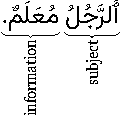
\includegraphics{A-Learners-Grammar-of-Classical-Standard-Arabic_files/figure-latex/unnamed-chunk-35-1.pdf}

Now, as you can see, Arabic does express a word for \enquote{was}. It is the past verb \foreignlanguage{arabic}{کَانَ} \emph{kāna}.
\foreignlanguage{arabic}{کَانَ} is a hollow verb from the root \foreignlanguage{arabic}{«کون»}.
It's resembling verb is \foreignlanguage{arabic}{يَکُونُ} \emph{yakūnu}.
The complete table for this verb for all doer pronouns is given below:

\begin{longtable}[]{@{}lll@{}}
\toprule\noalign{}
Doer pronoun & past verb & resembling verb \\
\midrule\noalign{}
\endhead
\bottomrule\noalign{}
\endlastfoot
he & \foreignlanguage{arabic}{کَانَ} & \foreignlanguage{arabic}{يَکُونُ} \\
she & \foreignlanguage{arabic}{کَانَتْ} & \foreignlanguage{arabic}{تَکُونُ} \\
you\textsubscript{1m} & \foreignlanguage{arabic}{کُنْتَ} & \foreignlanguage{arabic}{تَکُونُ} \\
you\textsubscript{1f} & \foreignlanguage{arabic}{کُنْتِ} & \foreignlanguage{arabic}{تَکُونِينَ} \\
I & \foreignlanguage{arabic}{کُنْتُ} & \foreignlanguage{arabic}{أَکُونُ} \\
they\textsubscript{2m} & \foreignlanguage{arabic}{کَانَا} & \foreignlanguage{arabic}{يَکُونَانِ} \\
they\textsubscript{2f} & \foreignlanguage{arabic}{کَانَتَا} & \foreignlanguage{arabic}{تَکُونَانِ} \\
you\textsubscript{2} & \foreignlanguage{arabic}{کُنْتُمَا} & \foreignlanguage{arabic}{تَکُونَانِ} \\
they\textsubscript{3m} & \foreignlanguage{arabic}{کَانُوا} & \foreignlanguage{arabic}{يَکُونُونَ} \\
they\textsubscript{3f} & \foreignlanguage{arabic}{کُنَّ} & \foreignlanguage{arabic}{يَکُنَّ} \\
you\textsubscript{3m} & \foreignlanguage{arabic}{کُنْتُمْ} & \foreignlanguage{arabic}{تَکُونُونَ} \\
you\textsubscript{3f} & \foreignlanguage{arabic}{کُنْتُنَّ} & \foreignlanguage{arabic}{تَکُنَّ} \\
we & \foreignlanguage{arabic}{کُنَّا} & \foreignlanguage{arabic}{نَکُونُ} \\
\end{longtable}

Like, for other verbs,
the doer of \foreignlanguage{arabic}{کَانَ},
\foreignlanguage{arabic}{ٱلرَّجُلُ}, is in the u-state, and
and its direct doee, \foreignlanguage{arabic}{مُعَلِّمًا}, is in the a-state.

However, unlike most other verbs,
the doer of \foreignlanguage{arabic}{کَانَ},
\foreignlanguage{arabic}{ٱلرَّجُلُ}, is also called its subject
and its direct doee, \foreignlanguage{arabic}{مُعَلِّمًا}, is also called its information.

So a sentence with \foreignlanguage{arabic}{کَانَ} used in this way is a subject-information sentence.
If it begins with \foreignlanguage{arabic}{کَانَ} then it is also a verbal sentence at the same time.

This property also applies to the sisters of \foreignlanguage{arabic}{کَانَ} that we will learn later in this chapter.
Together, these verbs are also called \emph{deficient} verbs, because, besides their doer/subject, they also need an information to complete the meaning of the sentence.
That is, without the information, the sentence is deficient.

\enquote{Is} subject-information sentences can be converted to \enquote{was} subject-information sentences using the verb \foreignlanguage{arabic}{کَانَ}. Here are some examples:

\begin{longtable}[]{@{}
  >{\raggedright\arraybackslash}p{(\columnwidth - 2\tabcolsep) * \real{0.5000}}
  >{\raggedright\arraybackslash}p{(\columnwidth - 2\tabcolsep) * \real{0.5000}}@{}}
\toprule\noalign{}
\begin{minipage}[b]{\linewidth}\raggedright
\enquote{is}
\end{minipage} & \begin{minipage}[b]{\linewidth}\raggedright
\enquote{was}
\end{minipage} \\
\midrule\noalign{}
\endhead
\bottomrule\noalign{}
\endlastfoot
\foreignlanguage{arabic}{زَيْنَبُ جَائِعَةٌ.} & \foreignlanguage{arabic}{کَانَتْ زَيْنَبُ جَائِعَةً.} \\
\enquote{Zaynab is hungry.} & \enquote{Zaynab was hungry.} \\
\foreignlanguage{arabic}{ٱَلْغُلَامُ زَيْدٌ.} & \foreignlanguage{arabic}{کَانَ ٱلْغُلَامُ زَيْدًا.} \\
\enquote{The boy is Zayd.} & \enquote{The boy was Zayd.} \\
\foreignlanguage{arabic}{ٱَلنِّسَاءُ فِي بُيُوتِهِنَّ.} & \foreignlanguage{arabic}{کَانَتْ ٱلنِّسَاءُ فِي بُيُوتِهِنَّ.} \\
\enquote{The women are in their houses.} & \enquote{The women were in their houses.} \\
\foreignlanguage{arabic}{هُمْ مَسْرُورُونَ وَفَرِحُونَ.} & \foreignlanguage{arabic}{کَانُوا مَسْرُورِينَ وَفَرِحِينَ.} \\
\enquote{They\textsubscript{3m} are happy and rejoicing.} & \enquote{They\textsubscript{3m} were happy and rejoicing.} \\
\foreignlanguage{arabic}{أَنَا نَائِمَةٌ.} & \foreignlanguage{arabic}{کُنْتُ نَائِمَةً.} \\
\enquote{I\textsubscript{1f} am sleeping.} & \enquote{I\textsubscript{1f} was sleeping.} \\
\foreignlanguage{arabic}{أَنْتَ لِي أَخٌ.} & \foreignlanguage{arabic}{کُنْتَ لِي أَخًا.} \\
``You\textsubscript{1m} are a brother to me. & ``You\textsubscript{1m} were a brother to me. \\
\end{longtable}

\subsection{\texorpdfstring{Sequence of \foreignlanguage{arabic}{کَانَ}, its subject, and its information}{Sequence of کَانَ, its subject, and its information}}\label{sequence-of-ux643ux627ux646-its-subject-and-its-information}

In sentence word order, the natural sequence is
verb, subject, information.

\foreignlanguage{arabic}{کَانَ زَيْدٌ قَائِمًا.}\\
\enquote{Zayd was standing.}

but we may also, for the same meaning, apply the sequence verb, information, subject:

\foreignlanguage{arabic}{کَانَ قَائِمًا زَيْدٌ.}\\
\enquote{Zayd was standing.}

and also the sequence information, verb, subject:

\foreignlanguage{arabic}{قَائِمًا کَانَ زَيْدٌ.}\\
\enquote{Zayd was standing.}

This last order is common in questions and alternative sentence sentences. For example:

\foreignlanguage{arabic}{أَقَائِمًا کَانَ زَيْدٌ.}\\
\enquote{Was Zayd standing?}

\foreignlanguage{arabic}{ٱُدْعُ زَيْدًا قَائِمًا کَانَ أَوْ جَالِسًا!}\\
\enquote{Call Zayd, be he standing or sitting!}

Sometimes, however, this inversion is impossible because of an indistinguishable state of the two nouns.

For example, in order to express \enquote{My brother was my companion,} we must say:

\foreignlanguage{arabic}{کَانَ أَخِي رَفِيقِي.}\\
\enquote{My brother was my companion.}

This is because, if we invert it, it would naturally mean:

\foreignlanguage{arabic}{کَانَ رَفِيقِي أَخِي.}\\
\enquote{My companion was my brother.}

The following apparent sequence is also possible:

\foreignlanguage{arabic}{زَيْدٌ کَانَ قَائِمًا.}\\
\enquote{Zayd: he was standing.}

But this is actually a topic-comment sentence.
\foreignlanguage{arabic}{زَيْدٌ} is the topic.
And the comment is \foreignlanguage{arabic}{کَانَ قَائِمًا}, which is itself a \foreignlanguage{arabic}{کَانَ} subject-information sentence in the sequence verb, subject, information.
The subject is the hidden pronoun \enquote{he} and the information is \foreignlanguage{arabic}{قَائِمًا}.

\subsection{\texorpdfstring{Plurals of non-rational beings with \foreignlanguage{arabic}{کَانَ}}{Plurals of non-rational beings with کَانَ}}\label{plurals-of-non-rational-beings-with-ux643ux627ux646}

Because \foreignlanguage{arabic}{کَانَ} sentences are subject-information being sentences,
many of the rules that we have learned for subject-information sentences also apply to \foreignlanguage{arabic}{کَانَ} sentences.
One such rule is that when the subject of a sentence is a plural of non-rational beings, and the information is a adjectival noun, then the feminine singular adjectival noun is often used. (See section~\ref{usage-of-plurals-of-non-intelligent-beings}.)
For example:

\foreignlanguage{arabic}{کَانَتِ ٱلْبُيُوتُ صَغِيرَةً.} (typical)\\
\enquote{The houses were small.}

Also allowed, but not as common:\\
\foreignlanguage{arabic}{کَانَتِ ٱلْبُيُوتُ صَغِيرَاتٍ.}\\
\foreignlanguage{arabic}{کَانَتِ ٱلْبُيُوتُ صِغَارًا.}

\foreignlanguage{arabic}{ٱلثِّيرَانُ کَانَتْ ضَخْمَةً.} (typical)\\
\enquote{The bulls were large.}

Also allowed, but not as common:\\
\foreignlanguage{arabic}{ٱلثِّيرَانُ کَانَتْ ضِخَامًا.}\\
\foreignlanguage{arabic}{ٱلثِّيرَانُ کُنَّ ضَخْمَاتٍ.}

\subsection{\texorpdfstring{\foreignlanguage{arabic}{کَانَ} with a separating pronoun}{کَانَ with a separating pronoun}}\label{ux643ux627ux646-with-a-separating-pronoun}

Another rule that applies to subject-information sentences, and that carries over to
\foreignlanguage{arabic}{کَانَ} sentences, is that
when the subject and information are both definite,
then a separating pronoun, which is a detached pronoun that matches the subject, can be inserted between them.
For example,

\foreignlanguage{arabic}{کَانَ ٱلْمُؤْمِنُونَ هُمُ ٱلْفَائِزِينَ.}\\
\enquote{The believers were the winners.}

The separating pronoun \foreignlanguage{arabic}{هُمْ} does not, in this case, serve to disambiguate the information \foreignlanguage{arabic}{ٱلْفَائزِينَ} \enquote{the winners}, from being a describer, as it did in sentences without \foreignlanguage{arabic}{کَانَ} (see section~\ref{subject-information-sentences-separating-pronoun}).
This is because the a-state of \foreignlanguage{arabic}{ٱلْفَائزِينَ} already tells us that it is the information of \foreignlanguage{arabic}{کَانَ}.
If \foreignlanguage{arabic}{ٱلْفَائزِينَ} were a describer of the u-state subject \foreignlanguage{arabic}{ٱَلْمُوْمِنُونَ}, then it too would be in the u-state, not the a-state.
So the separating pronoun serves more, here, to emphasize the subject.

Most of the time, separating pronouns are used in \foreignlanguage{arabic}{کَانَ} sentences when the subject of \foreignlanguage{arabic}{کَانَ} is itself a pronoun. Examples:

\foreignlanguage{arabic}{وَکُنَّا نَحْنُ ٱلْوَارِثِينَ}\\
\enquote{And it is We who were the inheritors} {[}al-Qurʾān 28:58, translation by Saheeh International{]}

\foreignlanguage{arabic}{کُنْتَ أَنْتَ ٱلرَّقِيبَ عَلَيْهِمْ}\\
\enquote{You were the Observer over them} {[}al-Qurʾān 5:117, translation by Saheeh International{]}

Sometimes a pronoun may appear to be a separating pronoun, but actually is not one. Consider, for example, the following sentence:

\foreignlanguage{arabic}{کَانَ ٱلْمُؤْمِنُونَ هُمُ ٱلْفَائِزُونَ.}\\
\enquote{The believers were the winners.}

Note that \foreignlanguage{arabic}{ٱَلْفَائِزُونَ} is in the u-state, so it is not, by itself, the information of \foreignlanguage{arabic}{کَانَ}.
So this is, in fact, a topic-comment sentence.
\foreignlanguage{arabic}{ٱَلْمُوْمِنُونَ} is the topic and the subject of \foreignlanguage{arabic}{کَانَ}.
The information of \foreignlanguage{arabic}{کَانَ} is the comment \foreignlanguage{arabic}{هُمُ ٱلفَائِزُونَ}, which is itself a subject-information sentence with a u-state subject (\foreignlanguage{arabic}{هُمْ}) and a u-state information (\foreignlanguage{arabic}{ٱلْفَائزُونَ}).

\subsection{\texorpdfstring{Negating \foreignlanguage{arabic}{کَانَ}}{Negating کَانَ}}\label{negating-ux643ux627ux646}

Like other past verbs,
the verb \foreignlanguage{arabic}{کَانَ}
may be negated by preceding it with the particle \foreignlanguage{arabic}{مَا}. For example:

\foreignlanguage{arabic}{مَا کَانَ إِبْرَٰهِيمُ يَهُودِيًّۭا وَلَا نَصْرَانِيًّۭا وَلَـٰکِن کَانَ حَنِيفًۭا مُّسْلِمًۭا وَمَا کَانَ مِنَ ٱلْمُشْرِکِينَ}\\
\enquote{Abraham was neither a Jew nor a Christian, but he was one inclining toward truth, a Muslim {[}submitting to Allāh{]}. And he was not of the polytheists.}
(al-Qurʾān 3:67, translation Saheeh International)

A similar meaning may be obtained with the particle \foreignlanguage{arabic}{لَمْ} followed by the
ø-state
resembling verb
\foreignlanguage{arabic}{يَکُنْ}.
This is dealt with in section~\ref{lam-yakun} below.

\subsection{\texorpdfstring{Gender of a pronoun subject of \foreignlanguage{arabic}{کان}}{Gender of a pronoun subject of کان}}\label{gender-of-a-pronoun-subject-of-ux643ux627ux646}

Remember from section~\ref{gender-of-pronoun-subject} that when the subject of a sentence is a pronoun,
then it may optionally either match the gender of the noun it refers to,
or the the gender of the predicate.
This rules carries over to \foreignlanguage{arabic}{کَانَ} subject-information sentences as well. For example:

\foreignlanguage{arabic}{ذَهَبْتُ إِلَى ٱلسُّوقِ فِي ٱلصَّبَاحِ. وَکَانَتْ لِي عَادَةً.}\\
\enquote{I went to the market in the morning. And it was a habit for me.}

\foreignlanguage{arabic}{وَرَکِبُوهُمْ فَکَانَتْ هَزِيمَتَهُمْ}\\
\enquote{And they bore down upon them and it was their defeat.}

Note, how, in the above examples, \foreignlanguage{arabic}{کَانَتْ} has a \foreignlanguage{arabic}{ت} of femininity to match the feminine gender of the information \foreignlanguage{arabic}{عَادَة} \enquote{habit}, and \foreignlanguage{arabic}{هَزِيمَتَهُمْ} \enquote{their defeat}.

\subsection{\texorpdfstring{A pronoun as the information of \foreignlanguage{arabic}{کَانَ}}{A pronoun as the information of کَانَ}}\label{a-pronoun-as-the-information-of-ux643ux627ux646}

TODO

\section{\texorpdfstring{The resembling verb \foreignlanguage{arabic}{يَکُونُ}}{The resembling verb يَکُونُ}}\label{the-resembling-verb-ux64aux643ux648ux646}

The rules related to \foreignlanguage{arabic}{کَانَ}, its subject, and its information, that we have given above apply also to its resembling verb \foreignlanguage{arabic}{يَکُونُ}.

We will now discuss the usages of the specific states of the resembling verb.

\subsection{\texorpdfstring{The u-state resembling verb \foreignlanguage{arabic}{يَکُونُ}}{The u-state resembling verb يَکُونُ}}\label{the-u-state-resembling-verb-ux64aux643ux648ux646}

We have already mentioned that Arabic does not usually express any word for \enquote{is}.
So when, then, is the u-state resembling verb \foreignlanguage{arabic}{يَکُونُ} used?
There are actually a few uses of this verb. We will explain them below:

\subsubsection{\texorpdfstring{\foreignlanguage{arabic}{يَکُونُ} used for habitual \enquote{is}}{يَکُونُ used for habitual ``is''}}\label{ux64aux643ux648ux646-used-for-habitual-is}

Consider the sentence, \enquote{The mother cooks the food.}
The verb \enquote{cooks} implies that the action is habitually done, not necessarily that it is being done at present.
If we wished to say that the action is being done at present, we might instead say, \enquote{The mother \emph{is cooking} the food.}
English maintains this distinction between the present and the habitual for most verbs.
But it does not for ther verb \enquote{is}.
So if we say, \enquote{The sky is blue,} then it can mean both
(i) that the sky is blue at present, or
(ii) that it is habitually blue, not necessarily that it is blue at present.

In Arabic the situation is somewhat different.
Arabic does not usually have a distinction between the present and the habitual for most verbs. So \foreignlanguage{arabic}{تَطْبُخُ الْأُمُّ الطَّعَامَ.} may mean both
(i) that the mother is cooking the food at present, or
(ii) that she habitually does.

But for the verb \enquote{is}, Arabic can distinguish between the present and the habitual.
So if we say \foreignlanguage{arabic}{السَّمَاءُ زَرْقَاءُ}, then this can, in general, mean both
(i) that the sky is blue at present, and
(ii) that it is habitually blue.
If we wish to emphasize the habitual meaning, we may use the resembling verb \foreignlanguage{arabic}{يَکُونُ}, thus:

\foreignlanguage{arabic}{تَکُونُ السَّمَاءُ زَرْقَاءَ.}\\
\enquote{The sky is {[}habitually{]} blue.}

While we call this the
habitual \foreignlanguage{arabic}{يَکُونُ},
it can include a range of meanings, including
continually, recurringly, regularly, typically, generally, often, sometimes, can, may, etc.
Habitual \foreignlanguage{arabic}{يَکُونُ} is negated using \foreignlanguage{arabic}{مَا} or \foreignlanguage{arabic}{لَا}, just like other u-state resembling verbs.

Here are some examples:

\foreignlanguage{arabic}{قَالَ وَمَا الْبِتْعُ وَالْمِزْرُ؟ قُلْتُ شَرَابٌ يَکُونُ مِنَ الْعَسَلِ وَالْمِزْرُ يَکُونُ مِنَ الشَّعِيرِ}\\
``He said: \enquote*{What is mead and beer?} I said: \enquote*{A drink {[}made{]} from honey, and beer is {[}made{]} from barley.}\\
(Part of ḥadīt͡h 5604 from Sunan al-Nisāʾī)

\foreignlanguage{arabic}{يَکُونُ اللِّحَافُ وِسَادَةً وَلَا تَکُونُ الْوِسَادَةُ لِحَافًا.}\\
\enquote{The blanket can be a pillow but the pillow cannot be a blanket.}

\foreignlanguage{arabic}{مَا يَکُونُ الرَّجُلُ صَدِيقَکَ حَتّى يَصْدُقَکَ.}\\
\enquote{A man is not your friend until he is truthful to you.}

\paragraph{\texorpdfstring{\foreignlanguage{arabic}{قَدْ يَکُونُ} for \enquote{may be}}{قَدْ يَکُونُ for ``may be''}}\label{ux642ux62f-ux64aux643ux648ux646-for-may-be}

When the meaning \enquote{may be} is desired, the
the resembling verb
\foreignlanguage{arabic}{يَکُونُ}
may be preceded by the particle \foreignlanguage{arabic}{قَدْ}. For example,

\foreignlanguage{arabic}{قَدْ يَکُونُ الاسْتِهْزَاءُ کُفْرًا.}\\
\enquote{Mocking may be a disbelief.}

\subsubsection{\texorpdfstring{\foreignlanguage{arabic}{يَکُونُ} used for future \enquote{will be}}{يَکُونُ used for future ``will be''}}\label{ux64aux643ux648ux646-used-for-future-will-be}

Another usage of the resembling verb
\foreignlanguage{arabic}{يَکُونُ}
is for the future tense to mean \enquote{will be}.
In this case, it is often preceded by \foreignlanguage{arabic}{سَ} or \foreignlanguage{arabic}{سَوْفَ}.
\foreignlanguage{arabic}{سَ} and \foreignlanguage{arabic}{سَوْفَ} are optional and are commonly dropped, especially when the context indicates the future.
Future \foreignlanguage{arabic}{يَکُونُ}
is negated by \foreignlanguage{arabic}{لَا}.
Here are some examples:

\foreignlanguage{arabic}{فَقَدْ کَذَّبْتُمْ فَسَوْفَ يَکُونُ لِزَامًا}\\
\enquote{For you {[}disbelievers{]} have denied, so it {[}i.e., your denial{]} is going to be adherent.}\\
(al-Qurʾān 25:77, translation Saheeh International)

\foreignlanguage{arabic}{لا يَکونُ اللَّعَّانُونَ شُفَعَاءَ وَلَا شُهَدَاءَ يَومَ القِيَامَةِ}\\
\enquote{The frequent cursers will be neither intercessors nor witnesses {[}on{]} the day of resurrection.}\\
(Ḥadīt͡h 1553 from Riyāḍ al-Ṣāliḥīn, \foreignlanguage{arabic}{يَوْمَ} is in the a-state because it is an adverb of time, see chapter~\ref{adverb-of-time}.)

\foreignlanguage{arabic}{يَوْمَ يَکُونُ ٱلنَّاسُ کَٱلْفَرَاشِ ٱلْمَبْثُوثِ}\\
\enquote{It is the Day when people will be like moths, dispersed,}\\
(al-Qurʾān 101:4, translation Saheeh International)

\subsection{\texorpdfstring{The a-state resembling verb \foreignlanguage{arabic}{يَکُونَ}}{The a-state resembling verb يَکُونَ}}\label{the-a-state-resembling-verb-ux64aux643ux648ux646}

Like a-state resembling verbs in general, \foreignlanguage{arabic}{يَکُونَ} \enquote{be} expresses the meaning of purpose, wish, or expectation. It occurs after the particles
\foreignlanguage{arabic}{أَنْ},
\foreignlanguage{arabic}{لَنْ},
\foreignlanguage{arabic}{لِ},
\foreignlanguage{arabic}{کَيْ},
\foreignlanguage{arabic}{حَتَّىٰ}, and
\foreignlanguage{arabic}{إِذَنْ}.
All this is consistent with what we have learned about a-state resembling verbs in chapter~\ref{a-state-incomplete-action-verbs}.
Here are some examples:

\foreignlanguage{arabic}{نَزَلَ بِهِ ٱلرُّوحُ ٱلْأَمِينُ. عَلَىٰ قَلْبِکَ لِتَکُونَ مِنَ ٱلْمُنذِرِينَ}\\
\enquote{The Trustworthy Spirit {[}i.e., Gabriel{]} has brought it down. Upon your heart, {[}O Muḥammad{]} - that you may be of the warners -}\\
(al-Qurʾān 26:193--194, translation Saheeh International)

\foreignlanguage{arabic}{لَّن يَسْتَنکِفَ ٱلْمَسِيحُ أَن يَکُونَ عَبْدًۭا لِّلَّهِ وَلَا ٱلْمَلَـٰٓئِکَةُ ٱلْمُقَرَّبُونَ}\\
\enquote{Never would the Messiah disdain to be a servant of Allāh, nor would the angels near {[}to Him{]}}\\
(From al-Qurʾān 4:172, translation Saheeh International)

\foreignlanguage{arabic}{أَفَأَنتَ تُکْرِهُ ٱلنَّاسَ حَتَّىٰ يَکُونُوا۟ مُؤْمِنِينَ}\\
\enquote{Then, {[}O Muḥammad{]}, would you compel the people in order that they become believers?}\\
(al-Qurʾān 10:99, translation Saheeh International)

\subsection{\texorpdfstring{The ø-state resembling verb \foreignlanguage{arabic}{يَکُنْ}}{The ø-state resembling verb يَکُنْ}}\label{lam-yakun}

The ø-state resembling verb \foreignlanguage{arabic}{يَکُنْ}
is used consistent with the usage of
ø-state resembling verbs in general.
(See chapter~\ref{0-state-resembling-verbs}.)

For example:

\foreignlanguage{arabic}{وَلْتَکُن مِّنکُمْ أُمَّةٌۭ يَدْعُونَ إِلَى ٱلْخَيْرِ وَيَأْمُرُونَ بِٱلْمَعْرُوفِ وَيَنْهَوْنَ عَنِ ٱلْمُنکَرِ}\\
\enquote{And let there be {[}arising{]} from you a nation inviting to {[}all that is{]} good, enjoining what is right and forbidding what is wrong,1 and those will be the successful.}\\
{[}From al-Qurʾān 3:104, translation by Saheeh International{]}

\foreignlanguage{arabic}{ٱلْحَقُّ مِن رَّبِّکَ فَلَا تَکُن مِّنَ ٱلْمُمْتَرِينَ}\\
\enquote{The truth is from your Lord, so do not be among the doubters.}
{[}From al-Qurʾān 3:60, translation by Saheeh International{]}

\foreignlanguage{arabic}{لَمْ يَکُنِ النَّبِيُّ صلى الله عليه وسلم سَبَّابًا وَلاَ فَحَّاشًا وَلاَ لَعَّانًا}\\
\enquote{The Prophet (ﷺ) was not one who would abuse (others) or say obscene words, or curse (others)}\\
{[}From Ḥadīt͡h in al-Buk͡hārī:6031{]}

\subsubsection{\texorpdfstring{Deletion of \foreignlanguage{arabic}{ن}}{Deletion of ن}}\label{deletion-of-ux646}

The \foreignlanguage{arabic}{ن} may (irregularly) be deleted
for the ø-state resembling verbs that don't have a \foreignlanguage{arabic}{و} before them.
These are:

\begin{itemize}
\tightlist
\item
  \foreignlanguage{arabic}{يَکُنْ}, becomes \foreignlanguage{arabic}{يَکُ}
\item
  \foreignlanguage{arabic}{تَکُنْ}, becomes \foreignlanguage{arabic}{تَکُ}
\item
  \foreignlanguage{arabic}{نَکُنْ}, becomes \foreignlanguage{arabic}{نَکُ}
\item
  \foreignlanguage{arabic}{أَکُنْ}, becomes \foreignlanguage{arabic}{أَکُ}
\end{itemize}

This may only be done when the word following the verb does not begin with a connecting hamzah \foreignlanguage{arabic}{ٱ}.
Examples:

\foreignlanguage{arabic}{وَلَا تَکُ فِى ضَيْقٍۢ مِّمَّا يَمْکُرُونَ}\\
\enquote{and do not be in distress over what they conspire.}\\
{[}From al-Qurʾān 16:127, translation by Saheeh International{]}

\foreignlanguage{arabic}{وَقَدْ خَلَقْتُکَ مِن قَبْلُ وَلَمْ تَکُ شَيْـًۭٔا}\\
\enquote{for I created you before, while you were nothing}\\
{[}From al-Qurʾān 19:9, translation by Saheeh International{]}

But we can't say:

\(\times\) \foreignlanguage{arabic}{لَمْ تَکُ ٱلرَّجُلَ.}

This is because \foreignlanguage{arabic}{ٱلرَّجُل} begins with with a connecting hamzah \foreignlanguage{arabic}{ٱ}. So we have to say instead:

\foreignlanguage{arabic}{لَمْ تَکُنِ ٱلرَّجُلَ.}\\
\enquote{You were not the man.}

\section{\texorpdfstring{The verb of command \foreignlanguage{arabic}{کُنْ}}{The verb of command کُنْ}}\label{kun}

The verb of command \foreignlanguage{arabic}{کُنْ} is used to mean \enquote{Be!}. Examples:

\foreignlanguage{arabic}{قُلْنَا يَـٰنَارُ کُونِى بَرْدًۭا وَسَلَـٰمًا عَلَىٰٓ إِبْرَٰهِيمَ}\\
We {[}i.e., Allāh{]} said, \enquote{O fire, be coolness and safety upon Abraham.}\\
{[}al-Qurʾān 21:69, translation by Saheeh International{]}

\foreignlanguage{arabic}{فَقُلْنَا لَهُمْ کُونُوا۟ قِرَدَةً خَـٰسِـِٔينَ}\\
``and We said to them, \enquote*{Be apes, despised.}\\
{[}From al-Qurʾān 2:65, translation by Saheeh International{]}

The verb of command \foreignlanguage{arabic}{کُنْ} followed by the name of a person in the a-state is used to express one's guessing that the person whom one sees
is the individual named. For example:

\foreignlanguage{arabic}{کُنْ زَيْدًا.}\\
\enquote{I presume that the person approaching is Zayd.}\\
or\\
\enquote{I guess that you are Zayd.}

\section{\texorpdfstring{The complete \foreignlanguage{arabic}{کَانَ}}{The complete کَانَ}}\label{the-complete-ux643ux627ux646}

The verb \foreignlanguage{arabic}{کَانَ} that we have been using so far is called the \emph{deficient}
\foreignlanguage{arabic}{کَانَ}.
It is called so because its meaning is deficient without its information. For example, in the sentence
\foreignlanguage{arabic}{کَانَ زَيْدٌ قَائِمًا} \enquote{Zayd was standing,}
if we remove the information \foreignlanguage{arabic}{قَائِمًا} then the sentence is not complete for the desired meaning.

There is another type of
\foreignlanguage{arabic}{کَانَ}
called the \emph{complete}
\foreignlanguage{arabic}{کَانَ}.
This
\foreignlanguage{arabic}{کَانَ}
does not need an information to complete its meaning.
This
\foreignlanguage{arabic}{کَانَ}
gives the meaning of \enquote{exists}.
In English, we usually express this meaning using \enquote{there was}. For example,

\foreignlanguage{arabic}{کَانَ مَلِکٌ.}\\
\enquote{There was a king.}\\
(literally: \enquote{A king was.})

Note that \foreignlanguage{arabic}{مَلِک} \enquote{king} is in the u-state as the subject.
If it were in the a-state, then it would change the meaning:

\foreignlanguage{arabic}{کَانَ مَلِکًا.}\\
\enquote{He was a king.}

Here are some more examples:

\foreignlanguage{arabic}{کَانَ تَاجِرٌ وَکَانَ لَهُ بَنُونَ.}\\
\enquote{There was a trader, and he had sons.}

Incidentally, as you can see, the past verb of \enquote{have}: \enquote{has} is expressed using \foreignlanguage{arabic}{کَانَ}:

\foreignlanguage{arabic}{کَانَ عِنْدِي کِتَابٌ.}\\
\enquote{I had a book.}\\
(literally: \enquote{A book was for me.})

\foreignlanguage{arabic}{يَکُونُ فِي آخِرِ الزَّمَانِ دَجَّالُونَ کَذَّابُونَ}\\
\enquote{There will be in the end of time charlatan liars}\\
{[}From Ḥadīt͡h in Ṣaḥīḥ Muslim:7{]}

\foreignlanguage{arabic}{إِنَّهَا تَکُونُ الظُّلْمَةُ وَالسَّيْلُ}\\
\enquote{{[}At times there{]} is darkness and flooding}\\
{[}From Ḥadīt͡h in Ṣaḥīḥ al-Buk͡hārī:667{]}

\foreignlanguage{arabic}{لَمْ تَکُنِ ٱلْحَرْبُ.}\\
\enquote{The war didn't occur.}\\
(literally: \enquote{The war was not.})

\section{\texorpdfstring{Time signification of the past verb \foreignlanguage{arabic}{کَانَ}}{Time signification of the past verb کَانَ}}\label{time-signification-of-the-past-verb-ux643ux627ux646}

The general siginification of the past verb
\foreignlanguage{arabic}{کَانَ}
is to indicate a state that existed in the past, and that has possibly ceased.
For example:

\foreignlanguage{arabic}{کَانَ زَيْدٌ قَائِمًا}\\
\enquote{Zayd was standing.}

This statement is regarding Zayd's state in the past and the implication is that he is possibly no longer standing.

This is the most common signification of the past verb
\foreignlanguage{arabic}{کَانَ}
and the one that we have been using so far.
But
\foreignlanguage{arabic}{کَانَ}
is special in that it admits additional significations:

The second signification of
\foreignlanguage{arabic}{کَانَ}
is to indicate a state that, at first, had not yet begun, and which then began and remained, possibly up to the present.
It has, in this sense, the meaning \enquote{became}, \enquote{has become}, or \enquote{happened}. Examples:

\foreignlanguage{arabic}{أَبَىٰ وَٱسْتَکْبَرَ وَکَانَ مِنَ ٱلْکَـٰفِرِينَ}\\
\enquote{He refused and was arrogant and became of the disbelievers.}\\
{[}From al-Qurʾān 2:34, translation by Saheeh International{]}

\foreignlanguage{arabic}{احْتَرَقَ الْخَشَبُ فَکَانَ تُرَابًا.}\\
\enquote{The wood burned and so became dust.}

A third signification of
\foreignlanguage{arabic}{کَانَ}
is
to indicate a state that will be in the future.
For example:

\foreignlanguage{arabic}{وَيَخَافُونَ يَوْمًۭا کَانَ شَرُّهُۥ مُسْتَطِيرًۭا}\\
\enquote{and {[}they{]} fear a Day whose evil will be widespread.}\\
{[}From al-Qurʾān 76:7, translation by Saheeh International{]}

A fourth signification of
\foreignlanguage{arabic}{کَانَ}
is to indicate a state that always existed and will always exist. For example:

\foreignlanguage{arabic}{وَکَانَ ٱللَّهُ غَفُورًۭا رَّحِيمًۢا}\\
\enquote{And ever is Allāh Forgiving and Merciful.}\\
{[}From al-Qurʾān 33:73, translation by Saheeh International{]}

\foreignlanguage{arabic}{وَلَا تَقْرَبُوا۟ ٱلزِّنَىٰٓ ۖ إِنَّهُۥ کَانَ فَـٰحِشَةًۭ وَسَآءَ سَبِيلًۭا}\\
\enquote{And do not approach unlawful sexual intercourse.1 Indeed, it is ever an immorality and is evil as a way.}\\
{[}From al-Qurʾān 17:32, translation by Saheeh International{]}

\section{\texorpdfstring{\foreignlanguage{arabic}{کَانَ} combined with other verbs}{کَانَ combined with other verbs}}\label{ux643ux627ux646-combined-with-other-verbs}

The past verb
\foreignlanguage{arabic}{کَانَ}
and its resembling verb
\foreignlanguage{arabic}{يَکُونُ}
are combined with other verbs to express complex tenses in the past and the future, respectively.
We will explain these combinations below.

\subsection{\texorpdfstring{\foreignlanguage{arabic}{کَانَ} combined with a resembling verb}{کَانَ combined with a resembling verb}}\label{ux643ux627ux646-combined-with-a-resembling-verb}

\foreignlanguage{arabic}{کَانَ}
is combined with a following resembling verb to express that the action of the verb was repeatedly or continually ocurring in the past.
For example:

\foreignlanguage{arabic}{کَانَ زَيْدٌ يَکْتُبُ.}\\
\enquote{Zayd was writing.}\\
or\\
\enquote{Zayd used to write.}\\
or\\
\enquote{Zayd would write.}

This sentence can be analyzed grammatically as a topic-comment sentence.
The subject of
\foreignlanguage{arabic}{کَانَ}
is \foreignlanguage{arabic}{زَيْد} and it is the topic of the sentence.
The information of \foreignlanguage{arabic}{کَانَ} is itself a sentence \foreignlanguage{arabic}{يَکْتُبُ} \enquote{he writes}, and it is the comment of the main sentence.

The order of the subject and the resembling verb can be re-arranged for the same meaning thus:

\foreignlanguage{arabic}{کَانَ يَکْتُبُ زَيْدٌ.}

Now, two grammatical analyses are possible:

\begin{enumerate}
\def\labelenumi{\arabic{enumi}.}
\tightlist
\item
  \foreignlanguage{arabic}{زَيْد} is the doer of \foreignlanguage{arabic}{يَکْتُبُ}, and the subject of \foreignlanguage{arabic}{کَانَ} is a hidden pronoun of the fact.
\item
  \foreignlanguage{arabic}{زَيْد} is the delayed subject of \foreignlanguage{arabic}{کَانَ} and \foreignlanguage{arabic}{يَکْتُبُ} is the information of \foreignlanguage{arabic}{کَانَ}. The doer of \foreignlanguage{arabic}{يَکْتُبُ} is a hidden pronoun.
\end{enumerate}

Either way, the meaning, as we have mentioned, is the same.
Here are some more examples for different types of doers/subjects:

\foreignlanguage{arabic}{کَانَ يَعْبُدُ مُشْرِکُو مَکَّةَ ٱلْأَصْنَامَ.}\\
or\\
\foreignlanguage{arabic}{کَانَ مُشْرِکُو مَکَّةَ يَعْبُدُونَ ٱلْأَصْنَامَ.}\\
\enquote{The polytheists of Makkah used to worship idols.}

\foreignlanguage{arabic}{کَانَتْ تُحِبُّ الصَّدَقَةَ.}\\
\enquote{She used to love {[}to practice{]} charity.}\\
{[}From Ḥadīt͡h in Ṣaḥīḥ al-Buk͡hārī:1420{]}

\foreignlanguage{arabic}{کَانَت تَّأْتِيهِمْ رُسُلُهُم بِٱلْبَيِّنَـٰتِ}\\
\enquote{their messengers used to come to them with clear evidences}\\
{[}From al-Qurʾān 64:6, translation by Saheeh International{]}\\
(Sound plurals, even of rational beings, may be treated as grammatically singular feminine. See section~\ref{sound-plurals-sing-fem}.)

\foreignlanguage{arabic}{کُنْتُ أَلْعَبُ بِالْبَنَاتِ عِنْدَ النَّبِيِّ صلى الله عليه وسلم وَکَانَ لِي صَوَاحِبُ يَلْعَبْنَ مَعِي}\\
\enquote{I used to play with dolls in the presence of the Prophet, and I had companions\textsubscript{f} playing with me.}\\
{[}From Ḥadīt͡h in Ṣaḥīḥ al-Buk͡hārī:6130{]}

Occasionally, the particle \foreignlanguage{arabic}{قَدْ} precedes the combination of \foreignlanguage{arabic}{کَانَ} and the resembling verb. Example:

\foreignlanguage{arabic}{قَالُوا هَذَا قَدْ کَانَ يَکْتُبُ لِمُحَمَّدٍ}\\
\enquote{They said: and said: This {[}person{]} used to transcribe for Muhammad (صلى الله عليه وسلم).}\\
{[}From Ḥadīt͡h in Ṣaḥīḥ Muslim:2781{]}

The following resembling verb may also be an unknown-doer verb. Example:

\foreignlanguage{arabic}{إِنَّ أُنَاسًا کَانُوا يُؤْخَذُونَ بِالْوَحْىِ فِي عَهْدِ رَسُولِ اللَّهِ صلى الله عليه وسلم}\\
\enquote{Indeed people were (sometimes) judged (literally: held) by the {[}revealing of{]} divine inspiration in the lifetime of the Prophet.}\\
{[}From Ḥadīt͡h in Ṣaḥīḥ al-Buk͡hārī:2641{]}

\subsubsection{\texorpdfstring{One \foreignlanguage{arabic}{کَانَ} suffices multiple resembling verbs}{One کَانَ suffices multiple resembling verbs}}\label{one-ux643ux627ux646-suffices-multiple-resembling-verbs}

If the signification of an action ocurring continually in the past applies to more that one resembling verb, then it is sufficient to prefix
\foreignlanguage{arabic}{کَانَ}
to only the first one. Example:

\foreignlanguage{arabic}{کَانَتْ تَعْمَلُ بِيَدِهَا وَتَصَدَّقُ}\\
\enquote{She used to work with her hand and spend (that income) on charity.}
{[}From Ḥadīt͡h in Ṣaḥīḥ Muslim:2452{]}\\
(\foreignlanguage{arabic}{تَتَصَدَّقُ} is abbreviated to \foreignlanguage{arabic}{تَصَدَّقُ}. See section~\ref{form-5-verbs-abbrev}.)

\subsubsection{\texorpdfstring{Negation of \foreignlanguage{arabic}{کَانَ} and a resembling verb}{Negation of کَانَ and a resembling verb}}\label{negation-of-ux643ux627ux646-and-a-resembling-verb}

In order to negate the combination of
\foreignlanguage{arabic}{کَانَ}
and the following resembling verb,
multiple options are available. Using \foreignlanguage{arabic}{يَفْعَلُ} as an example resembling verb, we can have:

\begin{itemize}
\tightlist
\item
  \foreignlanguage{arabic}{مَا کَانَ يَفْعَلُ}
\item
  \foreignlanguage{arabic}{کَانَ لَا يَفْعَلُ}
\item
  \foreignlanguage{arabic}{لَمْ يَکُنْ يَفْعَلُ}
\end{itemize}

Examples:

\foreignlanguage{arabic}{مَا کَانَ أَحَدٌ يَبْدَأُ، أَوْ يَبْدُرُ، ابْنَ عُمَرَ بِالسَّلامِ}\\
\enquote{No one preceded or got ahead of Ibn Ɛumar with (giving) the greeting.}\\
{[}Ḥadīt͡h in al-Adab al-Mufrad:982{]}

\foreignlanguage{arabic}{کَانُوا۟ لَا يَتَنَاهَوْنَ عَن مُّنکَرٍۢ فَعَلُوهُ}\\
\enquote{They used not to prevent one another from wrongdoing that they did.}\\
{[}From al-Qurʾān 5:79, translation by Saheeh International{]}

\foreignlanguage{arabic}{لَمْ يَکُونُوا يَسْأَلُونَ عَنِ الإِسْنَادِ}\\
\enquote{They would not ask about the chains of narration}\\
{[}From Ṣaḥīḥ Muslim:Introduction{]}

\subsubsection{\texorpdfstring{The combination of \foreignlanguage{arabic}{کَانَ} with \foreignlanguage{arabic}{يَکُونُ}}{The combination of کَانَ with يَکُونُ}}\label{the-combination-of-ux643ux627ux646-with-ux64aux643ux648ux646}

Occasionally,
\foreignlanguage{arabic}{کَانَ}
can be combined with its own resembling verb
\foreignlanguage{arabic}{يَکُونُ}
This gives the meaning \enquote{was being} or \enquote{used to be}.
\foreignlanguage{arabic}{يَکُونُ} is, in this combination, often optional and may be dropped for no change in meaning. Examples:

\foreignlanguage{arabic}{کَانَ يَکُونُ فِي مِهْنَةِ أَهْلِهِ}\\
{[}From Ṣaḥīḥ al-Buk͡hārī:676{]}\\
and\\
\foreignlanguage{arabic}{کَانَ فِي مِهْنَةِ أَهْلِهِ}\\
{[}From Ṣaḥīḥ al-Buk͡hārī:6039{]}\\
\enquote{He used to keep himself busy serving his family}

\foreignlanguage{arabic}{قَدْ کَانَ يَکُونُ فِي الأُمَمِ مُحَدَّثُونَ}\\
\enquote{There used to be in the nations inspired persons}\\
{[}From Jāmiɛ al-Tirmid͡hī:2398{]}

\foreignlanguage{arabic}{رِجَالٌ کَانُوا يَکُونُونَ مَعَ ٱلْمُلُوکِ}\\
\enquote{men that used to be with the kings}

\foreignlanguage{arabic}{کَانَ يَکُونُ فِي ٱلْبَيْتِ}\\
\enquote{He used to be in the house.}

\subsubsection{Possible past occurrence}\label{possible-past-occurrence}

Sometimes
\foreignlanguage{arabic}{کَانَ}
is used with a resembling verb to express an action that could have occurred in the past, or should have. Examples:

\foreignlanguage{arabic}{کَانَ يَکُونُ سُوءَ أَدَبٍ.}\\
\enquote{It would have been a misbehavior.}

\foreignlanguage{arabic}{فَقَالَ حُذَيْفَةُ أَنْتَ کُنْتَ تَفْعَلُ ذَلِکَ}\\
\enquote{Ḥud͡hayfah said: \enquote*{You might have done that.}}\\
{[}From Ṣaḥīḥ Muslim:1788{]}

\subsubsection{\texorpdfstring{Omission of \foreignlanguage{arabic}{کَانَ}}{Omission of کَانَ}}\label{omission-of-ux643ux627ux646}

If one or more past verbs precedes the resembling verb
or if the context indicates that the action was occurring in the past, then
\foreignlanguage{arabic}{کَانَ}
can be omitted, and the resembling verb is used by itself. For example:

\foreignlanguage{arabic}{قُلْ فَلِمَ تَقْتُلُونَ أَنۢبِيَآءَ ٱللَّهِ مِن قَبْلُ}\\
\enquote{Say,}Then why did you kill the prophets of Allāh before''\\
{[}From al-Qurʾān 2:91, translation by Saheeh International{]}\\
(No \foreignlanguage{arabic}{کُنْتُمْ} before \foreignlanguage{arabic}{تَقْتُلُونَ}.)

\foreignlanguage{arabic}{وَٱتَّبَعُوا۟ مَا تَتْلُوا۟ ٱلشَّيَـٰطِينُ عَلَىٰ مُلْکِ سُلَيْمَـٰنَ ۖ}\\
\enquote{And they followed {[}instead{]} what the devils had recited during the reign of Solomon}\\
{[}From al-Qurʾān 2:102, translation by Saheeh International{]}\\
(No \foreignlanguage{arabic}{کَانَتْ} before \foreignlanguage{arabic}{تَتْلُو}.)

\subsubsection{\texorpdfstring{\foreignlanguage{arabic}{کَانَ} followed by a doer or doee verbal-noun instead of a resembling verb}{کَانَ followed by a doer or doee verbal-noun instead of a resembling verb}}\label{ux643ux627ux646-followed-by-a-doer-or-doee-verbal-noun-instead-of-a-resembling-verb}

Instead of a resembling verb after \foreignlanguage{arabic}{کَانَ}, its doer or doee verbal noun may be used instead.
And this can give the effect of a state of being rather than an action being done.
For example:

\foreignlanguage{arabic}{کَانَ سَاکِنًا فِي ٱلْمَدِينَةِ.}\\
\enquote{He was dwelling in the city.}

\foreignlanguage{arabic}{کَانَتِ ٱلْعُصِيُّ مَرْکُوزَةً فِي ٱلْأَرْضِ.}\\
\enquote{The staffs were sticking in the ground.}\\
(\foreignlanguage{arabic}{کَانَتْ تُرْکَزُ} would imply that they were being stuck.)

When the verbal noun refers to an action taking place in the future, the idea of futurity is transferred to a past time. For example:

\foreignlanguage{arabic}{أَمْرٌ کَانَ مَفْعُولًا}\\
\enquote{a matter which was to be done}

\subsection{\texorpdfstring{\foreignlanguage{arabic}{کَانَ} combined with a past verb}{کَانَ combined with a past verb}}\label{ux643ux627ux646-combined-with-a-past-verb}

\foreignlanguage{arabic}{کَانَ}
is combined with a following past verb to denote
an action completed prior to some past (specified or implied) point in time.
Example:

\foreignlanguage{arabic}{مَاتَ ٱلرَّشِيدُ بِطُوسَ وَکَانَ خَرَجَ إِلَىٰ خُرَاسَانَ لِمُحَارَبَةِ رَافِعِ بْنِ ٱللَّيْثِ.}\\
\enquote{al-Ras͡hīd died at Ṭūs after (literally: and) he had set out for K͡hurāsān to combat Rāfiɛ ibn al-Layt͡h.}

The particle \foreignlanguage{arabic}{قَدْ} is often used when
\foreignlanguage{arabic}{کَانَ} is combined with a past verb.
\foreignlanguage{arabic}{قَدْ}
may be placed either between
\foreignlanguage{arabic}{کَانَ}
and the following past verb, or before
\foreignlanguage{arabic}{کَانَ}.
Examples:

\foreignlanguage{arabic}{کُنْتُ قَدْ رَبَّيْتُ جَارِيَةً}\\
\enquote{I had brought up a girl}

\foreignlanguage{arabic}{قَدْ کَانَتْ فَرَغَتْ مِنْ عَمَلِهَا.}\\
\enquote{She had been done with her work.}

When their are multiple past verbs, and one (or more) of them occurred
farther in the past than the others, it is indicated with
\foreignlanguage{arabic}{قَدْ},
the others having merely
\foreignlanguage{arabic}{کَانَ}.
We re-use a previous example here and extend it:

\foreignlanguage{arabic}{مَاتَ ٱلرَّشِيدُ بِطُوسَ وَکَانَ خَرَجَ إِلَىٰ خُرَاسَانَ لِمُحَارَبَةِ رَافِعِ بْنِ ٱللَّيْثِ.}\\
\foreignlanguage{arabic}{وَکَانَ رَافِعٌ هَـٰذَا قَدْ خَرَجَ وَخَلَعَ ٱلطَّاعَةَ وَتَغَلَّبَ عَلَىٰ سَمَرْقَنْدَ.}\\
\enquote{al-Ras͡hīd died at Ṭūs after he had set out for K͡hurāsān to combat Rāfiɛ ibn al-Layt͡h.
And this Rāfiɛ had already rebelled and cast off his allegiance and taken forcible posession of Samarqand.}\\
(Note how
\foreignlanguage{arabic}{قَدْ}
is only used before
Rāfiɛ's action of rebelling.)

\subsubsection{Negation}\label{negation-1}

This combination may, again, be negated in multiple ways. Examples:

\foreignlanguage{arabic}{لاَ يَأْتِي ابْنَ آدَمَ النَّذْرُ بِشَىْءٍ لَمْ يَکُنْ قَدْ قَدَّرْتُهُ}\\
\enquote{Vowing does not bring to the son of Adam anything I have not already written in his fate,}\\
{[}From Ṣaḥīḥ al-Buk͡hārī:6609{]}

\foreignlanguage{arabic}{وَدِدْتُ أَنِّي لَمْ أَکُنْ خَرَجْتُ الْعَامَ}\\
\enquote{I wish I had not come out (for Ḥajj) this year}\\
{[}From Sunan Abī Dawūd:1778{]}

\foreignlanguage{arabic}{وَمَا کَانَ قَدْ أَتَاهَا بِشَيْءٍ}\\
\enquote{And he had not brought her anything}

\subsection{\texorpdfstring{\foreignlanguage{arabic}{يَکُونُ} combined with a past verb}{يَکُونُ combined with a past verb}}\label{ux64aux643ux648ux646-combined-with-a-past-verb}

The resembling verb
\foreignlanguage{arabic}{يَکُونُ}
is compined with a past verb (often with an interposed \foreignlanguage{arabic}{قَدْ})
to express that the action is conceived of having been completed in the future.
Examples:

\foreignlanguage{arabic}{يَکُونُ قَدْ وَجَبَ عَلَيْکَ صَدَقَةٌ}\\
\enquote{Charity will have been incumbent upon you}\\
{[}From Mis͡hkāt al-Maṣābīḥ:1793{]}

\foreignlanguage{arabic}{فَلْنَأْخُذْهُ فَنَکُونُ قَدْ أَخَْذْنَا عِوَضًا}\\
\enquote{Let us take him for (then) we will have taken a substitute}

\subsubsection{\texorpdfstring{a-state \foreignlanguage{arabic}{يَکُونَ} combined with a past verb}{a-state يَکُونَ combined with a past verb}}\label{a-state-ux64aux643ux648ux646-combined-with-a-past-verb}

An a-state \foreignlanguage{arabic}{يَکُونَ} is combined with a past verb
to express being in a state of an action having occurred
or that might have occurred. For example:

\foreignlanguage{arabic}{خَافَ أَنْ يَکُونَ قَدْ خَطَأَ}\\
\enquote{He feared that he could have erred.}

\foreignlanguage{arabic}{وَيَجُوزُ أَنْ يَکُونُوا قَدْ سُبِقُوا}\\
\enquote{And that they might have been preceded is possible}

\foreignlanguage{arabic}{يَشْطَرِطُ فِي ٱلنَّائِبِ أَنْ يَکُونَ قَدْ حَجَّ عَنْ نَفْسِهِ}\\
\enquote{It is conditional for the deputy that he be in as state of already having performed the Ḥajj for himself.}

\subsection{\texorpdfstring{Verb of command \foreignlanguage{arabic}{کُنْ} combined with a resembling verb}{Verb of command کُنْ combined with a resembling verb}}\label{verb-of-command-ux643ux646-combined-with-a-resembling-verb}

Ocassionally,
the verb of command \foreignlanguage{arabic}{کُنْ} is combined with a resembling verb, thus:

\foreignlanguage{arabic}{کُنْ أَنْتَ تُکَلِّمُهُمْ}\\
\enquote{You be speaking to them!}

\section{\texorpdfstring{\foreignlanguage{arabic}{کَانَ} with the \foreignlanguage{arabic}{ل} of denial}{کَانَ with the ل of denial}}\label{ux643ux627ux646-with-the-ux644-of-denial}

One special use of
\foreignlanguage{arabic}{کَانَ}
is what is termed the
\foreignlanguage{arabic}{ل}
\emph{of denial}.
This is a negative
\foreignlanguage{arabic}{کَانَ}
(either
\foreignlanguage{arabic}{مَا کَانَ}
or
\foreignlanguage{arabic}{لَمْ يَکُنْ} with the appropriate suffixes or prefixes for the subject)
followed by \foreignlanguage{arabic}{لِ}
and then an a-state resembling verb.
This expresses the meaning of:

\begin{enumerate}
\def\labelenumi{\roman{enumi}.}
\tightlist
\item
  to deny being the one to do something, or
\item
  to deny going to do something
\end{enumerate}

Here are some examples:

\foreignlanguage{arabic}{لَمْ تَکُنْ زَيْنَبُ لِتَضْرِبَ وَلَدَهَا}\\
\enquote{Zaynab was not one to beat her child.}\\
or\\
\enquote{Zaynab was not going to beat her child.}

\foreignlanguage{arabic}{وَمَا کَانَ ٱللَّهُ لِيُعَذِّبَهُمْ وَأَنتَ فِيهِمْ ۚ}\\
\enquote{But Allāh would not punish them while you, {[}O Muḥammad{]}, are among them}\\
{[}From al-Qurʾān 8:33, translation by Saheeh International{]}

\foreignlanguage{arabic}{فَقَالَ أَتَخْشَيْنَ أَنْ أَقْتُلَهُ مَا کُنْتُ لأَفْعَلَ ذَلِکَ}\\
\enquote{He said: Do you fear that I shall kill him ? I am not going to do that.}\\
{[}From Sunan Abī Dawūd:3112{]}

\foreignlanguage{arabic}{قَالَ لَمْ أَکُنْ لأَفْعَلَ}\\
\enquote{He said: I was not going to do that.}
{[}From Sunan Ibn Mājah:1503{]}

\section{\texorpdfstring{\foreignlanguage{arabic}{کَانَ} with the \foreignlanguage{arabic}{ل} of deserving}{کَانَ with the ل of deserving}}\label{ux643ux627ux646-with-the-ux644-of-deserving}

Closely related, yet distinct from,
the use of
\foreignlanguage{arabic}{کَانَ} with the \foreignlanguage{arabic}{ل} of denial
(above)
is
the use of
\foreignlanguage{arabic}{کَانَ} with a \foreignlanguage{arabic}{ل} that signifies deserving, behooving, appropriateness, or possibility.
This is, again, a negative
\foreignlanguage{arabic}{کَانَ}
followed by the preposition \foreignlanguage{arabic}{لِ}
and a following i-state noun,
and then \foreignlanguage{arabic}{أَنْ} followed by an a-state resembling verb.
This signifies that the action of the verb does not behoove, or is not appropriate or desrving or possibly for the person denoted by the noun after \foreignlanguage{arabic}{لِ}.
For example:

\foreignlanguage{arabic}{فَأَنۢبَتْنَا بِهِۦ حَدَآئِقَ ذَاتَ بَهْجَةٍۢ مَّا کَانَ لَکُمْ أَن تُنۢبِتُوا۟ شَجَرَهَآ ۗ}\\
\enquote{causing to grow thereby gardens of joyful beauty which you could not {[}otherwise{]} have grown the trees thereof}\\
{[}From al-Qurʾān 27:60, translation by Saheeh International{]}

\foreignlanguage{arabic}{مَا کَانَ لِبَشَرٍ أَن يُؤْتِيَهُ ٱللَّهُ ٱلْکِتَـٰبَ وَٱلْحُکْمَ وَٱلنُّبُوَّةَ ثُمَّ يَقُولَ لِلنَّاسِ کُونُوا۟ عِبَادًۭا لِّى مِن دُونِ ٱللَّهِ}\\
\enquote{It is not for a human {[}prophet{]}1 that Allāh should give him the Scripture2 and authority and prophethood and then he would say to the people,}Be servants to me rather than Allāh,``\,''\\
{[}From al-Qurʾān 3:79, translation by Saheeh International{]}

\foreignlanguage{arabic}{قَالَ أَبُو بَکْرٍ مَا کَانَ لاِبْنِ أَبِي قُحَافَةَ أَنْ يُصَلِّيَ بَيْنَ يَدَىْ رَسُولِ اللَّهِ صلى الله عليه وسلم}\\
\enquote{Abu Bakr said ; it was not befitting for the son of Abu Quhafah (Abu Bakr) to lead the prayer in the presence of the Messenger of Allah (ﷺ)}\\
{[}From Sunan Abī Dawūd:940{]}

\chapter{\texorpdfstring{\foreignlanguage{arabic}{إِنَّ} and its sisters}{إِنَّ and its sisters}}\label{inna-and-its-sisters}

\section{Introduction}\label{introduction-23}

In the basic subject-information sentence, both the subject and the information are in the u-state. For example:


\includegraphics{A-Learners-Grammar-of-Classical-Standard-Arabic_files/figure-latex/unnamed-chunk-36-1.pdf}

\enquote{This man is a teacher.}

In the above sentence both the subject \foreignlanguage{arabic}{ٱَلرَّجُلَ} \enquote{the man}, and the information \foreignlanguage{arabic}{مُعَلِّمٌ} \enquote{a teacher} are in the u-state. In this chapter we will study a family of particles, called
\foreignlanguage{arabic}{إِنَّ} and its sisters,
that modify the subject-information sentence by placing the subject in the a-state instead of the u-state. For example,

\foreignlanguage{arabic}{إِنَّ ٱلرَّجُلَ مُعَلِّمٌ.}\\
\emph{ʾinna -rrajula muɛallimun.}\\
\enquote{Indeed the man is a teacher.}

Note how, in the above example, the subject \foreignlanguage{arabic}{ٱَلرَّجُلَ} \enquote{the man} is now in the a-state. The information \foreignlanguage{arabic}{مُعَلِّمٌ} \enquote{a teacher} remains in the u-state.

The particles constituting the family of
\foreignlanguage{arabic}{إِنَّ} and its sisters
are:

\begin{enumerate}
\def\labelenumi{\arabic{enumi}.}
\tightlist
\item
  \foreignlanguage{arabic}{إِنَّ} \emph{ʾinna} \vphantom{\huge J}
\item
  \foreignlanguage{arabic}{أَنَّ} \emph{ʾanna} \vphantom{\huge J}
\item
  \foreignlanguage{arabic}{کَأَنَّ} \emph{kaʾanna} \vphantom{\huge J}
\item
  \foreignlanguage{arabic}{لَـٰکِنَّ} \emph{lākinna} \vphantom{\huge J}
\item
  \foreignlanguage{arabic}{لَيْتَ} \emph{layta} \vphantom{\huge J}
\item
  \foreignlanguage{arabic}{لَعَلَّ} \emph{laɛalla} \vphantom{\huge J}
\end{enumerate}

We shall now study each of these particles.

\section{\texorpdfstring{\foreignlanguage{arabic}{إِنَّ} \emph{ʾinna}}{إِنَّ ʾinna}}\label{ux625ux646-einna}

\foreignlanguage{arabic}{إِنَّ} \emph{ʾinna} is used to begin independent sentences. It has an emphatic meaning, as if the speaker is asserting the information about the subject. It is often translated into English as \enquote{indeed} or \enquote{verily}, but it is also often left untranslated.

\foreignlanguage{arabic}{إِنَّ} \emph{ʾinna} is only used to begin subject-information sentences. Verbal sentences cannot be introduced by \foreignlanguage{arabic}{إِنَّ} \emph{ʾinna} directly. (Later, in section~\ref{damiir-al-shan}, we shall see how to overcome this restriction.). For example,

\foreignlanguage{arabic}{إِنَّ ٱلدِّينَ عِنْدَ ٱللَّـٰهِ ٱلْإِسْلَامُ.}\\
\emph{ʾinna -ddīna ɛinda -llāhi -lʾislāmu.}\\
\enquote{Indeed, the religion in the sight of Allāh is Islām.} (Qurʾān~3:19, trans. Saheeh International)

\foreignlanguage{arabic}{إِنَّ} \emph{ʾinna}
may be preceded by other particles like \foreignlanguage{arabic}{وَ} \enquote{and}, \foreignlanguage{arabic}{فَ} \enquote{so}, and \foreignlanguage{arabic}{ثُمَّ} \enquote{then}. For example,

\foreignlanguage{arabic}{ٱُطْلُبِ ٱلْعِلْمَ ٱلنَّافِعَ. فَإِنَّ طَلَبَ ٱلْعِلْمَ ٱلنَّافِعَ عَمَلٌ صَالِحٌ. وَإِنَّ تَرْکَهُ غَفْلَةٌ.}
\enquote{Seek the useful knowledge. For indeed the seeking of the useful knowledge is a good deed. And indeed leaving it is a negligence.}

The subject of
\foreignlanguage{arabic}{إِنَّ} \emph{ʾinna}
may be a noun phrase, in which case, any describers or replacements of the subject are also in the a-state. Examples:

\foreignlanguage{arabic}{إِنَّ هَـٰؤُلَاءِ ٱلرِّجَالَ ٱلْکِرَامَ أَصْدِقَائِي.}\\
\enquote{Indeed these noble men are my friends.}

\foreignlanguage{arabic}{إِنَّ} \emph{ʾinna} may have multiple subjects, each in the a-state, separated by \foreignlanguage{arabic}{وَ}. Example,

\foreignlanguage{arabic}{إِنَّ ٱلْمُسْلِمِينَ وَٱلْمُسْلِمَاتِ يَعْبُدُونَ ٱللَّـٰهَ.}\\
\enquote{Indeed the Muslim men and Muslim women worship Allāh.}

If the information of the first subject has been mentioned before the second subject, then the second subject may optionally be in the a-state or the u-state. For example:

\foreignlanguage{arabic}{إِنَّ زَيْدًا جَالِسٌ وَعَمْرًا.}\\
or\\
\foreignlanguage{arabic}{إِنَّ زَيْدًا جَالِسٌ وَعَمْرٌو.}\\
\enquote{Indeed Zayd is sitting and Ɛamr {[}as well{]}.}

\foreignlanguage{arabic}{إِنَّ هَـٰذَا ٱلْکِتَابَ لِي وَذَ ٰلِکَ ٱلْکِتَابَ لَکَ.}\\
or\\
\foreignlanguage{arabic}{إِنَّ هَـٰذَا ٱلْکِتَابَ لِي وَذَ ٰلِکَ ٱلْکِتَاکُ لَکَ.}\\
\enquote{Indeed this book is for me and that book is for you.}

\foreignlanguage{arabic}{إِنَّ} \emph{ʾinna} may be used to begin sentences with an indefinite subject. For example,

\foreignlanguage{arabic}{إِنَّ مَلِکًا مِنَ ٱلْهِنْدِ کَتَبَ إِلَىٰ أَحَدِ وُزَرَائِهِ.}\\
\enquote{Indeed a king from India wrote to one of his ministers.}

Note that in all the above examples that
\foreignlanguage{arabic}{إِنَّ} \emph{ʾinna} is only used to begin subject-information sentences. Verbal sentences cannot be introduced by \foreignlanguage{arabic}{إِنَّ} \emph{ʾinna} directly. (Later, in section~\ref{damiir-al-shan}, we shall see how to overcome this restriction.).
By default, the subject of \foreignlanguage{arabic}{إِنَّ} \emph{ʾinna} must directly follow it with no intervening words or particles. The only exception is when the information consists of a prepositional or adverbial phrase, it is then allowed to precede the subject. The subject, in any case, shall be in the a-state. For example,

\foreignlanguage{arabic}{إِنَّ فِي ٱلْبَيْتِ رَجُلًا.}\\
\enquote{Indeed, in the house, is a man.}

\foreignlanguage{arabic}{إِنَّ تَحْتَ ٱلشَّجَرَةِ کَنْزًا ثَمِينًا.}\\
\enquote{Indeed, under the tree, is a precious treasure.}

This reverse order is permitted even when the subject is definite. For example,

\foreignlanguage{arabic}{إِنَّ مَعَکَ صَاحِبَکَ.}\\
\enquote{Indeed, with you, is \emph{your companion}.}

This puts the logical accent on the subject \foreignlanguage{arabic}{صَاحِبَکَ} \enquote{your companion}. If the subject is placed first then this puts the logical accent on the information:

\foreignlanguage{arabic}{إِنَّ صَاحِبَکَ مَعَکَ.}\\
\enquote{Indeed your companion is \emph{with} you.}

If the subject contains a pronoun that refers to a noun in the information then the information must precede the subject. For example,

\foreignlanguage{arabic}{إِنَّ فِي ٱلْمَصْنَعِ عُمَّالَهُ.}\\
\enquote{Indeed, in the factory, are its workers.}

\foreignlanguage{arabic}{إِنَّ أَمَامَ ٱلدَّارِ حَارِسَهَا.}\\
\enquote{Indeed, in front of the door, is its guard.}

\subsection{Pronoun subjects}\label{pronoun-subjects}

The subject of \foreignlanguage{arabic}{إِنَّ} may be a pronoun instead of a noun. For this the attached pronouns are used. For example,

\foreignlanguage{arabic}{لَا تَقْطَعْ تِلْکَ ٱلشَّجَرَةَ فَإِنَّهَا ظَلِيلَةٌ.}\\
\enquote{Don't cut that tree, for it is shady.}

\foreignlanguage{arabic}{إِنَّکُمَا صَدِيقَايَ.}\\
\enquote{You\textsubscript{2} are my friends.}

The speaker pronouns, both singular and plural, may optionally keep or drop their \foreignlanguage{arabic}{ن}.
So for the singular speaker pronoun both \foreignlanguage{arabic}{إِنَّنِي} \emph{ʾinnanī} and \foreignlanguage{arabic}{إِنِّي} \emph{ʾinnī} may be used.
And for the plural speaker pronoun both \foreignlanguage{arabic}{إِنَّنَا} \emph{ʾinnanā} and \foreignlanguage{arabic}{إِنَّا} \emph{ʾinnā} may be used.
Examples:

\foreignlanguage{arabic}{إِنِّي مُسْلِمٌ.}\\
or\\
\foreignlanguage{arabic}{إِنَّنِي مُسْلِمٌ.}\\
\enquote{Indeed I am a Muslim.}

\foreignlanguage{arabic}{إِنَّنَا کَاتِبُو هَـٰذَا ٱلْکِتَابَ.}\\
or\\
\foreignlanguage{arabic}{إِنَّا کَاتِبُو هَـٰذَا ٱلْکِتَابَ.}\\
\enquote{Indeed we are the writers of this book.}

TODO: Multiple pronoun subjects: \foreignlanguage{arabic}{إِنِّ وَ إِيَّاکَ \ldots{}}

\foreignlanguage{arabic}{إِنَّ} with the speaker pronouns are often used with doer verbal nouns to signify that the speaker intends to to the action of the verb. For example,

\foreignlanguage{arabic}{إِنِّي ذَاهِبٌ إِلَىٰ ٱلْمَسْجِدِ.}\\
\enquote{I'm going to the mosque.}

We also mentioned this point in section~\ref{doer-verbal-noun-for-intended-future-action}.

\subsection{\texorpdfstring{\foreignlanguage{arabic}{إِنَّ} \emph{ʾinna} with a strengthening \foreignlanguage{arabic}{لَ}}{إِنَّ ʾinna with a strengthening لَ}}\label{inna-strengthening-la}

The strengthening particle \foreignlanguage{arabic}{لَ} adds extra emphasis and may optionally be used between the subject of \foreignlanguage{arabic}{إِنَّ} and its information.
If the subject occurs first (as is the default) then \foreignlanguage{arabic}{لَ} is connected to and placed directly before the information. For example:

\foreignlanguage{arabic}{إِنَّ زَيْدًا لَقَائِمٌ.}\\
\enquote{Indeed Zayd is definitely standing.}

If the information precedes the subject, then then \foreignlanguage{arabic}{لَ} is connected to and placed directly before the subject. For example:

\foreignlanguage{arabic}{إِنَّ فِي ٱلْبَيْتِ لَرَجُلًا.}\\
\enquote{Indeed, in the house, is definitely a man.}

The strengthening particle \foreignlanguage{arabic}{لَ} is only used with \foreignlanguage{arabic}{إِنَّ} and not for any of its other sisters
(\foreignlanguage{arabic}{إِنَّ},
\foreignlanguage{arabic}{أَنَّ},
\foreignlanguage{arabic}{کَأَنَّ},
\foreignlanguage{arabic}{لَـٰکِنَّ},
\foreignlanguage{arabic}{لَيْتَ}, and
\foreignlanguage{arabic}{لَعَلَّ}).

\subsection{\texorpdfstring{Commonality of rules for \foreignlanguage{arabic}{إِنَّ} and its sisters}{Commonality of rules for إِنَّ and its sisters}}\label{commonality-of-rules-for-ux625ux646-and-its-sisters}

Unless otherwise noted, the rules we have presented above for
\foreignlanguage{arabic}{إِنَّ},
for example, the subject being in the a-state, the order of the subject and the predicate, the use of attached pronouns for the subject, etc.,
apply also to its other sisters.

The strengthening particle \foreignlanguage{arabic}{لَ}, as mentioned above, is only used with \foreignlanguage{arabic}{إِنَّ} and not for any of its other sisters.

\section{\texorpdfstring{\foreignlanguage{arabic}{أَنَّ} \emph{ʾanna}}{أَنَّ ʾanna}}\label{ux623ux646-eanna}

The particle
\foreignlanguage{arabic}{أَنَّ} \emph{ʾanna}
can be translated as \enquote{that}.
It is similar to \foreignlanguage{arabic}{إِنَّ} in that it is asserts the information about the subject.
But
\foreignlanguage{arabic}{أَنَّ} is different from \foreignlanguage{arabic}{إِنَّ} in that \foreignlanguage{arabic}{إِنَّ}, its subject, and its information together constitute a complete sentence.
Whereas
the
\foreignlanguage{arabic}{أَنَّ}
clause
(\foreignlanguage{arabic}{أَنَّ}
, its subject, and its information together) does not constitute a complete sentence. For example, consider the expression:

\foreignlanguage{arabic}{زَيْدٌ صَادِقٌ.}\\
\enquote{Zayd is truthful.}

This is a complete sentence. But if we add
\foreignlanguage{arabic}{أَنَّ} \enquote{that} to its beginning, it no longer remains a complete sentence:

\foreignlanguage{arabic}{أَنَّ زَيْدًا صَادِقٌ}\\
\enquote{that Zayd is truthful}

We need to additional words, external to the
\foreignlanguage{arabic}{أَنَّ}
clause
to complete the sentence. We will see examples of this below.

\subsection{\texorpdfstring{The \foreignlanguage{arabic}{أَنَّ} clause in place of the direct doee}{The أَنَّ clause in place of the direct doee}}\label{the-ux623ux646-clause-in-place-of-the-direct-doee}


\includegraphics{A-Learners-Grammar-of-Classical-Standard-Arabic_files/figure-latex/unnamed-chunk-37-1.pdf}

\enquote{I know that Zayd is truthful.}

Note how, in the example above the
\foreignlanguage{arabic}{أَنَّ}
clause
(\foreignlanguage{arabic}{أَنَّ زَيْدًا صَادِقٌ})
has occupied the place of the direct doee of the verb \foreignlanguage{arabic}{أَعْلَمُ}.

In a similar manner,
\foreignlanguage{arabic}{أَنَّ}
clauses can be placed where one would expect other noun positions, such as: a subject, an information, a doer, and more. Here are some examples:

\subsection{\texorpdfstring{The \foreignlanguage{arabic}{أَنَّ} clause in place of the doer}{The أَنَّ clause in place of the doer}}\label{the-ux623ux646-clause-in-place-of-the-doer}

Example:

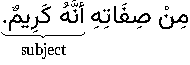
\includegraphics{A-Learners-Grammar-of-Classical-Standard-Arabic_files/figure-latex/unnamed-chunk-38-1.pdf}

\enquote{That you are sick has reached me.} (\enquote{It has reached me that you are sick.})

\subsection{\texorpdfstring{The \foreignlanguage{arabic}{أَنَّ} clause in place of the subject}{The أَنَّ clause in place of the subject}}\label{the-ux623ux646-clause-in-place-of-the-subject}

Example (with information before subject in sentence word order):


\includegraphics{A-Learners-Grammar-of-Classical-Standard-Arabic_files/figure-latex/unnamed-chunk-39-1.pdf}

\enquote{From his characteristeics is that he is noble.}

\subsection{\texorpdfstring{The \foreignlanguage{arabic}{أَنَّ} clause in place of the information}{The أَنَّ clause in place of the information}}\label{the-ux623ux646-clause-in-place-of-the-information}

Example:


\includegraphics{A-Learners-Grammar-of-Classical-Standard-Arabic_files/figure-latex/unnamed-chunk-40-1.pdf}

\enquote{The truth is that he went.}

\subsection{\texorpdfstring{\foreignlanguage{arabic}{أَنَّ} with \foreignlanguage{arabic}{کَانَ}}{أَنَّ with کَانَ}}\label{ux623ux646-with-ux643ux627ux646}

As you know, \foreignlanguage{arabic}{کَانَ}'s doer is also its subject, and its doee is also its information.
The \foreignlanguage{arabic}{أَنَّ} clause can occur in either the subject or the information of \foreignlanguage{arabic}{کَنَ}.
For example, the \foreignlanguage{arabic}{أَنَّ} clause as the information:


\includegraphics{A-Learners-Grammar-of-Classical-Standard-Arabic_files/figure-latex/unnamed-chunk-41-1.pdf}

\enquote{The matter was that he didn't do his obligation.}

Now, the \foreignlanguage{arabic}{أَنَّ} clause as the subject:

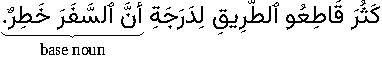
\includegraphics{A-Learners-Grammar-of-Classical-Standard-Arabic_files/figure-latex/unnamed-chunk-42-1.pdf}

\enquote{That he didn't do his obligation was the matter.}

Note that in the latter case, the information precedes the subject.

\subsection{\texorpdfstring{The \foreignlanguage{arabic}{أَنَّ} clause in place of an i-state noun}{The أَنَّ clause in place of an i-state noun}}\label{the-ux623ux646-clause-in-place-of-an-i-state-noun}

The \foreignlanguage{arabic}{أَنَّ} clause can occur in place of an i-state base noun in an annexation. Example:

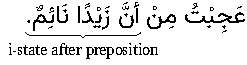
\includegraphics{A-Learners-Grammar-of-Classical-Standard-Arabic_files/figure-latex/unnamed-chunk-43-1.pdf}

\enquote{The highway robbers (literally: the cutters of the way) have increased to the degree that the journey is dangerous.}

The \foreignlanguage{arabic}{أَنَّ} clause can occur in place of an i-state noun directly following a preposition. Example:

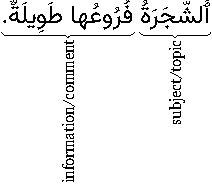
\includegraphics{A-Learners-Grammar-of-Classical-Standard-Arabic_files/figure-latex/unnamed-chunk-44-1.pdf}

\enquote{I wondered at that Zayd is asleep.}

\subsubsection{\texorpdfstring{Optionally deleting the preposition directlt before an \foreignlanguage{arabic}{أَنَّ} clause}{Optionally deleting the preposition directlt before an أَنَّ clause}}\label{optionally-deleting-the-preposition-directlt-before-an-ux623ux646-clause}

If an
\foreignlanguage{arabic}{أَنَّ} clause
directly follows a preposition, it is permissible to optionally delete the preposition as long as the meaning remains clear.
So the previous example can be expressed without the preposition \foreignlanguage{arabic}{مِنْ} with the same meaning:

\foreignlanguage{arabic}{عَجِبْتُ أَنَّ زَيْدًا نَائِمٌ.}\\
\enquote{I wondered at that Zayd is asleep.}

\subsubsection{\texorpdfstring{\foreignlanguage{arabic}{لِأَنَّ} \enquote{because}}{لِأَنَّ ``because''}}\label{ux644ux623ux646-because}

The combination of the preposition \foreignlanguage{arabic}{لِ} \enquote{for} and \foreignlanguage{arabic}{أَنَّ} is used to mean \enquote{because}. For example,

\foreignlanguage{arabic}{أَکَلْتُ ٱلطَّعَامَ لِأَنَّنِي کُنْتُ جَائِعًا.}\\
\enquote{I ate the food because I was hungry.}

\subsection{\texorpdfstring{Equivalence of the \foreignlanguage{arabic}{أَنَّ} clause with a verbal noun of doing}{Equivalence of the أَنَّ clause with a verbal noun of doing}}\label{equivalence-of-the-ux623ux646-clause-with-a-verbal-noun-of-doing}

As a matter of grammatical theory, the
\foreignlanguage{arabic}{أَنَّ} clause, i.e.~(\foreignlanguage{arabic}{أَنَّ} itself, its subject, and its information) is considered equivalent to a verbal noun of doing (typically in an annexation, and possibly with a doee as well). It is this equivalalence that allows it to thake the place of a doer, direct doee, and the other categories we have given above.
For instance, consider the example:

\foreignlanguage{arabic}{عَجِبْتُ مِنْ أَنَّ زَيْدًا ذَهَب.}\\
\enquote{I wondered at that Zayd went.}

Here, the clause
\foreignlanguage{arabic}{أَنَّ زَيْدًا ذَهَب}
is equivalent to the verbal noun phrase \foreignlanguage{arabic}{ذَهَابِ زَيْدٍ} \enquote{Zayd's going}. So the grammatically equivalent sentence with this verbal noun phrase is:

\foreignlanguage{arabic}{عَجِبْتُ مِنْ ذَهَابِ زَيْدٍ.}\\
\enquote{I wondered at Zayd's going.}

Similarly, in the example,

\foreignlanguage{arabic}{مِنْ صِفَاتِهِ أَنَّهُ کَرِيمٌ.}\\
\enquote{From his characteristics is that he is generous.}

the clause
\foreignlanguage{arabic}{أَنَّهُ کَرِيمٌ}
is equivalent to the verbal noun phrase \foreignlanguage{arabic}{کَرَامَتِهِ} \enquote{his generosity}. So the grammatically equivalent sentence with this verbal noun phrase is:

\foreignlanguage{arabic}{کَرَامَتِهِ مِنْ صِفَاتِهِ.}\\
\enquote{His generosity is from his characteristics.}

This grammatical equivalence is more a matter of theory than of practical usefulness to us.
And you have seen this grammatical equivalence before with \foreignlanguage{arabic}{أَنْ} and a-state incomplete action verbs in chanpter~\ref{a-state-incomplete-action-verbs-verbal-noun}.

\section{\texorpdfstring{\foreignlanguage{arabic}{کَأَنَّ} \emph{kaʾanna}}{کَأَنَّ kaʾanna}}\label{ux643ux623ux646-kaeanna}

\foreignlanguage{arabic}{کَأَنَّ} \emph{kaʾanna}
may be translated as \enquote{{[}It is{]} as if}.
It is actually simply the preposition \foreignlanguage{arabic}{کَ} \enquote{like} attached to \foreignlanguage{arabic}{أَنَّ}. But it is treated separately because, unlike \foreignlanguage{arabic}{أَنَّ},
\foreignlanguage{arabic}{کَأَنَّ} \emph{kaʾanna}, its subject, and its information constitute a complete sentence. For example,

\foreignlanguage{arabic}{کَأَنَّ ٱلْأُمُّ مَدْرَسَةٌ.}\\
\enquote{{[}It is{]} as if the mother is a school.}

TODO: add more info

\section{\texorpdfstring{\foreignlanguage{arabic}{لَـٰکِنَّ} \emph{lākinna}}{لَـٰکِنَّ lākinna}}\label{ux644ux640ux643ux646-lakinna}

TODO

\section{\texorpdfstring{\foreignlanguage{arabic}{لَيْتَ} \emph{layta}}{لَيْتَ layta}}\label{ux644ux64aux62a-layta}

TODO

\section{\texorpdfstring{\foreignlanguage{arabic}{لَعَلَّ} \emph{laɛalla}}{لَعَلَّ laɛalla}}\label{ux644ux639ux644-laealla}

TODO

\section{Topic-comment sentences and the pronoun of the fact}\label{topic-comment-sentences-and-the-pronoun-of-the-fact}

\subsection{Topic-comment sentences}\label{topic-comment-sentences}

There is a sub-type of subject-information sentence called a topic-comment sentence. Here is an example:

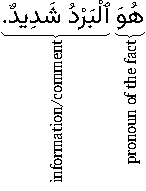
\includegraphics{A-Learners-Grammar-of-Classical-Standard-Arabic_files/figure-latex/unnamed-chunk-45-1.pdf}

\enquote{The tree: its branches are long.}

In these kinds of sentences, the subject introduces a topic, and the information is itself a sentence which comments on the topic/subject.
We have, in fact, already seen sentences like this in section~\ref{past-verbs-order-of-words}, when we take a verbal sentence and convert it to a subject-information sentence. This is the example we discussed there:

\foreignlanguage{arabic}{ٱَلرَّجُلُ کَتَبَ کِتَابًا.}\\
\enquote{The man: he wrote a book.}

\subsubsection{The linker pronoun}\label{the-linker-pronoun}

A topic-comment sentence typically requires a pronoun in the comment that links back to the comment.
In the example
\foreignlanguage{arabic}{ٱَلشَّجَرَةُفُرُوعُهَا طَوِيلَةٌ.}, the attached pronoun \foreignlanguage{arabic}{هَا} \enquote{it} in \foreignlanguage{arabic}{فُرُوعُهَا} \enquote{its tree} is the linker pronoun that links back to the topic \foreignlanguage{arabic}{ٱَلشَّجَرَةُ} \enquote{the tree}.

Similarly, in the example
\foreignlanguage{arabic}{ٱَلرَّجُلُ کَتَبَ کِتَابًا.}
the linker pronoun is the invisible doer pronoun \enquote{he} of the verb \foreignlanguage{arabic}{کَتَبَ} \enquote{he wrote} that links back to the topic \foreignlanguage{arabic}{ٱَلرَّجُلُ} \enquote{the man}.

\subsubsection{\texorpdfstring{Topic-comment sentences with \foreignlanguage{arabic}{إِنَّ} and its sisters}{Topic-comment sentences with إِنَّ and its sisters}}\label{topic-comment-sentences-with-ux625ux646-and-its-sisters}

\foreignlanguage{arabic}{إِنَّ} and its sisters are very often used in topic-comment sentences. (With \foreignlanguage{arabic}{أَنَّ} it is, as usual, an incomplete sentence.) Here are some examples:

\foreignlanguage{arabic}{إِنَّ زَيْدًا لَهُ أَخٌ وَأُخْتٌ.}\\
\enquote{Indeed Zayd: he has a brother and sister.}

\foreignlanguage{arabic}{ٱِعْلَمْ أَنَّ ٱلْعِلْمَ حُصُولُهُ يَتَطَلَّبُ جُهْدًا.}\\
\enquote{Know that knowledge: its obtaining requires effort.}

\subsubsection{Topic-comment sentences with a pronoun topic}\label{topic-comment-sentences-with-a-pronoun-topic}

The topic, in a topic-comment sentence, is frequently a pronoun. For example,

\foreignlanguage{arabic}{أَنَا ٱسْمِي زَيْدٌ.}\\
\enquote{I: my name is Zayd.}

\foreignlanguage{arabic}{أَکَلْتُ ٱلطَّعَامَ لَـٰکِنَّکَ لَمْ تَأْکُلْ.}\\
\enquote{I ate the food but you: you didn't eat.}

\subsection{The pronoun of the fact}\label{the-pronoun-of-the-fact}

Mostly, pronouns are used in place of nouns when it is already known to whom the noun refers to. So if you say:

\foreignlanguage{arabic}{أَنَا ٱسْمِي زَيْدٌ.}\\
\enquote{I: my name is Zayd.}

the pronoun \foreignlanguage{arabic}{أَنَا} \enquote{I} refers to the speaker, who is known.

There is a special pronoun, called the \emph{pronoun of the fact} that begins topic-comment sentences. This pronoun does not refer to any previously known entity, but rather refers to the comment that follows it. It is sometimes translated as \enquote{the fact is} but is often left untranslated. Here is an example:

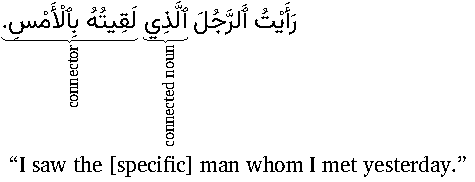
\includegraphics{A-Learners-Grammar-of-Classical-Standard-Arabic_files/figure-latex/unnamed-chunk-46-1.pdf}

\enquote{The fact is: the cold is intense.}

This pronoun is usually the singular masculine pronoun (as above) but it is also sometimes the singular feminine pronoun \foreignlanguage{arabic}{هِيَ}.
It is typically used with statements of import, to which the speaker wishes to draw attention.
The comment does not contain a linker pronoun because the whole comment refers back to the topic.
The pronoun of the fact is frequently used with \foreignlanguage{arabic}{إِنَّ} and its sisters.
Here are some examples:

\foreignlanguage{arabic}{إِنَّهُ لَا يُفْلِحُ ٱلْکَافِرُونَ.}\\
\enquote{Indeed, the disbelievers will not succeed.}\\
(Qurʾān 23:117, trans. Saheeh International)

Sometimes, one can choose between using the pronoun of the fact and a pronoun matching the participant resulting in different emphasis. For example,

\foreignlanguage{arabic}{إِنِّهُ هُمُ ٱلْفَاعِلُونَ}\\
\enquote{Indeed, the fact is: they are the doers.}

\foreignlanguage{arabic}{إِنِّهُمْ هُمُ ٱلْفَاعِلُونَ}\\
\enquote{Indeed, \emph{they} are the doers.}

\section{\texorpdfstring{The lightened versions \foreignlanguage{arabic}{إِنْ}, \foreignlanguage{arabic}{أَنْ}, \foreignlanguage{arabic}{کَأَنْ}, and \foreignlanguage{arabic}{لَـٰکِنْ}}{The lightened versions إِنْ, أَنْ, کَأَنْ, and لَـٰکِنْ}}\label{the-lightened-versions-ux625ux646-ux623ux646-ux643ux623ux646-and-ux644ux640ux643ux646}

The particles \foreignlanguage{arabic}{إِنَّ}, \foreignlanguage{arabic}{أَنَّ}, \foreignlanguage{arabic}{کَأَنَّ}, and \foreignlanguage{arabic}{لَـٰکِنَّ}, because of the doubled \foreignlanguage{arabic}{نّ} are considered \emph{heavy}.
There exist \emph{lightened} versions of these particles that are:
\foreignlanguage{arabic}{إِنْ}, \foreignlanguage{arabic}{أَنْ}, \foreignlanguage{arabic}{کَأَنْ}, and \foreignlanguage{arabic}{لَـٰکِنْ}.
These lightened versions have similar meanings to their heavy counterparts but they have somewhat different rules. We will discuss them below.
In terms of their usage
\foreignlanguage{arabic}{إِنْ} and
\foreignlanguage{arabic}{کَأَنْ} are not very commonly used except in the Qurʾān, poetry, and other rhetorical texts.
\foreignlanguage{arabic}{أَنْ} and
\foreignlanguage{arabic}{لَـٰکِنْ}
are relatively more common.

\subsection{\texorpdfstring{The lightened \foreignlanguage{arabic}{إِنْ}}{The lightened إِنْ}}\label{the-lightened-ux625ux646}

The lightened
\foreignlanguage{arabic}{إِنْ}
is used in two different ways.
In the more common way, the subject is not put in the a-state but is rather in the u-state.
However, the strengthening \foreignlanguage{arabic}{لَ} (see section~\ref{inna-strengthening-la} above), that was optional with the heavy \foreignlanguage{arabic}{إِنَّ}, is now mandatory with the lightened \foreignlanguage{arabic}{إِنْ}. For example,

\foreignlanguage{arabic}{إِنْ زَيْدٌ لَمُسْلِمٌ.}\\
\enquote{Indeed Zayd is a Muslim.}

The other notable difference between
the lightened \foreignlanguage{arabic}{إِنْ}
and
the heavy \foreignlanguage{arabic}{إِنَّ}
is that
the heavy \foreignlanguage{arabic}{إِنَّ} is only used to introduce subject-information sentences.
The lightened \foreignlanguage{arabic}{إِنْ},
however, can be used to introduce verbal sentences, but only those that begin with the verbs:
\foreignlanguage{arabic}{کَانَ} and its sisters,
\foreignlanguage{arabic}{کَادَ} and its sisters, and
\foreignlanguage{arabic}{ظَنَّ} and its sisters.
For example,

\foreignlanguage{arabic}{قَرَأْتُ ٱلْکِتَابَ وَإِنْ کَانَ ٱلْکِتَابُ لَجَيِّدًا.}\\
\enquote{I read the book and indeed the book was good.}

The second, less common way, of using
the lightened \foreignlanguage{arabic}{إِنْ}
is following the same rules as the
the heavy \foreignlanguage{arabic}{إِنَّ}.
Where the subject is in the a-state and the use of the strengthening \foreignlanguage{arabic}{لَ} is optional. For example,

\foreignlanguage{arabic}{إِنْ زَيْدًا مُسْلِمٌ.}\\
\enquote{Indeed Zayd is a Muslim.}

\subsection{\texorpdfstring{The lightened \foreignlanguage{arabic}{أَنْ}}{The lightened أَنْ}}\label{lightened-an}

As we know, the heavy \foreignlanguage{arabic}{أَنَّ} is an emphatic particle and is frequently used with the pronoun of the fact, thus:

\foreignlanguage{arabic}{أَعْلَمُ أَنَّهُ ٱلْبَرْدُ شَدِيدٌ.}\\
\enquote{I know that the fact is: the cold is intense.}

When we wish not to use much emphasis, we may replace
the heavy \foreignlanguage{arabic}{أَنَّ} along with its following pronoun of the fact (\foreignlanguage{arabic}{أَنَّهُ}/\foreignlanguage{arabic}{أَنَّهَا}) with
a lightened \foreignlanguage{arabic}{أَنْ}, thus:

\foreignlanguage{arabic}{أَعْلَمُ أَنِ ٱلْبَرْدُ شَدِيدٌ.}\\
\enquote{I know that the cold is intense.}

Note that
the lightened \foreignlanguage{arabic}{أَنْ} replaces
\foreignlanguage{arabic}{أَنَّهُ},
which is the combination of
heavy \foreignlanguage{arabic}{أَنَّ} \emph{and} the pronoun of the fact \foreignlanguage{arabic}{هُ}.
So the pronoun of the fact (\foreignlanguage{arabic}{هُ}) does not appear with
the lightened \foreignlanguage{arabic}{أَنْ}.

In the above example,
the lightened \foreignlanguage{arabic}{أَنْ}
introduces a comment which is a subject-predicate sentence.
But the more common use of
the lightened \foreignlanguage{arabic}{أَنْ}
is to introduce comments that are verbal sentences.

When the comment of the
lightened \foreignlanguage{arabic}{أَنْ}
is a verbal sentence, then it is preferred to separate the verb from \foreignlanguage{arabic}{أَنْ} with one of the following:

\begin{enumerate}
\def\labelenumi{\arabic{enumi}.}
\item
  \foreignlanguage{arabic}{قَدْ}. Example:

  \foreignlanguage{arabic}{أَظُنُّ أَنْ قَدْ غَرَبَتِ ٱلشَّمْسُ.}\\
  \enquote{I think that the sun has set.}
\item
  \foreignlanguage{arabic}{سَ} or \foreignlanguage{arabic}{سَوْفَ}. Example:

  \foreignlanguage{arabic}{أَعْلَمُ أَنْ سَيَذْهَبُ.}\\
  \enquote{I know that he will go.}
\item
  A negative particle like \foreignlanguage{arabic}{لَا}, \foreignlanguage{arabic}{لَنْ}, or \foreignlanguage{arabic}{لَمْ}.

  \foreignlanguage{arabic}{أَعْلَمُ أَنْ لَا يَذْهَبُ.}\\
  \enquote{I know that he does/will not go.}

  Note that, in writing, we have not combined the lightened \foreignlanguage{arabic}{أَنْ} and \foreignlanguage{arabic}{لَا} to form \foreignlanguage{arabic}{أَلَّا}, as is done for the a-state-verbal \foreignlanguage{arabic}{أَنْ} (for example: \foreignlanguage{arabic}{أَلَّا يَذْهَبَ} \enquote{that he not go}) in chapter~\ref{chapter-a-state-incomplete-action-verbs}. This distinction in spelling is not obligatory, but some authorities recommend it. In any case, they are both pronounced the same: \emph{ʾallā}.

  More examples:

  \foreignlanguage{arabic}{أَعْلَمُ أَنْ لَنْ يَذْهَبَ.}\\
  \enquote{I know that he shall not go.}

  \foreignlanguage{arabic}{أَعْلَمُ أَنْ لَمْ يَذْهَبْ.}\\
  \enquote{I know that he did not go.}

  Note that the \foreignlanguage{arabic}{لَنْ} and \foreignlanguage{arabic}{لَمْ}, even when after the lightened \foreignlanguage{arabic}{أَنْ}, change the state of the following incomplete-action verb to the a-state and ø-state respectively.
\item
  The conditional particle \foreignlanguage{arabic}{لَوْ}. We will study conditional sentences in chapter~\ref{conditional-sentences}. TODO: add example.
\end{enumerate}

Rigid verbs like \foreignlanguage{arabic}{لَيْسَ} and verbs expressing supplications are exempted from needing to be separated from the lightened \foreignlanguage{arabic}{أَنْ}. Example:

\foreignlanguage{arabic}{ظَنَنْتُ أَنْ لَيْسَ ٱلْبَرْدُ شَدِيدًا.}\\
\enquote{I thought that the cold is not intense.}

\subsubsection{\texorpdfstring{Distinguishing between the lightened \foreignlanguage{arabic}{أَنْ} and the a-state-verbal \foreignlanguage{arabic}{أَنْ}}{Distinguishing between the lightened أَنْ and the a-state-verbal أَنْ}}\label{distinguishing-between-the-lightened-ux623ux646-and-the-a-state-verbal-ux623ux646}

Although they are similar in meaning,
care must be taken to distinguish between this lightened \foreignlanguage{arabic}{أَنْ} and the a-state-verbal \foreignlanguage{arabic}{أَنْ}
(that we learned in chapter~\ref{chapter-a-state-incomplete-action-verbs}),
The a-state-verbal \foreignlanguage{arabic}{أَنْ} puts the following incomplete action verb in the a-state.
Whereas the incomplete action verb directly after the lightened \foreignlanguage{arabic}{أَنْ} remains in the u-state.
The following guidelines can help to distinguish between these two \foreignlanguage{arabic}{أَنْ}s:

\begin{itemize}
\item
  If the verb before \foreignlanguage{arabic}{أَنْ} signifies certainty then only \foreignlanguage{arabic}{أَنَّ} and its lightened version \foreignlanguage{arabic}{أَنْ} is used. For example,

  \foreignlanguage{arabic}{أَعْلَمُ أَنْ قَدْ ذَهَبَ وَأَنْ سَيَرْجِعُ.}\\
  \enquote{I know that he has gone and that he will return.}
\item
  If the verb before \foreignlanguage{arabic}{أَنْ} signifies wanting, hoping, or expecting, then the \foreignlanguage{arabic}{أَنْ} puts the following verb in the a-state. For example,

  \foreignlanguage{arabic}{أَطْمَعُ أَلَّا يَذْهَبَ.}\\
  \enquote{I hope that he not go.}

  Note that the verb \foreignlanguage{arabic}{يَذْهَبَ} is in the a-state.
\item
  If the verb before \foreignlanguage{arabic}{أَنْ} reflects a view of something going to occur, and signifies neither certainty nor expectation, but rather doubt or neutrality, then either of the \foreignlanguage{arabic}{أَنْ}s may be used, depending on the intended meaning. Such verbs include \foreignlanguage{arabic}{ظَنَّ يَظُنُّ} \enquote{to think} and \foreignlanguage{arabic}{حَسِبَ يَحْسِبُ} \enquote{to deem}. For example,

  a-state-verbal \foreignlanguage{arabic}{أَنْ}:\\
  \foreignlanguage{arabic}{ظَنَنْتُ أَنْ يَرْجِعَ.}\\
  \enquote{I thought that he should return.}

  lightened \foreignlanguage{arabic}{أَنْ}:\\
  \foreignlanguage{arabic}{ظَنَنْتُ أَنْ يَرْجِعُ.}\\
  \enquote{I thought that he will return.}
\item
  If the verb before \foreignlanguage{arabic}{أَنْ} does not reflect a view of something going to occur then the \foreignlanguage{arabic}{أَنْ} is typically the a-state-verbal \foreignlanguage{arabic}{أَنْ}. For example,

  \foreignlanguage{arabic}{سَرَّنِي أَنْ تَنْجَحَ}\\
  \enquote{That you succeed {[}will have{]} gladdened me.}

  Remember from chapter~\ref{chapter-a-state-incomplete-action-verbs}), that the a-state-verbal \foreignlanguage{arabic}{أَنْ} can occur with completed-action verbs as well. Example:

  \foreignlanguage{arabic}{سَرَّنِي أَنْ نَجَحْتَ}\\
  \enquote{That you have succeeded {[}has{]} gladdened me.}
\end{itemize}

\subsection{\texorpdfstring{The lightened \foreignlanguage{arabic}{کَأَنْ}}{The lightened کَأَنْ}}\label{the-lightened-ux643ux623ux646}

The lightened \foreignlanguage{arabic}{کَأَنْ} is similar to the lightened \foreignlanguage{arabic}{أَنْ} in that it introduces a topic-comment sentence and the topic is usually a deleted pronoun of the fact. For example,

\foreignlanguage{arabic}{کَأَنْ ٱلْبَرْدُ ذَهَبَ.}\\
\enquote{{[}It is{]} as if the cold has gone.}

Also similar to the lightened \foreignlanguage{arabic}{أَنْ}, the lightened \foreignlanguage{arabic}{کَأَنْ} may introduce a verbal sentence but it must be separated from \foreignlanguage{arabic}{کَأَنْ} by either \foreignlanguage{arabic}{قَدْ} or \foreignlanguage{arabic}{لَمْ}. For example,

\foreignlanguage{arabic}{ذَهَبَ کَأَنْ لَمْ يَسْمَعْ.}\\
\enquote{He went as if he did not hear.}

\subsection{\texorpdfstring{The lightened \foreignlanguage{arabic}{لَـٰکِنْ}}{The lightened لَـٰکِنْ}}\label{the-lightened-ux644ux640ux643ux646}

The lightened \foreignlanguage{arabic}{لَـٰکِنْ} has the same meaning as the heavy \foreignlanguage{arabic}{لَـٰکِنَّ} but it has no grammatical effect on the word or sentence after it. It may introduce either subject-information or verbal sentences. For example,

\foreignlanguage{arabic}{نَجَحَ زَيْدٌ لَـٰکِنْ صَدِيقُهُ لَمْ يَنْجَحْ.}\\
\enquote{Zayd succeeded but his friend did not succeed.}

\appendix


\chapter{Rules for writing hamzah}\label{hamzarules}

\section{Seats of hamzah}\label{seats-of-hamzah}

Hamzah is written in four different ways:

\begin{enumerate}
\def\labelenumi{\arabic{enumi}.}
\tightlist
\item
  Seated on an alif: {\tradarab{أ}} or {\tradarab{إ}}
\item
  Seated on an wāw: {\tradarab{ؤ}}
\item
  Seated on an yāʾ: {\tradarab{ئ}}
\item
  Unseated: {\tradarab{ء}}
\end{enumerate}

Here are some of notes about writing hamzah in the above four methods:

\begin{itemize}
\item
  When unseated hamzah comes between two letters that are joined, then it is written above the line that joins them, for example: {\tradarab{خَطِيءَة}} \emph{k͡haṭīʾah}. In this word, the yāʾ {\tradarab{ي}} joins to the \emph{tāʾ marbūṭah} {\tradarab{ة}}.

  As a special case, when unseated hamza comes between joined lām and alif ({\tradarab{لا}}), then it is positioned between them thus: {\tradarab{لءا}}. (In most cases, this is replaced with {\tradarab{لآ}} as we will explain in the next point below.) And this is different from hamzah on the alif following the lām: {\tradarab{لأ}}.
\item
  When unseated hamzah is followed by an alif: {\tradarab{ءا}}, the combination of hamzah and alif is usually written as {\tradarab{آ}} as a convention. Examples: {\tradarab{آمَنَ}} \emph{ʾāmana}, {\tradarab{ظَمْآن}} \emph{ḍ͡hamʾān}, {\tradarab{شَنَآن}} \emph{s͡hanaʾān}. However, when the alif is a suffix or part of a suffix, or the hamzah is doubled, or there is an alif before the hamzah then we will write {\tradarab{ءا}}, not {\tradarab{آ}}. Examples: {\tradarab{شَيْءَانِ}} \emph{s͡hayʾāni}, {\tradarab{سَءَّال}} \emph{saʾʾāl}, {\tradarab{قِرَاءَات}} \emph{qirāʾāt}.
\item
  When hamzah is seated on alif, if it has an \emph{i}-mark, it is written below the alif: {\tradarab{إِ}}. Otherwise, it is written above the alif: {\tradarab{أَ}}, {\tradarab{أُ}}, {\tradarab{أْ}}.
\item
  When hamzah is seated on yāʾ {\tradarab{ئ}} the dots of the yāʾ are no longer written. Here's how it will appear in different positions:

  \begin{longtable}[]{@{}llll@{}}
  \toprule\noalign{}
  Isolated & End & Middle & Beginnning \\
  \midrule\noalign{}
  \endhead
  \bottomrule\noalign{}
  \endlastfoot
  {\tradarab{ئ}} & {\tradarab{ـئ}} & {\tradarab{ـئـ}} & {\tradarab{ئـ}} \\
  \end{longtable}

  Note that hamzah is seated on yāʾ in the middle position {\tradarab{ـئـ}} is different from unseated hamzah between two joining letters {\tradarab{ـءـ}}.
\end{itemize}

So how do we know when to write hamzah unseated and when seated? And how do we choose between its three different seats? There are a set of rules that we need to follow in order to correctly write hamzah.

\section{Rules for determining the seat of hamzah}\label{rules-for-determining-the-seat-of-hamzah}

\subsection{Without prefixes and suffixes}\label{without-prefixes-and-suffixes}

We will first learn how to determine the seat of hamzah for a word
without any prefix or suffix.

Hamzah can occur in three positions in a word:

\begin{enumerate}
\def\labelenumi{\arabic{enumi}.}
\tightlist
\item
  At the beginning of the word
\item
  In the middle of the word
\item
  At the end of the word
\end{enumerate}

We will treat each of these positions below.

\subsubsection{At the beginning of the word}\label{at-the-beginning-of-the-word}

When hamzah occurs in the beginning of a word, then:

\begin{enumerate}
\def\labelenumi{\alph{enumi}.}
\tightlist
\item
  If the hamzah carries a long-\emph{ā} vowel, it is written unseated followed by an alif and written as {\tradarab{آ}}, for example {\tradarab{آمَنَ}} \emph{ʾāmana}.
\item
  If the hamzah carries any other vowel, it is written seated on an alif, and is marked with the appropriated vowel mark, for example {\tradarab{أَسْلَمَ}} \emph{ʾaslama}, {\tradarab{أُرِيدُ}} \emph{ʾurīdu}, {\tradarab{إِسْلَام}} \emph{ʾislām}, {\tradarab{إِيمَان}} \emph{ʾīmān}, {\tradarab{أُوخِذَ}} \emph{ʾūk͡hid͡ha}.
\end{enumerate}

\subsubsection{In the middle of the word}\label{in-the-middle-of-the-word}

The most general case is when hamzah is in the middle of a word.

Arabic has three short vowels, three long vowels, two semi-vowels, and a zero-vowel indicated by a ø-mark {\tradarab{◌ْ}}. Each of these has an order of precedence and a hamzah seat, that we have shown in the table below:

\begin{longtable}[]{@{}lll@{}}
\toprule\noalign{}
Precedence & Vowel & Seated hamzah \\
\midrule\noalign{}
\endhead
\bottomrule\noalign{}
\endlastfoot
1. & \emph{ī}/\emph{ay} & {\tradarab{ء}} \\
2. & \emph{i} & {\tradarab{ئ}} \\
3. & \emph{ū}/\emph{aw} & {\tradarab{ء}} \\
4. & \emph{u} & {\tradarab{ؤ}} \\
5. & \emph{ā} & {\tradarab{ء}} \\
6. & \emph{a} & {\tradarab{أ}} \\
7. & {\tradarab{◌ْ}} & {\tradarab{ء}} \\
\end{longtable}

\textbf{Main rule:} Disregard any doubling mark {\tradarab{◌ّ}}. Consider the vowel on the consonant before the hamzah and the \emph{shortened} vowel on the hamzah itself. Determine which of the two vowels wins by being higher in precedence in the above table. The winning vowel's seat will be the seat of the hamzah.

\textbf{Sub-rule:} If the main rule determines that hamzah is to be seated on alif, and there is a long \emph{ā} vowel on the hamzah using an alif, then hamzah shall be unseated. And the combination of {\tradarab{ءَا}} will usually be written as {\tradarab{آ}}.

Examples:

\begin{longtable}[]{@{}
  >{\raggedright\arraybackslash}p{(\columnwidth - 8\tabcolsep) * \real{0.3158}}
  >{\raggedright\arraybackslash}p{(\columnwidth - 8\tabcolsep) * \real{0.1053}}
  >{\raggedright\arraybackslash}p{(\columnwidth - 8\tabcolsep) * \real{0.1053}}
  >{\raggedright\arraybackslash}p{(\columnwidth - 8\tabcolsep) * \real{0.1053}}
  >{\raggedright\arraybackslash}p{(\columnwidth - 8\tabcolsep) * \real{0.3684}}@{}}
\toprule\noalign{}
\begin{minipage}[b]{\linewidth}\raggedright
Word
\end{minipage} & \begin{minipage}[b]{\linewidth}\raggedright
Vowel on consonant before hamzah
\end{minipage} & \begin{minipage}[b]{\linewidth}\raggedright
Shortened vowel on hamzah
\end{minipage} & \begin{minipage}[b]{\linewidth}\raggedright
Winning vowel
\end{minipage} & \begin{minipage}[b]{\linewidth}\raggedright
Seated hamzah
\end{minipage} \\
\midrule\noalign{}
\endhead
\bottomrule\noalign{}
\endlastfoot
\vphantom{\huge J} {\tradarab{هَيْءَة}} \emph{hayʾah} & \emph{ay} & \emph{a} & \emph{ay} & {\tradarab{ء}} \\
\vphantom{\huge J} {\tradarab{خَطِيءَة}} \emph{k͡haṭīʾah} & \emph{ī} & \emph{a} & \emph{ī} & {\tradarab{ء}} \\
\vphantom{\huge J} {\tradarab{اسْتِيءَاس}} \emph{ʾistīʾās} & \emph{ī} & \emph{a} & \emph{ī} & {\tradarab{ء}} (Exception: {\tradarab{ءَا}} is not written as {\tradarab{آ}} when the preceding vowel is \emph{ī}.) \\
\vphantom{\huge J} {\tradarab{تَوْءَم}} \emph{tawʾam} & \emph{aw} & \emph{a} & \emph{aw} & {\tradarab{ء}} \\
\vphantom{\huge J} {\tradarab{سَائِل}} \emph{sāʾil} & \emph{ā} & \emph{i} & \emph{i} & {\tradarab{ئ}} \\
\vphantom{\huge J} {\tradarab{تَسَاؤُل}} \emph{tasāʾul} & \emph{ā} & \emph{u} & \emph{u} & {\tradarab{ؤ}} \\
\vphantom{\huge J} {\tradarab{تَسَاءَلَ}} \emph{tasāʾala} & \emph{ā} & \emph{a} & \emph{ā} & {\tradarab{ء}} \\
\vphantom{\huge J} {\tradarab{قِرَاءَات}} \emph{qirāʾāt} & \emph{ā} & \emph{a} & \emph{ā} & {\tradarab{ء}} \\
\vphantom{\huge J} {\tradarab{نُوآنٌ}} \emph{nūʾānun} & \emph{ū} & \emph{a} & \emph{ū} & {\tradarab{ء}} \\
\vphantom{\huge J} {\tradarab{مَسْؤُول}} \emph{masʾūl} & {\tradarab{◌ْ}} & \emph{u} & \emph{u} & {\tradarab{ؤ}} \\
\vphantom{\huge J} {\tradarab{تَرْئِيس}} \emph{tarʾīs} & {\tradarab{◌ْ}} & \emph{i} & \emph{i} & {\tradarab{ئ}} \\
\vphantom{\huge J} {\tradarab{مِرْآة}} \emph{mirʾāh} & {\tradarab{◌ْ}} & \emph{a} & \emph{a} & {\tradarab{ء}} (Using sub-rule.) \\
\vphantom{\huge J} {\tradarab{ظَمْآن}} \emph{ḍ͡hamʾān} & {\tradarab{◌ْ}} & \emph{a} & \emph{a} & {\tradarab{ء}} (Using sub-rule.) \\
\vphantom{\huge J} {\tradarab{مَسْأَلَة}} \emph{masʾalah} & {\tradarab{◌ْ}} & \emph{a} & \emph{a} & {\tradarab{أ}} \\
\vphantom{\huge J} {\tradarab{الْمَرْأَة}} \emph{almarʾah} & {\tradarab{◌ْ}} & \emph{a} & \emph{a} & {\tradarab{أ}} \\
\vphantom{\huge J} {\tradarab{بِئْسَ}} \emph{biʾsa} & \emph{i} & {\tradarab{◌ْ}} & \emph{i} & {\tradarab{ئ}} \\
\vphantom{\huge J} {\tradarab{سُؤْل}} \emph{suʾl} & \emph{u} & {\tradarab{◌ْ}} & \emph{u} & {\tradarab{ؤ}} \\
\vphantom{\huge J} {\tradarab{کَأْس}} \emph{kaʾs} & \emph{a} & {\tradarab{◌ْ}} & \emph{a} & {\tradarab{أ}} \\
\vphantom{\huge J} {\tradarab{سُئِلَ}} \emph{suʾila} & \emph{u} & \emph{i} & \emph{i} & {\tradarab{ئ}} \\
\vphantom{\huge J} {\tradarab{يَئِسَ}} \emph{yaʾisa} & \emph{a} & \emph{i} & \emph{i} & {\tradarab{ئ}} \\
\vphantom{\huge J} {\tradarab{رَئِيس}} \emph{raʾīs} & \emph{a} & \emph{i} & \emph{i} & {\tradarab{ئ}} \\
\vphantom{\huge J} {\tradarab{سُؤَال}} \emph{suʾāl} & \emph{u} & \emph{a} & \emph{u} & {\tradarab{ؤ}} \\
\vphantom{\huge J} {\tradarab{رُؤُوس}} \emph{ruʾūs} & \emph{u} & \emph{u} & \emph{u} & {\tradarab{ؤ}} \\
\vphantom{\huge J} {\tradarab{لُؤَيّ}} \emph{luʾayy} & \emph{u} & \emph{a} & \emph{u} & {\tradarab{ؤ}} \\
\vphantom{\huge J} {\tradarab{شَنَآن}} \emph{s͡hanaʾān} & \emph{a} & \emph{a} & \emph{a} & {\tradarab{ء}} (Using sub-rule.) \\
\vphantom{\huge J} {\tradarab{سَأَلَ}} \emph{saʾala} & \emph{a} & \emph{a} & \emph{a} & {\tradarab{أ}} \\
\vphantom{\huge J} {\tradarab{رَأَىٰ}} \emph{raʾā} & \emph{a} & \emph{a} & \emph{a} & {\tradarab{أ}} (Sub-rule doesn't apply because \emph{ā} vowel at end represented by {\tradarab{ىٰ}}, not alif.) \\
\vphantom{\huge J} {\tradarab{رَأَّسَ}} \emph{raʾʾasa} & \emph{a} & \emph{a} & \emph{a} & {\tradarab{أ}} \\
\vphantom{\huge J} {\tradarab{يُرَئِّسُ}} \emph{yuraʾʾisu} & \emph{a} & \emph{i} & \emph{i} & {\tradarab{ئ}} \\
\vphantom{\huge J} {\tradarab{رُئِّسَ}} \emph{ruʾʾisa} & \emph{u} & \emph{i} & \emph{i} & {\tradarab{ئ}} \\
\vphantom{\huge J} {\tradarab{تَفَؤُّل}} \emph{tafaʾʾul} & \emph{a} & \emph{u} & \emph{u} & {\tradarab{ؤ}} \\
\vphantom{\huge J} {\tradarab{سَءَّال}} \emph{saʾʾāl} & \emph{a} & \emph{a} & \emph{a} & {\tradarab{ء}} (Using sub-rule.) \\
\vphantom{\huge J} {\tradarab{لَءَّال}} \emph{laʾʾāl} & \emph{a} & \emph{a} & \emph{a} & {\tradarab{ء}} (Using sub-rule.) \\
\end{longtable}

\subsubsection{At the end of the word}\label{at-the-end-of-the-word}

When hamzah occurs at the end of a word, disregard the vowel on hamzah itself, and consider only the vowel on preceding consonant.
Plug it into the precedence table as above to determine the seat of hamzah.

\begin{longtable}[]{@{}
  >{\raggedright\arraybackslash}p{(\columnwidth - 4\tabcolsep) * \real{0.4000}}
  >{\raggedright\arraybackslash}p{(\columnwidth - 4\tabcolsep) * \real{0.1333}}
  >{\raggedright\arraybackslash}p{(\columnwidth - 4\tabcolsep) * \real{0.4667}}@{}}
\toprule\noalign{}
\begin{minipage}[b]{\linewidth}\raggedright
Word
\end{minipage} & \begin{minipage}[b]{\linewidth}\raggedright
Vowel on consonant before hamzah
\end{minipage} & \begin{minipage}[b]{\linewidth}\raggedright
Seated hamzah
\end{minipage} \\
\midrule\noalign{}
\endhead
\bottomrule\noalign{}
\endlastfoot
\vphantom{\huge J} {\tradarab{دُعَاءُ}} \emph{duɛāʾu} & \emph{ā} & {\tradarab{ء}} \\
\vphantom{\huge J} {\tradarab{سُوءُ}} \emph{sūʾu} & \emph{ū} & {\tradarab{ء}} \\
\vphantom{\huge J} {\tradarab{جِيءَ}} \emph{jīʾa} & \emph{ī} & {\tradarab{ء}} \\
\vphantom{\huge J} {\tradarab{ضَوْءَ}} \emph{ḍawʾa} & \emph{aw} & {\tradarab{ء}} \\
\vphantom{\huge J} {\tradarab{شَيْءَ}} \emph{s͡hayʾa} & \emph{ay} & {\tradarab{ء}} \\
\vphantom{\huge J} {\tradarab{بُطْءُ}} \emph{buṭʾu} & {\tradarab{◌ْ}} & {\tradarab{ء}} \\
\vphantom{\huge J} {\tradarab{عِبْءُ}} \emph{ɛibʾu} & {\tradarab{◌ْ}} & {\tradarab{ء}} \\
\vphantom{\huge J} {\tradarab{شَطْءُ}} \emph{s͡haṭʾu} & {\tradarab{◌ْ}} & {\tradarab{ء}} \\
\vphantom{\huge J} {\tradarab{يُهَدِّئُ}} \emph{yuhaddiʾu} & \emph{i} & {\tradarab{ئ}} \\
\vphantom{\huge J} {\tradarab{سَيِّئُ}} \emph{sayyiʾu} & \emph{i} & {\tradarab{ئ}} \\
\vphantom{\huge J} {\tradarab{بَطُؤَ}} \emph{baṭuʾa} & \emph{u} & {\tradarab{ؤ}} \\
\vphantom{\huge J} {\tradarab{يَهْدَأُ}} \emph{yahdaʾu} & \emph{a} & {\tradarab{أ}} \\
\vphantom{\huge J} {\tradarab{مُبْتَدَإِ}} \emph{mubtadaʾi} & \emph{a} & {\tradarab{إ}} \\
\end{longtable}

The exception to this rule is when the previous letter is a doubled wāw with an \emph{u}-mark.
In this case the hamzah will again be unseated. Example {\tradarab{تَبَوُّءُ}} \emph{tabawwuʾu}.

Note also that {\tradarab{مُبْتَدَإِ}} \emph{mubtadaʾi} can be written with the hamzah below the alif because of the \emph{i}-mark on the hamzah.
But it is also common to write it as {\tradarab{مُبْتَدَأ}} \emph{mubtadaʾ}, especially when the hamzah is unvoweled.

\subsection{With prefixes and suffixes}\label{with-prefixes-and-suffixes}

\subsubsection{Prefixes}\label{prefixes}

If hamzah is in the beginning of a word, adding a prefix to the word will not alter the writing of the hamzah.
Hamzah will continue to be seated on an alif.
Here are some examples of words with beginning hamzahs and prefixes.

\begin{longtable}[]{@{}
  >{\raggedright\arraybackslash}p{(\columnwidth - 4\tabcolsep) * \real{0.4000}}
  >{\raggedright\arraybackslash}p{(\columnwidth - 4\tabcolsep) * \real{0.2000}}
  >{\raggedright\arraybackslash}p{(\columnwidth - 4\tabcolsep) * \real{0.4000}}@{}}
\toprule\noalign{}
\begin{minipage}[b]{\linewidth}\raggedright
Word without prefix
\end{minipage} & \begin{minipage}[b]{\linewidth}\raggedright
Prefix
\end{minipage} & \begin{minipage}[b]{\linewidth}\raggedright
Word with prefix
\end{minipage} \\
\midrule\noalign{}
\endhead
\bottomrule\noalign{}
\endlastfoot
\vphantom{\huge J} {\tradarab{أُسْتَاذِ}} & {\tradarab{لِ}} & {\tradarab{لِأُسْتَاذِ}} \\
\vphantom{\huge J} {\tradarab{آخِرَة}} & {\tradarab{الْ}} & {\tradarab{الْآخِرَة}} \\
\end{longtable}

\subsubsection{Suffixes}\label{suffixes}

If hamzah is at the end of a word, adding a suffix to the word can, in general, alter the writing of the hamzah.
Hamzah is now, generally, treated as if it is in the middle of the word, and the rules for hamzah in the middle of a word apply.
Examples:

\begin{longtable}[]{@{}
  >{\raggedright\arraybackslash}p{(\columnwidth - 8\tabcolsep) * \real{0.3158}}
  >{\raggedright\arraybackslash}p{(\columnwidth - 8\tabcolsep) * \real{0.1053}}
  >{\raggedright\arraybackslash}p{(\columnwidth - 8\tabcolsep) * \real{0.1053}}
  >{\raggedright\arraybackslash}p{(\columnwidth - 8\tabcolsep) * \real{0.1053}}
  >{\raggedright\arraybackslash}p{(\columnwidth - 8\tabcolsep) * \real{0.3684}}@{}}
\toprule\noalign{}
\begin{minipage}[b]{\linewidth}\raggedright
Word
\end{minipage} & \begin{minipage}[b]{\linewidth}\raggedright
Vowel on consonant before hamzah
\end{minipage} & \begin{minipage}[b]{\linewidth}\raggedright
Shortened vowel on hamzah
\end{minipage} & \begin{minipage}[b]{\linewidth}\raggedright
Winning vowel
\end{minipage} & \begin{minipage}[b]{\linewidth}\raggedright
Seated hamzah
\end{minipage} \\
\midrule\noalign{}
\endhead
\bottomrule\noalign{}
\endlastfoot
\vphantom{\huge J} {\tradarab{بَرِيءُونَ}} \emph{barīʾūna} & \emph{ī} & \emph{u} & \emph{ī} & {\tradarab{ء}} \\
\vphantom{\huge J} {\tradarab{بَرِيءَانِ}} \emph{barīʾāni} & \emph{ī} & \emph{a} & \emph{ī} & {\tradarab{ء}} \\
\vphantom{\huge J} {\tradarab{بَرِيءِينَ}} \emph{barīʾīna} & \emph{ī} & \emph{i} & \emph{ī} & {\tradarab{ء}} \\
\vphantom{\huge J} {\tradarab{بَرِيءَيْنِ}} \emph{barīʾayni} & \emph{ī} & \emph{a} & \emph{ī} & {\tradarab{ء}} \\
\vphantom{\huge J} {\tradarab{شَيْءُهُ}} \emph{s͡hayʾuhu} & \emph{ay} & \emph{u} & \emph{ay} & {\tradarab{ء}} \\
\vphantom{\huge J} {\tradarab{شَيْءَهُ}} \emph{s͡hayʾahu} & \emph{ay} & \emph{a} & \emph{ay} & {\tradarab{ء}} \\
\vphantom{\huge J} {\tradarab{شَيْءِهِ}} \emph{s͡hayʾihi} & \emph{ay} & \emph{i} & \emph{ay} & {\tradarab{ء}} \\
\vphantom{\huge J} {\tradarab{شَيْءَانِ}} \emph{s͡hayʾāni} & \emph{ay} & \emph{a} & \emph{ay} & {\tradarab{ء}} \\
\vphantom{\huge J} {\tradarab{شَيْءَيْنِ}} \emph{s͡hayʾayni} & \emph{ay} & \emph{a} & \emph{ay} & {\tradarab{ء}} \\
\vphantom{\huge J} {\tradarab{مَجِيءُهُ}} \emph{majīʾuhu} & \emph{ī} & \emph{u} & \emph{ī} & {\tradarab{ء}} \\
\vphantom{\huge J} {\tradarab{مَجِيءَهُ}} \emph{majīʾahu} & \emph{ī} & \emph{a} & \emph{ī} & {\tradarab{ء}} \\
\vphantom{\huge J} {\tradarab{مَجِيءِهِ}} \emph{majīʾihi} & \emph{ī} & \emph{i} & \emph{ī} & {\tradarab{ء}} \\
\vphantom{\huge J} {\tradarab{سُوئِهِ}} \emph{sūʾihi} & \emph{ū} & \emph{i} & \emph{i} & {\tradarab{ئ}} \\
\vphantom{\huge J} {\tradarab{ضَوْئِهِ}} \emph{ḍawʾihi} & \emph{aw} & \emph{i} & \emph{i} & {\tradarab{ئ}} \\
\vphantom{\huge J} {\tradarab{يَسُوءُونَ}} \emph{yasūʾūna} & \emph{ū} & \emph{u} & \emph{ū} & {\tradarab{ء}} \\
\vphantom{\huge J} {\tradarab{سُوءُهُ}} \emph{sūʾuhu} & \emph{ū} & \emph{u} & \emph{ū} & {\tradarab{ء}} \\
\vphantom{\huge J} {\tradarab{سُوءَهُ}} \emph{sūʾahu} & \emph{ū} & \emph{a} & \emph{ū} & {\tradarab{ء}} \\
\vphantom{\huge J} {\tradarab{سُوءَانِ}} \emph{sūʾāni} & \emph{ū} & \emph{a} & \emph{ū} & {\tradarab{ء}} \\
\vphantom{\huge J} {\tradarab{ضَوْءَهُ}} \emph{ḍawʾahu} & \emph{aw} & \emph{a} & \emph{aw} & {\tradarab{ء}} \\
\vphantom{\huge J} {\tradarab{ضَوْءَانِ}} \emph{ḍawʾāni} & \emph{aw} & \emph{a} & \emph{aw} & {\tradarab{ء}} \\
\vphantom{\huge J} {\tradarab{مُتَّکِئِينَ}} \emph{muttakiʾīna} & \emph{i} & \emph{i} & \emph{i} & {\tradarab{ئ}} \\
\vphantom{\huge J} {\tradarab{يُبَرِّئُونَ}} \emph{yubarriʾūna} & \emph{i} & \emph{u} & \emph{i} & {\tradarab{ئ}} \\
\vphantom{\huge J} {\tradarab{يُبَرَّؤُونَ}} \emph{yubarraʾūna} & \emph{a} & \emph{u} & \emph{u} & {\tradarab{ؤ}} \\
\end{longtable}

There are some exceptions:

\begin{itemize}
\item
  If the letter before the hamzah has a ø-mark and is not wāw or yāʾ,
  then the hamzah will be written unseated. Examples:

  \begin{itemize}
  \tightlist
  \item
    \vphantom{\huge J} {\tradarab{جُزْءَانِ}} \emph{juzʾāni}\\
  \item
    \vphantom{\huge J} {\tradarab{عِبْءَانِ}} \emph{ɛibʾāni}\\
  \item
    \vphantom{\huge J} {\tradarab{عِبْءَيْنِ}} \emph{ɛibʾayni}\\
  \item
    \vphantom{\huge J} {\tradarab{بُطْءَهُ}} \emph{buṭʾahu}\\
  \item
    \vphantom{\huge J} {\tradarab{بُطْءُهُ}} \emph{buṭʾuhu}\\
  \item
    \vphantom{\huge J} {\tradarab{بُطْءِهِ}} \emph{buṭʾihi}
  \end{itemize}
\end{itemize}

({\tradarab{انِ}}, {\tradarab{يْنِ}}, {\tradarab{هُ}}, and {\tradarab{هِ}} are suffixes.)
Note that the combination \foreignlanguage{arabic}{ءا} is not written as \foreignlanguage{arabic}{آ} when the alif is part of the suffix.

\subsection{Nūnation on final hamzah}\label{nunation-on-final-hamzah}

Nūnation on final hamzah does not affect the writing of the hamzah except in the case of a nūnated \emph{a}-mark \foreignlanguage{arabic}{◌ً}. When writing a nūnated \emph{a}-mark \foreignlanguage{arabic}{◌ً} on a hamzah at the end of a word:

\begin{enumerate}
\def\labelenumi{\arabic{enumi}.}
\item
  If there is an alif before a unseated hamzah {\tradarab{اء}}, then we don't add a silent alif when writing the nūnated \emph{a}-mark \foreignlanguage{arabic}{◌ً}. For example {\tradarab{دَاء}} becomes {\tradarab{دَاءً}} \emph{dāʾan}, not {\tradarab{دَاءًا}}.
\item
  Otherwise, we add the silent alif after the hamzah so that the hamzah is now in the middle of the word with a suffix alif after it. We now pretend that the hamzah has an \emph{a}-mark and that the alif after it is a long-\emph{ā} vowel. Then we go through the rules for writing hamzah in the middle of a word (given above) to determine how hamzah will be written. We then write the nūnated \emph{a}-mark \foreignlanguage{arabic}{◌ً} on the hamzah. Examples:
\end{enumerate}

\begin{itemize}
\tightlist
\item
  \vphantom{\huge J} {\tradarab{مُبْتَدَأ}} becomes {\tradarab{مُبْتَدَأٌ، مُبْتَدَءًا، مُبْتَدَإٍ}}
\item
  \vphantom{\huge J} {\tradarab{مَلْجَأ}} becomes {\tradarab{مَلْجَأٌ، مَلْجَءًا، مَلْجَإٍ}}
\item
  \vphantom{\huge J} {\tradarab{جُزْء}} becomes {\tradarab{جُزْءٌ، جُزْءًا، جُزْءٍ}}
\item
  \vphantom{\huge J} {\tradarab{شَيْء}} becomes {\tradarab{شَيْءٌ، شَيْءًا، شَيْءٍ}}
\item
  \vphantom{\huge J} {\tradarab{سَيِّئ}} becomes {\tradarab{سَيِّئٌ, سَيِّئًا, سَيِّئٍ}}
\end{itemize}

\subsection{Variants}\label{hamza-variants}

There are some historical and regional variants to the above rules. The main one is when the letter before hamzah has a ø-mark, the hamzah is generally written unseated. So with this variant, we write:

\begin{itemize}
\tightlist
\item
  \vphantom{\huge J} {\tradarab{مَسْءُول}} instead of {\tradarab{مَسْؤُول}}
\item
  \vphantom{\huge J} {\tradarab{أَسْءِلَة}} instead of {\tradarab{أَسْئِلَة}}
\item
  \vphantom{\huge J} {\tradarab{مَسْءَلَة}} instead of {\tradarab{مَسْأَلَة}}
\end{itemize}

However, this rule appears to be not consistently followed. For example, \emph{nas͡hʾah} is generally always written {\tradarab{نَشْأَة}} never {\tradarab{نَشْءَة}}.

A second variant is to avoid the repetition of vowel letters like {\tradarab{و}} and {\tradarab{ي}}. So they write:

\begin{itemize}
\tightlist
\item
  \vphantom{\huge J} {\tradarab{رُءُوس}} instead of {\tradarab{رُؤُوس}}.
\item
  \vphantom{\huge J} {\tradarab{رَءِيس}} instead of {\tradarab{رَئِيس}}.
\end{itemize}

\section{Why so complicated?}\label{why-so-complicated}

Hamzah was originally not pronounced everywhere in some Classical Arabic dialects.
So, for many words, speakers of these dialects would typically only pronounce hamzah in the beginning of a word.
When hamzah would occur in the middle of a word, they would replace it with an \emph{a}, \emph{u}, or \emph{i} vowel.
So they would adjust their pronunciation as follows:

\begin{longtable}[]{@{}
  >{\raggedright\arraybackslash}p{(\columnwidth - 2\tabcolsep) * \real{0.5000}}
  >{\raggedright\arraybackslash}p{(\columnwidth - 2\tabcolsep) * \real{0.5000}}@{}}
\toprule\noalign{}
\begin{minipage}[b]{\linewidth}\raggedright
Proununciation with hamzah
\end{minipage} & \begin{minipage}[b]{\linewidth}\raggedright
Proununciation without hamzah
\end{minipage} \\
\midrule\noalign{}
\endhead
\bottomrule\noalign{}
\endlastfoot
\vphantom{\huge J}{\tradarab{هَيْءَة}} \emph{hayʾah} & {\tradarab{هَيَّة}} \emph{hayyah} \\
\vphantom{\huge J}{\tradarab{خَطِيءَة}} \emph{k͡haṭīʾah} & {\tradarab{خَطِيَّة}} \emph{k͡haṭiyyah} \\
\vphantom{\huge J}{\tradarab{تَوْءَم}} \emph{tawʾam} & {\tradarab{تَوَّم}} \emph{tawwam} \\
\vphantom{\huge J}{\tradarab{تَسَاؤُل}} \emph{tasāʾul} & {\tradarab{تَسَاوُل}} \emph{tasāwul} \\
\vphantom{\huge J}{\tradarab{بِئْسَ}} \emph{biʾsa} & {\tradarab{بِيسَ}} \emph{bīsa} \\
\vphantom{\huge J}{\tradarab{سُؤْل}} \emph{suʾl} & {\tradarab{سُول}} \emph{sūl} \\
\vphantom{\huge J}{\tradarab{کَأْس}} \emph{kaʾs} & {\tradarab{کَاس}} \emph{kās} \\
\end{longtable}

When the Classical Standard Arabic variety emerged,
then, for reasons that are beyond the scope of this text,
the pronunciation \emph{with} hamzah
and the consonantal spelling \emph{without} hamzah became standardized.
So {\tradarab{ء}} is now added as a pronunciation mark on top of the various \emph{seats} that would instead have been dialectally pronounced without hamzah.

\section{Typographical limitations}\label{typographical-limitations}

Unfortunately, most digital fonts do not currently allow for correctly typing an unseated hamzah between two joined letters
({\tradarab{ـءـ}}),
as in
{\tradarab{خَطِيءَة}} \emph{k͡haṭīʾah}.
In most fonts, the hamzah character (Unicode {\texttt{u+0621}}) will break the joining between the two letters surrounding it, and the output will be rendered incorrectly:
\foreignlanguage{arabic}{خَطِيءَة} \emph{k͡haṭīʾah}.

Two typefaces which allow for the correct typesetting are

\begin{itemize}
\tightlist
\item
  Amiri from Alif Type (\href{https://www.amirifont.org/}{amirifont.org})
\item
  Naskh™ from DecoType (\href{https://www.decotype.com/}{decotype.com})
\end{itemize}

We have used the Amiri font for typesetting this appendix chapter.

For most other fonts,
an unseated hamzah between two joined letters
would have to be approximated
in one of two ways:

\begin{enumerate}
\def\labelenumi{\arabic{enumi}.}
\item
  Hamzah superscript on a taṭwīl character: \foreignlanguage{arabic}{ـٔ}. Example: \foreignlanguage{arabic}{خَطِيـَٔة}. The Unicode input sequence is:

  {\texttt{u+0640}} \textsc{arabic tatweel}\\
  {\texttt{u+0654}} \textsc{arabic hamza above}

  This is a more accurate approximation, but some fonts may not position the hamzah correctly on the taṭwīl, or position vowel marks on the superscript hamzah correctly.
\item
  Hamzah seated on yāʾ: \foreignlanguage{arabic}{ئ}. Example: \foreignlanguage{arabic}{خَطِيئَة}. This is a reprehensible, yet more prevalent, and better supported, approximation.
\end{enumerate}

Beware, though, that neither of these approximations would allow for the correct rendering of a complex (but thankfully rare) word like
{\tradarab{لَءَّال}} \emph{laʾʾāl} \enquote{pearl seller}, where the hamzah is not allowed to disturb the lām-alif ligature {\tradarab{لا}}.

\chapter{Usage and style}\label{usage-and-style}

\section{\texorpdfstring{\enquote{There is a \ldots{}} sentences.}{``There is a \ldots'' sentences.}}\label{there-is-a-sentences.}

In English the plain existence of an indefinite subject is expressed using the word \enquote{there}. For example:

\begin{enumerate}
\def\labelenumi{\roman{enumi}.}
\tightlist
\item
  \enquote{There is a gloom in the house}
\item
  ``There is a type of anger which is liked and {[}there is{]} a type of anger which is disliked.
\item
  \enquote{There are reasons.}
\item
  \enquote{There is a god.}
\item
  \enquote{Is there food?}
\item
  \enquote{Yes, there is food}
\end{enumerate}

The word \enquote{there} in these examples does not indicate a specific place. Rather it signifies the existence of the subject of the sentence.
This use of \enquote{there} is called the \emph{existential} \enquote{there}.

Expressing such sentences in Arabic can sometimes be tricky.
There is a modern tendency to use the ḍ͡harf makan \foreignlanguage{arabic}{هُنَاکَ} and the majhūl verb \foreignlanguage{arabic}{يُوجَدُ}.
So one might find:

\begin{enumerate}
\def\labelenumi{\roman{enumi}.}
\tightlist
\item
  \foreignlanguage{arabic}{هُنَاکَ حَزَنٌ فِي ٱلْبَيتِ.} or\\
  \foreignlanguage{arabic}{يُوجَدُ حَزَنٌ فِي ٱلْبَيتِ.}
\item
  \foreignlanguage{arabic}{هناک غضب يستحب وهناک غصب يکره.} or\\
  \foreignlanguage{arabic}{يوجد غضب يستحب ويوجد غصب يکره.}
\item
  \foreignlanguage{arabic}{هُناک أسباب.} or\\
  \foreignlanguage{arabic}{تُوجَدُ أسباب.}\\
\item
  \foreignlanguage{arabic}{هناک إله.} or\\
  \foreignlanguage{arabic}{يوجد إله.}
\item
  \foreignlanguage{arabic}{هَل هناک طعام؟} or\\
  \foreignlanguage{arabic}{هل يوجد طعام؟}
\item
  \foreignlanguage{arabic}{نَعَمْ هناک طعام.} or\\
  \foreignlanguage{arabic}{نَعَمْ يوجد طعام.}
\end{enumerate}

Sometimes in place of \foreignlanguage{arabic}{هُنَاکَ}, its synonym, \foreignlanguage{arabic}{ثَمَّةَ} is used.
These usages of \foreignlanguage{arabic}{هُنَاکَ}, \foreignlanguage{arabic}{ثَمَّةَ}, and \foreignlanguage{arabic}{يُوجَدُ} are foreign to Arabic and should generally be avoided.

In Classical Arabic, expressing such sentences falls under the category of sentences with indefinite subjects.
We have discussed this topic in chapter~\ref{chap-indef-subjects}.

There are various strategies for expressing such sentences:

If, for example, there is a jārr wa-majrūr, or other s͡hibh jumlah then it can readily be used as a k͡habar that precedes the mubtadaʾ. For example:

\foreignlanguage{arabic}{فِي ٱلْبَيتِ حَزَنٌ.}\\
\enquote{In the house is gloom.}

Sometimes, a jārr wa-majrūr, or other s͡hibh jumlah is not original, but can readily be manufactured.
For example, in the sentence, \enquote{There are reasons.} the reasons must be for something, and that something can be used as a k͡habar:

\foreignlanguage{arabic}{لِلْوَضْعِ أَسْبَابٌ.}\\
\enquote{For the situation, are reasons.}

Similarly, a introductory sentence or s͡hibh jumlah can be manufactured to pave the way for the main sentence. For example:

\foreignlanguage{arabic}{الغَضَبُ غَضَبَانِ: غَضَبٌ مُسْتَحَبٌّ وَغَضَبٌ مَکْرُوهٌ.}\\
\enquote{Anger is (actually) two angers: an anger that is liked, and an anger that is disliked.}

\foreignlanguage{arabic}{مَنَ ٱلْغَضَبِ مَا يٌسْتَحَبُّ وَمَا يٌکْرَهُ.}\\
\enquote{From anger is that which is liked, that which is disliked.}

Sometimes it hard to come up with any of the above solutions, as in the sentence: \enquote{There is a god.}
Such sentences, if they are able to be converted to an interjection, may be expressed with the subject itself as a one word sentence:

\foreignlanguage{arabic}{إِلَـٰهٌ!}\\
\enquote{{[}There is{]} a god!}

This solution should only be considered if the sentence makes sense as an interjection, and can not be used as a blanket solution. For example, in the exchange:

\enquote{Is there food?}\\
\enquote{Yes, there is food.}

One way to express this in Arabic is:

\foreignlanguage{arabic}{هَلْ مِنْ طَعَامٍ؟}\\
\foreignlanguage{arabic}{نَعَمْ، عِنْدَنَا طَعَامٌ.}

English also uses the word \enquote{there} with this existential meaning for sentences like:

\begin{enumerate}
\def\labelenumi{\roman{enumi}.}
\tightlist
\item
  \enquote{There was a king.}
\item
  \enquote{There is no hope.}
\end{enumerate}

These sentences can be expressed in Arabuc without indefinite subjects. For example:

\begin{enumerate}
\def\labelenumi{\roman{enumi}.}
\item
  \foreignlanguage{arabic}{کَانَ مَلِکٌ.}\\
  This uses the \emph{self-sufficient} \foreignlanguage{arabic}{کَانَ}. (See section~\ref{self-sufficient-kaana}.)
\item
  \foreignlanguage{arabic}{لَا أَمَلَ.}\\
  This uses the nāfiyah lil-jins \foreignlanguage{arabic}{لَا}. (See section~\ref{la-nafiyah-lil-jins}.)
\end{enumerate}

\subsection{\texorpdfstring{Legitimate use of \foreignlanguage{arabic}{هُنَاکَ} and \foreignlanguage{arabic}{يُوجَدُ}}{Legitimate use of هُنَاکَ and يُوجَدُ}}\label{legitimate-use-of-ux647ux646ux627ux643-and-ux64aux648ux62cux62f}

If, of course, a place is intended by \enquote{there} then there is no problem using \foreignlanguage{arabic}{هُنَاکَ} or its synonyms. For example:

\foreignlanguage{arabic}{أَثَمَّ زَيْدٌ؟}\\
\enquote{Is Zayd there?}

Similarly, \foreignlanguage{arabic}{يُوجَدُ} may be used with no problem if the meaning \enquote{is (to be) found} is intended. For example:

\foreignlanguage{arabic}{من قتل معاهدا لم يرح رائحة الجنة، وإن ريحها توجد من مسيرة أربعين عاماً}

\subsection{\texorpdfstring{Technical and scientific use of \foreignlanguage{arabic}{يوجَد}}{Technical and scientific use of يوجَد}}\label{technical-and-scientific-use-of-ux64aux648ux62cux62f}

Our above directive to avoid the use of \foreignlanguage{arabic}{يوجد} to mean \enquote{there is} holds for normal sentences.
Sometimes, however, a more technical meaning of \enquote{exists} is intended, especially in the language of science.
In this case, \foreignlanguage{arabic}{يوجد} and its ism mafɛūl \foreignlanguage{arabic}{موجود} may be used when needing to discuss the existence of something in a scientific text.
But such usage should be restricted to its domain, and should not, ideally, spill over to normal sentences, where a simple \enquote{there is} is intended.

While this concession can be granted to \foreignlanguage{arabic}{يوجد}, we find no such justifying circumstance for using \foreignlanguage{arabic}{هناک} existentially.

\end{document}
